\documentclass[10pt,a4paper]{article}
\usepackage[UTF8,fontset = windows]{ctex}
\setCJKmainfont[BoldFont=黑体,ItalicFont=楷体]{华文中宋}
\usepackage{amssymb,amsmath,amsfonts,amsthm,mathrsfs,dsfont,graphicx}
\usepackage{ifthen,indentfirst,enumerate,color,titletoc}
\usepackage{tikz}
\usepackage{multicol}
\usepackage{makecell}
\usepackage{longtable}
\usetikzlibrary{arrows,calc,intersections,patterns,decorations.pathreplacing,3d,angles,quotes,positioning}
\usepackage[bf,small,indentafter,pagestyles]{titlesec}
\usepackage[top=1in, bottom=1in,left=0.8in,right=0.8in]{geometry}
\renewcommand{\baselinestretch}{1.65}
\newtheorem{defi}{定义~}
\newtheorem{eg}{例~}
\newtheorem{ex}{~}
\newtheorem{rem}{注~}
\newtheorem{thm}{定理~}
\newtheorem{coro}{推论~}
\newtheorem{axiom}{公理~}
\newtheorem{prop}{性质~}
\newcommand{\blank}[1]{\underline{\hbox to #1pt{}}}
\newcommand{\bracket}[1]{(\hbox to #1pt{})}
\newcommand{\onech}[4]{\par\begin{tabular}{p{.9\textwidth}}
A.~#1\\
B.~#2\\
C.~#3\\
D.~#4
\end{tabular}}
\newcommand{\twoch}[4]{\par\begin{tabular}{p{.46\textwidth}p{.46\textwidth}}
A.~#1& B.~#2\\
C.~#3& D.~#4
\end{tabular}}
\newcommand{\vartwoch}[4]{\par\begin{tabular}{p{.46\textwidth}p{.46\textwidth}}
(1)~#1& (2)~#2\\
(3)~#3& (4)~#4
\end{tabular}}
\newcommand{\fourch}[4]{\par\begin{tabular}{p{.23\textwidth}p{.23\textwidth}p{.23\textwidth}p{.23\textwidth}}
A.~#1 &B.~#2& C.~#3& D.~#4
\end{tabular}}
\newcommand{\varfourch}[4]{\par\begin{tabular}{p{.23\textwidth}p{.23\textwidth}p{.23\textwidth}p{.23\textwidth}}
(1)~#1 &(2)~#2& (3)~#3& (4)~#4
\end{tabular}}
\begin{document}

\begin{enumerate}[1.]

\item { (000082)}已知$k$是常数, 设$\alpha$、$\beta$是二次方程$x^2-2kx+k+20=0$的两个实根. 问: 当$k$为
何值时, $(\alpha+1)^2+(\beta+1)^2$取到最小值?


关联目标:

K0109004B|D01004B|在给定二次方程的前提下, 能计算用根表示的简单二元对称多项式的值.



标签: 第二单元

答案: 暂无答案

解答或提示: 暂无解答与提示

使用记录:

暂无使用记录


出处: 教材复习题
\item { (000330)}若函数$f(x)=\log_2\dfrac{x-a}{x+1}$的反函数的图像过点$(-2,3)$, 则$a=$\blank{50}.


关联目标:

暂未关联目标



标签: 第二单元

答案: $2$

解答或提示: 暂无解答与提示

使用记录:

20211119	2022届高三1班	\fcolorbox[rgb]{0,0,0}{1.000,0.094,0}{0.953}


出处: 赋能练习
\item { (000342)}若函数$f(x)=\begin{cases}    2^x, & x\le 0, \\ -x^2+m, & x>0 \end{cases}$的值域为$(-\infty ,1]$, 则实数$m$的取值范围是\blank{50}.


关联目标:

暂未关联目标



标签: 第二单元

答案: $0<m\le 1$

解答或提示: 暂无解答与提示

使用记录:

20211126	2022届高三1班	\fcolorbox[rgb]{0,0,0}{0.976,1.000,0}{0.488}

20220622	2022届高三1班  	\fcolorbox[rgb]{0,0,0}{1.000,0.140,0}{0.930}


出处: 赋能练习
\item { (000344)}定义在$\mathbf{R}$上的偶函数$y=f(x)$, 当$x\ge 0$时, $f(x)=\lg (x^2-3x+3)$, 则$f(x)$在$\mathbf{R}$上的零点个数为\blank{50}个.


关联目标:

暂未关联目标



标签: 第二单元

答案: $4$

解答或提示: 暂无解答与提示

使用记录:

20211126	2022届高三1班	\fcolorbox[rgb]{0,0,0}{1.000,0.046,0}{0.977}


出处: 赋能练习
\item { (000349)}若函数$f(x)=\log_2 (x+1)+a$的反函数的图像经过点$(4,1)$, 则实数$a=$\blank{50}.


关联目标:

暂未关联目标



标签: 第二单元

答案: $3$

解答或提示: 暂无解答与提示

使用记录:

20211203	2022届高三1班	\fcolorbox[rgb]{0,0,0}{1.000,0.000,0}{1.000}


出处: 赋能练习
\item { (000355)}有以下命题:\\
\textcircled{1} 若函数$f(x)$既是奇函数又是偶函数, 则$f(x)$的值域为$\{0\}$; \\
\textcircled{2} 若函数$f(x)$是偶函数, 则$f(|x|)=f(x)$;\\
\textcircled{3} 若函数$f(x)$在其定义域内不是单调函数, 则$f(x)$不存在反函数;\\
\textcircled{4} 若函数$f(x)$存在反函数${{f}^{-1}}(x)$, 且${{f}^{-1}}(x)$与$f(x)$不完全相同, 则$f(x)$与${{f}^{-1}}(x)$图像的公共点必在直线$y=x$上; \\
其中真命题的序号是\blank{50}(写出所有真命题的序号).


关联目标:

暂未关联目标



标签: 第二单元

答案: \textcircled{1}\textcircled{2}

解答或提示: 暂无解答与提示

使用记录:

20211203	2022届高三1班	\fcolorbox[rgb]{0,0,0}{1.000,0.790,0}{0.605}

20220622	2022届高三1班  	\fcolorbox[rgb]{0,0,0}{1.000,0.232,0}{0.884}


出处: 赋能练习
\item { (000358)}函数$f(x)=1+\log_2 x$($x\ge 1$)的反函数$f^{-1}(x)=$\blank{50}.


关联目标:

暂未关联目标



标签: 第二单元

答案: $2^{x-1}\ (x\ge 1)$

解答或提示: 暂无解答与提示

使用记录:

20211210	2022届高三1班	\fcolorbox[rgb]{0,0,0}{1.000,0.046,0}{0.977}


出处: 赋能练习
\item { (000361)}设$m\in \mathbf{R}$, 若$f(x)=(m+1)x^{\tfrac{2}{3}}+mx+1$是偶函数, 则$f(x)$的单调递增区间是\blank{50}.


关联目标:

暂未关联目标



标签: 第二单元

答案: $[0,+\infty)$

解答或提示: 暂无解答与提示

使用记录:

20211210	2022届高三1班	\fcolorbox[rgb]{0,0,0}{1.000,0.090,0}{0.955}


出处: 赋能练习
\item { (000367)}设函数$f(x)=\begin{cases}\log_2 x, & x>0, \\ 4^x, & x\le 0,\end{cases}$ 则$f(f(-1))=$\blank{50}.


关联目标:

暂未关联目标



标签: 第二单元

答案: $-2$

解答或提示: 暂无解答与提示

使用记录:

20211217	2022届高三1班	\fcolorbox[rgb]{0,0,0}{1.000,0.000,0}{1.000}


出处: 赋能练习
\item { (000381)}若点$(8,4)$在函数$f(x)=1+\log_a x$图像上, 则$f(x)$的反函数为\blank{50}.


关联目标:

暂未关联目标



标签: 第二单元

答案: $2^{x-1}$

解答或提示: 暂无解答与提示

使用记录:

20211223	2022届高三1班	\fcolorbox[rgb]{0,0,0}{1.000,0.090,0}{0.955}


出处: 赋能练习
\item { (000388)}已知函数$f(x)=a^x-1$的图像经过$(1,1)$点, 则$f^{-1}(3)=$\blank{50}.


关联目标:

暂未关联目标



标签: 第二单元

答案: $2$

解答或提示: 暂无解答与提示

使用记录:

20211230	2022届高三1班	\fcolorbox[rgb]{0,0,0}{1.000,0.000,0}{1.000}


出处: 赋能练习
\item { (000406)}方程$\lg (3x+4)=1$的解$x=$\blank{50}.


关联目标:

暂未关联目标



标签: 第二单元

答案: $2$

解答或提示: 暂无解答与提示

使用记录:

20220105	2022届高三1班	\fcolorbox[rgb]{0,0,0}{1.000,0.052,0}{0.974}


出处: 赋能练习
\item { (000409)}函数$f(x)=\sqrt x+1$的反函数是\blank{50}.


关联目标:

暂未关联目标



标签: 第二单元

答案: $f^{-1}(x)=(x-1)^2\ (x\ge 1)$

解答或提示: 暂无解答与提示

使用记录:

20220105	2022届高三1班	\fcolorbox[rgb]{0,0,0}{1.000,0.000,0}{1.000}


出处: 赋能练习
\item { (000425)}若关于$x$的不等式$|2^x-m|-\dfrac1{2^x}<0$在区间$[0,1]$内恒成立, 则实数$m$的范围\blank{50}.


关联目标:

暂未关联目标



标签: 第二单元

答案: $(\frac 32,2)$

解答或提示: 暂无解答与提示

使用记录:

20220106	2022届高三1班	\fcolorbox[rgb]{0,0,0}{1.000,0.196,0}{0.902}


出处: 赋能练习
\item { (000434)}已知函数$f(x)=\sin (2x+\dfrac\pi 3)$在区间$[0,a]$(其中$a>0$)上单调递增, 则实数$a$的取值范围是\blank{50}.


关联目标:

暂未关联目标



标签: 第二单元

答案: $0<a\le \frac{\pi }{12}$

解答或提示: 暂无解答与提示

使用记录:

20220111	2022届高三1班	\fcolorbox[rgb]{0,0,0}{1.000,0.136,0}{0.932}


出处: 赋能练习
\item { (000445)}已知奇函数$f(x)$是定义在$\mathbf{R}$上的增函数, 数列$\{x_n\}$是一个公差为$2$的等差数列, 满足$f(x_7)+f(x_8)=0$, 则$x_{2017}$的值为\blank{50}.


关联目标:

暂未关联目标



标签: 第二单元|第四单元

答案: $4019$

解答或提示: 暂无解答与提示

使用记录:

20220218	2022届高三1班	\fcolorbox[rgb]{0,0,0}{1.000,0.090,0}{0.955}


出处: 赋能练习
\item { (000450)}函数$f(x)=2^x+m$的反函数为$y=f^{-1}(x)$, 且$y=f^{-1}(x)$的图像过点$Q(5,2)$, 那么$m=$\blank{50}.


关联目标:

暂未关联目标



标签: 第二单元

答案: $1$

解答或提示: 暂无解答与提示

使用记录:

20220221	2022届高三1班	\fcolorbox[rgb]{0,0,0}{1.000,0.000,0}{1.000}


出处: 赋能练习
\item { (000461)}若从五个数$-1,0,1,2,3$中任选一个数$m$, 则使得函数$f(x)=(m^2-1)x+1$在$\mathbf{R}$上单调递增的概率为\blank{50}(结果用最简分数表示).


关联目标:

暂未关联目标



标签: 第二单元|第八单元

答案: $\frac 25$

解答或提示: 暂无解答与提示

使用记录:

20220222	2022届高三1班	\fcolorbox[rgb]{0,0,0}{1.000,0.046,0}{0.977}


出处: 赋能练习
\item { (000472)}若函数$f(x)=x^a$的反函数的图像经过点$(\dfrac12,\dfrac14)$, 则$a=$\blank{50}.


关联目标:

暂未关联目标



标签: 第二单元

答案: $\frac 12$

解答或提示: 暂无解答与提示

使用记录:

20220223	2022届高三1班	\fcolorbox[rgb]{0,0,0}{1.000,0.140,0}{0.930}


出处: 赋能练习
\item { (000474)}已知函数$y=f(x)$是奇函数, 当$x<0$时, $f(x)=2^x-ax$, 且$f(2)=2$, 则$a=$\blank{50}.


关联目标:

暂未关联目标



标签: 第二单元

答案: $-\frac 98$

解答或提示: 暂无解答与提示

使用记录:

20220223	2022届高三1班	\fcolorbox[rgb]{0,0,0}{1.000,0.186,0}{0.907}


出处: 赋能练习
\item { (000486)}函数$f(x)=\lg(2-x)$的定义域是\blank{50}.


关联目标:

暂未关联目标



标签: 第二单元

答案: $(-\infty ,2)$

解答或提示: 暂无解答与提示

使用记录:

20220225	2022届高三1班	\fcolorbox[rgb]{0,0,0}{1.000,0.000,0}{1.000}


出处: 赋能练习
\item { (000487)}已知$f(x)$是定义在$\mathbf{R}$上的奇函数, 则$f(-1)+f(0)+f(1)=$\blank{50}.


关联目标:

暂未关联目标



标签: 第二单元

答案: $0$

解答或提示: 暂无解答与提示

使用记录:

20220225	2022届高三1班	\fcolorbox[rgb]{0,0,0}{1.000,0.000,0}{1.000}


出处: 赋能练习
\item { (000495)}已知函数$f(x)=\begin{cases} 2^x, & x\le 0, \\ f(x-2), & x>0, \end{cases}$ 则$f(1)+f(2)+f(3)+\cdots+f(2017)=$\blank{50}.


关联目标:

暂未关联目标



标签: 第二单元

答案: $\frac{3025}2$

解答或提示: 暂无解答与提示

使用记录:

20220225	2022届高三1班	\fcolorbox[rgb]{0,0,0}{1.000,0.094,0}{0.953}


出处: 赋能练习
\item { (000498)}已知幂函数的图像过点$(2,\dfrac14)$, 则该幂函数的单调递增区间是\blank{50}.


关联目标:

暂未关联目标



标签: 第二单元

答案: $(-\infty ,0)$

解答或提示: 暂无解答与提示

使用记录:

20220228	2022届高三1班	\fcolorbox[rgb]{0,0,0}{1.000,0.190,0}{0.905}


出处: 赋能练习
\item { (000505)}已知函数$f(x)=\left|\dfrac1{|x|-1}\right|$, 关于$x$的方程$f^2(x)+bf(x)+c=0$有$7$个不同实数根, 则实数$b,c$满足的关系式是\blank{50}.


关联目标:

暂未关联目标



标签: 第二单元

答案: $\begin{cases} b+c=-1, \\ b<-2.  \end{cases}$

解答或提示: 暂无解答与提示

使用记录:

20220228	2022届高三1班	\fcolorbox[rgb]{0,0,0}{0.762,1.000,0}{0.381}

20220622	2022届高三1班  	\fcolorbox[rgb]{0,0,0}{1.000,0.512,0}{0.744}


出处: 赋能练习
\item { (000520)}已知函数$f(x)=a\cdot 2^x+3-a\ (a\in \mathbf{R})$的反函数为$y=f^{-1}(x)$, 则函数$y=f^{-1}(x)$的图像经过的定点的坐标为\blank{50}.


关联目标:

暂未关联目标



标签: 第二单元

答案: $(3,0)$

解答或提示: 暂无解答与提示

使用记录:

20220303	2022届高三1班	\fcolorbox[rgb]{0,0,0}{1.000,0.046,0}{0.977}


出处: 赋能练习
\item { (000525)}已知函数$f(x)=\begin{cases} (5-a)x+1, & x<1, \\ a^x, & x\ge 1\end{cases} \ (a>0,a\ne 1)$是实数集$\mathbf{R}$上的增函数, 则实数$a$的取值范围为\blank{50}.


关联目标:

暂未关联目标



标签: 第二单元

答案: $[3,5)$

解答或提示: 暂无解答与提示

使用记录:

20220303	2022届高三1班	\fcolorbox[rgb]{0,0,0}{1.000,0.326,0}{0.837}


出处: 赋能练习
\item { (000538)}方程$\log_2(2-x)+\log_2(3-x)=\log_2 12$的解$x=$\blank{50}.


关联目标:

暂未关联目标



标签: 第二单元

答案: $-1$

解答或提示: 暂无解答与提示

使用记录:

20220307	2022届高三1班	\fcolorbox[rgb]{0,0,0}{1.000,0.000,0}{1.000}


出处: 赋能练习
\item { (000549)}已知函数$f(x)=\log_2(x+a)$的反函数为$y=f^{-1}(x)$, 且$f^{-1}(2)=1$, 则实数$a=$\blank{50}.


关联目标:

暂未关联目标



标签: 第二单元

答案: $3$

解答或提示: 暂无解答与提示

使用记录:

20220309	2022届高三1班	\fcolorbox[rgb]{0,0,0}{1.000,0.090,0}{0.955}


出处: 赋能练习
\item { (000555)}已知函数$f(x)=x|2x-a|-1$有三个零点, 则实数$a$的取值范围为\blank{50}.


关联目标:

暂未关联目标



标签: 第二单元

答案: $(2\sqrt 2,+\infty)$

解答或提示: 暂无解答与提示

使用记录:

20220309	2022届高三1班	\fcolorbox[rgb]{0,0,0}{1.000,0.864,0}{0.568}

20220622	2022届高三1班  	\fcolorbox[rgb]{0,0,0}{1.000,0.418,0}{0.791}


出处: 赋能练习
\item { (000558)}不等式$2^{x^2-4x-3}>(\dfrac12 )^{3(x-1)}$的解集为\blank{50}.


关联目标:

暂未关联目标



标签: 第二单元

答案: $(-\infty ,-2)\cup (3,+\infty)$

解答或提示: 暂无解答与提示

使用记录:

20220310	2022届高三1班	\fcolorbox[rgb]{0,0,0}{1.000,0.272,0}{0.864}


出处: 赋能练习
\item { (000565)}已知函数$f(x)=\begin{cases} \log_2 (x+a), & x\le 0, \\ x^2-3ax+a, & x>0 \end{cases}$有三个不同的零点, 则实数$a$的取值范围是\blank{50}.


关联目标:

暂未关联目标



标签: 第二单元

答案: $a\ge 1$

解答或提示: 暂无解答与提示

使用记录:

20220310	2022届高三1班	\fcolorbox[rgb]{0,0,0}{1.000,0.182,0}{0.909}


出处: 赋能练习
\item { (000582)}数列$\{a_n\}$的前$n$项和为$S_n$, 若点$(n,S_n) \ (n\in \mathbf{N}^*)$在函数$y=\log_2 (x+1)$的反函数的图像上, 则$a_n$=\blank{50}.


关联目标:

暂未关联目标



标签: 第二单元

答案: $a_n=2^{n-1}$

解答或提示: 暂无解答与提示

使用记录:

20220316	2022届高三1班	\fcolorbox[rgb]{0,0,0}{1.000,0.326,0}{0.837}


出处: 赋能练习
\item { (000590)}已知函数$f(x)=1+\log_a x$, $y=f^{-1}(x)$是函数$y=f(x)$的反函数, 若$y=f^{-1}(x)$的图像过点$(2,4)$, 则$a$的值为\blank{50}.


关联目标:

暂未关联目标



标签: 第二单元

答案: $4$

解答或提示: 暂无解答与提示

使用记录:

20220322	2022届高三1班	\fcolorbox[rgb]{0,0,0}{1.000,0.000,0}{1.000}


出处: 赋能练习
\item { (000594)}已知函数$f(x)$是定义在$\mathbf{R}$上且周期为$4$的偶函数. 当$x\in [2,4]$时, $f(x)=\left|\log_4(x-\dfrac32)\right|$, 则$f(\dfrac12)$的值为\blank{50}.


关联目标:

暂未关联目标



标签: 第二单元

答案: $\dfrac 12$

解答或提示: 暂无解答与提示

使用记录:

20220322	2022届高三1班	\fcolorbox[rgb]{0,0,0}{1.000,0.094,0}{0.953}


出处: 赋能练习
\item { (000604)}已知函数$f(x)=\begin{cases} \log_2 x, & 0<x<2, \\ (\dfrac23)^x+\dfrac59, & x\ge 2. \end{cases}$ 若函数$g(x)=f(x)-k$有两个不同的零点, 则实数$k$的取值范围是\blank{50}.


关联目标:

暂未关联目标



标签: 第二单元

答案: $(\frac 59,1)$

解答或提示: 暂无解答与提示

使用记录:

20220323	2022届高三1班	\fcolorbox[rgb]{0,0,0}{1.000,0.326,0}{0.837}


出处: 赋能练习
\item { (000607)}函数$y=\log_2(1-\dfrac1x)$的定义域为\blank{50}.


关联目标:

暂未关联目标



标签: 第二单元

答案: $(-\infty ,0)\cup (1,+\infty)$

解答或提示: 暂无解答与提示

使用记录:

20220324	2022届高三1班	\fcolorbox[rgb]{0,0,0}{1.000,0.140,0}{0.930}


出处: 赋能练习
\item { (000614)}若函数$f(x)=\log_2^2x-\log_2 x+1 \ (x\ge 2)$的反函数为$f^{-1}(x)$, 则$f^{-1}(3)$=\blank{50}.


关联目标:

暂未关联目标



标签: 第二单元

答案: $4$

解答或提示: 暂无解答与提示

使用记录:

20220324	2022届高三1班	\fcolorbox[rgb]{0,0,0}{1.000,0.094,0}{0.953}


出处: 赋能练习
\item { (000616)}方程$\log_3(2x+1)=2$的解是\blank{50}.


关联目标:

暂未关联目标



标签: 第二单元

答案: $x=4$

解答或提示: 暂无解答与提示

使用记录:

20220325	2022届高三1班	\fcolorbox[rgb]{0,0,0}{1.000,0.000,0}{1.000}


出处: 赋能练习
\item { (000622)}若函数$f(x)=2^x(x+a)-1$在区间$[0,1]$上有零点, 则实数$a$的取值范围是\blank{50}.


关联目标:

暂未关联目标



标签: 第二单元

答案: $[-\frac 12,1]$

解答或提示: 暂无解答与提示

使用记录:

20220325	2022届高三1班	\fcolorbox[rgb]{0,0,0}{1.000,0.280,0}{0.860}


出处: 赋能练习
\item { (000634)}若函数$f(x)=4^x+2^{x+1}$的图像与函数$y=g(x)$的图像关于直线$y=x$对称, 则$g(3)=$\blank{50}.


关联目标:

暂未关联目标



标签: 第二单元|第七单元

答案: $0$

解答或提示: 暂无解答与提示

使用记录:

20220329	2022届高三1班	\fcolorbox[rgb]{0,0,0}{1.000,0.046,0}{0.977}


出处: 赋能练习
\item { (000644)}函数$f(x)=\begin{cases} |x|, & x\le 1,  \\ (x-2)^2, & x>1, \end{cases}$ 如果方程$f(x)=b$有四个不同的实数解$x_1$、$x_2$、$x_3$、$x_4$, 则${x_1}+{x_2}+{x_3}+{x_4}=$\blank{50}.


关联目标:

暂未关联目标



标签: 第二单元

答案: $4$

解答或提示: 暂无解答与提示

使用记录:

20220330	2022届高三1班	\fcolorbox[rgb]{0,0,0}{1.000,0.046,0}{0.977}


出处: 赋能练习
\item { (000646)}函数$y=\sqrt{2x-x^2}$的定义域是\blank{50}.


关联目标:

暂未关联目标



标签: 第二单元

答案: $[0,2]$

解答或提示: 暂无解答与提示

使用记录:

20220401	2022届高三1班	\fcolorbox[rgb]{0,0,0}{1.000,0.190,0}{0.905}


出处: 赋能练习
\item { (000650)}若函数$f(x)=\begin{cases} -x+3a, & x<0,  \\ a^x+1, & x\ge 0 \end{cases}$($a>0$, 且$a\ne 1$)是$\mathbf{R}$上的减函数, 则$a$的取值范围是\blank{50}.


关联目标:

暂未关联目标



标签: 第二单元

答案: $[\frac 23,1)$

解答或提示: 暂无解答与提示

使用记录:

20220401	2022届高三1班	\fcolorbox[rgb]{0,0,0}{1.000,0.048,0}{0.976}


出处: 赋能练习
\item { (000655)}若将函数$f(x)=|\sin(\omega x-\dfrac{\pi}8)| \ (\omega >0)$的图像向左平移$\dfrac{\pi}{12}$个单位后, 所得图像对应的函数为偶函数, 则$\omega$的最小值是\blank{50}.


关联目标:

暂未关联目标



标签: 第二单元

答案: $\dfrac 32$

解答或提示: 暂无解答与提示

使用记录:

20220401	2022届高三1班	\fcolorbox[rgb]{0,0,0}{1.000,0.380,0}{0.810}


出处: 赋能练习
\item { (000656)}已知集合$A=\{x|\ln x>0 \}$, $B=\{x|2^x<3\}$, 则\blank{50}.


关联目标:

暂未关联目标



标签: 第二单元

答案: $(1,\log_2 3)$

解答或提示: 暂无解答与提示

使用记录:

20220406	2022届高三1班	\fcolorbox[rgb]{0,0,0}{1.000,0.094,0}{0.953}


出处: 赋能练习
\item { (000660)}设$f(x)$为$\mathbf{R}$上的奇函数. 当$x\ge 0$时, $f(x)=2^x+2x+b$($b$为常数), 则$f(-1)$的值为\blank{50}.


关联目标:

暂未关联目标



标签: 第二单元

答案: $-3$

解答或提示: 暂无解答与提示

使用记录:

20220406	2022届高三1班	\fcolorbox[rgb]{0,0,0}{1.000,0.140,0}{0.930}


出处: 赋能练习
\item { (000664)}设$a>0$, 若对于任意的$x>0$, 都有$\dfrac1a-\dfrac1x\le 2x$, 则$a$的取值范围是\blank{50}.


关联目标:

暂未关联目标



标签: 第二单元

答案: $(\frac{\sqrt 2}4,+\infty)$

解答或提示: 暂无解答与提示

使用记录:

20220406	2022届高三1班	\fcolorbox[rgb]{0,0,0}{1.000,0.232,0}{0.884}


出处: 赋能练习
\item { (000665)}若适合不等式$|x^2-4x+k|+|x-3|\le 5$的$x$的最大值为$3$, 则实数$k$的值为\blank{50}.


关联目标:

暂未关联目标



标签: 第二单元

答案: $8$

解答或提示: 暂无解答与提示

使用记录:

20220406	2022届高三1班	\fcolorbox[rgb]{0,0,0}{1.000,0.326,0}{0.837}


出处: 赋能练习
\item { (000675)}已知定义在$\mathbf{R}$上的函数$f(x)$满足: \textcircled{1} $f(x)+f(2-x)=0$; \textcircled{2} $f(x)-f(-2-x)=0$; \textcircled{3} 在$[-1,1]$上的表达式为$f(x)=\begin{cases} \sqrt{1-x^2}, & x\in [-1,0], \\ 1-x, & x\in (0,1] \end{cases}$, 则函数$f(x)$与函数$g(x)=\begin{cases} 2^x, & x\le 0, \\ \log_{\frac12} x,& x>0 \end{cases}$的图像在区间$[-3,3]$上的交点的个数为\blank{50}.


关联目标:

暂未关联目标



标签: 第二单元

答案: $6$

解答或提示: 暂无解答与提示

使用记录:

20220408	2022届高三1班	\fcolorbox[rgb]{0,0,0}{1.000,0.418,0}{0.791}


出处: 赋能练习
\item { (000678)}设$f^{-1}(x)$为$f(x)=\dfrac{2x}{x+1}$的反函数, 则$f^{-1}(1)=$\blank{50}.


关联目标:

暂未关联目标



标签: 第二单元

答案: $1$

解答或提示: 暂无解答与提示

使用记录:

20220412	2022届高三1班	\fcolorbox[rgb]{0,0,0}{1.000,0.000,0}{1.000}


出处: 赋能练习
\item { (000684)}若$f(x)={x^{\frac13}}-{x^{-\frac12}}$, 则满足$f(x)>0$的$x$的取值范围是\blank{50}.


关联目标:

暂未关联目标



标签: 第二单元

答案: $(1,+\infty)$

解答或提示: 暂无解答与提示

使用记录:

20220412	2022届高三1班	\fcolorbox[rgb]{0,0,0}{1.000,0.190,0}{0.905}


出处: 赋能练习
\item { (000693)}已知函数$f(x)=\begin{cases}2^x, & x\le 0, \\ \log_2 x, & 0<x\le 1\end{cases}$的反函数是$f^{-1}(x)$, 则$f^{-1}(\dfrac12)=$\blank{50}.


关联目标:

暂未关联目标



标签: 第二单元

答案: $-1$

解答或提示: 暂无解答与提示

使用记录:

20220419	2022届高三1班	\fcolorbox[rgb]{0,0,0}{1.000,0.046,0}{0.977}


出处: 赋能练习
\item { (000702)}设$f(x)$是定义在$\mathbf{R}$上的奇函数, 当$x>0$时,$f(x)=2^x-3$. 则不等式$f(x)<-5$的解为\blank{50}.


关联目标:

暂未关联目标



标签: 第二单元

答案: $(-\infty,-3)$

解答或提示: 暂无解答与提示

使用记录:

20220420	2022届高三1班	\fcolorbox[rgb]{0,0,0}{1.000,0.140,0}{0.930}


出处: 赋能练习
\item { (000715)}设奇函数$f(x)$的定义域为$\mathbf{R}$, 当$x>0$时,$f(x)=x+\dfrac{m^2}x-1$(这里$m$为正常数). 若$f(x)\le m-2$对一切$x\le 0$成立, 则$m$的取值范围为\blank{50}.


关联目标:

暂未关联目标



标签: 第二单元

答案: $[2,+\infty)$

解答或提示: 暂无解答与提示

使用记录:

20220422	2022届高三1班	\fcolorbox[rgb]{0,0,0}{1.000,0.976,0}{0.512}

20220622	2022届高三1班  	\fcolorbox[rgb]{0,0,0}{1.000,0.186,0}{0.907}


出处: 赋能练习
\item { (000724)}设$f(x)$是定义在$\mathbf{R}$上以$2$为周期的偶函数, 当$x\in [0,1]$时, $f(x)=\log_2(x+1)$, 则函数$f(x)$在$[1,2]$上的解析式是\blank{50}.


关联目标:

暂未关联目标



标签: 第二单元

答案: $f(x)=\log_2(3-x)$

解答或提示: 暂无解答与提示

使用记录:

20220424	2022届高三1班	\fcolorbox[rgb]{0,0,0}{1.000,0.046,0}{0.977}


出处: 赋能练习
\item { (000734)}给出下列函数: \textcircled{1} $y=x+\dfrac1x$; \textcircled{2} $y={x^2}+x$; \textcircled{3} $y={2^{|x|}}$; \textcircled{4} $y={x^{\dfrac23}}$; \textcircled{5} $y=\tan x$; \textcircled{6} $y=\sin(\arccos x)$; \textcircled{7} $y=\lg(x+\sqrt{{x^2}+4})-\lg 2$. 从这$7$个函数中任取两个函数, 则其中一个是奇函数另一个是偶函数的概率是\blank{50}.


关联目标:

暂未关联目标



标签: 第二单元

答案: $\frac 37$

解答或提示: 暂无解答与提示

使用记录:

20220426	2022届高三1班	\fcolorbox[rgb]{0,0,0}{1.000,0.466,0}{0.767}


出处: 赋能练习
\item { (000750)}已知函数$f(x)=\begin{cases} -x^2, & x\ge 0,  \\2^{-x}-1, & x<0, \end{cases}$ 则$f^{-1}[f^{-1}(-9)]=$\blank{50}.


关联目标:

暂未关联目标



标签: 第二单元

答案: $-2$

解答或提示: 暂无解答与提示

使用记录:

20220429	2022届高三1班	\fcolorbox[rgb]{0,0,0}{1.000,0.000,0}{1.000}


出处: 赋能练习
\item { (000758)}若函数$f(x)=\sqrt{8-ax-2x^2}$是偶函数, 则该函数的定义域是\blank{50}.


关联目标:

暂未关联目标



标签: 第二单元

答案: $[-2,2]$

解答或提示: 暂无解答与提示

使用记录:

20220506	2022届高三1班	\fcolorbox[rgb]{0,0,0}{1.000,0.000,0}{1.000}


出处: 赋能练习
\item { (000761)}方程$\log_3(3 \cdot 2^x+5)-\log_3(4^x+1)=0$的解$x=$\blank{50}.


关联目标:

暂未关联目标



标签: 第二单元

答案: $2$

解答或提示: 暂无解答与提示

使用记录:

20220506	2022届高三1班	\fcolorbox[rgb]{0,0,0}{1.000,0.000,0}{1.000}


出处: 赋能练习
\item { (000767)}函数$y=\lg x$的反函数是\blank{50}.


关联目标:

暂未关联目标



标签: 第二单元

答案: $y=10^x$

解答或提示: 暂无解答与提示

使用记录:

20220507	2022届高三1班	\fcolorbox[rgb]{0,0,0}{1.000,0.000,0}{1.000}


出处: 赋能练习
\item { (000769)}函数$y=x+\dfrac9x$, $x\in (0,+\infty)$的最小值是\blank{50}.


关联目标:

暂未关联目标



标签: 第二单元

答案: $6$

解答或提示: 暂无解答与提示

使用记录:

20220507	2022届高三1班	\fcolorbox[rgb]{0,0,0}{1.000,0.046,0}{0.977}


出处: 赋能练习
\item { (000778)}函数$y=\sqrt{\lg(x+2)}$的定义域为\blank{50}.


关联目标:

暂未关联目标



标签: 第二单元

答案: $\{x|x\ge -1\}$

解答或提示: 暂无解答与提示

使用记录:

20220510	2022届高三1班	\fcolorbox[rgb]{0,0,0}{1.000,0.046,0}{0.977}


出处: 赋能练习
\item { (000789)}定义在$\mathbf{R}$上的函数$f(x)=2^x-1$的反函数为$y=f^{-1}(x)$, 则$f^{-1}(3)=$\blank{50}.


关联目标:

暂未关联目标



标签: 第二单元

答案: $2$

解答或提示: 暂无解答与提示

使用记录:

20220511	2022届高三1班	\fcolorbox[rgb]{0,0,0}{1.000,0.000,0}{1.000}


出处: 赋能练习
\item { (000799)}已知$f^{-1}(x)$是函数$f(x)=\log_2(x+1)$的反函数, 则$f^{-1}(2)=$\blank{50}.


关联目标:

暂未关联目标



标签: 第二单元

答案: $3$

解答或提示: 暂无解答与提示

使用记录:

20220513	2022届高三1班	\fcolorbox[rgb]{0,0,0}{1.000,0.046,0}{0.977}


出处: 赋能练习
\item { (000807)}若函数$f(x)=\dfrac1{x-2m+1}$是奇函数, 则实数$m=$\blank{50}.


关联目标:

暂未关联目标



标签: 第二单元

答案: $\frac 12$

解答或提示: 暂无解答与提示

使用记录:

20220518	2022届高三1班	\fcolorbox[rgb]{0,0,0}{1.000,0.000,0}{1.000}


出处: 赋能练习
\item { (000808)}若函数$f(x)=\sqrt{2x+3}$的反函数为$g(x)$, 则函数$g(x)$的零点为\blank{50}.


关联目标:

暂未关联目标



标签: 第二单元

答案: $x=\sqrt 3$

解答或提示: 暂无解答与提示

使用记录:

20220518	2022届高三1班	\fcolorbox[rgb]{0,0,0}{1.000,0.280,0}{0.860}


出处: 赋能练习
\item { (000824)}已知$f(x)$是定义在$[-2,2]$上的奇函数, 当$x\in (0,2]$时,$f(x)=2^x-1$, 函数$g(x)=x^2-2x+m$. 如果对于任意的$x_1\in [-2,2]$, 总存在$x_2\in [-2,2]$, 使得$f(x_1)\le g(x_2)$, 则实数$m$的取值范围是\blank{50}.


关联目标:

暂未关联目标



标签: 第二单元

答案: $m\ge -5$

解答或提示: 暂无解答与提示

使用记录:

20220519	2022届高三1班	\fcolorbox[rgb]{0,0,0}{1.000,0.418,0}{0.791}


出处: 赋能练习
\item { (000826)}函数$y=\lg x-1$的零点是\blank{50}.


关联目标:

暂未关联目标



标签: 第二单元

答案: $x=10$

解答或提示: 暂无解答与提示

使用记录:

20220520	2022届高三1班	\fcolorbox[rgb]{0,0,0}{1.000,0.000,0}{1.000}


出处: 赋能练习
\item { (000845)}已知函数$f(x)=\lg (\sqrt{x^2+1}+ax)$的定义域为$\mathbf{R}$, 则实数$a$的取值范围是\blank{50}.


关联目标:

暂未关联目标



标签: 第二单元

答案: $[-1, 1]$

解答或提示: 暂无解答与提示

使用记录:

20220525	2022届高三1班	\fcolorbox[rgb]{0,0,0}{1.000,0.094,0}{0.953}


出处: 赋能练习
\item { (000850)}方程$\log_2(9^x+7)=2+\log_2(3^x+1)$的解为\blank{50}.


关联目标:

暂未关联目标



标签: 第二单元

答案: $\{0,1\}$

解答或提示: 暂无解答与提示

使用记录:

20220526	2022届高三1班	\fcolorbox[rgb]{0,0,0}{1.000,0.000,0}{1.000}


出处: 赋能练习
\item { (000851)}已知函数$f(x)=\dfrac{3x+1}{x+a}\ (a\ne \dfrac13)$的图像与它的反函数的图像重合, 则实数$a$的值为\blank{50}.


关联目标:

暂未关联目标



标签: 第二单元

答案: $a=-3$

解答或提示: 暂无解答与提示

使用记录:

20220526	2022届高三1班	\fcolorbox[rgb]{0,0,0}{1.000,0.140,0}{0.930}


出处: 赋能练习
\item { (000859)}设$a>0$且$a\ne 1$, 若函数$f(x)=a^{x-1}+2$的反函数的图像经过定点$P$, 则点$P$的坐标是\blank{50}.


关联目标:

暂未关联目标



标签: 第二单元

答案: $(3,1)$

解答或提示: 暂无解答与提示

使用记录:

20220527	2022届高三1班	\fcolorbox[rgb]{0,0,0}{1.000,0.186,0}{0.907}


出处: 赋能练习
\item { (000863)}设定义在$\mathbf{R}$上的奇函数$y=f(x)$, 当$x>0$时, $f(x)=2^x-4$, 则不等式$f(x)\le 0$的解集是\blank{50}.


关联目标:

暂未关联目标



标签: 第二单元

答案: $(-\infty, -2]\cup [0,2]$

解答或提示: 暂无解答与提示

使用记录:

20220527	2022届高三1班	\fcolorbox[rgb]{0,0,0}{1.000,0.326,0}{0.837}


出处: 赋能练习
\item { (000868)}函数$f(x)=\dfrac{\sqrt{x+2}}{x-1}$的定义域为\blank{50}.


关联目标:

暂未关联目标



标签: 第二单元

答案: $[-2,1)\cup (1,+\infty)$

解答或提示: 暂无解答与提示

使用记录:

20220601	2022届高三1班	\fcolorbox[rgb]{0,0,0}{1.000,0.094,0}{0.953}


出处: 赋能练习
\item { (000884)}函数$y=\sqrt{x^2+2}+\dfrac1{\sqrt{x^2+2}}$的最小值为\blank{50}.


关联目标:

暂未关联目标



标签: 第二单元

答案: $\frac{3\sqrt 2}2$

解答或提示: 暂无解答与提示

使用记录:

20220602	2022届高三1班	\fcolorbox[rgb]{0,0,0}{1.000,0.326,0}{0.837}


出处: 赋能练习
\item { (000890)}设函数$f(x)=a^x+a^{-x}  \ (a>0, \ a\ne 1)$, 且$f(1)=3$, 则$f(0)+f(1)+f(2)$的值是\blank{50}.


关联目标:

暂未关联目标



标签: 第二单元

答案: $12$

解答或提示: 暂无解答与提示

使用记录:

20220607	2022届高三1班	\fcolorbox[rgb]{0,0,0}{1.000,0.000,0}{1.000}


出处: 赋能练习
\item { (000898)}已知函数$f(x)=\begin{cases} \cos \dfrac{\pi x}2, & |x|\le 1,  \\ x^2-1, & |x|>1,  \end{cases}$ 则关于$x$的方程$f^2(x)-3f(x)+2=0$的实根的个数是\blank{50}个.


关联目标:

暂未关联目标



标签: 第二单元

答案: $5$

解答或提示: 暂无解答与提示

使用记录:

20220607	2022届高三1班	\fcolorbox[rgb]{0,0,0}{1.000,0.046,0}{0.977}


出处: 赋能练习
\item { (000911)}若函数$f(x)=1+\dfrac1x$($x>0$)的反函数为$f^{-1}(x)$, 则不等式$f^{-1}(x)>2$的解集为\blank{50}.


关联目标:

暂未关联目标



标签: 第二单元

答案: $(1,\frac 32)$

解答或提示: 暂无解答与提示

使用记录:

20220615	2022届高三1班	\fcolorbox[rgb]{0,0,0}{1.000,0.326,0}{0.837}


出处: 赋能练习
\item { (000913)}若函数$f(x)$是定义在$\mathbf{R}$上的奇函数, 且满足$f(x+2)=-f(x)$, 则$f(2016)=$\blank{50}.


关联目标:

暂未关联目标



标签: 第二单元

答案: $0$

解答或提示: 暂无解答与提示

使用记录:

20220615	2022届高三1班	\fcolorbox[rgb]{0,0,0}{1.000,0.000,0}{1.000}


出处: 赋能练习
\item { (000918)}若函数$f(x)=\log _5 x$($x>0$), 则方程$f(x+1)+f(x-3)=1$的解$x=$\blank{50}.


关联目标:

暂未关联目标



标签: 第二单元

答案: $4$.

解答或提示: 暂无解答与提示

使用记录:

20220615	2022届高三1班	\fcolorbox[rgb]{0,0,0}{1.000,0.000,0}{1.000}


出处: 赋能练习
\item { (000926)}已知函数$f(x)=\begin{cases}2^x +a, & x\ge 0, \\ x^2-ax, & x<0.\end{cases}$ 若$f(x)$的最小值是$a$, 则$a=$\blank{50}.


关联目标:

暂未关联目标



标签: 第二单元

答案: $-4$

解答或提示: 暂无解答与提示

使用记录:

20220621	2022届高三1班	\fcolorbox[rgb]{0,0,0}{1.000,0.000,0}{1.000}


出处: 赋能练习
\item { (000931)}函数$y=\log_3 (x-1)$的定义域是\blank{50}.


关联目标:

暂未关联目标



标签: 第二单元

答案: $(1,+\infty)$

解答或提示: 暂无解答与提示

使用记录:

20220622	2022届高三1班	\fcolorbox[rgb]{0,0,0}{1.000,0.000,0}{1.000}


出处: 赋能练习
\item { (000944)}函数$f(x)=\sqrt[3]x+1$的反函数$f^{-1}(x)=$\blank{50}.


关联目标:

暂未关联目标



标签: 第二单元

答案: $(x-1)^3, \ x\in \mathbf{R}$

解答或提示: 暂无解答与提示

使用记录:

20220624	2022届高三1班	\fcolorbox[rgb]{0,0,0}{1.000,0.046,0}{0.977}


出处: 赋能练习
\item { (000949)}已知函数$f(x)={x^3}+\lg (\sqrt{x^2+1}+x)$, 若$f(x)$的定义域中的$a$、$b$满足$f(-a)+f(-b)-3=f(a)+f(b)+3$, 则$f(a)+f(b)=$\blank{50}.


关联目标:

暂未关联目标



标签: 第二单元

答案: $-3$

解答或提示: 暂无解答与提示

使用记录:

20220624	2022届高三1班	\fcolorbox[rgb]{0,0,0}{1.000,0.046,0}{0.977}


出处: 赋能练习
\item { (000961)}已知函数$f(x)=2^x-a\cdot 2^{-x}$的反函数是$f^{-1}(x)$, $f^{-1}(x)$在定义域上是奇函数, 则正实数$a=$\blank{50}.


关联目标:

暂未关联目标



标签: 第二单元

答案: $a=1$

解答或提示: 暂无解答与提示

使用记录:

20220628	2022届高三1班	\fcolorbox[rgb]{0,0,0}{1.000,0.000,0}{1.000}


出处: 赋能练习
\item { (000965)}指数方程$4^x-6 \times 2^x-16=0$的解是\blank{50}.


关联目标:

暂未关联目标



标签: 第二单元

答案: $x=3$

解答或提示: 暂无解答与提示

使用记录:

20220629    2022届高三1班  	\fcolorbox[rgb]{0,0,0}{1.000,0.094,0}{0.953}


出处: 赋能练习
\item { (001152)}设$f:\ A\rightarrow B$是集合$A$到集合$B$的映射, 则以下正确的是\blank{50}
\twoch{$A$中每一元素在$B$中必有像}{$B$中每一元素在$A$中必有原像}{$B$中每一元素在$A$中的原像是唯一的}{$A$中的不同元素的像必不同}


关联目标:

暂未关联目标



标签: 第二单元

答案: 暂无答案

解答或提示: 暂无解答与提示

使用记录:

2016届11班	\fcolorbox[rgb]{0,0,0}{1.000,0.052,0}{0.974}

2016届12班	\fcolorbox[rgb]{0,0,0}{1.000,0.052,0}{0.974}


出处: 2016届创新班作业	1130-对应与映射
\item { (001153)}集合$A=\{1,2,3\}$, 集合$B=\{1,4\}$, 则可建立从$A$到$B$的不同映射共\blank{30}种, 从$B$到$A$的不同映射共\blank{30}种.


关联目标:

暂未关联目标



标签: 第二单元

答案: 暂无答案

解答或提示: 暂无解答与提示

使用记录:

2016届11班	\fcolorbox[rgb]{0,0,0}{1.000,0.316,0}{0.842}

2016届12班	\fcolorbox[rgb]{0,0,0}{1.000,0.158,0}{0.921}


出处: 2016届创新班作业	1130-对应与映射
\item { (001154)}设映射$f:\ \mathbf{N}\rightarrow \mathbf{N}; \ n\mapsto 2n^2+1$, 则在该映射下, $3$的原像为\blank{30}, $3$的像为\blank{30}.


关联目标:

暂未关联目标



标签: 第二单元

答案: 暂无答案

解答或提示: 暂无解答与提示

使用记录:

2016届11班	\fcolorbox[rgb]{0,0,0}{1.000,0.842,0}{0.579}

2016届12班	\fcolorbox[rgb]{0,0,0}{1.000,0.790,0}{0.605}


出处: 2016届创新班作业	1130-对应与映射
\item { (001155)}已知$a,b$是实数, 映射$f:\ \mathbf{R}\rightarrow \mathbf{R};\ x\mapsto ax+b$满足$f(1)=3$, $f(3)=10$, 那么在该映射下, $10$的像为\blank{30}, $10$ 的原像为\blank{30}.


关联目标:

暂未关联目标



标签: 第二单元

答案: 暂无答案

解答或提示: 暂无解答与提示

使用记录:

2016届11班	\fcolorbox[rgb]{0,0,0}{1.000,0.210,0}{0.895}

2016届12班	\fcolorbox[rgb]{0,0,0}{1.000,0.052,0}{0.974}


出处: 2016届创新班作业	1130-对应与映射
\item { (001156)}判断下列各映射是否单射, 是否满射(``A''表示单且满, ``B''表示单但不满, ``C''表示满但不单, ``D''表示既不单又不满).
\begin{center}
\begin{tabular}{|l|c|}
\hline
映射 & 类型\\\hline
$(1) \  f: \{1,2\}\rightarrow \{1,2\};\ x\mapsto 3-x$&\\\hline
$(2) \ f: \{1,3,5,\cdots,99\}\rightarrow \{2,4,6,\cdots,100\};\ x\mapsto \sqrt{(x+1)^2}$&\\\hline
$(3) \ f: [1,2]\rightarrow [1,4];\ x\mapsto 2x$&\\\hline
$(4) \ f: [-1,1]\rightarrow [0,1];\ x\mapsto x^{2010}$&\\\hline
$(5) \ f: [-2,1]\rightarrow [-8,1];\ x\mapsto x^3$&\\\hline
$(6) \ f: (0,+\infty)\rightarrow (0,+\infty);\ x\mapsto (x+1)^2$&\\\hline
$(7) \ f: \{(x,y)|x,y\in \mathbf{R}\}\rightarrow \mathbf{R};\ (x,y)\mapsto x$&\\\hline
$(8) \ f: \mathbf{R}\rightarrow \{(x,y)|x,y\in \mathbf{R}\};\ x\mapsto (x,x)$&\\\hline
$(9) \ f: \{(x,y)|x,y\in \mathbf{R}\}\rightarrow \{(x,y)|x,y\in \mathbf{R}\};\ (x,y)\mapsto (x+y,x-y)$&\\\hline
\end{tabular}
\end{center}


关联目标:

暂未关联目标



标签: 第二单元

答案: 暂无答案

解答或提示: 暂无解答与提示

使用记录:

2016届11班	\fcolorbox[rgb]{0,0,0}{1.000,0.000,0}{1.000}	\fcolorbox[rgb]{0,0,0}{1.000,0.158,0}{0.921}	\fcolorbox[rgb]{0,0,0}{1.000,0.578,0}{0.711}	\fcolorbox[rgb]{0,0,0}{1.000,0.578,0}{0.711}	\fcolorbox[rgb]{0,0,0}{1.000,0.106,0}{0.947}	\fcolorbox[rgb]{0,0,0}{1.000,0.052,0}{0.974}	\fcolorbox[rgb]{0,0,0}{1.000,0.210,0}{0.895}	\fcolorbox[rgb]{0,0,0}{1.000,0.422,0}{0.789}	\fcolorbox[rgb]{0,0,0}{1.000,0.158,0}{0.921}

2016届12班	\fcolorbox[rgb]{0,0,0}{1.000,0.000,0}{1.000}	\fcolorbox[rgb]{0,0,0}{1.000,0.000,0}{1.000}	\fcolorbox[rgb]{0,0,0}{1.000,0.526,0}{0.737}	\fcolorbox[rgb]{0,0,0}{1.000,0.526,0}{0.737}	\fcolorbox[rgb]{0,0,0}{1.000,0.000,0}{1.000}	\fcolorbox[rgb]{0,0,0}{1.000,0.052,0}{0.974}	\fcolorbox[rgb]{0,0,0}{1.000,0.158,0}{0.921}	\fcolorbox[rgb]{0,0,0}{0.790,1.000,0}{0.395}	\fcolorbox[rgb]{0,0,0}{1.000,0.052,0}{0.974}


出处: 2016届创新班作业	1130-对应与映射
\item { (001157)}设$A=\mathbf{Z}$, $B=\{n|n=2k+1,\ k\in \mathbf{Z}\}$, $C=\mathbf{R}$. $f:\ A\rightarrow B;\ x\mapsto 2x-1$, $g:\ B\rightarrow C;\ x\mapsto \dfrac{1}{2x+1}$. 经过两次映射,\\ 
(1) 求$A$中元素$1$在$C$中的对应元素;\\ 
(2) $C$中元素$1$在$A$中有没有对应元素?\\ 
(3) 如果把这两次映射``合成''成为一个$A$到$C$的映射$h$, 试写出$h$的对应法则.


关联目标:

暂未关联目标



标签: 第二单元

答案: 暂无答案

解答或提示: 暂无解答与提示

使用记录:

2016届11班	\fcolorbox[rgb]{0,0,0}{1.000,0.000,0}{1.000}	\fcolorbox[rgb]{0,0,0}{1.000,0.210,0}{0.895}	\fcolorbox[rgb]{0,0,0}{1.000,0.052,0}{0.974}

2016届12班	\fcolorbox[rgb]{0,0,0}{1.000,0.106,0}{0.947}	\fcolorbox[rgb]{0,0,0}{1.000,0.264,0}{0.868}	\fcolorbox[rgb]{0,0,0}{1.000,0.106,0}{0.947}


出处: 2016届创新班作业	1130-对应与映射
\item { (001158)}(1) 试证明: 映射
\begin{align*}
f:\ [0,2]&\rightarrow \mathbf{R}\\
x&\mapsto x^2
\end{align*}
的像集为$[0,4]$;\\ 
(2) 试证明: 映射
\begin{align*}
f:\ [-1,2]&\rightarrow \mathbf{R}\\
x& \mapsto x^2
\end{align*}
的像集为$[0,4]$.


关联目标:

暂未关联目标



标签: 第二单元

答案: 暂无答案

解答或提示: 暂无解答与提示

使用记录:

2016届11班	\fcolorbox[rgb]{0,0,0}{1.000,0.894,0}{0.553}	\fcolorbox[rgb]{0,0,0}{0.474,1.000,0}{0.237}

2016届12班	\fcolorbox[rgb]{0,0,0}{1.000,0.894,0}{0.553}	\fcolorbox[rgb]{0,0,0}{0.368,1.000,0}{0.184}


出处: 2016届创新班作业	1130-对应与映射
\item { (001159)}设集合$A=\{-1, 0, 1\}$, $B=\{2,3,4,5,6\}$, 映射$f:\ A\rightarrow B$, 对任意$x\in A$, 都有$x+f(x)+xf(x)$是奇数. 求满足条件的映射个数.


关联目标:

暂未关联目标



标签: 第二单元

答案: 暂无答案

解答或提示: 暂无解答与提示

使用记录:

2016届11班	\fcolorbox[rgb]{0,0,0}{1.000,0.894,0}{0.553}

2016届12班	\fcolorbox[rgb]{0,0,0}{1.000,0.790,0}{0.605}


出处: 2016届创新班作业	1130-对应与映射
\item { (001160)}已知函数$f(x)=3x+5, \ x\in \mathbf{R}$, 求$f(-1)$, $f(10)$, $f(a)$, $f(a^2+1)$. 并写出函数$y=f(f(x))$的定义域, 对应法则以及值域.


关联目标:

暂未关联目标



标签: 第二单元

答案: 暂无答案

解答或提示: 暂无解答与提示

使用记录:

2016届11班	\fcolorbox[rgb]{0,0,0}{1.000,0.210,0}{0.895}

2016届12班	\fcolorbox[rgb]{0,0,0}{1.000,0.316,0}{0.842}


出处: 2016届创新班作业	1131-函数与函数的三要素
\item { (001161)}下列两个函数是同一个函数的有\blank{50}.\\ 
(1) $y=\dfrac{x^2-1}{x-1}$与$y=x+1$;\\ 
(2) $y=\dfrac{x^3}{x}$与$y=x^2$;\\ 
(3) $y=\sqrt{x^2}-1$与$y=\sqrt[3]{x^3}-1$;\\ 
(4) $f(x)=x^2-2x-1$与$g(t)=t^2-2t-1$;\\ 
(5) $f(x)=2^x, \ x \in \{0,1,2,3\}$与$g(x)=\dfrac16x^3+\dfrac56x+1, \ x \in \{0,1,2,3\}$.


关联目标:

暂未关联目标



标签: 第二单元

答案: 暂无答案

解答或提示: 暂无解答与提示

使用记录:

2016届11班	\fcolorbox[rgb]{0,0,0}{1.000,0.106,0}{0.947}

2016届12班	\fcolorbox[rgb]{0,0,0}{1.000,0.210,0}{0.895}


出处: 2016届创新班作业	1131-函数与函数的三要素
\item { (001162)}已知$f(x)=\left\{\begin{array}{cc}2x+1, & x>0,\\2, & x=0,\\0, & x<0.\end{array}\right.$, 则$f(f(f(3-\pi)))=$\blank{50}.


关联目标:

暂未关联目标



标签: 第二单元

答案: 暂无答案

解答或提示: 暂无解答与提示

使用记录:

2016届11班	\fcolorbox[rgb]{0,0,0}{1.000,0.106,0}{0.947}

2016届12班	\fcolorbox[rgb]{0,0,0}{1.000,0.052,0}{0.974}


出处: 2016届创新班作业	1131-函数与函数的三要素
\item { (001163)}已知$f(x)=\left\{\begin{array}{cc}x-2, & x>8,\\f(x+3), & x\le 8.\end{array}\right.$, 则$f(9)=$\blank{50}, $f(0)=$\blank{50}.


关联目标:

暂未关联目标



标签: 第二单元

答案: 暂无答案

解答或提示: 暂无解答与提示

使用记录:

2016届11班	\fcolorbox[rgb]{0,0,0}{1.000,0.106,0}{0.947}

2016届12班	\fcolorbox[rgb]{0,0,0}{1.000,0.106,0}{0.947}


出处: 2016届创新班作业	1131-函数与函数的三要素
\item { (001164)}写出下列函数的定义域(写在对应关系的右边):\\ 
(1) $f(x)=\dfrac{6}{x^2-3x+2}$;\\ 
(2) $f(x)=\dfrac{3x-1}{2x^3+4x^2+x-7}$;\\ 
(3) $f(x)=\dfrac{\sqrt[3]{4x+8}}{\sqrt{3x-2}}$;\\ 
(4) $f(x)=\sqrt{2x-1}+\sqrt{1-2x}+4$;\\ 
(5) $f(x)=\sqrt{x^2-4}$;\\ 
(6) $f(x)=\dfrac{\sqrt{2x+1}}{x-3}$.


关联目标:

暂未关联目标



标签: 第二单元

答案: 暂无答案

解答或提示: 暂无解答与提示

使用记录:

2016届11班	\fcolorbox[rgb]{0,0,0}{1.000,0.158,0}{0.921}	\fcolorbox[rgb]{0,0,0}{1.000,0.210,0}{0.895}	\fcolorbox[rgb]{0,0,0}{1.000,0.052,0}{0.974}	\fcolorbox[rgb]{0,0,0}{1.000,0.264,0}{0.868}	\fcolorbox[rgb]{0,0,0}{1.000,0.158,0}{0.921}	\fcolorbox[rgb]{0,0,0}{1.000,0.000,0}{1.000}

2016届12班	\fcolorbox[rgb]{0,0,0}{1.000,0.264,0}{0.868}	\fcolorbox[rgb]{0,0,0}{1.000,0.368,0}{0.816}	\fcolorbox[rgb]{0,0,0}{1.000,0.210,0}{0.895}	\fcolorbox[rgb]{0,0,0}{1.000,0.526,0}{0.737}	\fcolorbox[rgb]{0,0,0}{1.000,0.316,0}{0.842}	\fcolorbox[rgb]{0,0,0}{1.000,0.210,0}{0.895}


出处: 2016届创新班作业	1131-函数与函数的三要素
\item { (001165)}(1) 函数$f(x)=x^2, \ x \in [0,1]$的值域为\blank{50};\\ 
(2) 函数$f(x)=-x, \ x \in [-1,0)$的值域为\blank{50};\\ 
(3) 函数$f(x)=\left\{\begin{array}{cc}x^2,&0\le x\le 1,\\-x,&-1\le x<0.\end{array}\right.$的值域为\blank{50}.


关联目标:

暂未关联目标



标签: 第二单元

答案: 暂无答案

解答或提示: 暂无解答与提示

使用记录:

2016届11班	\fcolorbox[rgb]{0,0,0}{1.000,0.052,0}{0.974}	\fcolorbox[rgb]{0,0,0}{1.000,0.106,0}{0.947}	\fcolorbox[rgb]{0,0,0}{1.000,0.052,0}{0.974}

2016届12班	\fcolorbox[rgb]{0,0,0}{1.000,0.052,0}{0.974}	\fcolorbox[rgb]{0,0,0}{1.000,0.052,0}{0.974}	\fcolorbox[rgb]{0,0,0}{1.000,0.158,0}{0.921}


出处: 2016届创新班作业	1131-函数与函数的三要素
\item { (001166)}函数$f(x)=\sqrt{kx^2+4kx+3}$的定义域为$\mathbf{R}$, 求实数$k$的取值范围.


关联目标:

暂未关联目标



标签: 第二单元

答案: 暂无答案

解答或提示: 暂无解答与提示

使用记录:

2016届11班	\fcolorbox[rgb]{0,0,0}{0.948,1.000,0}{0.474}

2016届12班	\fcolorbox[rgb]{0,0,0}{1.000,1.000,0}{0.500}


出处: 2016届创新班作业	1131-函数与函数的三要素
\item { (001167)}求函数$y=x^3+1$的值域(要详细过程).


关联目标:

暂未关联目标



标签: 第二单元

答案: 暂无答案

解答或提示: 暂无解答与提示

使用记录:

2016届11班	\fcolorbox[rgb]{0,0,0}{1.000,0.526,0}{0.737}

2016届12班	\fcolorbox[rgb]{0,0,0}{1.000,0.368,0}{0.816}


出处: 2016届创新班作业	1131-函数与函数的三要素
\item { (001168)}建造一个容积为$8000$立方米, 深为$6$米的长方体蓄水池, 池壁每平方米的造价为$a$元, 池底每平方米的造价为$2a$元, 试将总价$y$表示为底的一边长度$x$(单位: 米)的函数.


关联目标:

暂未关联目标



标签: 第二单元

答案: 暂无答案

解答或提示: 暂无解答与提示

使用记录:

2016届11班	\fcolorbox[rgb]{0,0,0}{1.000,0.526,0}{0.737}

2016届12班	\fcolorbox[rgb]{0,0,0}{1.000,0.684,0}{0.658}


出处: 2016届创新班作业	1132-函数关系的建立
\item { (001169)}灌溉渠的横断面是上宽下窄的等腰梯形, 底宽$2$米, 边坡的倾斜角为$45^\circ$, 渠的高度为$1$米. 假设渠中水深为$h$米, 试将横断面中有水面积$A$(单位: 平方米)表示成$h$的函数.


关联目标:

暂未关联目标



标签: 第二单元

答案: 暂无答案

解答或提示: 暂无解答与提示

使用记录:

2016届11班	\fcolorbox[rgb]{0,0,0}{1.000,0.106,0}{0.947}

2016届12班	\fcolorbox[rgb]{0,0,0}{1.000,0.158,0}{0.921}


出处: 2016届创新班作业	1132-函数关系的建立
\item { (001170)}用长为$l$的铁丝弯成下部为矩形(一端不封口), 上部为半圆形(直径不封口)的框架, 若矩形底边长为$x$, 将此框架围成的面积$y$表示成$x$的函数.


关联目标:

暂未关联目标



标签: 第二单元

答案: 暂无答案

解答或提示: 暂无解答与提示

使用记录:

2016届11班	\fcolorbox[rgb]{0,0,0}{0.842,1.000,0}{0.421}

2016届12班	\fcolorbox[rgb]{0,0,0}{1.000,0.736,0}{0.632}


出处: 2016届创新班作业	1132-函数关系的建立
\item { (001171)}矩形$ABCD$中, $AB=4$厘米, $BC=6$厘米, $E$为$BC$的中点, 动点$P$的速率为每秒$2$厘米, $P$
从$A$出发, 沿$\triangle AED$的边按$A\rightarrow E\rightarrow D$运动. 设$P$点从$A$出发经过$x$秒后$\triangle APD$的面积为$y$平方厘米, 试将$y$表示成$x$的函数.


关联目标:

暂未关联目标



标签: 第二单元

答案: 暂无答案

解答或提示: 暂无解答与提示

使用记录:

2016届11班	\fcolorbox[rgb]{0,0,0}{0.632,1.000,0}{0.316}

2016届12班	\fcolorbox[rgb]{0,0,0}{0.474,1.000,0}{0.237}


出处: 2016届创新班作业	1132-函数关系的建立
\item { (001172)}某物流公司在上海, 杭州各有库存的某种机器$12$台和$6$台, 现销售给A市$10$台, B市$8$台. 已知调运一台机器的运费(单位: 万元)如下表.
\begin{center}\begin{tabular}{c|cc}
&上海& 杭州\\
\hline
A市 & $4$ & $3$\\
B市 & $8$ & $5$
\end{tabular}\end{center}
设从上海往A市调运$x$台, 写出总运费$W$(单位: 万元)关于$x$的函数, 并求出怎样调运最节省运费.


关联目标:

暂未关联目标



标签: 第二单元

答案: 暂无答案

解答或提示: 暂无解答与提示

使用记录:

2016届11班	\fcolorbox[rgb]{0,0,0}{0.264,1.000,0}{0.132}

2016届12班	\fcolorbox[rgb]{0,0,0}{0.316,1.000,0}{0.158}


出处: 2016届创新班作业	1132-函数关系的建立
\item { (001173)}在以下坐标系中分别作出下列函数的图像(用铅笔, 要求清晰, 交代关键信息):\\ 
\begin{tabular}{ll}
(1) $y=\sqrt{|x|}$;& (2) $y=|x-1|-|x+1|$;\\
\begin{tikzpicture}[>=latex]
    \foreach \i in {-4,-3,...,4} {\draw [dashed, gray!90] (-4,\i) -- (4,\i) (\i,-4) -- (\i,4);};
    \draw [->] (-4,0) -- (4,0) node [below] {$x$};
    \draw [->] (0,-4) -- (0,4) node [left] {$y$};
    \draw (0,0) node [below left] {$O$};
    \draw (0,1) node [left] {$1$};
    \draw (1,0) node [below] {$1$};
\end{tikzpicture} & 
\begin{tikzpicture}[>=latex]
    \foreach \i in {-4,-3,...,4} {\draw [dashed, gray!90] (-4,\i) -- (4,\i) (\i,-4) -- (\i,4);};
    \draw [->] (-4,0) -- (4,0) node [below] {$x$};
    \draw [->] (0,-4) -- (0,4) node [left] {$y$};
    \draw (0,0) node [below left] {$O$};
    \draw (0,1) node [left] {$1$};
    \draw (1,0) node [below] {$1$};
\end{tikzpicture}
\end{tabular}
\begin{tabular}{ll}
(3) $y=x-[x]$;& (4) $y=x+\dfrac{1}{x}$;\\
\begin{tikzpicture}[>=latex]
    \foreach \i in {-4,-3,...,4} {\draw [dashed, gray!90] (-4,\i) -- (4,\i) (\i,-4) -- (\i,4);};
    \draw [->] (-4,0) -- (4,0) node [below] {$x$};
    \draw [->] (0,-4) -- (0,4) node [left] {$y$};
    \draw (0,0) node [below left] {$O$};
    \draw (0,1) node [left] {$1$};
    \draw (1,0) node [below] {$1$};
\end{tikzpicture} & 
\begin{tikzpicture}[>=latex]
    \foreach \i in {-4,-3,...,4} {\draw [dashed, gray!90] (-4,\i) -- (4,\i) (\i,-4) -- (\i,4);};
    \draw [->] (-4,0) -- (4,0) node [below] {$x$};
    \draw [->] (0,-4) -- (0,4) node [left] {$y$};
    \draw (0,0) node [below left] {$O$};
    \draw (0,1) node [left] {$1$};
    \draw (1,0) node [below] {$1$};
\end{tikzpicture}
\end{tabular}
\begin{tabular}{ll}
(5) $y=x-\dfrac{1}{x}$;& (6) $y=\dfrac{6x}{1+x^2}$.\\
\begin{tikzpicture}[>=latex]
    \foreach \i in {-4,-3,...,4} {\draw [dashed, gray!90] (-4,\i) -- (4,\i) (\i,-4) -- (\i,4);};
    \draw [->] (-4,0) -- (4,0) node [below] {$x$};
    \draw [->] (0,-4) -- (0,4) node [left] {$y$};
    \draw (0,0) node [below left] {$O$};
    \draw (0,1) node [left] {$1$};
    \draw (1,0) node [below] {$1$};
\end{tikzpicture} & 
\begin{tikzpicture}[>=latex]
    \foreach \i in {-4,-3,...,4} {\draw [dashed, gray!90] (-4,\i) -- (4,\i) (\i,-4) -- (\i,4);};
    \draw [->] (-4,0) -- (4,0) node [below] {$x$};
    \draw [->] (0,-4) -- (0,4) node [left] {$y$};
    \draw (0,0) node [below left] {$O$};
    \draw (0,1) node [left] {$1$};
    \draw (1,0) node [below] {$1$};
\end{tikzpicture}
\end{tabular}


关联目标:

暂未关联目标



标签: 第二单元

答案: 暂无答案

解答或提示: 暂无解答与提示

使用记录:

2016届11班	\fcolorbox[rgb]{0,0,0}{1.000,0.052,0}{0.974}	\fcolorbox[rgb]{0,0,0}{1.000,0.000,0}{1.000}	\fcolorbox[rgb]{0,0,0}{1.000,0.106,0}{0.947}	\fcolorbox[rgb]{0,0,0}{1.000,0.264,0}{0.868}	\fcolorbox[rgb]{0,0,0}{1.000,0.210,0}{0.895}	\fcolorbox[rgb]{0,0,0}{1.000,0.736,0}{0.632}

2016届12班	\fcolorbox[rgb]{0,0,0}{1.000,0.158,0}{0.921}	\fcolorbox[rgb]{0,0,0}{1.000,0.052,0}{0.974}	\fcolorbox[rgb]{0,0,0}{1.000,0.106,0}{0.947}	\fcolorbox[rgb]{0,0,0}{1.000,0.368,0}{0.816}	\fcolorbox[rgb]{0,0,0}{1.000,0.158,0}{0.921}	\fcolorbox[rgb]{0,0,0}{1.000,0.894,0}{0.553}


出处: 2016届创新班作业	1133-函数的图像
\item { (001174)}某种茶杯每个$0.5$元, 买$x$个茶杯的钱数为$y$元. 画出$y$关于$x$的函数的图像.\\ 
\begin{tikzpicture}[>=latex]
    \foreach \i in {0,1,...,7} {\draw [dashed, gray!90] (0,\i) -- (16,\i);};
    \foreach \i in {0,1,...,16} {\draw [dashed, gray!90] (\i,0) -- (\i,7);};
    \draw [->] (-0.5,0) -- (16,0) node [below] {$x$};
    \draw [->] (0,-0.5) -- (0,7) node [left] {$y$};
    \draw (0,0) node [below left] {$O$};
    \draw (0,1) node [left] {$1$};
    \draw (1,0) node [below] {$1$};
\end{tikzpicture}


关联目标:

暂未关联目标



标签: 第二单元

答案: 暂无答案

解答或提示: 暂无解答与提示

使用记录:

2016届11班	\fcolorbox[rgb]{0,0,0}{1.000,0.210,0}{0.895}

2016届12班	\fcolorbox[rgb]{0,0,0}{1.000,0.684,0}{0.658}


出处: 2016届创新班作业	1133-函数的图像
\item { (001175)}证明: 函数$y=\dfrac{1}{x}$的图像关于原点对称(一个图形关于原点对称是指任取该图形上的一点, 它关于原点对称所得的点也在该图形上).


关联目标:

暂未关联目标



标签: 第二单元

答案: 暂无答案

解答或提示: 暂无解答与提示

使用记录:

2016届11班	\fcolorbox[rgb]{0,0,0}{1.000,0.158,0}{0.921}

2016届12班	\fcolorbox[rgb]{0,0,0}{1.000,0.106,0}{0.947}


出处: 2016届创新班作业	1133-函数的图像
\item { (001176)}求证: 函数$y=x^3$的图像不是一条直线(本题不能使用斜率的概念).


关联目标:

暂未关联目标



标签: 第二单元

答案: 暂无答案

解答或提示: 暂无解答与提示

使用记录:

2016届11班	\fcolorbox[rgb]{0,0,0}{0.842,1.000,0}{0.421}

2016届12班	\fcolorbox[rgb]{0,0,0}{1.000,1.000,0}{0.500}


出处: 2016届创新班作业	1133-函数的图像
\item { (001177)}试求出函数$y=x^2$的图像分别进行如下变换后, 所得的各个图像对应的函数.\\ 
(1) 向右平移$2$个单位;\\ 
(2) 向上平移$1$个单位;\\ 
(3) 先向右平移$2$个单位, 再向上平移$1$个单位;\\ 
(4) 先向上平移$1$个单位, 再向右平移$2$个单位


关联目标:

暂未关联目标



标签: 第二单元

答案: 暂无答案

解答或提示: 暂无解答与提示

使用记录:

2016届11班	\fcolorbox[rgb]{0,0,0}{1.000,0.000,0}{1.000}	\fcolorbox[rgb]{0,0,0}{1.000,0.000,0}{1.000}	\fcolorbox[rgb]{0,0,0}{1.000,0.000,0}{1.000}	\fcolorbox[rgb]{0,0,0}{1.000,0.000,0}{1.000}

2016届12班	\fcolorbox[rgb]{0,0,0}{1.000,0.106,0}{0.947}	\fcolorbox[rgb]{0,0,0}{1.000,0.052,0}{0.974}	\fcolorbox[rgb]{0,0,0}{1.000,0.000,0}{1.000}	\fcolorbox[rgb]{0,0,0}{1.000,0.000,0}{1.000}


出处: 2016届创新班作业	1134-函数图像的平移与放缩
\item { (001178)}试求出函数$y=\sqrt{x}$的图像分别进行如下变换后所得的各个图像对应的函数.\\ 
(1) 图像上的每一点的横坐标变为原来的$2$倍;\\ 
(2) 图像上的每一点的纵坐标变为原来的$\dfrac{1}{2}$;\\ 
(3) 图像上的每一点的横坐标变为原来的$2$倍, 然后向上平移$3$个单位, 所得图像上每一点的纵坐标变为原来的$3$倍, 再向左平移$2$个单位;\\ 
(4) 向左平移$3$个单位, 然后将所得图像上的每一点的横坐标变为原来的$\dfrac{1}{2}$, 最后向下平移$2$个单位


关联目标:

暂未关联目标



标签: 第二单元

答案: 暂无答案

解答或提示: 暂无解答与提示

使用记录:

2016届11班	\fcolorbox[rgb]{0,0,0}{1.000,0.000,0}{1.000}	\fcolorbox[rgb]{0,0,0}{1.000,0.106,0}{0.947}	\fcolorbox[rgb]{0,0,0}{1.000,0.368,0}{0.816}	\fcolorbox[rgb]{0,0,0}{1.000,0.106,0}{0.947}

2016届12班	\fcolorbox[rgb]{0,0,0}{1.000,0.052,0}{0.974}	\fcolorbox[rgb]{0,0,0}{1.000,0.106,0}{0.947}	\fcolorbox[rgb]{0,0,0}{1.000,0.264,0}{0.868}	\fcolorbox[rgb]{0,0,0}{1.000,0.632,0}{0.684}


出处: 2016届创新班作业	1134-函数图像的平移与放缩
\item { (001179)}欲将函数$y=3x$的图像通过一次平移变为函数$y=3x-5$的图像, 可向\blank{50}平移\blank{50}个单位; 也可向\blank{50}平移\blank{50}个单位.


关联目标:

暂未关联目标



标签: 第二单元

答案: 暂无答案

解答或提示: 暂无解答与提示

使用记录:

2016届11班	\fcolorbox[rgb]{0,0,0}{1.000,0.000,0}{1.000}

2016届12班	\fcolorbox[rgb]{0,0,0}{1.000,0.000,0}{1.000}


出处: 2016届创新班作业	1134-函数图像的平移与放缩
\item { (001180)}欲将函数$y=x^2$的图像通过平移和放缩变为函数$y=2x^2-4x-1$的图像, 所需的步骤依次为: (同时写出每步变换后所得图像对应的函数)


关联目标:

暂未关联目标



标签: 第二单元

答案: 暂无答案

解答或提示: 暂无解答与提示

使用记录:

2016届11班	\fcolorbox[rgb]{0,0,0}{1.000,0.632,0}{0.684}

2016届12班	\fcolorbox[rgb]{0,0,0}{1.000,0.368,0}{0.816}


出处: 2016届创新班作业	1134-函数图像的平移与放缩
\item { (001181)}证明: 在平面直角坐标系中, 将函数$y=f(x),x\in \mathbf{R}$的图像绕原点旋转$180^\circ$, 得到的是函数$y=-f(-x),x\in \mathbf{R}$的图像.


关联目标:

暂未关联目标



标签: 第二单元

答案: 暂无答案

解答或提示: 暂无解答与提示

使用记录:

2016届11班	\fcolorbox[rgb]{0,0,0}{1.000,0.158,0}{0.921}

2016届12班	\fcolorbox[rgb]{0,0,0}{1.000,0.158,0}{0.921}


出处: 2016届创新班作业	1134-函数图像的平移与放缩
\item { (001182)}在平面直角坐标系中, 将函数$y=f(x),x\in \mathbf{R}$的图像沿直线$x=1$翻折, 将会得到哪个函数的图像? 试写出这个函数, 并证明.


关联目标:

暂未关联目标



标签: 第二单元

答案: 暂无答案

解答或提示: 暂无解答与提示

使用记录:

2016届11班	\fcolorbox[rgb]{0,0,0}{1.000,0.422,0}{0.789}

2016届12班	\fcolorbox[rgb]{0,0,0}{1.000,0.422,0}{0.789}


出处: 2016届创新班作业	1134-函数图像的平移与放缩
\item { (001183)}设函数$f(x)=2-\sqrt{x}$, $g(x)=3+\sqrt{x}$, 求$f(x)+g(x)$.


关联目标:

暂未关联目标



标签: 第二单元

答案: 暂无答案

解答或提示: 暂无解答与提示

使用记录:

2016届11班	\fcolorbox[rgb]{0,0,0}{1.000,0.000,0}{1.000}

2016届12班	\fcolorbox[rgb]{0,0,0}{1.000,0.000,0}{1.000}


出处: 2016届创新班作业	1135-函数的运算与复合
\item { (001184)}已知函数$f(x)=\dfrac{x}{\sqrt{x+3}}$, $g(x)=\dfrac{1}{\sqrt[6]{x+3}}$, 求$f(x)g(x)$.


关联目标:

暂未关联目标



标签: 第二单元

答案: 暂无答案

解答或提示: 暂无解答与提示

使用记录:

2016届11班	\fcolorbox[rgb]{0,0,0}{1.000,0.256,0}{0.872}

2016届12班	\fcolorbox[rgb]{0,0,0}{1.000,0.474,0}{0.763}


出处: 2016届创新班作业	1135-函数的运算与复合
\item { (001185)}已知$f(x)=x^2$, $g(x)=\dfrac{1}{x}$.\\ 
(1) 求$f(x)+g(x)$, $f(x)g(x)$和$\dfrac{f(x)}{g(x)}$;\\ 
(2) 求$f\circ g$和$g\circ f$;\\ 
(3) 求$f\circ g-g\circ f$, 判断它是否在其定义域上恒等于零.


关联目标:

暂未关联目标



标签: 第二单元

答案: 暂无答案

解答或提示: 暂无解答与提示

使用记录:

2016届11班	\fcolorbox[rgb]{0,0,0}{1.000,0.000,0}{1.000}	\fcolorbox[rgb]{0,0,0}{1.000,0.102,0}{0.949}	\fcolorbox[rgb]{0,0,0}{1.000,0.410,0}{0.795}

2016届12班	\fcolorbox[rgb]{0,0,0}{1.000,0.000,0}{1.000}	\fcolorbox[rgb]{0,0,0}{1.000,0.000,0}{1.000}	\fcolorbox[rgb]{0,0,0}{1.000,0.842,0}{0.579}


出处: 2016届创新班作业	1135-函数的运算与复合
\item { (001186)}已知$f(x)=x^2$, $g(x)=\dfrac{1}{x+1}$.\\ 
(1) 求$f(x)+g(x)$, $f(x)g(x)$和$\dfrac{f(x)}{g(x)}$;\\ 
(2) 求$f\circ g$和$g\circ f$;\\ 
(3) 求$f\circ g-g\circ f$, 判断它是否在其定义域上恒等于零.


关联目标:

暂未关联目标



标签: 第二单元

答案: 暂无答案

解答或提示: 暂无解答与提示

使用记录:

2016届11班	\fcolorbox[rgb]{0,0,0}{1.000,0.102,0}{0.949}	\fcolorbox[rgb]{0,0,0}{1.000,0.462,0}{0.769}	\fcolorbox[rgb]{0,0,0}{1.000,0.820,0}{0.590}

2016届12班	\fcolorbox[rgb]{0,0,0}{1.000,0.158,0}{0.921}	\fcolorbox[rgb]{0,0,0}{1.000,0.052,0}{0.974}	\fcolorbox[rgb]{0,0,0}{0.894,1.000,0}{0.447}


出处: 2016届创新班作业	1135-函数的运算与复合
\item { (001187)}求以下各函数的复合.\\ 
(1) $f(x)=2x$, $g(x)=\dfrac{x}{2}$, 求$f\circ g$, $g\circ f$;\\ 
(2) $f(x)=\sqrt{x}$, $g(x)=2x+1$, 求$f\circ g$, $g\circ f$;\\ 
(3) $f(x)=x^3+1$, $g(x)=\sqrt[3]{x-1}$, 求$f\circ f$, $f\circ g$, $g\circ f$;\\ 
(4) $f(x)=x+1,\ x \in [1,+\infty)$, $g(x)=x-1, \  x \in (-\infty,3]$, 求$f\circ g$, $g\circ f$.


关联目标:

暂未关联目标



标签: 第二单元

答案: 暂无答案

解答或提示: 暂无解答与提示

使用记录:

2016届11班	\fcolorbox[rgb]{0,0,0}{1.000,0.052,0}{0.974}	\fcolorbox[rgb]{0,0,0}{1.000,0.000,0}{1.000}	\fcolorbox[rgb]{0,0,0}{1.000,0.000,0}{1.000}	\fcolorbox[rgb]{0,0,0}{1.000,0.358,0}{0.821}

2016届12班	\fcolorbox[rgb]{0,0,0}{1.000,0.052,0}{0.974}	\fcolorbox[rgb]{0,0,0}{1.000,0.106,0}{0.947}	\fcolorbox[rgb]{0,0,0}{1.000,0.264,0}{0.868}	\fcolorbox[rgb]{0,0,0}{1.000,0.052,0}{0.974}


出处: 2016届创新班作业	1135-函数的运算与复合
\item { (001188)}试找出三个函数$f$, $g$, $h$, 使得$h$是$f$与$g$的和, 但是$g$不是$h$与$f$的差.


关联目标:

暂未关联目标



标签: 第二单元

答案: 暂无答案

解答或提示: 暂无解答与提示

使用记录:

2016届11班	\fcolorbox[rgb]{0,0,0}{1.000,0.154,0}{0.923}

2016届12班	\fcolorbox[rgb]{0,0,0}{1.000,0.264,0}{0.868}


出处: 2016届创新班作业	1135-函数的运算与复合
\item { (001189)}试找出两个定义在$\mathbf{R}$上的函数$f$和$g$, 使得对一切$x\in \mathbf{R}$, 均成立$f(g(x))-g(f(x))=1$.


关联目标:

暂未关联目标



标签: 第二单元

答案: 暂无答案

解答或提示: 暂无解答与提示

使用记录:

2016届11班	\fcolorbox[rgb]{0,0,0}{1.000,0.000,0}{1.000}

2016届12班	\fcolorbox[rgb]{0,0,0}{1.000,0.052,0}{0.974}


出处: 2016届创新班作业	1135-函数的运算与复合
\item { (001190)}下列各映射中, 是单射的有\blank{60}, 是满射的有\blank{60}, 存在逆映射的有\blank{60}.\\ 
\textcircled{1} $f: \{1,2,3\}\rightarrow \{1,4,9\}; \ x\mapsto x^2$;\\ 
\textcircled{2} $f: \mathbf{R}^+\rightarrow \mathbf{R}^+; \ x \mapsto x^2$;\\ 
\textcircled{3} $f: \mathbf{R}\rightarrow [0,+\infty); \ x \mapsto x^2$;\\ 
\textcircled{4} $f: \mathbf{R}^+\rightarrow \mathbf{R}^+; \ x \mapsto \dfrac{1}{x}$;\\ 
\textcircled{5} $f: \mathbf{R}^+\cup \mathbf{R}^-\rightarrow \mathbf{R}^+\cup \mathbf{R}^-; \ x \mapsto \dfrac{1}{x}$;\\ 
\textcircled{6} $f: \mathbf{R}^+\rightarrow \mathbf{R}; \ x \mapsto x+\dfrac{1}{x}$;\\ 
\textcircled{7} $f: \mathbf{R}^+\rightarrow \mathbf{R}; \ x \mapsto x-\dfrac{1}{x}$;\\ 
\textcircled{8} $f: \mathbf{R}\rightarrow \mathbf{Z}; \ x \mapsto [x]$;\\ 
\textcircled{9} $f: \{(x,y)|x,y\in \mathbf{R}\}\rightarrow \{(x,y)|x,y\in \mathbf{R}\};\ (x,y)\mapsto (x+y,x-y)$;\\ 
\textcircled{10} $f: \{(x,y)|x,y\in \mathbf{R}\}\rightarrow \{(x,y)|x,y\in \mathbf{R}\};\ (x,y)\mapsto (x+y,2x+2y)$.


关联目标:

暂未关联目标



标签: 第二单元

答案: 暂无答案

解答或提示: 暂无解答与提示

使用记录:

2016届11班	\fcolorbox[rgb]{0,0,0}{0.410,1.000,0}{0.205}

2016届12班	\fcolorbox[rgb]{0,0,0}{0.474,1.000,0}{0.237}


出处: 2016届创新班作业	1136-逆映射与反函数
\item { (001191)}已知一次函数$y=f(x)$满足$f(1)=3$, $f^{-1}(5)=2$. 则$f(10)=$\blank{50}; $f^{-1}(6)=$\blank{50}.


关联目标:

暂未关联目标



标签: 第二单元

答案: 暂无答案

解答或提示: 暂无解答与提示

使用记录:

2016届11班	\fcolorbox[rgb]{0,0,0}{1.000,0.000,0}{1.000}

2016届12班	\fcolorbox[rgb]{0,0,0}{1.000,0.052,0}{0.974}


出处: 2016届创新班作业	1136-逆映射与反函数
\item { (001192)}写出下列函数的反函数(注意定义域).\\ 
(1) $y=-\dfrac{1}{x}+3$;\\ 
(2) $y=\sqrt{2x-1}$;\\ 
(3) $y=\dfrac{2x+1}{x+2}$;\\ 
(4) $y=x^2+2, \ x\in [2,+\infty)$;\\ 
(5) $y=2^x, \ x\in \{1,2,3,4\}$ (本小题不能使用对数);\\ 
(6) $y=\sqrt{9-x^2}, \ x\in [-3,0]$;\\ 
(7) $y=x^2-4x, x \in [3,7]$.


关联目标:

暂未关联目标



标签: 第二单元

答案: 暂无答案

解答或提示: 暂无解答与提示

使用记录:

2016届11班	\fcolorbox[rgb]{0,0,0}{1.000,0.102,0}{0.949}	\fcolorbox[rgb]{0,0,0}{1.000,0.154,0}{0.923}	\fcolorbox[rgb]{0,0,0}{1.000,0.154,0}{0.923}	\fcolorbox[rgb]{0,0,0}{1.000,0.102,0}{0.949}	\fcolorbox[rgb]{0,0,0}{1.000,0.462,0}{0.769}	\fcolorbox[rgb]{0,0,0}{1.000,0.974,0}{0.513}	\fcolorbox[rgb]{0,0,0}{1.000,0.256,0}{0.872}

2016届12班	\fcolorbox[rgb]{0,0,0}{1.000,0.052,0}{0.974}	\fcolorbox[rgb]{0,0,0}{1.000,0.158,0}{0.921}	\fcolorbox[rgb]{0,0,0}{1.000,0.264,0}{0.868}	\fcolorbox[rgb]{0,0,0}{1.000,0.052,0}{0.974}	\fcolorbox[rgb]{0,0,0}{1.000,0.894,0}{0.553}	\fcolorbox[rgb]{0,0,0}{0.790,1.000,0}{0.395}	\fcolorbox[rgb]{0,0,0}{1.000,0.210,0}{0.895}


出处: 2016届创新班作业	1136-逆映射与反函数
\item { (001193)}已知函数$y=f(x)$的图像经过$(1,2)$, 它有反函数$y=f^{-1}(x)$. 那么函数$y=f^{-1}(x+3)$的图像一定经过点\blank{50}.


关联目标:

暂未关联目标



标签: 第二单元

答案: 暂无答案

解答或提示: 暂无解答与提示

使用记录:

2016届11班	\fcolorbox[rgb]{0,0,0}{1.000,0.256,0}{0.872}

2016届12班	\fcolorbox[rgb]{0,0,0}{1.000,0.316,0}{0.842}


出处: 2016届创新班作业	1136-逆映射与反函数
\item { (001194)}已知函数$y=f(x)$有反函数, 且$y=f^{-1}(3x+1)$的图像经过点$(0,-1)$. 试确定函数$y=5f(x+2)+3$的图像一定经过的点, 并说明理由.


关联目标:

暂未关联目标



标签: 第二单元

答案: 暂无答案

解答或提示: 暂无解答与提示

使用记录:

2016届11班	\fcolorbox[rgb]{0,0,0}{1.000,0.666,0}{0.667}

2016届12班	\fcolorbox[rgb]{0,0,0}{0.948,1.000,0}{0.474}


出处: 2016届创新班作业	1136-逆映射与反函数
\item { (001195)}[选做]
函数$f(x)=x^3-x+1$有反函数吗? 为什么? 你能找到一个实数$a$, 使得函数$g(x)=x^3-x+1, \ x \in [a,+\infty)$有反函数吗?


关联目标:

暂未关联目标



标签: 第二单元

答案: 暂无答案

解答或提示: 暂无解答与提示

使用记录:

2016届11班	\fcolorbox[rgb]{0,0,0}{1.000,0.616,0}{0.692}

2016届12班	\fcolorbox[rgb]{0,0,0}{1.000,0.790,0}{0.605}


出处: 2016届创新班作业	1136-逆映射与反函数
\item { (001196)}已知函数$y=f(x)$的图像经过第一, 第二象限, 且它有反函数$y=f^{-1}(x)$. 那么$y=f^{-1}(x)$的图像一定经过\blank{80}象限.


关联目标:

暂未关联目标



标签: 第二单元

答案: 暂无答案

解答或提示: 暂无解答与提示

使用记录:

2016届11班	\fcolorbox[rgb]{0,0,0}{1.000,0.102,0}{0.949}

2016届12班	\fcolorbox[rgb]{0,0,0}{1.000,0.054,0}{0.973}


出处: 2016届创新班作业	1137-函数图像综合练习
\item { (001197)}已知函数$f(x)=3x-1$, 那么$f^{-1}(x+1)=$\blank{80}.


关联目标:

暂未关联目标



标签: 第二单元

答案: 暂无答案

解答或提示: 暂无解答与提示

使用记录:

2016届11班	\fcolorbox[rgb]{0,0,0}{1.000,0.256,0}{0.872}

2016届12班	\fcolorbox[rgb]{0,0,0}{1.000,0.108,0}{0.946}


出处: 2016届创新班作业	1137-函数图像综合练习
\item { (001198)}在同一坐标系中通过平移和放缩作出以下函数的图像, 并写出变换的方法.
$y=|x|$; $y=|x-1|$; $y=\dfrac{|x-1|}2$; $y=\dfrac{|x-1|}2-3$; $y=\dfrac{|2x-1|}2-3$.
\begin{center}
\begin{tikzpicture}[>=latex]
    \foreach \i in {-4,-3,...,4} {\draw [dashed, gray!90] (-4,\i) -- (4,\i) (\i,-4) -- (\i,4);};
    \draw [->] (-4,0) -- (4,0) node [below] {$x$};
    \draw [->] (0,-4) -- (0,4) node [left] {$y$};
    \draw (0,0) node [below left] {$O$};
    \draw (0,1) node [left] {$1$};
    \draw (1,0) node [below] {$1$};
\end{tikzpicture}
\end{center}


关联目标:

暂未关联目标



标签: 第二单元

答案: 暂无答案

解答或提示: 暂无解答与提示

使用记录:

2016届11班	\fcolorbox[rgb]{0,0,0}{1.000,0.358,0}{0.821}

2016届12班	\fcolorbox[rgb]{0,0,0}{1.000,0.648,0}{0.676}


出处: 2016届创新班作业	1137-函数图像综合练习
\item { (001199)}(1)欲将函数$y=x^2$的图像通过先平移后放缩的方式变为函数$y=\dfrac{1}{2}x^2+x$的图像, 所需的步骤依次为: (同时写出每步变换后所得图像对应的函数)\\ 
(2)欲将函数$y=x^2$的图像通过先放缩后平移的方式变为函数$y=\dfrac{1}{2}x^2+x$的图像, 所需的步骤依次为: (同时写出每步变换后所得图像对应的函数)


关联目标:

暂未关联目标



标签: 第二单元

答案: 暂无答案

解答或提示: 暂无解答与提示

使用记录:

2016届11班	\fcolorbox[rgb]{0,0,0}{1.000,0.154,0}{0.923}	\fcolorbox[rgb]{0,0,0}{1.000,0.154,0}{0.923}

2016届12班	\fcolorbox[rgb]{0,0,0}{1.000,0.108,0}{0.946}	\fcolorbox[rgb]{0,0,0}{1.000,0.054,0}{0.973}


出处: 2016届创新班作业	1137-函数图像综合练习
\item { (001200)}(1)欲将函数$y=\sqrt{x}$的图像通过先平移后放缩的方式变为函数$y=\sqrt{2x-4}$的图像, 所需的步骤依次为: (同时写出每步变换后所得图像对应的函数)\\ 
(2)欲将函数$y=\sqrt{x}$的图像通过先放缩后平移的方式变为函数$y=\sqrt{2x-4}$的图像, 所需的步骤依次为: (同时写出每步变换后所得图像对应的函数)


关联目标:

暂未关联目标



标签: 第二单元

答案: 暂无答案

解答或提示: 暂无解答与提示

使用记录:

2016届11班	\fcolorbox[rgb]{0,0,0}{1.000,0.000,0}{1.000}	\fcolorbox[rgb]{0,0,0}{1.000,0.256,0}{0.872}

2016届12班	\fcolorbox[rgb]{0,0,0}{1.000,0.108,0}{0.946}	\fcolorbox[rgb]{0,0,0}{1.000,0.108,0}{0.946}


出处: 2016届创新班作业	1137-函数图像综合练习
\item { (001201)}将函数$y=\sqrt{x}$的图像上的每一点的横坐标变为原来的$3$倍, 然后向右平移$3$个单位, 再沿直线$y=x$翻折, 则所得图像对应的函数为\blank{50}.


关联目标:

暂未关联目标



标签: 第二单元

答案: 暂无答案

解答或提示: 暂无解答与提示

使用记录:

2016届11班	\fcolorbox[rgb]{0,0,0}{1.000,0.974,0}{0.513}

2016届12班	\fcolorbox[rgb]{0,0,0}{0.918,1.000,0}{0.459}


出处: 2016届创新班作业	1137-函数图像综合练习
\item { (001202)}[选做]
欲将函数$y=|x-1|+|x+1|$的图像通过平移和放缩变为函数$y=|x-2|+|x-6|$的图像, 所需的步骤依次为: (同时写出每步变换后所得图像对应的函数, 提示: 先把两个函数的图像画在一张草稿纸上找一下感觉)


关联目标:

暂未关联目标



标签: 第二单元

答案: 暂无答案

解答或提示: 暂无解答与提示

使用记录:

2016届11班	\fcolorbox[rgb]{0,0,0}{1.000,0.718,0}{0.641}

2016届12班	\fcolorbox[rgb]{0,0,0}{1.000,0.216,0}{0.892}


出处: 2016届创新班作业	1137-函数图像综合练习
\item { (001203)}[选做]
欲将函数$y=x+\dfrac{1}{x}$的图像通过放缩变为函数$y=x+\dfrac{4}{x}$的图像, 所需的步骤依次为: (同时写出每步变换后所得图像对应的函数, 提示: 先把两个函数的图像画在一张草稿纸上找一下感觉)


关联目标:

暂未关联目标



标签: 第二单元

答案: 暂无答案

解答或提示: 暂无解答与提示

使用记录:

2016届11班	\fcolorbox[rgb]{0,0,0}{1.000,0.564,0}{0.718}

2016届12班	\fcolorbox[rgb]{0,0,0}{1.000,0.216,0}{0.892}


出处: 2016届创新班作业	1137-函数图像综合练习
\item { (001204)}奇函数的图像是否都过原点? 偶函数的图像是否一定和$y$轴相交? 为什么?


关联目标:

暂未关联目标



标签: 第二单元

答案: 暂无答案

解答或提示: 暂无解答与提示

使用记录:

2016届11班	\fcolorbox[rgb]{0,0,0}{1.000,0.102,0}{0.949}

2016届12班	\fcolorbox[rgb]{0,0,0}{1.000,0.108,0}{0.946}


出处: 2016届创新班作业	1138-函数的奇偶性
\item { (001205)}判断下列函数的奇偶性(既奇又偶, 奇非偶, 偶非奇, 非奇非偶), 并说明理由.\\ 
(1) $f(x)=\dfrac{3}{4}-\dfrac{4}{3}x^2$;\\ 
(2) $f(x)=x^{\frac{2}{3}}$;\\ 
(3) $f(x)=x^{\frac{3}{2}}$;\\ 
(4) $f(x)=x^3+2|x|$;\\ 
(5) $f(x)=\left\{\begin{array}{ll}-x+x^2,& x>0,\\x^2+x,& x\le 0.\end{array}\right.$


关联目标:

暂未关联目标



标签: 第二单元

答案: 暂无答案

解答或提示: 暂无解答与提示

使用记录:

2016届11班	\fcolorbox[rgb]{0,0,0}{1.000,0.616,0}{0.692}	\fcolorbox[rgb]{0,0,0}{1.000,0.666,0}{0.667}	\fcolorbox[rgb]{0,0,0}{1.000,0.000,0}{1.000}	\fcolorbox[rgb]{0,0,0}{1.000,0.462,0}{0.769}	\fcolorbox[rgb]{0,0,0}{1.000,0.924,0}{0.538}

2016届12班	\fcolorbox[rgb]{0,0,0}{1.000,0.108,0}{0.946}	\fcolorbox[rgb]{0,0,0}{1.000,0.108,0}{0.946}	\fcolorbox[rgb]{0,0,0}{1.000,0.054,0}{0.973}	\fcolorbox[rgb]{0,0,0}{1.000,0.216,0}{0.892}	\fcolorbox[rgb]{0,0,0}{0.810,1.000,0}{0.405}


出处: 2016届创新班作业	1138-函数的奇偶性
\item { (001206)}已知$f(x)$是定义在$\mathbf{R}$上的偶函数, 当$x\in [0,+\infty)$时$f(x)=x(1+x^4)$.\\ 
(1) 求$f(-2)$;\\ 
(2) 当$x<0$时, 求$f(x)$.


关联目标:

暂未关联目标



标签: 第二单元

答案: 暂无答案

解答或提示: 暂无解答与提示

使用记录:

2016届11班	\fcolorbox[rgb]{0,0,0}{1.000,0.052,0}{0.974}	\fcolorbox[rgb]{0,0,0}{1.000,0.052,0}{0.974}

2016届12班	\fcolorbox[rgb]{0,0,0}{1.000,0.000,0}{1.000}	\fcolorbox[rgb]{0,0,0}{1.000,0.054,0}{0.973}


出处: 2016届创新班作业	1138-函数的奇偶性
\item { (001207)}已知$y=f(x)$, $y=g(x)$的定义域均关于原点对称且交集非空, 且$f$与$g$一奇一偶, 证明: $y=f(x)g(x)$是奇函数.


关联目标:

暂未关联目标



标签: 第二单元

答案: 暂无答案

解答或提示: 暂无解答与提示

使用记录:

2016届11班	\fcolorbox[rgb]{0,0,0}{1.000,0.410,0}{0.795}

2016届12班	\fcolorbox[rgb]{0,0,0}{1.000,0.108,0}{0.946}


出处: 2016届创新班作业	1138-函数的奇偶性
\item { (001208)}已知$f(x)=x^2+bx+c$是偶函数, 求$b,c$应满足的条件, 并说明理由.


关联目标:

暂未关联目标



标签: 第二单元

答案: 暂无答案

解答或提示: 暂无解答与提示

使用记录:

2016届11班	\fcolorbox[rgb]{0,0,0}{1.000,0.410,0}{0.795}

2016届12班	\fcolorbox[rgb]{0,0,0}{1.000,0.108,0}{0.946}


出处: 2016届创新班作业	1138-函数的奇偶性
\item { (001209)}已知$a>0$且$a\ne 1$, $f_a(x)=\dfrac{1}{2}+\dfrac{1}{a^x-1},\ x \in \mathbf{Z}^+\cup \mathbf{Z}^-$. 对于每一个$a$分析$f_a(x)$的奇偶性.


关联目标:

暂未关联目标



标签: 第二单元

答案: 暂无答案

解答或提示: 暂无解答与提示

使用记录:

2016届11班	\fcolorbox[rgb]{0,0,0}{0.666,1.000,0}{0.333}

2016届12班	\fcolorbox[rgb]{0,0,0}{0.378,1.000,0}{0.189}


出处: 2016届创新班作业	1138-函数的奇偶性
\item { (001210)}下列函数中, 在$[1,+\infty)$上为增函数的有\blank{50}
\fourch{$y=-(x-1)^2$}{$y=|x-1|$}{$y=\dfrac{1}{x+1}$}{$y=-(x+1)^2$}


关联目标:

暂未关联目标



标签: 第二单元

答案: 暂无答案

解答或提示: 暂无解答与提示

使用记录:

2016届11班	\fcolorbox[rgb]{0,0,0}{1.000,0.052,0}{0.974}

2016届12班	\fcolorbox[rgb]{0,0,0}{1.000,0.000,0}{1.000}


出处: 2016届创新班作业	1139-函数的单调性
\item { (001211)}求下列各函数的单调区间, 并证明.\\ 
(1) $f(x)=2x+3$;\\ 
(2) $f(x)=\dfrac{1}{x}$;\\ 
(3) $f(x)=x^2+2x$;\\ 
(4) $f(x)=x-\dfrac{1}{x}$;\\ 
(5) $f(x)=ax+\dfrac{b}{x}$, 其中$a>0, \ b>0$;


关联目标:

暂未关联目标



标签: 第二单元

答案: 暂无答案

解答或提示: 暂无解答与提示

使用记录:

2016届11班	\fcolorbox[rgb]{0,0,0}{1.000,0.000,0}{1.000}	\fcolorbox[rgb]{0,0,0}{1.000,0.206,0}{0.897}	\fcolorbox[rgb]{0,0,0}{1.000,0.052,0}{0.974}	\fcolorbox[rgb]{0,0,0}{1.000,0.052,0}{0.974}	\fcolorbox[rgb]{0,0,0}{1.000,0.154,0}{0.923}

2016届12班	\fcolorbox[rgb]{0,0,0}{1.000,0.000,0}{1.000}	\fcolorbox[rgb]{0,0,0}{1.000,0.158,0}{0.921}	\fcolorbox[rgb]{0,0,0}{1.000,0.052,0}{0.974}	\fcolorbox[rgb]{0,0,0}{1.000,0.158,0}{0.921}	\fcolorbox[rgb]{0,0,0}{1.000,0.474,0}{0.763}


出处: 2016届创新班作业	1139-函数的单调性
\item { (001212)}(1) 设函数$y=f(x)$在区间$I$上单调递增, $x_1,x_2\in I$. 证明$f(x_1)<f(x_2)$当且仅当$x_1<x_2$.\\ 
(2) 已知函数$y=f(x)$是定义在$[-1,1]$上的增函数, 解不等式: $f(x)<f(0)$;\\ 
(3) 已知函数$y=f(x)$是定义在$[-1,1]$上的增函数, 解不等式: $f(x-1)<f(x^2-1)$.


关联目标:

暂未关联目标



标签: 第二单元

答案: 暂无答案

解答或提示: 暂无解答与提示

使用记录:

2016届11班	\fcolorbox[rgb]{0,0,0}{1.000,0.358,0}{0.821}	\fcolorbox[rgb]{0,0,0}{1.000,0.052,0}{0.974}	\fcolorbox[rgb]{0,0,0}{1.000,0.616,0}{0.692}

2016届12班	\fcolorbox[rgb]{0,0,0}{1.000,0.474,0}{0.763}	\fcolorbox[rgb]{0,0,0}{1.000,0.210,0}{0.895}	\fcolorbox[rgb]{0,0,0}{1.000,0.790,0}{0.605}


出处: 2016届创新班作业	1139-函数的单调性
\item { (001213)}已知函数$y=f(x)$与$y=g(x)$的定义域均为$\mathbf{R}$.\\ 
\blank{25}(1) 如果$y=f(x)$是奇函数, 那么$y=|f(x)|$是偶函数;\\ 
\blank{25}(2) 如果$y=f(x)$是奇函数, 那么$y=\sqrt[3]{f(x)}$是奇函数;\\ 
\blank{25}(3) 如果$y=f(x)$是奇函数, 那么$y=f(|x|)$是奇函数;\\ 
\blank{25}(4) 如果$y=f(x)$是奇函数, 那么$y=f(|x|)$是偶函数;\\ 
\blank{25}(5) 如果$y=f(x)$是奇函数, $y=g(x)$是偶函数, 那么$y=f(x)g(x)$是奇函数;\\ 
\blank{25}(6) 如果$y=f(x)$是奇函数, $y=g(x)$不是偶函数, 那么$y=f(x)+2g(x)$既非奇函数又非偶函数;\\ 
\blank{25}(7) 如果$y=f(x)$不是奇函数, $y=g(x)$也不是奇函数, 那么$y=f(x)-g(x)$也不是奇函数;\\ 
\blank{25}(8) 如果$y=f(x)$是奇函数, $y=g(x)$不是偶函数, 那么$y=f(x)+g(x)$不是偶函数;\\ 
\blank{25}(9) 如果$y=f(x)-g(x)$是奇函数, $y=g(x)$是奇函数, 那么$y=f(x)$也是奇函数;\\ 
\blank{25}(10) 如果$y=(f(x))^2$是偶函数, 那么$y=f(x)$是偶函数或者是奇函数;\\ 
\blank{25}(11) 如果$y=(f(x))^2$是奇函数, 那么$y=f(x)$恒等于零, 因此是奇函数也是偶函数;\\ 
\blank{25}(12) 如果$y=(f(x))^3$是奇函数, 那么$y=f(x)$是奇函数.


关联目标:

暂未关联目标



标签: 第二单元

答案: 暂无答案

解答或提示: 暂无解答与提示

使用记录:

2016届11班	\fcolorbox[rgb]{0,0,0}{1.000,0.052,0}{0.974}	\fcolorbox[rgb]{0,0,0}{1.000,0.000,0}{1.000}	\fcolorbox[rgb]{0,0,0}{1.000,0.052,0}{0.974}	\fcolorbox[rgb]{0,0,0}{1.000,0.154,0}{0.923}	\fcolorbox[rgb]{0,0,0}{1.000,0.154,0}{0.923}	\fcolorbox[rgb]{0,0,0}{1.000,0.052,0}{0.974}	\fcolorbox[rgb]{0,0,0}{1.000,0.154,0}{0.923}	\fcolorbox[rgb]{0,0,0}{1.000,0.410,0}{0.795}	\fcolorbox[rgb]{0,0,0}{1.000,0.308,0}{0.846}	\fcolorbox[rgb]{0,0,0}{0.358,1.000,0}{0.179}	\fcolorbox[rgb]{0,0,0}{1.000,0.154,0}{0.923}	\fcolorbox[rgb]{0,0,0}{1.000,0.052,0}{0.974}

2016届12班	\fcolorbox[rgb]{0,0,0}{1.000,0.000,0}{1.000}	\fcolorbox[rgb]{0,0,0}{1.000,0.000,0}{1.000}	\fcolorbox[rgb]{0,0,0}{1.000,0.000,0}{1.000}	\fcolorbox[rgb]{0,0,0}{1.000,0.210,0}{0.895}	\fcolorbox[rgb]{0,0,0}{1.000,0.052,0}{0.974}	\fcolorbox[rgb]{0,0,0}{1.000,0.000,0}{1.000}	\fcolorbox[rgb]{0,0,0}{1.000,0.422,0}{0.789}	\fcolorbox[rgb]{0,0,0}{1.000,0.578,0}{0.711}	\fcolorbox[rgb]{0,0,0}{1.000,0.210,0}{0.895}	\fcolorbox[rgb]{0,0,0}{0.158,1.000,0}{0.079}	\fcolorbox[rgb]{0,0,0}{1.000,0.000,0}{1.000}	\fcolorbox[rgb]{0,0,0}{1.000,0.052,0}{0.974}


出处: 2016届创新班作业	1140-函数的运算复合与奇偶性单调性的关系
\item { (001214)}已知函数$y=f(x),\ x \in D_f$与$y=g(x),\ x \in D_g$的定义域交集非空.\\ 
\blank{25}(1) 如果$y=f(x)$是奇函数, $y=g(x)$是奇函数, 那么$y=f(x)+x^2g(x)$是奇函数;\\ 
\blank{25}(2) 如果$y=f(x)$是奇函数, $y=g(x)$是偶函数, 而且它们都不恒等于零, 那么$y=f(x)+g(x)$既不是奇函数又不是偶函数;\\ 
\blank{25}(3) 如果$y=f(x)$是奇函数, $y=g(x)$是偶函数, 而且它们在$D_f\cap D_g$上都不恒等于零, 那么$y=f(x)+g(x)$既不是奇函数又不是偶函数;\\ 
\blank{25}(4) 如果$y=f(x)$不是奇函数, $y=g(x)$也不是奇函数, 那么$y=f(x)-g(x)$也不是奇函数;\\ 
\blank{25}(5) 如果$y=|f(x)|$是奇函数, 那么$f(x)$恒等于零;\\ 
\blank{25}(6) 如果$y=f(x)$不是奇函数, 那么$y=|f(x)|$不是偶函数;\\ 
\blank{25}(7) 如果$y=f(x)$是偶函数, 且$y=f(x)+g(x)$也是偶函数, 那么$y=g(x)$也是偶函数.


关联目标:

暂未关联目标



标签: 第二单元

答案: 暂无答案

解答或提示: 暂无解答与提示

使用记录:

2016届11班	\fcolorbox[rgb]{0,0,0}{1.000,0.052,0}{0.974}	\fcolorbox[rgb]{0,0,0}{0.924,1.000,0}{0.462}	\fcolorbox[rgb]{0,0,0}{1.000,0.410,0}{0.795}	\fcolorbox[rgb]{0,0,0}{1.000,0.052,0}{0.974}	\fcolorbox[rgb]{0,0,0}{1.000,0.154,0}{0.923}	\fcolorbox[rgb]{0,0,0}{1.000,0.206,0}{0.897}	\fcolorbox[rgb]{0,0,0}{0.410,1.000,0}{0.205}

2016届12班	\fcolorbox[rgb]{0,0,0}{1.000,0.158,0}{0.921}	\fcolorbox[rgb]{0,0,0}{1.000,1.000,0}{0.500}	\fcolorbox[rgb]{0,0,0}{1.000,0.158,0}{0.921}	\fcolorbox[rgb]{0,0,0}{1.000,0.368,0}{0.816}	\fcolorbox[rgb]{0,0,0}{1.000,0.000,0}{1.000}	\fcolorbox[rgb]{0,0,0}{1.000,0.210,0}{0.895}	\fcolorbox[rgb]{0,0,0}{0.210,1.000,0}{0.105}


出处: 2016届创新班作业	1140-函数的运算复合与奇偶性单调性的关系
\item { (001215)}已知$y=f(x), \ x \in D$是偶函数.\\ 
\blank{25}(1) $y=(f(x))^3+f(x)$是偶函数;\\ 
\blank{25}(2) $y=f(2x)$是偶函数;\\ 
\blank{25}(3) $y=f(x-1)$的图像关于直线$x=-1$对称;\\ 
\blank{25}(4) $y=f(x-1)$的图像关于直线$x=1$对称;\\ 
\blank{25}(5) $y=f(3x+1)$的图像关于直线$x=-\dfrac{1}{3}$对称;\\ 
\blank{25}(6) $y=f(3x+1)$的图像关于直线$x=-1$对称;\\ 
\blank{25}(7) $y=f(x^3+1)$是偶函数;\\ 
\blank{25}(8) $y=f(x^3+x)$是偶函数.


关联目标:

暂未关联目标



标签: 第二单元

答案: 暂无答案

解答或提示: 暂无解答与提示

使用记录:

2016届11班	\fcolorbox[rgb]{0,0,0}{1.000,0.052,0}{0.974}	\fcolorbox[rgb]{0,0,0}{1.000,0.358,0}{0.821}	\fcolorbox[rgb]{0,0,0}{1.000,0.000,0}{1.000}	\fcolorbox[rgb]{0,0,0}{1.000,0.000,0}{1.000}	\fcolorbox[rgb]{0,0,0}{1.000,0.154,0}{0.923}	\fcolorbox[rgb]{0,0,0}{1.000,0.154,0}{0.923}	\fcolorbox[rgb]{0,0,0}{1.000,0.512,0}{0.744}	\fcolorbox[rgb]{0,0,0}{1.000,0.206,0}{0.897}

2016届12班	\fcolorbox[rgb]{0,0,0}{1.000,0.106,0}{0.947}	\fcolorbox[rgb]{0,0,0}{1.000,0.052,0}{0.974}	\fcolorbox[rgb]{0,0,0}{1.000,0.052,0}{0.974}	\fcolorbox[rgb]{0,0,0}{1.000,0.106,0}{0.947}	\fcolorbox[rgb]{0,0,0}{1.000,0.210,0}{0.895}	\fcolorbox[rgb]{0,0,0}{1.000,0.210,0}{0.895}	\fcolorbox[rgb]{0,0,0}{1.000,0.210,0}{0.895}	\fcolorbox[rgb]{0,0,0}{1.000,0.052,0}{0.974}


出处: 2016届创新班作业	1140-函数的运算复合与奇偶性单调性的关系
\item { (001216)}已知$y=f(x)$是奇函数.\\ 
\blank{25}(1) $y=f(3x)$是奇函数;\\ 
\blank{25}(2) $y=f(x-1)+2$的图像关于点$(1,2)$对称;\\ 
\blank{25}(3) $y=3f(2x-1)+6$的图像关于点$(1,6)$对称;\\ 
\blank{25}(4) $y=3f(2x-1)+6$的图像关于点$(\dfrac{1}{2},6)$对称;\\ 
\blank{25}(5) $y=3f(2x-1)+6$的图像关于点$(\dfrac{1}{2},2)$对称;\\ 
\blank{25}(6) $y=f(x^2)$是偶函数;\\ 
\blank{25}(7) $y=f^{-1}(x)$一定存在;\\ 
\blank{25}(8) $y=f^{-1}(x)$如果存在, 则必定是奇函数.


关联目标:

暂未关联目标



标签: 第二单元

答案: 暂无答案

解答或提示: 暂无解答与提示

使用记录:

2016届11班	\fcolorbox[rgb]{0,0,0}{1.000,0.000,0}{1.000}	\fcolorbox[rgb]{0,0,0}{1.000,0.102,0}{0.949}	\fcolorbox[rgb]{0,0,0}{1.000,0.154,0}{0.923}	\fcolorbox[rgb]{0,0,0}{1.000,0.410,0}{0.795}	\fcolorbox[rgb]{0,0,0}{1.000,0.206,0}{0.897}	\fcolorbox[rgb]{0,0,0}{1.000,0.206,0}{0.897}	\fcolorbox[rgb]{0,0,0}{1.000,0.206,0}{0.897}	\fcolorbox[rgb]{0,0,0}{1.000,0.154,0}{0.923}

2016届12班	\fcolorbox[rgb]{0,0,0}{1.000,0.000,0}{1.000}	\fcolorbox[rgb]{0,0,0}{1.000,0.000,0}{1.000}	\fcolorbox[rgb]{0,0,0}{1.000,0.316,0}{0.842}	\fcolorbox[rgb]{0,0,0}{1.000,0.632,0}{0.684}	\fcolorbox[rgb]{0,0,0}{1.000,0.158,0}{0.921}	\fcolorbox[rgb]{0,0,0}{1.000,0.210,0}{0.895}	\fcolorbox[rgb]{0,0,0}{1.000,0.316,0}{0.842}	\fcolorbox[rgb]{0,0,0}{1.000,0.210,0}{0.895}


出处: 2016届创新班作业	1140-函数的运算复合与奇偶性单调性的关系
\item { (001217)}已知$y=f(x)$在$\mathbf{R}$上是增函数.\\ 
\blank{25}(1) 如果$y=g(x)$在区间$I$上递增, 则$y=f(x)+g(x)$在区间$I$上递增;\\ 
\blank{25}(2) 如果$y=g(x)$在区间$I$上递增, 则$y=f(x)g(x)$在区间$I$上递增;\\ 
\blank{25}(3) 如果$y=g(x)$在区间$I$上递增, 则$y=f(g(x))$在区间$I$上递增;\\ 
\blank{25}(4) 如果$y=g(x)$在区间$I$上递增, 则$y=g(f(x))$在$\mathbf{R}$上递增;\\ 
\blank{25}(5) 如果$y=g(x)$满足$y=f(x)-g(x)$在$\mathbf{R}$上递增, 那么$y=g(x)$在$\mathbf{R}$上递减;\\ 
\blank{25}(6) 如果$y=g(x)$满足$y=f(x)-g(x)$在$\mathbf{R}$上递减, 那么$y=g(x)$在$\mathbf{R}$上递减;\\ 
\blank{25}(7) 如果定义在$\mathbf{R}$上的函数$y=g(x)$满足$y=g(f(x))$在$\mathbf{R}$上递增, 则$y=g(x)$在$\mathbf{R}$上递增;\\ 
\blank{25}(8) 如果定义在$\mathbf{R}$上的函数$y=g(x)$满足$y=g(f(x))$在$\mathbf{R}$上递减, 则$y=g(x)$在$\mathbf{R}$上递减.


关联目标:

暂未关联目标



标签: 第二单元

答案: 暂无答案

解答或提示: 暂无解答与提示

使用记录:

2016届11班	\fcolorbox[rgb]{0,0,0}{1.000,0.000,0}{1.000}	\fcolorbox[rgb]{0,0,0}{1.000,0.256,0}{0.872}	\fcolorbox[rgb]{0,0,0}{1.000,0.102,0}{0.949}	\fcolorbox[rgb]{0,0,0}{1.000,0.102,0}{0.949}	\fcolorbox[rgb]{0,0,0}{1.000,0.000,0}{1.000}	\fcolorbox[rgb]{0,0,0}{1.000,0.616,0}{0.692}	\fcolorbox[rgb]{0,0,0}{0.154,1.000,0}{0.077}	\fcolorbox[rgb]{0,0,0}{0.256,1.000,0}{0.128}

2016届12班	\fcolorbox[rgb]{0,0,0}{1.000,0.000,0}{1.000}	\fcolorbox[rgb]{0,0,0}{1.000,0.316,0}{0.842}	\fcolorbox[rgb]{0,0,0}{1.000,0.158,0}{0.921}	\fcolorbox[rgb]{0,0,0}{1.000,0.158,0}{0.921}	\fcolorbox[rgb]{0,0,0}{1.000,0.158,0}{0.921}	\fcolorbox[rgb]{0,0,0}{1.000,0.368,0}{0.816}	\fcolorbox[rgb]{0,0,0}{0.264,1.000,0}{0.132}	\fcolorbox[rgb]{0,0,0}{0.158,1.000,0}{0.079}


出处: 2016届创新班作业	1140-函数的运算复合与奇偶性单调性的关系
\item { (001218)}判断下列各函数的单调性, 并证明.\\ 
(1) $f(x)=\sqrt{1+x}$;\\ 
(2) $f(x)=x+x^5,x\in[0,+\infty)$;\\ 
(3) $f(x)=(\sqrt{x}+1)(x^2+1)$;


关联目标:

暂未关联目标



标签: 第二单元

答案: 暂无答案

解答或提示: 暂无解答与提示

使用记录:

2016届11班	\fcolorbox[rgb]{0,0,0}{1.000,0.000,0}{1.000}	\fcolorbox[rgb]{0,0,0}{1.000,0.102,0}{0.949}	\fcolorbox[rgb]{0,0,0}{1.000,0.666,0}{0.667}

2016届12班	\fcolorbox[rgb]{0,0,0}{1.000,0.052,0}{0.974}	\fcolorbox[rgb]{0,0,0}{1.000,0.210,0}{0.895}	\fcolorbox[rgb]{0,0,0}{1.000,0.526,0}{0.737}


出处: 2016届创新班作业	1140-函数的运算复合与奇偶性单调性的关系
\item { (001219)}设$a,b$是实常数,已知函数$f(x)=ax^4+bx^3+1,x\in[a,a+2]$是偶函数, 求$a,b$的值.


关联目标:

暂未关联目标



标签: 第二单元

答案: 暂无答案

解答或提示: 暂无解答与提示

使用记录:

2016届11班	\fcolorbox[rgb]{0,0,0}{1.000,0.736,0}{0.632}

2016届12班	\fcolorbox[rgb]{0,0,0}{1.000,0.578,0}{0.711}


出处: 2016届创新班作业	1141-更多奇偶性与单调性的练习
\item { (001220)}将$f(x)=|x+1|$表示为一个奇函数与一个偶函数的和的形式.


关联目标:

暂未关联目标



标签: 第二单元

答案: 暂无答案

解答或提示: 暂无解答与提示

使用记录:

2016届11班	\fcolorbox[rgb]{0,0,0}{1.000,0.264,0}{0.868}

2016届12班	\fcolorbox[rgb]{0,0,0}{1.000,0.316,0}{0.842}


出处: 2016届创新班作业	1141-更多奇偶性与单调性的练习
\item { (001221)}判断下列函数的奇偶性, 并说明理由.\\ 
(1) $f(x)=|1+x|+|1-x|$;\\ 
(2) $f(x)=(1-x)\sqrt{\dfrac{1+x}{1-x}}$;\\ 
(3) $f(x)=\dfrac{\sqrt{x^2+1}+x-1}{\sqrt{x^2+1}+x+1}$;


关联目标:

暂未关联目标



标签: 第二单元

答案: 暂无答案

解答或提示: 暂无解答与提示

使用记录:

2016届11班	\fcolorbox[rgb]{0,0,0}{1.000,0.736,0}{0.632}	\fcolorbox[rgb]{0,0,0}{1.000,0.526,0}{0.737}	\fcolorbox[rgb]{0,0,0}{0.526,1.000,0}{0.263}

2016届12班	\fcolorbox[rgb]{0,0,0}{1.000,0.632,0}{0.684}	\fcolorbox[rgb]{0,0,0}{1.000,0.578,0}{0.711}	\fcolorbox[rgb]{0,0,0}{0.368,1.000,0}{0.184}


出处: 2016届创新班作业	1141-更多奇偶性与单调性的练习
\item { (001222)}是非题, 在每个命题之前的横线上写上``T''或``F''即可, 不用写任何原因.\\ 
已知$y=f(x)$是定义在区间$[-1,1]$上的函数.\\ 
\blank{25}(1) 如果$f(x)$是奇函数, 则$f(x)$要么是增函数, 要么是减函数;\\ 
\blank{25}(2) 如果$f(x)$是偶函数, 则$f(x)$既不是增函数, 又不是减函数;\\ 
\blank{25}(3) 如果$f(x)$是奇函数, 且在$[0,1]$上递增, 那么$f(x)$在$[-1,0]$上也递增;\\ 
\blank{25}(4) 如果$f(x)$是奇函数, 且在$[0,1]$上递增, 那么$f(x)$在$[-1,1]$上也递增;\\ 
\blank{25}(5) 如果$f(x)$在$[-1,0),[-\dfrac{1}{2},\dfrac{1}{2}],(0,1]$上都是递增的, 那么$f(x)$ 在$[-1,1]$上也递增.


关联目标:

暂未关联目标



标签: 第二单元

答案: 暂无答案

解答或提示: 暂无解答与提示

使用记录:

2016届11班	\fcolorbox[rgb]{0,0,0}{1.000,0.052,0}{0.974}	\fcolorbox[rgb]{0,0,0}{1.000,0.052,0}{0.974}	\fcolorbox[rgb]{0,0,0}{1.000,0.000,0}{1.000}	\fcolorbox[rgb]{0,0,0}{1.000,0.210,0}{0.895}	\fcolorbox[rgb]{0,0,0}{1.000,0.052,0}{0.974}

2016届12班	\fcolorbox[rgb]{0,0,0}{1.000,0.158,0}{0.921}	\fcolorbox[rgb]{0,0,0}{1.000,0.368,0}{0.816}	\fcolorbox[rgb]{0,0,0}{1.000,0.000,0}{1.000}	\fcolorbox[rgb]{0,0,0}{1.000,0.210,0}{0.895}	\fcolorbox[rgb]{0,0,0}{1.000,0.052,0}{0.974}


出处: 2016届创新班作业	1141-更多奇偶性与单调性的练习
\item { (001223)}是非题, 在每个命题之前的横线上写上``T''或``F''即可, 不用写任何原因.\\ 
已知$y=f(x)$是定义在$[-1,1]$上的偶函数, 在$[0,1]$上递增.\\ 
\blank{25}(1) $f(\dfrac{1}{2})>f(-\dfrac{1}{3})$;\\ 
\blank{25}(2) $f(a)>f(b)$当且仅当$a>b$;\\ 
\blank{25}(3) $f(a)>f(b)$当且仅当$|a|>|b|$;\\ 
\blank{25}(4) $f(a)>f(b)$当且仅当$1\ge |a|>|b|$.


关联目标:

暂未关联目标



标签: 第二单元

答案: 暂无答案

解答或提示: 暂无解答与提示

使用记录:

2016届11班	\fcolorbox[rgb]{0,0,0}{1.000,0.000,0}{1.000}	\fcolorbox[rgb]{0,0,0}{1.000,0.000,0}{1.000}	\fcolorbox[rgb]{0,0,0}{1.000,0.684,0}{0.658}	\fcolorbox[rgb]{0,0,0}{1.000,0.106,0}{0.947}

2016届12班	\fcolorbox[rgb]{0,0,0}{1.000,0.052,0}{0.974}	\fcolorbox[rgb]{0,0,0}{1.000,0.000,0}{1.000}	\fcolorbox[rgb]{0,0,0}{1.000,0.368,0}{0.816}	\fcolorbox[rgb]{0,0,0}{1.000,0.052,0}{0.974}


出处: 2016届创新班作业	1141-更多奇偶性与单调性的练习
\item { (001224)}已知函数$f(x)=kx^2-4x+5$在$[1,3]$上单调递减, 则实数$k$的取值范围为\blank{40}.


关联目标:

暂未关联目标



标签: 第二单元

答案: 暂无答案

解答或提示: 暂无解答与提示

使用记录:

2016届11班	\fcolorbox[rgb]{0,0,0}{1.000,0.736,0}{0.632}

2016届12班	\fcolorbox[rgb]{0,0,0}{1.000,1.000,0}{0.500}


出处: 2016届创新班作业	1141-更多奇偶性与单调性的练习
\item { (001225)}[选做]
写出函数$f(x)=2x+\dfrac{1}{x^2}$的单调区间, 并证明.


关联目标:

暂未关联目标



标签: 第二单元

答案: 暂无答案

解答或提示: 暂无解答与提示

使用记录:

2016届11班	\fcolorbox[rgb]{0,0,0}{0.578,1.000,0}{0.289}

2016届12班	\fcolorbox[rgb]{0,0,0}{0.632,1.000,0}{0.316}


出处: 2016届创新班作业	1141-更多奇偶性与单调性的练习
\item { (001226)}(1) 函数$y=1-x^2, \ x\in [-1,1]$的最大值为\blank{50}, 最小值为\blank{50}, 最大值点为\blank{50}, 最小值点为\blank{50};\\ 
(2) 函数$y=2x^2-8x, \ x\in [-1,4]$的最大值为\blank{50}, 最小值为\blank{50}, 最大值点为\blank{50}, 最小值点为\blank{50};\\ 
(3) 函数$y=6x-x^2, \ x\in [-3,0]$的最大值为\blank{50}, 最小值为\blank{50}, 最大值点为\blank{50}, 最小值点为\blank{50};\\ 
(4) 函数$y=2x^2-4x+5, \ x\in [2,4]$的最大值为\blank{50}, 最小值为\blank{50}, 最大值点为\blank{50}, 最小值点为\blank{50}.


关联目标:

暂未关联目标



标签: 第二单元

答案: 暂无答案

解答或提示: 暂无解答与提示

使用记录:

2016届11班	\fcolorbox[rgb]{0,0,0}{1.000,0.000,0}{1.000}	\fcolorbox[rgb]{0,0,0}{1.000,0.102,0}{0.949}	\fcolorbox[rgb]{0,0,0}{1.000,0.052,0}{0.974}	\fcolorbox[rgb]{0,0,0}{1.000,0.206,0}{0.897}

2016届12班	\fcolorbox[rgb]{0,0,0}{1.000,0.054,0}{0.973}	\fcolorbox[rgb]{0,0,0}{1.000,0.108,0}{0.946}	\fcolorbox[rgb]{0,0,0}{1.000,0.000,0}{1.000}	\fcolorbox[rgb]{0,0,0}{1.000,0.162,0}{0.919}


出处: 2016届创新班作业	1142-函数的最值
\item { (001227)}(1) 函数$y=x+\dfrac{4}{x}, \ x\in [1,5]$的最大值为\blank{50}, 最小值为\blank{50}, 最大值点为\blank{50}, 最小值点为\blank{50};\\ 
(2) 函数$y=x-\dfrac{4}{x}, \ x\in [1,5]$的最大值为\blank{50}, 最小值为\blank{50}, 最大值点为\blank{50}, 最小值点为\blank{50};\\ 
(3) 函数$y=\dfrac{x-5}{3x+2}, \ x\in [0,3]$的最大值为\blank{50}, 最小值为\blank{50}, 最大值点为\blank{50}, 最小值点为\blank{50};\\ 
(4) 函数$y=x^2+\dfrac{16}{x}, \ x\in [1,4]$的最大值为\blank{50}, 最小值为\blank{50}, 最大值点为\blank{50}, 最小值点为\blank{50}.


关联目标:

暂未关联目标



标签: 第二单元

答案: 暂无答案

解答或提示: 暂无解答与提示

使用记录:

2016届11班	\fcolorbox[rgb]{0,0,0}{1.000,0.102,0}{0.949}	\fcolorbox[rgb]{0,0,0}{1.000,0.052,0}{0.974}	\fcolorbox[rgb]{0,0,0}{1.000,0.102,0}{0.949}	\fcolorbox[rgb]{0,0,0}{1.000,0.000,0}{1.000}

2016届12班	\fcolorbox[rgb]{0,0,0}{1.000,0.054,0}{0.973}	\fcolorbox[rgb]{0,0,0}{1.000,0.108,0}{0.946}	\fcolorbox[rgb]{0,0,0}{1.000,0.000,0}{1.000}	\fcolorbox[rgb]{0,0,0}{1.000,0.054,0}{0.973}


出处: 2016届创新班作业	1142-函数的最值
\item { (001228)}函数$y=\max\{|x-4|,|2x-3|\}$的最小值为\blank{50}.


关联目标:

暂未关联目标



标签: 第二单元

答案: 暂无答案

解答或提示: 暂无解答与提示

使用记录:

2016届11班	\fcolorbox[rgb]{0,0,0}{1.000,0.052,0}{0.974}

2016届12班	\fcolorbox[rgb]{0,0,0}{1.000,0.324,0}{0.838}


出处: 2016届创新班作业	1142-函数的最值
\item { (001229)}某植物园要建形状为直角梯形的苗圃,其中的两邻边用夹角为$135^\circ$的两面墙, 另两边总长为$30$米. 以其与两底垂直的腰长$x$(单位: 米)为自变量建立面积$S$(单位: 平方米)与$x$的函数关系, 并求苗圃面积的最大值.


关联目标:

暂未关联目标



标签: 第二单元

答案: 暂无答案

解答或提示: 暂无解答与提示

使用记录:

2016届11班	\fcolorbox[rgb]{0,0,0}{1.000,0.974,0}{0.513}

2016届12班	\fcolorbox[rgb]{0,0,0}{0.864,1.000,0}{0.432}


出处: 2016届创新班作业	1142-函数的最值
\item { (001230)}设$x,y$是关于$m$的方程$m^2-2am+a+6=0$的两个实根, 求点$(x,y)$到点$(1,1)$的距离的最小值.


关联目标:

暂未关联目标



标签: 第二单元

答案: 暂无答案

解答或提示: 暂无解答与提示

使用记录:

2016届11班	\fcolorbox[rgb]{0,0,0}{1.000,0.872,0}{0.564}

2016届12班	\fcolorbox[rgb]{0,0,0}{0.756,1.000,0}{0.378}


出处: 2016届创新班作业	1142-函数的最值
\item { (001231)}已知函数$y=\dfrac{1}{2}x^2-x+\dfrac{3}{2}$的定义域为$[1,b]$, 最大值为$b$, 最小值为$1$. 求$b$.


关联目标:

暂未关联目标



标签: 第二单元

答案: 暂无答案

解答或提示: 暂无解答与提示

使用记录:

2016届11班	\fcolorbox[rgb]{0,0,0}{1.000,0.206,0}{0.897}

2016届12班	\fcolorbox[rgb]{0,0,0}{1.000,0.108,0}{0.946}


出处: 2016届创新班作业	1142-函数的最值
\item { (001232)}已知函数$f(x)=\dfrac{x^2+2x+a}{x}, \ x \in [1,+\infty)$.\\ 
(1) 当$a=4$时, 求函数的最小值;\\ 
(2) 如果对一切定义域中的$x$, $f(x)$均为正数, 求实数$a$的取值范围.


关联目标:

暂未关联目标



标签: 第二单元

答案: 暂无答案

解答或提示: 暂无解答与提示

使用记录:

2016届11班	\fcolorbox[rgb]{0,0,0}{1.000,0.102,0}{0.949}	\fcolorbox[rgb]{0,0,0}{1.000,0.308,0}{0.846}

2016届12班	\fcolorbox[rgb]{0,0,0}{1.000,0.000,0}{1.000}	\fcolorbox[rgb]{0,0,0}{1.000,0.540,0}{0.730}


出处: 2016届创新班作业	1142-函数的最值
\item { (001233)}求下列函数零点的集合, 并说明理由.\\ 
(1) 函数$f(x)=x^3+3x+1,x\in\mathbf{Z}$;\\ 
(2) 函数$f(x)=x^3-3x+1,x\in\mathbf{Z}$.


关联目标:

暂未关联目标



标签: 第二单元

答案: 暂无答案

解答或提示: 暂无解答与提示

使用记录:

2016届11班	\fcolorbox[rgb]{0,0,0}{1.000,0.256,0}{0.872}	\fcolorbox[rgb]{0,0,0}{1.000,0.462,0}{0.769}

2016届12班	\fcolorbox[rgb]{0,0,0}{1.000,0.162,0}{0.919}	\fcolorbox[rgb]{0,0,0}{1.000,0.270,0}{0.865}


出处: 2016届创新班作业	1143-介值定理与函数的零点
\item { (001234)}求函数$y=x^3+x+1$的所有零点(精确到$0.01$, 需要给出理由, 包括{\bf 为什么零点取该(这些)近似值}以及{\bf 为什么没有其他零点}).


关联目标:

暂未关联目标



标签: 第二单元

答案: 暂无答案

解答或提示: 暂无解答与提示

使用记录:

2016届11班	\fcolorbox[rgb]{0,0,0}{1.000,0.102,0}{0.949}

2016届12班	\fcolorbox[rgb]{0,0,0}{1.000,0.108,0}{0.946}


出处: 2016届创新班作业	1143-介值定理与函数的零点
\item { (001235)}求函数$y=4(x-1)(x-2)(x-3)+1$的所有零点(精确到$0.01$, 需要给出理由, 包括{\bf 为什么零点取该(这些)近似值}以及{\bf 为什么没有其他零点}).


关联目标:

暂未关联目标



标签: 第二单元

答案: 暂无答案

解答或提示: 暂无解答与提示

使用记录:

2016届11班	\fcolorbox[rgb]{0,0,0}{1.000,0.974,0}{0.513}

2016届12班	\fcolorbox[rgb]{0,0,0}{1.000,0.594,0}{0.703}


出处: 2016届创新班作业	1143-介值定理与函数的零点
\item { (001236)}函数$f(x)=2x^3-3x^2-18x+28$在区间$(1,2)$内的零点为\blank{40}.(精确到$0.1$)\\ 
试给出理由, 包括{\bf 为什么零点取该(这些)近似值}以及{\bf 为什么没有其他零点}.


关联目标:

暂未关联目标



标签: 第二单元

答案: 暂无答案

解答或提示: 暂无解答与提示

使用记录:

2016届11班	\fcolorbox[rgb]{0,0,0}{1.000,0.924,0}{0.538}

2016届12班	\fcolorbox[rgb]{0,0,0}{1.000,0.972,0}{0.514}


出处: 2016届创新班作业	1143-介值定理与函数的零点
\item { (001237)}证明: 函数$y=x^3+x,x\in [1,2]$的值域为$[2,10]$


关联目标:

暂未关联目标



标签: 第二单元

答案: 暂无答案

解答或提示: 暂无解答与提示

使用记录:

2016届11班	\fcolorbox[rgb]{0,0,0}{1.000,0.308,0}{0.846}

2016届12班	\fcolorbox[rgb]{0,0,0}{1.000,0.054,0}{0.973}


出处: 2016届创新班作业	1143-介值定理与函数的零点
\item { (001238)}函数$y=x^2-3x+1, \ x \in [1,4]$的值域为\blank{80}.


关联目标:

暂未关联目标



标签: 第二单元

答案: 暂无答案

解答或提示: 暂无解答与提示

使用记录:

2016届11班	\fcolorbox[rgb]{0,0,0}{1.000,0.000,0}{1.000}

2016届12班	\fcolorbox[rgb]{0,0,0}{1.000,0.054,0}{0.973}


出处: 2016届创新班作业	1144-函数的值域[1]
\item { (001239)}函数$y=\dfrac{2x+3}{x-1}$的值域为\blank{80}.


关联目标:

暂未关联目标



标签: 第二单元

答案: 暂无答案

解答或提示: 暂无解答与提示

使用记录:

2016届11班	\fcolorbox[rgb]{0,0,0}{1.000,0.102,0}{0.949}

2016届12班	\fcolorbox[rgb]{0,0,0}{1.000,0.000,0}{1.000}


出处: 2016届创新班作业	1144-函数的值域[1]
\item { (001240)}函数$y=\dfrac{6x}{x^2+1}$的值域为\blank{80}.


关联目标:

暂未关联目标



标签: 第二单元

答案: 暂无答案

解答或提示: 暂无解答与提示

使用记录:

2016届11班	\fcolorbox[rgb]{0,0,0}{1.000,0.154,0}{0.923}

2016届12班	\fcolorbox[rgb]{0,0,0}{1.000,0.324,0}{0.838}


出处: 2016届创新班作业	1144-函数的值域[1]
\item { (001241)}函数$y=x^5+3x+1, \ x \in [1,3]$的值域为\blank{80}.


关联目标:

暂未关联目标



标签: 第二单元

答案: 暂无答案

解答或提示: 暂无解答与提示

使用记录:

2016届11班	\fcolorbox[rgb]{0,0,0}{1.000,0.052,0}{0.974}

2016届12班	\fcolorbox[rgb]{0,0,0}{1.000,0.108,0}{0.946}


出处: 2016届创新班作业	1144-函数的值域[1]
\item { (001242)}函数$y=\sqrt{1+x}+2x$的值域为\blank{80}.


关联目标:

暂未关联目标



标签: 第二单元

答案: 暂无答案

解答或提示: 暂无解答与提示

使用记录:

2016届11班	\fcolorbox[rgb]{0,0,0}{1.000,0.102,0}{0.949}

2016届12班	\fcolorbox[rgb]{0,0,0}{1.000,0.054,0}{0.973}


出处: 2016届创新班作业	1144-函数的值域[1]
\item { (001243)}函数$y=|x-3|-|x-10|$的值域为\blank{80}.


关联目标:

暂未关联目标



标签: 第二单元

答案: 暂无答案

解答或提示: 暂无解答与提示

使用记录:

2016届11班	\fcolorbox[rgb]{0,0,0}{1.000,0.102,0}{0.949}

2016届12班	\fcolorbox[rgb]{0,0,0}{1.000,0.054,0}{0.973}


出处: 2016届创新班作业	1144-函数的值域[1]
\item { (001244)}函数$y=|x-3|+|x-10|+|x+1|+|x+2|$的值域为\blank{80}.


关联目标:

暂未关联目标



标签: 第二单元

答案: 暂无答案

解答或提示: 暂无解答与提示

使用记录:

2016届11班	\fcolorbox[rgb]{0,0,0}{1.000,0.154,0}{0.923}

2016届12班	\fcolorbox[rgb]{0,0,0}{1.000,0.108,0}{0.946}


出处: 2016届创新班作业	1144-函数的值域[1]
\item { (001245)}函数$y=||x-3|+x|$的值域为\blank{80}.


关联目标:

暂未关联目标



标签: 第二单元

答案: 暂无答案

解答或提示: 暂无解答与提示

使用记录:

2016届11班	\fcolorbox[rgb]{0,0,0}{1.000,0.000,0}{1.000}

2016届12班	\fcolorbox[rgb]{0,0,0}{1.000,0.000,0}{1.000}


出处: 2016届创新班作业	1144-函数的值域[1]
\item { (001246)}求函数$y=\dfrac{x^2-4x+5}{x^2-x-1}$的值域.


关联目标:

暂未关联目标



标签: 第二单元

答案: 暂无答案

解答或提示: 暂无解答与提示

使用记录:

2016届11班	\fcolorbox[rgb]{0,0,0}{1.000,0.462,0}{0.769}

2016届12班	\fcolorbox[rgb]{0,0,0}{1.000,0.486,0}{0.757}


出处: 2016届创新班作业	1144-函数的值域[1]
\item { (001247)}已知函数$y=\sqrt{x}+\sqrt{x+a}$的值域为$[\dfrac{\sqrt{3}}{2},+\infty)$, 求实数$a$.


关联目标:

暂未关联目标



标签: 第二单元

答案: 暂无答案

解答或提示: 暂无解答与提示

使用记录:

2016届11班	\fcolorbox[rgb]{0,0,0}{1.000,0.308,0}{0.846}

2016届12班	\fcolorbox[rgb]{0,0,0}{1.000,0.486,0}{0.757}


出处: 2016届创新班作业	1144-函数的值域[1]
\item { (001248)}求函数$y=|x-1|+|x-2|+|x-3|+\cdots+|x-20|$的值域.


关联目标:

暂未关联目标



标签: 第二单元

答案: 暂无答案

解答或提示: 暂无解答与提示

使用记录:

2016届11班	\fcolorbox[rgb]{0,0,0}{1.000,0.052,0}{0.974}

2016届12班	\fcolorbox[rgb]{0,0,0}{1.000,0.108,0}{0.946}


出处: 2016届创新班作业	1144-函数的值域[1]
\item { (001249)}求函数$y=|x-1|+|x-2|+|x-3|+\cdots+|x-50|+|100x-400|$的值域(提示, 某种程度上来说这题目反而比上一题简单).


关联目标:

暂未关联目标



标签: 第二单元

答案: 暂无答案

解答或提示: 暂无解答与提示

使用记录:

2016届11班	\fcolorbox[rgb]{0,0,0}{1.000,0.820,0}{0.590}

2016届12班	\fcolorbox[rgb]{0,0,0}{1.000,0.540,0}{0.730}


出处: 2016届创新班作业	1144-函数的值域[1]
\item { (001250)}函数$y=\sqrt{1+\sqrt{1+\sqrt{1+\sqrt{x^2+64}}}}$的值域为\blank{80}.


关联目标:

暂未关联目标



标签: 第二单元

答案: 暂无答案

解答或提示: 暂无解答与提示

使用记录:

2016届11班	\fcolorbox[rgb]{0,0,0}{1.000,0.052,0}{0.974}

2016届12班	\fcolorbox[rgb]{0,0,0}{1.000,0.056,0}{0.972}


出处: 2016届创新班作业	1145-函数的值域[2]
\item { (001251)}函数$y=\dfrac{1}{1+\frac{1}{x}}$的值域为\blank{80}.


关联目标:

暂未关联目标



标签: 第二单元

答案: 暂无答案

解答或提示: 暂无解答与提示

使用记录:

2016届11班	\fcolorbox[rgb]{0,0,0}{1.000,0.616,0}{0.692}

2016届12班	\fcolorbox[rgb]{0,0,0}{1.000,0.278,0}{0.861}


出处: 2016届创新班作业	1145-函数的值域[2]
\item { (001252)}函数$y=\dfrac{1}{x^2+x+1}$的值域为\blank{80}.


关联目标:

暂未关联目标



标签: 第二单元

答案: 暂无答案

解答或提示: 暂无解答与提示

使用记录:

2016届11班	\fcolorbox[rgb]{0,0,0}{1.000,0.512,0}{0.744}

2016届12班	\fcolorbox[rgb]{0,0,0}{1.000,0.278,0}{0.861}


出处: 2016届创新班作业	1145-函数的值域[2]
\item { (001253)}函数$y=\dfrac{x^2}{x^2+x+1}$的值域为\blank{80}.


关联目标:

暂未关联目标



标签: 第二单元

答案: 暂无答案

解答或提示: 暂无解答与提示

使用记录:

2016届11班	\fcolorbox[rgb]{0,0,0}{1.000,0.358,0}{0.821}

2016届12班	\fcolorbox[rgb]{0,0,0}{1.000,0.222,0}{0.889}


出处: 2016届创新班作业	1145-函数的值域[2]
\item { (001254)}函数$y=4-\sqrt{4-x^2}$的值域为\blank{80}.


关联目标:

暂未关联目标



标签: 第二单元

答案: 暂无答案

解答或提示: 暂无解答与提示

使用记录:

2016届11班	\fcolorbox[rgb]{0,0,0}{1.000,0.102,0}{0.949}

2016届12班	\fcolorbox[rgb]{0,0,0}{1.000,0.278,0}{0.861}


出处: 2016届创新班作业	1145-函数的值域[2]
\item { (001255)}函数$y=\dfrac{\sqrt{x}}{1+x}$的值域为\blank{80}.


关联目标:

暂未关联目标



标签: 第二单元

答案: 暂无答案

解答或提示: 暂无解答与提示

使用记录:

2016届11班	\fcolorbox[rgb]{0,0,0}{1.000,0.512,0}{0.744}

2016届12班	\fcolorbox[rgb]{0,0,0}{1.000,0.334,0}{0.833}


出处: 2016届创新班作业	1145-函数的值域[2]
\item { (001256)}函数$y=\sqrt{6-x}+\sqrt{x-3}$的值域为\blank{80}.


关联目标:

暂未关联目标



标签: 第二单元

答案: 暂无答案

解答或提示: 暂无解答与提示

使用记录:

2016届11班	\fcolorbox[rgb]{0,0,0}{1.000,0.256,0}{0.872}

2016届12班	\fcolorbox[rgb]{0,0,0}{1.000,0.278,0}{0.861}


出处: 2016届创新班作业	1145-函数的值域[2]
\item { (001257)}函数$y=\dfrac{6x}{x^2+1}, \ x \in [-\dfrac{1}{2},5]$的值域为\blank{80}.


关联目标:

暂未关联目标



标签: 第二单元

答案: 暂无答案

解答或提示: 暂无解答与提示

使用记录:

2016届11班	\fcolorbox[rgb]{0,0,0}{1.000,0.564,0}{0.718}

2016届12班	\fcolorbox[rgb]{0,0,0}{1.000,0.334,0}{0.833}


出处: 2016届创新班作业	1145-函数的值域[2]
\item { (001258)}求函数$y=\dfrac{2x^2+3x+1}{x-1}(x\in(1,+\infty))$的值域.


关联目标:

暂未关联目标



标签: 第二单元

答案: 暂无答案

解答或提示: 暂无解答与提示

使用记录:

2016届11班	\fcolorbox[rgb]{0,0,0}{1.000,0.358,0}{0.821}

2016届12班	\fcolorbox[rgb]{0,0,0}{1.000,0.278,0}{0.861}


出处: 2016届创新班作业	1145-函数的值域[2]
\item { (001259)}求函数$y=\dfrac{2x^2+2x+3}{x^2+x+1}(x\in(-1,+\infty))$的值域.


关联目标:

暂未关联目标



标签: 第二单元

答案: 暂无答案

解答或提示: 暂无解答与提示

使用记录:

2016届11班	\fcolorbox[rgb]{0,0,0}{1.000,0.462,0}{0.769}

2016届12班	\fcolorbox[rgb]{0,0,0}{1.000,0.612,0}{0.694}


出处: 2016届创新班作业	1145-函数的值域[2]
\item { (001260)}求函数$y=\dfrac{2x^2+3x+3}{x^2+x+1}(x\in(-1,+\infty))$的值域.


关联目标:

暂未关联目标



标签: 第二单元

答案: 暂无答案

解答或提示: 暂无解答与提示

使用记录:

2016届11班	\fcolorbox[rgb]{0,0,0}{1.000,0.462,0}{0.769}

2016届12班	\fcolorbox[rgb]{0,0,0}{1.000,0.556,0}{0.722}


出处: 2016届创新班作业	1145-函数的值域[2]
\item { (001261)}设$a$为实常数, 求函数$y=|x-|x+|x+1|+2|+a|+|10x-10|$的值域. (提示: 不觉得$10x$的系数有点突兀吗?)


关联目标:

暂未关联目标



标签: 第二单元

答案: 暂无答案

解答或提示: 暂无解答与提示

使用记录:

2016届11班	\fcolorbox[rgb]{0,0,0}{0.462,1.000,0}{0.231}

2016届12班	\fcolorbox[rgb]{0,0,0}{0.944,1.000,0}{0.472}


出处: 2016届创新班作业	1145-函数的值域[2]
\item { (001262)}已知函数$y=f(2x-1)$的定义域为$[0,3]$, 则函数$y=f(3x+1)$的定义域为\blank{50}.


关联目标:

暂未关联目标



标签: 第二单元

答案: 暂无答案

解答或提示: 暂无解答与提示

使用记录:

2016届11班	\fcolorbox[rgb]{0,0,0}{1.000,0.718,0}{0.641}

2016届12班	\fcolorbox[rgb]{0,0,0}{0.540,1.000,0}{0.270}


出处: 2016届创新班作业	1146-一次函数与分式线性函数
\item { (001263)}已知函数$y=\dfrac{1}{3}x+a$与$y=bx-6$互为反函数, 则$a=$\blank{50}, $b=$\blank{50}.


关联目标:

暂未关联目标



标签: 第二单元

答案: 暂无答案

解答或提示: 暂无解答与提示

使用记录:

2016届11班	\fcolorbox[rgb]{0,0,0}{1.000,0.154,0}{0.923}

2016届12班	\fcolorbox[rgb]{0,0,0}{1.000,0.054,0}{0.973}


出处: 2016届创新班作业	1146-一次函数与分式线性函数
\item { (001264)}已知函数$f(x)=\dfrac{a-x}{x-a-1}$的反函数$f^{-1}(x)$的图像关于点$(-1,3)$对称, 则$a=$\blank{50}.


关联目标:

暂未关联目标



标签: 第二单元

答案: 暂无答案

解答或提示: 暂无解答与提示

使用记录:

2016届11班	\fcolorbox[rgb]{0,0,0}{1.000,0.358,0}{0.821}

2016届12班	\fcolorbox[rgb]{0,0,0}{1.000,0.216,0}{0.892}


出处: 2016届创新班作业	1146-一次函数与分式线性函数
\item { (001265)}已知函数$y=f(x)$满足对一切$x \in\mathbf{R}$, 均成立$f(2x+1)=6x+5$, 则$f^{-1}(11)=$\blank{50}; $f^{-1}(x)=$\blank{50}; $f^{-1}(2x+1)=$\blank{50}.


关联目标:

暂未关联目标



标签: 第二单元

答案: 暂无答案

解答或提示: 暂无解答与提示

使用记录:

2016届11班	\fcolorbox[rgb]{0,0,0}{1.000,0.410,0}{0.795}

2016届12班	\fcolorbox[rgb]{0,0,0}{1.000,0.162,0}{0.919}


出处: 2016届创新班作业	1146-一次函数与分式线性函数
\item { (001266)}写出下列函数的值域.\\ 
(1) $y=3x+1, \ x \in [-2,5]$; \blank{80}\\ 
(2) $y=|2x+1|, \ x \in [-1,3]$; \blank{80}\\ 
(3) $y=\dfrac{x-1}{2x+3}$; \blank{80}\\ 
(4) $y=\dfrac{|x|+1}{|x|-1}$; \blank{80}\\ 
(5) $y=\dfrac{|x+3|}{x-4}, \ x \in [-4,0]$; \blank{80}\\ 
(6) $y=\dfrac{2x+1}{|x+1|-|x|}$; \blank{80}


关联目标:

暂未关联目标



标签: 第二单元

答案: 暂无答案

解答或提示: 暂无解答与提示

使用记录:

2016届11班	\fcolorbox[rgb]{0,0,0}{1.000,0.052,0}{0.974}	\fcolorbox[rgb]{0,0,0}{1.000,0.000,0}{1.000}	\fcolorbox[rgb]{0,0,0}{1.000,0.102,0}{0.949}	\fcolorbox[rgb]{0,0,0}{0.512,1.000,0}{0.256}	\fcolorbox[rgb]{0,0,0}{1.000,0.154,0}{0.923}	\fcolorbox[rgb]{0,0,0}{1.000,0.256,0}{0.872}

2016届12班	\fcolorbox[rgb]{0,0,0}{1.000,0.000,0}{1.000}	\fcolorbox[rgb]{0,0,0}{1.000,0.000,0}{1.000}	\fcolorbox[rgb]{0,0,0}{1.000,0.108,0}{0.946}	\fcolorbox[rgb]{0,0,0}{0.918,1.000,0}{0.459}	\fcolorbox[rgb]{0,0,0}{1.000,0.432,0}{0.784}	\fcolorbox[rgb]{0,0,0}{1.000,0.540,0}{0.730}


出处: 2016届创新班作业	1146-一次函数与分式线性函数
\item { (001267)}(1) 求函数$f(x)=\dfrac{2x-1}{x+1}$的值域;\\ 
(2) 已知$a$是实数, 求函数$f(x)=\dfrac{2x-a}{x+1}$的值域.


关联目标:

暂未关联目标



标签: 第二单元

答案: 暂无答案

解答或提示: 暂无解答与提示

使用记录:

2016届11班	\fcolorbox[rgb]{0,0,0}{1.000,0.052,0}{0.974}	\fcolorbox[rgb]{0,0,0}{1.000,0.102,0}{0.949}

2016届12班	\fcolorbox[rgb]{0,0,0}{1.000,0.000,0}{1.000}	\fcolorbox[rgb]{0,0,0}{1.000,0.108,0}{0.946}


出处: 2016届创新班作业	1146-一次函数与分式线性函数
\item { (001268)}已知函数$y=\dfrac{ax+1}{x+2}$在$(-2,+\infty)$上单调递增, 求$a$的取值范围.


关联目标:

暂未关联目标



标签: 第二单元

答案: 暂无答案

解答或提示: 暂无解答与提示

使用记录:

2016届11班	\fcolorbox[rgb]{0,0,0}{1.000,0.358,0}{0.821}

2016届12班	\fcolorbox[rgb]{0,0,0}{1.000,0.108,0}{0.946}


出处: 2016届创新班作业	1146-一次函数与分式线性函数
\item { (001269)}(1) 求函数$f(x)=\dfrac{3+2x}{3-2x}, \ x \in [-1,1]$的最大值和最小值;\\ 
(2) 已知$a>b>0$, 求函数$f(x)=\dfrac{a+bx}{a-bx}, \ x \in [-1,1]$的最大值和最小值.


关联目标:

暂未关联目标



标签: 第二单元

答案: 暂无答案

解答或提示: 暂无解答与提示

使用记录:

2016届11班	\fcolorbox[rgb]{0,0,0}{1.000,0.102,0}{0.949}	\fcolorbox[rgb]{0,0,0}{1.000,0.154,0}{0.923}

2016届12班	\fcolorbox[rgb]{0,0,0}{1.000,0.162,0}{0.919}	\fcolorbox[rgb]{0,0,0}{1.000,0.054,0}{0.973}


出处: 2016届创新班作业	1146-一次函数与分式线性函数
\item { (001270)}写出下列函数的单调减区间:\\ 
(1) $y=x^2$; \blank{80}\\ 
(2) $y=x^2+2x+3$; \blank{80}\\ 
(3) $y=-x^2+2x+3$; \blank{80}\\ 
(4) $y=\sqrt{-x^2+2x+3}$. \blank{80}


关联目标:

暂未关联目标



标签: 第二单元

答案: 暂无答案

解答或提示: 暂无解答与提示

使用记录:

2016届11班	\fcolorbox[rgb]{0,0,0}{1.000,0.000,0}{1.000}	\fcolorbox[rgb]{0,0,0}{1.000,0.000,0}{1.000}	\fcolorbox[rgb]{0,0,0}{1.000,0.000,0}{1.000}	\fcolorbox[rgb]{0,0,0}{1.000,0.316,0}{0.842}

2016届12班	\fcolorbox[rgb]{0,0,0}{1.000,0.000,0}{1.000}	\fcolorbox[rgb]{0,0,0}{1.000,0.000,0}{1.000}	\fcolorbox[rgb]{0,0,0}{1.000,0.162,0}{0.919}	\fcolorbox[rgb]{0,0,0}{1.000,0.378,0}{0.811}


出处: 2016届创新班作业	1147-二次函数
\item { (001271)}写出下列函数的值域:\\ 
(1) $y=x^2+2x+2$; \blank{80}\\ 
(2) $y=-x^2+3x+4$; \blank{80}\\ 
(3) $y=4x^2+x+1, \ x \in [-3,0]$; \blank{80}\\ 
(4) 已知$a>0$, $y=ax^2+ax+2a, \ x \in [-1,1)$; \blank{80}\\ 
(5) $y=\dfrac{1}{x^2+2x+2}$; \blank{80}\\ 
(6) $y=4-\sqrt{4x-4x^2}$; \blank{80}\\ 
(7) $y=\dfrac{x^2-x-2}{x^2+3x+2}$; \blank{80}\\ 
(8) $y=|x^2-2x-3|, \ x \in (\dfrac{1}{2},2]$; \blank{80}


关联目标:

暂未关联目标



标签: 第二单元

答案: 暂无答案

解答或提示: 暂无解答与提示

使用记录:

2016届11班	\fcolorbox[rgb]{0,0,0}{1.000,0.000,0}{1.000}	\fcolorbox[rgb]{0,0,0}{1.000,0.106,0}{0.947}	\fcolorbox[rgb]{0,0,0}{1.000,0.526,0}{0.737}	\fcolorbox[rgb]{0,0,0}{1.000,0.474,0}{0.763}	\fcolorbox[rgb]{0,0,0}{1.000,0.000,0}{1.000}	\fcolorbox[rgb]{0,0,0}{1.000,0.368,0}{0.816}	\fcolorbox[rgb]{0,0,0}{1.000,1.000,0}{0.500}	\fcolorbox[rgb]{0,0,0}{1.000,0.264,0}{0.868}

2016届12班	\fcolorbox[rgb]{0,0,0}{1.000,0.000,0}{1.000}	\fcolorbox[rgb]{0,0,0}{1.000,0.270,0}{0.865}	\fcolorbox[rgb]{0,0,0}{1.000,0.162,0}{0.919}	\fcolorbox[rgb]{0,0,0}{1.000,0.486,0}{0.757}	\fcolorbox[rgb]{0,0,0}{1.000,0.054,0}{0.973}	\fcolorbox[rgb]{0,0,0}{1.000,0.108,0}{0.946}	\fcolorbox[rgb]{0,0,0}{1.000,0.270,0}{0.865}	\fcolorbox[rgb]{0,0,0}{1.000,0.000,0}{1.000}


出处: 2016届创新班作业	1147-二次函数
\item { (001272)}函数$y=x^4-8x^2$的单调增区间为\blank{80}.


关联目标:

暂未关联目标



标签: 第二单元

答案: 暂无答案

解答或提示: 暂无解答与提示

使用记录:

2016届11班	\fcolorbox[rgb]{0,0,0}{0.474,1.000,0}{0.237}

2016届12班	\fcolorbox[rgb]{0,0,0}{0.486,1.000,0}{0.243}


出处: 2016届创新班作业	1147-二次函数
\item { (001273)}已知$y=x^2+2(a-2)x+5$在$[4,+\infty)$上递增, 则实数$a$的取值范围为\blank{50}.


关联目标:

暂未关联目标



标签: 第二单元

答案: 暂无答案

解答或提示: 暂无解答与提示

使用记录:

2016届11班	\fcolorbox[rgb]{0,0,0}{1.000,0.210,0}{0.895}

2016届12班	\fcolorbox[rgb]{0,0,0}{1.000,0.324,0}{0.838}


出处: 2016届创新班作业	1147-二次函数
\item { (001274)}已知$k$是实数, 函数$y=\sqrt{kx^2+2(k+2)x+3(4k-1)}$的定义域为$\mathbf{R}$, 则$k$的取值范围为\blank{50}.


关联目标:

暂未关联目标



标签: 第二单元

答案: 暂无答案

解答或提示: 暂无解答与提示

使用记录:

2016届11班	\fcolorbox[rgb]{0,0,0}{1.000,0.474,0}{0.763}

2016届12班	\fcolorbox[rgb]{0,0,0}{1.000,0.432,0}{0.784}


出处: 2016届创新班作业	1147-二次函数
\item { (001275)}已知$k$是实数, 函数$y=\sqrt{kx^2+2(k+2)x+3(4k-1)}$的值域为$[0,+\infty)$, 则$k$的取值范围为\blank{50}.


关联目标:

暂未关联目标



标签: 第二单元

答案: 暂无答案

解答或提示: 暂无解答与提示

使用记录:

2016届11班	\fcolorbox[rgb]{0,0,0}{1.000,1.000,0}{0.500}

2016届12班	\fcolorbox[rgb]{0,0,0}{1.000,0.972,0}{0.514}


出处: 2016届创新班作业	1147-二次函数
\item { (001276)}已知$a$是实数, 函数$y=-x^2+2ax+1-a, \ x \in [0,1]$的最大值为$2$. 求$a$.


关联目标:

暂未关联目标



标签: 第二单元

答案: 暂无答案

解答或提示: 暂无解答与提示

使用记录:

2016届11班	\fcolorbox[rgb]{0,0,0}{1.000,0.526,0}{0.737}

2016届12班	\fcolorbox[rgb]{0,0,0}{1.000,0.270,0}{0.865}


出处: 2016届创新班作业	1147-二次函数
\item { (001277)}已知$a,b$是实数, 函数$y=ax^2-2ax+2+b$在$[2,3]$上的最大值和最小值分别为$5$和$2$, 求$a,b$.


关联目标:

暂未关联目标



标签: 第二单元

答案: 暂无答案

解答或提示: 暂无解答与提示

使用记录:

2016届11班	\fcolorbox[rgb]{0,0,0}{1.000,0.264,0}{0.868}

2016届12班	\fcolorbox[rgb]{0,0,0}{1.000,0.594,0}{0.703}


出处: 2016届创新班作业	1147-二次函数
\item { (001278)}试分析函数$y=x+\sqrt{4-x^2}$的单调性. (提示, 分$x\le0$和$x \ge 0$讨论, 有一部分比较容易)


关联目标:

暂未关联目标



标签: 第二单元

答案: 暂无答案

解答或提示: 暂无解答与提示

使用记录:

2016届11班	\fcolorbox[rgb]{0,0,0}{1.000,0.948,0}{0.526}

2016届12班	\fcolorbox[rgb]{0,0,0}{1.000,0.810,0}{0.595}


出处: 2016届创新班作业	1147-二次函数
\item { (001279)}已知$m$是实数, 试就关于$x$的方程$x^2-mx+2m-2=0$的两个实数根(重根算两个根)的不同分布情况, 确定$m$的范围(只要写答案).
\begin{multicols}{2}
(1) 两根分别在$(-\infty,0)$和$(0,+\infty)$中;\\ 
(3) 两根分别在$(-\infty,\dfrac{3}{2})$和$(\dfrac{3}{2},+\infty)$中;\\ 
(5) 两根在$(0,\dfrac{3}{2})$中;\\ 
(7) 在$(0,\dfrac{3}{2})$内有且仅有一个根;\\ 
(9) 在$[0,\dfrac{3}{2}]$内有两个根;\\ 
(11) 在$[0,\dfrac{3}{2}]$内有根;\\ 
(2) 两根均在$(0,+\infty)$中;\\ 
(4) 两根均在$(-\infty,\dfrac{3}{2})$中;\\ 
(6) 在$(0,\dfrac{3}{2})$内有且仅有一个根, 且$0,\dfrac{3}{2}$均不是根;\\ 
(8) 在$(0,\dfrac{3}{2})$内有根;\\ 
(10) 在$[0,\dfrac{3}{2}]$内有且仅有一个根;\\ 
(12) 两根分别在$(-\infty,0)$和$(\dfrac{3}{2},+\infty)$中.\\ 
\end{multicols}


关联目标:

暂未关联目标



标签: 第二单元

答案: 暂无答案

解答或提示: 暂无解答与提示

使用记录:

2016届11班	\fcolorbox[rgb]{0,0,0}{1.000,0.052,0}{0.974}	\fcolorbox[rgb]{0,0,0}{1.000,0.564,0}{0.718}	\fcolorbox[rgb]{0,0,0}{1.000,0.000,0}{1.000}	\fcolorbox[rgb]{0,0,0}{1.000,0.462,0}{0.769}	\fcolorbox[rgb]{0,0,0}{1.000,0.462,0}{0.769}	\fcolorbox[rgb]{0,0,0}{1.000,0.102,0}{0.949}	\fcolorbox[rgb]{0,0,0}{1.000,0.102,0}{0.949}	\fcolorbox[rgb]{0,0,0}{1.000,0.410,0}{0.795}	\fcolorbox[rgb]{0,0,0}{1.000,0.512,0}{0.744}	\fcolorbox[rgb]{0,0,0}{1.000,0.308,0}{0.846}	\fcolorbox[rgb]{0,0,0}{1.000,0.410,0}{0.795}	\fcolorbox[rgb]{0,0,0}{1.000,0.206,0}{0.897}

2016届12班	\fcolorbox[rgb]{0,0,0}{1.000,0.056,0}{0.972}	\fcolorbox[rgb]{0,0,0}{1.000,0.778,0}{0.611}	\fcolorbox[rgb]{0,0,0}{1.000,0.056,0}{0.972}	\fcolorbox[rgb]{0,0,0}{1.000,0.556,0}{0.722}	\fcolorbox[rgb]{0,0,0}{1.000,0.388,0}{0.806}	\fcolorbox[rgb]{0,0,0}{1.000,0.056,0}{0.972}	\fcolorbox[rgb]{0,0,0}{1.000,0.334,0}{0.833}	\fcolorbox[rgb]{0,0,0}{1.000,0.556,0}{0.722}	\fcolorbox[rgb]{0,0,0}{1.000,0.388,0}{0.806}	\fcolorbox[rgb]{0,0,0}{1.000,0.334,0}{0.833}	\fcolorbox[rgb]{0,0,0}{1.000,0.388,0}{0.806}	\fcolorbox[rgb]{0,0,0}{1.000,0.000,0}{1.000}


出处: 2016届创新班作业	1148-二次函数零点的分布[1]
\item { (001280)}写出练习1-(11)的详细过程.


关联目标:

暂未关联目标



标签: 第二单元

答案: 暂无答案

解答或提示: 暂无解答与提示

使用记录:

2016届11班	\fcolorbox[rgb]{0,0,0}{1.000,0.872,0}{0.564}

2016届12班	\fcolorbox[rgb]{0,0,0}{0.944,1.000,0}{0.472}


出处: 2016届创新班作业	1148-二次函数零点的分布[1]
\item { (001281)}已知$a$是实数, 就关于$x$的方程$x^2+(a-5)x+(a-2)=0$的两个根(重根算两个根)的不同分布情况, 利用函数$y=\dfrac{-x^2+5x+2}{x+1}$的图像与性质确定$a$的范围.\\ 
\begin{multicols}{2}
(1) 两个根分别在$(-\infty,2)$和$(2,+\infty)$中;\\ 
(3) 有根在$[0,2)$内;\\ 
(2) 两个根都在$(-\infty,-2)$中;\\ 
(4) 有两个不同的根, 有且仅有一根在$[0,+\infty)$中.\\ 
\end{multicols}


关联目标:

暂未关联目标



标签: 第二单元

答案: 暂无答案

解答或提示: 暂无解答与提示

使用记录:

2016届11班	\fcolorbox[rgb]{0,0,0}{1.000,0.102,0}{0.949}	\fcolorbox[rgb]{0,0,0}{1.000,0.410,0}{0.795}	\fcolorbox[rgb]{0,0,0}{1.000,0.256,0}{0.872}	\fcolorbox[rgb]{0,0,0}{1.000,0.154,0}{0.923}

2016届12班	\fcolorbox[rgb]{0,0,0}{1.000,0.162,0}{0.919}	\fcolorbox[rgb]{0,0,0}{1.000,0.594,0}{0.703}	\fcolorbox[rgb]{0,0,0}{1.000,0.378,0}{0.811}	\fcolorbox[rgb]{0,0,0}{1.000,0.216,0}{0.892}


出处: 2016届创新班作业	1149-二次函数零点的分布[2]
\item { (001282)}若函数$f(x)=3ax-2a+1$在$[-1,1]$上存在一个零点, 则实数$a$的取值范围为\blank{50}.


关联目标:

暂未关联目标



标签: 第二单元

答案: 暂无答案

解答或提示: 暂无解答与提示

使用记录:

2016届11班	\fcolorbox[rgb]{0,0,0}{1.000,0.154,0}{0.923}

2016届12班	\fcolorbox[rgb]{0,0,0}{1.000,0.486,0}{0.757}


出处: 2016届创新班作业	1149-二次函数零点的分布[2]
\item { (001283)}求函数$y=2x+\sqrt{1-x^2}$的值域.


关联目标:

暂未关联目标



标签: 第二单元

答案: 暂无答案

解答或提示: 暂无解答与提示

使用记录:

2016届11班	\fcolorbox[rgb]{0,0,0}{0.256,1.000,0}{0.128}

2016届12班	\fcolorbox[rgb]{0,0,0}{0.162,1.000,0}{0.081}


出处: 2016届创新班作业	1149-二次函数零点的分布[2]
\item { (001284)}已知实数$a$满足$a+a^{-1}=3$, 则$a^2+a^{-2}=$\blank{80}, $a^4+a^{-4}=$\blank{80}.


关联目标:

暂未关联目标



标签: 第二单元

答案: 暂无答案

解答或提示: 暂无解答与提示

使用记录:

2016届11班	\fcolorbox[rgb]{0,0,0}{1.000,0.102,0}{0.949}

2016届12班	\fcolorbox[rgb]{0,0,0}{1.000,0.108,0}{0.946}


出处: 2016届创新班作业	1150-有理数指数幂
\item { (001285)}已知实数$a$满足$a+a^{-1}=3$, 则$a^{1/2}+a^{-1/2}=$\blank{80}.


关联目标:

暂未关联目标



标签: 第二单元

答案: 暂无答案

解答或提示: 暂无解答与提示

使用记录:

2016届11班	\fcolorbox[rgb]{0,0,0}{1.000,0.000,0}{1.000}

2016届12班	\fcolorbox[rgb]{0,0,0}{1.000,0.162,0}{0.919}


出处: 2016届创新班作业	1150-有理数指数幂
\item { (001288)}是否存在有理数$q$使得$(-8)^q=2$? 是否存在有理数$q$使得$(-4)^q=2$? 是否存在有理数$q$使得$3^q=2$? 分别是为什么?


关联目标:

暂未关联目标



标签: 第二单元

答案: 暂无答案

解答或提示: 暂无解答与提示

使用记录:

2016届11班	\fcolorbox[rgb]{0,0,0}{1.000,0.666,0}{0.667}	\fcolorbox[rgb]{0,0,0}{1.000,0.718,0}{0.641}	\fcolorbox[rgb]{0,0,0}{0.666,1.000,0}{0.333}

2016届12班	\fcolorbox[rgb]{0,0,0}{0.702,1.000,0}{0.351}	\fcolorbox[rgb]{0,0,0}{0.756,1.000,0}{0.378}	\fcolorbox[rgb]{0,0,0}{0.810,1.000,0}{0.405}


出处: 2016届创新班作业	1150-有理数指数幂
\item { (001289)}证明: $a\in \mathbf{R}$时, $a^{1/3}a^{1/5}=a^{8/15}$.


关联目标:

暂未关联目标



标签: 第二单元

答案: 暂无答案

解答或提示: 暂无解答与提示

使用记录:

2016届11班	\fcolorbox[rgb]{0,0,0}{1.000,0.102,0}{0.949}

2016届12班	\fcolorbox[rgb]{0,0,0}{1.000,0.108,0}{0.946}


出处: 2016届创新班作业	1150-有理数指数幂
\item { (001290)}比较以下各组中两个值的大小, 并说明理由.\\ 
(1) $3^{0.8}$与$3^{0.7}$;\\ 
(2) $0.75^{0.1}$与$0.75^{-0.1}$;


关联目标:

暂未关联目标



标签: 第二单元

答案: 暂无答案

解答或提示: 暂无解答与提示

使用记录:

2016届11班	\fcolorbox[rgb]{0,0,0}{1.000,0.462,0}{0.769}	\fcolorbox[rgb]{0,0,0}{1.000,0.358,0}{0.821}

2016届12班	\fcolorbox[rgb]{0,0,0}{1.000,0.270,0}{0.865}	\fcolorbox[rgb]{0,0,0}{1.000,0.378,0}{0.811}


出处: 2016届创新班作业	1150-有理数指数幂
\item { (001291)}比较以下各组中两个值的大小, 并说明理由.\\ 
(1) $(2/3)^{-\pi}$与$(3/2)^{-\sqrt{2}}$;\\ 
(2) $(2/3)^{-\sqrt{5}}$与$(4/9)^{-3/2}$.


关联目标:

暂未关联目标



标签: 第二单元

答案: 暂无答案

解答或提示: 暂无解答与提示

使用记录:

2016届11班	\fcolorbox[rgb]{0,0,0}{1.000,0.000,0}{1.000}	\fcolorbox[rgb]{0,0,0}{1.000,0.052,0}{0.974}

2016届12班	\fcolorbox[rgb]{0,0,0}{1.000,0.000,0}{1.000}	\fcolorbox[rgb]{0,0,0}{1.000,0.108,0}{0.946}


出处: 2016届创新班作业	1151-实数指数幂
\item { (001293)}(1) 求证: 当$a>0$时, $f(x)=\dfrac{a^x-a^{-x}}{2}$是奇函数;\\ 
(2) 求证: 当$a>0$时, $f(x)=x\cdot \dfrac{a^x-1}{a^x+1}$是偶函数.


关联目标:

暂未关联目标



标签: 第二单元

答案: 暂无答案

解答或提示: 暂无解答与提示

使用记录:

2016届11班	\fcolorbox[rgb]{0,0,0}{1.000,0.872,0}{0.564}	\fcolorbox[rgb]{0,0,0}{1.000,0.872,0}{0.564}

2016届12班	\fcolorbox[rgb]{0,0,0}{1.000,0.432,0}{0.784}	\fcolorbox[rgb]{0,0,0}{1.000,0.432,0}{0.784}


出处: 2016届创新班作业	1151-实数指数幂
\item { (001294)}设$a^{2x}=2$, 且$a>0$, $a \ne 1$, 求$\dfrac{a^{3x}+a^{-3x}}{a^x+a^{-x}}$的值.


关联目标:

暂未关联目标



标签: 第二单元

答案: 暂无答案

解答或提示: 暂无解答与提示

使用记录:

2016届11班	\fcolorbox[rgb]{0,0,0}{1.000,0.102,0}{0.949}

2016届12班	\fcolorbox[rgb]{0,0,0}{1.000,0.054,0}{0.973}


出处: 2016届创新班作业	1151-实数指数幂
\item { (001295)}在课堂上我们介绍了等式$\left(\sqrt{2}^{\sqrt{2}}\right)^{\sqrt{2}}=2$, 它的特点是左边是一些无理数指数幂, 而且左边只出现了一个实数, 而且这个实数是无理数; 右边是一个正整数. 你能再写出一个有这样特点的等式吗?


关联目标:

暂未关联目标



标签: 第二单元

答案: 暂无答案

解答或提示: 暂无解答与提示

使用记录:

2016届11班	\fcolorbox[rgb]{0,0,0}{1.000,0.052,0}{0.974}

2016届12班	\fcolorbox[rgb]{0,0,0}{1.000,0.054,0}{0.973}


出处: 2016届创新班作业	1151-实数指数幂
\item { (001297)}如果$\log_x\sqrt{5}=-1$, 那么$x=$\blank{80}.


关联目标:

暂未关联目标



标签: 第二单元

答案: 暂无答案

解答或提示: 暂无解答与提示

使用记录:

2016届11班	\fcolorbox[rgb]{0,0,0}{1.000,0.000,0}{1.000}

2016届12班	\fcolorbox[rgb]{0,0,0}{1.000,0.000,0}{1.000}


出处: 2016届创新班作业	1152-对数的概念与运算[1]
\item { (001298)}如果$\log_2 y=6$, $\log_x 3=\dfrac{1}{2}$, 那么$x=$\blank{80}, $y=$\blank{80}.


关联目标:

暂未关联目标



标签: 第二单元

答案: 暂无答案

解答或提示: 暂无解答与提示

使用记录:

2016届11班	\fcolorbox[rgb]{0,0,0}{1.000,0.158,0}{0.921}

2016届12班	\fcolorbox[rgb]{0,0,0}{1.000,0.108,0}{0.946}


出处: 2016届创新班作业	1152-对数的概念与运算[1]
\item { (001299)}如果$\log_2(\log_3(\log_4x))=0$, 那么$x=$\blank{80}.


关联目标:

暂未关联目标



标签: 第二单元

答案: 暂无答案

解答或提示: 暂无解答与提示

使用记录:

2016届11班	\fcolorbox[rgb]{0,0,0}{1.000,0.000,0}{1.000}

2016届12班	\fcolorbox[rgb]{0,0,0}{1.000,0.054,0}{0.973}


出处: 2016届创新班作业	1152-对数的概念与运算[1]
\item { (001301)}如果$N=923$, 那么$N$的常用对数的首数为\blank{80}.


关联目标:

暂未关联目标



标签: 第二单元

答案: 暂无答案

解答或提示: 暂无解答与提示

使用记录:

2016届11班	\fcolorbox[rgb]{0,0,0}{1.000,0.000,0}{1.000}

2016届12班	\fcolorbox[rgb]{0,0,0}{1.000,0.054,0}{0.973}


出处: 2016届创新班作业	1152-对数的概念与运算[1]
\item { (001302)}如果$N$的常用对数的首数为$1$, 那么$N$的取值范围为\blank{80}.


关联目标:

暂未关联目标



标签: 第二单元

答案: 暂无答案

解答或提示: 暂无解答与提示

使用记录:

2016届11班	\fcolorbox[rgb]{0,0,0}{1.000,0.158,0}{0.921}

2016届12班	\fcolorbox[rgb]{0,0,0}{1.000,0.108,0}{0.946}


出处: 2016届创新班作业	1152-对数的概念与运算[1]
\item { (001303)}如果$N$的常用对数的首数比$M$的常用对数的首数大$3$, 尾数相同, 那么$\dfrac{N}{M}=$\blank{80}.


关联目标:

暂未关联目标



标签: 第二单元

答案: 暂无答案

解答或提示: 暂无解答与提示

使用记录:

2016届11班	\fcolorbox[rgb]{0,0,0}{1.000,0.210,0}{0.895}

2016届12班	\fcolorbox[rgb]{0,0,0}{1.000,0.000,0}{1.000}


出处: 2016届创新班作业	1152-对数的概念与运算[1]
\item { (001304)}$2^{10000}$的常用对数的首数为\blank{80}, $2^{10000}$是\blank{80}位数.


关联目标:

暂未关联目标



标签: 第二单元

答案: 暂无答案

解答或提示: 暂无解答与提示

使用记录:

2016届11班	\fcolorbox[rgb]{0,0,0}{1.000,0.422,0}{0.789}

2016届12班	\fcolorbox[rgb]{0,0,0}{1.000,0.324,0}{0.838}


出处: 2016届创新班作业	1152-对数的概念与运算[1]
\item { (001306)}如果方程$\lg^2x+(\lg2+\lg3)\lg x+\lg2\cdot\lg3=0$的两个根是$x_1,x_2$, 求$x_1x_2$的值.


关联目标:

暂未关联目标



标签: 第二单元

答案: 暂无答案

解答或提示: 暂无解答与提示

使用记录:

2016届11班	\fcolorbox[rgb]{0,0,0}{1.000,0.316,0}{0.842}

2016届12班	\fcolorbox[rgb]{0,0,0}{1.000,0.054,0}{0.973}


出处: 2016届创新班作业	1152-对数的概念与运算[1]
\item { (001310)}$2^{1000}$的首位数字为\blank{40}.


关联目标:

暂未关联目标



标签: 第二单元

答案: 暂无答案

解答或提示: 暂无解答与提示

使用记录:

2016届11班	\fcolorbox[rgb]{0,0,0}{1.000,0.108,0}{0.946}

2016届12班	\fcolorbox[rgb]{0,0,0}{1.000,0.106,0}{0.947}


出处: 2016届创新班作业	1153-对数的概念与运算[2]
\item { (001311)}已知$M=(\dfrac{1}{4})^{2138}\times(\dfrac{1}{5})^{41032}$, 则$M$的小数点后紧跟了\blank{40}个连续的零.


关联目标:

暂未关联目标



标签: 第二单元

答案: 暂无答案

解答或提示: 暂无解答与提示

使用记录:

2016届11班	\fcolorbox[rgb]{0,0,0}{1.000,0.864,0}{0.568}

2016届12班	\fcolorbox[rgb]{0,0,0}{0.632,1.000,0}{0.316}


出处: 2016届创新班作业	1153-对数的概念与运算[2]
\item { (001313)}已知关于$x$的方程$x^2-(\log_2 a+\log_2 b)x+\log_a b=0$的两根分别为$-1$和$2$, 求$a,b$.


关联目标:

暂未关联目标



标签: 第二单元

答案: 暂无答案

解答或提示: 暂无解答与提示

使用记录:

2016届11班	\fcolorbox[rgb]{0,0,0}{1.000,0.270,0}{0.865}

2016届12班	\fcolorbox[rgb]{0,0,0}{1.000,0.368,0}{0.816}


出处: 2016届创新班作业	1153-对数的概念与运算[2]
\item { (001315)}某地区目前的人口增长率平均为每年$1\%$, 不考虑其他因素, 按这个增长率, 大约经过多少年人口就增加到原来的$2$倍.(精确到$1$年)


关联目标:

暂未关联目标



标签: 第二单元

答案: 暂无答案

解答或提示: 暂无解答与提示

使用记录:

2016届11班	\fcolorbox[rgb]{0,0,0}{1.000,0.000,0}{1.000}

2016届12班	\fcolorbox[rgb]{0,0,0}{1.000,0.052,0}{0.974}


出处: 2016届创新班作业	1153-对数的概念与运算[2]
\item { (001318)}函数$y=\sqrt{3^{2x-1}-27}$的定义域为\blank{80}.


关联目标:

暂未关联目标



标签: 第二单元

答案: 暂无答案

解答或提示: 暂无解答与提示

使用记录:

2016届11班	\fcolorbox[rgb]{0,0,0}{1.000,0.052,0}{0.974}

2016届12班	\fcolorbox[rgb]{0,0,0}{1.000,0.158,0}{0.921}


出处: 2016届创新班作业	1154-指数函数
\item { (001319)}已知函数$f(x)=(a^2-1)^x$在$\mathbf{R}$上是减函数, 则实数$a$的取值范围为\blank{80}.


关联目标:

暂未关联目标



标签: 第二单元

答案: 暂无答案

解答或提示: 暂无解答与提示

使用记录:

2016届11班	\fcolorbox[rgb]{0,0,0}{1.000,0.526,0}{0.737}

2016届12班	\fcolorbox[rgb]{0,0,0}{1.000,0.158,0}{0.921}


出处: 2016届创新班作业	1154-指数函数
\item { (001320)}已知$f_1(x)=3^x-1$, $f_2(x)=3^{x-1}$, $f_3(x)=-3^x$, $f_4(x)=-3^{-x}$, $f_5(x)=(1/3)^x$, $f_6(x)=(1/3)^{-x}$. 则将函数$y=3^x$的图像右移$1$单位得\blank{80}的图像, 下移$1$单位得\blank{80}的图像. $y=3^x$的图像与\blank{80}的图像关于$x$轴对称, 与\blank{80}的图像关于$y$轴对称, 与$\blank{80}$的图像关于原点对称, 与\blank{80}的图像完全相同.


关联目标:

暂未关联目标



标签: 第二单元

答案: 暂无答案

解答或提示: 暂无解答与提示

使用记录:

2016届11班	\fcolorbox[rgb]{0,0,0}{1.000,0.210,0}{0.895}

2016届12班	\fcolorbox[rgb]{0,0,0}{1.000,0.158,0}{0.921}


出处: 2016届创新班作业	1154-指数函数
\item { (001321)}已知放射性物质的衰变满足以下规律, 经过时间$t$后, 残留的放射性物质的量与初始时刻含有放射性物质的量之比是一个关于$t$的指数函数.\\ 
假设某元素的半衰期为$T$(即经过时间$T$, 所残留的放射性物质的量刚好是初始时刻的一半). 则$1$克该物质经$t$时间后, 求残留的放射性物质还有多少克.


关联目标:

暂未关联目标



标签: 第二单元

答案: 暂无答案

解答或提示: 暂无解答与提示

使用记录:

2016届11班	\fcolorbox[rgb]{0,0,0}{1.000,0.264,0}{0.868}

2016届12班	\fcolorbox[rgb]{0,0,0}{1.000,0.264,0}{0.868}


出处: 2016届创新班作业	1154-指数函数
\item { (001322)}写出下列函数的单调区间和值域(不用证明).\\ 
(1) $y=\left(\dfrac{1}{2}\right)^{x^2+2x+3}$;\\ 
(2) $y=\dfrac{1}{3^x-1}$;\\ 
(3) $y=4^x-2^{x+1}$.


关联目标:

暂未关联目标



标签: 第二单元

答案: 暂无答案

解答或提示: 暂无解答与提示

使用记录:

2016届11班	\fcolorbox[rgb]{0,0,0}{1.000,0.474,0}{0.763}	\fcolorbox[rgb]{0,0,0}{0.736,1.000,0}{0.368}	\fcolorbox[rgb]{0,0,0}{1.000,0.578,0}{0.711}

2016届12班	\fcolorbox[rgb]{0,0,0}{1.000,0.264,0}{0.868}	\fcolorbox[rgb]{0,0,0}{0.948,1.000,0}{0.474}	\fcolorbox[rgb]{0,0,0}{1.000,0.894,0}{0.553}


出处: 2016届创新班作业	1154-指数函数
\item { (001323)}已知$f(x)=-9^x-6a\cdot 3^x+(2a-a^2)$在$[1,2]$上的最大值为$-3$, 求实数$a$.


关联目标:

暂未关联目标



标签: 第二单元

答案: 暂无答案

解答或提示: 暂无解答与提示

使用记录:

2016届11班	\fcolorbox[rgb]{0,0,0}{1.000,0.842,0}{0.579}

2016届12班	\fcolorbox[rgb]{0,0,0}{1.000,0.894,0}{0.553}


出处: 2016届创新班作业	1154-指数函数
\item { (001327)}函数$y=\sqrt{\log_{\frac{1}{2}}\left(\left(\dfrac{1}{3}\right)^x-27\right)}$的定义域为\blank{80}.


关联目标:

暂未关联目标



标签: 第二单元

答案: 暂无答案

解答或提示: 暂无解答与提示

使用记录:

2016届11班	\fcolorbox[rgb]{0,0,0}{0.948,1.000,0}{0.474}

2016届12班	\fcolorbox[rgb]{0,0,0}{0.684,1.000,0}{0.342}


出处: 2016届创新班作业	1155-对数函数
\item { (001331)}函数$y=\log_{x^2+x-1} 2$的递增区间是\blank{150}.


关联目标:

暂未关联目标



标签: 第二单元

答案: 暂无答案

解答或提示: 暂无解答与提示

使用记录:

2016届11班	\fcolorbox[rgb]{0,0,0}{0.106,1.000,0}{0.053}

2016届12班	\fcolorbox[rgb]{0,0,0}{0.368,1.000,0}{0.184}


出处: 2016届创新班作业	1155-对数函数
\item { (001332)}已知函数$y=f(x)$单调增, 求证:\\ 
(1) 函数$y=f(x)$有反函数$y=f^{-1}(x)$;\\ 
(2) 函数$y=f^{-1}(x)$单调增;


关联目标:

暂未关联目标



标签: 第二单元

答案: 暂无答案

解答或提示: 暂无解答与提示

使用记录:

2016届11班	\fcolorbox[rgb]{0,0,0}{1.000,0.316,0}{0.842}	\fcolorbox[rgb]{0,0,0}{0.474,1.000,0}{0.237}

2016届12班	\fcolorbox[rgb]{0,0,0}{1.000,0.210,0}{0.895}	\fcolorbox[rgb]{0,0,0}{0.526,1.000,0}{0.263}


出处: 2016届创新班作业	1155-对数函数
\item { (001333)}一个函数和它的反函数的图像的公共点是否一定在直线$y=x$上? 为什么?


关联目标:

暂未关联目标



标签: 第二单元

答案: 暂无答案

解答或提示: 暂无解答与提示

使用记录:

2016届11班	\fcolorbox[rgb]{0,0,0}{1.000,0.842,0}{0.579}

2016届12班	\fcolorbox[rgb]{0,0,0}{0.632,1.000,0}{0.316}


出处: 2016届创新班作业	1155-对数函数
\item { (001334)}求证: 若递增函数与其反函数的图像有公共点, 则公共点一定在直线$y=x$上.


关联目标:

暂未关联目标



标签: 第二单元

答案: 暂无答案

解答或提示: 暂无解答与提示

使用记录:

2016届11班	\fcolorbox[rgb]{0,0,0}{1.000,0.684,0}{0.658}

2016届12班	\fcolorbox[rgb]{0,0,0}{1.000,0.948,0}{0.526}


出处: 2016届创新班作业	1155-对数函数
\item { (001335)}已知幂函数的图像过点$(9,\dfrac{\sqrt{3}}{3})$, 则该幂函数为$y=$\blank{50}.


关联目标:

暂未关联目标



标签: 第二单元

答案: 暂无答案

解答或提示: 暂无解答与提示

使用记录:

2016届11班	\fcolorbox[rgb]{0,0,0}{1.000,0.206,0}{0.897}

2016届12班	\fcolorbox[rgb]{0,0,0}{1.000,0.054,0}{0.973}


出处: 2016届创新班作业	1156-幂函数
\item { (001336)}(1) 写出函数$y=x^{-\frac{4}{3}}$的定义域, 奇偶性, 单调区间;\\ 
(2) 写出函数$y=x^{-\frac{3}{4}}$的定义域, 奇偶性, 单调区间.


关联目标:

暂未关联目标



标签: 第二单元

答案: 暂无答案

解答或提示: 暂无解答与提示

使用记录:

2016届11班	\fcolorbox[rgb]{0,0,0}{1.000,0.052,0}{0.974}	\fcolorbox[rgb]{0,0,0}{1.000,0.000,0}{1.000}

2016届12班	\fcolorbox[rgb]{0,0,0}{1.000,0.216,0}{0.892}	\fcolorbox[rgb]{0,0,0}{1.000,0.270,0}{0.865}


出处: 2016届创新班作业	1156-幂函数
\item { (001337)}作出下列函数的大致图像(只要能够表明定义域和单调性, 凹凸性方面的信息):\\ 
\begin{multicols}{2}
(1) $y=x^{\frac{2}{3}}$; \\ 
(2) $y=x^{-\frac{3}{2}}$; \\ 
\end{multicols}
\begin{multicols}{2}
(3) $y=\dfrac{|x|+1}{|x+1|}$;  \\ 
(4) $y=\dfrac{1}{(x-2)^2}-1$.
\end{multicols}


关联目标:

暂未关联目标



标签: 第二单元

答案: 暂无答案

解答或提示: 暂无解答与提示

使用记录:

2016届11班	\fcolorbox[rgb]{0,0,0}{1.000,0.308,0}{0.846}	\fcolorbox[rgb]{0,0,0}{1.000,0.102,0}{0.949}	\fcolorbox[rgb]{0,0,0}{1.000,0.718,0}{0.641}	\fcolorbox[rgb]{0,0,0}{1.000,0.358,0}{0.821}

2016届12班	\fcolorbox[rgb]{0,0,0}{1.000,0.162,0}{0.919}	\fcolorbox[rgb]{0,0,0}{1.000,0.270,0}{0.865}	\fcolorbox[rgb]{0,0,0}{1.000,0.702,0}{0.649}	\fcolorbox[rgb]{0,0,0}{1.000,0.162,0}{0.919}


出处: 2016届创新班作业	1156-幂函数
\item { (001338)}解不等式: $(x+4)^{-\frac{1}{2}}<(3-2x)^{-\frac{1}{2}}$.


关联目标:

暂未关联目标



标签: 第二单元

答案: 暂无答案

解答或提示: 暂无解答与提示

使用记录:

2016届11班	\fcolorbox[rgb]{0,0,0}{1.000,0.256,0}{0.872}

2016届12班	\fcolorbox[rgb]{0,0,0}{1.000,0.378,0}{0.811}


出处: 2016届创新班作业	1156-幂函数
\item { (001339)}解不等式: $(x+4)^{-\frac{2}{3}}<(3-2x)^{-\frac{2}{3}}$.


关联目标:

暂未关联目标



标签: 第二单元

答案: 暂无答案

解答或提示: 暂无解答与提示

使用记录:

2016届11班	\fcolorbox[rgb]{0,0,0}{1.000,0.718,0}{0.641}

2016届12班	\fcolorbox[rgb]{0,0,0}{1.000,0.594,0}{0.703}


出处: 2016届创新班作业	1156-幂函数
\item { (001341)}方程$2^{x^2+3}=\left(\dfrac{1}{4}\right)^{-\frac{7}{2}}$的解集为\blank{80}.


关联目标:

暂未关联目标



标签: 第二单元

答案: 暂无答案

解答或提示: 暂无解答与提示

使用记录:

2016届11班	\fcolorbox[rgb]{0,0,0}{1.000,0.102,0}{0.949}

2016届12班	\fcolorbox[rgb]{0,0,0}{1.000,0.000,0}{1.000}


出处: 2016届创新班作业	1157-指数方程
\item { (001342)}方程$9^{-x}-2\cdot 3^{1-x}=27$的解集为\blank{80}.


关联目标:

暂未关联目标



标签: 第二单元

答案: 暂无答案

解答或提示: 暂无解答与提示

使用记录:

2016届11班	\fcolorbox[rgb]{0,0,0}{1.000,0.000,0}{1.000}

2016届12班	\fcolorbox[rgb]{0,0,0}{1.000,0.216,0}{0.892}


出处: 2016届创新班作业	1157-指数方程
\item { (001344)}方程$4^x+4^{-x}-6(2^x+2^{-x})+10=0$的解集为\blank{80}.


关联目标:

暂未关联目标



标签: 第二单元

答案: 暂无答案

解答或提示: 暂无解答与提示

使用记录:

2016届11班	\fcolorbox[rgb]{0,0,0}{1.000,0.358,0}{0.821}

2016届12班	\fcolorbox[rgb]{0,0,0}{1.000,0.486,0}{0.757}


出处: 2016届创新班作业	1157-指数方程
\item { (001346)}解方程: $7^{2x-1}-3^{3x-1}=7^{2x+1}-3^{3x+2}$.


关联目标:

暂未关联目标



标签: 第二单元

答案: 暂无答案

解答或提示: 暂无解答与提示

使用记录:

2016届11班	\fcolorbox[rgb]{0,0,0}{1.000,0.770,0}{0.615}

2016届12班	\fcolorbox[rgb]{0,0,0}{1.000,0.648,0}{0.676}


出处: 2016届创新班作业	1157-指数方程
\item { (001347)}已知实常数$a$使得关于$x$的方程$3^x=a\left(x+\dfrac{1}{2}\right)$有且仅有一个实数解, 请你写出一个这样的$a$, 解出你构造的方程, 并证明你的结论.


关联目标:

暂未关联目标



标签: 第二单元

答案: 暂无答案

解答或提示: 暂无解答与提示

使用记录:

2016届11班	\fcolorbox[rgb]{0,0,0}{0.974,1.000,0}{0.487}

2016届12班	\fcolorbox[rgb]{0,0,0}{1.000,0.756,0}{0.622}


出处: 2016届创新班作业	1157-指数方程
\item { (001348)}方程$\log_2(9-2^x)=3-x$的解集为\blank{100}.


关联目标:

暂未关联目标



标签: 第二单元

答案: 暂无答案

解答或提示: 暂无解答与提示

使用记录:

2016届11班	\fcolorbox[rgb]{0,0,0}{1.000,0.102,0}{0.949}

2016届12班	\fcolorbox[rgb]{0,0,0}{1.000,0.000,0}{1.000}


出处: 2016届创新班作业	1158-对数方程
\item { (001349)}不等式$\log_{0.5}(x^2+x+1)<\log_{0.5}(4x-1)$的解集为\blank{100}.


关联目标:

暂未关联目标



标签: 第二单元

答案: 暂无答案

解答或提示: 暂无解答与提示

使用记录:

2016届11班	\fcolorbox[rgb]{0,0,0}{1.000,0.410,0}{0.795}

2016届12班	\fcolorbox[rgb]{0,0,0}{1.000,0.108,0}{0.946}


出处: 2016届创新班作业	1158-对数方程
\item { (001350)}方程$\log_5(x+1)-\log_{\frac{1}{5}}(x-3)=1$的解集为\blank{100}.


关联目标:

暂未关联目标



标签: 第二单元

答案: 暂无答案

解答或提示: 暂无解答与提示

使用记录:

2016届11班	\fcolorbox[rgb]{0,0,0}{1.000,0.052,0}{0.974}

2016届12班	\fcolorbox[rgb]{0,0,0}{1.000,0.054,0}{0.973}


出处: 2016届创新班作业	1158-对数方程
\item { (001354)}已知实数$a,b$满足: \\ 
(1) $a+2^a=3$, $b+\log_2 b=3$;\\ 
(2) $a+2^a=4$, $b+\log_2 b=4$, \\ 
分别猜测$a+b$的值, 并证明.


关联目标:

暂未关联目标



标签: 第二单元

答案: 暂无答案

解答或提示: 暂无解答与提示

使用记录:

2016届11班	\fcolorbox[rgb]{0,0,0}{1.000,0.206,0}{0.897}

2016届12班	\fcolorbox[rgb]{0,0,0}{1.000,0.162,0}{0.919}


出处: 2016届创新班作业	1158-对数方程
\item { (001355)}已知关于$x$的方程$(a-2)x^2+(2a+1)x+a=0$存在两个相异实数根, 求实数$a$的取值范围.


关联目标:

暂未关联目标



标签: 第二单元

答案: 暂无答案

解答或提示: 暂无解答与提示

使用记录:

暂无使用记录


出处: 2016届创新班作业	1501-二次方程综合练习
\item { (001356)}求实数$p$的值, 使得关于$x$的方程$x^2-px-3=0$与$x^2-4x-(p-1)=0$有且仅有一个公共实根.


关联目标:

暂未关联目标



标签: 第二单元

答案: 暂无答案

解答或提示: 暂无解答与提示

使用记录:

暂无使用记录


出处: 2016届创新班作业	1501-二次方程综合练习
\item { (001357)}设关于$x$的整系数一元二次方程$x^2+mx+n=0$有一根为$2+\sqrt{3}$, 求其另一根.


关联目标:

暂未关联目标



标签: 第二单元

答案: 暂无答案

解答或提示: 暂无解答与提示

使用记录:

暂无使用记录


出处: 2016届创新班作业	1501-二次方程综合练习
\item { (001358)}[选做]
已知正整数$n$使得关于$x$的方程$2x^2-8nx+10x-n^2+35n-76=0$的两根为素数. 试求$n$以及该方程的两根.


关联目标:

暂未关联目标



标签: 第二单元

答案: 暂无答案

解答或提示: 暂无解答与提示

使用记录:

暂无使用记录


出处: 2016届创新班作业	1501-二次方程综合练习
\item { (001359)}解方程: $|x-2|+2x=1$.


关联目标:

暂未关联目标



标签: 第二单元

答案: 暂无答案

解答或提示: 暂无解答与提示

使用记录:

暂无使用记录


出处: 2016届创新班作业	1502-含有绝对值的方程
\item { (001360)}解方程: $|x+4|-2|x|+4|x-1|-9=0$.


关联目标:

暂未关联目标



标签: 第二单元

答案: 暂无答案

解答或提示: 暂无解答与提示

使用记录:

暂无使用记录


出处: 2016届创新班作业	1502-含有绝对值的方程
\item { (001361)}解方程: $x^2-6x+3=5|x-3|$.


关联目标:

暂未关联目标



标签: 第二单元

答案: 暂无答案

解答或提示: 暂无解答与提示

使用记录:

暂无使用记录


出处: 2016届创新班作业	1502-含有绝对值的方程
\item { (001362)}解方程: $|x^2-2x-15|=4x^2-1$.


关联目标:

暂未关联目标



标签: 第二单元

答案: 暂无答案

解答或提示: 暂无解答与提示

使用记录:

暂无使用记录


出处: 2016届创新班作业	1502-含有绝对值的方程
\item { (001363)}已知$u$为实数. 解关于$x$的方程: $|x-u|+|x-2u|=3$.


关联目标:

暂未关联目标



标签: 第二单元

答案: 暂无答案

解答或提示: 暂无解答与提示

使用记录:

暂无使用记录


出处: 2016届创新班作业	1502-含有绝对值的方程
\item { (001513)}已知$2$是函数$y=f(x),x\in\mathbf{R}$的周期, 且当$x\in(-1,1]$时, $f(x)=1-x^2$.\\ 
(1) 写出该函数的值域以及所有单调增区间;\\ 
(2) 写出方程$f(x)=\dfrac{1}{2}$的解集;\\ 
(3) 当$x\in(99,101]$时,求$f(x)$的解析式.


关联目标:

暂未关联目标



标签: 第二单元|第三单元

答案: 暂无答案

解答或提示: 暂无解答与提示

使用记录:

2016届11班	\fcolorbox[rgb]{0,0,0}{1.000,0.564,0}{0.718}	\fcolorbox[rgb]{0,0,0}{1.000,0.256,0}{0.872}	\fcolorbox[rgb]{0,0,0}{1.000,0.102,0}{0.949}

2016届12班	\fcolorbox[rgb]{0,0,0}{1.000,0.842,0}{0.579}	\fcolorbox[rgb]{0,0,0}{1.000,0.210,0}{0.895}	\fcolorbox[rgb]{0,0,0}{1.000,0.158,0}{0.921}


出处: 2016届创新班作业	2119-正弦函数与余弦函数的基本性质
\item { (002803)}设函数$f(x)=\begin{cases} 2^{-x}-1, & x\le 0, \\ x^{\frac 12}, & x>0, \end{cases}$ 若$f(x_0)>1$, 则$x_0$的取值范围是\blank{50}.


关联目标:

暂未关联目标



标签: 第二单元

答案: 暂无答案

解答或提示: 暂无解答与提示

使用记录:

暂无使用记录


出处: 2022届高三第一轮复习讲义
\item { (002804)}已知$a>0$且$a\ne 1$, 关于$x$的不等式$a^x>\dfrac 12$的解集是$(-\infty ,1)$, 则$a=$\blank{50}.


关联目标:

暂未关联目标



标签: 第二单元

答案: 暂无答案

解答或提示: 暂无解答与提示

使用记录:

暂无使用记录


出处: 2022届高三第一轮复习讲义
\item { (002805)}关于$x$的不等式$\log_{\frac 12}(x-\dfrac 1x)>0$的解集是\blank{50}.


关联目标:

暂未关联目标



标签: 第二单元

答案: 暂无答案

解答或提示: 暂无解答与提示

使用记录:

暂无使用记录


出处: 2022届高三第一轮复习讲义
\item { (002821)}函数$y=\dfrac{\sqrt{2x+1}}{x-3}+(x-1)^0$的定义域为\blank{50}.


关联目标:

暂未关联目标



标签: 第二单元

答案: 暂无答案

解答或提示: 暂无解答与提示

使用记录:

暂无使用记录


出处: 2022届高三第一轮复习讲义
\item { (002822)}若函数$y=f(x)$的定义域是$[-2,4]$, 则函数$g(x)=f(x)+f(-x)$的定义域是\blank{50}.


关联目标:

暂未关联目标



标签: 第二单元

答案: 暂无答案

解答或提示: 暂无解答与提示

使用记录:

暂无使用记录


出处: 2022届高三第一轮复习讲义
\item { (002823)}下列各组中, 两个函数是同一个函数的组的序号是\blank{50}.\\
(1) $y=\lg x$与$y=\dfrac 12\lg {x^2}$; (2) $f(x)=2^x$, $D=\{0,1,2,3\}$与$g(x)=\dfrac 16{x^3}+\dfrac 56x+1$, $D=\{0,1,2,3\}$; \\
(3) $f(x)=x^2-2x-1$, $g(t)=t^2-2t-1$; (4) $y=\sqrt{x^2}-1$, $y=\sqrt[3]{x^3}-1$.


关联目标:

暂未关联目标



标签: 第二单元

答案: 暂无答案

解答或提示: 暂无解答与提示

使用记录:

暂无使用记录


出处: 2022届高三第一轮复习讲义
\item { (002824)}已知函数$f(x)=6+5x-x^2$, 函数$g(x)=\dfrac {1}{\sqrt{x^2-5x-6}}$, 则$f(x)\cdot g(x)=$	\blank{50}.


关联目标:

暂未关联目标



标签: 第二单元

答案: 暂无答案

解答或提示: 暂无解答与提示

使用记录:

暂无使用记录


出处: 2022届高三第一轮复习讲义
\item { (002825)}函数$y=f(x)$满足对于任意$x>0$, 恒有$f(x+1)=\lg x$, 则$y=f(x)$在$x>1$时的解析式为\blank{50}.


关联目标:

暂未关联目标



标签: 第二单元

答案: 暂无答案

解答或提示: 暂无解答与提示

使用记录:

暂无使用记录


出处: 2022届高三第一轮复习讲义
\item { (002826)}函数$y=f(x)$满足对于任意$x\ne 0$, 恒有$f(x-\dfrac 1x)=x^3-\dfrac 1{x^3}$. 若存在$x_0$使得$f(x_0)=0$, 则$x_0=$\blank{50}.


关联目标:

暂未关联目标



标签: 第二单元

答案: 暂无答案

解答或提示: 暂无解答与提示

使用记录:

暂无使用记录


出处: 2022届高三第一轮复习讲义
\item { (002827)}已知$y=f(x)$为偶函数, 且$y=f(x)$的图像在$x\in [0,1]$时的部分是半径为$1$的圆弧, 在$x\in [1,+\infty)$时的部分是过点$(2,1)$的射线, 如图.\\
\begin{center}
    \begin{tikzpicture}[>=latex]
        \draw [->] (-1,0) -- (4,0) node [below] {$x$};
        \draw [->] (0,-1) -- (0,3) node [left] {$y$};
        \draw (0,1) arc (90:0:1) -- (3,2);
        \draw (0,0) node [below left] {$O$};
        \draw (1,0) node [below] {$1$};
        \draw (0,1) node [left] {$1$};
        \draw [dashed] (2,0) -- (2,1) -- (0,1);
        \draw (2,0) node [below] {$2$};
    \end{tikzpicture}
\end{center}
(1) 写出函数$y=f(x)$在$x<0$时的单调性:\blank{50};\\
(2) 写出$f(f(-2))$的值:\blank{50};\\
(3) 写出方程$f(x)=\dfrac{\sqrt 3}2$的解集:\blank{50}.


关联目标:

暂未关联目标



标签: 第二单元

答案: 暂无答案

解答或提示: 暂无解答与提示

使用记录:

暂无使用记录


出处: 2022届高三第一轮复习讲义
\item { (002828)}某工厂生产一种仪器的元件, 由于受生产能力和技术水平等因素的限制, 会产生较多次品, 根据经验知道, 次品数$p$(万件)与日产量$x$(万件)之间满足关系: $p=\begin{cases}  \dfrac{x^2}6,  &1\le x<4, \\ x+\dfrac 3x-\dfrac{25}{12}, & x\ge 4. \end{cases}$ 已知每生产$1$万件合格的元件可以盈利$20$万元, 但每产生$1$万件次品将亏损$10$万元. ($\text{实际利润}=\text{合格产品的盈利}-\text{生产次品的亏损}$), 试将该工厂每天生产这种元件所获得的实际利润$T$(万元)表示为日产量$x$(万件)的函数.


关联目标:

暂未关联目标



标签: 第二单元

答案: 暂无答案

解答或提示: 暂无解答与提示

使用记录:

暂无使用记录


出处: 2022届高三第一轮复习讲义
\item { (002829)}设常数$a$、$b$满足$1<a<b$, 函数$f(x)=\lg(a^x-b^x)$, 求函数$y=f(x)$的定义域.


关联目标:

暂未关联目标



标签: 第二单元

答案: 暂无答案

解答或提示: 暂无解答与提示

使用记录:

暂无使用记录


出处: 2022届高三第一轮复习讲义
\item { (002830)}如图, 用长为$l$的铁丝弯成下部为矩形, 上部为半圆形的空心框架, 若矩形底边长为$2x$, 试用解析式将此框架围成的面积$y$表示$x$的函数.
\begin{center}
    
\begin{tikzpicture}
        \draw (0,0) -- (2,0) -- (2,2.3) arc (0:180:1) -- cycle;
    \end{tikzpicture}
\end{center}


关联目标:

暂未关联目标



标签: 第二单元

答案: 暂无答案

解答或提示: 暂无解答与提示

使用记录:

暂无使用记录


出处: 2022届高三第一轮复习讲义
\item { (002831)}已知函数$f(x)=\sqrt{ax^2+x+1}$.\\
(1) 若函数$y=f(x)$的定义域为$(-\infty ,+\infty)$, 求实数$a$的取值范围;\\
(2) 若函数$y=f(x)$的值域为$[0,+\infty)$, 求实数$a$的取值范围.


关联目标:

暂未关联目标



标签: 第二单元

答案: 暂无答案

解答或提示: 暂无解答与提示

使用记录:

暂无使用记录


出处: 2022届高三第一轮复习讲义
\item { (002832)}已知函数$f(x)=\sqrt x$, 函数$g(x)=\sqrt{1-x}-\sqrt x$, 则函数$y=f(x)+g(x)$的定义域为\blank{50}.


关联目标:

暂未关联目标



标签: 第二单元

答案: 暂无答案

解答或提示: 暂无解答与提示

使用记录:

暂无使用记录


出处: 2022届高三第一轮复习讲义
\item { (002833)}已知函数$y=f(x)$的定义域为$[1,4]$, 则函数$y=\dfrac{f(2x)}{x-2}$的定义域是\blank{50}.


关联目标:

暂未关联目标



标签: 第二单元

答案: 暂无答案

解答或提示: 暂无解答与提示

使用记录:

暂无使用记录


出处: 2022届高三第一轮复习讲义
\item { (002834)}(1)设函数$D(x)=\begin{cases} 1, & x\in \mathbf{Q}, \\  0, &x\notin\mathbf{Q}. \end{cases}$ 令$F(x)=D(\sqrt 2x)$, 则$F(1)=$\blank{50};\\
(2) 已知函数$f(x)=\begin{cases} 2-x, & x<-2, \\ x^2, & -2\le x<1, \\ x, & x\ge 1. \end{cases}$ 若$f(x)=2$, 则$x$=\blank{50}.


关联目标:

暂未关联目标



标签: 第二单元

答案: 暂无答案

解答或提示: 暂无解答与提示

使用记录:

暂无使用记录


出处: 2022届高三第一轮复习讲义
\item { (002835)}已知$f(x)=\begin{cases} x-2, & x>8, \\ f(x+3), & x\le 8, \end{cases}$ 则$f(2)=$\blank{50}.


关联目标:

暂未关联目标



标签: 第二单元

答案: 暂无答案

解答或提示: 暂无解答与提示

使用记录:

暂无使用记录


出处: 2022届高三第一轮复习讲义
\item { (002836)}设常数$a\in \mathbf{R}$, $f(x)=\begin{cases}x+a, &x<a, \\ \dfrac 1x+a, & x\ge a. \end{cases}$ 若$f(2)=2$, 则$a=$\blank{50}.


关联目标:

暂未关联目标



标签: 第二单元

答案: 暂无答案

解答或提示: 暂无解答与提示

使用记录:

暂无使用记录


出处: 2022届高三第一轮复习讲义
\item { (002837)}已知函数$f(x)=\begin{cases} \sqrt x, & x>1, \\ x, &x\le 1,  \end{cases}$ 函数$g(x)=1-\sqrt x$. 求函数$y=f(x)+g(x)$的解析式及定义域.


关联目标:

暂未关联目标



标签: 第二单元

答案: 暂无答案

解答或提示: 暂无解答与提示

使用记录:

暂无使用记录


出处: 2022届高三第一轮复习讲义
\item { (002838)}*设$D$是含数$1$的有限实数集, $f(x)$是定义在$D$上的函数, 若$f(x)$的图像绕原点逆时针旋转$\dfrac \pi6$后与原图像重合, 则在以下各项中, $f(1)$的可能取值只能是\bracket{20}
\fourch{$\sqrt3$}{$\dfrac{\sqrt{3}}2$}{$\dfrac{\sqrt{3}}3$}{$0$}


关联目标:

暂未关联目标



标签: 第二单元

答案: 暂无答案

解答或提示: 暂无解答与提示

使用记录:

暂无使用记录


出处: 2022届高三第一轮复习讲义
\item { (002839)}设常数$p\in \mathbf{R}$, 设函数$f(x)=\log_2\dfrac{x+1}{x-1}+\log_2(x-1)+\log_2(p-x)$.\\
(1) 求$p$的取值范围以及函数$y=f(x)$的定义域;\\
(2) 若$y=f(x)$存在最大值, 求$p$的取值范围, 并求出最大值.


关联目标:

暂未关联目标



标签: 第二单元

答案: 暂无答案

解答或提示: 暂无解答与提示

使用记录:

暂无使用记录


出处: 2022届高三第一轮复习讲义
\item { (002840)}已知$xy<0$, 且$4x^2-9y^2=36$. 问: 能否由此条件将$y$表示成$x$的函数? 若能, 求出该函数的解析式; 若不能, 说明理由.


关联目标:

暂未关联目标



标签: 第二单元

答案: 暂无答案

解答或提示: 暂无解答与提示

使用记录:

暂无使用记录


出处: 2022届高三第一轮复习讲义
\item { (002841)}已知常数$a\in \mathbf{R}$, 函数$g(x)=\dfrac x{x+2}$, 函数$h(x)=\dfrac 1{x+a}$. 设函数$F(x)=g(x)\cdot h(x)$, $D_F$是其定义域; $f(x)=g(x)-h(x)$, $D_f$是其定义域.\\
(1) 设$a=2$, 求函数$F(x)$的值域;\\
(2) 对于给定的常数$a$, 是否存在实数$t$, 使得$f(t)=0$成立? 若存在, 求出这样的所有$t$的值; 若不存在, 说明理由;\\
(3) *是否存在常数$a$的值, 使得对于任意$x\in {D_f}\cap \mathbf{R}^+$, 有$f(x)\ge 0$恒成立? 若存在, 求出所有这样的a的值; 若不存在, 说明理由.


关联目标:

暂未关联目标



标签: 第二单元

答案: 暂无答案

解答或提示: 暂无解答与提示

使用记录:

暂无使用记录


出处: 2022届高三第一轮复习讲义
\item { (002842)}给定六个函数: \textcircled{1} $y=\dfrac 1x$; \textcircled{2} $y=x^2+1$; \textcircled{3} $y={x^{-\frac 13}}$; \textcircled{4} $y=2^x$; \textcircled{5} $y=\log_2x$; \textcircled{6} $y=\sqrt{x^2-1}+\sqrt{1-x^2}$.\\
在这六个函数中, 是奇函数但不是偶函数的是\blank{50}, 是偶函数但不是奇函数的是\blank{50}, 既不是奇函数也不是偶函数的是\blank{50}, 既是奇函数又是偶函数的是\blank{50}.


关联目标:

暂未关联目标



标签: 第二单元

答案: 暂无答案

解答或提示: 暂无解答与提示

使用记录:

暂无使用记录


出处: 2022届高三第一轮复习讲义
\item { (002843)}设常数$a$、$b\in \mathbf{R}$. 若定义在$[a-2,2a]$上的$f(x)=ax^2+bx$是偶函数, 则$a=$\blank{50}, $b=$\blank{50}.


关联目标:

暂未关联目标



标签: 第二单元

答案: 暂无答案

解答或提示: 暂无解答与提示

使用记录:

暂无使用记录


出处: 2022届高三第一轮复习讲义
\item { (002844)}设常数$a$、$b\in \mathbf{R}$. 若定义在$[a-1,a+1]$上的$f(x)=ax^2+x+b$是奇函数, 则$a=$\blank{50}, $b=$\blank{50}.


关联目标:

暂未关联目标



标签: 第二单元

答案: 暂无答案

解答或提示: 暂无解答与提示

使用记录:

暂无使用记录


出处: 2022届高三第一轮复习讲义
\item { (002845)}若函数$f(x)=\dfrac{(x+1)(x+a)}x$为奇函数, 则实数$f(x)$\blank{50}.


关联目标:

暂未关联目标



标签: 第二单元

答案: 暂无答案

解答或提示: 暂无解答与提示

使用记录:

暂无使用记录


出处: 2022届高三第一轮复习讲义
\item { (002846)}设函数$y=f(x)$为定义在$\mathbf{R}$上的函数, 则命题: ``$f(-1)\ne f(1)$且$f(-1)\ne -f(1)$''是命题``$y=f(x)$既不是奇函数也不是偶函数''的\blank{50}条件(填``充分不必要''、``必要不充分''、``充要''、``既不充分也不必要''之中一个).


关联目标:

暂未关联目标



标签: 第二单元

答案: 暂无答案

解答或提示: 暂无解答与提示

使用记录:

暂无使用记录


出处: 2022届高三第一轮复习讲义
\item { (002847)}设$y=f(x)$是定义在$\mathbf{R}$上的函数, 当$x\ge 0$时, $f(x)=x^2-2x$.\\
(1) 当$y=f(x)$为奇函数时, 则当$x<0$时, $f(x)$=\blank{50};\\
(2) 当$y=f(x)$为偶函数时, 则当$x<0$时, $f(x)$=\blank{50}.


关联目标:

暂未关联目标



标签: 第二单元

答案: 暂无答案

解答或提示: 暂无解答与提示

使用记录:

暂无使用记录


出处: 2022届高三第一轮复习讲义
\item { (002848)}设奇函数$y=f(x)$的定义域为$[-5, 5]$.若当$x\in [0,5]$时, $y=f(x)$的图像如图, 则不等式$xf(x)<0$的解是\blank{50}.
\begin{center}
    \begin{tikzpicture}[>=stealth]
        \draw [->] (-1,0) -- (6,0) node [below] {$x$};
        \draw [->] (0,-2.5) -- (0,2.5) node [left] {$y$};
        \draw (2,0) node [below] {$2$};
        \draw (5,0) node [above] {$5$};
        \draw [domain = 0:2,samples = 100] plot (\x,-\x*\x+2*\x);
        \draw [domain = 2:5,samples = 100] plot (\x, \x*\x/2-4*\x+6);
        \draw [dashed] (5,0) -- (5,-1.5);
        \draw (0,0) node [below left] {$O$};
    \end{tikzpicture}
\end{center}


关联目标:

暂未关联目标



标签: 第二单元

答案: 暂无答案

解答或提示: 暂无解答与提示

使用记录:

暂无使用记录


出处: 2022届高三第一轮复习讲义
\item { (002849)}若定义在$\mathbf{R}$上的两个函数$y=f(x)$、$y=g(x)$均为奇函数. 设$F(x)=af(x)+bg(x)+1$.\\
(1) 若$F(-2)=10$, 则$F(2)=$\blank{50};\\
(2) 若函数$y=F(x)$在$(0,+\infty)$上存在最大值$4$, 则$y=F(x)$在$(-\infty ,0)$上的最小值为\blank{50}.


关联目标:

暂未关联目标



标签: 第二单元

答案: 暂无答案

解答或提示: 暂无解答与提示

使用记录:

暂无使用记录


出处: 2022届高三第一轮复习讲义
\item { (002850)}判断下列函数$y=f(x)$的奇偶性:\\
(1) $f(x)=(x-1)\cdot \sqrt{\dfrac{1+x}{1-x}}$;\\
(2)$f(x)=\begin{cases} x(1-x), & x<0, \\ x(1+x),& x>0. \end{cases}$.


关联目标:

暂未关联目标



标签: 第二单元

答案: 暂无答案

解答或提示: 暂无解答与提示

使用记录:

暂无使用记录


出处: 2022届高三第一轮复习讲义
\item { (002851)}已知函数$f(x)=x^2-2a|x-1|$, $x\in \mathbf{R}$, 常数$a\in \mathbf{R}$.\\
(1) 求证: 函数$y=f(x)$不是奇函数;\\
(2) 若函数$y=f(x)$是偶函数, 求实数$f(x)=\log_3| 2x+a |$的值.


关联目标:

暂未关联目标



标签: 第二单元

答案: 暂无答案

解答或提示: 暂无解答与提示

使用记录:

暂无使用记录


出处: 2022届高三第一轮复习讲义
\item { (002852)}判断下列函数$y=f(x)$的奇偶性:\\
(1) $f(x)=\dfrac 1{a^x-1}+\dfrac 12$(常数$a>0$且$a\ne 1$);\\
(2) $f(x)=\dfrac{ax}{x^2-a}$(常数$a\in \mathbf{R}$).


关联目标:

暂未关联目标



标签: 第二单元

答案: 暂无答案

解答或提示: 暂无解答与提示

使用记录:

暂无使用记录


出处: 2022届高三第一轮复习讲义
\item { (002853)}设$y=f(x)$是定义在$\mathbf{R}$上的函数, 则下列叙述正确的是\bracket{20} .
\twoch{$y=f(x)f(-x)$是奇函数}{$y=f(x)|f(-x)|$是奇函数}{$y=f(x)-f(-x)$是偶函数	}{$y=f(x)+f(-x)$是偶函数}


关联目标:

暂未关联目标



标签: 第二单元

答案: 暂无答案

解答或提示: 暂无解答与提示

使用记录:

暂无使用记录


出处: 2022届高三第一轮复习讲义
\item { (002854)}设函数$y=f(x)$为定义在$\mathbf{R}$上的函数, 则``$f(0)\ne 0$''是``函数$y=f(x)$不是奇函数''的\bracket{20}.
\twoch{充分非必要条件}{必要非充分条件}{充要条件}{既不是充分条件, 也不是必要条件}


关联目标:

暂未关联目标



标签: 第二单元

答案: 暂无答案

解答或提示: 暂无解答与提示

使用记录:

暂无使用记录


出处: 2022届高三第一轮复习讲义
\item { (002855)}设$y=f(x)$是定义在$\mathbf{R}$上的奇函数, 当$x<0$时, $f(x)=\lg(2-x)$, 则$x\in \mathbf{R}$时, $f(x)$=\blank{50}.


关联目标:

暂未关联目标



标签: 第二单元

答案: 暂无答案

解答或提示: 暂无解答与提示

使用记录:

暂无使用记录


出处: 2022届高三第一轮复习讲义
\item { (002856)}判断下列函数$y=f(x)$的奇偶性, 并说明理由:\\
(1) $f(x)=x^3-\dfrac 1x$;\\
(2) $f(x)=\dfrac{|x+3|-3}{\sqrt{4-x^2}}$.


关联目标:

暂未关联目标



标签: 第二单元

答案: 暂无答案

解答或提示: 暂无解答与提示

使用记录:

暂无使用记录


出处: 2022届高三第一轮复习讲义
\item { (002857)}根据常数$a$的不同取值, 讨论下列函数$y=f(x)$的奇偶性, 并说明理由:\\
(1) $f(a)\ge f(0)$;\\
(2) $f(x)=x|x-a|$.


关联目标:

暂未关联目标



标签: 第二单元

答案: 暂无答案

解答或提示: 暂无解答与提示

使用记录:

暂无使用记录


出处: 2022届高三第一轮复习讲义
\item { (002858)}设函数$y=f(x)$是定义在$\mathbf{R}$上的奇函数. 若$x>0$时, $f(x)=\lg x$.\\
(1) 求方程$f(x)=0$的解集;\\
(2) 求不等式$f(x)>-1$的解集.


关联目标:

暂未关联目标



标签: 第二单元

答案: 暂无答案

解答或提示: 暂无解答与提示

使用记录:

暂无使用记录


出处: 2022届高三第一轮复习讲义
\item { (002859)}是否存在实数$b$, 使得函数$g(x)=\dfrac{2^x}{{4^x}-b}$是奇函数? 若存在, 求$b$的值; 若不存在, 说明理由.


关联目标:

暂未关联目标



标签: 第二单元

答案: 暂无答案

解答或提示: 暂无解答与提示

使用记录:

暂无使用记录


出处: 2022届高三第一轮复习讲义
\item { (002860)}常数$a\in \mathbf{R}$. 若函数$f(x)=\lg(10^x+1)+ax$是偶函数, 则$a=$\blank{50}.


关联目标:

暂未关联目标



标签: 第二单元

答案: 暂无答案

解答或提示: 暂无解答与提示

使用记录:

暂无使用记录


出处: 2022届高三第一轮复习讲义
\item { (002861)}已知$y=f(x)$为定义在$\mathbf{R}$上的奇函数, $y=g(x)$为定义在$\mathbf{R}$上的偶函数, 且任意$x\in \mathbf{R}$, 都有$f(x)=g(x)+\dfrac{1}{x^2+x+1}$, 则$f(1)+g(1)=$\blank{50}.


关联目标:

暂未关联目标



标签: 第二单元

答案: 暂无答案

解答或提示: 暂无解答与提示

使用记录:

暂无使用记录


出处: 2022届高三第一轮复习讲义
\item { (002862)}设常数$a\ne 0$. 若函数$f(x)=\lg \dfrac{x+1-2a}{x+1+3a}$. 是否存在实数$a$, 使函数$y=f(x)$为奇函数或偶函数? 若存在, 求出$a$的值, 并判断相应的$y=f(x)$的奇偶性; 若不存在, 说明理由.


关联目标:

暂未关联目标



标签: 第二单元

答案: 暂无答案

解答或提示: 暂无解答与提示

使用记录:

暂无使用记录


出处: 2022届高三第一轮复习讲义
\item { (002863)}函数$y=\dfrac 1{x^2-4x+5}$的图像关于\bracket{20}.
\fourch{$y$轴对称}{原点对称}{直线$x=2$对称}{点$(2,1)$对称}


关联目标:

暂未关联目标



标签: 第二单元

答案: 暂无答案

解答或提示: 暂无解答与提示

使用记录:

暂无使用记录


出处: 2022届高三第一轮复习讲义
\item { (002864)}函数$y=x+\dfrac 1{x-1}$的图像关于\bracket{20}.
\fourch{点$(1,1)$对称}{点$(-1,1)$对称}{点$(1,-1)$对称}{点$(-1,-1)$对称}


关联目标:

暂未关联目标



标签: 第二单元

答案: 暂无答案

解答或提示: 暂无解答与提示

使用记录:

暂无使用记录


出处: 2022届高三第一轮复习讲义
\item { (002865)}若函数$y=f(x)$的定义域为$\mathbf{R}$, 且$f(x-1)=-f(3-x)$, 则$y=f(x)$的图像关于\bracket{20}.
\fourch{原点中心对称}{点$(1,0)$中心对称}{点$(2,0)$中心对称}{点$(4,0)$中心对称}


关联目标:

暂未关联目标



标签: 第二单元

答案: 暂无答案

解答或提示: 暂无解答与提示

使用记录:

暂无使用记录


出处: 2022届高三第一轮复习讲义
\item { (002866)}设常数$a,b\in \mathbf{R}$.若函数$y=x^2+ax$在区间$[a,b]$上的图像关于直线$x=1$对称, 则$b=$\blank{50}.


关联目标:

暂未关联目标



标签: 第二单元

答案: 暂无答案

解答或提示: 暂无解答与提示

使用记录:

暂无使用记录


出处: 2022届高三第一轮复习讲义
\item { (002867)}已知函数$y=f(x)$满足: 对于任意$x\in \mathbf{R}$, 都有$f(x+1)=-f(x)$. 若$f(1)=1$, 则$f(4)=$\blank{50}; $f(2015)=$\blank{50}.


关联目标:

暂未关联目标



标签: 第二单元

答案: 暂无答案

解答或提示: 暂无解答与提示

使用记录:

暂无使用记录


出处: 2022届高三第一轮复习讲义
\item { (002868)}已知函数$y=f(x)$图像关于$(1,0)$对称. 若$x\le 1$时, $f(x)=x^2-1$, 则$f(x)=$\blank{50}.


关联目标:

暂未关联目标



标签: 第二单元

答案: 暂无答案

解答或提示: 暂无解答与提示

使用记录:

暂无使用记录


出处: 2022届高三第一轮复习讲义
\item { (002869)}已知函数$y=f(x)$满足: 对于任意$x\in \mathbf{R}$, 都有$f(x+3)=f(x)$. 若$x\in [0,3)$时, $f(x)=x-1$, 则$x\in [6,9)$时, $f(x)=$\blank{50}.


关联目标:

暂未关联目标



标签: 第二单元

答案: 暂无答案

解答或提示: 暂无解答与提示

使用记录:

暂无使用记录


出处: 2022届高三第一轮复习讲义
\item { (002870)}设常数$a\in \mathbf{R}$.已知函数$y=f(x)$满足: 对于任意$x\in \mathbf{R}$, 都有$f(x-1)=f(1-x)$. 若函数$y=f(x)$图像总是关于直线$x=a$对称, 则$a$=\blank{50}.


关联目标:

暂未关联目标



标签: 第二单元

答案: 暂无答案

解答或提示: 暂无解答与提示

使用记录:

暂无使用记录


出处: 2022届高三第一轮复习讲义
\item { (002872)}设函数$y=f(x)$为$\mathbf{R}$上的奇函数, 且对于任意$x\in \mathbf{R}$都有$f(x+2)=-f(x)$.\\
(1) 求证: 函数$y=f(x)$为周期函数;\\
(2) 对于任意$x\in \mathbf{R}$, 求证: $f(1+x)=f(1-x)$;\\
(3) 设$0\le x\le 1$时, $f(x)=\dfrac 12x$. 求函数$y=f(x)+\dfrac 12$在$-4\le x\le 4$时的所有零点;\\
(4) 设$-1\le x\le 1$时, $f(x)=\sin x$.\\
\textcircled{1} 写出$1\le x\le 5$时, $y=f(x)$的解析式;\\
\textcircled{2} 求$y=f(x)$在$\mathbf{R}$上的解析式.


关联目标:

暂未关联目标



标签: 第二单元

答案: 暂无答案

解答或提示: 暂无解答与提示

使用记录:

暂无使用记录


出处: 2022届高三第一轮复习讲义
\item { (002873)}常数$a$、$b\in \mathbf{R}$. 函数$f(x)=\dfrac x{\sqrt 3}+\dfrac 1{x+a}+b$的图像关于点$(1,2)$对称.\\
(1) 求$y=f(x)$的解析式;\\
(2) *若$y=f(x)$的图像关于某一条直线对称, 写出这样的一条对称轴直线的方程(无需证明).


关联目标:

暂未关联目标



标签: 第二单元

答案: 暂无答案

解答或提示: 暂无解答与提示

使用记录:

暂无使用记录


出处: 2022届高三第一轮复习讲义
\item { (002876)}设常数$a$、$b\in \mathbf{R}$. 若二次函数$f(x)=ax^2+bx+1$满足: 对任意$t\in \mathbf{R}$, $f(2+t)=f(2-t)$, 则$\dfrac ba=$\blank{50}.


关联目标:

暂未关联目标



标签: 第二单元

答案: 暂无答案

解答或提示: 暂无解答与提示

使用记录:

暂无使用记录


出处: 2022届高三第一轮复习讲义
\item { (002877)}设定义在$\mathbf{R}$上的函数$y=f(x)$的图像关于直线$x=1$对称. 若$x\ge 1$时, $f(x)=1-3^{x-1}$, 则$x<1$时, $f(x)=$\blank{50}.


关联目标:

暂未关联目标



标签: 第二单元

答案: 暂无答案

解答或提示: 暂无解答与提示

使用记录:

暂无使用记录


出处: 2022届高三第一轮复习讲义
\item { (002879)}已知定义域为$\mathbf{R}$的函数$y=f(x)$是偶函数, 并且其图像关于直线$x=1$对称.\\
(1) 若$f(0)=1$, $f(1)=2$, 求$f(15)+2f(20)$的值;\\
(2) 设$x\in [0,1]$时, $f(x)=x^3$.\\
\textcircled{1} $1<x\le 2$时, 求$y=f(x)$的解析式;\\
\textcircled{2} $-2\le x<0$时, 求$y=f(x)$的解析式;\\
\textcircled{3} 求函数$y=f(x)-\dfrac 18$在$[-2,2]$上的所有零点;\\
\textcircled{4} 求$y=f(x)$在$\mathbf{R}$上的解析式.


关联目标:

暂未关联目标



标签: 第二单元

答案: 暂无答案

解答或提示: 暂无解答与提示

使用记录:

暂无使用记录


出处: 2022届高三第一轮复习讲义
\item { (002880)}已知$f(x)$是定义域为$(-\infty,+\infty)$的奇函数, 满足$f(1-x)=f(1+x)$. 若$f(1)=2$, 则$f(1)+f(2)+f(3)+\cdots +f(50)=$\bracket{20}.
\fourch{$-50$}{$0$}{$2$}{$50$}


关联目标:

暂未关联目标



标签: 第二单元

答案: 暂无答案

解答或提示: 暂无解答与提示

使用记录:

暂无使用记录


出处: 2022届高三第一轮复习讲义
\item { (002881)}已知函数$y=f(x)$对一切$u,v\in \mathbf{R}$, 都有$f(u+v)=f(u)+f(v)$.\\
(1)	求证: $y=f(x)$是奇函数;\\ 
(2) 若$f(-3)=a$, 用$a$表示$f(6)$以及$f(300)$.


关联目标:

暂未关联目标



标签: 第二单元

答案: 暂无答案

解答或提示: 暂无解答与提示

使用记录:

暂无使用记录


出处: 2022届高三第一轮复习讲义
\item { (002882)}已知定义在$\mathbf{R}$上的函数$y=f(x)$是奇函数, 且$y=f(x)$也是以4为周期的一个周期函数.\\
(1) 若$f(1)=1$, 则$f(-1)+f(0)=$\blank{50}; $f(10)+f(11)=$\blank{50};\\
(2) *若$f(1)=0$, 则在区间$[-3,3]$上的零点的个数的最小值为\blank{50}.


关联目标:

暂未关联目标



标签: 第二单元

答案: 暂无答案

解答或提示: 暂无解答与提示

使用记录:

暂无使用记录


出处: 2022届高三第一轮复习讲义
\item { (002883)}*设定义在$\mathbf{R}$上的函数$y=f(x)$的满足: 对于任意$x\in \mathbf{R}$, 恒有$f(-x+1)=-f(x+1)$且$f(-x-1)=-f(x-1)$. 则下面命题中, 正确的命题的序号是\blank{50}.\\
\textcircled{1} 函数$y=f(x)$是偶函数; \textcircled{2} $2$是$y=f(x)$的周期; \textcircled{3} 函数$y=f(x)$图像关于$(1,0)$对称; \textcircled{4} 函数$y=f(x)$图像关于$(3,0)$对称.


关联目标:

暂未关联目标



标签: 第二单元

答案: 暂无答案

解答或提示: 暂无解答与提示

使用记录:

暂无使用记录


出处: 2022届高三第一轮复习讲义
\item { (002884)}下列函数中, 在其定义域上是单调函数的序号为\blank{50}.\\
\textcircled{1} $y=\dfrac{2-x}x$; \textcircled{2} $y=x-\dfrac 1x$; \textcircled{3} $y={3^{x-1}}$; \textcircled{4} $y=ln\dfrac 1x$; \textcircled{5} $y=tanx$.


关联目标:

暂未关联目标



标签: 第二单元

答案: 暂无答案

解答或提示: 暂无解答与提示

使用记录:

暂无使用记录


出处: 2022届高三第一轮复习讲义
\item { (002885)}函数$y=|x-1|$递减区间的是\blank{50}.


关联目标:

暂未关联目标



标签: 第二单元

答案: 暂无答案

解答或提示: 暂无解答与提示

使用记录:

暂无使用记录


出处: 2022届高三第一轮复习讲义
\item { (002886)}函数$y=x+\dfrac 2x$($x>0$)的递减区间是\blank{50}.


关联目标:

暂未关联目标



标签: 第二单元

答案: 暂无答案

解答或提示: 暂无解答与提示

使用记录:

暂无使用记录


出处: 2022届高三第一轮复习讲义
\item { (002887)}函数$y=(\dfrac 12)^{x^2}$的递减区间是\blank{50}.


关联目标:

暂未关联目标



标签: 第二单元

答案: 暂无答案

解答或提示: 暂无解答与提示

使用记录:

暂无使用记录


出处: 2022届高三第一轮复习讲义
\item { (002888)}函数$y=\dfrac 1{\sqrt{x^2+2x-3}}$的递增区间是\blank{50}.


关联目标:

暂未关联目标



标签: 第二单元

答案: 暂无答案

解答或提示: 暂无解答与提示

使用记录:

暂无使用记录


出处: 2022届高三第一轮复习讲义
\item { (002889)}设常数$a\in \mathbf{R}$.若$y=\dfrac{ax}{x+1}$在区间$(-1,+\infty)$上递增, 则$a$的取值范围是\blank{50}.


关联目标:

暂未关联目标



标签: 第二单元

答案: 暂无答案

解答或提示: 暂无解答与提示

使用记录:

暂无使用记录


出处: 2022届高三第一轮复习讲义
\item { (002890)}设常数$a\in \mathbf{R}$.若函数$y=x^2+ax+1$在$(-\infty,2]$上递减, 则$a$的取值范围是\blank{50}.


关联目标:

暂未关联目标



标签: 第二单元

答案: 暂无答案

解答或提示: 暂无解答与提示

使用记录:

暂无使用记录


出处: 2022届高三第一轮复习讲义
\item { (002891)}若函数$y=f(x)$, $y=g(x)$均为$\mathbf{R}$上增函数, 则下列命题中, 正确的命题的序号是\blank{50}.\\
\textcircled{1} $y=f(x)+g(x)$为增函数; \textcircled{2} $y=f(x)\cdot g(x)$为增函数; \textcircled{3} $y=f(g(x))$为增函数.


关联目标:

暂未关联目标



标签: 第二单元

答案: 暂无答案

解答或提示: 暂无解答与提示

使用记录:

暂无使用记录


出处: 2022届高三第一轮复习讲义
\item { (002892)}若$y=f(x)$为$\mathbf{R}$上的奇函数, 且在$(-\infty,0)$上是减函数, 又$f(-2)=0$, 则$f(x)\le 0$的解集为\blank{50}.


关联目标:

暂未关联目标



标签: 第二单元

答案: 暂无答案

解答或提示: 暂无解答与提示

使用记录:

暂无使用记录


出处: 2022届高三第一轮复习讲义
\item { (002893)}设常数$a\in \mathbf{R}$. 若函数$f(x)=\begin{cases} x+a,& x<1, \\ x^2,& x\ge 1 \end{cases}$在$\mathbf{R}$上递增, 则$a$的取值范围为\blank{50}.


关联目标:

暂未关联目标



标签: 第二单元

答案: 暂无答案

解答或提示: 暂无解答与提示

使用记录:

暂无使用记录


出处: 2022届高三第一轮复习讲义
\item { (002894)}设函数$f(x)=\mathrm{e}^x+\dfrac 1{\mathrm{e}^x}$.\\
(1) 求证: $y=f(x)$在$\mathbf{R}$上不是增函数;\\
(2) 求证: $y=f(x)$在$[0,+\infty)$上是增函数.


关联目标:

暂未关联目标



标签: 第二单元

答案: 暂无答案

解答或提示: 暂无解答与提示

使用记录:

暂无使用记录


出处: 2022届高三第一轮复习讲义
\item { (002895)}设常数$a\in \mathbf{R}$. 若$y=\log_{\frac 12}(x^2-ax+2)$在$[-1,+\infty)$上是减函数, 求$a$的取值范围.


关联目标:

暂未关联目标



标签: 第二单元

答案: 暂无答案

解答或提示: 暂无解答与提示

使用记录:

暂无使用记录


出处: 2022届高三第一轮复习讲义
\item { (002896)}已知定义在区间$(-1,1)$上的函数$y=f(x)$是奇函数, 也是减函数. 若$f(1-a)+f(1-a^2)<0$, 求实数$a$的取值范围.


关联目标:

暂未关联目标



标签: 第二单元

答案: 暂无答案

解答或提示: 暂无解答与提示

使用记录:

暂无使用记录


出处: 2022届高三第一轮复习讲义
\item { (002897)}下列函数中, 在区间$(0 ,+\infty)$上递增的函数的序号为\blank{50}.\\
\textcircled{1} $y=|x+1|$;  \textcircled{2} $y=x-\dfrac 1x$;    \textcircled{3} $y={x^{\frac 12}}$;    \textcircled{4} $y=\sqrt{1-\dfrac 1x}$; \textcircled{5} $y=\lg x$.


关联目标:

暂未关联目标



标签: 第二单元

答案: 暂无答案

解答或提示: 暂无解答与提示

使用记录:

暂无使用记录


出处: 2022届高三第一轮复习讲义
\item { (002899)}已知$y=f(x)$是偶函数, 且在区间$[0,4]$上递减. 记$a=f(2)$, $b=f(-3)$, $c=f(-4)$, 则将$a,b,c$按从小到大的顺序排列是	\blank{50}.


关联目标:

暂未关联目标



标签: 第二单元

答案: 暂无答案

解答或提示: 暂无解答与提示

使用记录:

暂无使用记录


出处: 2022届高三第一轮复习讲义
\item { (002900)}设常数$a\in \mathbf{R}$. ``$a=1$''是``$f(x)=|x-a|$在区间$[1, +\infty)$上为增函数''的\blank{50}条件(填: ``充分不必要''、``必要不充分''、``充要''、``既不充分也不必要''之一).


关联目标:

暂未关联目标



标签: 第二单元

答案: 暂无答案

解答或提示: 暂无解答与提示

使用记录:

暂无使用记录


出处: 2022届高三第一轮复习讲义
\item { (002901)}(1) 设常数$a\in \mathbf{R}$.若函数$y=\dfrac 1{x-a}$在区间$(0,+\infty)$上单调, 则$a$的取值范围为\blank{50}.\\
(2) 设常数$k\in \mathbf{R}$.若函数$f(x)=kx^2-4x+8$在区间$[5,20]$上单调递减, 则$k$的取值范围是\blank{50}.


关联目标:

暂未关联目标



标签: 第二单元

答案: 暂无答案

解答或提示: 暂无解答与提示

使用记录:

暂无使用记录


出处: 2022届高三第一轮复习讲义
\item { (002902)}*设$f(x)$、$g(x)$、$h(x)$是定义域为$R$的三个函数, 对于下列命题:\\
\textcircled{1} 若$f(x)+g(x)$、$f(x)+h(x)$、$g(x)+h(x)$均为增函数, 则$f(x)$、$g(x)$、$h(x)$中至少有一个是增函数;\\
\textcircled{2} 若$f(x)+g(x)$、$f(x)+h(x)$、$g(x)+h(x)$均是以$T$为周期的函数, 则$f(x)$、$g(x)$、$h(x)$均是以$T$为周期的函数, 下列判断正确的是\bracket{20}.
\twoch{\textcircled{1}和\textcircled{2}均为真命题}{\textcircled{1}和\textcircled{2}均为假命题}{\textcircled{1}为真命题, \textcircled{2}为假命题}{\textcircled{1}为假命题, \textcircled{2}为真命题}


关联目标:

暂未关联目标



标签: 第二单元

答案: 暂无答案

解答或提示: 暂无解答与提示

使用记录:

暂无使用记录


出处: 2022届高三第一轮复习讲义
\item { (002903)}设常数$a,b\in \mathbf{R}$. 已知$f(x)=\dfrac{ax^2+1}{x+b}$是奇函数, $f(1)=5$.\\
(1) 求$a,b$的值;\\
(2) 求证: $y=f(x)$在区间$(0,\dfrac 12]$上是减函数.


关联目标:

暂未关联目标



标签: 第二单元

答案: 暂无答案

解答或提示: 暂无解答与提示

使用记录:

暂无使用记录


出处: 2022届高三第一轮复习讲义
\item { (002904)}求证: 函数$f(x)=\dfrac 1x-\lg\dfrac{1+x}{1-x}$是奇函数, 且在区间$(0,1)$上递减.


关联目标:

暂未关联目标



标签: 第二单元

答案: 暂无答案

解答或提示: 暂无解答与提示

使用记录:

暂无使用记录


出处: 2022届高三第一轮复习讲义
\item { (002906)}已知定义$\mathbf{R}$上的函数$y=f(x)$满足下面两个条件:\\
(I) 对于任意$x_1,x_2\in \mathbf{R}$, 都有$f(x_1+x_2)=f(x_1)+f(x_2)$; (II)当$x>0$时, $f(x)>0$, 且$f(1)=1$.\\
(1) 求证: $y=f(x)$是奇函数;\\
(2) 求证: $y=f(x)$在$\mathbf{R}$上是增函数;\\
(3) *解不等式$f(x^2-1)<2$.


关联目标:

暂未关联目标



标签: 第二单元

答案: 暂无答案

解答或提示: 暂无解答与提示

使用记录:

暂无使用记录


出处: 2022届高三第一轮复习讲义
\item { (002907)}函数$y=x^{-\frac 32}$的定义域为\blank{50}.


关联目标:

暂未关联目标



标签: 第二单元

答案: 暂无答案

解答或提示: 暂无解答与提示

使用记录:

暂无使用记录


出处: 2022届高三第一轮复习讲义
\item { (002908)}下列命题中, 正确的命题的序号是\blank{50}.\\
\textcircled{1} 当$\alpha =0$时, 函数$y={x^{\alpha }}$的图像是一条直线;\\
\textcircled{2} 幂函数的图像都经过(0, 0)和(1, 1)点;\\
\textcircled{3} 当$\alpha <0$且$y={x^{\alpha }}$是奇函数时, 它也是减函数;\\
\textcircled{4} 第四象限不可能有幂函数的图像.


关联目标:

暂未关联目标



标签: 第二单元

答案: 暂无答案

解答或提示: 暂无解答与提示

使用记录:

暂无使用记录


出处: 2022届高三第一轮复习讲义
\item { (002910)}下列函数的图像为(A)、(B)、(C)、(D)之一, 试将正确的字母标号填在相应函数后面的横线上.
\begin{center}
    \begin{tikzpicture}[>=latex,scale = 0.5]
        \draw [->] (-3,0) -- (3,0) node [below] {$x$};
        \draw [->] (0,-3) -- (0,3) node [left] {$y$};
        \draw (0,0) node [below right] {$O$};
        \draw [domain = {-3^(1/4)}:{3^(1/4)}] plot (\x*\x*\x,\x*\x*\x*\x);
        \draw (0,-3) node [below] {(A)};
    \end{tikzpicture}
    \begin{tikzpicture}[>=latex,scale = 0.5]
        \draw [->] (-3,0) -- (3,0) node [below] {$x$};
        \draw [->] (0,-3) -- (0,3) node [left] {$y$};
        \draw (0,0) node [below right] {$O$};
        \draw [domain = {-3^(1/5)}:{3^(1/5)}] plot (\x*\x*\x,\x*\x*\x*\x*\x);
        \draw (0,-3) node [below] {(B)};
    \end{tikzpicture}
    \begin{tikzpicture}[>=latex,scale =0.5]
        \draw [->] (-3,0) -- (3,0) node [below] {$x$};
        \draw [->] (0,-3) -- (0,3) node [left] {$y$};
        \draw (0,0) node [below right] {$O$};
        \draw [domain = {0}:{3^(1/3)}] plot (\x*\x,\x*\x*\x);
        \draw (0,-3) node [below] {(C)};
    \end{tikzpicture}
    \begin{tikzpicture}[>=latex,scale = 0.5]
        \draw [->] (-3,0) -- (3,0) node [below] {$x$};
        \draw [->] (0,-3) -- (0,3) node [left] {$y$};
        \draw (0,0) node [below right] {$O$};
        \draw [domain = {3^(-3/2)}:3] plot (\x,{\x^(-2/3)}) plot (-\x,{\x^(-2/3)});
        \draw (0,-3) node [below] {(D)};
    \end{tikzpicture}
    \end{center}
(1) $y=x^\frac 32$\blank{50}; (2) $y=x^\frac 43$\blank{50}; (3) $y=x^\frac 53$\blank{50}; (4) $y=x^{-\frac 23}$\blank{50}.


关联目标:

暂未关联目标



标签: 第二单元

答案: 暂无答案

解答或提示: 暂无解答与提示

使用记录:

暂无使用记录


出处: 2022届高三第一轮复习讲义
\item { (002912)}函数$y=f(x)$满足两个条件:
\textcircled{1} $y=f(x)$是两个幂函数的和函数; \textcircled{2} $y=f(x)$的最小值为2, 则$y=f(x)$的解析式可以是\blank{50}.


关联目标:

暂未关联目标



标签: 第二单元

答案: 暂无答案

解答或提示: 暂无解答与提示

使用记录:

暂无使用记录


出处: 2022届高三第一轮复习讲义
\item { (002913)}若集合$A=\{y|y={x^{\frac 13}}, \ -1\le x\le 1\}$, $B=\{y|y={x^{-\frac 12}}\}$, 则$A\cap B$等于\bracket{20}.
\fourch{$(0,1]$}{$[-1,1]$}{$\{1\}$}{$\{0,1\}$}


关联目标:

暂未关联目标



标签: 第二单元

答案: 暂无答案

解答或提示: 暂无解答与提示

使用记录:

暂无使用记录


出处: 2022届高三第一轮复习讲义
\item { (002915)}设常数$n\in \mathbf{Z}$. 若函数$y=x^{n^2-2n-3}$的图像与两条坐标轴都无公共点, 且图像关于$y$轴对称, 则$n$的值为\blank{50}.


关联目标:

暂未关联目标



标签: 第二单元

答案: 暂无答案

解答或提示: 暂无解答与提示

使用记录:

暂无使用记录


出处: 2022届高三第一轮复习讲义
\item { (002916)}函数$y=1-(x+2)^{-2}$可以先将幂函数$y=x^{-2}$的图像向\blank{50}平移$2$个单位, 再以\blank{50}轴为对称轴作对称变换, 最后向\blank{50}平移$1$个单位.


关联目标:

暂未关联目标



标签: 第二单元

答案: 暂无答案

解答或提示: 暂无解答与提示

使用记录:

暂无使用记录


出处: 2022届高三第一轮复习讲义
\item { (002917)}在$f(x)=(2m^2-7m-9)x^{m^2-9m+19}$中, 当实数$m$为何值时,\\
(1) $y=f(x)$是正比例函数, 且它的图像的倾斜角为钝角?\\
(2) $y=f(x)$是反比例函数, 且它的图像在第一, 三象限?


关联目标:

暂未关联目标



标签: 第二单元

答案: 暂无答案

解答或提示: 暂无解答与提示

使用记录:

暂无使用记录


出处: 2022届高三第一轮复习讲义
\item { (002919)}设$a\in \mathbf{R}$.\\
(1) 若$(a+2)^{\frac 23}>{(1-2a)}^{\frac 23}$, 求$a$的取值范围;\\
(2) 若$(a+2)^{-\frac 13}>(1-2a)^{-\frac 13}$, 求$a$的取值范围.


关联目标:

暂未关联目标



标签: 第二单元

答案: 暂无答案

解答或提示: 暂无解答与提示

使用记录:

暂无使用记录


出处: 2022届高三第一轮复习讲义
\item { (002920)}已知函数: \textcircled{1} $y=\dfrac 1x$; \textcircled{2} $y=x^{\dfrac 12}$; \textcircled{3} $y=x^{-\dfrac 12}$; \textcircled{4} $y={x^{\dfrac 23}}$; \textcircled{5} $y=x^{-\dfrac 23}$, 填写分别具有下列性质的函数序号:\\ 
(1) 图像与$x$轴有公共点的:\blank{50};\\
(2) 图像关于原点对称的:\blank{50};\\
(3) 定义域内递减的:\blank{50};\\
(4) 在定义域内有反函数的:\blank{50}.


关联目标:

暂未关联目标



标签: 第二单元

答案: 暂无答案

解答或提示: 暂无解答与提示

使用记录:

暂无使用记录


出处: 2022届高三第一轮复习讲义
\item { (002921)}函数$y=-(x+1)^{-3}$的图像可以先将幂函数$y=x^{-3}$的图像向\blank{50}平移1个单位, 再以\blank{50}轴为对称轴作对称变换.


关联目标:

暂未关联目标



标签: 第二单元

答案: 暂无答案

解答或提示: 暂无解答与提示

使用记录:

暂无使用记录


出处: 2022届高三第一轮复习讲义
\item { (002922)}设$\alpha \in \{-3,-\dfrac 23,-\dfrac 12,-\dfrac 13,\dfrac 13,1,\dfrac 32,2\}$. 已知幂函数$y=x^{\alpha}$是奇函数, 且在区间$(0,+\infty)$上是减函数, 则满足条件的$\alpha$的值是\blank{50}.


关联目标:

暂未关联目标



标签: 第二单元

答案: 暂无答案

解答或提示: 暂无解答与提示

使用记录:

暂无使用记录


出处: 2022届高三第一轮复习讲义
\item { (002923)}下列关于幂函数图像及性质的叙述中, 正确的叙述的序号是\blank{50}.\\
\textcircled{1} 对于一个确定的幂函数, 第二、三象限不可能同时有该幂函数的图像上的点;\\
\textcircled{2} 若某个幂函数图像过$(-1,-1)$, 则该幂函数是奇函数;\\
\textcircled{3} 若某个幂函数在定义域上递增, 则该幂函数图像必经过原点;\\
\textcircled{4} 幂函数图像不会经过点$(-\dfrac 12,8)$以及$(-8,-4)$.


关联目标:

暂未关联目标



标签: 第二单元

答案: 暂无答案

解答或提示: 暂无解答与提示

使用记录:

暂无使用记录


出处: 2022届高三第一轮复习讲义
\item { (002924)}设$y=f(x)$与$y=g(x)$是两个不同的幂函数, 集合$M=\{x|f(x)=g(x)  \}$, 则集合$M$中的元素是\bracket{20}.
\fourch{$1$或$2$}{$1$或$3$}{$1$或$2$或$3$}{$1$或$2$或$3$或$4$}


关联目标:

暂未关联目标



标签: 第二单元

答案: 暂无答案

解答或提示: 暂无解答与提示

使用记录:

暂无使用记录


出处: 2022届高三第一轮复习讲义
\item { (002926)}若$(x+1)^{-\frac 13}<(3-2x)^{-\frac 13}$, 求实数$x$的取值范围.


关联目标:

暂未关联目标



标签: 第二单元

答案: 暂无答案

解答或提示: 暂无解答与提示

使用记录:

暂无使用记录


出处: 2022届高三第一轮复习讲义
\item { (002927)}设常数$a,b$满足$a>b>0$. 已知函数$f(x)=\dfrac{x+a}{x+b}$.
(1) 写出函数$y=f(x)$的单调性;\\
(2) 写出函数$y=f(x)$图像的一个对称中心的坐标.


关联目标:

暂未关联目标



标签: 第二单元

答案: 暂无答案

解答或提示: 暂无解答与提示

使用记录:

暂无使用记录


出处: 2022届高三第一轮复习讲义
\item { (002928)}已知函数$f(x)=\dfrac{x^{\frac 13}-x^{-\frac 13}}5$, $g(x)=\dfrac{x^{\frac 13}+x^{-\frac 13}}5$.\\
(1) 分别计算$f(4)-5f(2)g(2)$和$f(9)-5f(3)g(3)$的值;\\
(2) 由(1)概括出涉及函数$y=f(x)$和$y=g(x)$的, 对所有不等于零的实数$x$都成立的一个等式, 并加以证明.


关联目标:

暂未关联目标



标签: 第二单元

答案: 暂无答案

解答或提示: 暂无解答与提示

使用记录:

暂无使用记录


出处: 2022届高三第一轮复习讲义
\item { (002929)}*设常数$a,b$满足$a>b>0$. 已知函数$f(x)=\dfrac{x+a}{x+b}$. 证明: 该函数图像的对称中心是唯一的.


关联目标:

暂未关联目标



标签: 第二单元

答案: 暂无答案

解答或提示: 暂无解答与提示

使用记录:

暂无使用记录


出处: 2022届高三第一轮复习讲义
\item { (002930)}函数$y=\log_2 \dfrac 1{x-1}$的反函数是\blank{50}.


关联目标:

暂未关联目标



标签: 第二单元

答案: 暂无答案

解答或提示: 暂无解答与提示

使用记录:

暂无使用记录


出处: 2022届高三第一轮复习讲义
\item { (002931)}函数$y=x^2$($x\le 0$)的反函数是\blank{50}.


关联目标:

暂未关联目标



标签: 第二单元

答案: 暂无答案

解答或提示: 暂无解答与提示

使用记录:

暂无使用记录


出处: 2022届高三第一轮复习讲义
\item { (002932)}函数$y=\dfrac{2^x}{{2^x}-1}$($x>0$)的反函数是\blank{50}.


关联目标:

暂未关联目标



标签: 第二单元

答案: 暂无答案

解答或提示: 暂无解答与提示

使用记录:

暂无使用记录


出处: 2022届高三第一轮复习讲义
\item { (002933)}已知函数$y=f(x)$的反函数是$f^{-1}(x)=\dfrac{4x+3}{2x-1}$, 则$f(x)$=\blank{50}.


关联目标:

暂未关联目标



标签: 第二单元

答案: 暂无答案

解答或提示: 暂无解答与提示

使用记录:

暂无使用记录


出处: 2022届高三第一轮复习讲义
\item { (002934)}记$y=f^{-1}(x)$是$y=f(x)$的反函数. 若函数$f(x)=\log_3x$, 则$f^{-1}(-\log_9 2)$=\blank{50}.


关联目标:

暂未关联目标



标签: 第二单元

答案: 暂无答案

解答或提示: 暂无解答与提示

使用记录:

暂无使用记录


出处: 2022届高三第一轮复习讲义
\item { (002935)}若命题``函数$y=x+\dfrac ax$在区间$[1,2]$上存在反函数''为真命题, 则在下列值中, 能作为实数$a$的值的序号是\blank{50}.\\
\textcircled{1} $a=-1$; \textcircled{2} $a=1$; \textcircled{3} $a=\sqrt 2$; \textcircled{4} $a=\sqrt 5$.


关联目标:

暂未关联目标



标签: 第二单元

答案: 暂无答案

解答或提示: 暂无解答与提示

使用记录:

暂无使用记录


出处: 2022届高三第一轮复习讲义
\item { (002936)}若函数$f(x)=1-\sqrt{1-x^2}\ (-1\le x\le 0)$,
请画出函数$y={f^{-1}}(x)$的大致图像.
\begin{center}
    \begin{tikzpicture}[>=latex,scale =1.8]
        \foreach \i in {-1,-0.5,0,0.5,1} {\draw [dashed, gray!90] (\i,-1) -- (\i,1) (-1,\i) -- (1,\i);};
        \draw [->] (-1.5,0) -- (1.5,0) node [below] {$x$};
        \draw [->] (0,-1.5) -- (0,1.5) node [left] {$y$};
        \draw (0,0) node [below left] {$O$};
        \draw (1,0) node [below] {$1$} (0,1) node [left] {$1$};
    \end{tikzpicture}
\end{center}


关联目标:

暂未关联目标



标签: 第二单元

答案: 暂无答案

解答或提示: 暂无解答与提示

使用记录:

暂无使用记录


出处: 2022届高三第一轮复习讲义
\item { (002937)}已知定义在$\mathbf{R}$上的函数$y=f(x)$是奇函数, 且有反函数$y=f^{-1}(x)$. 若$a,b$是两个实数, 则下列点中, 必在$y=f^{-1}(x)$的图像上的点的序号是\blank{50}.\\
\textcircled{1} $(-f(a),a)$; \textcircled{2} $(-f(a),-a)$;\textcircled{3} $(-b,-f(b))$; \textcircled{4} $(b,-f^{-1}(-b))$.


关联目标:

暂未关联目标



标签: 第二单元

答案: 暂无答案

解答或提示: 暂无解答与提示

使用记录:

暂无使用记录


出处: 2022届高三第一轮复习讲义
\item { (002938)}已知定义在$\mathbf{R}$上的函数$y=f(x)$的反函数为$y=f^{-1}(x)$.若$y=f(x+1)$的图像过点$(-\dfrac 12,1)$, 则$y=f^{-1}(x+1)$的图像必过\bracket{20}.
\fourch{$(1,-\dfrac 12)$}{$(1,\dfrac 12)$}{$(0,-\dfrac 12)$}{$(0,\dfrac 12)$}


关联目标:

暂未关联目标



标签: 第二单元

答案: 暂无答案

解答或提示: 暂无解答与提示

使用记录:

暂无使用记录


出处: 2022届高三第一轮复习讲义
\item { (002939)}设常数$a\ne 0$. 若函数$f(x)=\dfrac{1-ax}{1+ax}$的图像关于直线$y=x$对称, 求实数$a$的值以及$y=f(x)$的反函数$y=f^{-1}(x)$.


关联目标:

暂未关联目标



标签: 第二单元

答案: 暂无答案

解答或提示: 暂无解答与提示

使用记录:

暂无使用记录


出处: 2022届高三第一轮复习讲义
\item { (002940)}记$y=f^{-1}(x)$是$y=f(x)$的反函数.\\
(1) 若函数$f(x+1)=\dfrac x{x+1}$, 求函数$y=f^{-1}(x+1)$的解析式;\\
(2) 设函数$f(x)=\dfrac{1-2x}{1+x}$. 若$y=g(x)$的图像与$y=f^{-1}(x+1)$的图像关于直线$y=x$对称, 求$y=g(x)$的解析式.


关联目标:

暂未关联目标



标签: 第二单元

答案: 暂无答案

解答或提示: 暂无解答与提示

使用记录:

暂无使用记录


出处: 2022届高三第一轮复习讲义
\item { (002941)}(1) 函数$y=x^2+2x-3\ (x\ge 0)$的反函数为\blank{50};\\
(2) 函数$y=\dfrac{\mathrm{e}^x-1}{{\mathrm{e}}^x+1}$的反函数为\blank{50};\\
(3) 函数$y=x|x|$的反函数为\blank{50}.


关联目标:

暂未关联目标



标签: 第二单元

答案: 暂无答案

解答或提示: 暂无解答与提示

使用记录:

暂无使用记录


出处: 2022届高三第一轮复习讲义
\item { (002942)}已知函数$y=f(x)$是奇函数, 且$y=g(x)$是$y=f(x)$的反函数. 若$x\ge 0$时, $f(x)=3^x-1$, 则$g(-8)$=\blank{50}.


关联目标:

暂未关联目标



标签: 第二单元

答案: 暂无答案

解答或提示: 暂无解答与提示

使用记录:

暂无使用记录


出处: 2022届高三第一轮复习讲义
\item { (002943)}设常数$a\in \mathbf{R}$. 若函数$y=x+\dfrac ax$在区间$[1,2]$上存在反函数, 求$a$的取值范围.


关联目标:

暂未关联目标



标签: 第二单元

答案: 暂无答案

解答或提示: 暂无解答与提示

使用记录:

暂无使用记录


出处: 2022届高三第一轮复习讲义
\item { (002944)}求函数$y=\begin{cases}x^2-2x+2, & x\le 1,\\(\dfrac 12)^x, & x>1  \end{cases}$的反函数.


关联目标:

暂未关联目标



标签: 第二单元

答案: 暂无答案

解答或提示: 暂无解答与提示

使用记录:

暂无使用记录


出处: 2022届高三第一轮复习讲义
\item { (002945)}设常数$a>0$且$a\ne 1$. 求函数$f(x)=\log_a(x+\sqrt{x^2-1})$的反函数.


关联目标:

暂未关联目标



标签: 第二单元

答案: 暂无答案

解答或提示: 暂无解答与提示

使用记录:

暂无使用记录


出处: 2022届高三第一轮复习讲义
\item { (002946)}已知函数$y=f(x)$的图像经过点$(0,-1)$. 若函数$y=f(x+4)$存在反函数$y=g(x)$, 则$y=g(x)$的图像总经过的定点的坐标为\blank{50}.


关联目标:

暂未关联目标



标签: 第二单元

答案: 暂无答案

解答或提示: 暂无解答与提示

使用记录:

暂无使用记录


出处: 2022届高三第一轮复习讲义
\item { (002947)}设$y=f^{-1}(x)$, $y=g^{-1}(x)$分别是定义在$\mathbf{R}$上的函数$y=f(x)$, $y=g(x)$的反函数. 若函数$y=f(x-1)$和$y=g^{-1}(x-3)$的图像关于直线$y=x$对称, 且$g(5)=2018$, 则 $f(4)$的值为\blank{50}.


关联目标:

暂未关联目标



标签: 第二单元

答案: 暂无答案

解答或提示: 暂无解答与提示

使用记录:

暂无使用记录


出处: 2022届高三第一轮复习讲义
\item { (002948)}设$a>0$, 函数$f(x)=\dfrac 1{1+a\cdot 2^x}$.\\
(1) 若$a=1$, 求$f(x)$的反函数$f^{-1}(x)$;\\
(2) 求函数$y=f(x)\cdot f(-x)$的最大值(用$a$表示);\\
(3) *设$g(x)=f(x)-f(x-1)$. 若对任意$x\in (-\infty ,0]$, $g(x)\ge g(0)$恒成立, 求$a$的取值范围.


关联目标:

暂未关联目标



标签: 第二单元

答案: 暂无答案

解答或提示: 暂无解答与提示

使用记录:

暂无使用记录


出处: 2022届高三第一轮复习讲义
\item { (002949)}已知函数$y=f^{-1}(x)$是$y=f(x)$的反函数. 定义: 若对给定的实数$a(a\ne 0)$, 函数$y=f(x+a)$与$y=f^{-1}(x+a)$互为反函数, 则称$y=f(x)$满足``$a$和性质''.\\
(1) 判断函数$g(x)=x^2+1(x>0)$是否满足``$1$和性质'', 并说明理由;\\
(2) *求所有满足``$2$和性质''的一次函数.


关联目标:

暂未关联目标



标签: 第二单元

答案: 暂无答案

解答或提示: 暂无解答与提示

使用记录:

暂无使用记录


出处: 2022届高三第一轮复习讲义
\item { (002950)}若$\log_35=a$, $\log_57=b$ , 用$a,b$表示$\log_{75}63=$\blank{50}.


关联目标:

暂未关联目标



标签: 第二单元

答案: 暂无答案

解答或提示: 暂无解答与提示

使用记录:

暂无使用记录


出处: 2022届高三第一轮复习讲义
\item { (002951)}若$3^a=4^b=6^c$, 且$a,b,c$都是正数, 则$\dfrac{-2ab+2bc+ac}{abc}$的值为\blank{50}.


关联目标:

暂未关联目标



标签: 第二单元

答案: 暂无答案

解答或提示: 暂无解答与提示

使用记录:

暂无使用记录


出处: 2022届高三第一轮复习讲义
\item { (002952)}若不等式$(a-1)^x<1$的解集为$(-\infty,0)$, 则实数$a$的取值范围是\blank{50}.


关联目标:

暂未关联目标



标签: 第二单元

答案: 暂无答案

解答或提示: 暂无解答与提示

使用记录:

暂无使用记录


出处: 2022届高三第一轮复习讲义
\item { (002953)}函数$f(x)=\dfrac{\sqrt{4-x^2}}{\lg |x-1|}$的定义域为\blank{50}.


关联目标:

暂未关联目标



标签: 第二单元

答案: 暂无答案

解答或提示: 暂无解答与提示

使用记录:

暂无使用记录


出处: 2022届高三第一轮复习讲义
\item { (002954)}为了得到函数$y=\lg\dfrac{x+3}{10}$的图像, 只需把函数$y=\lg x$的图像上所有的点\bracket{20}.
\onech{向左平移$3$个单位长度, 再向上平移$1$个单位长度}{向右平移$3$个单位长度, 再向上平移$1$个单位长度}{向左平移$3$个单位长度, 再向下平移$1$个单位长度}{向右平移$3$个单位长度, 再向下平移$1$个单位长度}


关联目标:

暂未关联目标



标签: 第二单元

答案: 暂无答案

解答或提示: 暂无解答与提示

使用记录:

暂无使用记录


出处: 2022届高三第一轮复习讲义
\item { (002955)}设常数$a>0,\ a\ne 1$. 函数$f(x)=a^x$在$[0,1]$上的最大值和最小值之和为$a^2$, 则$a=$\blank{50}.


关联目标:

暂未关联目标



标签: 第二单元

答案: 暂无答案

解答或提示: 暂无解答与提示

使用记录:

暂无使用记录


出处: 2022届高三第一轮复习讲义
\item { (002956)}若集合$A=\{y|y=2\cdot (\dfrac 13)^{|x|}\}$, $B=\{ a|\log_a(3a-1)>0\}$, 则$A\cap B$=\blank{50}.


关联目标:

暂未关联目标



标签: 第二单元

答案: 暂无答案

解答或提示: 暂无解答与提示

使用记录:

暂无使用记录


出处: 2022届高三第一轮复习讲义
\item { (002957)}*已知函数$f(x)=|3^x-1|$, $c<b<a$, 且$f(b)<f(a)<f(c)$, 在下列关系式中, 一定成立的关系式的序号是\blank{50}.
\textcircled{1} $3^a+3^b>2$; \textcircled{2} $3^a+3^b<2$; \textcircled{3} $3^c<1$; \textcircled{4} $3^a+3^c<2$.


关联目标:

暂未关联目标



标签: 第二单元

答案: 暂无答案

解答或提示: 暂无解答与提示

使用记录:

暂无使用记录


出处: 2022届高三第一轮复习讲义
\item { (002958)}已知函数$f(x)=\dfrac{3^x-3^{-x}}{3^x+3^{-x}}$.\\
(1) 证明$f(x)$在$(-\infty,+\infty)$上是增函数;\\
(2) 求$f(x)$的值域.


关联目标:

暂未关联目标



标签: 第二单元

答案: 暂无答案

解答或提示: 暂无解答与提示

使用记录:

暂无使用记录


出处: 2022届高三第一轮复习讲义
\item { (002959)}已知函数$y=(\log_2\dfrac x{2^a})(\log_2\dfrac x4)$, $x\in [\sqrt 2,4]$, 试求该函数的最大值$g(a)$.


关联目标:

暂未关联目标



标签: 第二单元

答案: 暂无答案

解答或提示: 暂无解答与提示

使用记录:

暂无使用记录


出处: 2022届高三第一轮复习讲义
\item { (002960)}已知函数$f(x)=a\cdot 2^x+b\cdot 3^x$, 其中常数$a,b$满足$ab\ne 0$.\\
(1) 若$ab>0$, 判断函数$y=f(x)$的单调性;\\
(2) 若$ab<0$, 求$f(x+1)>f(x)$时$x$的取值范围.


关联目标:

暂未关联目标



标签: 第二单元

答案: 暂无答案

解答或提示: 暂无解答与提示

使用记录:

暂无使用记录


出处: 2022届高三第一轮复习讲义
\item { (002961)}不等式$\log_{\frac 12}(x-1)\ge 1$的解集为\blank{50}.


关联目标:

暂未关联目标



标签: 第二单元

答案: 暂无答案

解答或提示: 暂无解答与提示

使用记录:

暂无使用记录


出处: 2022届高三第一轮复习讲义
\item { (002962)}设常数$a\in \mathbf{R}$. 若函数$f(x)=\dfrac 1{2^x-1}+a$为奇函数, 则$a$=\blank{50}.


关联目标:

暂未关联目标



标签: 第二单元

答案: 暂无答案

解答或提示: 暂无解答与提示

使用记录:

暂无使用记录


出处: 2022届高三第一轮复习讲义
\item { (002964)}对于函数$y=f(x)$的定义域中的任意的$x_1,x_2$($x_1\ne x_2$), 有如下结论:\\
\textcircled{1} $f(x_1+x_2)=f(x_1)\cdot f(x_2)$; \textcircled{2} $f(x_1\cdot x_2)=f(x_1)+f(x_2)$;\\ \textcircled{3} $\dfrac{f(x_1)-f(x_2)}x_1-x_2>0$; \textcircled{4} $f(\dfrac{x_1+x_2}2)<\dfrac{f(x_1)+f(x_2)}2$. 
\\当$y=\ln x$时, 上述结论中, 正确结论的序号是\blank{50}.


关联目标:

暂未关联目标



标签: 第二单元

答案: 暂无答案

解答或提示: 暂无解答与提示

使用记录:

暂无使用记录


出处: 2022届高三第一轮复习讲义
\item { (002965)}(1) *函数$y=\log_a|x-b|$在$(0,+\infty)$上递增, 则$a$、$b$满足\bracket{20}.
\fourch{$a>1$且$b\ge 0$}{$a>1$且$b\le 0$}{$0<a<1$且$b\ge 0$}{$0<a<1$且$b\le 0$}
(2) 函数$f(x)=\log_a|ax^2-x| \ (a>0,\ a\ne 1)$在区间$[3,4]$上是增函数, 则实数$a$的范围是\blank{50}.


关联目标:

暂未关联目标



标签: 第二单元

答案: 暂无答案

解答或提示: 暂无解答与提示

使用记录:

暂无使用记录


出处: 2022届高三第一轮复习讲义
\item { (002966)}*已知常数$a>1$, 函数$y=|\log_ax|$的定义域为区间$[m,n]$, 值域为区间$[0,1]$. 若$n-m$的最小值为$\dfrac 56$, 则$a$=\blank{50}.


关联目标:

暂未关联目标



标签: 第二单元

答案: 暂无答案

解答或提示: 暂无解答与提示

使用记录:

暂无使用记录


出处: 2022届高三第一轮复习讲义
\item { (002967)}*设常数$a>0$ ,$a\ne 1$. 已知函数$f(x)=\log_ax$. 若对于任意$x\in [3,+\infty)$都有$|f(x)|\ge 1$成立, 则$a$的取值范围为\blank{50}.


关联目标:

暂未关联目标



标签: 第二单元

答案: 暂无答案

解答或提示: 暂无解答与提示

使用记录:

暂无使用记录


出处: 2022届高三第一轮复习讲义
\item { (002968)}*已知函数$f(x)=2+\log_3 x\ (3\le x\le 27)$.\\
(1) 求函数$y=f(x^2)$的定义域;\\
(2) 求函数$g(x)={[f(x)]}^2+f(x^2)$的值域.


关联目标:

暂未关联目标



标签: 第二单元

答案: 暂无答案

解答或提示: 暂无解答与提示

使用记录:

暂无使用记录


出处: 2022届高三第一轮复习讲义
\item { (002969)}已知定义域为$\mathbf{R}$的函数$y=f(x)$为奇函数, 且满足$f(x+2)=-f(x)$. 当$x\in [0,1]$时, $f(x)=2^x-1$.\\
(1) 求$y=f(x)$在区间$[-1,0)$上的解析式;\\
(2) 求$f(\log_{\frac 12}24)$的值.


关联目标:

暂未关联目标



标签: 第二单元

答案: 暂无答案

解答或提示: 暂无解答与提示

使用记录:

暂无使用记录


出处: 2022届高三第一轮复习讲义
\item { (002970)}*已知函数$f(x)=1+a\cdot (\dfrac 12)^x+(\dfrac 14)^x$.\\
(1) 当$a=1$时, 求函数$y=f(x)$在$(-\infty,0)$上的值域;\\
(2) 对于定义在集合$D$上的函数$y=f(x)$, 如果存在常数$M>0$, 满足: 对任意$x\in D$, 都有$|f(x)|\le M$成立, 则称$f(x)$是$D$上的有界函数, 其中$M$称为函数$f(x)$的一个上界.若函数$y=f(x)$在$[0,+\infty)$上是以$3$为一个上界的有界函数, 求实数$a$的取值范围.


关联目标:

暂未关联目标



标签: 第二单元

答案: 暂无答案

解答或提示: 暂无解答与提示

使用记录:

暂无使用记录


出处: 2022届高三第一轮复习讲义
\item { (002971)}二次函数图像的顶点是$(-1,2)$, 且图像经过点$(1,6)$, 则此二次函数的解析式为\blank{50}.


关联目标:

暂未关联目标



标签: 第二单元

答案: 暂无答案

解答或提示: 暂无解答与提示

使用记录:

暂无使用记录


出处: 2022届高三第一轮复习讲义
\item { (002972)}二次函数$y=f(x)$满足$f(2-x)=f(2+x)$, 且$y=f(x)$的图像在$y$轴的截距为$3$, 被$x$轴截得的线段长为$2$, 则$y=f(x)$的解析式为\blank{50}.


关联目标:

暂未关联目标



标签: 第二单元

答案: 暂无答案

解答或提示: 暂无解答与提示

使用记录:

暂无使用记录


出处: 2022届高三第一轮复习讲义
\item { (002973)}设常数$a\in \mathbf{R}$. 若二次函数$f(x)=a(x-a^2)(x+a)$为偶函数, 则$a=$\blank{50}.


关联目标:

暂未关联目标



标签: 第二单元

答案: 暂无答案

解答或提示: 暂无解答与提示

使用记录:

暂无使用记录


出处: 2022届高三第一轮复习讲义
\item { (002974)}设常数$b\in \mathbf{R}$.若函数$y=x+\dfrac{2^b}x \ (x>0)$在$(0,4]$上是减函数, 在$[4,+\infty)$上是增函数, 则$b=$\blank{50}.


关联目标:

暂未关联目标



标签: 第二单元

答案: 暂无答案

解答或提示: 暂无解答与提示

使用记录:

暂无使用记录


出处: 2022届高三第一轮复习讲义
\item { (002975)}设常数$a\in \mathbf{R}$. 若函数$y=-x^2+2ax$($0\le x\le 1$)的最小值用$g(a)$表示, 则$g(a)=$\blank{50}.


关联目标:

暂未关联目标



标签: 第二单元

答案: 暂无答案

解答或提示: 暂无解答与提示

使用记录:

暂无使用记录


出处: 2022届高三第一轮复习讲义
\item { (002976)}设常数$m>0$. 若二次函数$f(x)=x^2-2x$在区间$[0,m]$上的最大值为$0$、最小值为$-1$, 则$m$的取值范围为\blank{50}.


关联目标:

暂未关联目标



标签: 第二单元

答案: 暂无答案

解答或提示: 暂无解答与提示

使用记录:

暂无使用记录


出处: 2022届高三第一轮复习讲义
\item { (002977)}若函数$f(x)=x+\dfrac 4x$($1\le x\le 5$), 则函数$y=f(x)$的递减区间是\blank{50}, 递增区间是\blank{50}, 最小值是\blank{50}, 最大值是\blank{50}.


关联目标:

暂未关联目标



标签: 第二单元

答案: 暂无答案

解答或提示: 暂无解答与提示

使用记录:

暂无使用记录


出处: 2022届高三第一轮复习讲义
\item { (002978)}已知$g(x)=-x^2-3$, $y=f(x)$是二次函数, 且$y=f(x)+g(x)$为正比例函数.\\
(1) 若$0\le x\le 1$时, $y=f(x)$的最大值为6, 则$y=f(x)$的表达式是\blank{50};\\
(2)若$0\le x\le 1$时, $y=f(x)$的最小值为$2\sqrt 2$, 则$y=f(x)$的表达式是\blank{50}.


关联目标:

暂未关联目标



标签: 第二单元

答案: 暂无答案

解答或提示: 暂无解答与提示

使用记录:

暂无使用记录


出处: 2022届高三第一轮复习讲义
\item { (002979)}已知$a>0$, 函数$f(x)=x-\dfrac ax$, 求函数$y=f(x)$的递增区间.


关联目标:

暂未关联目标



标签: 第二单元

答案: 暂无答案

解答或提示: 暂无解答与提示

使用记录:

暂无使用记录


出处: 2022届高三第一轮复习讲义
\item { (002980)}已知函数$y=x+\dfrac ax$有如下性质: 如果常数$a>0$, 那么该函数在$(0, \sqrt a]$上是减函数, 在$[\sqrt a, +\infty)$上是增函数.\\
(1) 设常数$c\in [1,+\infty)$, 求函数$f(x)=x+\dfrac cx \ (1\le x\le 2)$的最大值和最小值;\\
(2) *设常数$c>0$. 当$n$是正整数时, 研究函数$g(x)=x^n+\dfrac c{x^n}$的单调性, 并说明理由.


关联目标:

暂未关联目标



标签: 第二单元

答案: 暂无答案

解答或提示: 暂无解答与提示

使用记录:

暂无使用记录


出处: 2022届高三第一轮复习讲义
\item { (002981)}已知函数$f(x)=|x-\dfrac 1x|, \ x>0$.\\
(1)	画出函数$y=f(x)$的草图;\\
(2) 当$0<a<b$, 且$f(a)=f(b)$时, 求证: $ab=1$.


关联目标:

暂未关联目标



标签: 第二单元

答案: 暂无答案

解答或提示: 暂无解答与提示

使用记录:

暂无使用记录


出处: 2022届高三第一轮复习讲义
\item { (002982)}函数$y=2x+\dfrac 1x$($x<0$)的递增区间是\blank{50}.


关联目标:

暂未关联目标



标签: 第二单元

答案: 暂无答案

解答或提示: 暂无解答与提示

使用记录:

暂无使用记录


出处: 2022届高三第一轮复习讲义
\item { (002983)}设$x<1$, 则$\dfrac{2x^2-2x+1}{x-1}$的最大值为\blank{50}.


关联目标:

暂未关联目标



标签: 第二单元

答案: 暂无答案

解答或提示: 暂无解答与提示

使用记录:

暂无使用记录


出处: 2022届高三第一轮复习讲义
\item { (002984)}函数$y=(x-3)(x-1)(x+1)(x+3)$的最小值为\blank{50}.


关联目标:

暂未关联目标



标签: 第二单元

答案: 暂无答案

解答或提示: 暂无解答与提示

使用记录:

暂无使用记录


出处: 2022届高三第一轮复习讲义
\item { (002985)}函数$f(x)=\dfrac 12x^2-x+\dfrac 32$的定义域、值域都是区间$[1,b]$, 则实数$b$=\blank{50}.


关联目标:

暂未关联目标



标签: 第二单元

答案: 暂无答案

解答或提示: 暂无解答与提示

使用记录:

暂无使用记录


出处: 2022届高三第一轮复习讲义
\item { (002986)}设常数$m\in \mathbf{R}$. 若函数$f(x)=x^2-(m-2)x+m-4$的图像与x轴交于$A$, $B$两点, 且$|AB|=2$, 则函数$y=f(x)$的最小值为\blank{50}.


关联目标:

暂未关联目标



标签: 第二单元

答案: 暂无答案

解答或提示: 暂无解答与提示

使用记录:

暂无使用记录


出处: 2022届高三第一轮复习讲义
\item { (002987)}函数$f(x)=ax^2+bx+c$ 与函数$g(x)=cx^2+bx+a$($ac\ne 0,\ a\ne c)$的值域分别为$M$、$N$, 则下列结论正确的是\blank{50}.
\fourch{$M=N$}{$M\subseteq N$}{$M\supseteq N$}{$M\cap N\ne \varnothing$}


关联目标:

暂未关联目标



标签: 第二单元

答案: 暂无答案

解答或提示: 暂无解答与提示

使用记录:

暂无使用记录


出处: 2022届高三第一轮复习讲义
\item { (002988)}函数$f(x)=x^2-2a|x-a|-2ax+1$的图像与$x$轴有且只有三个不同的公共点, 则$a=$\blank{50}.


关联目标:

暂未关联目标



标签: 第二单元

答案: 暂无答案

解答或提示: 暂无解答与提示

使用记录:

暂无使用记录


出处: 2022届高三第一轮复习讲义
\item { (002989)}设常数$a\in \mathbf{R}$.已知函数$f(x)=x^2-2ax+1$($1\le x\le 3$)存在反函数. 若函数$y=f(x)$的最大值为$4$, 求实数$a$的值.


关联目标:

暂未关联目标



标签: 第二单元

答案: 暂无答案

解答或提示: 暂无解答与提示

使用记录:

暂无使用记录


出处: 2022届高三第一轮复习讲义
\item { (002990)}设常数$a,m\in \mathbf{R}$. 已知函数$f(x)=\dfrac{x^2+2x+a}x\  (x\ge m)$.\\
(1) 设$a=\dfrac 12$, 求函数$y=f(x)$的值域;\\
(2) 设$m=1$, 求函数$y=f(x)$的值域.


关联目标:

暂未关联目标



标签: 第二单元

答案: 暂无答案

解答或提示: 暂无解答与提示

使用记录:

暂无使用记录


出处: 2022届高三第一轮复习讲义
\item { (002991)}设常数$a\in \mathbf{R}$, 并将函数$f(x)=1-2a-2a\cos x-2\sin^2 x$的最小值记为$g(a)$.\\
(1) 写出$g(a)$的表达式;\\
(2) 是否存在$a$的值, 使得$g(a)=\dfrac 12$? 若存在, 求出$a$的值以及此时函数$y=f(x)$的最大值; 若不存在, 说明理由.


关联目标:

暂未关联目标



标签: 第二单元

答案: 暂无答案

解答或提示: 暂无解答与提示

使用记录:

暂无使用记录


出处: 2022届高三第一轮复习讲义
\item { (002992)}函数$y=\dfrac 1{x^2-2x+3}$的最大值是\blank{50}.


关联目标:

暂未关联目标



标签: 第二单元

答案: 暂无答案

解答或提示: 暂无解答与提示

使用记录:

暂无使用记录


出处: 2022届高三第一轮复习讲义
\item { (002993)}函数$y=\dfrac{3^x-1}{3^x-2}$的值域是\blank{50}.


关联目标:

暂未关联目标



标签: 第二单元

答案: 暂无答案

解答或提示: 暂无解答与提示

使用记录:

暂无使用记录


出处: 2022届高三第一轮复习讲义
\item { (002994)}函数$y=\log_{\frac 12}(-x^2+2x+3)$的值域是\blank{50}.


关联目标:

暂未关联目标



标签: 第二单元

答案: 暂无答案

解答或提示: 暂无解答与提示

使用记录:

暂无使用记录


出处: 2022届高三第一轮复习讲义
\item { (002995)}函数$y=|x-1|+|x-3|$的值域是\blank{50}.


关联目标:

暂未关联目标



标签: 第二单元

答案: 暂无答案

解答或提示: 暂无解答与提示

使用记录:

暂无使用记录


出处: 2022届高三第一轮复习讲义
\item { (002996)}(1) 函数$y=x^2+\dfrac 8{x^2+1}$($1\le x\le 7$)的最小值是\blank{50}, 此时$x$=\blank{50};\\
(2) 函数$y=\dfrac{3x}{x^2+4}$的值域是\blank{50};\\
(3) 函数$y=x+\dfrac m{x+3}$ , $x\in [0,+\infty)$的最小值为\blank{50};\\
(4) 设常数$m\in \mathbf{R}$. 若函数$y=\dfrac{mx}{x^2+1}$的最大值为$1$, 则$m$的值为\blank{50}.


关联目标:

暂未关联目标



标签: 第二单元

答案: 暂无答案

解答或提示: 暂无解答与提示

使用记录:

暂无使用记录


出处: 2022届高三第一轮复习讲义
\item { (002997)}(1) 函数$y=x-\sqrt{1-2x}$的最大值为\blank{50}, 此时$x$=\blank{50};\\
(2) 函数$y=2x+\sqrt{1-2x}$的值域是\blank{50}.


关联目标:

暂未关联目标



标签: 第二单元

答案: 暂无答案

解答或提示: 暂无解答与提示

使用记录:

暂无使用记录


出处: 2022届高三第一轮复习讲义
\item { (002998)}函数$y=\dfrac{2x-3}{x^2-2x+3}$的值域是\blank{50}.


关联目标:

暂未关联目标



标签: 第二单元

答案: 暂无答案

解答或提示: 暂无解答与提示

使用记录:

暂无使用记录


出处: 2022届高三第一轮复习讲义
\item { (002999)}设$x,y\in \mathbf{R}$. 若$x^2+y^2=1$, 则$3x^2-4y^2$的取值范围是\blank{50}.


关联目标:

暂未关联目标



标签: 第二单元

答案: 暂无答案

解答或提示: 暂无解答与提示

使用记录:

暂无使用记录


出处: 2022届高三第一轮复习讲义
\item { (003000)}已知函数$f(x)=\log_a(x+\sqrt{x^2+1}), \ a>1$.\\
(1) 求$f(x)$的定义域和值域;\\
(2) 求$f^{-1}(x)$;\\
(3) 判断$f^{-1}(x)$的奇偶性、单调性;\\
(4) 若实数$m$满足$f^{-1}(1-m)+f^{-1}(1-m^2)<0$, 求$m$的范围.


关联目标:

暂未关联目标



标签: 第二单元

答案: 暂无答案

解答或提示: 暂无解答与提示

使用记录:

暂无使用记录


出处: 2022届高三第一轮复习讲义
\item { (003001)}*设常数$m,n\in \mathbf{R}$. 若函数$y=\dfrac{mx^2+4x+n}{x^2+1}$的值域为$[1,6]$, 求$m,n$的值.


关联目标:

暂未关联目标



标签: 第二单元

答案: 暂无答案

解答或提示: 暂无解答与提示

使用记录:

暂无使用记录


出处: 2022届高三第一轮复习讲义
\item { (003002)}设常数$a\in \mathbf{R}$, 区间$E\subseteq (0,+\infty)$. 已知函数$f(x)=\dfrac 1a-\dfrac 1x$, $x\in E$.\\
(1) 求证: $y=f(x)$在区间$E$上递增;\\
(2) 是否存在$a$, 使得对于这样的$a$, 总是存在 $E=[m,n]$($m<n$), 使得$y=f(x)$在区间$E$上的值域也是$E$? 若存在, 求出$a$的取值范围; 若不存在, 说明理由.


关联目标:

暂未关联目标



标签: 第二单元

答案: 暂无答案

解答或提示: 暂无解答与提示

使用记录:

暂无使用记录


出处: 2022届高三第一轮复习讲义
\item { (003003)}函数$y=2x+\dfrac 4x$($\dfrac 12<x\le 2$)的值域是\blank{50}.


关联目标:

暂未关联目标



标签: 第二单元

答案: 暂无答案

解答或提示: 暂无解答与提示

使用记录:

暂无使用记录


出处: 2022届高三第一轮复习讲义
\item { (003004)}函数$y=|x-3|-|x+2|$的值域是\blank{50}.


关联目标:

暂未关联目标



标签: 第二单元

答案: 暂无答案

解答或提示: 暂无解答与提示

使用记录:

暂无使用记录


出处: 2022届高三第一轮复习讲义
\item { (003005)}函数$y=(\dfrac 12)^{x^2-x}$的值域是\blank{50}.


关联目标:

暂未关联目标



标签: 第二单元

答案: 暂无答案

解答或提示: 暂无解答与提示

使用记录:

暂无使用记录


出处: 2022届高三第一轮复习讲义
\item { (003006)}函数$y=\dfrac{\sqrt x}{x+1}$的值域是\blank{50}.


关联目标:

暂未关联目标



标签: 第二单元

答案: 暂无答案

解答或提示: 暂无解答与提示

使用记录:

暂无使用记录


出处: 2022届高三第一轮复习讲义
\item { (003007)}设$x,y\in \mathbf{R}$, 且$2x+3y=1$. 若$x^2+y^2\ge t$恒成立, 则实数$t$的最大值是\blank{50}.


关联目标:

暂未关联目标



标签: 第二单元

答案: 暂无答案

解答或提示: 暂无解答与提示

使用记录:

暂无使用记录


出处: 2022届高三第一轮复习讲义
\item { (003008)}设$x,y\in [0,+\infty)$, $2x+y=6$, 求$z=5x^2-y^2-2x+13y+35$的最值.


关联目标:

暂未关联目标



标签: 第二单元

答案: 暂无答案

解答或提示: 暂无解答与提示

使用记录:

暂无使用记录


出处: 2022届高三第一轮复习讲义
\item { (003009)}求函数$y=\dfrac{2x^2-4x-1}{x^2-2x-1}$的值域.


关联目标:

暂未关联目标



标签: 第二单元

答案: 暂无答案

解答或提示: 暂无解答与提示

使用记录:

暂无使用记录


出处: 2022届高三第一轮复习讲义
\item { (003010)}求函数$y=\dfrac{x^2+4x-1}{x^2-2x+1}$($2\le x\le 3$)的值域.


关联目标:

暂未关联目标



标签: 第二单元

答案: 暂无答案

解答或提示: 暂无解答与提示

使用记录:

暂无使用记录


出处: 2022届高三第一轮复习讲义
\item { (003011)}记$\max\{a_1,a_2,\cdots,a_n\}$为$a_1,\cdots,a_n$中的最大值. 已知$f(x)=\max\{x,x^2\}$($-1\le x\le 3$).\\
(1) 求函数$y=f(x)$的值域;\\
(2) 设$PAB$三点的坐标分别为$(x,f(x))$, $(0,-1)$, $(2,0)$, 且$PAB$三点可以构成三角形, 求$\triangle PAB$的面积的取值范围.


关联目标:

暂未关联目标



标签: 第二单元

答案: 暂无答案

解答或提示: 暂无解答与提示

使用记录:

暂无使用记录


出处: 2022届高三第一轮复习讲义
\item { (003012)}是否存在实数$m,n$($m<n$), 使得函数$f(x)=-x^2+2$的定义域、值域分别是区间$[m,n]$、$[2m,2n]$. 若存在, 求出$m,n$的值; 若不存在, 说明理由.


关联目标:

暂未关联目标



标签: 第二单元

答案: 暂无答案

解答或提示: 暂无解答与提示

使用记录:

暂无使用记录


出处: 2022届高三第一轮复习讲义
\item { (003013)}函数$f(x)=3ax-2a+1$在$[-1,1]$上存在一个零点, 则实数$a$的取值范围是\blank{50}.


关联目标:

暂未关联目标



标签: 第二单元

答案: 暂无答案

解答或提示: 暂无解答与提示

使用记录:

暂无使用记录


出处: 2022届高三第一轮复习讲义
\item { (003014)}用二分法, 可以计算得方程$6-x=\lg x$的解是\blank{50}(结果精确到0.01).


关联目标:

暂未关联目标



标签: 第二单元

答案: 暂无答案

解答或提示: 暂无解答与提示

使用记录:

暂无使用记录


出处: 2022届高三第一轮复习讲义
\item { (003015)}方程$6-x=\log_2 x$的解集是\blank{50}.


关联目标:

暂未关联目标



标签: 第二单元

答案: 暂无答案

解答或提示: 暂无解答与提示

使用记录:

暂无使用记录


出处: 2022届高三第一轮复习讲义
\item { (003016)}方程$3^{x+1}=5^{x^2+x}$的解集是\blank{50}.


关联目标:

暂未关联目标



标签: 第二单元

答案: 暂无答案

解答或提示: 暂无解答与提示

使用记录:

暂无使用记录


出处: 2022届高三第一轮复习讲义
\item { (003017)}若方程$2^x=(\dfrac 12)^{-\frac 1x+1}$的两个实数解为$x_1, x_2$, 则$x_1+x_2$=\blank{50}.


关联目标:

暂未关联目标



标签: 第二单元

答案: 暂无答案

解答或提示: 暂无解答与提示

使用记录:

暂无使用记录


出处: 2022届高三第一轮复习讲义
\item { (003018)}设常数$a\in \mathbf{R}$. 若关于$x$的方程$\lg^2x-\lg x^2+a-2=0$有两个不同的实数解$x_1, x_2$, 则\\
(1) $x_1\cdot x_2$=\blank{50};\\
(2) $a$的取值范围是\blank{50}.


关联目标:

暂未关联目标



标签: 第二单元

答案: 暂无答案

解答或提示: 暂无解答与提示

使用记录:

暂无使用记录


出处: 2022届高三第一轮复习讲义
\item { (003019)}(1) 设常数$a\in \mathbf{R}$. 若关于$x$的方程$9^x-(a+2)\cdot 3^x+4=0$有实数解, 则$a$的取值范围是\blank{50};\\
(2)设常数$a\in \mathbf{R}$.若关于$x$的方程$9^x-3^x+a=0$有两个不同的实数解$x_1, x_2$, 则$a$的取值范围是\blank{50}.


关联目标:

暂未关联目标



标签: 第二单元

答案: 暂无答案

解答或提示: 暂无解答与提示

使用记录:

暂无使用记录


出处: 2022届高三第一轮复习讲义
\item { (003020)}设常数$a\in \mathbf{R}$.若方程$ax^2+2x+1=0$至少有一个负实根, 则$a$的取值范围是\blank{50}.


关联目标:

暂未关联目标



标签: 第二单元

答案: 暂无答案

解答或提示: 暂无解答与提示

使用记录:

暂无使用记录


出处: 2022届高三第一轮复习讲义
\item { (003021)}设常数$k\in \mathbf{R}$, 试根据$k$的值, 分别讨论下列关于$x$的方程的根的个数.\\
(1) $x^2-k|x|+1=0$;\\
(2) $x^2-|x|+k=0$.


关联目标:

暂未关联目标



标签: 第二单元

答案: 暂无答案

解答或提示: 暂无解答与提示

使用记录:

暂无使用记录


出处: 2022届高三第一轮复习讲义
\item { (003022)}设常数$m,n\in \mathbf{R}$.已知$f(x)=(x-m)(x-n)-2$, 且$\alpha ,\beta$是方程$f(x)=0$的两个根, 则实数$m$, $n$, $\alpha$, $\beta$的大小关系可能是\bracket{20}.
\fourch{$\alpha<m<n<\beta$}{$m<\alpha<\beta<n$}{$m<\alpha<n<\beta$}{$\alpha<m<\beta<n$	}


关联目标:

暂未关联目标



标签: 第二单元

答案: 暂无答案

解答或提示: 暂无解答与提示

使用记录:

暂无使用记录


出处: 2022届高三第一轮复习讲义
\item { (003023)}设常数$m\in \mathbf{R}$.已知函数$f(x)=x^2+mx+2$.\\
(1) 若函数$y=f(x)$在区间$(0, 2)$上有且仅有一个零点, 求$m$的取值范围;\\
(2) 在区间$[0,2]$上, 函数$y=f(x)$是否存在两个不同的零点? 若存在, 求出$m$的取值范围, 若不存在, 说明理由.


关联目标:

暂未关联目标



标签: 第二单元

答案: 暂无答案

解答或提示: 暂无解答与提示

使用记录:

暂无使用记录


出处: 2022届高三第一轮复习讲义
\item { (003024)}方程$4^{x+1}-13\cdot 2^x+3=0$的解集是\blank{50}.


关联目标:

暂未关联目标



标签: 第二单元

答案: 暂无答案

解答或提示: 暂无解答与提示

使用记录:

暂无使用记录


出处: 2022届高三第一轮复习讲义
\item { (003025)}方程$\log_2(x-1)=\log_4(2-x)$的解集是\blank{50}.


关联目标:

暂未关联目标



标签: 第二单元

答案: 暂无答案

解答或提示: 暂无解答与提示

使用记录:

暂无使用记录


出处: 2022届高三第一轮复习讲义
\item { (003026)}方程$2\log_2(x-1)=2+\log_2 x$的解集是\blank{50}.


关联目标:

暂未关联目标



标签: 第二单元

答案: 暂无答案

解答或提示: 暂无解答与提示

使用记录:

暂无使用记录


出处: 2022届高三第一轮复习讲义
\item { (003027)}方程$\log_3(3^{x-1}-3^{-1})\cdot \log_3(3^{x-2}-3^{-2})=2$的解集是\blank{50}.


关联目标:

暂未关联目标



标签: 第二单元

答案: 暂无答案

解答或提示: 暂无解答与提示

使用记录:

暂无使用记录


出处: 2022届高三第一轮复习讲义
\item { (003028)}方程$3^{x+1}+2^{x+1}=7\cdot 5^{x-1}$的解集是\blank{50}.


关联目标:

暂未关联目标



标签: 第二单元

答案: 暂无答案

解答或提示: 暂无解答与提示

使用记录:

暂无使用记录


出处: 2022届高三第一轮复习讲义
\item { (003029)}方程$2(4^x+4^{-x})-3(2^x-2^{-x})-4=0$的解集是\blank{50}.


关联目标:

暂未关联目标



标签: 第二单元

答案: 暂无答案

解答或提示: 暂无解答与提示

使用记录:

暂无使用记录


出处: 2022届高三第一轮复习讲义
\item { (003030)}设常数$a\in \mathbf{R}$.若关于$x$的方程$ax-\sqrt x+1=0$有实数解, 则$m$的取值范围是\blank{50}.


关联目标:

暂未关联目标



标签: 第二单元

答案: 暂无答案

解答或提示: 暂无解答与提示

使用记录:

暂无使用记录


出处: 2022届高三第一轮复习讲义
\item { (003031)}设常数$m\in \mathbf{R}$.若关于$x$的方程$\sqrt{2x}=x+m$有两个不同的实数解, 则$m$的取值范围是\blank{50}.


关联目标:

暂未关联目标



标签: 第二单元

答案: 暂无答案

解答或提示: 暂无解答与提示

使用记录:

暂无使用记录


出处: 2022届高三第一轮复习讲义
\item { (003032)}设常数$a\in \mathbf{R}$.已知函数$f(x)=4^x-a\cdot 2^x+a+3$.\\
(1) 若函数$y=f(x)$有且仅有一个零点, 求$a$的取值范围;\\
(2) 若函数$y=f(x)$有零点, 求$a$的取值范围.


关联目标:

暂未关联目标



标签: 第二单元

答案: 暂无答案

解答或提示: 暂无解答与提示

使用记录:

暂无使用记录


出处: 2022届高三第一轮复习讲义
\item { (003033)}设常数$m\in \mathbf{R}$. 已知$f(x)=x^2+(m-1)x-m^2+1$.\\
(1) 若函数$y=f(x)$在区间$(0,+\infty)$内有两个不同的零点, 求$m$的取值范围;\\
(2) 若函数$y=f(x)$在区间$(0,+\infty)$内有零点, 求$m$的取值范围;\\
(3) 若函数$y=f(x)$在区间$(0,3)$内有零点, 求$m$的取值范围.


关联目标:

暂未关联目标



标签: 第二单元

答案: 暂无答案

解答或提示: 暂无解答与提示

使用记录:

暂无使用记录


出处: 2022届高三第一轮复习讲义
\item { (003034)}(1) 设常数$a\in \mathbf{R}$. 已知函数$f(x)=ax$.若对于任意$x\in [-3,-1]$, 不等式$f(x)\ge 5$恒成立, 则$a$的取值范围为\blank{50};\\
(2) 设常数$a\in \mathbf{R}$. 已知函数$f(x)=ax$, 若存在$x_0\in [-3,1]$, 使得不等式$f(x)+5<0$成立, 则$a$的取值范围为\blank{50};\\
(3) 设常数$a\in \mathbf{R}$. 已知函数$f(x)=ax$. 若对于任意$x\in (-3,1)$, 不等式$f(x)+5\ge 0$恒成立, 则$a$的取值范围为\blank{50}.


关联目标:

暂未关联目标



标签: 第二单元

答案: 暂无答案

解答或提示: 暂无解答与提示

使用记录:

暂无使用记录


出处: 2022届高三第一轮复习讲义
\item { (003035)}设常数$a\in \mathbf{R}$.已知函数$f(x)=x+a$. 若存在$x_0\in (-1,2)$, 使得$f(x_0)>1$成立, 则$a$的取值范围为\blank{50}.


关联目标:

暂未关联目标



标签: 第二单元

答案: 暂无答案

解答或提示: 暂无解答与提示

使用记录:

暂无使用记录


出处: 2022届高三第一轮复习讲义
\item { (003036)}设常数$a\in \mathbf{R}$. 已知函数$f(x)=x^2-x-a$. 若不等式$f(x)>0$恒成立, 则$a$的取值范围为\blank{50}.


关联目标:

暂未关联目标



标签: 第二单元

答案: 暂无答案

解答或提示: 暂无解答与提示

使用记录:

暂无使用记录


出处: 2022届高三第一轮复习讲义
\item { (003037)}设常数$a\in \mathbf{R}$. 已知函数$f(x)=x^2-x-a$, $-2<x<-1$. 若不等式$f(x)>0$恒成立, 则$a$的取值范围为\blank{50}.


关联目标:

暂未关联目标



标签: 第二单元

答案: 暂无答案

解答或提示: 暂无解答与提示

使用记录:

暂无使用记录


出处: 2022届高三第一轮复习讲义
\item { (003038)}已知函数$f(x)=x^2$. 若常数$a$满足: 存在$x\in (-2,a)$, 使得$f(x)>5$, 则$a$的取值范围为\blank{50}.


关联目标:

暂未关联目标



标签: 第二单元

答案: 暂无答案

解答或提示: 暂无解答与提示

使用记录:

暂无使用记录


出处: 2022届高三第一轮复习讲义
\item { (003039)}设常数$a\in \mathbf{R}$.已知函数$f(x)=(a-1)x^2+(a-1)x-1$. 若关于$x$的不等式$f(x)\ge 0$解集为$\varnothing$, 则$a$的取值范围为\blank{50}.


关联目标:

暂未关联目标



标签: 第二单元

答案: 暂无答案

解答或提示: 暂无解答与提示

使用记录:

暂无使用记录


出处: 2022届高三第一轮复习讲义
\item { (003040)}设常数$a\in \mathbf{R}$. 若关于$x$的不等式$a|x|>x+2$有实数解, 则$a$的取值范围为\blank{50}.


关联目标:

暂未关联目标



标签: 第二单元

答案: 暂无答案

解答或提示: 暂无解答与提示

使用记录:

暂无使用记录


出处: 2022届高三第一轮复习讲义
\item { (003042)}设常数$k\in \mathbf{R}$. 已知函数$f(x)=kx^2+kx+k+1$.\\
(1) 对于任意的$x\in [-1,1]$, 不等式$f(x)\ge 0$恒成立, 求$k$的取值范围;\\
(2) 存在$x_0\in [-1,1]$, 使得不等式$f(x_0)<0$成立, 求$k$的取值范围.


关联目标:

暂未关联目标



标签: 第二单元

答案: 暂无答案

解答或提示: 暂无解答与提示

使用记录:

暂无使用记录


出处: 2022届高三第一轮复习讲义
\item { (003043)}设常数$k\in \mathbf{R}$. 已知关于x的不等式$k\cdot 4^x-2^{x+1}+6k<0$.\\
(1) 若不等式的解集为开区间$(1, \log_2 3)$, 求$k$的取值范围;\\
(2) 若不等式对一切$x\in (1,\log_2 3)$都成立, 求$k$的取值范围;\\
(3) *若不等式的解集为开区间$(1,\log_2 3)$的子集, 求$k$的取值范围;\\
(4) *若不等式在开区间$(1,\log_2 3)$内存在解, 求$k$的取值范围.


关联目标:

暂未关联目标



标签: 第二单元

答案: 暂无答案

解答或提示: 暂无解答与提示

使用记录:

暂无使用记录


出处: 2022届高三第一轮复习讲义
\item { (003044)}设常数$a\in \mathbf{R}$. 已知不等式$2a-1>(a^2-1)x$对于满足$-1\le x\le 1$的任意$x$恒成立, 则$a$的取值范围为\blank{50}.


关联目标:

暂未关联目标



标签: 第二单元

答案: 暂无答案

解答或提示: 暂无解答与提示

使用记录:

暂无使用记录


出处: 2022届高三第一轮复习讲义
\item { (003045)}设常数$a\in \mathbf{R}$. 已知函数$f(x)=ax^2-ax+1$. 若不等式$f(x)>0$恒成立, 则$a$的取值范围为\blank{50}.


关联目标:

暂未关联目标



标签: 第二单元

答案: 暂无答案

解答或提示: 暂无解答与提示

使用记录:

暂无使用记录


出处: 2022届高三第一轮复习讲义
\item { (003046)}设常数$a\in \mathbf{R}$. 已知不等式$x^2-mx+3\ge 0$对于满足$1\le x\le 2$的任意$x$恒成立, 则$a$的取值范围为\blank{50}.


关联目标:

暂未关联目标



标签: 第二单元

答案: 暂无答案

解答或提示: 暂无解答与提示

使用记录:

暂无使用记录


出处: 2022届高三第一轮复习讲义
\item { (003047)}设常数$a\in \mathbf{R}$. 已知函数$f(x)=|x-a|$, $0\le x\le 1$. 若$f(x)\le 2$恒成立, 则$a$的取值范围为\blank{50}.


关联目标:

暂未关联目标



标签: 第二单元

答案: 暂无答案

解答或提示: 暂无解答与提示

使用记录:

暂无使用记录


出处: 2022届高三第一轮复习讲义
\item { (003048)}设常数$a\in \mathbf{R}$.已知函数$f(x)=|x-a|$. 若存在${x_0}\in (0,1)$, 使得$f({x_0})>2$成立, 则$a$的取值范围为\blank{50}.


关联目标:

暂未关联目标



标签: 第二单元

答案: 暂无答案

解答或提示: 暂无解答与提示

使用记录:

暂无使用记录


出处: 2022届高三第一轮复习讲义
\item { (003049)}设常数$a\in \mathbf{R}$. 关于$x$的不等式$a|x|\ >x^2-2$的解集为$E$. 若区间$(1,2)\subseteq E$, 则$a$的取值范围为\blank{50}.


关联目标:

暂未关联目标



标签: 第二单元

答案: 暂无答案

解答或提示: 暂无解答与提示

使用记录:

暂无使用记录


出处: 2022届高三第一轮复习讲义
\item { (003050)}设常数$m\in \mathbf{R}$, $m\le -2$, 函数$f(x)=x^2+mx+4$. 问: 是否存在这样的$m$, 使对于任意$x\in [-1,1]$, 使得$f(x)+m\ge 0$都成立? 若存在, 求出所有这样的$m$; 若不存在, 说明理由.


关联目标:

暂未关联目标



标签: 第二单元

答案: 暂无答案

解答或提示: 暂无解答与提示

使用记录:

暂无使用记录


出处: 2022届高三第一轮复习讲义
\item { (003051)}设常数$a\in \mathbf{R}$.若对于任意实数$x\in [-2,2]$, 不等式$x^2+ax+3\ge a$恒成立, 求$a$的取值范围.


关联目标:

暂未关联目标



标签: 第二单元

答案: 暂无答案

解答或提示: 暂无解答与提示

使用记录:

暂无使用记录


出处: 2022届高三第一轮复习讲义
\item { (003052)}设常数$a\in \mathbf{R}$.若对于任意实数$x\in (-\infty ,-1]$, 不等式$1+2^x+(a-a^2)\cdot 4^x>0$恒成立, 求$a$的取值范围.


关联目标:

暂未关联目标



标签: 第二单元

答案: 暂无答案

解答或提示: 暂无解答与提示

使用记录:

暂无使用记录


出处: 2022届高三第一轮复习讲义
\item { (003053)}已知常数$m, n\in \mathbf{R}$, $m<-2$, 函数$f(x)=x^2+mx+n$. 问: 是否存在$x_0\in [-1,1]$, 使得$|f(x_0)|\ge |m|$成立?


关联目标:

暂未关联目标



标签: 第二单元

答案: 暂无答案

解答或提示: 暂无解答与提示

使用记录:

暂无使用记录


出处: 2022届高三第一轮复习讲义
\item { (003593)}已知$f(x)=\dfrac3x+2$, 则$f^{-1}(1)=$\blank{50}.


关联目标:

暂未关联目标



标签: 第二单元

答案: 暂无答案

解答或提示: 暂无解答与提示

使用记录:

暂无使用记录


出处: 上海2021年秋季高考试题5
\item { (003601)}下列函数中, 既是奇函数又是减函数的是\bracket{20}.
\fourch{$y=-3x$}{$y=x^3$}{$y=\log_3^x$}{$y=3^x$}


关联目标:

暂未关联目标



标签: 第二单元

答案: 暂无答案

解答或提示: 暂无解答与提示

使用记录:

暂无使用记录


出处: 上海2021年秋季高考试题13
\item { (003607)}已知某企业今年(2021年)第一季度的营业额为$1.1$亿元, 以后每个季度的营业额比上个季度增加$0.05$亿元, 该企业第一季度的利润为$0.16$亿元, 以后每季度比前一季度增长$4\%$.\\ 
(1) 求2021年起前$20$季度营业额的总和;\\ 
(2) 请问哪一季度的利润首次超过该季度营业额的$18\%$?


关联目标:

暂未关联目标



标签: 第二单元

答案: 暂无答案

解答或提示: 暂无解答与提示

使用记录:

暂无使用记录


出处: 上海2021年秋季高考试题19
\item { (003609)}已知$f(x)$是定义在$\mathbf{R}$上的函数, 若对任意的$x_1,x_2\in \mathbf{R}$, $x_1-x_2\in S$, 均有$f(x_1)-f(x_2)\in S$, 则称$f(x)$是``$S-$关联''的.\\
(1) 判断和证明$f(x)=2x+1$是否是``$[0,+\infty)-$关联''的? 是否是``$[0,1]-$关联''的?\\
(2) 若$f(x)$是``$\{3\}-$关联''的, 且当$x\in [0,3)$时, $f(x)=x^2-2x$, 解不等式$2 \le f(x)\le 3$;\\
(3) 证明: ``$f(x)$是`$\{1\}-$关联'的, 且是`$[0,+\infty)-$关联'的''当且仅当``$f(x)$是`$[1,2]-$关联'的''.


关联目标:

暂未关联目标



标签: 第二单元

答案: 暂无答案

解答或提示: 暂无解答与提示

使用记录:

暂无使用记录


出处: 上海2021年秋季高考试题21
\item { (003613)}已知函数$f(x)=x^3$, 则其反函数为\blank{50}.


关联目标:

暂未关联目标



标签: 第二单元

答案: 暂无答案

解答或提示: 暂无解答与提示

使用记录:

暂无使用记录


出处: 上海2020年秋季高考试题4
\item { (003620)}已知$a\in \mathbf{R}$, 若存在定义域为$\mathbf{R}$的函数$f(x)$同时满足下列两个条件, \textcircled{1} 对任意$x_0\in \mathbf{R}$, $f(x_0)$的值为$x_0$或$x_0^2$; \textcircled{2} 关于$x$的方程$f(x)=a$无实数解; 则$a$的取值范围为\blank{50}.


关联目标:

暂未关联目标



标签: 第二单元

答案: 暂无答案

解答或提示: 暂无解答与提示

使用记录:

20220630	2022届高三1班	\fcolorbox[rgb]{0,0,0}{1.000,0.326,0}{0.837}


出处: 上海2020年秋季高考试题11
\item { (003625)}命题$p$: 存在$a\in \mathbf{R}$且$a\ne 0$, 对任意的$x\in \mathbf{R}$, 均有$f(x+a)<f(x)+f(a)$恒成立. 已知命题$q_1$: $f(x)$单调递减, 且$f(x)>0$恒成立; 命题$q_2$: $f(x)$单调递增, 且存在${x_0}<0$使得$f({x_0})=0$. 则下列说法正确的是\bracket{20}.
\twoch{$q_1$、$q_2$都是$p$的充分条件}{只有$q_1$是$p$的充分条件}{只有$q_2$是$p$的充分条件}{$q_1$、$q_2$都不是$p$的充分条件}


关联目标:

暂未关联目标



标签: 第二单元

答案: 暂无答案

解答或提示: 暂无解答与提示

使用记录:

20220630	2022届高三1班	\fcolorbox[rgb]{0,0,0}{1.000,0.466,0}{0.767}


出处: 上海2020年秋季高考试题16
\item { (003628)}在研究某市交通情况时, 道路密度是指该路段上一定时间内通过的车辆数除以时间, 车辆密度是该路段一定时间内通过的车辆数除以该路段的长度, 现定义交通流量为$v=\dfrac qx$, $x$为道路密度, $q$为车辆密度, $v=f(x)=\begin{cases} 100-135(\dfrac13)^{\frac{80}x}, & 0<x<40,  \\ -k(x-40)+85, & 40 \le x\le 80, \end{cases}$ $k>0$.\\
(1) 若交通流量$v>95$, 求道路密度$x$的取值范围; \\
(2) 若道路密度$x=80$时, 测得交通流量$v=50$, 求车辆密度$q$的最大值.


关联目标:

暂未关联目标



标签: 第二单元

答案: 暂无答案

解答或提示: 暂无解答与提示

使用记录:

暂无使用记录


出处: 上海2020年秋季高考试题19
\item { (003636)}已知函数$f(x)$的周期为$1$, 当$0<x\le 1$时, $f(x)=\log_2 x$, 则$f\left(\dfrac{3}{2}\right)$的值为\blank{50}.


关联目标:

暂未关联目标



标签: 第二单元

答案: 暂无答案

解答或提示: 暂无解答与提示

使用记录:

暂无使用记录


出处: 上海2019年秋季高考试题6
\item { (003642)}已知$f(x)=\left|\dfrac{2}{x-1}-a\right| \ (x>1, \ a>0)$, $f(x)$的图像与$x$轴的交点为$A$, 若对于$f(x)$的图像上任意一点$P$, 在其图像上总存在另一点$Q$($P$、$Q$异于$A$), 满足$AP\perp AQ$, 且$|AP|=|AQ|$, 则$a=$\blank{50}.


关联目标:

暂未关联目标



标签: 第二单元

答案: 暂无答案

解答或提示: 暂无解答与提示

使用记录:

20220630	2022届高三1班	\fcolorbox[rgb]{0,0,0}{1.000,0.466,0}{0.767}


出处: 上海2019年秋季高考试题12
\item { (003648)}已知$f(x)=ax+\dfrac{1}{x+1}, \ a\in \mathbf{R}$.\\
(1) 已知$a=1$时, 求不等式$f(x)+1<f(x+1)$的解集;\\
(2) 若$f(x)$在$x\in [1,2]$时有零点, 求$a$的取值范围.


关联目标:

暂未关联目标



标签: 第二单元

答案: 暂无答案

解答或提示: 暂无解答与提示

使用记录:

暂无使用记录


出处: 上海2019年秋季高考试题18
\item { (003655)}设常数$a\in \mathbf{R}$, 函数$f(x)=\log_2(x+a)$. 若$f(x)$的反函数的图像经过点$(3,1)$, 则$a=$\blank{50}.


关联目标:

暂未关联目标



标签: 第二单元

答案: 暂无答案

解答或提示: 暂无解答与提示

使用记录:

暂无使用记录


出处: 上海2018年秋季高考试题4
\item { (003658)}已知$\alpha\in \left\{-2,-1,-\dfrac{1}{2},\dfrac{1}{2},1,2,3\right\}$. 若幂函数$f(x)=x^{\alpha}$为奇函数, 且在$(0,+\infty)$上递减, 则$\alpha=$\blank{50}.


关联目标:

暂未关联目标



标签: 第二单元

答案: 暂无答案

解答或提示: 暂无解答与提示

使用记录:

暂无使用记录


出处: 上海2018年秋季高考试题7
\item { (003667)}设$D$是含数$1$的有限实数集, $f(x)$是定义在$D$上的函数. 若$f(x)$的图像绕原点逆时针旋转$\dfrac{\pi}{6}$后与原图像重合, 则在以下各项中, $f(1)$的可能取值只能是\bracket{15}.
\fourch{$\sqrt{3}$}{$\dfrac{\sqrt{3}}{2}$}{$\dfrac{\sqrt{3}}{3}$}{$0$}


关联目标:

暂未关联目标



标签: 第二单元

答案: 暂无答案

解答或提示: 暂无解答与提示

使用记录:

20220630	2022届高三1班	\fcolorbox[rgb]{0,0,0}{1.000,0.140,0}{0.930}


出处: 上海2018年秋季高考试题16
\item { (003670)}某群体的人均通勤时间, 是指单日内该群体中成员从居住地到工作地的平均用时. 某地上班族$S$中的成员仅以自驾或公交方式通勤. 分析显示: 当$S$中$x\% \ (0<x<100)$的成员自驾时, 自驾群体的人均通勤时间为
$$f(x)=\begin{cases}
30, & 0<x \le 30,\\ 2x+\dfrac{1800}{x}-90, & 30<x<100\end{cases} \ (\text{单位: 分钟}),$$
而公交群体的人均通勤时间不受$x$影响, 恒为$40$分钟. 试根据上述分析结果回答下列问题:\\
(1) 当$x$在什么范围内时, 公交群体的人均通勤时间少于自驾群体的人均通勤时间;\\
(2) 求该地上班族$S$的人均通勤时间$g(x)$的表达式; 讨论$g(x)$的单调性, 并说明其实际意义.


关联目标:

暂未关联目标



标签: 第二单元

答案: 暂无答案

解答或提示: 暂无解答与提示

使用记录:

暂无使用记录


出处: 上海2018年秋季高考试题19
\item { (003680)}定义在$(0,+\infty)$上的函数$y=f(x)$的反函数为$y=f^{-1}(x)$. 若$g(x)=\begin{cases}3^x-1, & x\le 0,\\ f(x), & x>0\end{cases}$为奇函数, 则$f^{-1}(x)=2$的解为\blank{50}.


关联目标:

暂未关联目标



标签: 第二单元

答案: 暂无答案

解答或提示: 暂无解答与提示

使用记录:

暂无使用记录


出处: 上海2017年秋季高考试题8
\item { (003681)}已知四个函数: \textcircled{1} $y=-x$, \textcircled{2} $y=-\dfrac{1}{x}$, \textcircled{3} $y=x^3$, \textcircled{4} $y=x^{\frac{1}{2}}$. 从中任选$2$个, 则事件``所选$2$个函数的图像有且仅有一个公共点''的概率为\blank{50}.


关联目标:

暂未关联目标



标签: 第二单元

答案: 暂无答案

解答或提示: 暂无解答与提示

使用记录:

暂无使用记录


出处: 上海2017年秋季高考试题9
\item { (003693)}设定义在$\mathbf{R}$上的函数$f(x)$满足: 对于任意的$x_1,x_2\in \mathbf{R}$, 当$x_1<x_2$时, 都有$f(x_1)\le f(x_2)$.\\
(1) 若$f(x)=ax^3+1$, 求$a$的取值范围;\\
(2) 若$f(x)$是周期函数, 证明: $f(x)$是常值函数;\\
(3) 设$f(x)$恒大于零. $g(x)$是定义在$\mathbf{R}$上的、恒大于零的周期函数, $M$是$g(x)$的最大值. 函数$h(x)=f(x)g(x)$. 证明: ``$h(x)$是周期函数''的充要条件是``$f(x)$是常值函数''.


关联目标:

暂未关联目标



标签: 第二单元

答案: 暂无答案

解答或提示: 暂无解答与提示

使用记录:

暂无使用记录


出处: 上海2017年秋季高考试题21
\item { (003694)}已知函数$f(x)=\log_a x+x-b$($a>0$且$a\ne 1$). 当$2<a<3<b<4$时, 函数$f(x)$的零点$x_0\in (n,n+1), \ n\in \mathbf{N}^*$, 则$n=$\blank{50}.


关联目标:

暂未关联目标



标签: 第二单元

答案: 暂无答案

解答或提示: 暂无解答与提示

使用记录:

暂无使用记录


出处: 2022届高三高考前冲刺题精选
\item { (003697)}函数$f(x)=\sin x$, 对于$x_1<x_2<x_3<\cdots<x_n$且$x_1,x_2,\cdots,x_n\in [0,8\pi] \ (n\ge 10, \ n\in \mathbf{N})$, 记$M=|f(x_1)-f(x_2) |+|f(x_2)-f(x_3)|+|f(x_3)-f(x_4)|+\cdots+| f(x_{n-1})-f(x_n)|$, 则$M$的最大值等于\blank{50}.


关联目标:

暂未关联目标



标签: 第二单元

答案: 暂无答案

解答或提示: 暂无解答与提示

使用记录:

暂无使用记录


出处: 2022届高三高考前冲刺题精选
\item { (003709)}若函数$y=a^x+b$($a>0$且$a\ne 1$)的图像经过点$(1,7)$, 其反函数的图像经过点$(4,0)$, 则$a-b=$\blank{50}.


关联目标:

暂未关联目标



标签: 第二单元

答案: 暂无答案

解答或提示: 暂无解答与提示

使用记录:

暂无使用记录


出处: 2016年双基百分百
\item { (003712)}函数$f(x)=2+\sin x-\tan 2x$, 如果$f(a)=1$, 则$f(-a)=$\blank{50}.


关联目标:

暂未关联目标



标签: 第二单元

答案: 暂无答案

解答或提示: 暂无解答与提示

使用记录:

暂无使用记录


出处: 2016年双基百分百
\item { (003718)}已知函数$f(x)=\begin{cases}
\log_2(x+4), & x\ge 0,\\f(x+1)-f(x+2), & x<0,\end{cases}$ 则$f(-3)$的值为\blank{30}.
\fourch{$1$}{$0$}{$2$}{$-2$}


关联目标:

暂未关联目标



标签: 第二单元

答案: 暂无答案

解答或提示: 暂无解答与提示

使用记录:

暂无使用记录


出处: 2016年双基百分百
\item { (003720)}函数$y=\sqrt{2016^{1-x}}$的定义域是\blank{50}.


关联目标:

暂未关联目标



标签: 第二单元

答案: 暂无答案

解答或提示: 暂无解答与提示

使用记录:

暂无使用记录


出处: 2016年双基百分百
\item { (003726)}若函数$f(x)=\dfrac{k-2^x}{1+k\cdot 2^x}, \ (k\ne 1, \ k\in \mathbf{R})$在定义域内为奇函数, 则$k=$\blank{50}.


关联目标:

暂未关联目标



标签: 第二单元

答案: 暂无答案

解答或提示: 暂无解答与提示

使用记录:

暂无使用记录


出处: 2016年双基百分百
\item { (003730)}下列函数中, 与函数$y=x^{2n+1} \ (n\in \mathbf{N}^*)$的值域相同的函数为\blank{30}.
\fourch{$y=\left(\dfrac 12\right)^{x+1}$}{$y=\ln(x+1)$}{$y=\dfrac{x+1}{x}$}{$y=x+\dfrac 1x$}


关联目标:

暂未关联目标



标签: 第二单元

答案: 暂无答案

解答或提示: 暂无解答与提示

使用记录:

暂无使用记录


出处: 2016年双基百分百
\item { (003732)}函数$f(x)=\sqrt{27-3^{2x+1}}$的定义域是\blank{50}.(用区间表示)


关联目标:

暂未关联目标



标签: 第二单元

答案: 暂无答案

解答或提示: 暂无解答与提示

使用记录:

暂无使用记录


出处: 2016年双基百分百
\item { (003746)}幂函数$f(x)$的图像经过点$(2,\sqrt{2})$, 且$f^{-1}(x)$为$f(x)$的反函数, 则$f^{-1}(4)=$\blank{50}.


关联目标:

暂未关联目标



标签: 第二单元

答案: 暂无答案

解答或提示: 暂无解答与提示

使用记录:

暂无使用记录


出处: 2016年双基百分百
\item { (003754)}定义区间$(c,d),(c,d],[c,d),[c,d]$的长度均为$d-c\ (d>c)$. 若$a\ne 0$, 关于$x$的不等式$x^2-\left(2a+\dfrac 1a\right)x-1<0$的非空解集(用区间表示)记为$I(a)$, 则当区间$I(a)$的长度取得最小值时, 实数$a$的值为\blank{50}.


关联目标:

K0113002B|D01004B|建立一元二次不等式与相应的一元二次方程的联系, 通过对方程判别式分类讨论的方式求解一元二次不等式.



标签: 第一单元|第二单元

答案: 暂无答案

解答或提示: 暂无解答与提示

使用记录:

暂无使用记录


出处: 2016年双基百分百
\item { (003757)}设函数$f(x)=x^3+\dfrac{2^x-1}{2^x+1}$, 已知$a\in (-1,1)$, $b\in (-1,1)$. 则$a+b\ge 0$是$f(a)+f(b)\ge 0$的\blank{30}.
\twoch{充分不必要条件}{必要不充分条件}{充分必要条件}{既不充分也不必要条件}


关联目标:

暂未关联目标



标签: 第二单元

答案: 暂无答案

解答或提示: 暂无解答与提示

使用记录:

暂无使用记录


出处: 2016年双基百分百
\item { (003769)}$f(x)$是定义在$\mathbf{R}$上且周期为$2$的函数, 在区间$[-1,1]$上, $f(x)=\begin{cases}ax+1, & -1\le x<0,\\\dfrac{bx+2}{x+1}, & 0\le x\le 1,\end{cases}$ 其中$a,b\in \mathbf{R}$. 若$f\left(\dfrac 12\right)=f\left(\dfrac 32\right)$, 则$a+3b$的值为\blank{50}.


关联目标:

暂未关联目标



标签: 第二单元

答案: 暂无答案

解答或提示: 暂无解答与提示

使用记录:

暂无使用记录


出处: 2016年双基百分百
\item { (003770)}函数$f(x)=2^x+x^3-2$在区间$(0,1)$内的零点的个数是\blank{30}.
\fourch{$0$}{$1$}{$2$}{$3$}


关联目标:

暂未关联目标



标签: 第二单元

答案: 暂无答案

解答或提示: 暂无解答与提示

使用记录:

暂无使用记录


出处: 2016年双基百分百
\item { (003772)}定义在$(-\infty,0)\cup (0,+\infty)$上的函数$f(x)$, 如果对于任意给定的等比数列$\{a_n\}$, $\{f(a_n)\}$仍是等比数列, 则称$f(x)$为``保等比数列函数''. 现有定义在$(-\infty,0)\cup (0,+\infty)$上的如下函数: \textcircled{1} $f(x)=x^2$; \textcircled{2} $f(x)=2^x$; \textcircled{3} $f(x)=\sqrt{|x|}$; \textcircled{4} $f(x)=\ln|x|$. 则其中是``保等比数列函数''的$f(x)$的序号为\blank{30}.
\fourch{\textcircled{1}\textcircled{2}}{\textcircled{3}\textcircled{4}}{\textcircled{1}\textcircled{3}}{\textcircled{2}\textcircled{4}}


关联目标:

暂未关联目标



标签: 第二单元|第四单元

答案: 暂无答案

解答或提示: 暂无解答与提示

使用记录:

暂无使用记录


出处: 2016年双基百分百
\item { (003778)}已知函数$f(x)=4^x-k\cdot 2^{x+1}+4$在$[0,2]$上存在零点, 则实数$k\in$\blank{50}.


关联目标:

暂未关联目标



标签: 第二单元

答案: 暂无答案

解答或提示: 暂无解答与提示

使用记录:

暂无使用记录


出处: 2016年双基百分百
\item { (003783)}(理科)已知$f(x)$是$\mathbf{R}$上的奇函数, $g(x)$是$\mathbf{R}$上的偶函数, 若函数$f(x)+g(x)$的值域为$[1,3)$, 则$f(x)-g(x)$的值域为\blank{50}.\\
(文科)已知$f(x)$是$\mathbf{R}$上的奇函数, $g(x)$是$\mathbf{R}$上的偶函数, 若函数$f(x)+g(x)$的值域为$[1,3)$, 则$f(-x)+g(x)$的值域为\blank{50}.


关联目标:

暂未关联目标



标签: 第二单元

答案: 暂无答案

解答或提示: 暂无解答与提示

使用记录:

暂无使用记录


出处: 2016年双基百分百
\item { (003789)}设函数$f(x)=\log_\frac 12 x$, $g(x)=f^{-1}(|x|)$.\\
(1) 求函数$g(x)$的解析式, 并画出大致图像;\\
(2) 若不等式$g(x)+g(2x)\le k$对任意$x\in \mathbf{R}$恒成立, 求实数$k$的取值范围.


关联目标:

暂未关联目标



标签: 第二单元

答案: 暂无答案

解答或提示: 暂无解答与提示

使用记录:

暂无使用记录


出处: 2016年双基百分百
\item { (003790)}已知$f(x)=1-x^2 \ (x<-1)$, 则$f^{-1}(-3)=$\blank{50}.


关联目标:

暂未关联目标



标签: 第二单元

答案: 暂无答案

解答或提示: 暂无解答与提示

使用记录:

暂无使用记录


出处: 2016年双基百分百
\item { (003799)}已知$f(x)=4-\dfrac 1x$, 若存在区间$[a,b]\subseteq \left(\dfrac 13,+\infty\right)$, 使得$\{y|y=f(x), \ x\in [a,b]\}=[ma,mb]$, 则实数$m$的取值范围是\blank{50}.


关联目标:

暂未关联目标



标签: 第二单元

答案: 暂无答案

解答或提示: 暂无解答与提示

使用记录:

暂无使用记录


出处: 2016年双基百分百
\item { (003801)}下列函数中, 既是偶函数, 又是在区间$(0,+\infty)$上单调递减的函数为\blank{30}.
\fourch{$y=\lg\dfrac{1}{|x|}$}{$y=x^3$}{$y=3^{|x|}$}{$y=x^2$}


关联目标:

暂未关联目标



标签: 第二单元

答案: 暂无答案

解答或提示: 暂无解答与提示

使用记录:

暂无使用记录


出处: 2016年双基百分百
\item { (003838)}已知函数$f(x)=\begin{cases}
\dfrac 3x, & x\ge 3,\\ \log_3 x, & 0<x<3,
\end{cases}$ 若关于$x$的方程$f(x)=k$有两个不同的实根, 则实数$k$的取值范围是\blank{50}.


关联目标:

暂未关联目标



标签: 第二单元

答案: 暂无答案

解答或提示: 暂无解答与提示

使用记录:

暂无使用记录


出处: 2016年双基百分百
\item { (003850)}设$\dfrac{\sqrt{3}-\tan\left(\dfrac{\pi}{3}-\theta\right)}{1+\sqrt{3}\tan\left(\dfrac{\pi}{3}-\theta\right)}=3$, 则$\cos 2\theta$等于\blank{50}.


关联目标:

暂未关联目标



标签: 第二单元

答案: 暂无答案

解答或提示: 暂无解答与提示

使用记录:

暂无使用记录


出处: 2016年双基百分百
\item { (003854)}不等式$\lg(-x)<x+1$的解集为\blank{50}.


关联目标:

暂未关联目标



标签: 第二单元

答案: 暂无答案

解答或提示: 暂无解答与提示

使用记录:

暂无使用记录


出处: 2016年双基百分百
\item { (003857)}已知$f(x)=\begin{cases}
1, & x\ge 0,\\-1, & x<0,
\end{cases}$ 则不等式$x+(x+2)f(x+2)\le 5$的解集是\blank{50}.


关联目标:

暂未关联目标



标签: 第二单元

答案: 暂无答案

解答或提示: 暂无解答与提示

使用记录:

暂无使用记录


出处: 2016年双基百分百
\item { (003862)}如图, 直角梯形$OABC$中, $AB\parallel OC$, $AB=1$, $OC=BC=2$, 直线$l: x=t$截此梯形所得位于$l$左方图形面积为$S$, 
\begin{center}
	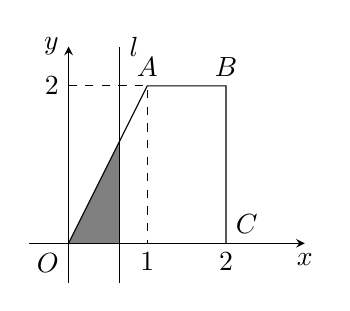
\begin{tikzpicture}[samples=200,>=stealth]
	\fill [gray] (0,0)--(0.65,0)--(0.65,1.3)--cycle;
	\draw [->] (-0.5,0)--(0,0) node [below left] {$O$} --(3,0) node [below] {$x$};
	\draw [->] (0,-0.5)--(0,2.5) node [left] {$y$};
	\draw (0,0)--(1,2) node [above] {$A$}--(2,2) node [above] {$B$}--(2,0) node [above right] {$C$};
	\draw (0.65,-0.5)--(0.65,2.5) node [right] {$l$};
	\draw [dashed] (0,2) node [left] {$2$} --(1,2)--(1,0) node [below] {$1$};
	\draw (2,0) node [below] {$2$};
	
	\end{tikzpicture}
\end{center}
则函数$S=f(t)$的图像大致为\blank{30}.
\fourch{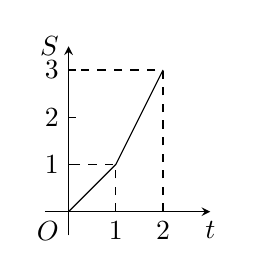
\begin{tikzpicture}[>=stealth]
	\draw [->] (-0.3,0)--(0,0) node [below left] {$O$} --(1.8,0) node [below] {$t$};
	\draw [->] (0,-0.3)--(0,2.1) node [left] {$S$};
	\draw (0.6,0) node [below] {$1$}--(0.6,0.1);
	\draw (1.2,0) node [below] {$2$}--(1.2,0.1);
	\draw (0,0.6) node [left] {$1$}--(0.1,0.6);
	\draw (0,1.2) node [left] {$2$}--(0.1,1.2);
	\draw (0,1.8) node [left] {$3$}--(0.1,1.8);
	\draw (0,0)--(0.6,0.6)--(1.2,1.8);
	\draw [dashed] (0.6,0)--(0.6,0.6)--(0,0.6);
	\draw [dashed] (1.2,0)--(1.2,1.8)--(0,1.8);
	\end{tikzpicture}}{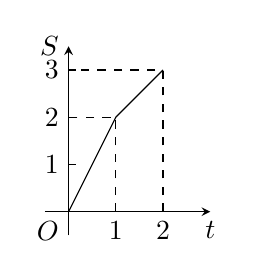
\begin{tikzpicture}[>=stealth]
	\draw [->] (-0.3,0)--(0,0) node [below left] {$O$} --(1.8,0) node [below] {$t$};
	\draw [->] (0,-0.3)--(0,2.1) node [left] {$S$};
	\draw (0.6,0) node [below] {$1$}--(0.6,0.1);
	\draw (1.2,0) node [below] {$2$}--(1.2,0.1);
	\draw (0,0.6) node [left] {$1$}--(0.1,0.6);
	\draw (0,1.2) node [left] {$2$}--(0.1,1.2);
	\draw (0,1.8) node [left] {$3$}--(0.1,1.8);
	\draw (0,0)--(0.6,1.2)--(1.2,1.8);
	\draw [dashed] (0.6,0)--(0.6,1.2)--(0,1.2);
	\draw [dashed] (1.2,0)--(1.2,1.8)--(0,1.8);
	\end{tikzpicture}}{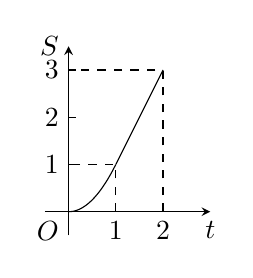
\begin{tikzpicture}[>=stealth,samples=200]
	\draw [->] (-0.3,0)--(0,0) node [below left] {$O$} --(1.8,0) node [below] {$t$};
	\draw [->] (0,-0.3)--(0,2.1) node [left] {$S$};
	\draw (0.6,0) node [below] {$1$}--(0.6,0.1);
	\draw (1.2,0) node [below] {$2$}--(1.2,0.1);
	\draw (0,0.6) node [left] {$1$}--(0.1,0.6);
	\draw (0,1.2) node [left] {$2$}--(0.1,1.2);
	\draw (0,1.8) node [left] {$3$}--(0.1,1.8);
	\draw [domain=0:1] plot ({\x*0.6},{\x*\x*0.6});
	\draw (0.6,0.6)--(1.2,1.8);
	\draw [dashed] (0.6,0)--(0.6,0.6)--(0,0.6);
	\draw [dashed] (1.2,0)--(1.2,1.8)--(0,1.8);
	\end{tikzpicture}}{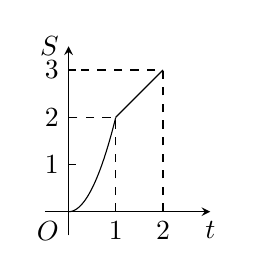
\begin{tikzpicture}[>=stealth,samples=200]
	\draw [->] (-0.3,0)--(0,0) node [below left] {$O$} --(1.8,0) node [below] {$t$};
	\draw [->] (0,-0.3)--(0,2.1) node [left] {$S$};
	\draw (0.6,0) node [below] {$1$}--(0.6,0.1);
	\draw (1.2,0) node [below] {$2$}--(1.2,0.1);
	\draw (0,0.6) node [left] {$1$}--(0.1,0.6);
	\draw (0,1.2) node [left] {$2$}--(0.1,1.2);
	\draw (0,1.8) node [left] {$3$}--(0.1,1.8);
	\draw [domain=0:1] plot ({\x*0.6},{2*\x*\x*0.6});
	\draw (0.6,1.2)--(1.2,1.8);
	\draw [dashed] (0.6,0)--(0.6,1.2)--(0,1.2);
	\draw [dashed] (1.2,0)--(1.2,1.8)--(0,1.8);
	\end{tikzpicture}}


关联目标:

暂未关联目标



标签: 第二单元

答案: 暂无答案

解答或提示: 暂无解答与提示

使用记录:

暂无使用记录


出处: 2016年双基百分百
\item { (003865)}集合$\{y|y=2^{-x}\}\cap\{y|y=\lg x, \ 0<x<100\}=$\blank{50}.


关联目标:

暂未关联目标



标签: 第二单元

答案: 暂无答案

解答或提示: 暂无解答与提示

使用记录:

暂无使用记录


出处: 2016年双基百分百
\item { (003869)}函数$f(x)=a^x+b \ (a>1, \ b<-1)$, 则$y=f^{-1}(x)$的图像一定不经过第\blank{50}象限.


关联目标:

暂未关联目标



标签: 第二单元

答案: 暂无答案

解答或提示: 暂无解答与提示

使用记录:

暂无使用记录


出处: 2016年双基百分百
\item { (003881)}要使$y=x^2+4x \ (x\ge a)$有反函数, 则$a$的最小值为\blank{50}.


关联目标:

暂未关联目标



标签: 第二单元

答案: 暂无答案

解答或提示: 暂无解答与提示

使用记录:

暂无使用记录


出处: 2016年双基百分百
\item { (003884)}已知函数$y=f(x)$的定义域为$\{x|-3\le x\le 8, \ x\ne 5\}$, 值域为$\{y|-1\le y\le 2, \ y\ne 0\}$. 下列关于函数$y=f(x)$的说法: \textcircled{1} 当$x=-3$时, $y=-1$; \textcircled{2} 将$y=f(x)$的图像补上$(5,0)$, 得到的图像必定是一条连续的曲线; \textcircled{3} $y=f(x)$是$[-3,5)$上的单调函数; \textcircled{4} $y=f(x)$的图像与坐标轴只有一个交点. 其中正确的命题是\blank{50}.


关联目标:

暂未关联目标



标签: 第二单元

答案: 暂无答案

解答或提示: 暂无解答与提示

使用记录:

暂无使用记录


出处: 2016年双基百分百
\item { (003889)}已知函数$f(x)=\begin{cases}ax^2-2x-1, & x\ge 0,\\ x^2+bx+c, & x<0\end{cases}$是偶函数, 直线$y=t$与函数$y=f(x)$的图像自左向右依次交于四个不同点$A,B,C,D$. 若$AB=BC$, 则实数$t$的值为\blank{50}.


关联目标:

暂未关联目标



标签: 第二单元

答案: 暂无答案

解答或提示: 暂无解答与提示

使用记录:

暂无使用记录


出处: 2016年双基百分百
\item { (003892)}已知函数$f(x)$是定义在$(-\infty,0)\cup (0,+\infty)$上的偶函数, 当$x>0$时, $f(x)=\begin{cases}
2^{|x-1|}-1, & 0<x\le 2,\\\dfrac 12f(x-2), & x>2,
\end{cases}$ 则函数$g(x)=4f(x)-1$的零点的个数为\blank{30}.
\fourch{$4$}{$6$}{$8$}{$10$}


关联目标:

暂未关联目标



标签: 第二单元

答案: 暂无答案

解答或提示: 暂无解答与提示

使用记录:

暂无使用记录


出处: 2016年双基百分百
\item { (003894)}对于函数$f(x)=ax^2+(b+1)x+b-2 \ (a\ne 0)$, 若存在实数$x_0$, 使$f(x_0)=x_0$成立, 则称$x_0$为$f(x)$的不动点.\\
(1) 若对于任何实数$b$, 函数$f(x)$恒有两个相异的不动点, 求实数$a$的取值范围;\\
(2) 在(1)的条件下, 若函数$y=f(x)$的图像上$A,B$两点的横坐标是函数$f(x)$的不动点, 且直线$y=kx+\dfrac{1}{2a^2+1}$是线段$AB$的垂直平分线, 求实数$b$的取值范围.


关联目标:

暂未关联目标



标签: 第二单元

答案: 暂无答案

解答或提示: 暂无解答与提示

使用记录:

暂无使用记录


出处: 2016年双基百分百
\item { (003896)}函数$y=x^2+4x \ (x<-3)$的反函数为\blank{50}.


关联目标:

暂未关联目标



标签: 第二单元

答案: 暂无答案

解答或提示: 暂无解答与提示

使用记录:

暂无使用记录


出处: 2016年双基百分百
\item { (003907)}设$f(x)$是定义在$\mathbf{R}$上的函数, 且对任意实数$x$, 恒有$f(x+2)=-3f(x)$. 当$x\in [0,2]$时, $f(x)=2x-x^2$, 则$f(0)+f(-1)+f(-2)+\cdots+f(-2014)=$\blank{30}.
\fourch{$-\dfrac 34(1-3^{1007})$}{$-\dfrac 34(1+3^{1007})$}{$-\dfrac 14\left(1-\dfrac{1}{3^{1007}}\right)$}{$-\dfrac 14\left(1+\dfrac{1}{3^{1007}}\right)$}


关联目标:

暂未关联目标



标签: 第二单元

答案: 暂无答案

解答或提示: 暂无解答与提示

使用记录:

暂无使用记录


出处: 2016年双基百分百
\item { (003911)}已知函数$f(x)=\begin{cases}
2^x-1, & x\ge 0,\\ -x^2-2x, & x<0,
\end{cases}$ 若$f(a)=1$, 则实数$a$的值是\blank{50}.


关联目标:

暂未关联目标



标签: 第二单元

答案: 暂无答案

解答或提示: 暂无解答与提示

使用记录:

暂无使用记录


出处: 2016年双基百分百
\item { (003921)}已知函数$f(x)=\dfrac{x}{1+|x|} \ (x\in \mathbf{R})$时, 则下列结论{\bf 不正确}的是\blank{30}.
\onech{任意$x\in \mathbf{R}$, 等式$f(-x)+f(x)=0$恒成立}{存在$m\in (0,1)$, 使得方程$|f(x)|=m$有两个不等实数根}{对任意$x_1,x_2\in \mathbf{R}$, 若$x_1\ne x_2$, 则一定有$f(x_1)\ne f(x_2)$}{存在$k\in (1,+\infty)$, 使得函数$g(x)=f(x)-kx$在$\mathbf{R}$上三个零点}


关联目标:

暂未关联目标



标签: 第二单元

答案: 暂无答案

解答或提示: 暂无解答与提示

使用记录:

暂无使用记录


出处: 2016年双基百分百
\item { (003936)}函数$y=\ln(\cos x) \ \left(-\dfrac{\pi}{2}<x<\dfrac{\pi}{2}\right)$的大致图像是\blank{30}.
\fourch{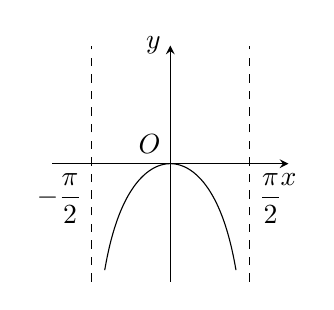
\begin{tikzpicture}[samples=200,>=stealth]
	\draw [->](-1.5,0)--(0,0) node [above left] {$O$}--(1.5,0) node [below] {$x$};
	\draw [->](0,-1.5)--(0,1.5) node [left] {$y$};
	\draw [dashed] (-1,-1.5)--(-1,1.5) (1,-1.5)--(1,1.5);
	\draw (-1,0) node [below left] {$-\dfrac{\pi}{2}$};
	\draw (1,0) node  [below right] {$\dfrac{\pi}{2}$};
	\draw [domain=-75:75] plot ({\x/90},{ln(cos(\x))});
	\end{tikzpicture}}{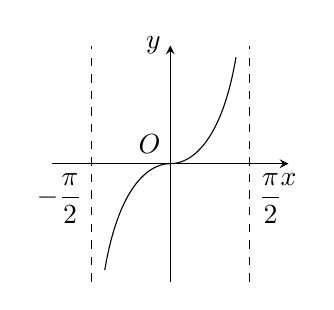
\begin{tikzpicture}[samples=200,>=stealth]
	\draw [->](-1.5,0)--(0,0) node [above left] {$O$}--(1.5,0) node [below] {$x$};
	\draw [->](0,-1.5)--(0,1.5) node [left] {$y$};
	\draw [dashed] (-1,-1.5)--(-1,1.5) (1,-1.5)--(1,1.5);
	\draw (-1,0) node [below left] {$-\dfrac{\pi}{2}$};
	\draw (1,0) node  [below right] {$\dfrac{\pi}{2}$};
	\draw [domain=-75:0] plot ({\x/90},{ln(cos(\x))});
	\draw [domain=0:75] plot ({\x/90},{-ln(cos(\x))});
	\end{tikzpicture}}{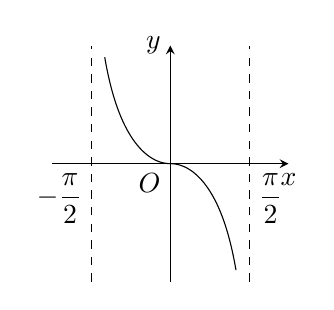
\begin{tikzpicture}[samples=200,>=stealth]
	\draw [->](-1.5,0)--(0,0) node [below left] {$O$}--(1.5,0) node [below] {$x$};
	\draw [->](0,-1.5)--(0,1.5) node [left] {$y$};
	\draw [dashed] (-1,-1.5)--(-1,1.5) (1,-1.5)--(1,1.5);
	\draw (-1,0) node [below left] {$-\dfrac{\pi}{2}$};
	\draw (1,0) node  [below right] {$\dfrac{\pi}{2}$};
	\draw [domain=-75:0] plot ({\x/90},{-ln(cos(\x))});
	\draw [domain=0:75] plot ({\x/90},{ln(cos(\x))});
	\end{tikzpicture}}{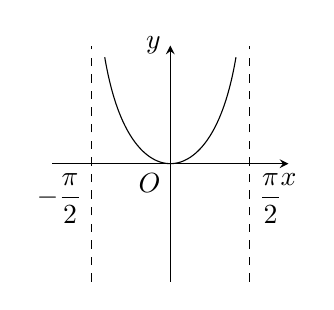
\begin{tikzpicture}[samples=200,>=stealth]
	\draw [->](-1.5,0)--(0,0) node [below left] {$O$}--(1.5,0) node [below] {$x$};
	\draw [->](0,-1.5)--(0,1.5) node [left] {$y$};
	\draw [dashed] (-1,-1.5)--(-1,1.5) (1,-1.5)--(1,1.5);
	\draw (-1,0) node [below left] {$-\dfrac{\pi}{2}$};
	\draw (1,0) node  [below right] {$\dfrac{\pi}{2}$};
	\draw [domain=-75:75] plot ({\x/90},{-ln(cos(\x))});
	\end{tikzpicture}}


关联目标:

暂未关联目标



标签: 第二单元

答案: 暂无答案

解答或提示: 暂无解答与提示

使用记录:

暂无使用记录


出处: 2016年双基百分百
\item { (003953)}已知集合$M$是满足下列性质的函数$f(x)$的全体, 存在非零常数$T$, 对任意$x\in \mathbf{R}$, 有$f(x+T)=Tf(x)$成立.\\
(1) 函数$f(x)=x$是否属于集合$M$? 说明理由;\\
(2) 设$f(x)\in M$, 且$T=2$, 已知当$1<x<2$时, $f(x)=x+\ln x$, 求当$-3<x<-2$时, $f(x)$的解析式.


关联目标:

暂未关联目标



标签: 第二单元

答案: 暂无答案

解答或提示: 暂无解答与提示

使用记录:

暂无使用记录


出处: 2016年双基百分百
\item { (003966)}(理科)已知函数$f(x)$是定义在$\mathbf{R}$上的单调递减函数且为奇函数, 数列$\{a_n\}$是等差数列, $a_{1007}>0$, 则$f(a_1)+f(a_2)+f(a_3)+\cdots+f(a_{2012})+f(a_{2013})$的值\blank{30}.
\fourch{恒为正数}{恒为负数}{恒为$0$}{可正可负}


关联目标:

暂未关联目标



标签: 第二单元

答案: 暂无答案

解答或提示: 暂无解答与提示

使用记录:

暂无使用记录


出处: 2016年双基百分百
\item { (003981)}(理科)在方程为$\begin{cases}
x=\sin 2\theta,\\ y=\sin\theta+\cos\theta
\end{cases}$的曲线上的点是\blank{30}.
\fourch{$(2,\sqrt{3})$}{$(1,\sqrt{3})$}{$\left(-\dfrac 34,\dfrac 12\right)$}{$\left(\dfrac 12,-\sqrt{2}\right)$}\\
(文科)若函数$y=f(x)$存在反函数, 则方程$f(x)=c$($c$为常数)\blank{30}.
\fourch{有且只有一个实根}{至少有一个实根}{至多有一个实根}{没有实数根}


关联目标:

暂未关联目标



标签: 第二单元|第七单元

答案: 暂无答案

解答或提示: 暂无解答与提示

使用记录:

暂无使用记录


出处: 2016年双基百分百
\item { (004067)}已知定义在$\mathbf{R}$上的函数$f(x)$满足: \textcircled{1} $f(x)+f(2-x)=0$; \textcircled{2} $f(x)-f(-2-x)=0$; \textcircled{3} 在$[-1,1]$上表达式为$f(x)=\begin{cases} \sqrt{1-x^2}, & x\in [-1,0], \\ 1-x, & x\in (0,1], \end{cases}$ 则函数$f(x)$与$g(x)=\begin{cases} {2^x}, & x\le 0 \\ \log_\frac 12x, & x>0 \end{cases}$的图像在区间$[-3,3]$上的交点的个数为\blank{50}.


关联目标:

暂未关联目标



标签: 第二单元

答案: $6$

解答或提示: 暂无解答与提示

使用记录:

20220301	2022届高三1班	\fcolorbox[rgb]{0,0,0}{1.000,0.838,0}{0.581}


出处: 2022届高三下学期测验卷01第9题
\item { (004070)}已知$f(x)=2x^2+2x+b$是定义在$[-1,0]$上的函数, 若$f[f(x)]\le 0$在定义域上恒成立, 而且存在实数$x_0$满足: $f[f(x_0)]=x_0$且$f(x_0)\ne x_0$, 则实数$b$的取值范围是\blank{50}.


关联目标:

暂未关联目标



标签: 第二单元

答案: $[-\dfrac12,-\dfrac 38)$

解答或提示: 暂无解答与提示

使用记录:

20220301	2022届高三1班	\fcolorbox[rgb]{0,0,0}{0.000,1.000,0}{0.000}


出处: 2022届高三下学期测验卷01第12题
\item { (004074)}如图, 在直角坐标平面内有一个边长为$a$, 中心在原点$O$的
正六边形$ABCDEF$, $AB\parallel Ox$. 直线$l:y=kx+t$ ($k$是常数)与正六边形交于$M$、$N$两点, 记$\triangle OMN$的面积为$S$, 则函数$S=f(t)$的奇偶性为\bracket{20}.
\begin{center}
    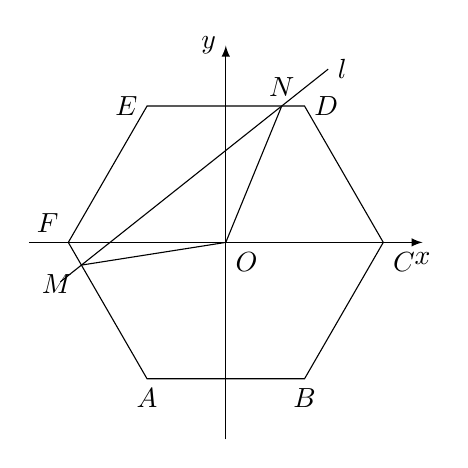
\begin{tikzpicture}[>=latex]
        \draw [->] (-2.5,0) -- (2.5,0) node [below] {$x$};
        \draw [->] (0,-2.5) -- (0,2.5) node [left] {$y$};
        \draw (0,0) node [below right] {$O$};
        \draw [name path = hexagon] (-1,{-sqrt(3)}) node [below] {$A$} -- (1,{-sqrt(3)}) node [below] {$B$} -- (2,0) node [below right] {$C$} -- (1,{sqrt(3)}) node [right] {$D$} -- (-1,{sqrt(3)}) node [left] {$E$} -- (-2,0) node [above left] {$F$} -- cycle;
        \draw [name path = linel] (-2.1,-0.5) -- (1.3,2.2)node [right] {$l$};
        \path [name intersections = {of = hexagon and linel, by = {N,M}}];
        \draw (N) node [above] {$N$} -- (0,0) -- (M) node [below left] {$M$};
    \end{tikzpicture}
\end{center}
\twoch{偶函数}{奇函数}{不是奇函数, 也不是偶函数}{奇偶性与$k$有关}


关联目标:

暂未关联目标



标签: 第二单元|第七单元

答案: A

解答或提示: 暂无解答与提示

使用记录:

20220301	2022届高三1班	\fcolorbox[rgb]{0,0,0}{1.000,0.094,0}{0.953}


出处: 2022届高三下学期测验卷01第16题
\item { (004079)}已知函数$f(x)=\log_2x$.\\
(1) 若$f(x)$的反函数是$f^{-1}(x)$, 解方程: $f^{-1}(2x+1)=3f^{-1}(x)-1$;\\
(2) 当$x\in (3m, 3m+3]$($m\in \mathbf{N}$)时, 定义$g(x)=f(x-3m)$. 设$a_n=n\cdot g(n)$, 数列$\{a_n\}$ 的前$n$项和为$S_n$, 求$a_1$、$a_2$、$a_3$、$a_4$和$S_{3n}$;\\
(3) 对于任意$a$、$b$、$c\in [M,+\infty)$, 且$a\ge b\ge c$. 当$a$、$b$、$c$能作为一个三角形的三边长时, $f(a)$、$f(b)$、$f(c)$也总能作为某个三角形的三边长, 试探究$M$的最小值.


关联目标:

暂未关联目标



标签: 第二单元

答案: (1) 解为$-1$和$0$; (2) $a_1=0$, $a_2=2$, $a_3=3\log_2 3$, $a_4=0$, $S_{3n}=\dfrac 12 n(3n+1+(3n+3)\log_2 3)$; (3) $M$的最小值为$2$.

解答或提示: 暂无解答与提示

使用记录:

20220301	2022届高三1班	\fcolorbox[rgb]{0,0,0}{1.000,0.046,0}{0.977}	\fcolorbox[rgb]{0,0,0}{1.000,0.504,0}{0.748}	\fcolorbox[rgb]{0,0,0}{0.284,1.000,0}{0.142}


出处: 2022届高三下学期测验卷01第21题
\item { (004086)}已知函数$f(x)=\begin{cases} 2^x, & x\le 0 \\  \log_2x, & 0<x\le 1 \end{cases}$的反函数是$f^{-1}(x)$, 则$f^{-1}(\dfrac 12)=$\blank{50}.


关联目标:

暂未关联目标



标签: 第二单元

答案: 暂无答案

解答或提示: 暂无解答与提示

使用记录:

20220308	2022届高三1班	\fcolorbox[rgb]{0,0,0}{1.000,0.000,0}{1.000}


出处: 2022届高三下学期测验卷02第7题
\item { (004089)}$[x]$是不超过$x$的最大整数, 则方程$(2^x)^2-\dfrac 74\cdot [2^x]-\dfrac 14=0$满足$x<1$的所有实数解是\blank{50}.


关联目标:

暂未关联目标



标签: 第二单元

答案: 暂无答案

解答或提示: 暂无解答与提示

使用记录:

20220308	2022届高三1班	\fcolorbox[rgb]{0,0,0}{1.000,0.186,0}{0.907}


出处: 2022届高三下学期测验卷02第10题
\item { (004090)}在直角$\triangle ABC$中, $\angle A=\dfrac{\pi}2$, $AB=1$, $AC=2$, $M$是$\triangle ABC$内一点, 且$AM=\dfrac 12$, 若$\overrightarrow{AM}=\lambda \overrightarrow{AB}+\mu \overrightarrow{AC}$, 则$\lambda +2\mu$的最大值为\blank{50}.


关联目标:

暂未关联目标



标签: 第二单元|第五单元

答案: 暂无答案

解答或提示: 暂无解答与提示

使用记录:

20220308	2022届高三1班	\fcolorbox[rgb]{0,0,0}{1.000,0.418,0}{0.791}


出处: 2022届高三下学期测验卷02第11题
\item { (004091)}已知函数$f(x)=\cos x$, 若对任意实数$x_1$、$x_2$, 方程$|f(x)-f(x_1)|+|f(x)-f(x_2)|=m$($m\in \mathbf{R}$)有解, 方程$|f(x)-f(x_1)|-|f(x)-f(x_2)|=n$($n\in \mathbf{R}$)也有解, 则$m+n$的值的集合为\blank{50}.


关联目标:

暂未关联目标



标签: 第二单元

答案: 暂无答案

解答或提示: 暂无解答与提示

使用记录:

20220308	2022届高三1班	\fcolorbox[rgb]{0,0,0}{0.652,1.000,0}{0.326}


出处: 2022届高三下学期测验卷02第12题
\item { (004094)}已知$f(x)$是定义在$\mathbf{R}$上的奇函数, 对任意两个不相等的正数$x_1$, $x_2$都有$\dfrac{x_2f(x_1)-x_1f(x_2)}{x_1-x_2}<0$, 则函数$g(x)=\begin{cases} \dfrac{f(x)}x, &x\ne 0, \\ 0, & x=0 \end{cases}$\bracket{20}.
\twoch{是偶函数, 且在$(0,+\infty)$上单调递减}{是偶函数, 且在$(0,+\infty)$上单调递增}{是奇函数, 且单调递减}{是奇函数, 且单调递增}


关联目标:

暂未关联目标



标签: 第二单元

答案: 暂无答案

解答或提示: 暂无解答与提示

使用记录:

20220308	2022届高三1班	\fcolorbox[rgb]{0,0,0}{1.000,0.140,0}{0.930}


出处: 2022届高三下学期测验卷02第15题
\item { (004097)}已知函数$f(x)=1-\dfrac 6{a^{x+1}+a}$($a>0$, $a\ne 1$)是定义在$\mathbf{R}$上的奇函数.\\
(1) 求实数$a$的值及函数$f(x)$的值域;\\
(2) 若不等式 $t\cdot f(x)\ge 3^x-3$在$x\in [1,2]$上恒成立, 求实数$t$的取值范围.


关联目标:

暂未关联目标



标签: 第二单元

答案: 暂无答案

解答或提示: 暂无解答与提示

使用记录:

20220308	2022届高三1班	\fcolorbox[rgb]{0,0,0}{1.000,0.032,0}{0.984}	\fcolorbox[rgb]{0,0,0}{1.000,0.104,0}{0.948}


出处: 2022届高三下学期测验卷02第18题
\item { (004102)}已知函数$f(x)=\sqrt{2x-1}$的反函数为$f^{-1}(x)$ , 则$f^{-1}(7)=$\blank{50}.


关联目标:

暂未关联目标



标签: 第二单元

答案: 暂无答案

解答或提示: 暂无解答与提示

使用记录:

暂无使用记录


出处: 2022届高三下学期测验卷03第2题
\item { (004106)}方程$\log_5(4^x-11)-1=\log_5(2^x-3)$的解为$x=$\blank{50}.


关联目标:

暂未关联目标



标签: 第二单元

答案: 暂无答案

解答或提示: 暂无解答与提示

使用记录:

暂无使用记录


出处: 2022届高三下学期测验卷03第6题
\item { (004108)}已知函数$f(x)=g(x)+|2x-1|$为奇函数, 若$g(-2)=7$, 则$g(2)=$\blank{50}.


关联目标:

暂未关联目标



标签: 第二单元

答案: 暂无答案

解答或提示: 暂无解答与提示

使用记录:

暂无使用记录


出处: 2022届高三下学期测验卷03第8题
\item { (004116)}已知集合$M=\{(x,y)|y=f(x)\}$, 若对于任意$(x_1,y_1)\in M$, 存在$(x_2,y_2)\in M$, 使得$x_1x_2+y_1y_2=0$成立, 则称集合$M$是``$\Omega$集合''. 给出下列$4$个集合:
\textcircled{1} $M=\{(x,y) |y=\dfrac 1x \}$; \textcircled{2} $M=\{(x,y)|y=\mathrm{e}^x-2\}$; \textcircled{3} $M=\{(x,y)|y=\cos x\}$; \textcircled{4} $M=\{(x,y)|y=\ln x\}$.
其中所有``$\Omega$集合''的序号是\bracket{20}.
\fourch{\textcircled{2}\textcircled{3}}{\textcircled{3}\textcircled{4}}{\textcircled{1}\textcircled{2}\textcircled{4}}{\textcircled{1}\textcircled{3}\textcircled{4}}


关联目标:

暂未关联目标



标签: 第二单元

答案: 暂无答案

解答或提示: 暂无解答与提示

使用记录:

20220322	2022届高三1班	\fcolorbox[rgb]{0,0,0}{1.000,0.140,0}{0.930}


出处: 2022届高三下学期测验卷03第16题
\item { (004118)}已知$f(x)=ax+\dfrac{x^2}{x^2+1}$, $a$为实常数.\\
(1) 当$a=1$时, 求不等式$f(x)+f(\dfrac 1x)<x$的解集;\\
(2) 若函数$f(x)$在$(0,+\infty)$中有零点, 求$a$的取值范围.


关联目标:

暂未关联目标



标签: 第二单元

答案: 暂无答案

解答或提示: 暂无解答与提示

使用记录:

暂无使用记录


出处: 2022届高三下学期测验卷03第18题
\item { (004130)}已知常数$b,c\in \mathbf{R}$. 若函数$f(x)=(x^2+x-2)(x^2+bx+c)$为偶函数, 则$b+c=$\blank{50}.


关联目标:

暂未关联目标



标签: 第二单元

答案: 暂无答案

解答或提示: 暂无解答与提示

使用记录:

20220331	2022届高三1班	\fcolorbox[rgb]{0,0,0}{1.000,0.094,0}{0.953}


出处: 2022届高三下学期测验卷04第9题
\item { (004139)}已知常数$a\in \mathbf{R}^+$, 函数$f(x)=3^x+a^2\cdot 3^{-x}$.\\
(1) 若$a=\sqrt{3}$, 解关于$x$的不等式$f(x)<4$;\\
(2) 若$f(x)$在$[3,+\infty)$上为增函数, 求$a$的取值范围.


关联目标:

暂未关联目标



标签: 第二单元

答案: 暂无答案

解答或提示: 暂无解答与提示

使用记录:

20220331	2022届高三1班	\fcolorbox[rgb]{0,0,0}{1.000,0.086,0}{0.957}	\fcolorbox[rgb]{0,0,0}{1.000,0.290,0}{0.855}


出处: 2022届高三下学期测验卷04第18题
\item { (004143)}方程$\log_3(2x+1)=2$的解是\blank{50}.


关联目标:

暂未关联目标



标签: 第二单元

答案: 暂无答案

解答或提示: 暂无解答与提示

使用记录:

20220407	2022届高三1班	\fcolorbox[rgb]{0,0,0}{1.000,0.046,0}{0.977}


出处: 2022届高三下学期测验卷05第1题
\item { (004149)}若函数$f(x)=2^x(x+a)-1$在区间$[0,1]$上有零点, 则实数$a$的取值范围是\blank{50}.


关联目标:

暂未关联目标



标签: 第二单元

答案: 暂无答案

解答或提示: 暂无解答与提示

使用记录:

20220407	2022届高三1班	\fcolorbox[rgb]{0,0,0}{1.000,0.046,0}{0.977}


出处: 2022届高三下学期测验卷05第7题
\item { (004151)}设不等式组$\begin{cases} x+y-6\ge 0, \\ x-y+2\ge 0, \\ x-3y+6\le 0 \end{cases}$表示的可行域为$\Omega$, 若指数函数$y=a^x$的图像与$\Omega$有公共点, 则$a$的取值范围是\blank{50}.


关联目标:

暂未关联目标



标签: 第二单元

答案: 暂无答案

解答或提示: 暂无解答与提示

使用记录:

20220407	2022届高三1班	\fcolorbox[rgb]{0,0,0}{1.000,0.418,0}{0.791}


出处: 2022届高三下学期测验卷05第9题
\item { (004153)}已知$f(x)=1+ax-\sqrt{1+ax^2}$, 若对任意$x\in [0,\sqrt 2]$, $f(x)\le 0$恒成立, 则实数$a$的取值范围为\blank{50}.


关联目标:

暂未关联目标



标签: 第二单元

答案: 暂无答案

解答或提示: 暂无解答与提示

使用记录:

20220407	2022届高三1班	\fcolorbox[rgb]{0,0,0}{1.000,0.652,0}{0.674}


出处: 2022届高三下学期测验卷05第11题
\item { (004155)}函数$y=x^2(x\le 0)$的反函数为\bracket{20}.
\fourch{$y=\sqrt{x}, \ x\ge 0$}{$y=-\sqrt{x}, \ x\ge 0$}{$y=\sqrt{x}, \ x\le 0$}{$y=-\sqrt{x}, \ x\le 0$}


关联目标:

暂未关联目标



标签: 第二单元

答案: 暂无答案

解答或提示: 暂无解答与提示

使用记录:

20220407	2022届高三1班	\fcolorbox[rgb]{0,0,0}{1.000,0.000,0}{1.000}


出处: 2022届高三下学期测验卷05第13题
\item { (004157)}已知函数$f(x)=x+\dfrac ax$($a>0$), $0<x_1<x_2$, 且$f(x_1)=f(x_2)$, 给出以下结论:\\
\textcircled{1} $\dfrac{x_1+x_2}2>\sqrt a$恒成立; \textcircled{2} $f(2\sqrt a-x_1)<f(x_2)$恒成立. 则\bracket{20}.
\fourch{\textcircled{1}正确, \textcircled{2}正确}{\textcircled{1}正确, \textcircled{2}错误}{\textcircled{1}错误, \textcircled{2}正确}{\textcircled{1}错误, \textcircled{2}错误}


关联目标:

暂未关联目标



标签: 第二单元

答案: 暂无答案

解答或提示: 暂无解答与提示

使用记录:

20220407	2022届高三1班	\fcolorbox[rgb]{0,0,0}{1.000,0.094,0}{0.953}


出处: 2022届高三下学期测验卷05第15题
\item { (004161)}某学校对面有一块空地要围建成一个面积为$360\text{m}^2$的矩形场地, 要求矩形场地的一面利用旧墙(旧墙需要整修), 其它三面围墙要新建, 在旧墙对面的新墙上要留一个宽度为$2\text{m}$的进出口, 如图所示. 已知旧墙的整修费用为$45\text{元/m}$, 新建墙的造价为$180\text{元/m}$, 建$2\text{m}$宽的进出口需$2360$元的单独费用, 设利用的旧墙的长度为$x$(单位: $\text{m}$), 设修建此矩形场地围墙的总费用(含建进出口的费用)为$y$(单位: 元).\\
\begin{center}
    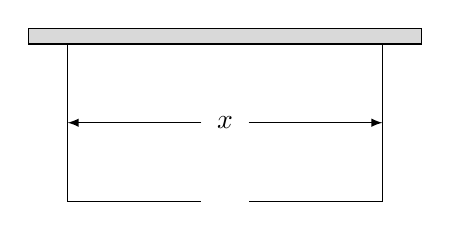
\begin{tikzpicture}[>=latex]
        \filldraw [gray!30] (0,0) rectangle (5,0.2);
        \draw (0,0) rectangle (5,0.2);
        \draw (0.5,0) -- (0.5,-2) -- (2.2,-2) (4.5,0) -- (4.5,-2) -- (2.8,-2);
        \draw (2.5,-1) node {$x$};
        \draw [->] (2.2,-1) -- (0.5,-1);
        \draw [->] (2.8,-1) -- (4.5,-1); 
    \end{tikzpicture}
\end{center}
(1) 将$y$表示为$x$的函数;\\
(2) 试确定$x$, 使修建此矩形场地围墙的总费用(含建进出口的费用)最少, 并求出最少总费用.


关联目标:

暂未关联目标



标签: 第二单元

答案: 暂无答案

解答或提示: 暂无解答与提示

使用记录:

20220407	2022届高三1班	\fcolorbox[rgb]{0,0,0}{1.000,0.180,0}{0.910}	\fcolorbox[rgb]{0,0,0}{1.000,0.148,0}{0.926}


出处: 2022届高三下学期测验卷05第19题
\item { (004165)}已知函数$f(x)=\log_3(\dfrac 4{x+2})$ , 则方程$f^{-1}(x)=4$的解$x=$\blank{50}.


关联目标:

暂未关联目标



标签: 第二单元

答案: 暂无答案

解答或提示: 暂无解答与提示

使用记录:

20220421	2022届高三1班	\fcolorbox[rgb]{0,0,0}{1.000,0.046,0}{0.977}


出处: 2022届高三下学期测验卷06第2题
\item { (004175)}已知实数$a$、$b$使得不等式$|ax^2+bx+a|\le x$对任意$x\in [1,2]$都成立, 在平面直角坐标系$xOy$中, 点$(a,b)$形成的区域记为$\Omega$, 若圆$x^2+y^2=r^2$上的任一点都在$\Omega$中, 则$r$的最大值为\blank{50}


关联目标:

暂未关联目标



标签: 第二单元|第七单元

答案: 暂无答案

解答或提示: 暂无解答与提示

使用记录:

20220421	2022届高三1班	\fcolorbox[rgb]{0,0,0}{1.000,0.558,0}{0.721}


出处: 2022届高三下学期测验卷06第12题
\item { (004179)}已知定义在实数集$\mathbf{R}$上的函数$f(x)$满足$f(x+1)=\dfrac 12+\sqrt{f(x)-f^2(x)}$, 则$f(0)+f(2021)$的最小值与最大值的和为\bracket{20}.
\fourch{$2$}{$3$}{$\dfrac 32+\dfrac{\sqrt 2}2$}{$\dfrac 52+\dfrac{\sqrt 2}2$}


关联目标:

暂未关联目标



标签: 第二单元

答案: 暂无答案

解答或提示: 暂无解答与提示

使用记录:

20220421	2022届高三1班	\fcolorbox[rgb]{0,0,0}{0.326,1.000,0}{0.163}


出处: 2022届高三下学期测验卷06第16题
\item { (004184)}设$m$为给定的实常数, 若函数$y=f(x)$在其定义域内存在实数$x_0$, 使得$f(x_0+m)=f(x_0)+f(m)$成立, 则称函数$f(x)$为``$G(m)$函数''.\\
(1) 若函数$f(x)=2^x$为``$G(2)$函数'', 求实数$x_0$的值;\\
(2) 若函数$f(x)=\lg \dfrac a{x^2+1}$为``$G(1)$函数'', 求实数$a$的取值范围;\\
(3) 已知$f(x)=x+b$($b\in \mathbf{R}$)为``$G(0)$函数'', 设$g(x)=x|x-4|$. 若对任意的$x_1,x_2\in[0,t]$, 当$x_1\ne x_2$时, 都有$\dfrac{g(x_1)-g(x_2)}{f(x_1)-f(x_2)}>2$成立, 求实数$t$的最大值.


关联目标:

暂未关联目标



标签: 第二单元

答案: 暂无答案

解答或提示: 暂无解答与提示

使用记录:

20220421	2022届高三1班	\fcolorbox[rgb]{0,0,0}{1.000,0.012,0}{0.994}	\fcolorbox[rgb]{0,0,0}{1.000,0.520,0}{0.740}	\fcolorbox[rgb]{0,0,0}{1.000,0.734,0}{0.633}


出处: 2022届高三下学期测验卷06第21题
\item { (004191)}某种微生物的日增长率为$r$, 经过$n$天后其数量由$p_0$变化为$p$, 并且满足方程$p=p_0\mathrm{e}^{rn}$.实验检测, 这种微生物经过一周数量由$2.58$个单位增长到$14.86$个单位, 则增长率$r=$\blank{50}(精确到$1\%$).


关联目标:

暂未关联目标



标签: 第二单元

答案: 暂无答案

解答或提示: 暂无解答与提示

使用记录:

20220428	2022届高三1班	\fcolorbox[rgb]{0,0,0}{1.000,0.140,0}{0.930}


出处: 2022届高三下学期测验卷07第7题
\item { (004203)}已知函数$f(x)=ax+\log_2(2^x+1)$, 其中$a\in \mathbf{R}$.\\
(1) 根据$a$的不同取值, 讨论$f(x)$的奇偶性, 并说明理由;\\
(2) 已知$a>0$, 函数$f(x)$的反函数为$f^{-1}(x)$, 若函数$y=f(x)+f^{-1}(x)$在区间$[1,2]$上的最小值为$1+\log_23$, 求函数$f(x)$在区间$[1,2]$上的最大值.


关联目标:

暂未关联目标



标签: 第二单元

答案: 暂无答案

解答或提示: 暂无解答与提示

使用记录:

20220428	2022届高三1班	\fcolorbox[rgb]{0,0,0}{1.000,0.032,0}{0.984}	\fcolorbox[rgb]{0,0,0}{1.000,0.466,0}{0.767}


出处: 2022届高三下学期测验卷07第19题
\item { (004214)}设定义域为$\mathbf{R}$的函数$f(x)$、$g(x)$都有反函数, 且函数$f(x-1)$和$g^{-1}(x-3)$图像关于直线$y=x$对称, 若$g(5)=2015$, 则$f(4)=$\blank{50}.


关联目标:

暂未关联目标



标签: 第二单元

答案: 暂无答案

解答或提示: 暂无解答与提示

使用记录:

20220505	2022届高三1班	\fcolorbox[rgb]{0,0,0}{1.000,0.046,0}{0.977}


出处: 2022届高三下学期测验卷08第9题
\item { (004217)}已知函数$f(x)$满足: \textcircled{1} 对任意$x\in (0,+\infty)$恒有$f(2x)=2f(x)$成立; \textcircled{2} $x\in (1,2]$时, $f(x)=2-x$; 若$f(a)=f(2020)$, 则满足条件的最小的正实数$a$是\blank{50}.


关联目标:

暂未关联目标



标签: 第二单元

答案: 暂无答案

解答或提示: 暂无解答与提示

使用记录:

20220505	2022届高三1班	\fcolorbox[rgb]{0,0,0}{1.000,0.186,0}{0.907}


出处: 2022届高三下学期测验卷08第12题
\item { (004220)}已知函数\textcircled{1} $f(x)=3\ln x$; \textcircled{2} $f(x)=3\mathrm{e}^{\cos x}$; \textcircled{3} $f(x)=3\mathrm{e}^x$; \textcircled{4} $f(x)=3\cos x$; 其中对于$f(x)$定义域内的任意一个自变量$x_1$都存在唯一一个自变量$x_2$, 使$\sqrt{f(x_1)f(x_2)}=3$成立的函数是\bracket{20}.
\fourch{\textcircled{3}}{\textcircled{2}\textcircled{3}}{\textcircled{1}\textcircled{2}\textcircled{4}}{\textcircled{4}}


关联目标:

暂未关联目标



标签: 第二单元|第三单元

答案: 暂无答案

解答或提示: 暂无解答与提示

使用记录:

20220505	2022届高三1班	\fcolorbox[rgb]{0,0,0}{1.000,0.140,0}{0.930}


出处: 2022届高三下学期测验卷08第15题
\item { (004224)}对于两个定义域相同的函数$f(x)$、$g(x)$, 若存在实数$m$、$n$, 使$h(x)=mf(x)+ng(x)$, 则称函数$h(x)$是由``基函数$f(x)$、$g(x)$''生成的.\\
(1) $f(x)=x^2+3x$和$g(x)=3x+4$生成一个偶函数$h(x)$, 求$h(2)$的值;\\
(2) 若$h(x)=2x^2+3x-1$由$f(x)=x^2+ax$, $g(x)=x+b$($a,b\in \mathbf{R}$且$ab\ne 0$)生成, 求$a+2b$的取值范围.


关联目标:

暂未关联目标



标签: 第二单元

答案: 暂无答案

解答或提示: 暂无解答与提示

使用记录:

20220505	2022届高三1班	\fcolorbox[rgb]{0,0,0}{1.000,0.100,0}{0.950}	\fcolorbox[rgb]{0,0,0}{1.000,0.486,0}{0.757}


出处: 2022届高三下学期测验卷08第19题
\item { (004228)}函数$f(x)=\sqrt{1-\dfrac 2x}$的定义域是\blank{50}.


关联目标:

暂未关联目标



标签: 第二单元

答案: 暂无答案

解答或提示: 暂无解答与提示

使用记录:

20220512	2022届高三1班	\fcolorbox[rgb]{0,0,0}{1.000,0.232,0}{0.884}


出处: 2022届高三下学期测验卷09第2题
\item { (004229)}函数$y=2^x$($x\ge 2$)的反函数是\blank{50}.


关联目标:

暂未关联目标



标签: 第二单元

答案: 暂无答案

解答或提示: 暂无解答与提示

使用记录:

20220512	2022届高三1班	\fcolorbox[rgb]{0,0,0}{1.000,0.000,0}{1.000}


出处: 2022届高三下学期测验卷09第3题
\item { (004235)}在$\triangle ABC$中, 角$A$、$B$、$C$所对的边分别为$a$、$b$、$c$, 如果对任意的实数$\lambda$, $|\overrightarrow{BA}-\lambda \overrightarrow{BC}|\ge |\overrightarrow{BC}|$恒成立, 则$\dfrac cb+\dfrac bc$的最大值是\blank{50}.


关联目标:

暂未关联目标



标签: 第二单元|第四单元

答案: 暂无答案

解答或提示: 暂无解答与提示

使用记录:

20220512	2022届高三1班	\fcolorbox[rgb]{0,0,0}{0.466,1.000,0}{0.233}


出处: 2022届高三下学期测验卷09第9题
\item { (004238)}对实数$x\in \mathbf{R}$, 函数$f(x)$满足: $f(x+1)=\sqrt{f(x)-{f^2}(x)}+\dfrac 12$, $a_n=f^2(n)-f(n)$,
数列$\{a_n\}$的前$15$项和为$-\dfrac{31}{16}$, 数列$\{c_n\}$满足$c_n+c_{n+1}=[f(2019)]^n$, 若数列$\{c_n\}$的前$n$项和$S_n$的极限存在, 则$c_1=$\blank{50}.


关联目标:

暂未关联目标



标签: 第二单元|第四单元

答案: 暂无答案

解答或提示: 暂无解答与提示

使用记录:

20220512	2022届高三1班	\fcolorbox[rgb]{0,0,0}{0.418,1.000,0}{0.209}


出处: 2022届高三下学期测验卷09第12题
\item { (004247)}设函数$f(x)$在$[1,+\infty)$上有定义, 实数$a$和$b$满足$1\le a<b$, 若$f(x)$在区间$(a,b]$上不存在最小值, 则称$f(x)$在区间$(a,b]$上具有性质$P$.\\
(1) 当$f(x)=x^2+cx$, 且$f(x)$在区间$(1,2]$上具有性质$P$, 求实数$c$的取值范围;\\
(2) 已知$f(x+1)=f(x)+1$($x\ge 1$), 且当$1\le x<2$时, $f(x)=1-x$, 判别$f(x)$在区间$(1,4]$ 上是否具有性质$P$;\\
(3) 若对于满足$1\le a<b$的任意实数$a$和$b$, $f(x)$在区间$(a,b]$上具有性质$P$, 且对于任意$n\in \mathbf{N}^*$, 当$x\in (n,n+1)$时, 有$|f(n)-f(x)|+|f(x)-f(n+1)|=|f(n)-f(n+1)|$, 证明: 当$x\ge 1$时, $f(2x)>f(x)$.


关联目标:

暂未关联目标



标签: 第二单元

答案: 暂无答案

解答或提示: 暂无解答与提示

使用记录:

20220512	2022届高三1班	\fcolorbox[rgb]{0,0,0}{1.000,0.198,0}{0.901}	\fcolorbox[rgb]{0,0,0}{1.000,0.612,0}{0.694}	\fcolorbox[rgb]{0,0,0}{0.064,1.000,0}{0.032}


出处: 2022届高三下学期测验卷09第21题
\item { (004256)}设$f(x)$是定义在$\mathbf{R}$上的奇函数, 当$x>0$时, $f(x)=a^x+b$($0<a<1$, $b\in \mathbf{R}$), 若$f(x)$存在反函数, 则b的取值范围是\blank{50}.


关联目标:

暂未关联目标



标签: 第二单元

答案: 暂无答案

解答或提示: 暂无解答与提示

使用记录:

20220517	2022届高三1班	\fcolorbox[rgb]{0,0,0}{1.000,0.604,0}{0.698}


出处: 2022届高三下学期测验卷10第9题
\item { (004259)}已知定义在$\mathbf{R}$上的函数$f(x)$满足$f(x+1)=2f(x)+1$, 当$x\in [0,1)$时, $f(x)=x^3$. 设$f(x)$在区间$[n,n+1)$($n\in \mathbf{N}^*$)上的最小值为$a_n$, 若存在$n\in \mathbf{N}^*$, 使得$\lambda (a_n+1)<2n-7$成立, 则实数$\lambda$的取值范围是\blank{50}.


关联目标:

暂未关联目标



标签: 第二单元

答案: 暂无答案

解答或提示: 暂无解答与提示

使用记录:

20220517	2022届高三1班	\fcolorbox[rgb]{0,0,0}{1.000,0.512,0}{0.744}


出处: 2022届高三下学期测验卷10第12题
\item { (004265)}已知a为实数, 函数$f(x)=x|x-a|-a$, $x\in \mathbf{R}$.\\
(1) 当$a=2$时, 求函数$f(x)$的单调递增区间;\\
(2) 若对任意$x\in (0,1)$, $f(x)<0$恒成立, 求a的取值范围.


关联目标:

暂未关联目标



标签: 第二单元

答案: 暂无答案

解答或提示: 暂无解答与提示

使用记录:

20220517	2022届高三1班	\fcolorbox[rgb]{0,0,0}{1.000,0.140,0}{0.930}	\fcolorbox[rgb]{0,0,0}{1.000,0.396,0}{0.802}


出处: 2022届高三下学期测验卷10第18题
\item { (004270)}函数$f(x)=\sqrt{\dfrac{1-x}{3+x}}$的定义域为\blank{50}.


关联目标:

暂未关联目标



标签: 第二单元

答案: 暂无答案

解答或提示: 暂无解答与提示

使用记录:

20220524	2022届高三1班	\fcolorbox[rgb]{0,0,0}{1.000,0.094,0}{0.953}


出处: 2022届高三下学期测验卷11第2题
\item { (004272)}已知函数$g(x)$的图像与函数$f(x)=\log_2(3^x-1)$的图像关于直线$y=x$对称,则$g(3)=$\blank{50}.


关联目标:

暂未关联目标



标签: 第二单元

答案: 暂无答案

解答或提示: 暂无解答与提示

使用记录:

20220524	2022届高三1班	\fcolorbox[rgb]{0,0,0}{1.000,0.046,0}{0.977}


出处: 2022届高三下学期测验卷11第4题
\item { (004276)}若函数$f(x)=\log_2(2^x+1)+kx$是偶函数, 则$k=$\blank{50}.


关联目标:

暂未关联目标



标签: 第二单元

答案: 暂无答案

解答或提示: 暂无解答与提示

使用记录:

20220524	2022届高三1班	\fcolorbox[rgb]{0,0,0}{1.000,0.000,0}{1.000}


出处: 2022届高三下学期测验卷11第8题
\item { (004284)}已知函数$f(x)=m\cdot 2^x+x^2+nx$, 记集合$A=\{x|f(x)=0, \ x\in \mathbf{R}\}$, 集合$B=\{x|f(f(x))=0, \ x\in \mathbf{R}\}$.
若$A=B$, 且$A$、$B$都不是空集, 则$m+n$的取值范围是\bracket{20}.
\fourch{$[0,4)$}{$[-1,4)$}{$[-3,5]$}{$[0,7)$}


关联目标:

暂未关联目标



标签: 第二单元

答案: 暂无答案

解答或提示: 暂无解答与提示

使用记录:

20220524	2022届高三1班	\fcolorbox[rgb]{0,0,0}{1.000,0.186,0}{0.907}


出处: 2022届高三下学期测验卷11第16题
\item { (004286)}已知函数$f(x)=a-\dfrac 4{3^x+1}$($a$为实常数).\\
(1) 讨论函数$f(x)$的奇偶性, 并说明理由;\\ 
(2) 当$f(x)$为奇函数时, 对任意的$x\in [1,5]$, 不等式$f(x)\ge \dfrac u{3^x}$恒成立, 求实数$u$的最大值.


关联目标:

暂未关联目标



标签: 第二单元

答案: 暂无答案

解答或提示: 暂无解答与提示

使用记录:

20220524	2022届高三1班	\fcolorbox[rgb]{0,0,0}{1.000,0.032,0}{0.984}	\fcolorbox[rgb]{0,0,0}{1.000,0.274,0}{0.863}


出处: 2022届高三下学期测验卷11第18题
\item { (004289)}已知函数$f(x)$的定义域为$D$, 若存在实常数$\lambda$及$a$($a\ne 0$), 对任意$x\in D$, 当$x+a\in D$且$x-a\in D$时, 都有$f(x+a)+f(x-a)=\lambda f(x)$成立, 则称函数$f(x)$具有性质$M(\lambda,a)$.\\
(1) 判断函数$f(x)=x^2$是否具有性质$M(\lambda,a)$, 并说明理由;\\
(2) 若函数$g(x)=\sin 2x+\sin x$具有性质$M(\lambda,a)$, 求$\lambda$及$a$应满足的条件;\\
(3) 已知定义域为$\mathbf{R}$的函数$y=h(x)$不存在零点, 且具有性质$M(t+\dfrac{1}{t},t)$(其中$t>0$, $t\ne 1$), 记$a_n=h(n)$($n\in \mathbf{N}^*$), 求证: 数列$\{a_n\}$为等比数列的充要条件是$\dfrac{a_2}{a_1}=t$或$\dfrac{a_2}{a_1}=\dfrac{1}{t}$.


关联目标:

暂未关联目标



标签: 第二单元

答案: 暂无答案

解答或提示: 暂无解答与提示

使用记录:

20220524	2022届高三1班	\fcolorbox[rgb]{0,0,0}{1.000,0.186,0}{0.907}	\fcolorbox[rgb]{0,0,0}{1.000,0.984,0}{0.508}	\fcolorbox[rgb]{0,0,0}{0.890,1.000,0}{0.445}


出处: 2022届高三下学期测验卷11第21题
\item { (004291)}函数$y=\lg x$的反函数是\blank{50}.


关联目标:

暂未关联目标



标签: 第二单元

答案: 暂无答案

解答或提示: 暂无解答与提示

使用记录:

20220607	2022届高三1班	\fcolorbox[rgb]{0,0,0}{1.000,0.000,0}{1.000}


出处: 2022届高三下学期测验卷12第2题
\item { (004293)}函数$y=x+\dfrac 9x$, $x\in (0,+\infty)$的最小值是\blank{50}.


关联目标:

暂未关联目标



标签: 第二单元

答案: 暂无答案

解答或提示: 暂无解答与提示

使用记录:

20220607	2022届高三1班	\fcolorbox[rgb]{0,0,0}{1.000,0.000,0}{1.000}


出处: 2022届高三下学期测验卷12第4题
\item { (004305)}定义$F(a,b)=\begin{cases} a, & a \le b, \\ b, & a>b,\end{cases}$, 已知函数$f(x)$、$g(x)$定义域都是$\mathbf{R}$, 给出下列命题:\\
(1) 若$f(x)$、$g(x)$都是奇函数, 则函数$F(f(x),g(x))$为奇函数;\\
(2) 若$f(x)$、$g(x)$都是减函数, 则函数$F(f(x),g(x))$为减函数;\\
(3) 若$f_{\min}(x)=m$, $g_{\min}(x)=n$, 则$F_{\min}(f(x),g(x))=F(m,n)$;\\
(4) 若$f(x)$、$g(x)$都是周期函数, 则函数$F(f(x),g(x))$是周期函数.\\
其中正确命题的个数为\bracket{20}.
\fourch{$1$个}{$2$个}{$3$个}{$4$个}


关联目标:

暂未关联目标



标签: 第二单元

答案: 暂无答案

解答或提示: 暂无解答与提示

使用记录:

20220607	2022届高三1班	\fcolorbox[rgb]{0,0,0}{0.512,1.000,0}{0.256}


出处: 2022届高三下学期测验卷12第16题
\item { (004313)}设$a\in \mathbf{R}$. 若$a$使得函数$f(x)=\sqrt{8-ax-2x^2}$是偶函数, 则函数$y=f(x)$的定义域是\blank{50}.


关联目标:

暂未关联目标



标签: 第二单元

答案: 暂无答案

解答或提示: 暂无解答与提示

使用记录:

20220627	2022届高三1班	\fcolorbox[rgb]{0,0,0}{1.000,0.000,0}{1.000}


出处: 2022届高三下学期测验卷13第3题
\item { (004316)}方程$\log_3\dfrac 1{2^x+4}+\log_3(4^x-2)=0$的解$x=$\blank{50}.


关联目标:

暂未关联目标



标签: 第二单元

答案: 暂无答案

解答或提示: 暂无解答与提示

使用记录:

20220627	2022届高三1班	\fcolorbox[rgb]{0,0,0}{1.000,0.046,0}{0.977}


出处: 2022届高三下学期测验卷13第6题
\item { (004320)}设$a\in \mathbf{R}$. 若函数$y=f(x)$是奇函数, 且$x>0$时, $f(x)=a(x-1)+1$. 若$y=f(x)$是单调增函数, 则$a$取值范围为\blank{50}.


关联目标:

暂未关联目标



标签: 第二单元

答案: 暂无答案

解答或提示: 暂无解答与提示

使用记录:

20220627	2022届高三1班	\fcolorbox[rgb]{0,0,0}{1.000,0.140,0}{0.930}


出处: 2022届高三下学期测验卷13第10题
\item { (004328)}经济订货批量模型, 是目前大多数工厂、企业等最常采用的订货方式, 即某种物资在单位时间的需求量为某常数, 经过某段时间后, 存储量消耗下降到零, 此时开始订货并随即到货, 然后开始下一个存储周期. 该模型适用于整批间隔进货、不允许缺货的存储问题. 具体如下:\\
年存储成本费$T$(元)关于每次订货$x$(单位: 吨)的函数关系为$T(x)=\dfrac{Bx}2+\dfrac{AC}x$, 其中$A$为年需求量, $B$为每单位物资的年存储费, $C$为每次订货费.\\
某化工厂需用甲醇作为原料, 年需求量为$6000$吨, 每吨存储费为$120$元/年, 每次订货费为$2500$元.
(1) 若该化工厂每次订购$300$吨甲醇, 求年存储成本费;\\
(2) 每次需订购多少吨甲醇, 可使该化工厂年存储成本费最少? 最少费用为多少?


关联目标:

暂未关联目标



标签: 第二单元

答案: 暂无答案

解答或提示: 暂无解答与提示

使用记录:

20220627	2022届高三1班	\fcolorbox[rgb]{0,0,0}{1.000,0.094,0}{0.953}	\fcolorbox[rgb]{0,0,0}{1.000,0.046,0}{0.977}


出处: 2022届高三下学期测验卷13第18题
\item { (004332)}函数$y=\log_2(x-2)$的定义域为\blank{50}.


关联目标:

暂未关联目标



标签: 第二单元

答案: 暂无答案

解答或提示: 暂无解答与提示

使用记录:

20220630	2022届高三1班	\fcolorbox[rgb]{0,0,0}{1.000,0.000,0}{1.000}


出处: 2022届高三下学期测验卷14第1题
\item { (004335)}幂函数$y=x^k$的图像经过点$(4,\dfrac 12)$, 则它的单调减区间为\blank{50}.


关联目标:

暂未关联目标



标签: 第二单元

答案: 暂无答案

解答或提示: 暂无解答与提示

使用记录:

20220630	2022届高三1班	\fcolorbox[rgb]{0,0,0}{1.000,0.000,0}{1.000}


出处: 2022届高三下学期测验卷14第4题
\item { (004339)}已知偶函数$y=f(x)$的定义域为$\mathbf{R}$, 且当$x\ge 0$时, $f(x)=x-4$, 则不等式$xf(x)\le 5$的解为\blank{50}.


关联目标:

暂未关联目标



标签: 第二单元

答案: 暂无答案

解答或提示: 暂无解答与提示

使用记录:

20220630	2022届高三1班	\fcolorbox[rgb]{0,0,0}{1.000,0.326,0}{0.837}


出处: 2022届高三下学期测验卷14第8题
\item { (004347)}已知$y=f(x)$与$y=g(x)$皆是定义域、值域均为$\mathbf{R}$的函数. 若对任意$x\in \mathbf{R}$, $f(x)>g(x)$恒成立, 且$y=f(x)$与$y=g(x)$的反函数$y=f^{-1}(x)$、$y=g^{-1}(x)$均存在. 命题$P$: ``对任意$x\in \mathbf{R}$, $f^{-1}(x)<g^{-1}(x)$恒成立''; 命题$Q$: ``函数$y=f(x)+g(x)$的反函数一定存在''. 以下关于这两个命题的真假判断, 正确的是\bracket{20}.
\twoch{命题$P$真, 命题$Q$真}{命题$P$真, 命题$Q$假
}{命题$P$假, 命题$Q$真}{命题$P$假, 命题$Q$假}


关联目标:

暂未关联目标



标签: 第二单元

答案: 暂无答案

解答或提示: 暂无解答与提示

使用记录:

20220630	2022届高三1班	\fcolorbox[rgb]{0,0,0}{0.884,1.000,0}{0.442}


出处: 2022届高三下学期测验卷14第16题
\item { (004350)}已知$a$是实常数, $a>0$, $f(x)=ax-1+\dfrac 1{x^2}$.\\
(1) 当$a=2$时, 判断函数$y=f(x)$在区间$[1,+\infty)$上的单调性, 并说明理由;\\
(2) 写出一个$a$的值, 使得$f(x)=0$在区间$(0,+\infty)$上有至少两个不同的解, 并严格证明你的结论.


关联目标:

暂未关联目标



标签: 第二单元

答案: 暂无答案

解答或提示: 暂无解答与提示

使用记录:

20220630	2022届高三1班	\fcolorbox[rgb]{0,0,0}{1.000,0.342,0}{0.829}	\fcolorbox[rgb]{0,0,0}{1.000,0.046,0}{0.977}


出处: 2022届高三下学期测验卷14第19题
\item { (004355)}若函数$f(x)=2^x-3$, 则$f^{-1}(1)=$\blank{50}.


关联目标:

暂未关联目标



标签: 第二单元

答案: 暂无答案

解答或提示: 暂无解答与提示

使用记录:

20210918	2022届高三1班	\fcolorbox[rgb]{0,0,0}{1.000,0.046,0}{0.977}


出处: 2022届高三上学期测验卷01第3题
\item { (004356)}设函数$f(x)=\begin{cases} 2^{-x}-1,  & x\le 0,\\ x^\frac 12, & x>0,\end{cases}$ 若$f(x_0)>1$, 则$x_0$的取值范围是\blank{50}.


关联目标:

暂未关联目标



标签: 第二单元

答案: 暂无答案

解答或提示: 暂无解答与提示

使用记录:

20210918	2022届高三1班	\fcolorbox[rgb]{0,0,0}{1.000,0.186,0}{0.907}


出处: 2022届高三上学期测验卷01第4题
\item { (004359)}已知$f(x)=x^2+2(a-2)x+4$, 对$x\in[-3, 1]$, $f(x)>0$恒成立, 则实数$a$的取值范围是\blank{50}.


关联目标:

暂未关联目标



标签: 第二单元

答案: 暂无答案

解答或提示: 暂无解答与提示

使用记录:

20210918	2022届高三1班	\fcolorbox[rgb]{0,0,0}{1.000,0.466,0}{0.767}


出处: 2022届高三上学期测验卷01第7题
\item { (004362)}已知常数$b,c\in \mathbf{R}$. 若函数$f(x)=(x^2+x-2)(x^2+bx+c)$为偶函数, 则$b+c=$\blank{50}.


关联目标:

暂未关联目标



标签: 第二单元

答案: 暂无答案

解答或提示: 暂无解答与提示

使用记录:

20210918	2022届高三1班	\fcolorbox[rgb]{0,0,0}{1.000,0.140,0}{0.930}


出处: 2022届高三上学期测验卷01第10题
\item { (004364)}已知函数$f(x)=|x+\dfrac 1x+a|$, 若对任意实数$a$, 关于$x$的不等式$f(x)\ge m$在区间$[\dfrac 12,3]$上总有解, 则实数$m$的取值范围为\blank{50}.


关联目标:

暂未关联目标



标签: 第二单元

答案: 暂无答案

解答或提示: 暂无解答与提示

使用记录:

20210918	2022届高三1班	\fcolorbox[rgb]{0,0,0}{1.000,0.884,0}{0.558}


出处: 2022届高三上学期测验卷01第12题
\item { (004366)}已知$a,b,c$是互不相等的正数, 则下列不等式中正确的是\bracket{20}.
\twoch{$|a-b|<|a-c|+|c-b|$}{$a^2+\dfrac{1}{a^2}\le a+\dfrac{1}{a}$}{$|a-b|+\dfrac{1}{a-b}\ge 2$}{$\sqrt{a+3}-\sqrt{a+1}\le\sqrt{a+2}-\sqrt a$}


关联目标:

暂未关联目标



标签: 第二单元

答案: 暂无答案

解答或提示: 暂无解答与提示

使用记录:

20210918	2022届高三1班	\fcolorbox[rgb]{0,0,0}{1.000,0.094,0}{0.953}


出处: 2022届高三上学期测验卷01第14题
\item { (004368)}已知函数$y=f(x)$的定义域为$(0,+\infty)$, 满足对任意$x\in (0,+\infty)$, 恒有$f[f(x)-\dfrac 1x]=4$. 若函数$y=f(x)-4$的零点个数为有限的$n$($n\in \mathbf{N}^*$)个, 则$n$的最大值为\bracket{20}.
\fourch{$1$}{$2$}{$3$}{$4$}


关联目标:

暂未关联目标



标签: 第二单元

答案: 暂无答案

解答或提示: 暂无解答与提示

使用记录:

20210918	2022届高三1班	\fcolorbox[rgb]{0,0,0}{1.000,0.744,0}{0.628}


出处: 2022届高三上学期测验卷01第16题
\item { (004370)}已知常数$a\in \mathbf{R}^+$, 函数$f(x)=3^x+a^2\cdot 3^{-x}$.\\
(1) 若$a=\sqrt 3$, 解关于$x$的不等式$f(x)<4$;\\
(2) 若$f(x)$在$[3,+\infty)$上为增函数, 求$a$的取值范围.


关联目标:

暂未关联目标



标签: 第二单元

答案: 暂无答案

解答或提示: 暂无解答与提示

使用记录:

20210918	2022届高三1班	\fcolorbox[rgb]{0,0,0}{1.000,0.000,0}{1.000}	\fcolorbox[rgb]{0,0,0}{1.000,0.396,0}{0.802}


出处: 2022届高三上学期测验卷01第18题
\item { (004373)}已知函数$f(x)=x|x-a|$, 其中$a$为常数.\\
(1) 当$a=1$时, 解不等式$f(x)<2$;\\
(2) 已知$g(x)$是以$2$为周期的偶函数, 且当$0\le x\le 1$时, 有$g(x)=f(x)$. 若$a<0$, 且$g(\dfrac 32)=\dfrac 54$, 求函数$y=g(x)$($x\in [1,2]$)的反函数;\\
(3) 若在$[0,2]$上存在$n$个不同的点$x_i$($i=1,2,\cdots,n$, $n\ge 3$), $x_1<x_2<\cdots <x_n$, 使得$|f(x_1)-f(x_2)|+|f(x_2)-f(x_3)|+\cdots+|f(x_{n-1})-f(x_n)|=8$, 求实数$a$的取值范围.


关联目标:

暂未关联目标



标签: 第二单元

答案: 暂无答案

解答或提示: 暂无解答与提示

使用记录:

20210918	2022届高三1班	\fcolorbox[rgb]{0,0,0}{1.000,0.070,0}{0.965}	\fcolorbox[rgb]{0,0,0}{1.000,0.574,0}{0.713}	\fcolorbox[rgb]{0,0,0}{0.220,1.000,0}{0.110}


出处: 2022届高三上学期测验卷01第21题
\item { (004375)}已知常数$a\in \mathbf{R}$, 函数$f(x)=x^2$($-1\le x\le a$)是偶函数, 则$a=$\blank{50}.


关联目标:

暂未关联目标



标签: 第二单元

答案: 暂无答案

解答或提示: 暂无解答与提示

使用记录:

20210928	2022届高三1班	\fcolorbox[rgb]{0,0,0}{1.000,0.000,0}{1.000}


出处: 2022届高三上学期测验卷02第2题
\item { (004376)}设函数$f(x)=\lg (x+1)$的反函数为$f^{-1}(x)$, 则$f^{-1}(1)=$\blank{50}.


关联目标:

暂未关联目标



标签: 第二单元

答案: 暂无答案

解答或提示: 暂无解答与提示

使用记录:

20210928	2022届高三1班	\fcolorbox[rgb]{0,0,0}{1.000,0.046,0}{0.977}


出处: 2022届高三上学期测验卷02第3题
\item { (004377)}函数$f(x)=\sqrt{\dfrac{1-x}x}$的定义域为\blank{50}.


关联目标:

暂未关联目标



标签: 第二单元

答案: 暂无答案

解答或提示: 暂无解答与提示

使用记录:

20210928	2022届高三1班	\fcolorbox[rgb]{0,0,0}{1.000,0.000,0}{1.000}


出处: 2022届高三上学期测验卷02第4题
\item { (004379)}关于$x$的方程$\log_2 x+\log_2(x-3)=2$的解为\blank{50}.


关联目标:

暂未关联目标



标签: 第二单元

答案: 暂无答案

解答或提示: 暂无解答与提示

使用记录:

20210928	2022届高三1班	\fcolorbox[rgb]{0,0,0}{1.000,0.000,0}{1.000}


出处: 2022届高三上学期测验卷02第6题
\item { (004380)}已知函数$f(x)$的定义域为$\mathbf{R}$, 满足对任意$x\in \mathbf{R}$, 恒有$f(x)+f(x+2)=4$. 若$f(1)+f(2)=1$, 则$f(2021)-f(2020)=$\blank{50}.


关联目标:

暂未关联目标



标签: 第二单元

答案: 暂无答案

解答或提示: 暂无解答与提示

使用记录:

20210928	2022届高三1班	\fcolorbox[rgb]{0,0,0}{1.000,0.046,0}{0.977}


出处: 2022届高三上学期测验卷02第7题
\item { (004381)}已知常数$a\in \mathbf{R}$, 函数$f(x)=a\cdot 4^x+2^x+1$在$[3,+\infty)$上单调递减, 则$a$的取值范围为\blank{50}.


关联目标:

暂未关联目标



标签: 第二单元

答案: 暂无答案

解答或提示: 暂无解答与提示

使用记录:

20210928	2022届高三1班	\fcolorbox[rgb]{0,0,0}{1.000,0.744,0}{0.628}


出处: 2022届高三上学期测验卷02第8题
\item { (004383)}已知常数$a\in \mathbf{R}$, 函数$f(x)=x^2-4x+a$, $g(x)=ax^2-8x+4$. 若存在$x_0\in (0,+\infty)$, 使得$f(x_0)$与$g(x_0)$都不是正数, 则$a$的取值范围为\blank{50}.


关联目标:

暂未关联目标



标签: 第二单元

答案: 暂无答案

解答或提示: 暂无解答与提示

使用记录:

20210928	2022届高三1班	\fcolorbox[rgb]{0,0,0}{0.232,1.000,0}{0.116}


出处: 2022届高三上学期测验卷02第10题
\item { (004385)}设函数$f(x)$的定义域为$\mathbf{R}$, $f(x)$满足对任意$x_1,x_2\in \mathbf{R}$, 当$x_1\ne x_2$时, 恒有$|f(x_1)-f(x_2)|>2|x_1-x_2|$. 对于命题: \textcircled{1} $f(x)$的解析式可以是$f(x)=x^3+2021x$; \textcircled{2} $f(x)$的解析式可以是$f(x)=2021^{-x}$, 下列判断正确的是\bracket{20}.
\twoch{\textcircled{1}、\textcircled{2}均为真命题}{\textcircled{1}、\textcircled{2}均为假命题}{\textcircled{1}为真命题、\textcircled{2}为假命题}{\textcircled{1}为假命题、\textcircled{2}为真命题}


关联目标:

暂未关联目标



标签: 第二单元

答案: 暂无答案

解答或提示: 暂无解答与提示

使用记录:

20210928	2022届高三1班	\fcolorbox[rgb]{0,0,0}{1.000,0.000,0}{1.000}


出处: 2022届高三上学期测验卷02第12题
\item { (004386)}已知常数$a\in \mathbf{R}$, 函数$f(x)=ax^2+\lg \dfrac{1+x}{1-x}$.\\
(1) 若$a=0$, 判断$f(x)$的单调性并证明;\\
(2) 问: 是否存在$a$, 使得$f(x)$为奇函数? 若存在, 求出所有$a$的值; 若不存在, 说明理由.


关联目标:

暂未关联目标



标签: 第二单元

答案: 暂无答案

解答或提示: 暂无解答与提示

使用记录:

20210928	2022届高三1班	\fcolorbox[rgb]{0,0,0}{1.000,0.290,0}{0.855}	\fcolorbox[rgb]{0,0,0}{1.000,0.082,0}{0.959}


出处: 2022届高三上学期测验卷02第13题
\item { (004387)}设函数$f(x)$的定义域为$(0,+\infty)$, 若对任意$x\in (0,+\infty)$, 恒有$f(2x)=2f(x)$, 则称$f(x)$为``$2$阶缩放函数''.\\
(1) 已知函数$f(x)$为``$2$阶缩放函数'', 当$x\in (1,2]$时, $f(x)=1-\log_2 x$, 求$f(2\sqrt{2})$的值;\\
(2) 已知函数$f(x)$为``$2$阶缩放函数'', 当$x\in (1,2]$时, $f(x)=\sqrt{2x-x^2}$, 求证: 函数$y=f(x)-x$在$(1,+\infty)$上无零点.


关联目标:

暂未关联目标



标签: 第二单元

答案: 暂无答案

解答或提示: 暂无解答与提示

使用记录:

20210928	2022届高三1班	\fcolorbox[rgb]{0,0,0}{1.000,0.018,0}{0.991}	\fcolorbox[rgb]{0,0,0}{1.000,0.298,0}{0.851}


出处: 2022届高三上学期测验卷02第14题
\item { (004389)}函数$f(x)=x^{- \frac 12}$的定义域为\blank{50}.


关联目标:

暂未关联目标



标签: 第二单元

答案: 暂无答案

解答或提示: 暂无解答与提示

使用记录:

20211012	2022届高三1班	\fcolorbox[rgb]{0,0,0}{1.000,0.046,0}{0.977}


出处: 2022届高三上学期测验卷03第2题
\item { (004390)}已知函数$f(x)$的反函数$f^{-1}(x)=\log_2x$, 则$f(-1)=$\blank{50}.


关联目标:

暂未关联目标



标签: 第二单元

答案: 暂无答案

解答或提示: 暂无解答与提示

使用记录:

20211012	2022届高三1班	\fcolorbox[rgb]{0,0,0}{1.000,0.000,0}{1.000}


出处: 2022届高三上学期测验卷03第3题
\item { (004395)}$f(x)$是偶函数, 当$x\ge 0$时, $f(x)=2^x-1$, 则不等式$f(x)>1$的解集为\blank{50}.


关联目标:

暂未关联目标



标签: 第二单元

答案: 暂无答案

解答或提示: 暂无解答与提示

使用记录:

20211012	2022届高三1班	\fcolorbox[rgb]{0,0,0}{1.000,0.000,0}{1.000}


出处: 2022届高三上学期测验卷03第8题
\item { (004396)}方程$1+\log_2x=\log_2(x^2-3)$的解为\blank{50}.


关联目标:

暂未关联目标



标签: 第二单元

答案: 暂无答案

解答或提示: 暂无解答与提示

使用记录:

20211012	2022届高三1班	\fcolorbox[rgb]{0,0,0}{1.000,0.000,0}{1.000}


出处: 2022届高三上学期测验卷03第9题
\item { (004397)}已知函数$f(x)=\begin{cases}  x^2+(4a-3)x+3a,& x<0, \\ \log_a(x+1)+1,& x\ge 0, \end{cases}$($a>0$, $a\ne 1$)在$\mathbf{R}$上单调递减, 且关于$x$的方程$|f(x)|=2-x$恰好有两个不相等的实数解, 则$a$的取值范围是\blank{50}.


关联目标:

暂未关联目标



标签: 第二单元

答案: 暂无答案

解答或提示: 暂无解答与提示

使用记录:

20211012	2022届高三1班	\fcolorbox[rgb]{0,0,0}{0.090,1.000,0}{0.045}


出处: 2022届高三上学期测验卷03第10题
\item { (004399)}对于全集$\mathbf{R}$的子集$A$, 定义函数$f_A(x)=\begin{cases}
1, &  x\in A,  \\0, & x\in \complement_{\mathbf{R}}A  \end{cases}$为$A$的特征函数, 设$A,B$为全集$\mathbf{R}$的子集,\\
\textcircled{1} 若$A\subseteq B$, 则$f_A(x)\le f_B(x)$; \textcircled{2} $f_{\complement_{\mathbf{R}}A}(x)=1-f_A(x)$;\\
\textcircled{3} ${f_{A\cap B}}(x)=f_A(x)\cdot f_B(x)$; \textcircled{4} $f_{A\cup B}(x)=f_A(x)+f_B(x)$;\\ \textcircled{5} $f_{A\cap \complement_\mathbf{R}B}(x)=f_A(x)-f_B(x)$; \textcircled{6} 对于任意$x\in \mathbf{R}$, 若$f_A(x)\cdot f_B(x)=0$恒成立, 则$A\cap B=\varnothing$.\\
其中正确的命题为\blank{50}(填所有正确命题的序号).


关联目标:

K0104001B|D01001B|理解两个集合的交集的含义, 在具体数学情境中, 能求两个集合的交集.

K0104003B|D01001B|理解两个集合的并集的含义, 在具体数学情境中, 能求两个集合的并集.

K0104006B|D01001B|理解在给定集合中一个子集的补集的含义, 在具体数学情境中, 能求给定集合中一个子集的补集.



标签: 第一单元|第二单元

答案: 暂无答案

解答或提示: 暂无解答与提示

使用记录:

20211012	2022届高三1班	\fcolorbox[rgb]{0,0,0}{1.000,0.590,0}{0.705}


出处: 2022届高三上学期测验卷03第12题
\item { (004401)}下列函数中, 值域为$(0,+\infty)$的是\bracket{20}.
\fourch{$y=x^2$}{$y=\dfrac 2x$}{$y=2^x$}{$y=|\log_2x|$}


关联目标:

暂未关联目标



标签: 第二单元

答案: 暂无答案

解答或提示: 暂无解答与提示

使用记录:

20211012	2022届高三1班	\fcolorbox[rgb]{0,0,0}{1.000,0.090,0}{0.955}


出处: 2022届高三上学期测验卷03第14题
\item { (004407)}已知函数$f(x)=\dfrac{ax^2+1}{bx+c}$是奇函数, $a,b,c$为常数.\\
(1)	求实数$c$的值;\\
(2)	若$a,b\in \mathbf{Z}$, 且$f(1)=2$, $f(2)<3$, 求$f(x)$的解析式;\\
(3) 已知$b>0$, 若$f(x)\ge f(1)$在$(0,+\infty)$上恒成立, 且$\{x|f[f(x)]\ge x\}\cap [1,2]\ne \varnothing$, 求$b$的取值范围.


关联目标:

暂未关联目标



标签: 第二单元

答案: 暂无答案

解答或提示: 暂无解答与提示

使用记录:

20211012	2022届高三1班	\fcolorbox[rgb]{0,0,0}{1.000,0.212,0}{0.894}	\fcolorbox[rgb]{0,0,0}{1.000,0.110,0}{0.945}	\fcolorbox[rgb]{0,0,0}{1.000,0.880,0}{0.560}


出处: 2022届高三上学期测验卷03第20题
\item { (004408)}记函数$f(x)$的定义域为$D$. 如果存在实数$a$、$b$使得$f(a-x)+f(a+x)=b$对任意满足$a-x\in D$且$a+x\in D$的$x$恒成立, 则称$f(x)$为$\Psi$函数.\\
(1) 设函数$f(x)=\dfrac 1x-1$, 试判断$f(x)$是否为$\Psi$函数, 若是求出$a,b$, 若不是请说明理由;\\
(2) 设函数$g(x)=\dfrac 1{2^x+t}$, 其中常数$t\ne 0$, 证明: $g(x)$是$\Psi$函数;\\
(3) 若$h(x)$是定义在$\mathbf{R}$上的$\Psi$函数, 且函数$h(x)$的图像关于直线$x=m$($m$为常数)对称, 试判断$h(x)$是否为周期函数? 并证明你的结论.


关联目标:

暂未关联目标



标签: 第二单元

答案: 暂无答案

解答或提示: 暂无解答与提示

使用记录:

20211012	2022届高三1班	\fcolorbox[rgb]{0,0,0}{1.000,0.750,0}{0.625}	\fcolorbox[rgb]{0,0,0}{0.690,1.000,0}{0.345}	\fcolorbox[rgb]{0,0,0}{0.482,1.000,0}{0.241}


出处: 2022届高三上学期测验卷03第21题
\item { (004411)}若函数$y=\log_2(x-m)+1$的反函数的图像经过点$(1,3)$, 则实数$m=$\blank{50}.


关联目标:

暂未关联目标



标签: 第二单元

答案: 暂无答案

解答或提示: 暂无解答与提示

使用记录:

20211018	2022届高三1班	\fcolorbox[rgb]{0,0,0}{1.000,0.096,0}{0.952}


出处: 2022届高三上学期测验卷04第3题
\item { (004412)}函数$f(x)=x+\dfrac 1{x-2}$的值域是\blank{50}.


关联目标:

暂未关联目标



标签: 第二单元

答案: 暂无答案

解答或提示: 暂无解答与提示

使用记录:

20211018	2022届高三1班	\fcolorbox[rgb]{0,0,0}{1.000,0.238,0}{0.881}


出处: 2022届高三上学期测验卷04第4题
\item { (004413)}已知函数$f(x)$的周期为$2$, 且当$0<x\le 1$时, $f(x)=\log_4x$, 那么$f(\dfrac 92)=$\blank{50}


关联目标:

暂未关联目标



标签: 第二单元

答案: 暂无答案

解答或提示: 暂无解答与提示

使用记录:

20211018	2022届高三1班	\fcolorbox[rgb]{0,0,0}{1.000,0.000,0}{1.000}


出处: 2022届高三上学期测验卷04第5题
\item { (004416)}已知函数$f(x)=\begin{cases}  -x^2-2x, & x\le a,  \\-x+2, &x>a,  \end{cases}$ 若存在实数$x_0$, 使得对于任意的实数$x$都有$f(x)\le f(x_0)$成立, 则实数$a$的取值范围是\blank{50}.


关联目标:

暂未关联目标



标签: 第二单元

答案: 暂无答案

解答或提示: 暂无解答与提示

使用记录:

20211018	2022届高三1班	\fcolorbox[rgb]{0,0,0}{1.000,0.380,0}{0.810}


出处: 2022届高三上学期测验卷04第8题
\item { (004417)}函数$f(x)=\dfrac x{x+1}+\dfrac{x+1}{x+2}+\dfrac{x+2}{x+3}$图像的对称中心的坐标是\blank{50}.


关联目标:

暂未关联目标



标签: 第二单元

答案: 暂无答案

解答或提示: 暂无解答与提示

使用记录:

20211018	2022届高三1班	\fcolorbox[rgb]{0,0,0}{1.000,0.380,0}{0.810}


出处: 2022届高三上学期测验卷04第9题
\item { (004418)}若$f(x)=|x+1|+|x+2|+\cdots +|x+2020|+|x-1|+|x-2|+\cdots +|x-2020|$, $x\in \mathbf{R}$, 且$f(a^2-3a+2)=f(a-1)$, 则满足条件的所有整数$a$的和是\blank{50}.


关联目标:

暂未关联目标



标签: 第二单元

答案: 暂无答案

解答或提示: 暂无解答与提示

使用记录:

20211018	2022届高三1班	\fcolorbox[rgb]{0,0,0}{0.810,1.000,0}{0.405}


出处: 2022届高三上学期测验卷04第10题
\item { (004423)}设函数$f(x)$是定义在$[a,b]$上的函数, 若存在$x_0\in (a,b)$, 使得$f(x)$在$[a,x_0]$上单调递增, 在$[x_0,b]$上单调递减, 则称$f(x)$为$[a,b]$上的单峰函数, $x_0$称为峰点.\\
(1) 判断下列函数中, 哪些是$[0,2]$上的单峰函数? 若是, 指出峰点; 若不是, 说出原因;\\
\textcircled{1}  $f_1(x)=3x-x^2$; \textcircled{2}  $f_2(x)=\dfrac{2x}{{x^2}+1}$;\\
(2) 若函数$f(x)$是区间$[0,1]$上的单峰函数, 证明: 对任意的$x_1$、$x_2\in (0,1)$, $x_1<x_2$, 若$f(x_1)\ge f(x_2)$, 则峰点在区间$(0,x_2)$内; 若$f(x_1)\le f(x_2)$, 则峰点在区间$(x_1,1)$内.


关联目标:

暂未关联目标



标签: 第二单元

答案: 暂无答案

解答或提示: 暂无解答与提示

使用记录:

20211018	2022届高三1班	\fcolorbox[rgb]{0,0,0}{1.000,0.056,0}{0.972}	\fcolorbox[rgb]{0,0,0}{1.000,0.244,0}{0.878}


出处: 2022届高三上学期测验卷04第15题
\item { (004424)}设$\mu (x)$表示不小于$x$的最小整数, 例如$\mu(0.3)=1$, $\mu(-2.5)=2$.\\
(1) 解方程$\mu(x-1)=3$;\\
(2) 设$f(x)=\mu (x\cdot \mu (x))$, $n\in \mathbf{N}^*$, 试分别求出$f(x)$在区间$(0,1]$、$(1,2]$以及$(2,3]$上的值域; 若$f(x)$在区间$(0,n]$上的值域为$M_n$, 求集合$M_n$中的元素的个数;\\
(3) 设实数$a>0$, $g(x)=x+a\cdot \dfrac{\mu (x)}x-2$, $h(x)=\dfrac{\sin (\pi x)+2}{x^2-5x+7}$, 若对于任意$x_1,x_2\in (2,4]$都有$g(x_1)>h(x_2)$, 求实数$a$的取值范围.


关联目标:

暂未关联目标



标签: 第二单元

答案: 暂无答案

解答或提示: 暂无解答与提示

使用记录:

20211018	2022届高三1班	\fcolorbox[rgb]{0,0,0}{1.000,0.226,0}{0.887}	\fcolorbox[rgb]{0,0,0}{1.000,0.666,0}{0.667}	\fcolorbox[rgb]{0,0,0}{1.000,0.960,0}{0.520}


出处: 2022届高三上学期测验卷04第16题
\item { (004425)}函数$y=\log_2(4-x^2)$的定义域是\blank{50}.


关联目标:

暂未关联目标



标签: 第二单元

答案: 暂无答案

解答或提示: 暂无解答与提示

使用记录:

20211026	2022届高三1班	\fcolorbox[rgb]{0,0,0}{1.000,0.000,0}{1.000}


出处: 2022届高三上学期测验卷05第1题
\item { (004429)}已知函数$f(x)=a\cdot 2^x+3-a$($a\in \mathbf{R}$且$a\ne 0$)的反函数为$y=f^{-1}(x)$, 则函数$y=f^{-1}(x)$的图像经过的定点的坐标为\blank{50}.


关联目标:

暂未关联目标



标签: 第二单元

答案: 暂无答案

解答或提示: 暂无解答与提示

使用记录:

20211026	2022届高三1班	\fcolorbox[rgb]{0,0,0}{1.000,0.046,0}{0.977}


出处: 2022届高三上学期测验卷05第5题
\item { (004436)}若定义在实数集$\mathbf{R}$上的奇函数$y=f(x)$的图像关于直线$x=1$对称, 且当$0\le x\le 1$时, $f(x)=x^{\frac 13}$, 则方程$f(x)=\dfrac 13$在区间$(-4,10)$内的所有实根之和为\blank{50}.


关联目标:

暂未关联目标



标签: 第二单元

答案: 暂无答案

解答或提示: 暂无解答与提示

使用记录:

20211026	2022届高三1班	\fcolorbox[rgb]{0,0,0}{1.000,0.326,0}{0.837}


出处: 2022届高三上学期测验卷05第12题
\item { (004439)}函数$f(x)=|x^2-a|$在区间$[-1,1]$上的最大值是$a$, 那么实数$a$的取值范围是\bracket{20}.
\fourch{$[0,+\infty)$}{$[\dfrac 12,1]$}{$[\dfrac 12,+\infty)$}{$[1,+\infty)$}


关联目标:

暂未关联目标



标签: 第二单元

答案: 暂无答案

解答或提示: 暂无解答与提示

使用记录:

20211026	2022届高三1班	\fcolorbox[rgb]{0,0,0}{1.000,0.094,0}{0.953}


出处: 2022届高三上学期测验卷05第15题
\item { (004440)}已知函数$f(x)=\begin{cases}\log_{\frac 12}(1-x), & -1\le x\le n,  \\ 2^{2-|x-1|}-3, & n<x\le m,  \end{cases}$($n<m$)的值域是$[-1,1]$, 有下列结论:
\textcircled{1} 当$n=0$时, $m$的取值范围为$(0,2]$; \textcircled{2}  当$n=\dfrac 12$时, $m$的取值范围为$(\dfrac 12,2]$; \textcircled{3}  当$n\in [0,\dfrac 12)$时, $m$的取值范围为$[1,2]$; \textcircled{4}  当$n\in [0,\dfrac 12)$时, $m$的取值范围为$(n,2]$;
其中结论正确的所有的序号是\bracket{20}.
\fourch{\textcircled{1}\textcircled{2}}{\textcircled{3}\textcircled{4}}{\textcircled{2}\textcircled{3}}{\textcircled{2}\textcircled{4}}


关联目标:

暂未关联目标



标签: 第二单元

答案: 暂无答案

解答或提示: 暂无解答与提示

使用记录:

20211026	2022届高三1班	\fcolorbox[rgb]{0,0,0}{1.000,0.838,0}{0.581}


出处: 2022届高三上学期测验卷05第16题
\item { (004444)}定义区间$(m,n)$、$[m,n]$、$(m,n]$、$[m,n)$的长度均为$n-m$, 已知不等式$\dfrac 7{6-x}\ge 1$的解集为$A$.\\
(1) 求$A$的长度;\\
(2) 函数$f(x)=\dfrac{(a^2+a)x-1}{a^2x}$($a\in \mathbf{R}$, $a\ne 0$)的定义域与值域都是$[m,n]$($n>m$), 求区间$[m,n]$的最大长度;\\
(3) 关于$x$的不等式$\log_2x+\log_2(tx+3t)<2$的解集为$B$, 若$A\cap B$的长度为$6$, 求实数$t$的取值范围.


关联目标:

暂未关联目标



标签: 第二单元

答案: 暂无答案

解答或提示: 暂无解答与提示

使用记录:

20211026	2022届高三1班	\fcolorbox[rgb]{0,0,0}{1.000,0.116,0}{0.942}	\fcolorbox[rgb]{0,0,0}{1.000,0.472,0}{0.764}	\fcolorbox[rgb]{0,0,0}{0.954,1.000,0}{0.477}


出处: 2022届高三上学期测验卷05第20题
\item { (004445)}对于函数$y=f(x)$($x\in D$), 如果存在实数$a$、$b$($a\ne 0$, 且$a=1$, $b=0$不同时成立), 使得$f(x)=f(ax+b)$对$x\in D$恒成立, 则称函数$f(x)$为``$(a,b)$映像函数''.\\
(1) 判断函数$f(x)=x^2-2$是否是``$(a,b)$映像函数'', 如果是, 请求出相应的$a$、$b$的值, 若不是, 请说明理由;\\
(2) 已知函数$y=f(x)$是定义在$[0,+\infty)$上的``$(2,1)$映像函数'', 且当$x\in [0,1)$时, $f(x)=2^x$, 求函数$y=f(x)$($x\in [3,7)$)的反函数;\\
(3) 在(2)的条件下, 试构造一个数列$\{a_n\}$, 使得当$x\in [a_n,{a_{n+1}})$($n\in \mathbf{N}^*$)时, $2x+1$的取值范围为$[{a_{n+1}},{a_{n+2}})$, 并求$x\in [a_n,{a_{n+1}})$($n\in \mathbf{N}^*$)时, 函数$y=f(x)$的解析式, 及$y=f(x)$($x\in [0,+\infty)$)的值域.


关联目标:

暂未关联目标



标签: 第二单元

答案: 暂无答案

解答或提示: 暂无解答与提示

使用记录:

20211026	2022届高三1班	\fcolorbox[rgb]{0,0,0}{1.000,0.466,0}{0.767}	\fcolorbox[rgb]{0,0,0}{1.000,0.202,0}{0.899}	\fcolorbox[rgb]{0,0,0}{1.000,0.820,0}{0.590}


出处: 2022届高三上学期测验卷05第21题
\item { (004446)}函数$y=\sqrt{2+x}$的定义域为\blank{50}.


关联目标:

暂未关联目标



标签: 第二单元

答案: 暂无答案

解答或提示: 暂无解答与提示

使用记录:

20211102	2022届高三1班	\fcolorbox[rgb]{0,0,0}{1.000,0.048,0}{0.976}


出处: 2022届高三上学期测验卷06第1题
\item { (004447)}方程$\lg(2x+3)=2\lg x$的解为\blank{50}.


关联目标:

暂未关联目标



标签: 第二单元

答案: 暂无答案

解答或提示: 暂无解答与提示

使用记录:

20211102	2022届高三1班	\fcolorbox[rgb]{0,0,0}{1.000,0.142,0}{0.929}


出处: 2022届高三上学期测验卷06第2题
\item { (004452)}已知幂函数$y=f(x)$的图像经过点$P(4,2)$, 则它的反函数为$f^{-1}(x)=$\blank{50}.


关联目标:

暂未关联目标



标签: 第二单元

答案: 暂无答案

解答或提示: 暂无解答与提示

使用记录:

20211102	2022届高三1班	\fcolorbox[rgb]{0,0,0}{1.000,0.524,0}{0.738}


出处: 2022届高三上学期测验卷06第7题
\item { (004457)}定义在实数集$\mathbf{R}$上的偶函数$f(x)$满足$f(x+1)=1+\sqrt{2f(x)-f^2(x)}$, 则$f(\dfrac{2019}{2})=$\blank{50}.


关联目标:

暂未关联目标



标签: 第二单元

答案: 暂无答案

解答或提示: 暂无解答与提示

使用记录:

20211102	2022届高三1班	\fcolorbox[rgb]{0,0,0}{1.000,0.572,0}{0.714}


出处: 2022届高三上学期测验卷06第12题
\item { (004463)}《上海市生活垃圾管理条例》于$2019$年$7$月$1$日正式实施. 某小区全面实施垃圾分类处理. 已知该小区每月垃圾分类处理量不超过$300$吨, 每月垃圾分类处理成本$y$(元)与每月分类处理量$x$(吨)之间的函数关系式可近似表示为
$y=x^2-200x+40000$,而分类处理一吨垃圾小区也可以获得$300$元的收益.\\
(1) 该小区每月分类处理多少吨垃圾, 才能使得每吨垃圾分类处理的平均成本最低?\\
(2) 要保证该小区每月的垃圾分类处理不亏损, 每月的垃圾分类处理量应控制在什么范围?


关联目标:

暂未关联目标



标签: 第二单元

答案: 暂无答案

解答或提示: 暂无解答与提示

使用记录:

20211102	2022届高三1班	\fcolorbox[rgb]{0,0,0}{1.000,0.464,0}{0.768}	\fcolorbox[rgb]{0,0,0}{1.000,0.206,0}{0.897}


出处: 2022届高三上学期测验卷06第18题
\item { (004464)}已知$a$是实常数, 函数$f(x)=a\lg(1-x)-\lg (1+x)$.\\
(1) 若$a=1$, 求证: 函数$y=f(x)$是减函数;\\
(2) 讨论函数$f(x)$的奇偶性, 并说明理由.


关联目标:

暂未关联目标



标签: 第二单元

答案: 暂无答案

解答或提示: 暂无解答与提示

使用记录:

20211102	2022届高三1班	\fcolorbox[rgb]{0,0,0}{1.000,0.126,0}{0.937}	\fcolorbox[rgb]{0,0,0}{1.000,0.108,0}{0.946}


出处: 2022届高三上学期测验卷06第19题
\item { (004466)}对于定义在$D$上的函数$y=f(x)$, 如果存在两条平行直线$l_1:y=kx+b_1$于$l_2:y=kx+b_2$($b_1\ne b_2$), 使得对于任意$x\in D$, 都有$kx+b_1\le f(x)\le kx+b_2$恒成立, 那么称函数$y=f(x)$是带状函数, 若$l_1,l_2$之间的最小距离$d$存在, 则称$d$为带宽.\\
(1) 判断函数$f(x)=\sin x+\cos x$是不是带状函数? 如果是, 指出带宽(不用证明); 如果不是, 说明理由;\\
(2) 求证: 函数$g(x)=\sqrt{x^2-1}$($x\ge 1$)是带状函数;\\
(3) 求证: 函数$h(x)=a|x-x_1|+b|x-x_2|$($x_1<x_2$)为带状函数的充要条件是$a+b=0$.


关联目标:

暂未关联目标



标签: 第二单元

答案: 暂无答案

解答或提示: 暂无解答与提示

使用记录:

20211102	2022届高三1班	\fcolorbox[rgb]{0,0,0}{1.000,0.358,0}{0.821}	\fcolorbox[rgb]{0,0,0}{1.000,0.396,0}{0.802}	\fcolorbox[rgb]{0,0,0}{0.876,1.000,0}{0.438}


出处: 2022届高三上学期测验卷06第21题
\item { (004483)}如图, 正方形$OABC$的边长为$a$($a>1$), 函数$y=3x^2$交$AB$于点$Q$, 函数$y=x^{-\frac 12}$与$BC$交于点$P$, 当$|AQ|+|CP|$最小时, $a$的值为\blank{50}.
\begin{center}
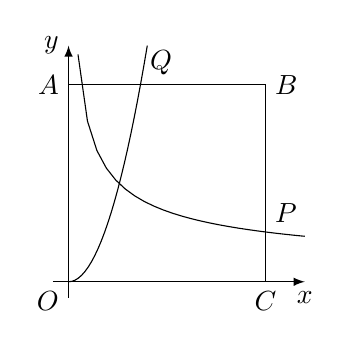
\begin{tikzpicture}[>=latex]
\draw [->] (-0.2,0) -- (3,0) node [below] {$x$};
\draw [->] (0,-0.2) -- (0,3) node [left] {$y$};
\draw (0,0) node [below left] {$O$};
\draw (2.5,0) node [below] {$C$} coordinate (C);
\draw (2.5,2.5) node [right] {$B$} coordinate (B);
\draw (0,2.5) node [left] {$A$} coordinate (A);
\draw [domain = 0:1] plot (\x,{3*\x*\x});
\draw [domain = 0.12:3] plot (\x,{pow(\x,-1/2)});
\draw (C) -- (B) -- (A);
\draw ({sqrt(2.5/3)},2.5) node [above right] {$Q$};
\draw (2.5,{pow(2.5,-1/2)}) node [above right] {$P$};
\end{tikzpicture}
\end{center}


关联目标:

暂未关联目标



标签: 第二单元

答案: 暂无答案

解答或提示: 暂无解答与提示

使用记录:

20211228	2022届高三1班	\fcolorbox[rgb]{0,0,0}{1.000,0.228,0}{0.886}


出处: 2022届高三上学期测验卷11第10题
\item { (004486)}某温室大棚规定: 一天中, 从中午$12$点到第二天上午$8$点为保温时段, 其余$4$小时为工人作业时段. 从中午$12$点连续测量$20$小时, 得出此温室大棚的温度$y$(单位: 度)与时间$t$(单位: 小时, $t\in [0,20]$)近似地满足函数$y=|t-13|+\dfrac b{t+2}$关系, 其中, $b$为大棚内一天中保温时段的通风量.\\
(1) 若一天中保温时段的通风量保持$100$个单位不变, 求大棚一天中保温时段的最低温度(精确到$0.1^\circ\text{C}$);\\
(2) 若要保持大棚一天中保温时段的最低温度不小于$17^\circ\text{C}$, 求大棚一天中保温时段通风量的最小值.


关联目标:

暂未关联目标



标签: 第二单元

答案: 暂无答案

解答或提示: 暂无解答与提示

使用记录:

20211116	2022届高三1班	\fcolorbox[rgb]{0,0,0}{1.000,0.078,0}{0.961}	\fcolorbox[rgb]{0,0,0}{1.000,0.180,0}{0.910}


出处: 2022届高三上学期测验卷07第19题
\item { (004496)}已知函数$y=f(x)$存在反函数$y=f^{-1}(x)$, 若函数$y=f(x)+2^x$的图像经过点$(1,4)$, 则函数$y=f^{-1}(x)+\log_2x$的图像必过点\blank{50}.


关联目标:

暂未关联目标



标签: 第二单元

答案: 暂无答案

解答或提示: 暂无解答与提示

使用记录:

20211123	2022届高三1班	\fcolorbox[rgb]{0,0,0}{1.000,0.000,0}{1.000}


出处: 2022届高三上学期测验卷08第8题
\item { (004500)}对于定义域为$D$的函数$f(x)$, 若存在$x_1,x_2\in D$且$x_1\ne x_2$, 使得$f(x_1^2)=f(x_2^2)=2f(x_1+x_2)$, 则称函数$f(x)$具有性质$M$. 若函数$g(x)=|\log_2x-1|$, $x\in (0,a]$具有性质$M$, 则实数$a$的最小值为\blank{50}.


关联目标:

暂未关联目标



标签: 第二单元

答案: 暂无答案

解答或提示: 暂无解答与提示

使用记录:

20211123	2022届高三1班	\fcolorbox[rgb]{0,0,0}{0.286,1.000,0}{0.143}


出处: 2022届高三上学期测验卷08第12题
\item { (004509)}若存在常数$k$($k>0$), 使得对定义域$D$内的任意$x_1$、$x_2$($x_1\ne x_2$), 都有$|f(x_1)-f(x_2)|\le k|x_1-x_2|$成立, 则称函数$f(x)$在其定义域$D$是``$k-$利普希兹条件函数''.\\
(1) 若函数$f(x)=\sqrt x$($1\le x\le 4$)是``$k-$利普希兹条件函数'', 求常数$k$的取值范围;\\
(2) 判断函数$f(x)=\log_2x$是否是``$2-$利普希兹条件函数'', 若是, 请证明, 若不是, 请说明理由;\\
(3) 若$y=f(x)$($x\in \mathbf{R}$)是周期为2的``$1-$利普希兹条件函数'', 证明: 对任意的实数$x_1$、$x_2$, 都有$|f(x_1)-f(x_2)|\le 1$.


关联目标:

暂未关联目标



标签: 第二单元

答案: 暂无答案

解答或提示: 暂无解答与提示

使用记录:

20211123	2022届高三1班	\fcolorbox[rgb]{0,0,0}{1.000,0.108,0}{0.946}	\fcolorbox[rgb]{0,0,0}{1.000,0.310,0}{0.845}	\fcolorbox[rgb]{0,0,0}{0.756,1.000,0}{0.378}


出处: 2022届高三上学期测验卷08第21题
\item { (004516)}函数$f(x)=1+\log_2x$($x\ge 4$)的反函数的定义域为\blank{50}.


关联目标:

暂未关联目标



标签: 第二单元

答案: 暂无答案

解答或提示: 暂无解答与提示

使用记录:

20211129	2022届高三1班	\fcolorbox[rgb]{0,0,0}{1.000,0.000,0}{1.000}


出处: 2022届高三上学期测验卷09第7题
\item { (004520)}设函数$f(x)=|x-a|-\dfrac 2x+a$, 若关于$x$的方程$f(x)=1$有且仅有两个不同的实数根, 则实数$a$的取值构成的集合为\blank{50}.


关联目标:

暂未关联目标



标签: 第二单元

答案: 暂无答案

解答或提示: 暂无解答与提示

使用记录:

暂无使用记录


出处: 2022届高三上学期测验卷09第11题
\item { (004523)}已知函数$f^{-1}(x)$为函数$f(x)$的反函数, 且函数$f(x-1)$的图像经过点$(1,1)$, 则函数$f^{-1}(x)$的图像一定经过点\bracket{20}
\fourch{$(0,1)$}{$(1,0)$}{$(1,2)$}{$(2,1)$}


关联目标:

暂未关联目标



标签: 第二单元

答案: 暂无答案

解答或提示: 暂无解答与提示

使用记录:

20211129	2022届高三1班	\fcolorbox[rgb]{0,0,0}{1.000,0.046,0}{0.977}


出处: 2022届高三上学期测验卷09第14题
\item { (004525)}已知函数$f(x)=\begin{cases} x^2, & x\text{为无理数}, \\ x, &x\text{为有理数},   \end{cases}$ 则以下$4$个命题:
\textcircled{1} $f(x)$是偶函数; \textcircled{2} $f(x)$在$[0,+\infty)$上是增函数; \textcircled{3} $f(x)$的值域为$\mathbf{R}$; \textcircled{4} 对于任意的正有理数$a$, $g(x)=f(x)-a$存在奇数个零点.
其中正确命题的个数为\bracket{20}.
\fourch{$0$}{$1$}{$2$}{$3$}


关联目标:

暂未关联目标



标签: 第二单元

答案: 暂无答案

解答或提示: 暂无解答与提示

使用记录:

20211129	2022届高三1班	\fcolorbox[rgb]{0,0,0}{1.000,0.326,0}{0.837}


出处: 2022届高三上学期测验卷09第16题
\item { (004530)}已知函数$f(x)$的定义域是$D$, 若对于任意的$x_1,x_2\in D$, 当$x_1<x_2$时, 都有$f(x_1)\le f(x_2)$, 则称函数$f(x)$在$D$上为``非减函数''.\\
(1) 判断$f_1(x)=x^2-4x, \ x\in [1,4]$与$f_2(x)=|x-1|+|x-2|, \ x\in [1,4]$是否是``非减函数''?\\
(2) 已知函数$g(x)=2^x+\dfrac a{2^{x-1}}$在$[2,4]$上为``非减函数'', 求实数$a$的取值范围;\\
(3) 已知函数$h(x)$在$[0,1]$上为``非减函数'', 且满足条件:
\textcircled{1}  $h(0)=0$; \textcircled{2}  $h(\dfrac x3)=\dfrac 12h(x)$; \textcircled{3}  $h(1-x)=1-h(x)$, 求 $h(\dfrac 1{2020})$的值.


关联目标:

暂未关联目标



标签: 第二单元

答案: 暂无答案

解答或提示: 暂无解答与提示

使用记录:

暂无使用记录


出处: 2022届高三上学期测验卷09第21题
\item { (004540)}已知$y=f(x)$是定义在$\mathbf{R}$上的奇函数, 且当$x\ge 0$时, $f(x)=-\dfrac 1{4^x}+\dfrac 1{2^x}$, 则此函数的值域为\blank{50}.


关联目标:

暂未关联目标



标签: 第二单元

答案: 暂无答案

解答或提示: 暂无解答与提示

使用记录:

20211214	2022届高三1班	\fcolorbox[rgb]{0,0,0}{1.000,0.232,0}{0.884}


出处: 2022届高三上学期测验卷10第10题
\item { (004542)}已知$p$是实数, 函数$f(x)=10^x$. 若存在实数$m,n$, 使得$f(m+n)=f(m)+f(n)$与$f(m+n+p)=f(m)+f(n)+f(p)$均成立, 则$p$的最大值等于\blank{50}.


关联目标:

暂未关联目标



标签: 第二单元

答案: 暂无答案

解答或提示: 暂无解答与提示

使用记录:

20211214	2022届高三1班	\fcolorbox[rgb]{0,0,0}{0.930,1.000,0}{0.465}


出处: 2022届高三上学期测验卷10第12题
\item { (004544)}设函数$f(x)=\begin{cases}1, & x\in \mathbf{Q}, \\ \pi, &x\not\in \mathbf{Q}.\end{cases}$ 下列结论不正确的是\bracket{20}.
\twoch{$f(x)$是偶函数}{$f(x)$是周期函数}{该函数有最大值也有最小值}{方程$f(f(x))=1$的解集为$\{1\}$}


关联目标:

暂未关联目标



标签: 第二单元

答案: 暂无答案

解答或提示: 暂无解答与提示

使用记录:

20211214	2022届高三1班	\fcolorbox[rgb]{0,0,0}{1.000,0.140,0}{0.930}


出处: 2022届高三上学期测验卷10第14题
\item { (004546)}若直线$y=kx+1$与曲线$y=|x+\dfrac 1x|-|x-\dfrac 1x|$有且仅有四个不同的交点, 则实数$k$的取值范围为\bracket{20}.
\fourch{$\{-\dfrac 18,0,\dfrac 18\}$}{$\{-\dfrac 18,\dfrac 18\}$}{$[-\dfrac 18,\dfrac 18]$}{$(-\dfrac 18,\dfrac 18)$}


关联目标:

暂未关联目标



标签: 第二单元

答案: 暂无答案

解答或提示: 暂无解答与提示

使用记录:

20211214	2022届高三1班	\fcolorbox[rgb]{0,0,0}{1.000,0.698,0}{0.651}


出处: 2022届高三上学期测验卷10第16题
\item { (004549)}某省4A级风景区内居住着一个少数民族村, 该村投资了$800$万元修复和加强民俗文化基础设施. 据调查, 修复好村民俗文化基础设施后, 任何一个月内(每月按$30$天计)每天的旅游人数$f(x)$与第$x$天近似地满足$f(x)=8+\dfrac 9x$(千人), 且参观民俗文化村的游客人均消费$g(x)$近似地满足$g(x)=143-|x-22|$(元).\\
(1) 求该村第$x$天的旅游收入$p(x)$(单位千元, $1\le x\le 30,x\in \mathbf{N}^*$)的函数关系;\\
(2) 若以最低日收入的$20\%$作为每一天的纯收入的计量依据, 并以纯收入的$5\%$的比例收回投资成本, 试问该村在两年内能否收回全部投资成本?


关联目标:

暂未关联目标



标签: 第二单元

答案: 暂无答案

解答或提示: 暂无解答与提示

使用记录:

20211214	2022届高三1班	\fcolorbox[rgb]{0,0,0}{1.000,0.224,0}{0.888}	\fcolorbox[rgb]{0,0,0}{1.000,0.430,0}{0.785}


出处: 2022届高三上学期测验卷10第19题
\item { (004555)}函数$f(x)=x^2$($x<0$)的反函数为\blank{50}.


关联目标:

暂未关联目标



标签: 第二单元

答案: 暂无答案

解答或提示: 暂无解答与提示

使用记录:

20211228	2022届高三1班	\fcolorbox[rgb]{0,0,0}{1.000,0.410,0}{0.795}


出处: 2022届高三上学期测验卷11第4题
\item { (004563)}下列函数中, 值域为$[0,+\infty)$的是\bracket{20}.
\fourch{$y=2^x$}{$y=x^\frac 12$}{$y=\tan x$}{$y=\cos x$}


关联目标:

暂未关联目标



标签: 第二单元

答案: 暂无答案

解答或提示: 暂无解答与提示

使用记录:

20211228	2022届高三1班	\fcolorbox[rgb]{0,0,0}{1.000,0.000,0}{1.000}


出处: 2022届高三上学期测验卷11第13题
\item { (004569)}改革开放$40$年, 我国卫生事业取得巨大成就, 卫生总费用增长了数十倍. 卫生总费用包括个人现在支出、社会支出、政府支出, 如表为$2012$年至$2015$年我国卫生费用中个人现金支出、社会支出和政府支出的费用(单位:亿元)和在卫生总费用中的占比. 
\begin{center}
    \begin{tabular}{|p{.05\textwidth}<\centering|p{.1\textwidth}<\centering|p{.1\textwidth}<\centering|p{.1\textwidth}<\centering|p{.1\textwidth}<\centering|p{.1\textwidth}<\centering|p{.1\textwidth}<\centering|p{.1\textwidth}<\centering|}
        \hline
         & & \multicolumn{2}{c|}{个人现金卫生支出} & \multicolumn{2}{c|}{社会卫生支出} & \multicolumn{2}{c|}{政府卫生支出} \\ \hline
         年份& 卫生总费用(亿元)& 绝对数(亿元) & 占卫生总费用比重($\%$) & 绝对数(亿元) & 占卫生总费用比重($\%$)& 绝对数(亿元) & 占卫生总费用比重($\%$)\\ \hline
        $2012$ & $28119.00$ & $9656.32$ & $34.34$ & $10030.70$ & $35.67$ & $8431.98$ & $29.99$ \\ \hline
        $2013$ & $31668.95$ & $10729.34$ & $33.88$ & $11393.79$ & $35.98$ & $9545.81$ & $30.14$ \\ \hline
        $2014$ & $35312.40$ & $11295.41$ & $31.99$ & $13437.75$ & $38.05$ & $10579.23$ & $29.96$ \\ \hline
        $2015$ & $40974.64$ & $11992.65$ & $29.27$ & $16506.71$ & $40.29$ & $12475.28$ & $30.45$ \\ \hline
    \end{tabular}
\end{center}
(数据来源于国家统计年鉴)\\
(1) 指出$2012$年到$2015$年之间我国卫生总费用中个人现金支出占比和社会支出占比的变化趋势;\\
(2) 设$t=1$表示$1978$年, 第$t$年卫生总费用与年份$t$之间拟合函数$f(t)=\dfrac{357876.6053}{1+\mathrm{e}^{6.4420-0.1136t}}$, 研究函数$f(t)$的单调性, 并预测我国卫生总费用首次超过$12$万亿的年份.


关联目标:

暂未关联目标



标签: 第二单元

答案: 暂无答案

解答或提示: 暂无解答与提示

使用记录:

20211228	2022届高三1班	\fcolorbox[rgb]{0,0,0}{1.000,0.220,0}{0.890}	\fcolorbox[rgb]{0,0,0}{1.000,0.386,0}{0.807}


出处: 2022届高三上学期测验卷11第19题
\item { (004620)}已知函数$f(x)=\lg (x+1)$的反函数为$y=f^{-1}(x)$, 则$f^{-1}(2)=$\blank{50}.


关联目标:

暂未关联目标



标签: 第二单元

答案: 暂无答案

解答或提示: 暂无解答与提示

使用记录:

20210924	2022届高三1班	\fcolorbox[rgb]{0,0,0}{1.000,0.000,0}{1.000}

20210924	2022届高三	\fcolorbox[rgb]{0,0,0}{1.000,0.052,0}{0.974}


出处: 2022届高三上月考卷01第2题
\item { (004622)}若$f(x)$是奇函数, 且当$x\ge 0$时, $f(x)=x^2+x$, 则当$x<0$时, $f(x)=$\blank{50}.


关联目标:

暂未关联目标



标签: 第二单元

答案: 暂无答案

解答或提示: 暂无解答与提示

使用记录:

20210924	2022届高三1班	\fcolorbox[rgb]{0,0,0}{1.000,0.182,0}{0.909}

20210924	2022届高三	\fcolorbox[rgb]{0,0,0}{1.000,0.206,0}{0.897}


出处: 2022届高三上月考卷01第4题
\item { (004636)}已知$a$是常数, 设函数$f(x)=(a-2)x^2+2(a-2)x-4$.\\
(1) 解不等式: $f(x)>-4$;\\
(2) 求实数$a$的取值范围, 使得$f(x)<0$对任意$x\in [1,3]$恒成立;


关联目标:

K0115001B|D01004B|能通过对判别式讨论的方法解决含参一元二次(可能是一元一次, 可能不含未知数)不等式的恒成立问题.

K0114001B|D01004B|掌握结合一元二次函数的图像求解一元二次不等式的方法.



标签: 第一单元|第二单元

答案: 暂无答案

解答或提示: 暂无解答与提示

使用记录:

20210924	2022届高三1班	\fcolorbox[rgb]{0,0,0}{1.000,0.318,0}{0.841}	\fcolorbox[rgb]{0,0,0}{1.000,0.120,0}{0.940}

20210924	2022届高三	\fcolorbox[rgb]{0,0,0}{1.000,0.380,0}{0.810}	\fcolorbox[rgb]{0,0,0}{1.000,0.248,0}{0.876}


出处: 2022届高三上月考卷01第18题
\item { (004640)}方程$2^x=3$的解为$x=$\blank{50}.


关联目标:

暂未关联目标



标签: 第二单元

答案: 暂无答案

解答或提示: 暂无解答与提示

使用记录:

20211209	2022届高三1班	\fcolorbox[rgb]{0,0,0}{1.000,0.000,0}{1.000}

20211209	2022届高三	\fcolorbox[rgb]{0,0,0}{1.000,0.000,0}{1.000}


出处: 2022届高三上月考卷02第1题
\item { (004649)}已知$f(x)=m(x-2m)(x+m+3)$, $g(x)=2^x-2$, 满足对于任意的$x\in \mathbf{R}$, $f(x)<0$或$g(x)<0$, 则$m$的取值范围是\blank{50}.


关联目标:

暂未关联目标



标签: 第二单元

答案: 暂无答案

解答或提示: 暂无解答与提示

使用记录:

20211209	2022届高三1班	\fcolorbox[rgb]{0,0,0}{1.000,0.636,0}{0.682}

20211209	2022届高三	\fcolorbox[rgb]{0,0,0}{1.000,0.932,0}{0.534}


出处: 2022届高三上月考卷02第10题
\item { (004658)}如图, $A$、$B$、$C$三地有直道相通, $AB=5$千米, $AC=3$千米, $BC=4$千米, 现甲、乙两警员同时从$A$地出发匀速前往$B$地, 经过$t$小时, 他们之间的距离为$f(t)$(单位: 千米), 甲的路线是$AB$, 速度为$5$千米/小时, 乙的路线是$ACB$, 速度为$8$千米/小时, 乙到$B$地后在原地等待, 设$t=t_1$时乙到达$C$地.
\begin{center}
    \begin{tikzpicture}[scale = 0.6]
        \draw (0,0) node [left] {$C$} -- (4,0) node [right] {$B$} -- (0,3) node [above] {$A$} -- cycle;
    \end{tikzpicture}
\end{center}
(1) 求$t_1$及$f(t_1)$的值;\\
(2) 已知警员的对讲机的有效通话距离是$3$千米, 当$t_1\le t\le 1$时, 求$f(t)$的表达式, 并判断$f(t)$在$[t_1,1]$上的最大值是否超过$3$? 说明理由.


关联目标:

暂未关联目标



标签: 第二单元

答案: 暂无答案

解答或提示: 暂无解答与提示

使用记录:

20211209	2022届高三1班	\fcolorbox[rgb]{0,0,0}{1.000,0.106,0}{0.947}	\fcolorbox[rgb]{0,0,0}{1.000,0.454,0}{0.773}

20211209	2022届高三	\fcolorbox[rgb]{0,0,0}{1.000,0.300,0}{0.850}	\fcolorbox[rgb]{0,0,0}{1.000,0.832,0}{0.584}


出处: 2022届高三上月考卷02第19题
\item { (004661)}函数$f(x)={x^{-\frac 12}}$的定义域是\blank{50}.


关联目标:

暂未关联目标



标签: 第二单元

答案: 暂无答案

解答或提示: 暂无解答与提示

使用记录:

20211109	2022届高三	\fcolorbox[rgb]{0,0,0}{1.000,0.060,0}{0.970}


出处: 2022届高三上期中区统考第1题
\item { (004665)}方程$\lg (x+2)=2\lg x$的解为\blank{50}.


关联目标:

暂未关联目标



标签: 第二单元

答案: 暂无答案

解答或提示: 暂无解答与提示

使用记录:

20211109	2022届高三	\fcolorbox[rgb]{0,0,0}{1.000,0.006,0}{0.997}


出处: 2022届高三上期中区统考第5题
\item { (004667)}若函数$f(x)=\sqrt{2x+1}$的反函数为$g(x)$, 则函数$g(x)$的零点为\blank{50}.


关联目标:

暂未关联目标



标签: 第二单元

答案: 暂无答案

解答或提示: 暂无解答与提示

使用记录:

20211109	2022届高三	\fcolorbox[rgb]{0,0,0}{1.000,0.458,0}{0.771}


出处: 2022届高三上期中区统考第7题
\item { (004671)}设$f(x)$是定义在$\mathbf{R}$上的函数, 且满足$f(1)=0$.若$y=f(x)+a\cdot 2^x$是奇函数, $y=f(x)+3^x$是偶函数, 则$a$的值为\blank{50}.


关联目标:

暂未关联目标



标签: 第二单元

答案: 暂无答案

解答或提示: 暂无解答与提示

使用记录:

20211109	2022届高三	\fcolorbox[rgb]{0,0,0}{1.000,0.402,0}{0.799}


出处: 2022届高三上期中区统考第11题
\item { (004679)}为实现``碳达峰'', 减少污染, 某化工企业开发了一个废料回收项目. 经测算, 该项目日回收成本$p$(元)与日回收量$x$(吨)($x\in [0,50]$)的函数关系可表示为$p=\begin{cases}20x, & 0\le x\le 30,  \\ x^2+16x-780, & 30<x \le 50,  \end{cases}$ 且每回收$1$吨废料, 转化成其他产品可收入$80$元.\\
(1) 设日纯收益为$y$元, 写出函数$y=f(x)$的解析式(纯收益$=$收入$-$成本);\\
(2) 该公司每日回收废料多少吨时, 获得纯收益最大?


关联目标:

暂未关联目标



标签: 第二单元

答案: 暂无答案

解答或提示: 暂无解答与提示

使用记录:

20211109	2022届高三	\fcolorbox[rgb]{0,0,0}{1.000,0.050,0}{0.975}	\fcolorbox[rgb]{0,0,0}{1.000,0.168,0}{0.916}


出处: 2022届高三上期中区统考第19题
\item { (004680)}已知函数$f(x)=2^x+\dfrac a{2^x}$, $a$为实常数.\\
(1) 若函数$f(x)$为奇函数, 求$a$的值;\\
(2) 若$x\in [0,1]$时$f(x)$的最小值为$2$, 求$a$的值;\\
(3) 若方程$f(x)=6$有两个不等的实根$x_1,x_2$, 且$|x_1-x_2|\le 1$, 求$a$的取值范围.


关联目标:

暂未关联目标



标签: 第二单元

答案: 暂无答案

解答或提示: 暂无解答与提示

使用记录:

20211109	2022届高三	\fcolorbox[rgb]{0,0,0}{1.000,0.234,0}{0.883}	\fcolorbox[rgb]{0,0,0}{1.000,0.340,0}{0.830}	\fcolorbox[rgb]{0,0,0}{1.000,0.906,0}{0.547}


出处: 2022届高三上期中区统考第20题
\item { (004684)}已知函数$f(x)=\dfrac{x-1}{x+2}$的反函数为$f^{-1}(x)$, 则$f^{-1}(0)=$\blank{50}.


关联目标:

暂未关联目标



标签: 第二单元

答案: 暂无答案

解答或提示: 暂无解答与提示

使用记录:

20211221	2022届高三	\fcolorbox[rgb]{0,0,0}{1.000,0.066,0}{0.967}


出处: 2022届高三上一模第3题
\item { (004689)}方程$\log_3(x^2-1)=2+\log_3(x-1)$的解为$x=$\blank{50}.


关联目标:

暂未关联目标



标签: 第二单元

答案: 暂无答案

解答或提示: 暂无解答与提示

使用记录:

20211221	2022届高三	\fcolorbox[rgb]{0,0,0}{1.000,0.024,0}{0.988}


出处: 2022届高三上一模第8题
\item { (004702)}给定区间$I$和正常数$a$, 如果定义在$\mathbf{R}$上的两个函数$y=f(x)$与$y=g(x)$满足: 对一切$x\in I$, 均有$|f(x)-g(x)|\le a$, 称函数$y=f(x)$与$y=g(x)$具有性质$P(I,a)$.\\
(1)	已知$I=(0,+\infty)$, 判断下列两组函数是否具有性质$P(I,2)$? \textcircled{1} $f_1(x)=\dfrac 1{{x^2}+1}$, $g_1(x)=2$; \textcircled{2} $f_2(x)=x^2+x+1$, $g_2(x)=x^2-x+1$;(不需要说明理由)\\
(2)	已知$f(x)=0$, $y=g(x)$是周期函数, 且对任意的$a>0$, 均存在区间$I=(M,+\infty)$, 使得函数$y=f(x)$与$y=g(x)$具有性质$P(I,a)$, 求证: $g(x)=0$;\\
(3)	已知$I=[1,m]$, $f(x)=x^2$, 若存在一次函数$y=g(x)$与$y=f(x)$具有性质$P(I,1)$, 求实数$m$的最大值.


关联目标:

暂未关联目标



标签: 第二单元

答案: 暂无答案

解答或提示: 暂无解答与提示

使用记录:

20211221	2022届高三	\fcolorbox[rgb]{0,0,0}{1.000,0.026,0}{0.987}	\fcolorbox[rgb]{0,0,0}{0.398,1.000,0}{0.199}	\fcolorbox[rgb]{0,0,0}{0.062,1.000,0}{0.031}


出处: 2022届高三上一模第21题
\item { (004704)}函数$y=\log_2(x+1)$的反函数为\blank{50}.


关联目标:

暂未关联目标



标签: 第二单元

答案: 暂无答案

解答或提示: 暂无解答与提示

使用记录:

20220414	2022届高三	\fcolorbox[rgb]{0,0,0}{1.000,0.036,0}{0.982}


出处: 2022届高三下期中区统考第2题
\item { (004720)}已知函数$f(x)=x^2+mx+3$, 其中$m\in \mathbf{R}$.\\
(1) 若不等式$f(x)<5$的解集是$(-1,2)$, 求$m$的值;\\
(2) 若函数$y=f(x)$在区间$[0,3]$上有且仅有一个零点, 求$m$的取值范围.


关联目标:

暂未关联目标



标签: 第二单元

答案: 暂无答案

解答或提示: 暂无解答与提示

使用记录:

20220414	2022届高三	\fcolorbox[rgb]{0,0,0}{1.000,0.042,0}{0.979}	\fcolorbox[rgb]{0,0,0}{1.000,0.670,0}{0.665}


出处: 2022届高三下期中区统考第18题
\item { (004721)}如图, 有一块扇形草地$OMN$, 已知半径为$4$, $\angle MON=\dfrac\pi 2$, 现要在其中圈出一块举行场地$ABCD$作为儿童乐园使用, 其中点$A$、$B$在弧$\overset\frown{MN}$上, 且线段$AB$平行于线段$MN$.
\begin{center}
    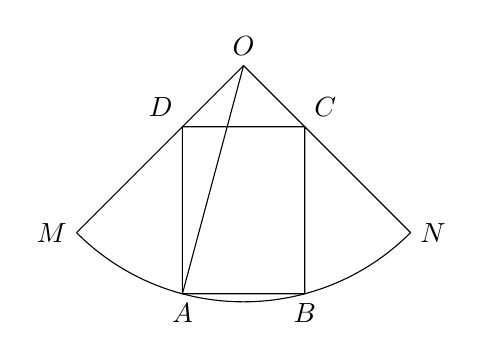
\begin{tikzpicture}[scale = 1.5]
        \draw (0,0) node [above] {$O$} coordinate (O);
        \draw (-45:2) node [right] {$N$} coordinate (N);
        \draw (-135:2) node [left] {$M$} coordinate (M);
        \draw (-75:2) node [below] {$B$} coordinate (B);
        \draw (-105:2) node [below] {$A$} coordinate (A);
        \draw (-45:{2/sin(45)*sin(15)}) node [above right] {$C$} coordinate (C);
        \draw (-135:{2/sin(45)*sin(15)}) node [above left] {$D$} coordinate (D);
        \draw (M) -- (O) -- (N) (A) rectangle (C) (O) -- (A);
        \draw (M) arc (-135:-45:2);
    \end{tikzpicture}
\end{center}
(1) 若点$A$为弧$\overset\frown{MN}$的一个三等分点, 求矩形$ABCD$的面积$S$;\\
(2) 当$A$在何处时, 矩形$ABCD$的面积$S$最大? 最大值为多少?


关联目标:

暂未关联目标



标签: 第二单元

答案: 暂无答案

解答或提示: 暂无解答与提示

使用记录:

20220414	2022届高三	\fcolorbox[rgb]{0,0,0}{1.000,0.302,0}{0.849}	\fcolorbox[rgb]{0,0,0}{1.000,0.652,0}{0.674}


出处: 2022届高三下期中区统考第19题
\item { (004729)}函数$f(x)=1+\lg x$的反函数是$f^{-1}(x)$=\blank{50}.


关联目标:

暂未关联目标



标签: 第二单元

答案: 暂无答案

解答或提示: 暂无解答与提示

使用记录:

20220621	2022届高三	\fcolorbox[rgb]{0,0,0}{1.000,0.128,0}{0.936}


出处: 2022届高三下二模第6题
\item { (004731)}已知集合$A=\{-2,-1,-\dfrac 12,\dfrac 13,\dfrac 12,1,2,3\}$, 从集合$A$中任取一个元素$a$, 使函数$y=x^a$是奇函数且在$(0,+\infty)$上递增的概率为\blank{50}.


关联目标:

暂未关联目标



标签: 第二单元|第八单元

答案: 暂无答案

解答或提示: 暂无解答与提示

使用记录:

20220621	2022届高三	\fcolorbox[rgb]{0,0,0}{1.000,0.230,0}{0.885}


出处: 2022届高三下二模第8题
\item { (004739)}对于定义在集合$D$上的两个函数$y_1=f_1(x)$与$y_2=f_2(x)$, 若对任意的$x\in D$, 总有$|f_2(x)|\le |f_1(x)|$成立, 则称函数$f_1(x)$包裹函数$f_2(x)$. 判断如下两个命题真假:\\
\textcircled{1}  函数$f_1(x)=kx$包裹函数$f_2(x)=x\cos x$的充要条件是$|k|\ge 1$;
\textcircled{2}  若对于任意$p>0$, $|f_1(x)-f_2(x)|<p$对任意$x\in D$都成立, 则函数$f_1(x)$包裹函数$f_2(x)$;\\
则下列选项正确的是\bracket{20}.
\fourch{\textcircled{1} 真, \textcircled{2} 假}{\textcircled{1} 假, \textcircled{2} 真}{\textcircled{1}、\textcircled{2} 全假}{\textcircled{1}、\textcircled{2} 全真}


关联目标:

暂未关联目标



标签: 第二单元

答案: 暂无答案

解答或提示: 暂无解答与提示

使用记录:

20220621	2022届高三	\fcolorbox[rgb]{0,0,0}{0.612,1.000,0}{0.306}


出处: 2022届高三下二模第16题
\item { (004755)}设$y=f^{-1}(x)$是函数$f(x)=\dfrac x2+\dfrac{\pi}8\sin x+\dfrac{\pi}8$, $x\in [-\dfrac{\pi }2,\dfrac{\pi }2]$的反函数, 则函数$y=f(x)+f^{-1}(x)$的最小值等于\blank{50}.


关联目标:

暂未关联目标



标签: 第二单元|第三单元

答案: 暂无答案

解答或提示: 暂无解答与提示

使用记录:

20220317	2022届高三1班	\fcolorbox[rgb]{0,0,0}{1.000,0.884,0}{0.558}


出处: 2022届高三下月考卷01第11题
\item { (004756)}函数$f(x)=x$, $g(x)=x^2-x+2$. 若存在$x_1, x_2,\cdots,x_n\in [0,\dfrac 92]$, 使得$f(x_1)+f(x_2)+...+f(x_{n-1})+g(x_n)=g(x_1)+g(x_2)+...+g(x_{n-1})+f(x_n)$, 则$n$的最大值为\blank{50}.


关联目标:

暂未关联目标



标签: 第二单元

答案: 暂无答案

解答或提示: 暂无解答与提示

使用记录:

20220317	2022届高三1班	\fcolorbox[rgb]{0,0,0}{1.000,0.744,0}{0.628}


出处: 2022届高三下月考卷01第12题
\item { (004757)}下列函数中既是奇函数, 又在区间$(0,+\infty)$上单调递减的函数为\bracket{20}.
\fourch{$y=\sqrt x$}{$y=\log_{\frac 12}x$}{$y=-x^3$}{$y=x+\dfrac 1x$}


关联目标:

暂未关联目标



标签: 第二单元

答案: 暂无答案

解答或提示: 暂无解答与提示

使用记录:

20220317	2022届高三1班	\fcolorbox[rgb]{0,0,0}{1.000,0.000,0}{1.000}


出处: 2022届高三下月考卷01第13题
\item { (004760)}已知以下三个陈述句:\\
$p$: 存在$a\in \mathbf{R}$且$a\ne 0$, 对任意的$x\in \mathbf{R}$, 均有$f(2^{x+a})<f(2^x)+f(a)$恒成立;\\
$q_1$: 函数$y=f(x)$是定义域为$\mathbf{R}$的减函数, 且对任意的$x\in \mathbf{R}$, 都有$f(x)>0$;\\
$q_2$: 函数$y=f(x)$是定义域为$\mathbf{R}$的增函数, 存在$x_0<0$, 使得$f(x_0)=0$;\\
用这三个陈述句组成两个命题, 命题$S$: ``若$q_1$, 则$p$''; 命题$T$: ``若$q_2$, 则$p$''. 关于$S,T$以下说法正确的是\bracket{20}.
\twoch{只有命题$S$是真命题}{只有命题$T$是真命题}{两个命题$S,T$都是真命题}{两个命题$S,T$都不是真命题}


关联目标:

暂未关联目标



标签: 第二单元

答案: 暂无答案

解答或提示: 暂无解答与提示

使用记录:

20220317	2022届高三1班	\fcolorbox[rgb]{0,0,0}{1.000,0.466,0}{0.767}


出处: 2022届高三下月考卷01第16题
\item { (004763)}新冠肺炎疫情造成医用防护服紧缺, 某地政府决定为防护服生产企业A公司扩大生产提供$x$($x\in [0,10]$)(万元)的专项补贴, 并以每套$80$元的价格收购其生产的全部防护服. $A$公司在收到政府$x$(万元)补贴后, 防护服产量将增加到$t=k\cdot (6-\dfrac{12}{x+4})$(万套), 其中$k$为工厂工人的复工率($k\in [0.5,1]$). $A$公司生产$t$万件防护服还需投入成本$20+8x+50t$(万元).\\
(1) 将$A$公司生产防护服的利润$y$(万元)表示为补贴$x$(万元)的函数(利润不包含政府补贴);\\
(2) 若对任意的$x\in [0,10]$(万元), $A$公司都不会产生亏损, 求复工率$k$的取值范围.


关联目标:

暂未关联目标



标签: 第二单元

答案: 暂无答案

解答或提示: 暂无解答与提示

使用记录:

20220317	2022届高三1班	\fcolorbox[rgb]{0,0,0}{1.000,0.186,0}{0.907}	\fcolorbox[rgb]{0,0,0}{1.000,0.220,0}{0.890}


出处: 2022届高三下月考卷01第19题
\item { (004909)}设$a>0$, $a\ne 1$, $t>0$, 比较$\dfrac 12\log_at$和$\log_a\dfrac{t+1}2$的大小.


关联目标:

K0111003B|D01003B|会用不等式的性质、作差法证明一些简单的不等式.



标签: 第一单元|第二单元

答案: 暂无答案

解答或提示: 暂无解答与提示

使用记录:

暂无使用记录


出处: 代数精编第二章不等式
\item { (004980)}记$f(x)=x^2+ax+b$, 求证: $|f(1)|,|f(2)|,|f(3)|$中至少有一个不小于$\dfrac 12$.


关联目标:

K0107003B|D01002B|了解反证法的思想以及表达方式, 能正确使用反证法证明一些简单的数学命题.



标签: 第一单元|第二单元

答案: 暂无答案

解答或提示: 暂无解答与提示

使用记录:

暂无使用记录


出处: 代数精编第二章不等式
\item { (004981)}已知$-1\le x\le 1$, $n\ge 2$, $n\in \mathbf{N}$, 求证: $(1-x)^n+(1+x)^n\le 2^n$.


关联目标:

K0408002X|D04004X|知道数学归纳法是一种证明与自然数有关的命题的方法, 理解数学归纳法的基本原理.

K0408003X|D04004X|初步掌握数学归纳法证明与自然数有关命题的一般步骤, 会用数学归纳法证明一些与自然数有关的一些简单等式.



标签: 第一单元|第二单元

答案: 暂无答案

解答或提示: 暂无解答与提示

使用记录:

暂无使用记录


出处: 代数精编第二章不等式
\item { (004995)}从半径为$R$的圆形铁片里剪去一个扇形, 然后把剩下部分卷成一个圆锥形漏斗, 要使漏斗有最大容量, 剪去扇形的圆心角$\theta$应是多少弧度?


关联目标:

K0119001B|D01003B|会运用平均值不等式求解较简单的最大值和最小值问题.



标签: 第一单元|第二单元

答案: 暂无答案

解答或提示: 暂无解答与提示

使用记录:

暂无使用记录


出处: 代数精编第二章不等式
\item { (005012)}若$a>1$, $b>1$, $c>1$, 则$\log_ab+\log_ba$的最小值为\blank{50}, $\log_ab+\log_bc+\log_ca$的最小值为\blank{50}.


关联目标:

K0119001B|D01003B|会运用平均值不等式求解较简单的最大值和最小值问题.



标签: 第一单元|第二单元

答案: 暂无答案

解答或提示: 暂无解答与提示

使用记录:

暂无使用记录


出处: 代数精编第二章不等式
\item { (005036)}利用$a^2+b^2+c^2\ge ab+bc+ca(a,b,c\in \mathbf{R})$, 证明: 若$a,b,c>0$, $n\in \mathbf{N}$, $f(n)=\lg \dfrac{a^n+b^n+c^n}3$, 则$2f(n)\le f(2n)$.


关联目标:

K0118003B|D01003B|能运用平均值不等式比较大小、证明一些简单的不等式.



标签: 第一单元|第二单元

答案: 暂无答案

解答或提示: 暂无解答与提示

使用记录:

暂无使用记录


出处: 代数精编第二章不等式
\item { (005038)}利用放缩法并结合公式$ab\le (\dfrac{a+b}2)^2$, 证明: $\log_a(a-1)\cdot \log_a(a+1)<1$($a>1$).


关联目标:

K0118003B|D01003B|能运用平均值不等式比较大小、证明一些简单的不等式.



标签: 第一单元|第二单元

答案: 暂无答案

解答或提示: 暂无解答与提示

使用记录:

暂无使用记录


出处: 代数精编第二章不等式
\item { (005052)}利用函数的单调性证明: 若$x>0$, $y>0$, $x+y=1$, 则$(x+\dfrac 1x)(y+\dfrac 1y)\ge \dfrac{25}4$.


关联目标:

暂未关联目标



标签: 第一单元|第二单元

答案: 暂无答案

解答或提示: 暂无解答与提示

使用记录:

暂无使用记录


出处: 代数精编第二章不等式
\item { (005053)}利用函数的单调性证明: 若$0<a<\dfrac 1k(k\ge 2,k\in \mathbf{N})$, 且$a^2<a-b$, 则$b<\dfrac 1{k+1}$.


关联目标:

暂未关联目标



标签: 第一单元|第二单元

答案: 暂无答案

解答或提示: 暂无解答与提示

使用记录:

暂无使用记录


出处: 代数精编第二章不等式
\item { (005085)}已知$f(x)=\lg \dfrac{1+2^x+a\cdot 4^x}3$($a\in \mathbf{R}$).\\
(1) 如果$x\le 1$时$f(x)$有意义, 求$a$的取值范围;\\
(2) 如果$0<a\le 1$, 求证: $x\ne 0$时, $2f(x)<f(2x)$.


关联目标:

暂未关联目标



标签: 第二单元

答案: 暂无答案

解答或提示: 暂无解答与提示

使用记录:

暂无使用记录


出处: 代数精编第二章不等式
\item { (005086)}求证: $2+\sin \theta +\cos \theta \ge \dfrac 2{2-\sin \theta -\cos \theta }$.


关联目标:

暂未关联目标



标签: 第二单元|第三单元

答案: 暂无答案

解答或提示: 暂无解答与提示

使用记录:

暂无使用记录


出处: 代数精编第二章不等式
\item { (005087)}求证: $-1<\dfrac{4\sin \theta +3}{\sin^2\theta+1}\le 4$.


关联目标:

暂未关联目标



标签: 第二单元|第三单元

答案: 暂无答案

解答或提示: 暂无解答与提示

使用记录:

暂无使用记录


出处: 代数精编第二章不等式
\item { (005089)}求证: $2\sin 2\alpha \le \cot \dfrac{\alpha}2$, 其中$0<\alpha <\pi$.


关联目标:

暂未关联目标



标签: 第二单元|第三单元

答案: 暂无答案

解答或提示: 暂无解答与提示

使用记录:

暂无使用记录


出处: 代数精编第二章不等式
\item { (005090)}求证: 若$x>-1$, 则$(\dfrac 13)^{x+\frac 32}<(\dfrac 13)^{\sqrt{(x+1)(x+2)}}$.


关联目标:

暂未关联目标



标签: 第二单元

答案: 暂无答案

解答或提示: 暂无解答与提示

使用记录:

暂无使用记录


出处: 代数精编第二章不等式
\item { (005093)}求证: 若$x>y>0$, $\theta \in (0,\dfrac{\pi}2)$, 则$x\sec \theta -y\tan \theta \ge \sqrt{x^2-y^2}$.


关联目标:

暂未关联目标



标签: 第二单元|第三单元

答案: 暂无答案

解答或提示: 暂无解答与提示

使用记录:

暂无使用记录


出处: 代数精编第二章不等式
\item { (005095)}求证: $16^{18}>18^{16}$.


关联目标:

暂未关联目标



标签: 第二单元

答案: 暂无答案

解答或提示: 暂无解答与提示

使用记录:

暂无使用记录


出处: 代数精编第二章不等式
\item { (005096)}求证: $(\sqrt 2)^{\sqrt 3}<(\sqrt 3)^{\sqrt 2}$.


关联目标:

暂未关联目标



标签: 第二单元

答案: 暂无答案

解答或提示: 暂无解答与提示

使用记录:

暂无使用记录


出处: 代数精编第二章不等式
\item { (005103)}下列函数中, 最小值为$2$的是\bracket{20}.
\twoch{$x+\dfrac 1x$}{$\dfrac{x^2+2}{\sqrt{x^2+1}}$}{$\log_ax+\log_xa$($a>0$, $x>0$, $a\ne 1$, $x\ne 1$)}{$3^x+3^{-x}$($x>0$)}


关联目标:

暂未关联目标



标签: 第一单元|第二单元

答案: 暂无答案

解答或提示: 暂无解答与提示

使用记录:

暂无使用记录


出处: 代数精编第二章不等式
\item { (005104)}若$\log_{\sqrt 2}x+\log_{\sqrt 2}y=4$, 则$x+y$的最小值是\bracket{20}.
\fourch{$8$}{$4\sqrt 2$}{$4$}{$2$}


关联目标:

暂未关联目标



标签: 第一单元|第二单元

答案: 暂无答案

解答或提示: 暂无解答与提示

使用记录:

暂无使用记录


出处: 代数精编第二章不等式
\item { (005105)}若$a,b$均为大于$1$的正数, 且$ab=100$, 则$\lg a\cdot \lg b$的最大值是\bracket{20}.
\fourch{$0$}{$1$}{$2$}{$\dfrac 52$}


关联目标:

暂未关联目标



标签: 第一单元|第二单元

答案: 暂无答案

解答或提示: 暂无解答与提示

使用记录:

暂无使用记录


出处: 代数精编第二章不等式
\item { (005110)}若$x+2y=2\sqrt 2a$($x>0$, $y>0$, $a>1$), 则$\log_ax+\log_ay$的最大值是\blank{50}.


关联目标:

暂未关联目标



标签: 第一单元|第二单元

答案: 暂无答案

解答或提示: 暂无解答与提示

使用记录:

暂无使用记录


出处: 代数精编第二章不等式
\item { (005118)}若正数$x,y,z$满足$5x+2y+z=100$, 则$\lg x+\lg y+\lg z$的最大值是\blank{50}.


关联目标:

暂未关联目标



标签: 第一单元|第二单元

答案: 暂无答案

解答或提示: 暂无解答与提示

使用记录:

暂无使用记录


出处: 代数精编第二章不等式
\item { (005124)}求函数$y=\dfrac{x^4+3x^2+3}{x^2+1}$的最小值.


关联目标:

暂未关联目标



标签: 第二单元

答案: 暂无答案

解答或提示: 暂无解答与提示

使用记录:

暂无使用记录


出处: 代数精编第二章不等式
\item { (005125)}求$f(x)=4x^2+\dfrac{16}{(x^2+1)^2}$的最小值.


关联目标:

暂未关联目标



标签: 第二单元

答案: 暂无答案

解答或提示: 暂无解答与提示

使用记录:

暂无使用记录


出处: 代数精编第二章不等式
\item { (005126)}求$f(x)=x^2-3x-2-\dfrac 3x+\dfrac 1{x^2}$($x>0$)的最小值.


关联目标:

暂未关联目标



标签: 第二单元

答案: 暂无答案

解答或提示: 暂无解答与提示

使用记录:

暂无使用记录


出处: 代数精编第二章不等式
\item { (005132)}已知函数$f(x)=\dfrac{2^{x+3}}{{4^x}+8}$.\\
(1) 求$f(x)$的最大值;\\
(2) 对于任意实数$a,b$, 求证: $f(a)<b^2-4b+\dfrac{11}2$.


关联目标:

暂未关联目标



标签: 第一单元|第二单元

答案: 暂无答案

解答或提示: 暂无解答与提示

使用记录:

暂无使用记录


出处: 代数精编第二章不等式
\item { (005136)}在$\triangle ABC$中, 已知$BC=a$, $CA=b$, $AB=c$, $\angle ACB=\theta$. 现将$\triangle ABC$分别以$BC,CA,AB$所在直线为轴旋转一周, 设所得三个旋转体的体积依次为$V_1,V_2,V_3$.\\
(1) 设$T=\dfrac{V_3}{V_1+V_2}$, 试用$a,b,c$表示$T$;\\
(2) 若$\theta$为定值, 并令$\dfrac{a+b}c=x$, 将$T=\dfrac{V_3}{V_1+V_2}$表示为$x$的函数, 写出这个函数的定义域, 并求这个函数的最大值$M$;\\
(3) 若$\theta \in [\dfrac{\pi }3,\pi)$, 求(2)中$M$的最大值.


关联目标:

暂未关联目标



标签: 第一单元|第二单元

答案: 暂无答案

解答或提示: 暂无解答与提示

使用记录:

暂无使用记录


出处: 代数精编第二章不等式
\item { (005146)}解关于$x$的不等式$|\log_ax|<|\log_a(ax^2)|-2$($0<a<1$).


关联目标:

暂未关联目标



标签: 第一单元|第二单元

答案: 暂无答案

解答或提示: 暂无解答与提示

使用记录:

暂无使用记录


出处: 代数精编第二章不等式
\item { (005193)}$\lg x^2<2$的解集是\bracket{20}.
\twoch{$\{x|-10<x<0\text{或}0<x<10\}$}{$\{x|x<10\}$}{$\{x|0<x<10\}$}{$\{x|-10<x<10\}$}


关联目标:

暂未关联目标



标签: 第二单元

答案: 暂无答案

解答或提示: 暂无解答与提示

使用记录:

暂无使用记录


出处: 代数精编第二章不等式
\item { (005194)}若$f(x)=\log_2x$, 则不等式$[f(x)]^2>f(x^2)$的解集是\bracket{20}.
\fourch{$\{x|0<x<\dfrac 14\}$}{$\{x|\dfrac 14<x<1\}$}{$\{x|0<x<1\text{或}x>4\}$}{$\{x|\dfrac 14<x<4\}$}


关联目标:

暂未关联目标



标签: 第二单元

答案: 暂无答案

解答或提示: 暂无解答与提示

使用记录:

暂无使用记录


出处: 代数精编第二章不等式
\item { (005195)}若$a,b$都是小于$1$的正数, 且$a^{\log_b(x-5)}<1$, 则$x$的取值范围是\bracket{20}.
\fourch{$x>5$}{$x<6$}{$5<x<6$}{$x<5$或$x>6$}


关联目标:

暂未关联目标



标签: 第二单元

答案: 暂无答案

解答或提示: 暂无解答与提示

使用记录:

暂无使用记录


出处: 代数精编第二章不等式
\item { (005196)}不等式$\log_x\dfrac 45<1$的解集是\bracket{20}.
\twoch{$\{x|0<x<\dfrac 45\}$}{$\{x|x>\dfrac 45\}$}{$\{x|\dfrac 45<x<1\}$}{$\{x|0<x<\dfrac 45\}\cup \{x|x>1\}$}


关联目标:

暂未关联目标



标签: 第二单元

答案: 暂无答案

解答或提示: 暂无解答与提示

使用记录:

暂无使用记录


出处: 代数精编第二章不等式
\item { (005197)}若函数$f(x)=\log_{a^2-1}(2x+1)$在区间$(-\dfrac 12,0)$内恒有$f(x)>0$, 则实数$a$的取值范围是\bracket{20}.
\twoch{$0<a<1$}{$a>1$}{$-\sqrt 2<a<-1$或$1<a<\sqrt 2$}{$a<-\sqrt 2$或$a>\sqrt 2$}


关联目标:

暂未关联目标



标签: 第二单元

答案: 暂无答案

解答或提示: 暂无解答与提示

使用记录:

暂无使用记录


出处: 代数精编第二章不等式
\item { (005198)}若不等式$\log_a(x^2-2x+3)\le -1$对一切实数都成立, 则$a$的取值范围是\bracket{20}.
\fourch{$a\ge 2$}{$1<a\le 2$}{$\dfrac 12\le a<1$}{$0<a\le \dfrac 12$}


关联目标:

暂未关联目标



标签: 第二单元

答案: 暂无答案

解答或提示: 暂无解答与提示

使用记录:

暂无使用记录


出处: 代数精编第二章不等式
\item { (005200)}解关于$x$的不等式: $\log_{\frac 13}(x^2-x-2)>\log_{\frac 13}(2x^2-7x+3)$.


关联目标:

暂未关联目标



标签: 第二单元

答案: 暂无答案

解答或提示: 暂无解答与提示

使用记录:

暂无使用记录


出处: 代数精编第二章不等式
\item { (005201)}解关于$x$的不等式: $\log_x\dfrac 12<1$.


关联目标:

暂未关联目标



标签: 第二单元

答案: 暂无答案

解答或提示: 暂无解答与提示

使用记录:

暂无使用记录


出处: 代数精编第二章不等式
\item { (005202)}解关于$x$的不等式: $\lg (x-\dfrac 1x)<0$.


关联目标:

暂未关联目标



标签: 第二单元

答案: 暂无答案

解答或提示: 暂无解答与提示

使用记录:

暂无使用记录


出处: 代数精编第二章不等式
\item { (005203)}解关于$x$的不等式: $\log_2|x-\dfrac 12|<-1$.


关联目标:

暂未关联目标



标签: 第二单元

答案: 暂无答案

解答或提示: 暂无解答与提示

使用记录:

暂无使用记录


出处: 代数精编第二章不等式
\item { (005204)}已知集合$M=\{x|\log_3(x-m)>1\}$与$P=\{x|3^{5-3x} \ge \dfrac 13\}$满足$M\cap P\ne \varnothing$, 求实数$m$的取值范围.


关联目标:

暂未关联目标



标签: 第二单元

答案: 暂无答案

解答或提示: 暂无解答与提示

使用记录:

暂无使用记录


出处: 代数精编第二章不等式
\item { (005205)}解不等式: $\log_8(2-x)+\log_{64}(x+1)\ge \log_4x$.


关联目标:

暂未关联目标



标签: 第二单元

答案: 暂无答案

解答或提示: 暂无解答与提示

使用记录:

暂无使用记录


出处: 代数精编第二章不等式
\item { (005206)}解不等式: $\log_{0.5}(x+13)<\log_{0.5}(x^2-2x-15)$.


关联目标:

暂未关联目标



标签: 第二单元

答案: 暂无答案

解答或提示: 暂无解答与提示

使用记录:

暂无使用记录


出处: 代数精编第二章不等式
\item { (005207)}解不等式: $\log_x(3\sqrt{x-1}-1)>1$.


关联目标:

暂未关联目标



标签: 第二单元

答案: 暂无答案

解答或提示: 暂无解答与提示

使用记录:

暂无使用记录


出处: 代数精编第二章不等式
\item { (005208)}解不等式: $\log_{x-1}(6-x-x^2)>2$.


关联目标:

暂未关联目标



标签: 第二单元

答案: 暂无答案

解答或提示: 暂无解答与提示

使用记录:

暂无使用记录


出处: 代数精编第二章不等式
\item { (005209)}解不等式: $\dfrac 1{\log_2(x-1)}<\dfrac 1{\log_2\sqrt{x+1}}$.


关联目标:

暂未关联目标



标签: 第二单元

答案: 暂无答案

解答或提示: 暂无解答与提示

使用记录:

暂无使用记录


出处: 代数精编第二章不等式
\item { (005210)}解不等式: $\dfrac{\log_3(1-\dfrac{3x}2)}{\log_9(2x)}\ge 1$.


关联目标:

暂未关联目标



标签: 第二单元

答案: 暂无答案

解答或提示: 暂无解答与提示

使用记录:

暂无使用记录


出处: 代数精编第二章不等式
\item { (005211)}解不等式: $\log_{0.5}({2^x}-1)\cdot \log_{0.5}({2^{x-1}}-\dfrac 12)\le 2$.


关联目标:

暂未关联目标



标签: 第二单元

答案: 暂无答案

解答或提示: 暂无解答与提示

使用记录:

暂无使用记录


出处: 代数精编第二章不等式
\item { (005212)}解关于$x$的不等式, 其中$a>0$, $a\ne 1$: $\log_a(x+1-a)>1$.


关联目标:

暂未关联目标



标签: 第二单元

答案: 暂无答案

解答或提示: 暂无解答与提示

使用记录:

暂无使用记录


出处: 代数精编第二章不等式
\item { (005213)}解关于$x$的不等式, 其中$a>0$, $a\ne 1$: $\log_a(1-\dfrac 1x)>1$.


关联目标:

暂未关联目标



标签: 第二单元

答案: 暂无答案

解答或提示: 暂无解答与提示

使用记录:

暂无使用记录


出处: 代数精编第二章不等式
\item { (005214)}解关于$x$的不等式, 其中$a>0$, $a\ne 1$: $\log_a(2x-1)>\log_a(x-1)$.


关联目标:

暂未关联目标



标签: 第二单元

答案: 暂无答案

解答或提示: 暂无解答与提示

使用记录:

暂无使用记录


出处: 代数精编第二章不等式
\item { (005215)}解关于$x$的不等式, 其中$a>0$, $a\ne 1$: $\log_a^2x<\log_x^2a$.


关联目标:

暂未关联目标



标签: 第二单元

答案: 暂无答案

解答或提示: 暂无解答与提示

使用记录:

暂无使用记录


出处: 代数精编第二章不等式
\item { (005216)}解关于$x$的不等式, 其中$a>0$, $a\ne 1$: ${x^{\log_ax}}>\dfrac{x^4\cdot \sqrt x}{a^2}$.


关联目标:

暂未关联目标



标签: 第二单元

答案: 暂无答案

解答或提示: 暂无解答与提示

使用记录:

暂无使用记录


出处: 代数精编第二章不等式
\item { (005217)}解关于$x$的不等式, 其中$a>0$, $a\ne 1$: $\sqrt{\log_ax-1}>3-\log_ax$.


关联目标:

暂未关联目标



标签: 第二单元

答案: 暂无答案

解答或提示: 暂无解答与提示

使用记录:

暂无使用记录


出处: 代数精编第二章不等式
\item { (005218)}已知$x$满足不等式$(\dfrac 12)^{2x-4}-(\dfrac 12)^x-(\dfrac 12)^{x-2}+\dfrac 14\le 0$, 且$y=\log_{\frac 1a}(a^2x)\cdot \log_{\frac 1{a^2}}(ax)$的最大值是$0$, 最小值是$-\dfrac 18$, 求实数$a$的值.


关联目标:

暂未关联目标



标签: 第二单元

答案: 暂无答案

解答或提示: 暂无解答与提示

使用记录:

暂无使用记录


出处: 代数精编第二章不等式
\item { (005219)}已知关于$x$的方程$x^2-5x\log_ak+6\log _a^2k=0$的两根中$(k>1)$, 仅较小的根在区间$(1,2)$内, 试用$a$表示$k$的取值范围($a>0$且$a\ne 1$).


关联目标:

暂未关联目标



标签: 第二单元

答案: 暂无答案

解答或提示: 暂无解答与提示

使用记录:

暂无使用记录


出处: 代数精编第二章不等式
\item { (005231)}解不等式: $\log_2|x-\dfrac 12|<-1$.


关联目标:

暂未关联目标



标签: 第二单元

答案: 暂无答案

解答或提示: 暂无解答与提示

使用记录:

暂无使用记录


出处: 代数精编第二章不等式
\item { (005232)}若函数$y=\log_ax$在$x\in [2,+\infty)$上恒有$|y|>1$, 则实数$a$的取值范围是\blank{50}.


关联目标:

暂未关联目标



标签: 第二单元

答案: 暂无答案

解答或提示: 暂无解答与提示

使用记录:

暂无使用记录


出处: 代数精编第二章不等式
\item { (005240)}解不等式: $\log_{\frac 14}|x|<\log_{\frac 12}|x+1|$.


关联目标:

暂未关联目标



标签: 第二单元

答案: 暂无答案

解答或提示: 暂无解答与提示

使用记录:

暂无使用记录


出处: 代数精编第二章不等式
\item { (005241)}解不等式: $|\lg (1-x)|>|\lg (1+x)|$.


关联目标:

暂未关联目标



标签: 第二单元

答案: 暂无答案

解答或提示: 暂无解答与提示

使用记录:

暂无使用记录


出处: 代数精编第二章不等式
\item { (005242)}解不等式: $|\log_{\frac 13}x|+|\log_{\frac 13}\dfrac 1{3-x}|\ge 1$.


关联目标:

暂未关联目标



标签: 第二单元

答案: 暂无答案

解答或提示: 暂无解答与提示

使用记录:

暂无使用记录


出处: 代数精编第二章不等式
\item { (005243)}求函数$f(x)=|x-\dfrac 12|-|x+\dfrac 12|$的最大值.


关联目标:

暂未关联目标



标签: 第二单元

答案: 暂无答案

解答或提示: 暂无解答与提示

使用记录:

暂无使用记录


出处: 代数精编第二章不等式
\item { (005244)}已知$|\lg x-\lg y|\le 1$, 则$\dfrac xy+\dfrac yx$的取值范围是\blank{50}.


关联目标:

暂未关联目标



标签: 第二单元

答案: 暂无答案

解答或提示: 暂无解答与提示

使用记录:

暂无使用记录


出处: 代数精编第二章不等式
\item { (005245)}解关于$x$的不等式: $|\log_{\sqrt a}x-2|-|\log_ax-2|<2$.


关联目标:

暂未关联目标



标签: 第二单元

答案: 暂无答案

解答或提示: 暂无解答与提示

使用记录:

暂无使用记录


出处: 代数精编第二章不等式
\item { (005246)}解关于$x$的不等式: $|\log_ax|<|\log_a(ax^2)|-2$.


关联目标:

暂未关联目标



标签: 第二单元

答案: 暂无答案

解答或提示: 暂无解答与提示

使用记录:

暂无使用记录


出处: 代数精编第二章不等式
\item { (005247)}解关于$x$的不等式: $|3^x-3|+9^x-3>0$.


关联目标:

暂未关联目标



标签: 第二单元

答案: 暂无答案

解答或提示: 暂无解答与提示

使用记录:

暂无使用记录


出处: 代数精编第二章不等式
\item { (005248)}解关于$x$的不等式: $|a^x-1|+|a^{2x}-3|>2(a>0)$.


关联目标:

暂未关联目标



标签: 第二单元

答案: 暂无答案

解答或提示: 暂无解答与提示

使用记录:

暂无使用记录


出处: 代数精编第二章不等式
\item { (005253)}已知常数$a\in (0,1)$, 对任意$x>0$, $f(\log_ax)=\dfrac{a(x^2-1)}{x(a^2-1)}$.\\
(l) 求$f(x)$($x\in \mathbf{R}$)的表达式, 并判断它的单调性;\\
(2) 若$n\ge 2$, $n\in \mathbf{N}$, 求证: $f(n)>n$.


关联目标:

暂未关联目标



标签: 第二单元

答案: 暂无答案

解答或提示: 暂无解答与提示

使用记录:

暂无使用记录


出处: 代数精编第二章不等式
\item { (005263)}解不等式: $2^{x+1}+x>0$.


关联目标:

暂未关联目标



标签: 第二单元

答案: 暂无答案

解答或提示: 暂无解答与提示

使用记录:

暂无使用记录


出处: 代数精编第二章不等式
\item { (005272)}求函数$y=\dfrac{3x-1}{x+1}$的值域.


关联目标:

暂未关联目标



标签: 第二单元

答案: 暂无答案

解答或提示: 暂无解答与提示

使用记录:

暂无使用记录


出处: 代数精编第三章函数
\item { (005273)}求函数$y=\dfrac{4x+3}{2x-1}$的值域.


关联目标:

暂未关联目标



标签: 第二单元

答案: 暂无答案

解答或提示: 暂无解答与提示

使用记录:

暂无使用记录


出处: 代数精编第三章函数
\item { (005274)}求函数$y=\dfrac{x^2-1}{x^2+2}$的值域.


关联目标:

暂未关联目标



标签: 第二单元

答案: 暂无答案

解答或提示: 暂无解答与提示

使用记录:

暂无使用记录


出处: 代数精编第三章函数
\item { (005275)}求函数$y=\dfrac{x^2-x+1}{2x^2-2x+3}$的值域.


关联目标:

暂未关联目标



标签: 第二单元

答案: 暂无答案

解答或提示: 暂无解答与提示

使用记录:

暂无使用记录


出处: 代数精编第三章函数
\item { (005276)}求函数$y=\dfrac{x^2+4x+3}{x^2+x-6}$的值域.


关联目标:

暂未关联目标



标签: 第二单元

答案: 暂无答案

解答或提示: 暂无解答与提示

使用记录:

暂无使用记录


出处: 代数精编第三章函数
\item { (005277)}若实数$x,y$满足$x^2+4y^2=4x$, 求$S=x^2+y^2$的值域.


关联目标:

暂未关联目标



标签: 第二单元

答案: 暂无答案

解答或提示: 暂无解答与提示

使用记录:

暂无使用记录


出处: 代数精编第三章函数
\item { (005278)}已知函数$y=f(x)=x^2+ax+3$在区间$x\in [-1,1]$上的最小值为$-3$, 求实数$a$的值.


关联目标:

暂未关联目标



标签: 第二单元

答案: 暂无答案

解答或提示: 暂无解答与提示

使用记录:

暂无使用记录


出处: 代数精编第三章函数
\item { (005279)}求函数$y=3x^2-12x+18\sqrt {4x-x^2}-23$的值域.


关联目标:

暂未关联目标



标签: 第二单元

答案: 暂无答案

解答或提示: 暂无解答与提示

使用记录:

暂无使用记录


出处: 代数精编第三章函数
\item { (005280)}求函数$y=|x-2|-|x+1|$的值域.


关联目标:

暂未关联目标



标签: 第二单元

答案: 暂无答案

解答或提示: 暂无解答与提示

使用记录:

暂无使用记录


出处: 代数精编第三章函数
\item { (005281)}若$f(x-1)=2x^2+1$, 求$f(x)$.


关联目标:

暂未关联目标



标签: 第二单元

答案: 暂无答案

解答或提示: 暂无解答与提示

使用记录:

暂无使用记录


出处: 代数精编第三章函数
\item { (005282)}已知定义域为$\mathbf{R}$的函数$f(x)$满足:
\textcircled{1} $f(x+y)=f(x)\cdot f(y)$对任何实数$x,y$都成立;
\textcircled{2} 存在实数$x_1,x_2$, 使$f(x_1)\ne f(x_2)$.
求证:\\
(1) $f(0)=1$;\\
(2) $f(x)>0$.


关联目标:

暂未关联目标



标签: 第二单元

答案: 暂无答案

解答或提示: 暂无解答与提示

使用记录:

暂无使用记录


出处: 代数精编第三章函数
\item { (005283)}设映射$f:X\to Y$, 其中$X,Y$是非空集合, 则下列语句中正确的是\bracket{20}.
\twoch{$Y$中每一个元素必有原像}{$Y$中的各元素只能有一个原像}{$X$中的不同元素在$Y$中的像也不同}{$Y$中至少存在一个元素, 它有原像}


关联目标:

暂未关联目标



标签: 第二单元

答案: 暂无答案

解答或提示: 暂无解答与提示

使用记录:

暂无使用记录


出处: 代数精编第三章函数
\item { (005284)}集合$M=\{a,b,c\}$与$P=\{x,y,z\}$之间建立起四种对应关系(如图), 则下列结论中正确的是\bracket{20}.
\begin{center}
    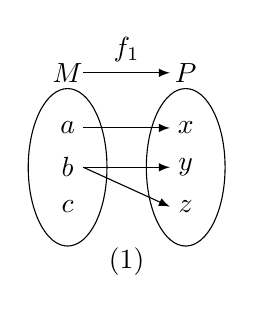
\begin{tikzpicture}[>=latex]
        \draw (0,0) ellipse (0.5 and 1);
        \draw (0,0.5) node {$a$} (0,0) node {$b$} (0,-0.5) node {$c$};
        \draw (1.5,0) ellipse (0.5 and 1);
        \draw (1.5,0.5) node {$x$} (1.5,0) node {$y$} (1.5,-0.5) node {$z$};
        \draw [->] (0.2,0.5) -- (1.3,0.5);
        \draw [->] (0.2,0) -- (1.3,0);
        \draw [->] (0.2,0) -- (1.3,-0.5);
        \draw [->] (0.2,1.2) -- (1.3,1.2);
        \draw (0,1.2) node {$M$} (1.5,1.2) node{$P$};
        \draw (0.75,1.5) node {$f_1$} (0.75,-1.2) node {(1)};
    \end{tikzpicture}
    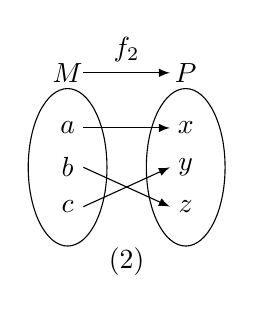
\begin{tikzpicture}[>=latex]
      \draw (0,0) ellipse (0.5 and 1);
      \draw (0,0.5) node {$a$} (0,0) node {$b$} (0,-0.5) node {$c$};
      \draw (1.5,0) ellipse (0.5 and 1);
      \draw (1.5,0.5) node {$x$} (1.5,0) node {$y$} (1.5,-0.5) node {$z$};
      \draw [->] (0.2,0.5) -- (1.3,0.5);
      \draw [->] (0.2,0) -- (1.3,-0.5);
      \draw [->] (0.2,-0.5) -- (1.3,0);
      \draw [->] (0.2,1.2) -- (1.3,1.2);
      \draw (0,1.2) node {$M$} (1.5,1.2) node{$P$};
      \draw (0.75,1.5) node {$f_2$} (0.75,-1.2) node {(2)};
  \end{tikzpicture}
  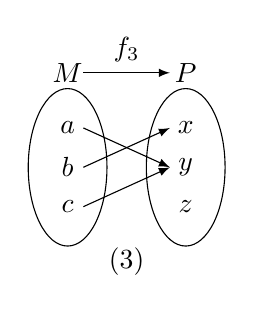
\begin{tikzpicture}[>=latex]
    \draw (0,0) ellipse (0.5 and 1);
    \draw (0,0.5) node {$a$} (0,0) node {$b$} (0,-0.5) node {$c$};
    \draw (1.5,0) ellipse (0.5 and 1);
    \draw (1.5,0.5) node {$x$} (1.5,0) node {$y$} (1.5,-0.5) node {$z$};
    \draw [->] (0.2,0.5) -- (1.3,0);
    \draw [->] (0.2,0) -- (1.3,0.5);
    \draw [->] (0.2,-0.5) -- (1.3,0);
    \draw [->] (0.2,1.2) -- (1.3,1.2);
    \draw (0,1.2) node {$M$} (1.5,1.2) node{$P$};
    \draw (0.75,1.5) node {$f_3$} (0.75,-1.2) node {(3)};
\end{tikzpicture}
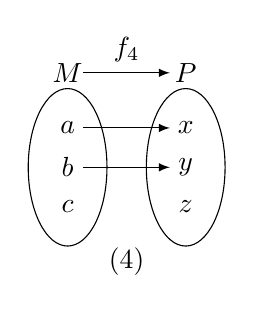
\begin{tikzpicture}[>=latex]
  \draw (0,0) ellipse (0.5 and 1);
  \draw (0,0.5) node {$a$} (0,0) node {$b$} (0,-0.5) node {$c$};
  \draw (1.5,0) ellipse (0.5 and 1);
  \draw (1.5,0.5) node {$x$} (1.5,0) node {$y$} (1.5,-0.5) node {$z$};
  \draw [->] (0.2,0.5) -- (1.3,0.5);
  \draw [->] (0.2,0) -- (1.3,0);
  \draw [->] (0.2,1.2) -- (1.3,1.2);
  \draw (0,1.2) node {$M$} (1.5,1.2) node{$P$};
  \draw (0.75,1.5) node {$f_4$} (0.75,-1.2) node {(4)};
\end{tikzpicture}
\end{center}
\twoch{只有$f_2,f_3$是从$M$到$P$的映射}{只有$f_2,f_4$是从$M$到$P$的映射}{只有$f_3,f_4$是从$M$到$P$的映射}{$f_1,f_2,f_3,f_4$都是从$M$到$P$的映射}


关联目标:

暂未关联目标



标签: 第二单元

答案: 暂无答案

解答或提示: 暂无解答与提示

使用记录:

暂无使用记录


出处: 代数精编第三章函数
\item { (005285)}设$(x,y)$在映射$f$下的像是$(\dfrac{x+y}2,\dfrac{x-y}2)$, 则在$f$下$(-5,2)$的原像是\bracket{20}.
\fourch{$(-10,4)$}{$(-3,-7)$}{$(-6,-4)$}{$(-\dfrac 32,-\dfrac 72)$}


关联目标:

暂未关联目标



标签: 第二单元

答案: 暂无答案

解答或提示: 暂无解答与提示

使用记录:

暂无使用记录


出处: 代数精编第三章函数
\item { (005286)}在给定的映射$f:(x,y)\mapsto (2x+y,xy)$($x,y\in \mathbf{R}$)下, 点$(\dfrac 16,-\dfrac 16)$的原像是\bracket{20}.
\fourch{$(\dfrac 16,-\dfrac 1{36})$}{$(\dfrac 13,-\dfrac 12)$或$(-\dfrac 14,\dfrac 23)$}{$(\dfrac 1{36},-\dfrac 16)$}{$(\dfrac 12,-\dfrac 13)$或$(-\dfrac 23,\dfrac 14)$}


关联目标:

暂未关联目标



标签: 第二单元

答案: 暂无答案

解答或提示: 暂无解答与提示

使用记录:

暂无使用记录


出处: 代数精编第三章函数
\item { (005287)}已知集合$M=\{x|0\le x\le 6\}$, $P=\{0\le y\le 3\}$, 则下列对应关系中, 不能作为从$M$到$P$的映射的是\bracket{20}.
\fourch{$f:x\mapsto y=\dfrac 12x$}{$f:x\mapsto y=\dfrac 13x$}{$f:x\mapsto y=x$}{$f:x\mapsto y=\dfrac 16x$}


关联目标:

暂未关联目标



标签: 第二单元

答案: 暂无答案

解答或提示: 暂无解答与提示

使用记录:

暂无使用记录


出处: 代数精编第三章函数
\item { (005288)}设$M=\mathbf{R}$, 从$M$到$P$的映射$f:x\mapsto y=\dfrac 1{x^2+1}$, 则像集$P$为\bracket{20}.
\fourch{$\{y|y\in \mathbf{R}\}$}{$\{y|y\in \mathbf{R}\}$}{$\{y|0\le y\le 2\}$}{$\{y|0<y\le 1\}$}


关联目标:

暂未关联目标



标签: 第二单元

答案: 暂无答案

解答或提示: 暂无解答与提示

使用记录:

暂无使用记录


出处: 代数精编第三章函数
\item { (005289)}若映射$f:A\to B$的像集是$Y$, 原像的集合是$X$, 则$X$与$A$的关系是\blank{50}, $Y$和$B$的关系是\blank{50}.


关联目标:

暂未关联目标



标签: 第二单元

答案: 暂无答案

解答或提示: 暂无解答与提示

使用记录:

暂无使用记录


出处: 代数精编第三章函数
\item { (005290)}若$(x,y)$在映射$f$下的像是$(2x-y,x+2y)$, 则$(-1,2)$在$f$下的原像是\blank{50}.


关联目标:

暂未关联目标



标签: 第二单元

答案: 暂无答案

解答或提示: 暂无解答与提示

使用记录:

暂无使用记录


出处: 代数精编第三章函数
\item { (005291)}已知$(a,b)$在映射$f$的像是$(a-b,ab)$, 则$(2,3)$的原像是\blank{50}.


关联目标:

暂未关联目标



标签: 第二单元

答案: 暂无答案

解答或提示: 暂无解答与提示

使用记录:

暂无使用记录


出处: 代数精编第三章函数
\item { (005292)}已知$f:x\mapsto y=x^2$是从集合$\mathbf{R}$到集合$M=\{x|x\ge 0\}$的一个映射, 则$M$中的元素$1$在$\mathbf{R}$中的原像是\blank{50}, $M$中的元素$t$($t>0$)在$\mathbf{R}$中的原像是\blank{50}.


关联目标:

暂未关联目标



标签: 第二单元

答案: 暂无答案

解答或提示: 暂无解答与提示

使用记录:

暂无使用记录


出处: 代数精编第三章函数
\item { (005293)}从集合$\{a\}$到$\{b,c\}$的不同映射有\blank{50}个.


关联目标:

暂未关联目标



标签: 第二单元

答案: 暂无答案

解答或提示: 暂无解答与提示

使用记录:

暂无使用记录


出处: 代数精编第三章函数
\item { (005294)}从集合$\{1,2\}$到$\{5,6\}$的不同映射有\blank{50}个.


关联目标:

暂未关联目标



标签: 第二单元

答案: 暂无答案

解答或提示: 暂无解答与提示

使用记录:

暂无使用记录


出处: 代数精编第三章函数
\item { (005295)}已知集合$A=\mathbf{Z}$, $B=\{x|x=2n+1, \ n\in \mathbf{Z}\}$, $C=\mathbf{R}$, 且从$A$到$B$的映射是$x\mapsto 2x-1$, 从$B$到$C$的映射是$x\mapsto \dfrac 1{3x+1}$, 则从$A$到$C$的映射是\blank{50}.


关联目标:

暂未关联目标



标签: 第二单元

答案: 暂无答案

解答或提示: 暂无解答与提示

使用记录:

暂无使用记录


出处: 代数精编第三章函数
\item { (005296)}$f$是集合$X=\{a,b,c\}$到集合$Y=\{d,e\}$的一个映射, 则满足映射条件的``$f$''共有\bracket{20}.
\fourch{$5$个}{$6$个}{$7$个}{$8$个}


关联目标:

暂未关联目标



标签: 第二单元

答案: 暂无答案

解答或提示: 暂无解答与提示

使用记录:

暂无使用记录


出处: 代数精编第三章函数
\item { (005297)}若$f:y=3x+1$是从集合$A=\{1,2,3,k\}$到集合$B=\{4,7,a^4,a^2+3a\}$的一个映射, 求自然数$a,k$的值及集合$A,B$.


关联目标:

暂未关联目标



标签: 第二单元

答案: 暂无答案

解答或提示: 暂无解答与提示

使用记录:

暂无使用记录


出处: 代数精编第三章函数
\item { (005298)}函数$f(x)=\dfrac{\sqrt{x^2-5x+6}}{x-2}$的定义域是\bracket{20}.
\fourch{$\{x|2<x<3\}$}{$\{x|x<2x>3\}$}{$\{x|x\le 2x\ge 3\}$}{$\{x|x<2\text{或}x\ge 3\}$}


关联目标:

暂未关联目标



标签: 第二单元

答案: 暂无答案

解答或提示: 暂无解答与提示

使用记录:

暂无使用记录


出处: 代数精编第三章函数
\item { (005299)}若函数$f(x)$的定义域是$[-1,1]$, 则函数$f(x+1)$的定义域是\bracket{20}.
\fourch{$[-1,1]$}{$[0,2]$}{$[-2,0]$}{$[0,1]$}


关联目标:

暂未关联目标



标签: 第二单元

答案: 暂无答案

解答或提示: 暂无解答与提示

使用记录:

暂无使用记录


出处: 代数精编第三章函数
\item { (005300)}在\textcircled{1} $y=x$与$y=\sqrt {x^2}$; \textcircled{2} $y=\sqrt {x^2}$与$y=(\sqrt x)^2$; \textcircled{3} $y=|x|$与$y=\dfrac{x^2}x$; \textcircled{4} $y=|x|$与$y=\sqrt {x^2}$; \textcircled{5} $y=x^0$与$y=1$这五组函数中, 表示同一函数的组数是\bracket{20}.
\fourch{$0$}{$1$}{$2$}{$3$}


关联目标:

暂未关联目标



标签: 第二单元

答案: 暂无答案

解答或提示: 暂无解答与提示

使用记录:

暂无使用记录


出处: 代数精编第三章函数
\item { (005301)}函数$y=-x^2-2x+3(-5\le x\le 0)$的值域是\bracket{20}.
\fourch{$(-\infty ,4]$}{$[3,12]$}{$[-12,4]$}{$[4,12]$}


关联目标:

暂未关联目标



标签: 第二单元

答案: 暂无答案

解答或提示: 暂无解答与提示

使用记录:

暂无使用记录


出处: 代数精编第三章函数
\item { (005302)}已知镭经过$100$年后剩下原来质量的$95.76\%$, 若质量为$l$克的镭经过$x$年后的剩余质量为$y$克, 则$y$与$x$之间的解析式是\bracket{20}.
\fourch{$y=(\dfrac{0.9576}{100})^x$}{$y=(0.9576)^{100x}$}{$y=(0.9576)^{\frac x{100}}$}{$y=1-(1-0.9576)^{\frac x{100}}$}


关联目标:

暂未关联目标



标签: 第二单元

答案: 暂无答案

解答或提示: 暂无解答与提示

使用记录:

暂无使用记录


出处: 代数精编第三章函数
\item { (005303)}函数$y=x+\dfrac{|x|}x$的图像是\bracket{20}.
\fourch{\begin{tikzpicture}[scale = 0.7,>=latex]
\draw [->] (-2,0) -- (2,0) node [below] {$x$};
\draw [->] (0,-2) -- (0,2) node [left] {$y$};
\draw (0,0) node [below right] {$O$};
\draw (-1,0) node [below] {$-1$} (0,1) node [right] {$1$};
\draw (-2,-1) -- (1,2);
\filldraw [white] (0,1) circle (0.05);
\draw (0,1) circle (0.05);
\end{tikzpicture}}{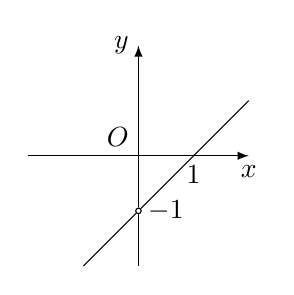
\begin{tikzpicture}[scale = 0.7,>=latex]
\draw [->] (-2,0) -- (2,0) node [below] {$x$};
\draw [->] (0,-2) -- (0,2) node [left] {$y$};
\draw (0,0) node [above left] {$O$};
\draw (1,0) node [below] {$1$} (0,-1) node [right] {$-1$};
\draw (-1,-2) -- (2,1);
\filldraw [white] (0,-1) circle (0.05);
\draw (0,-1) circle (0.05);
\end{tikzpicture}}{\begin{tikzpicture}[scale = 0.7,>=latex]
\draw [->] (-2,0) -- (2,0) node [below] {$x$};
\draw [->] (0,-2) -- (0,2) node [left] {$y$};
\draw (0,0) node [below right] {$O$};
\draw (1,0.1) -- (1,0) node [below] {$1$} (0,-1) node [right] {$-1$} (0,1) node [right] {$1$} (-1,0.1) -- (-1,0) node [below] {$-1$};
\draw (-1,-2) -- (0,-1) (0,1) -- (1,2);
\filldraw [white] (0,-1) circle (0.05);
\draw (0,-1) circle (0.05);
\filldraw [white] (0,1) circle (0.05);
\draw (0,1) circle (0.05);
\end{tikzpicture}}{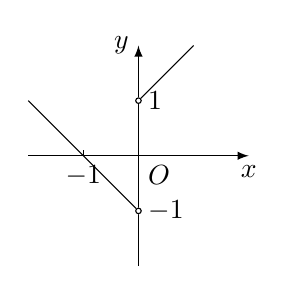
\begin{tikzpicture}[scale = 0.7,>=latex]
\draw [->] (-2,0) -- (2,0) node [below] {$x$};
\draw [->] (0,-2) -- (0,2) node [left] {$y$};
\draw (0,0) node [below right] {$O$};
\draw (0,-1) node [right] {$-1$} (0,1) node [right] {$1$} (-1,0.1) -- (-1,0) node [below] {$-1$};
\draw (-2,1) -- (0,-1) (0,1) -- (1,2);
\filldraw [white] (0,-1) circle (0.05);
\draw (0,-1) circle (0.05);
\filldraw [white] (0,1) circle (0.05);
\draw (0,1) circle (0.05);
\end{tikzpicture}}


关联目标:

暂未关联目标



标签: 第二单元

答案: 暂无答案

解答或提示: 暂无解答与提示

使用记录:

暂无使用记录


出处: 代数精编第三章函数
\item { (005304)}函数$y=\sqrt {1-x^2}+\sqrt {x+1}$的定义域为\blank{50}.


关联目标:

暂未关联目标



标签: 第二单元

答案: 暂无答案

解答或提示: 暂无解答与提示

使用记录:

暂无使用记录


出处: 代数精编第三章函数
\item { (005305)}函数$y=\dfrac 1{\sqrt {2x^2+3}}$的定义域为\blank{50}.


关联目标:

暂未关联目标



标签: 第二单元

答案: 暂无答案

解答或提示: 暂无解答与提示

使用记录:

暂无使用记录


出处: 代数精编第三章函数
\item { (005306)}函数$y=\dfrac{x+5}{3x^2-2x-1}$的定义域为\blank{50}.


关联目标:

暂未关联目标



标签: 第二单元

答案: 暂无答案

解答或提示: 暂无解答与提示

使用记录:

暂无使用记录


出处: 代数精编第三章函数
\item { (005307)}函数$y=\sqrt {6x-x^2-9}$的定义域为\blank{50}.


关联目标:

暂未关联目标



标签: 第二单元

答案: 暂无答案

解答或提示: 暂无解答与提示

使用记录:

暂无使用记录


出处: 代数精编第三章函数
\item { (005308)}函数$y=\sqrt {4-x^2}+\dfrac 1{|x|-1}$的定义域为\blank{50}.


关联目标:

暂未关联目标



标签: 第二单元

答案: 暂无答案

解答或提示: 暂无解答与提示

使用记录:

暂无使用记录


出处: 代数精编第三章函数
\item { (005309)}函数$y=\dfrac{x^3-1}{x+|x|}$的定义域为\blank{50}.


关联目标:

暂未关联目标



标签: 第二单元

答案: 暂无答案

解答或提示: 暂无解答与提示

使用记录:

暂无使用记录


出处: 代数精编第三章函数
\item { (005310)}函数$y=\dfrac 1{|x|-x^2}$的定义域为\blank{50}.


关联目标:

暂未关联目标



标签: 第二单元

答案: 暂无答案

解答或提示: 暂无解答与提示

使用记录:

暂无使用记录


出处: 代数精编第三章函数
\item { (005311)}函数$y=\sqrt {1-(\dfrac{x-1}{x+1})^2}$的定义域为\blank{50}.


关联目标:

暂未关联目标



标签: 第二单元

答案: 暂无答案

解答或提示: 暂无解答与提示

使用记录:

暂无使用记录


出处: 代数精编第三章函数
\item { (005312)}函数$y=\dfrac{\sqrt {x^2-2x-15}}{|x+3|-8}$的定义域为\blank{50}.


关联目标:

暂未关联目标



标签: 第二单元

答案: 暂无答案

解答或提示: 暂无解答与提示

使用记录:

暂无使用记录


出处: 代数精编第三章函数
\item { (005313)}函数$y=1-\dfrac 1{x+2}$的值域为\blank{50}.


关联目标:

暂未关联目标



标签: 第二单元

答案: 暂无答案

解答或提示: 暂无解答与提示

使用记录:

暂无使用记录


出处: 代数精编第三章函数
\item { (005314)}函数$y=\dfrac 3{2x}$的值域为\blank{50}.


关联目标:

暂未关联目标



标签: 第二单元

答案: 暂无答案

解答或提示: 暂无解答与提示

使用记录:

暂无使用记录


出处: 代数精编第三章函数
\item { (005315)}函数$y=\dfrac{x+3}{x-3}$的值域为\blank{50}.


关联目标:

暂未关联目标



标签: 第二单元

答案: 暂无答案

解答或提示: 暂无解答与提示

使用记录:

暂无使用记录


出处: 代数精编第三章函数
\item { (005316)}函数$y=\dfrac{5x+3}{x-3}$的值域为\blank{50}.


关联目标:

暂未关联目标



标签: 第二单元

答案: 暂无答案

解答或提示: 暂无解答与提示

使用记录:

暂无使用记录


出处: 代数精编第三章函数
\item { (005317)}函数$y=4+\sqrt {2x+1}$的值域为\blank{50}.


关联目标:

暂未关联目标



标签: 第二单元

答案: 暂无答案

解答或提示: 暂无解答与提示

使用记录:

暂无使用记录


出处: 代数精编第三章函数
\item { (005318)}函数$y=\sqrt {x-\dfrac 12x^2}$的值域为\blank{50}.


关联目标:

暂未关联目标



标签: 第二单元

答案: 暂无答案

解答或提示: 暂无解答与提示

使用记录:

暂无使用记录


出处: 代数精编第三章函数
\item { (005319)}函数$y=\sqrt {-x^2+x+2}$的值域为\blank{50}.


关联目标:

暂未关联目标



标签: 第二单元

答案: 暂无答案

解答或提示: 暂无解答与提示

使用记录:

暂无使用记录


出处: 代数精编第三章函数
\item { (005320)}函数$y=\dfrac{2x^2+2x+3}{x^2+x+1}$的值域为\blank{50}.


关联目标:

暂未关联目标



标签: 第二单元

答案: 暂无答案

解答或提示: 暂无解答与提示

使用记录:

暂无使用记录


出处: 代数精编第三章函数
\item { (005321)}若函数$f(x)$满足$f(2x)=(1-\sqrt 2x)(1+\sqrt 2x)$, 则$f(x)=$\blank{50}.


关联目标:

暂未关联目标



标签: 第二单元

答案: 暂无答案

解答或提示: 暂无解答与提示

使用记录:

暂无使用记录


出处: 代数精编第三章函数
\item { (005322)}若函数$f(x)$满足$f(\sqrt x+1)=x+2\sqrt x$, 则当$x\ge 1$时, $f(x)=$\blank{50}.


关联目标:

暂未关联目标



标签: 第二单元

答案: 暂无答案

解答或提示: 暂无解答与提示

使用记录:

暂无使用记录


出处: 代数精编第三章函数
\item { (005323)}若函数$f(x)$满足$f(\dfrac 1x)=\dfrac x{1-x^2}$, 则当$x\ne 0$时, $f(x)=$\blank{50}.


关联目标:

暂未关联目标



标签: 第二单元

答案: 暂无答案

解答或提示: 暂无解答与提示

使用记录:

暂无使用记录


出处: 代数精编第三章函数
\item { (005324)}若函数$f(x)=2x+1$, $g(x)=x^2+2$, 满足$f(g(x))=g(f(x))$, 则$x=$\blank{50}.


关联目标:

暂未关联目标



标签: 第二单元

答案: 暂无答案

解答或提示: 暂无解答与提示

使用记录:

暂无使用记录


出处: 代数精编第三章函数
\item { (005325)}若函数$f(x)$满足$f(x+1)=2x^2+1$, 则$f(x-1)=$\blank{50}.


关联目标:

暂未关联目标



标签: 第二单元

答案: 暂无答案

解答或提示: 暂无解答与提示

使用记录:

暂无使用记录


出处: 代数精编第三章函数
\item { (005326)}若一次函数$f(x)$满足$f(f(x))=1+2x$, 则$f(x)=$\blank{50}.


关联目标:

暂未关联目标



标签: 第二单元

答案: 暂无答案

解答或提示: 暂无解答与提示

使用记录:

暂无使用记录


出处: 代数精编第三章函数
\item { (005327)}若$f(x^2-x)=x^4-2x^3+x^2+1$, 则当$x\ge -\dfrac 14$时, $f(f(x))=$\blank{50}.


关联目标:

暂未关联目标



标签: 第二单元

答案: 暂无答案

解答或提示: 暂无解答与提示

使用记录:

暂无使用记录


出处: 代数精编第三章函数
\item { (005328)}函数$f(x)=\dfrac x{\sqrt {1+x^2}}$, 则$f(f(x))=$\blank{50}, $f(f(f(x)))=$\blank{50}.


关联目标:

暂未关联目标



标签: 第二单元

答案: 暂无答案

解答或提示: 暂无解答与提示

使用记录:

暂无使用记录


出处: 代数精编第三章函数
\item { (005329)}若$-b<a<0$, 且函数$d(x)$的定义域是$[a,b]$, 则函数$F(x)=f(x)+f(-x)$的定义域是\bracket{20}.
\fourch{$[a,b]$}{$[-b,-a]$}{$[-b,b]$}{$[a,-a]$}


关联目标:

暂未关联目标



标签: 第二单元

答案: 暂无答案

解答或提示: 暂无解答与提示

使用记录:

暂无使用记录


出处: 代数精编第三章函数
\item { (005330)}若$f(x)$的定义域是$[ 0,1 ]$, 且$f(x+m)+f(x-m)$的定义域是$\varnothing$, 则正数$m$的取值范围是\bracket{20}.
\fourch{$0<m<1$}{$0<m\le \dfrac 12$}{$0<m<\dfrac 12$}{$m>\dfrac 12$}


关联目标:

暂未关联目标



标签: 第二单元

答案: 暂无答案

解答或提示: 暂无解答与提示

使用记录:

暂无使用记录


出处: 代数精编第三章函数
\item { (005331)}函数$y=\dfrac{x^2-1}{x^2+1}$的值域是\bracket{20}.
\fourch{$(-1,1)$}{$[-1,1]$}{$[-1,1)$}{$(-1,1]$}


关联目标:

暂未关联目标



标签: 第二单元

答案: 暂无答案

解答或提示: 暂无解答与提示

使用记录:

暂无使用记录


出处: 代数精编第三章函数
\item { (005332)}若$2x^2-3x\le 0$, 则函数$f(x)=x^2+x+1$\bracket{20}.
\twoch{有最小值$\dfrac 34$, 但无最大值}{有最小值$\dfrac 34$, 有最大值1}{有最小值1有最大值$\dfrac{19}4$}{既无最小值, 也无最大值}


关联目标:

暂未关联目标



标签: 第二单元

答案: 暂无答案

解答或提示: 暂无解答与提示

使用记录:

暂无使用记录


出处: 代数精编第三章函数
\item { (005333)}函数$f(x)=|1-x|-|x-3|(x\in \mathbf{R})$的值域是\bracket{20}.
\fourch{$[-2,2]$}{$[-1,3]$}{$[-3,1]$}{$[0,4]$}


关联目标:

暂未关联目标



标签: 第二单元

答案: 暂无答案

解答或提示: 暂无解答与提示

使用记录:

暂无使用记录


出处: 代数精编第三章函数
\item { (005334)}若函数$f(x)$的定义域是$[0,1]$, 分别求函数$f(1-2x)$和$f(x+a)$($a>0$)的定义域.


关联目标:

暂未关联目标



标签: 第二单元

答案: 暂无答案

解答或提示: 暂无解答与提示

使用记录:

暂无使用记录


出处: 代数精编第三章函数
\item { (005335)}若函数$f(x+1)$的定义域是$[-2,3)$, 求函数$f(\dfrac 1x+2)$的定义域.


关联目标:

暂未关联目标



标签: 第二单元

答案: 暂无答案

解答或提示: 暂无解答与提示

使用记录:

暂无使用记录


出处: 代数精编第三章函数
\item { (005336)}求函数$y=\dfrac{2x}{x^2+x+1}$的值域.


关联目标:

暂未关联目标



标签: 第二单元

答案: 暂无答案

解答或提示: 暂无解答与提示

使用记录:

暂无使用记录


出处: 代数精编第三章函数
\item { (005337)}求函数$y=\dfrac{x^2+x-1}{x^2+x+1}$的值域.


关联目标:

暂未关联目标



标签: 第二单元

答案: 暂无答案

解答或提示: 暂无解答与提示

使用记录:

暂无使用记录


出处: 代数精编第三章函数
\item { (005338)}求函数$y=\dfrac{x^2-1}{x^2-5x+4}$的值域.


关联目标:

暂未关联目标



标签: 第二单元

答案: 暂无答案

解答或提示: 暂无解答与提示

使用记录:

暂无使用记录


出处: 代数精编第三章函数
\item { (005339)}若实数$x,y$满足$3x^2+2y^2=6x$, 分别求$x$与$x^2+y^2$的取值范围.


关联目标:

暂未关联目标



标签: 第二单元

答案: 暂无答案

解答或提示: 暂无解答与提示

使用记录:

暂无使用记录


出处: 代数精编第三章函数
\item { (005340)}若实数$x,y$满足$x^2+y^2=2x$, 求$x^2-y^2$的取值范围.


关联目标:

暂未关联目标



标签: 第二单元

答案: 暂无答案

解答或提示: 暂无解答与提示

使用记录:

暂无使用记录


出处: 代数精编第三章函数
\item { (005341)}求函数$y=3x-2+\sqrt {3-2x}$的值域.


关联目标:

暂未关联目标



标签: 第二单元

答案: 暂无答案

解答或提示: 暂无解答与提示

使用记录:

暂无使用记录


出处: 代数精编第三章函数
\item { (005342)}求函数$y=2x+\sqrt {2x-1}$的值域.


关联目标:

暂未关联目标



标签: 第二单元

答案: 暂无答案

解答或提示: 暂无解答与提示

使用记录:

暂无使用记录


出处: 代数精编第三章函数
\item { (005343)}求函数$y=(x-1)(x-2)(x-3)(x-4)+15$的值域.


关联目标:

暂未关联目标



标签: 第二单元

答案: 暂无答案

解答或提示: 暂无解答与提示

使用记录:

暂无使用记录


出处: 代数精编第三章函数
\item { (005344)}已知函数$f(x)=x^2-2x+3$在$[0,m]$上有最大值$3$, 最小值$2$, 求正数$m$的取值范围.


关联目标:

暂未关联目标



标签: 第二单元

答案: 暂无答案

解答或提示: 暂无解答与提示

使用记录:

暂无使用记录


出处: 代数精编第三章函数
\item { (005345)}已知函数$y=x^2+mx-1$在区间$[0,3]$上有最小值$-2$, 求实数$m$的值.


关联目标:

暂未关联目标



标签: 第二单元

答案: 暂无答案

解答或提示: 暂无解答与提示

使用记录:

暂无使用记录


出处: 代数精编第三章函数
\item { (005346)}当$x\ge 0$时, 求函数$f(x)=x^2+2ax$的最小值.


关联目标:

暂未关联目标



标签: 第二单元

答案: 暂无答案

解答或提示: 暂无解答与提示

使用记录:

暂无使用记录


出处: 代数精编第三章函数
\item { (005347)}已知函数$f(x)=\dfrac{ax}{2x+3}$($x\ne -\dfrac 32$)满足$f(f(x))=x$, 求实数$a$的值.


关联目标:

暂未关联目标



标签: 第二单元

答案: 暂无答案

解答或提示: 暂无解答与提示

使用记录:

暂无使用记录


出处: 代数精编第三章函数
\item { (005348)}已知$f(x)$是二次函数, 且满足$f(2x)+f(3x+1)=13x^2+6x-1$, 求$f(x)$的表达式.


关联目标:

暂未关联目标



标签: 第二单元

答案: 暂无答案

解答或提示: 暂无解答与提示

使用记录:

暂无使用记录


出处: 代数精编第三章函数
\item { (005349)}已知函数$f(x)$的定义域是一切非零实数, 且满足$3f(x)+2f(\dfrac 1x)=4x$, 求, $f(x)$的表达式.


关联目标:

暂未关联目标



标签: 第二单元

答案: 暂无答案

解答或提示: 暂无解答与提示

使用记录:

暂无使用记录


出处: 代数精编第三章函数
\item { (005350)}作出函数$y=1+\dfrac{|x|}x$的图像.


关联目标:

暂未关联目标



标签: 第二单元

答案: 暂无答案

解答或提示: 暂无解答与提示

使用记录:

暂无使用记录


出处: 代数精编第三章函数
\item { (005351)}作出函数$y=x-|1-x|$的图像.


关联目标:

暂未关联目标



标签: 第二单元

答案: 暂无答案

解答或提示: 暂无解答与提示

使用记录:

暂无使用记录


出处: 代数精编第三章函数
\item { (005352)}作出函数$y=|x^2-4x+3|$的图像.


关联目标:

暂未关联目标



标签: 第二单元

答案: 暂无答案

解答或提示: 暂无解答与提示

使用记录:

暂无使用记录


出处: 代数精编第三章函数
\item { (005353)}作出函数$y=\dfrac{x^3+x}{|x|}$的图像.


关联目标:

暂未关联目标



标签: 第二单元

答案: 暂无答案

解答或提示: 暂无解答与提示

使用记录:

暂无使用记录


出处: 代数精编第三章函数
\item { (005354)}作出函数$y=\dfrac{(x+\dfrac 12)}{|x|-x}^0$的图像.


关联目标:

暂未关联目标



标签: 第二单元

答案: 暂无答案

解答或提示: 暂无解答与提示

使用记录:

暂无使用记录


出处: 代数精编第三章函数
\item { (005355)}已知$f(x)=-x^2+2x+3$, 画出函数$y=\dfrac 12[f(x)+|f(x)|]$的图像.


关联目标:

暂未关联目标



标签: 第二单元

答案: 暂无答案

解答或提示: 暂无解答与提示

使用记录:

暂无使用记录


出处: 代数精编第三章函数
\item { (005356)}已知$f(x)=|x|$, $x\in [-1,1]$, 作出函数$y=f(x+1)+1$的图像.


关联目标:

暂未关联目标



标签: 第二单元

答案: 暂无答案

解答或提示: 暂无解答与提示

使用记录:

暂无使用记录


出处: 代数精编第三章函数
\item { (005357)}将进货单价为$40$元的商品按每件$50$元出售时, 每月能卖出$500$个, 已知这批商品在销售单价的基础上每涨价$1$元, 其月销售数就减少$10$个, 为了每月赚取最大利润, 销售单价应定为多少?


关联目标:

暂未关联目标



标签: 第二单元

答案: 暂无答案

解答或提示: 暂无解答与提示

使用记录:

暂无使用记录


出处: 代数精编第三章函数
\item { (005358)}飞机飞行$1$小时的耗费由两部分组成: 固定部分$4900$元, 变动部分$P$与飞机飞行速度$v$(千米/时)的函数关系是$P=0.01v^2$. 已知甲、乙两地相距为一常数$a$(千米), 试写出飞机从甲地飞到乙地的总耗费$y$与飞机速度$v$的函数关系式, 并写出耗费最小时飞机的飞行速度.


关联目标:

暂未关联目标



标签: 第二单元

答案: 暂无答案

解答或提示: 暂无解答与提示

使用记录:

暂无使用记录


出处: 代数精编第三章函数
\item { (005359)}求证: 函数$f(x)=x^3$在$x\in \mathbf{R}$上是增函数.


关联目标:

暂未关联目标



标签: 第二单元

答案: 暂无答案

解答或提示: 暂无解答与提示

使用记录:

暂无使用记录


出处: 代数精编第三章函数
\item { (005360)}已知奇函数$y=f(x)$在$x<0$时是减函数, 求证: $y=f(x)$在$x>0$时也是减函数.


关联目标:

暂未关联目标



标签: 第二单元

答案: 暂无答案

解答或提示: 暂无解答与提示

使用记录:

暂无使用记录


出处: 代数精编第三章函数
\item { (005361)}已知$f(x)$是奇函数, 且当$x>0$时$f(x)=x(1-x)$, 求$f(x)$在$x<0$时的表达式.


关联目标:

暂未关联目标



标签: 第二单元

答案: 暂无答案

解答或提示: 暂无解答与提示

使用记录:

暂无使用记录


出处: 代数精编第三章函数
\item { (005362)}已知函数$y=f(x)$满足$f(x)=f(4-x)$($x\in \mathbf{R}$), 且$f(x)$在$x>2$时为增函数, 记$a=f(\dfrac 35)$, $b=f(\dfrac 65)$, $c=f(4)$, 则$a,b,c$之间的大小关系是\bracket{20}.
\fourch{$c>a>b$}{$c>b>a$}{$b>a>c$}{$a>c>d$}


关联目标:

暂未关联目标



标签: 第二单元

答案: 暂无答案

解答或提示: 暂无解答与提示

使用记录:

暂无使用记录


出处: 代数精编第三章函数
\item { (005363)}画出函数$y=x^2-2|x|-1$的图像.


关联目标:

暂未关联目标



标签: 第二单元

答案: 暂无答案

解答或提示: 暂无解答与提示

使用记录:

暂无使用记录


出处: 代数精编第三章函数
\item { (005364)}求函数$y=\dfrac{x-2}{2x+1}$的值域.


关联目标:

暂未关联目标



标签: 第二单元

答案: 暂无答案

解答或提示: 暂无解答与提示

使用记录:

暂无使用记录


出处: 代数精编第三章函数
\item { (005365)}已知函数$f(x)=(x-1)^2$($x\le 1$), 又$f(x)$和$\varphi (x)$的图像关于直线$y=x$对称, 求$\varphi (x)$的表达式.


关联目标:

暂未关联目标



标签: 第二单元

答案: 暂无答案

解答或提示: 暂无解答与提示

使用记录:

暂无使用记录


出处: 代数精编第三章函数
\item { (005366)}求实数$m$的范围, 使关于$x$的方程$x^2+2(m-1)x+2m+6=0$:\\
(1) 有两个实数根, 且一个比$2$大, 另一个比$2$小;\\
(2) 有两个实数根, 且都比$1$大;\\
(3) 有两个实数根$\alpha ,\beta$, 且满足$0<\alpha <1<\beta <4$;\\
(4) 至少有一个正根.


关联目标:

暂未关联目标



标签: 第二单元

答案: 暂无答案

解答或提示: 暂无解答与提示

使用记录:

暂无使用记录


出处: 代数精编第三章函数
\item { (005367)}就参数$m$讨论方程$x^2-2|x|-m=0$的解的情况.


关联目标:

暂未关联目标



标签: 第二单元

答案: 暂无答案

解答或提示: 暂无解答与提示

使用记录:

暂无使用记录


出处: 代数精编第三章函数
\item { (005368)}下列记数中, 符合科学记数法的是\bracket{20}.
\fourch{$35.6\times 10^{-25}$}{$0.356\times 10^{-23}$}{$3.56\times 10^{-24}$}{$356\times 10^{-26}$}


关联目标:

暂未关联目标



标签: 第二单元

答案: 暂无答案

解答或提示: 暂无解答与提示

使用记录:

暂无使用记录


出处: 代数精编第三章函数
\item { (005369)}计算$3^{-1}\times 2^{-2}\div 4^{-2}$的结果是\bracket{20}.
\fourch{$\dfrac 1{192}$}{$\dfrac 43$}{$\dfrac 1{12}$}{$-\dfrac 43$}


关联目标:

暂未关联目标



标签: 第二单元

答案: 暂无答案

解答或提示: 暂无解答与提示

使用记录:

暂无使用记录


出处: 代数精编第三章函数
\item { (005370)}下列各式中, 正确的是\bracket{20}.
\fourch{$(-1)^0=-1$}{$(-1)^{-1}=1$}{$3a^{-2}=\dfrac 1{3a^2}$}{$(-x)^5\div (-x)^3=x^2$}


关联目标:

暂未关联目标



标签: 第二单元

答案: 暂无答案

解答或提示: 暂无解答与提示

使用记录:

暂无使用记录


出处: 代数精编第三章函数
\item { (005371)}下列各式中, 计算正确的是\bracket{20}.
\twoch{$(-0.125)\div (-0.5)^{-3}=1$}{$10^{-4}(\sqrt 5)^0=-10000$}{$(\dfrac 13)^0\div 3^{-1}=3$}{$(\sqrt 3-\sqrt 2)^0-(\sqrt 3)^2-(-\sqrt 2)^2=1-3+2=0$}


关联目标:

暂未关联目标



标签: 第二单元

答案: 暂无答案

解答或提示: 暂无解答与提示

使用记录:

暂无使用记录


出处: 代数精编第三章函数
\item { (005372)}化简$\dfrac 13x\sqrt {9x}-x^2\sqrt {\dfrac 1x}$的结果是\bracket{20}.
\fourch{$\sqrt x$}{$x(1-x^2)\sqrt x$}{$x^2(1-x\sqrt x)$}{0}


关联目标:

暂未关联目标



标签: 第二单元

答案: 暂无答案

解答或提示: 暂无解答与提示

使用记录:

暂无使用记录


出处: 代数精编第三章函数
\item { (005373)}化简$\dfrac{a^{-2}-b^{-2}}{a^2-b^2}$的结果是\bracket{20}.
\fourch{-1}{$-\dfrac 1{a^2b^2}$}{$a^{-1}+b^{-1}$}{$\dfrac 1{a^2b^2}$}


关联目标:

暂未关联目标



标签: 第二单元

答案: 暂无答案

解答或提示: 暂无解答与提示

使用记录:

暂无使用记录


出处: 代数精编第三章函数
\item { (005374)}已知$x=1-2^s$, $y=1-2^{-s}$, 则$y$等于\bracket{20}.
\fourch{$\dfrac{x-1}x$}{$\dfrac{2-x}{1-x}$}{$\dfrac x{x-1}$}{$\dfrac{x-2}{x-1}$}


关联目标:

暂未关联目标



标签: 第二单元

答案: 暂无答案

解答或提示: 暂无解答与提示

使用记录:

暂无使用记录


出处: 代数精编第三章函数
\item { (005375)}计算$\sqrt {(3-\pi)^2}$的结果是\bracket{20}.
\fourch{$3-\pi$}{$\pi -3$}{$\pi +3$}{$-\pi -3$}


关联目标:

暂未关联目标



标签: 第二单元

答案: 暂无答案

解答或提示: 暂无解答与提示

使用记录:

暂无使用记录


出处: 代数精编第三章函数
\item { (005376)}若$(\sqrt [n]{-3})^n$有意义, 则$n$一定是\bracket{20}.
\fourch{正偶数}{自然数}{正奇数}{整数}


关联目标:

暂未关联目标



标签: 第二单元

答案: 暂无答案

解答或提示: 暂无解答与提示

使用记录:

暂无使用记录


出处: 代数精编第三章函数
\item { (005377)}已知$n\in \mathbf{N}$, 在\textcircled{1} $\sqrt [4]{(-4)^{2n}}$; \textcircled{2} $\sqrt [4]{(-4)^{2n+1}}$; \textcircled{3} $\sqrt [5]{-x^2}$; \textcircled{4} $\sqrt [5]{-x^2}$这四个式子中, 有意义的\bracket{20}.
\fourch{是\textcircled{1}\textcircled{2}\textcircled{3}\textcircled{4} }{只有\textcircled{3}\textcircled{4}}{只有\textcircled{1}\textcircled{3}\textcircled{4}}{只有\textcircled{4}}


关联目标:

暂未关联目标



标签: 第二单元

答案: 暂无答案

解答或提示: 暂无解答与提示

使用记录:

暂无使用记录


出处: 代数精编第三章函数
\item { (005378)}若$\sqrt [4]{4a^2-4a+1}=\sqrt [3]{1-2a}$, 则实数$a$的取值范围是\bracket{20}.
\fourch{$a<2$}{$a=\dfrac 12$或0}{$a>\dfrac 12$}{$R$}


关联目标:

暂未关联目标



标签: 第二单元

答案: 暂无答案

解答或提示: 暂无解答与提示

使用记录:

暂无使用记录


出处: 代数精编第三章函数
\item { (005379)}在\textcircled{1} $0^{-1}$; \textcircled{2} $0^{-\frac 12}$; \textcircled{3} $0^0$; \textcircled{4} $0^{0.2}$这四个式子中, 有意义的个数是\bracket{20}.
\fourch{$0$}{$1$}{$2$}{$3$}


关联目标:

暂未关联目标



标签: 第二单元

答案: 暂无答案

解答或提示: 暂无解答与提示

使用记录:

暂无使用记录


出处: 代数精编第三章函数
\item { (005380)}下列各式中正确的是\bracket{20}.
\fourch{$-4^0=1$}{$(5^{-\frac 12})^2=5$}{$(-3^{m-n})^2=9^{m-n}$}{$(-2)^{-1}=\dfrac 12$}


关联目标:

暂未关联目标



标签: 第二单元

答案: 暂无答案

解答或提示: 暂无解答与提示

使用记录:

暂无使用记录


出处: 代数精编第三章函数
\item { (005381)}计算$[ (-3)^2 ]^{\frac 12}-(-10)^0$的值等于\bracket{20}.
\fourch{$-2$}{$2$}{$-4$}{$4$}


关联目标:

暂未关联目标



标签: 第二单元

答案: 暂无答案

解答或提示: 暂无解答与提示

使用记录:

暂无使用记录


出处: 代数精编第三章函数
\item { (005382)}下列计算中正确的是\bracket{20}.
\fourch{$a^{\frac 83}\cdot a^{\frac 38}=a$}{$a^{\frac 83}\cdot a^{-\frac 83}=0$}{$a^{\frac 83}\div a^{\frac 13}=a^8$}{$a^{\frac 12}\div a^{\frac 13}=a^{\frac 16}$}


关联目标:

暂未关联目标



标签: 第二单元

答案: 暂无答案

解答或提示: 暂无解答与提示

使用记录:

暂无使用记录


出处: 代数精编第三章函数
\item { (005383)}下列计算中正确的是\bracket{20}.
\fourch{$a^{\frac 34}\cdot a^{\frac 43}=a$}{$a^{\frac 34}\div a^{\frac 34}=a$}{$a^{-4}\div a^4=0$}{$(a^{\frac 34})^{\frac 43}=a$}


关联目标:

暂未关联目标



标签: 第二单元

答案: 暂无答案

解答或提示: 暂无解答与提示

使用记录:

暂无使用记录


出处: 代数精编第三章函数
\item { (005384)}化简$(a^{\frac 23}b^{\frac 12})(-3a^{\frac 12}b^{\frac 13})\div (\frac 13a^{\frac 16}b^{\frac 56})$的结果是\bracket{20}.
\fourch{$6a$}{$-a$}{$-9a$}{$9a$}


关联目标:

暂未关联目标



标签: 第二单元

答案: 暂无答案

解答或提示: 暂无解答与提示

使用记录:

暂无使用记录


出处: 代数精编第三章函数
\item { (005385)}将$\sqrt [3]{-2\sqrt 2}$化成不含根号的式子是\bracket{20}.
\fourch{$-2^{\frac 12}$}{$-2^{-\frac 12}$}{$-2^{\frac 13}$}{$-2^{\frac 23}$}


关联目标:

暂未关联目标



标签: 第二单元

答案: 暂无答案

解答或提示: 暂无解答与提示

使用记录:

暂无使用记录


出处: 代数精编第三章函数
\item { (005386)}将$(a^{\frac 1n}+b^{\frac 1n})^{\frac 13}$表示成根式的形式是\bracket{20}.
\fourch{$\sqrt [3]{a^{\frac 1n}+b^{\frac 1n}}$}{$(\sqrt[n]a+\sqrt[n]b)^{\frac 13}$}{$\sqrt [3]{\sqrt[n]a+\sqrt[n]b}$}{$(\sqrt[n]a+\sqrt[n]b)^3$}


关联目标:

暂未关联目标



标签: 第二单元

答案: 暂无答案

解答或提示: 暂无解答与提示

使用记录:

暂无使用记录


出处: 代数精编第三章函数
\item { (005387)}计算: $\sqrt {12}-\sqrt 3\div (2+\sqrt 3)=$\blank{50}.


关联目标:

暂未关联目标



标签: 第二单元

答案: 暂无答案

解答或提示: 暂无解答与提示

使用记录:

暂无使用记录


出处: 代数精编第三章函数
\item { (005388)}计算: $(\sqrt {12}-\sqrt {\dfrac 12}-2\sqrt {\dfrac 13})-(\sqrt {\dfrac 18}-\sqrt {18})=$\blank{50}.


关联目标:

暂未关联目标



标签: 第二单元

答案: 暂无答案

解答或提示: 暂无解答与提示

使用记录:

暂无使用记录


出处: 代数精编第三章函数
\item { (005389)}计算: $(\sqrt 3+2)^{1997}	\times (\sqrt 3-2)^{1988}=$\blank{50}.


关联目标:

暂未关联目标



标签: 第二单元

答案: 暂无答案

解答或提示: 暂无解答与提示

使用记录:

暂无使用记录


出处: 代数精编第三章函数
\item { (005390)}计算: $\dfrac{2\sqrt {10}-5}{4-\sqrt 10}=$\blank{50}.


关联目标:

暂未关联目标



标签: 第二单元

答案: 暂无答案

解答或提示: 暂无解答与提示

使用记录:

暂无使用记录


出处: 代数精编第三章函数
\item { (005391)}计算: $4\sqrt {\dfrac 25}-\sqrt {1000}+2\sqrt {10}=$\blank{50}.


关联目标:

暂未关联目标



标签: 第二单元

答案: 暂无答案

解答或提示: 暂无解答与提示

使用记录:

暂无使用记录


出处: 代数精编第三章函数
\item { (005392)}计算: $\dfrac 1{(2+\sqrt 3)^2}+\dfrac 1{(2-\sqrt 3)^2}=$\blank{50}.


关联目标:

暂未关联目标



标签: 第二单元

答案: 暂无答案

解答或提示: 暂无解答与提示

使用记录:

暂无使用记录


出处: 代数精编第三章函数
\item { (005393)}计算: $\dfrac 1{1+\sqrt 2+\sqrt 3}+\dfrac 1{1-\sqrt 2+\sqrt 3}=$\blank{50}.


关联目标:

暂未关联目标



标签: 第二单元

答案: 暂无答案

解答或提示: 暂无解答与提示

使用记录:

暂无使用记录


出处: 代数精编第三章函数
\item { (005394)}将下式改写成不含分数指数幂的根式形式(要求分母不含有根式形式): $3x^{-\frac 32}=$\blank{50}.


关联目标:

暂未关联目标



标签: 第二单元

答案: 暂无答案

解答或提示: 暂无解答与提示

使用记录:

暂无使用记录


出处: 代数精编第三章函数
\item { (005395)}将下式改写成不含分数指数幂的根式形式(要求分母不含有根式形式): $a^{\frac 12}\cdot b^{-\frac 12}=$\blank{50}.


关联目标:

暂未关联目标



标签: 第二单元

答案: 暂无答案

解答或提示: 暂无解答与提示

使用记录:

暂无使用记录


出处: 代数精编第三章函数
\item { (005396)}将下式改写成不含分数指数幂的根式形式(要求分母不含有根式形式): $(a+b)^{\frac 12}\cdot (a-b)^{-\frac 43}=$\blank{50}.


关联目标:

暂未关联目标



标签: 第二单元

答案: 暂无答案

解答或提示: 暂无解答与提示

使用记录:

暂无使用记录


出处: 代数精编第三章函数
\item { (005397)}将根式改写成分数指数幂的形式: $\sqrt [4]{a^3}=$\blank{50}.


关联目标:

暂未关联目标



标签: 第二单元

答案: 暂无答案

解答或提示: 暂无解答与提示

使用记录:

暂无使用记录


出处: 代数精编第三章函数
\item { (005398)}将根式改写成分数指数幂的形式: $\sqrt [5]{b^8}=$\blank{50}.


关联目标:

暂未关联目标



标签: 第二单元

答案: 暂无答案

解答或提示: 暂无解答与提示

使用记录:

暂无使用记录


出处: 代数精编第三章函数
\item { (005399)}将根式改写成分数指数幂的形式: $\sqrt [4]{x^2+y^2}=$\blank{50}.


关联目标:

暂未关联目标



标签: 第二单元

答案: 暂无答案

解答或提示: 暂无解答与提示

使用记录:

暂无使用记录


出处: 代数精编第三章函数
\item { (005400)}将根式改写成分数指数幂的形式: $\dfrac{\sqrt x}{\sqrt [3]{y^4}}=$\blank{50}.


关联目标:

暂未关联目标



标签: 第二单元

答案: 暂无答案

解答或提示: 暂无解答与提示

使用记录:

暂无使用记录


出处: 代数精编第三章函数
\item { (005401)}将根式改写成分数指数幂的形式: $\sqrt {2\sqrt 2}=$\blank{50}.


关联目标:

暂未关联目标



标签: 第二单元

答案: 暂无答案

解答或提示: 暂无解答与提示

使用记录:

暂无使用记录


出处: 代数精编第三章函数
\item { (005402)}将根式改写成分数指数幂的形式: $-\dfrac 1{\sqrt {27x}}=$\blank{50}.


关联目标:

暂未关联目标



标签: 第二单元

答案: 暂无答案

解答或提示: 暂无解答与提示

使用记录:

暂无使用记录


出处: 代数精编第三章函数
\item { (005403)}将根式改写成分数指数幂的形式: $\sqrt {\dfrac 4{3ab^3}}=$\blank{50}.


关联目标:

暂未关联目标



标签: 第二单元

答案: 暂无答案

解答或提示: 暂无解答与提示

使用记录:

暂无使用记录


出处: 代数精编第三章函数
\item { (005404)}已知$m<n$, 将根式改写成分数指数幂的形式: $2\sqrt [6]{(m-n)^{-2}}=$\blank{50}.


关联目标:

暂未关联目标



标签: 第二单元

答案: 暂无答案

解答或提示: 暂无解答与提示

使用记录:

暂无使用记录


出处: 代数精编第三章函数
\item { (005405)}判断命题: $2^{\frac 32}\cdot 2^{\frac 23}=2$是否正确, \blank{50}.


关联目标:

暂未关联目标



标签: 第二单元

答案: 暂无答案

解答或提示: 暂无解答与提示

使用记录:

暂无使用记录


出处: 代数精编第三章函数
\item { (005406)}判断命题: $(\dfrac 18)^{-\frac 12}=-2\sqrt 2$是否正确, \blank{50}.


关联目标:

暂未关联目标



标签: 第二单元

答案: 暂无答案

解答或提示: 暂无解答与提示

使用记录:

暂无使用记录


出处: 代数精编第三章函数
\item { (005407)}判断命题: 若$a\in \mathbf{R}$, 则$(a-1)^0=1$是否正确, \blank{50}.


关联目标:

暂未关联目标



标签: 第二单元

答案: 暂无答案

解答或提示: 暂无解答与提示

使用记录:

暂无使用记录


出处: 代数精编第三章函数
\item { (005408)}判断命题: $a^x+a^y=a^{x+y}$是否正确, \blank{50}.


关联目标:

暂未关联目标



标签: 第二单元

答案: 暂无答案

解答或提示: 暂无解答与提示

使用记录:

暂无使用记录


出处: 代数精编第三章函数
\item { (005409)}判断命题: $\sqrt [3]{-5}=\sqrt [6]{(-5)^2}=\sqrt [6]{25}$是否正确, \blank{50}.


关联目标:

暂未关联目标



标签: 第二单元

答案: 暂无答案

解答或提示: 暂无解答与提示

使用记录:

暂无使用记录


出处: 代数精编第三章函数
\item { (005410)}计算: $(\dfrac{81}{625})^{-\frac 34}=$\blank{50}.


关联目标:

暂未关联目标



标签: 第二单元

答案: 暂无答案

解答或提示: 暂无解答与提示

使用记录:

暂无使用记录


出处: 代数精编第三章函数
\item { (005411)}计算: $(0.064)^{-\frac 13}=$\blank{50}.


关联目标:

暂未关联目标



标签: 第二单元

答案: 暂无答案

解答或提示: 暂无解答与提示

使用记录:

暂无使用记录


出处: 代数精编第三章函数
\item { (005412)}计算: $(2\sqrt 2)^{-\frac 13}=$\blank{50}.


关联目标:

暂未关联目标



标签: 第二单元

答案: 暂无答案

解答或提示: 暂无解答与提示

使用记录:

暂无使用记录


出处: 代数精编第三章函数
\item { (005413)}计算: $[ (-3)^2 ]^{\frac 32}=$\blank{50}.


关联目标:

暂未关联目标



标签: 第二单元

答案: 暂无答案

解答或提示: 暂无解答与提示

使用记录:

暂无使用记录


出处: 代数精编第三章函数
\item { (005414)}计算: $(-0.027)^{-\frac 23}=$\blank{50}.


关联目标:

暂未关联目标



标签: 第二单元

答案: 暂无答案

解答或提示: 暂无解答与提示

使用记录:

暂无使用记录


出处: 代数精编第三章函数
\item { (005415)}计算: $(-0.001)^{-\frac 43}=$\blank{50}.


关联目标:

暂未关联目标



标签: 第二单元

答案: 暂无答案

解答或提示: 暂无解答与提示

使用记录:

暂无使用记录


出处: 代数精编第三章函数
\item { (005416)}计算: $5^{\frac 45}\times 125	\times 25^{-0.4}=$\blank{50}.


关联目标:

暂未关联目标



标签: 第二单元

答案: 暂无答案

解答或提示: 暂无解答与提示

使用记录:

暂无使用记录


出处: 代数精编第三章函数
\item { (005417)}计算: $(8+2	\times 15^{\frac 12})^{\frac 12}=$\blank{50}.


关联目标:

暂未关联目标



标签: 第二单元

答案: 暂无答案

解答或提示: 暂无解答与提示

使用记录:

暂无使用记录


出处: 代数精编第三章函数
\item { (005418)}计算: $(4-12^{\frac 12})^{\frac 12}=$\blank{50}.


关联目标:

暂未关联目标



标签: 第二单元

答案: 暂无答案

解答或提示: 暂无解答与提示

使用记录:

暂无使用记录


出处: 代数精编第三章函数
\item { (005419)}计算: $(0.25)^{-0.5}+(\dfrac 1{27})^{-\frac 13}-625^{0.25}=$\blank{50}.


关联目标:

暂未关联目标



标签: 第二单元

答案: 暂无答案

解答或提示: 暂无解答与提示

使用记录:

暂无使用记录


出处: 代数精编第三章函数
\item { (005420)}化简: $2x^{-\frac 13}(\dfrac 12x^{\frac 13}-2x^{-\frac 23})-(-3.5)^0=$\blank{50}.


关联目标:

暂未关联目标



标签: 第二单元

答案: 暂无答案

解答或提示: 暂无解答与提示

使用记录:

暂无使用记录


出处: 代数精编第三章函数
\item { (005421)}化简: $(x^{\frac 13}+y^{\frac 13})(x^{\frac 23}-x^{\frac 13}y^{\frac 13}+y^{\frac 23})=$\blank{50}.


关联目标:

暂未关联目标



标签: 第二单元

答案: 暂无答案

解答或提示: 暂无解答与提示

使用记录:

暂无使用记录


出处: 代数精编第三章函数
\item { (005422)}化简: $(\dfrac{b^3}{2a^2})\div (-\dfrac{4b^3}{a^{-7}})\times (-\dfrac{b^2}a)^3=$\blank{50}.


关联目标:

暂未关联目标



标签: 第二单元

答案: 暂无答案

解答或提示: 暂无解答与提示

使用记录:

暂无使用记录


出处: 代数精编第三章函数
\item { (005423)}化简: $(2a^{\frac 14}b^{-\frac 13})(-3a^{-\frac 12}b^{\frac 23})\div (-\frac 14a^{-\frac 14}b^{-\frac 23})=$\blank{50}.


关联目标:

暂未关联目标



标签: 第二单元

答案: 暂无答案

解答或提示: 暂无解答与提示

使用记录:

暂无使用记录


出处: 代数精编第三章函数
\item { (005424)}若$a=1.5^{-\frac 12}$, $b=0.5^{-\frac 12}$, $c=1$, 则它们的大小顺序是\bracket{20}.
\fourch{$a<c<b$}{$a<b<c$}{$c<b<a$}{$b<c<a$}


关联目标:

暂未关联目标



标签: 第二单元

答案: 暂无答案

解答或提示: 暂无解答与提示

使用记录:

暂无使用记录


出处: 代数精编第三章函数
\item { (005425)}若$a=\dfrac 1{\sqrt 2}$, $b=\dfrac 1{\sqrt[3]2}$, 则$[a^{-\frac 32}b(ab^{-2})^{-\frac 12}(a^{-1})^{-\frac 23}]^3=$\blank{50}.


关联目标:

暂未关联目标



标签: 第二单元

答案: 暂无答案

解答或提示: 暂无解答与提示

使用记录:

暂无使用记录


出处: 代数精编第三章函数
\item { (005426)}若$a^{\frac 12}+a^{-\frac 12}=2$, 则:\\
(1) $a+a^{-1}=$\blank{50};\\
(2) $a^2+a^{-2}=$\blank{50};\\
(3) $a^4+a^{-4}=$\blank{50}.


关联目标:

暂未关联目标



标签: 第二单元

答案: 暂无答案

解答或提示: 暂无解答与提示

使用记录:

暂无使用记录


出处: 代数精编第三章函数
\item { (005427)}若$10^{\alpha }=2^{-\frac 12}$, $10^{\beta }=\sqrt [3]{32}$, 则$10^{2\alpha -\frac 34\beta }=$\blank{50}.


关联目标:

暂未关联目标



标签: 第二单元

答案: 暂无答案

解答或提示: 暂无解答与提示

使用记录:

暂无使用记录


出处: 代数精编第三章函数
\item { (005428)}计算: $(\dfrac 1{125})^{-\frac 13}+(-2)^{-2}+(-2)^0$.


关联目标:

暂未关联目标



标签: 第二单元

答案: 暂无答案

解答或提示: 暂无解答与提示

使用记录:

暂无使用记录


出处: 代数精编第三章函数
\item { (005429)}计算: $(2\dfrac 79)^{\frac 12}-(-0.027)^{-\frac 13}-(-\sqrt 3)^{-2}+\pi ^0$.


关联目标:

暂未关联目标



标签: 第二单元

答案: 暂无答案

解答或提示: 暂无解答与提示

使用记录:

暂无使用记录


出处: 代数精编第三章函数
\item { (005430)}计算: $5-3\times [ (-3\dfrac 38)^{-\frac 13}+1031\times (0.25-2^{-2}) ]\div 9^0$.


关联目标:

暂未关联目标



标签: 第二单元

答案: 暂无答案

解答或提示: 暂无解答与提示

使用记录:

暂无使用记录


出处: 代数精编第三章函数
\item { (005431)}计算: $(0.027)^{\frac 13}-(-\dfrac 16)^{-2}+256^{0.75}-|-3^{-1}|+(-5.555)^0$.


关联目标:

暂未关联目标



标签: 第二单元

答案: 暂无答案

解答或提示: 暂无解答与提示

使用记录:

暂无使用记录


出处: 代数精编第三章函数
\item { (005432)}计算: $(2.25)^{0.5}+(-4.3)^0-(3\dfrac 38)^{-\frac 23}+\dfrac{3^{-2}-2^{-2}}{3^{-1}-2^{-1}}$.


关联目标:

暂未关联目标



标签: 第二单元

答案: 暂无答案

解答或提示: 暂无解答与提示

使用记录:

暂无使用记录


出处: 代数精编第三章函数
\item { (005433)}计算: $(0.25)^{-2}+(\dfrac 8{27})^{\frac 13}+(\dfrac 18)^{-\frac 23}-(\dfrac 1{16})^{-0.75}$.


关联目标:

暂未关联目标



标签: 第二单元

答案: 暂无答案

解答或提示: 暂无解答与提示

使用记录:

暂无使用记录


出处: 代数精编第三章函数
\item { (005434)}计算或化简: $\sqrt [3]{m^{\frac 92}\cdot \sqrt {m^{-3}}}\div \sqrt {\sqrt [3]{m^{-7}}}\cdot \sqrt [3]{m^{13}}(m>0)$.


关联目标:

暂未关联目标



标签: 第二单元

答案: 暂无答案

解答或提示: 暂无解答与提示

使用记录:

暂无使用记录


出处: 代数精编第三章函数
\item { (005435)}计算或化简: $(x-y)\div (x^{\frac 12}+y^{\frac 12})-(x+y-2x^{\frac 12}y^{\frac 12})\div (x^{\frac 12}-y^{\frac 12})(x>y>0)$.


关联目标:

暂未关联目标



标签: 第二单元

答案: 暂无答案

解答或提示: 暂无解答与提示

使用记录:

暂无使用记录


出处: 代数精编第三章函数
\item { (005436)}计算或化简: $(8y^{-\frac 13}\sqrt {x^{-\frac 13}y\sqrt {x^{\frac 43}}})^{\frac 13}$.


关联目标:

暂未关联目标



标签: 第二单元

答案: 暂无答案

解答或提示: 暂无解答与提示

使用记录:

暂无使用记录


出处: 代数精编第三章函数
\item { (005437)}计算或化简: $\dfrac{x+y}{\sqrt x+\sqrt y}+\dfrac{2xy}{x\sqrt y+y\sqrt x}$.


关联目标:

暂未关联目标



标签: 第二单元

答案: 暂无答案

解答或提示: 暂无解答与提示

使用记录:

暂无使用记录


出处: 代数精编第三章函数
\item { (005438)}计算或化简: $(5+\sqrt 6+\sqrt {10}+\sqrt {15})\div (\sqrt 2+\sqrt 3+\sqrt 5)$.


关联目标:

暂未关联目标



标签: 第二单元

答案: 暂无答案

解答或提示: 暂无解答与提示

使用记录:

暂无使用记录


出处: 代数精编第三章函数
\item { (005439)}计算或化简: $(2+3^\frac 12)^\frac 12\times (2+(2+3^\frac 12)^\frac 12)^\frac 12\times (2+(2+(2+3^\frac 12)^\frac 12)^\frac 12)^\frac 12$.


关联目标:

暂未关联目标



标签: 第二单元

答案: 暂无答案

解答或提示: 暂无解答与提示

使用记录:

暂无使用记录


出处: 代数精编第三章函数
\item { (005440)}化简: $\sqrt {x+2\sqrt {x-1}}+\sqrt {x-2\sqrt {x-1}}$.


关联目标:

暂未关联目标



标签: 第二单元

答案: 暂无答案

解答或提示: 暂无解答与提示

使用记录:

暂无使用记录


出处: 代数精编第三章函数
\item { (005441)}化简: $(x^{\frac{a+b}{c-a}})^{\frac 1{b-c}}\cdot (x^{\frac{x+a}{b-c}})^{\frac 1{a-b}}\cdot (x^{\frac{b+c}{a-b}})^{\frac 1{c-a}}$.


关联目标:

暂未关联目标



标签: 第二单元

答案: 暂无答案

解答或提示: 暂无解答与提示

使用记录:

暂无使用记录


出处: 代数精编第三章函数
\item { (005442)}化简: $\dfrac{a^2-b^2}{a^2+b^2}(\dfrac{a-b}{a+b})^{\frac{p+q}{p-q}}\cdot [(\dfrac{a+b}{a-b})^{\frac{2p}{p-q}}+(\dfrac{a+b}{a-b})^{\frac{2q}{p-q}}]$.


关联目标:

暂未关联目标



标签: 第二单元

答案: 暂无答案

解答或提示: 暂无解答与提示

使用记录:

暂无使用记录


出处: 代数精编第三章函数
\item { (005443)}当$a=0.001$时, 求$\dfrac{a^{\frac 43}-8a^{\frac 13}b}{a^{\frac 23}+2\sqrt [3]{ab}+4b^{\frac 23}}\div (1-2\sqrt [3]{\frac ba})$的值.


关联目标:

暂未关联目标



标签: 第二单元

答案: 暂无答案

解答或提示: 暂无解答与提示

使用记录:

暂无使用记录


出处: 代数精编第三章函数
\item { (005444)}求证: $\dfrac 1{1+x^{a-b}+x^{a-c}}+\dfrac 1{1+x^{b-c}+x^{b-a}}+\dfrac 1{1+x^{c-a}+x^{c-b}}=1$.


关联目标:

暂未关联目标



标签: 第二单元

答案: 暂无答案

解答或提示: 暂无解答与提示

使用记录:

暂无使用记录


出处: 代数精编第三章函数
\item { (005445)}已知幂函数$f(x)$的图像经过点$(2,\dfrac{\sqrt 2}2)$, 则$f(4)$的值等于\bracket{20}.
\fourch{$16$}{$\dfrac 1{16}$}{$\dfrac 12$}{$2$}


关联目标:

暂未关联目标



标签: 第二单元

答案: 暂无答案

解答或提示: 暂无解答与提示

使用记录:

暂无使用记录


出处: 代数精编第三章函数
\item { (005446)}下列幂函数中, 定义域为$\{x|x>0\}$的是\bracket{20}.
\fourch{$y=x^{\frac 23}$}{$y=x^{\frac 32}$}{$y=x^{-\frac 23}$}{$y=x^{-\frac 32}$}


关联目标:

暂未关联目标



标签: 第二单元

答案: 暂无答案

解答或提示: 暂无解答与提示

使用记录:

暂无使用记录


出处: 代数精编第三章函数
\item { (005447)}幂函数$y=x^n(n\in \mathbf{Z})$的图像一定不经过\bracket{20}.
\fourch{第一象限}{第二象限}{第三象限}{第四象限}


关联目标:

暂未关联目标



标签: 第二单元

答案: 暂无答案

解答或提示: 暂无解答与提示

使用记录:

暂无使用记录


出处: 代数精编第三章函数
\item { (005448)}函数$f(x)=x^{\frac 23}$的图像是\bracket{20}.
\fourch{\begin{tikzpicture}[scale = 0.7, >=latex]
\draw [->] (-2,0) -- (2,0) node [below] {$x$};
\draw [->] (0,-2) -- (0,2) node [left] {$y$};
\draw (0,0) node [below left] {$O$};
\draw (1,0.2) -- (1,0) node [below] {$1$};
\draw (0.2,1) -- (0,1) node [left] {$1$};
\draw [domain = 0:4,samples = 400] plot ({\x^(1/2)},{\x^(1/3)});
\end{tikzpicture}}{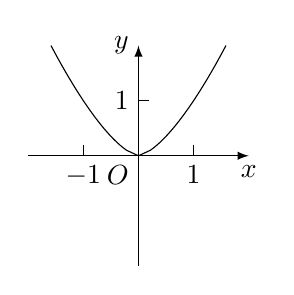
\begin{tikzpicture}[scale = 0.7, >=latex]
\draw [->] (-2,0) -- (2,0) node [below] {$x$};
\draw [->] (0,-2) -- (0,2) node [left] {$y$};
\draw (0,0) node [below left] {$O$};
\draw (1,0.2) -- (1,0) node [below] {$1$};
\draw (0.2,1) -- (0,1) node [left] {$1$};
\draw (-1,0.2) -- (-1,0) node [below] {$-1$};
\draw [domain = 0:4,samples = 400] plot ({\x^(1/3)},{\x^(1/2)});
\draw [domain = 0:4,samples = 400] plot ({-\x^(1/3)},{\x^(1/2)});
\end{tikzpicture}}{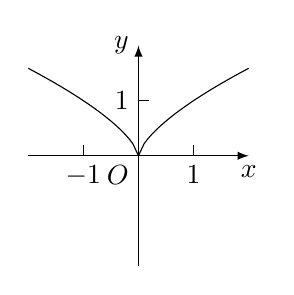
\begin{tikzpicture}[scale = 0.7, >=latex]
\draw [->] (-2,0) -- (2,0) node [below] {$x$};
\draw [->] (0,-2) -- (0,2) node [left] {$y$};
\draw (0,0) node [below left] {$O$};
\draw (1,0.2) -- (1,0) node [below] {$1$};
\draw (0.2,1) -- (0,1) node [left] {$1$};
\draw (-1,0.2) -- (-1,0) node [below] {$-1$};
\draw [domain = 0:4,samples = 400] plot ({\x^(1/2)},{\x^(1/3)});
\draw [domain = 0:4,samples = 400] plot ({-\x^(1/2)},{\x^(1/3)});
\end{tikzpicture}}{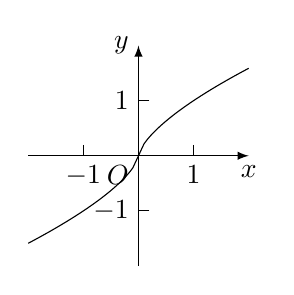
\begin{tikzpicture}[scale = 0.7, >=latex]
\draw [->] (-2,0) -- (2,0) node [below] {$x$};
\draw [->] (0,-2) -- (0,2) node [left] {$y$};
\draw (0,0) node [below left] {$O$};
\draw (1,0.2) -- (1,0) node [below] {$1$};
\draw (0.2,1) -- (0,1) node [left] {$1$};
\draw (-1,0.2) -- (-1,0) node [below] {$-1$};
\draw (0.2,-1) -- (0,-1) node [left] {$-1$};
\draw [domain = 0:4,samples = 400] plot ({\x^(1/2)},{\x^(1/3)});
\draw [domain = 0:4,samples = 400] plot ({-\x^(1/2)},{-\x^(1/3)});
\end{tikzpicture}}


关联目标:

暂未关联目标



标签: 第二单元

答案: 暂无答案

解答或提示: 暂无解答与提示

使用记录:

暂无使用记录


出处: 代数精编第三章函数
\item { (005449)}幂函数$y=x^m$和$y=x^n$在第一象限内的图像$C_1$和$C_2$图像所示, 则$m,n$之间的关系是\bracket{20}.
\begin{center}
    \begin{tikzpicture}[>=latex]
        \draw [->] (-1,0) -- (3,0) node [below] {$x$};
        \draw [->] (0,-1) -- (0,3) node [left] {$y$};
        \draw (0,0) node [below left] {$O$};
        \draw (1,0.2) -- (1,0) node [below] {$1$};
        \draw (0.2,1) -- (0,1) node [left] {$1$};
        \draw [domain = 0.5:2, samples = 400] plot (\x,{\x^(-5/4)});
        \draw [domain = 0.5:2, samples = 400] plot ({\x^(-5/4)},\x);
        \draw (0.5,{0.5^(-5/4)}) node [right] {$C_2$} ({0.5^(-5/4)},0.5) node [above] {$C_1$};
    \end{tikzpicture}
\end{center}
\fourch{$n<m<0$}{$m<n<0$}{$n>m>0$}{$m>n>0$}


关联目标:

暂未关联目标



标签: 第二单元

答案: 暂无答案

解答或提示: 暂无解答与提示

使用记录:

暂无使用记录


出处: 代数精编第三章函数
\item { (005450)}图中, $C_1,C_2,C_3$为幂函数$y=x^a$在第一象限的图像, 则解析式中的指数$\alpha$依次可以取\bracket{20}.
\begin{center}
    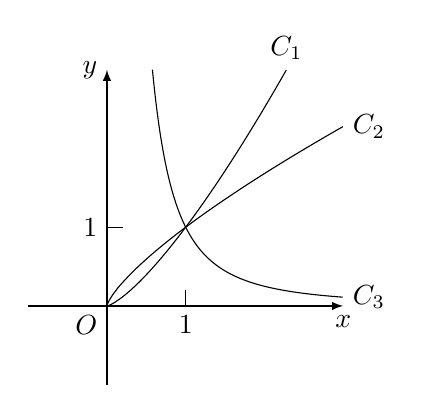
\begin{tikzpicture}[>=latex]
        \draw [->] (-1,0) -- (3,0) node [below] {$x$};
        \draw [->] (0,-1) -- (0,3) node [left] {$y$};
        \draw (0,0) node [below left] {$O$};
        \draw (1,0.2) -- (1,0) node [below] {$1$};
        \draw (0.2,1) -- (0,1) node [left] {$1$};
        \draw [domain = {sqrt(3)/3}:3, samples = 400] plot (\x,{\x^(-2)});
        \draw [domain = 0:3, samples = 400] plot (\x,{\x^(3/4)});
        \draw [domain = 0:{3^(3/4)}, samples = 400] plot (\x,{\x^(4/3)});
        \draw (3,{1/9}) node [right] {$C_3$} (3,{3^(3/4)}) node [right] {$C_2$} ({3^(3/4)},3) node [above] {$C_1$};
    \end{tikzpicture}
\end{center}
\fourch{$\dfrac 43,-2,\dfrac 34$}{$-2,\dfrac 34,\dfrac 43$}{$-2,\dfrac 43,\dfrac 34$}{$\dfrac 34,\dfrac 43,-2$}


关联目标:

暂未关联目标



标签: 第二单元

答案: 暂无答案

解答或提示: 暂无解答与提示

使用记录:

暂无使用记录


出处: 代数精编第三章函数
\item { (005451)}函数$y=x^{\frac 56}$的定义域为\blank{50}, 值域为\blank{50}.


关联目标:

暂未关联目标



标签: 第二单元

答案: 暂无答案

解答或提示: 暂无解答与提示

使用记录:

暂无使用记录


出处: 代数精编第三章函数
\item { (005452)}函数$y=x^{\frac 35}$的定义域为\blank{50}, 值域为\blank{50}.


关联目标:

暂未关联目标



标签: 第二单元

答案: 暂无答案

解答或提示: 暂无解答与提示

使用记录:

暂无使用记录


出处: 代数精编第三章函数
\item { (005453)}函数$y=x^{\frac 85}$的定义域为\blank{50}, 值域为\blank{50}.


关联目标:

暂未关联目标



标签: 第二单元

答案: 暂无答案

解答或提示: 暂无解答与提示

使用记录:

暂无使用记录


出处: 代数精编第三章函数
\item { (005454)}函数$y=x^{-\frac 54}$的定义域为\blank{50}, 值域为\blank{50}.


关联目标:

暂未关联目标



标签: 第二单元

答案: 暂无答案

解答或提示: 暂无解答与提示

使用记录:

暂无使用记录


出处: 代数精编第三章函数
\item { (005455)}函数$y=x^{-\frac 53}$的定义域为\blank{50}, 值域为\blank{50}.


关联目标:

暂未关联目标



标签: 第二单元

答案: 暂无答案

解答或提示: 暂无解答与提示

使用记录:

暂无使用记录


出处: 代数精编第三章函数
\item { (005456)}函数$y=x^{-\frac 23}$的定义域为\blank{50}, 值域为\blank{50}.


关联目标:

暂未关联目标



标签: 第二单元

答案: 暂无答案

解答或提示: 暂无解答与提示

使用记录:

暂无使用记录


出处: 代数精编第三章函数
\item { (005457)}函数$y=-2(x+5)^{-\frac 14}$的定义域为\blank{50}, 值域为\blank{50}.


关联目标:

暂未关联目标



标签: 第二单元

答案: 暂无答案

解答或提示: 暂无解答与提示

使用记录:

暂无使用记录


出处: 代数精编第三章函数
\item { (005458)}函数$y=5(2x-1)^{\frac 34}$的定义域为\blank{50}, 值域为\blank{50}.


关联目标:

暂未关联目标



标签: 第二单元

答案: 暂无答案

解答或提示: 暂无解答与提示

使用记录:

暂无使用记录


出处: 代数精编第三章函数
\item { (005459)}将下列函数图像的标号, 填在相应函数后面的横线上:\\
(1) $y=x^{\frac 23}$:\blank{50}; (2) $y=x^{-2}$:\blank{50}; (3) $y=x^{\frac 12}$:\blank{50};\\
(4) $y=x^{-1}$:\blank{50}; (5) $y=x^{\frac 13}$:\blank{50}; (6)$y=x^{\frac 32}$:\blank{50};\\ (7)$y=x^{\frac 43}$:\blank{50}; (8)$y=x^{-\frac 12}$:\blank{50}; (9)$y=x^{\frac 53}$:\blank{50}.
\begin{center}
    \begin{tikzpicture}[>=latex,scale = 0.6]
        \draw [->] (-2.5,0) -- (2.5,0) node [below] {$x$};
        \draw [->] (0,-2.5) -- (0,2.5) node [left] {$y$};
        \draw (0,0) node [below left] {$O$};
        \draw (0.2,1) -- (0,1) node [left] {$1$} (0.2,-1) -- (0,-1) node [left] {$-1$};
        \draw (1,0.2) -- (1,0) node [below] {$1$} (-1,0.2) -- (-1,0) node [below] {$1$};
        \draw (0,-2.5) node [below] {(A)};
        \draw [domain = 0:2.4, samples = 400] plot (\x,{\x^(1/2)});
    \end{tikzpicture}
    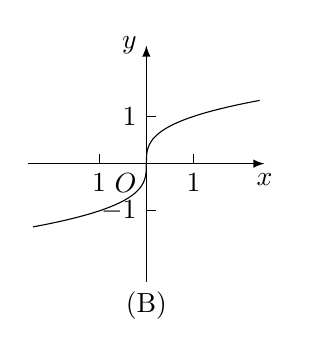
\begin{tikzpicture}[>=latex,scale = 0.6]
        \draw [->] (-2.5,0) -- (2.5,0) node [below] {$x$};
        \draw [->] (0,-2.5) -- (0,2.5) node [left] {$y$};
        \draw (0,0) node [below left] {$O$};
        \draw (0,-2.5) node [below] {(B)};
        \draw (0.2,1) -- (0,1) node [left] {$1$} (0.2,-1) -- (0,-1) node [left] {$-1$};
        \draw (1,0.2) -- (1,0) node [below] {$1$} (-1,0.2) -- (-1,0) node [below] {$1$};
        \draw [domain = 0:2.4, samples = 400] plot (\x,{\x^(1/3)});
        \draw [domain = 0:2.4, samples = 400] plot (-\x,{-\x^(1/3)});
    \end{tikzpicture}
    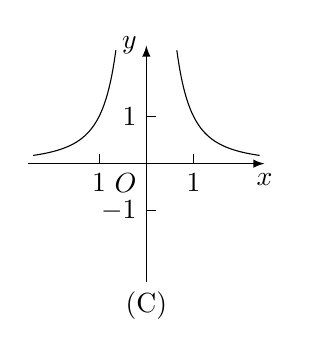
\begin{tikzpicture}[>=latex,scale = 0.6]
        \draw [->] (-2.5,0) -- (2.5,0) node [below] {$x$};
        \draw [->] (0,-2.5) -- (0,2.5) node [left] {$y$};
        \draw (0,0) node [below left] {$O$};
        \draw (0,-2.5) node [below] {(C)};
        \draw (0.2,1) -- (0,1) node [left] {$1$} (0.2,-1) -- (0,-1) node [left] {$-1$};
        \draw (1,0.2) -- (1,0) node [below] {$1$} (-1,0.2) -- (-1,0) node [below] {$1$};
        \draw [domain = {1/sqrt(2.4)}:2.4, samples = 400] plot (\x,{\x^(-2)});
        \draw [domain = {1/sqrt(2.4)}:2.4, samples = 400] plot (-\x,{\x^(-2)});
    \end{tikzpicture}\\
    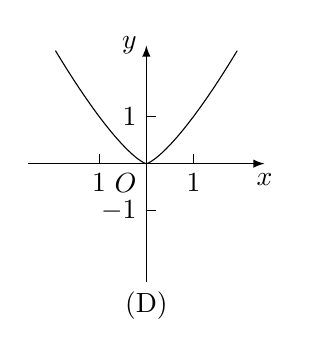
\begin{tikzpicture}[>=latex,scale = 0.6]
        \draw [->] (-2.5,0) -- (2.5,0) node [below] {$x$};
        \draw [->] (0,-2.5) -- (0,2.5) node [left] {$y$};
        \draw (0,0) node [below left] {$O$};
        \draw (0,-2.5) node [below] {(D)};
        \draw (0.2,1) -- (0,1) node [left] {$1$} (0.2,-1) -- (0,-1) node [left] {$-1$};
        \draw (1,0.2) -- (1,0) node [below] {$1$} (-1,0.2) -- (-1,0) node [below] {$1$};
        \draw [domain = 0:{2.4^(3/4)}, samples = 400] plot (\x,{\x^(4/3)});
        \draw [domain = 0:{2.4^(3/4)}, samples = 400] plot (-\x,{\x^(4/3)});
    \end{tikzpicture}
    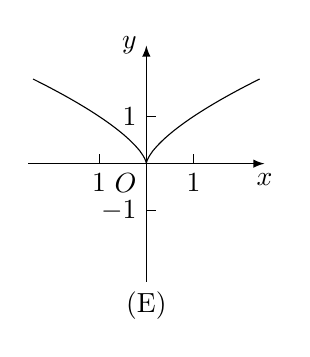
\begin{tikzpicture}[>=latex,scale = 0.6]
        \draw [->] (-2.5,0) -- (2.5,0) node [below] {$x$};
        \draw [->] (0,-2.5) -- (0,2.5) node [left] {$y$};
        \draw (0,0) node [below left] {$O$};
        \draw (0,-2.5) node [below] {(E)};
        \draw (0.2,1) -- (0,1) node [left] {$1$} (0.2,-1) -- (0,-1) node [left] {$-1$};
        \draw (1,0.2) -- (1,0) node [below] {$1$} (-1,0.2) -- (-1,0) node [below] {$1$};
        \draw [domain = 0:2.4, samples = 400] plot (\x,{\x^(2/3)});
        \draw [domain = 0:2.4, samples = 400] plot (-\x,{\x^(2/3)});
    \end{tikzpicture}
    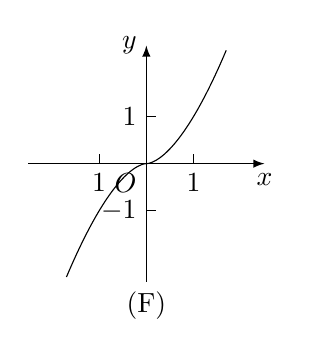
\begin{tikzpicture}[>=latex,scale = 0.6]
        \draw [->] (-2.5,0) -- (2.5,0) node [below] {$x$};
        \draw [->] (0,-2.5) -- (0,2.5) node [left] {$y$};
        \draw (0,0) node [below left] {$O$};
        \draw (0,-2.5) node [below] {(F)};
        \draw (0.2,1) -- (0,1) node [left] {$1$} (0.2,-1) -- (0,-1) node [left] {$-1$};
        \draw (1,0.2) -- (1,0) node [below] {$1$} (-1,0.2) -- (-1,0) node [below] {$1$};
        \draw [domain = 0:{2.4^(3/5)}, samples = 400] plot (\x,{\x^(5/3)});
        \draw [domain = 0:{2.4^(3/5)}, samples = 400] plot (-\x,{-\x^(5/3)});
    \end{tikzpicture}\\
    \begin{tikzpicture}[>=latex,scale = 0.6]
        \draw [->] (-2.5,0) -- (2.5,0) node [below] {$x$};
        \draw [->] (0,-2.5) -- (0,2.5) node [left] {$y$};
        \draw (0,0) node [below left] {$O$};
        \draw (0,-2.5) node [below] {(G)};
        \draw (0.2,1) -- (0,1) node [left] {$1$} (0.2,-1) -- (0,-1) node [left] {$-1$};
        \draw (1,0.2) -- (1,0) node [below] {$1$} (-1,0.2) -- (-1,0) node [below] {$1$};
        \draw [domain = {1/2.4}:2.4] plot (\x,{1/\x});
        \draw [domain = {1/2.4}:2.4] plot (-\x,{-1/\x});
    \end{tikzpicture}
    \begin{tikzpicture}[>=latex,scale = 0.6]
        \draw [->] (-2.5,0) -- (2.5,0) node [below] {$x$};
        \draw [->] (0,-2.5) -- (0,2.5) node [left] {$y$};
        \draw (0,0) node [below left] {$O$};
        \draw (0,-2.5) node [below] {(H)};
        \draw (0.2,1) -- (0,1) node [left] {$1$} (0.2,-1) -- (0,-1) node [left] {$-1$};
        \draw (1,0.2) -- (1,0) node [below] {$1$} (-1,0.2) -- (-1,0) node [below] {$1$};
        \draw [domain = {1/2.4^2}:2.4] plot (\x,{1/\x^(1/2)});
    \end{tikzpicture}
    \begin{tikzpicture}[>=latex,scale = 0.6]
        \draw [->] (-2.5,0) -- (2.5,0) node [below] {$x$};
        \draw [->] (0,-2.5) -- (0,2.5) node [left] {$y$};
        \draw (0,0) node [below left] {$O$};
        \draw (0,-2.5) node [below] {(I)};
        \draw (0.2,1) -- (0,1) node [left] {$1$} (0.2,-1) -- (0,-1) node [left] {$-1$};
        \draw (1,0.2) -- (1,0) node [below] {$1$} (-1,0.2) -- (-1,0) node [below] {$1$};
        \draw [domain = 0:{2.4^(2/3)}] plot (\x,{\x^(3/2)});
    \end{tikzpicture}
\end{center}


关联目标:

暂未关联目标



标签: 第二单元

答案: 暂无答案

解答或提示: 暂无解答与提示

使用记录:

暂无使用记录


出处: 代数精编第三章函数
\item { (005460)}若幂函数$y=x^n$的图像在$0<x<1$时位于直线$y=x$的下方, 则$n$的取值范围是\blank{50}.


关联目标:

暂未关联目标



标签: 第二单元

答案: 暂无答案

解答或提示: 暂无解答与提示

使用记录:

暂无使用记录


出处: 代数精编第三章函数
\item { (005461)}若幂函数$y=x^n$的图像在$0<x<1$时位于直线$y=x$的上方, 则$n$的取值范围是\blank{50}.


关联目标:

暂未关联目标



标签: 第二单元

答案: 暂无答案

解答或提示: 暂无解答与提示

使用记录:

暂无使用记录


出处: 代数精编第三章函数
\item { (005462)}函数$f(x)=x^{k^2-2k-3}$($k\in \mathbf{Z}$)的图像如图所示, 则$k=$\blank{50}.
\begin{center}
    \begin{tikzpicture}[>=latex]
        \draw [->] (-2.5,0) -- (2.5,0) node [below] {$x$};
        \draw [->] (0,-0.5) -- (0,2.5) node [left] {$y$};
        \draw (0,0) node [below left] {$O$};
        \draw (0,-0.5) node [below] {(C)};
        \draw (0.2,1) -- (0,1) node [left] {$1$};
        \draw (1,0.2) -- (1,0) node [below] {$1$} (-1,0.2) -- (-1,0) node [below] {$1$};
        \draw [domain = {1/2.4^(1/4)}:2.4, samples = 400] plot (\x,{\x^(-4)});
        \draw [domain = {1/2.4^(1/4)}:2.4, samples = 400] plot (-\x,{\x^(-4)});
    \end{tikzpicture}
\end{center}


关联目标:

暂未关联目标



标签: 第二单元

答案: 暂无答案

解答或提示: 暂无解答与提示

使用记录:

暂无使用记录


出处: 代数精编第三章函数
\item { (005465)}若实数$a$满足$(\dfrac 34)^{-a}>(\dfrac 43)^{-a}$, 求$a$的取值范围.


关联目标:

暂未关联目标



标签: 第二单元

答案: 暂无答案

解答或提示: 暂无解答与提示

使用记录:

暂无使用记录


出处: 代数精编第三章函数
\item { (005466)}若实数$a$满足$a^{-2}>3^{-2}$, 求$a$的取值范围.


关联目标:

暂未关联目标



标签: 第二单元

答案: 暂无答案

解答或提示: 暂无解答与提示

使用记录:

暂无使用记录


出处: 代数精编第三章函数
\item { (005467)}若实数$a$满足$0.01^{-3}>a^{-3}$, 求$a$的取值范围.


关联目标:

暂未关联目标



标签: 第二单元

答案: 暂无答案

解答或提示: 暂无解答与提示

使用记录:

暂无使用记录


出处: 代数精编第三章函数
\item { (005468)}将$2.5^{\frac 23}$, $(-1.4)^{\frac 23}$, $(-3)^{\frac 13}$从小到大排列:\blank{50}.


关联目标:

暂未关联目标



标签: 第二单元

答案: 暂无答案

解答或提示: 暂无解答与提示

使用记录:

暂无使用记录


出处: 代数精编第三章函数
\item { (005469)}将$4.1^{\frac 25}$, $3.8^{-\frac 23}$, $(-1.9)^{\frac 35}$从小到大排列:\blank{50}.


关联目标:

暂未关联目标



标签: 第二单元

答案: 暂无答案

解答或提示: 暂无解答与提示

使用记录:

暂无使用记录


出处: 代数精编第三章函数
\item { (005470)}将$0.16^{-\frac 34}$, $0.5^{-\frac 32}$, $6.25^{\frac 38}$从小到大排列:\blank{50}.


关联目标:

暂未关联目标



标签: 第二单元

答案: 暂无答案

解答或提示: 暂无解答与提示

使用记录:

暂无使用记录


出处: 代数精编第三章函数
\item { (005471)}已知函数$y=x^{n^2-2n-3}$($n\in \mathbf{Z}$)的图像与两坐标轴都无公共点, 且其图像关于$y$轴对称, 求$n$的值, 并画出相应的函数图像.


关联目标:

暂未关联目标



标签: 第二单元

答案: 暂无答案

解答或提示: 暂无解答与提示

使用记录:

暂无使用记录


出处: 代数精编第三章函数
\item { (005472)}函数$y=\sqrt {x^2+2x-3}$为减函数的区间是\bracket{20}.
\fourch{$(-\infty ,-3]$}{$[-1,+\infty)$}{$(-\infty ,-1]$}{$[1,+\infty)$}


关联目标:

暂未关联目标



标签: 第二单元

答案: 暂无答案

解答或提示: 暂无解答与提示

使用记录:

暂无使用记录


出处: 代数精编第三章函数
\item { (005473)}若函数$y=(2k+1)x+b$在$(-\infty,+\infty)$上是减函数, 则\bracket{20}.
\fourch{$k>\dfrac 12$}{$k<\dfrac 12$}{$k>-\dfrac 12$}{$k<-\dfrac 12$}


关联目标:

暂未关联目标



标签: 第二单元

答案: 暂无答案

解答或提示: 暂无解答与提示

使用记录:

暂无使用记录


出处: 代数精编第三章函数
\item { (005474)}若函数$f(x)=4x^2-mx+5$在区间$[-2,+\infty)$上是增函数, 在区间$(-\infty ,-2]$上是减函数, 则$f(1)$等于\bracket{20}.
\fourch{$-7$}{$1$}{$17$}{$25$}


关联目标:

暂未关联目标



标签: 第二单元

答案: 暂无答案

解答或提示: 暂无解答与提示

使用记录:

暂无使用记录


出处: 代数精编第三章函数
\item { (005475)}若函数$y=x^2+2(a-2)x+5$在区间$(4,+\infty)$上是增函数, 则实数$a$的取值范围是\bracket{20}.
\fourch{$a\le -2$}{$a\ge -2$}{$a\le -6$}{$a\ge -6$}


关联目标:

暂未关联目标



标签: 第二单元

答案: 暂无答案

解答或提示: 暂无解答与提示

使用记录:

暂无使用记录


出处: 代数精编第三章函数
\item { (005476)}下列函数中, 在区间$(0,2)$上为增函数的是\bracket{20}.
\fourch{$y=-3x+1$}{$y=\sqrt[3]x$}{$y=x^2-4x+3$}{$y=\dfrac 4x$}


关联目标:

暂未关联目标



标签: 第二单元

答案: 暂无答案

解答或提示: 暂无解答与提示

使用记录:

暂无使用记录


出处: 代数精编第三章函数
\item { (005477)}若函数$f(x)$在定义域$\mathbf{R}$上为增函数, 且$f(x)<0$, 则下列函数在$\mathbf{R}$上为增函数的是\bracket{20}.
\fourch{$y=|f(x)|$}{$y=\dfrac 1{f(x)}$}{$y=[ f(x) ]^2$}{$y=[ f(x) ]^3$}


关联目标:

暂未关联目标



标签: 第二单元

答案: 暂无答案

解答或提示: 暂无解答与提示

使用记录:

暂无使用记录


出处: 代数精编第三章函数
\item { (005478)}函数$y=\dfrac 1{\sqrt {x^2-4x+5}}$为增函数的区间是\blank{50}, 为减函数的区间是\blank{50}.


关联目标:

暂未关联目标



标签: 第二单元

答案: 暂无答案

解答或提示: 暂无解答与提示

使用记录:

暂无使用记录


出处: 代数精编第三章函数
\item { (005479)}函数$y=\dfrac 1{\sqrt {3+2x-x^2}}$为增函数的区间是\blank{50}.


关联目标:

暂未关联目标



标签: 第二单元

答案: 暂无答案

解答或提示: 暂无解答与提示

使用记录:

暂无使用记录


出处: 代数精编第三章函数
\item { (005480)}函数$y=|3x-5|$为减函数的区间是\blank{50}.


关联目标:

暂未关联目标



标签: 第二单元

答案: 暂无答案

解答或提示: 暂无解答与提示

使用记录:

暂无使用记录


出处: 代数精编第三章函数
\item { (005481)}函数$y=|x^2-2x-3|$为增函数的区间是\blank{50}.


关联目标:

暂未关联目标



标签: 第二单元

答案: 暂无答案

解答或提示: 暂无解答与提示

使用记录:

暂无使用记录


出处: 代数精编第三章函数
\item { (005482)}函数$y=\dfrac{1-x}{1+x}$为减函数的区间是\blank{50}.


关联目标:

暂未关联目标



标签: 第二单元

答案: 暂无答案

解答或提示: 暂无解答与提示

使用记录:

暂无使用记录


出处: 代数精编第三章函数
\item { (005483)}定义在$[1, 3]$上的函数$f(x)$为减函数, 求满足不等式$f(1-a)-f(3-a^2)>0$的解集.


关联目标:

暂未关联目标



标签: 第二单元

答案: 暂无答案

解答或提示: 暂无解答与提示

使用记录:

暂无使用记录


出处: 代数精编第三章函数
\item { (005484)}已知$f(x)=-x^3-x+1$($x\in \mathbf{R}$), 求证$y=f(x)$在定义域上为减函数.


关联目标:

暂未关联目标



标签: 第二单元

答案: 暂无答案

解答或提示: 暂无解答与提示

使用记录:

暂无使用记录


出处: 代数精编第三章函数
\item { (005485)}求证: 函数$f(x)=x+\dfrac 1x$在$(0, 1)$上是减函数, 在$(1,+\infty)$上是增函数.


关联目标:

暂未关联目标



标签: 第二单元

答案: 暂无答案

解答或提示: 暂无解答与提示

使用记录:

暂无使用记录


出处: 代数精编第三章函数
\item { (005486)}求证: $f(x)=\sqrt x-\dfrac 1x$在定义域上是增函数.


关联目标:

暂未关联目标



标签: 第二单元

答案: 暂无答案

解答或提示: 暂无解答与提示

使用记录:

暂无使用记录


出处: 代数精编第三章函数
\item { (005487)}已知常数$m,n$满足$mn<2$, 求证: 函数$f(x)=\dfrac{mx+1}{2x+n}$在$(-\dfrac n2,+\infty)$上为减函数.


关联目标:

暂未关联目标



标签: 第二单元

答案: 暂无答案

解答或提示: 暂无解答与提示

使用记录:

暂无使用记录


出处: 代数精编第三章函数
\item { (005488)}已知$f(x)=x^2+1$, $g(x)=x^4+2x^2+2$, 是否存在实数$\lambda$, 使得$F(x)=g(x)-\lambda f(x)$在$(-\infty ,-1)$上是减函数, 在$(-1,0)$上是增函数? 说明理由.


关联目标:

暂未关联目标



标签: 第二单元

答案: 暂无答案

解答或提示: 暂无解答与提示

使用记录:

暂无使用记录


出处: 代数精编第三章函数
\item { (005489)}已知函数$f(x)$在区间$(-\infty ,+\infty)$上是增函数, 又实数$a,b$满足$a+b\ge 0$, 求证: $f(a)+f(b)\ge f(-a)+f(-b)$.


关联目标:

暂未关联目标



标签: 第二单元

答案: 暂无答案

解答或提示: 暂无解答与提示

使用记录:

暂无使用记录


出处: 代数精编第三章函数
\item { (005490)}$f(x)$是定义在$\mathbf{R}^+$的增函数, 且$f(\dfrac xy)=f(x)-f(y)$.\\
(1) 求$f(1)$的值;\\
(2) 若$f(6)=1$, 解不等式$f(x+3)-f(\dfrac 1x)<2$.


关联目标:

暂未关联目标



标签: 第二单元

答案: 暂无答案

解答或提示: 暂无解答与提示

使用记录:

暂无使用记录


出处: 代数精编第三章函数
\item { (005491)}若$f(x)=(m-1)x^2+3mx+3$为偶函数, 则$f(x)$在区间$(-4,2)$上\bracket{20}.
\twoch{是增函数}{是减函数}{先是增函数后是减函数}{先是减函数后是增函数}


关联目标:

暂未关联目标



标签: 第二单元

答案: 暂无答案

解答或提示: 暂无解答与提示

使用记录:

暂无使用记录


出处: 代数精编第三章函数
\item { (005492)}函数$f(x)=\begin{cases}   1-x, & x>0,  \\ 0, & x=0,  \\1+x, & x<0,  \end{cases}$则该函数\bracket{20}.
\twoch{是奇函数, 但不是偶函数}{是偶函数, 但不是奇函数}{既是奇函数, 也是偶函数}{既不是奇函数, 也不是偶函数}


关联目标:

暂未关联目标



标签: 第二单元

答案: 暂无答案

解答或提示: 暂无解答与提示

使用记录:

暂无使用记录


出处: 代数精编第三章函数
\item { (005493)}下列函数中既是奇函数, 又在定义域上为增函数的是\bracket{20}.
\fourch{$f(x)=3x+1$}{$f(x)=\dfrac 1x$}{$f(x)=1-\dfrac 1x$}{$f(x)=x^3$}


关联目标:

暂未关联目标



标签: 第二单元

答案: 暂无答案

解答或提示: 暂无解答与提示

使用记录:

暂无使用记录


出处: 代数精编第三章函数
\item { (005494)}若$f(x)$为定义在区间$[-6, 6]$上的偶函数, 且满足$f(3)>f(1)$, 则恒成立的是\bracket{20}.
\fourch{$f(-1)<f(3)$}{$f(0)<f(6)$}{$f(3)>f(2)$}{$f(2)>f(0)$}


关联目标:

暂未关联目标



标签: 第二单元

答案: 暂无答案

解答或提示: 暂无解答与提示

使用记录:

暂无使用记录


出处: 代数精编第三章函数
\item { (005495)}函数$f(x)=\dfrac{\sqrt {1-x^2}}{2-|x+2|}$\bracket{20}.
\twoch{是奇函数, 但不是偶函数}{是偶函数, 但不是奇函数}{既是奇函数, 又是偶函数}{既不是奇函数, 也不是偶函数}


关联目标:

暂未关联目标



标签: 第二单元

答案: 暂无答案

解答或提示: 暂无解答与提示

使用记录:

暂无使用记录


出处: 代数精编第三章函数
\item { (005496)}已知$f(x)$是奇函数, 则下列各点中在函数$y=f(x)$的图像上的点的是\bracket{20}.
\fourch{$(a,f(-a))$}{$(-a,-f(a))$}{$(\dfrac 1a,-f(\dfrac 1a))$}{$(-\sin a,-f(-\sin a))$}


关联目标:

暂未关联目标



标签: 第二单元

答案: 暂无答案

解答或提示: 暂无解答与提示

使用记录:

暂无使用记录


出处: 代数精编第三章函数
\item { (005497)}若$f(x)$是定义在$\mathbf{R}$上的偶函数, 且当$x<0$时, $f(x)=2x-3$, 则当$x>0$时, $f(x)=$\blank{50}.


关联目标:

暂未关联目标



标签: 第二单元

答案: 暂无答案

解答或提示: 暂无解答与提示

使用记录:

暂无使用记录


出处: 代数精编第三章函数
\item { (005498)}若奇函数$f(x)$的定义域是$\mathbf{R}$, 则$f(0)=$\blank{50}.


关联目标:

暂未关联目标



标签: 第二单元

答案: 暂无答案

解答或提示: 暂无解答与提示

使用记录:

暂无使用记录


出处: 代数精编第三章函数
\item { (005499)}若奇函数$f(x)$在区间$[-3, -1]$上是增函数, 且有最大值$-2$, 则$f(x)$在$[1, 3]$上是\blank{50}函数(填``增''或``减''), 且最小值等于\blank{50}.


关联目标:

暂未关联目标



标签: 第二单元

答案: 暂无答案

解答或提示: 暂无解答与提示

使用记录:

暂无使用记录


出处: 代数精编第三章函数
\item { (005500)}设$f(x)$为定义在$\mathbf{R}$上的偶函数, 且$f(x)$在$[0,+\infty)$上是增函数, 则$f(-4)$, $f(-2)$, $f(3)$由小到大的排列顺序为\blank{50}.


关联目标:

暂未关联目标



标签: 第二单元

答案: 暂无答案

解答或提示: 暂无解答与提示

使用记录:

暂无使用记录


出处: 代数精编第三章函数
\item { (005501)}若函数$f(x)=x^5+px^3+qx-8$满足$f(-2)=10$, 则$f(2)=$\bracket{20}.
\fourch{$10$}{$-10$}{$-26$}{$-18$}


关联目标:

暂未关联目标



标签: 第二单元

答案: 暂无答案

解答或提示: 暂无解答与提示

使用记录:

暂无使用记录


出处: 代数精编第三章函数
\item { (005502)}设$f(x)$在$R$上是奇函数, 且当$x\in [0,+\infty)$时, $f(x)=x(1+\sqrt[3]x)$, 那么当$x\in (-\infty ,0)$时, $f(x)=$\bracket{20}.
\fourch{$-x(1+\sqrt[3]x)$}{$x(1+\sqrt[3]x)$}{$-x(1-\sqrt[3]x)$}{$x(1-\sqrt[3]x)$}


关联目标:

暂未关联目标



标签: 第二单元

答案: 暂无答案

解答或提示: 暂无解答与提示

使用记录:

暂无使用记录


出处: 代数精编第三章函数
\item { (005503)}若函数$f(x)=8+2x-x^2$, 记$g(x)=f(2-x^2)$, 则$g(x)$\bracket{20}.
\fourch{在(-2, 0)上是增函数}{在(0, 2)上是增函数}{在(-1, 0)上是减函数}{在(0, 1)上是减函数}


关联目标:

暂未关联目标



标签: 第二单元

答案: 暂无答案

解答或提示: 暂无解答与提示

使用记录:

暂无使用记录


出处: 代数精编第三章函数
\item { (005504)}函数$f(x)=x|x|-2x$是\bracket{20}.
\twoch{偶函数, 且在(-1, 1)上是增函数}{奇函数, 且在(-1, 1)上是减函数}{偶函数, 且在(-1, 1)上是减函数}{奇函数, 且在(-1, 1)上是增函数}


关联目标:

暂未关联目标



标签: 第二单元

答案: 暂无答案

解答或提示: 暂无解答与提示

使用记录:

暂无使用记录


出处: 代数精编第三章函数
\item { (005505)}若函数$y=f(x)$是偶函数, 其图像与$x$轴有四个交点, 则方程$f(x)=0$的所有实数根之和为\bracket{20}.
\fourch{$4$}{$2$}{$1$}{$0$}


关联目标:

暂未关联目标



标签: 第二单元

答案: 暂无答案

解答或提示: 暂无解答与提示

使用记录:

暂无使用记录


出处: 代数精编第三章函数
\item { (005506)}函数$f(x)=\dfrac x{2^{1+x}+2^{1-x}}$\bracket{20}.
\twoch{是奇函数, 但不是偶函数}{是偶函数, 但不是奇函数}{既是奇函数, 又是偶函数}{既不是奇函数, 也不是偶函数}


关联目标:

暂未关联目标



标签: 第二单元

答案: 暂无答案

解答或提示: 暂无解答与提示

使用记录:

暂无使用记录


出处: 代数精编第三章函数
\item { (005507)}已知奇函数$f(x)$在$x>0$时的表达式为$f(x)=2x-\dfrac 12$, 则当$x\le -\dfrac 14$时, 恒有\bracket{20}.
\fourch{$f(x)>0$}{$f(x)<0$}{$f(x)-f(-x)\le 0$}{$f(x)-f(-x)>0$}


关联目标:

暂未关联目标



标签: 第二单元

答案: 暂无答案

解答或提示: 暂无解答与提示

使用记录:

暂无使用记录


出处: 代数精编第三章函数
\item { (005508)}$f(x)+f(2-x)+2=0$对任何实数$x$都成立, 则$f(x)$的图像\bracket{20}.
\twoch{关于直线$x=1$成轴对称图形}{关于直线$x=2$成轴对称图形}{关于点$(1, -1)$成中心对称图形}{关于点$(-1,1)$成中心对称图形}


关联目标:

暂未关联目标



标签: 第二单元

答案: 暂无答案

解答或提示: 暂无解答与提示

使用记录:

暂无使用记录


出处: 代数精编第三章函数
\item { (005509)}已知$f(x),g(x)$都是定义在$\mathbf{R}$上的函数, $f(x)$为奇函数, $g(x)$为偶函数, 且$f(x)\cdot g(x)$恒不为$0$, 判断下列函数的奇偶性:
(1)$f(x)+g(x)$:\blank{50}; (2)$f(x)\cdot g(x)$:\blank{50}; (3)$f[f(x)]$:\blank{50}; (4)$f[g(x)]$:\blank{50}; (5)$g[f(x)]$:\blank{50}; (6)$g[g(x)]$:\blank{50}.


关联目标:

暂未关联目标



标签: 第二单元

答案: 暂无答案

解答或提示: 暂无解答与提示

使用记录:

暂无使用记录


出处: 代数精编第三章函数
\item { (005510)}判断函数$f(x)=5$的奇偶性:\blank{50}.


关联目标:

暂未关联目标



标签: 第二单元

答案: 暂无答案

解答或提示: 暂无解答与提示

使用记录:

暂无使用记录


出处: 代数精编第三章函数
\item { (005511)}判断函数$f(x)=\sqrt {x^2-1}+\sqrt {1-x^2}$的奇偶性:\blank{50}.


关联目标:

暂未关联目标



标签: 第二单元

答案: 暂无答案

解答或提示: 暂无解答与提示

使用记录:

暂无使用记录


出处: 代数精编第三章函数
\item { (005512)}判断函数$f(x)=x^2-2x^2+3$的奇偶性:\blank{50}.


关联目标:

暂未关联目标



标签: 第二单元

答案: 暂无答案

解答或提示: 暂无解答与提示

使用记录:

暂无使用记录


出处: 代数精编第三章函数
\item { (005513)}判断函数$x\in [-4,4)$的奇偶性:\blank{50}.


关联目标:

暂未关联目标



标签: 第二单元

答案: 暂无答案

解答或提示: 暂无解答与提示

使用记录:

暂无使用记录


出处: 代数精编第三章函数
\item { (005514)}判断函数$f(x)=|3x+2|-|3x-2|$的奇偶性:\blank{50}.


关联目标:

暂未关联目标



标签: 第二单元

答案: 暂无答案

解答或提示: 暂无解答与提示

使用记录:

暂无使用记录


出处: 代数精编第三章函数
\item { (005515)}判断函数$f(x)=\dfrac{x^2(x-1)}{x-1}$的奇偶性:\blank{50}.


关联目标:

暂未关联目标



标签: 第二单元

答案: 暂无答案

解答或提示: 暂无解答与提示

使用记录:

暂无使用记录


出处: 代数精编第三章函数
\item { (005516)}判断函数$f(x)=\dfrac 12[g(x)-g(-x)]$的奇偶性:\blank{50}.


关联目标:

暂未关联目标



标签: 第二单元

答案: 暂无答案

解答或提示: 暂无解答与提示

使用记录:

暂无使用记录


出处: 代数精编第三章函数
\item { (005517)}求证: 函数$f(x)=\dfrac{x+1+\sqrt {1+x^2}}{x-1+\sqrt {1+x^2}}$是奇函数.


关联目标:

暂未关联目标



标签: 第二单元

答案: 暂无答案

解答或提示: 暂无解答与提示

使用记录:

暂无使用记录


出处: 代数精编第三章函数
\item { (005518)}求证: 函数$f(x)=\begin{cases}
   x(1-x), &  x>0,  \\ x(1+x), &  x<0  \end{cases}$是奇函数.


关联目标:

暂未关联目标



标签: 第二单元

答案: 暂无答案

解答或提示: 暂无解答与提示

使用记录:

暂无使用记录


出处: 代数精编第三章函数
\item { (005519)}已知奇函数$f(x)$在定义域$(-l, l)$上是减函数, 求满足$f(1-m)+f(1-m^2)<0$的实数$m$的取值范围.


关联目标:

暂未关联目标



标签: 第二单元

答案: 暂无答案

解答或提示: 暂无解答与提示

使用记录:

暂无使用记录


出处: 代数精编第三章函数
\item { (005520)}已知偶函数$f(x)$在$[0,+\infty)$上是增函数.求不等式$f(2x+5)<f(x^2+2)$的解集.


关联目标:

暂未关联目标



标签: 第二单元

答案: 暂无答案

解答或提示: 暂无解答与提示

使用记录:

暂无使用记录


出处: 代数精编第三章函数
\item { (005521)}是否存在既是奇函数又是偶函数的函数? 说明理由


关联目标:

暂未关联目标



标签: 第二单元

答案: 暂无答案

解答或提示: 暂无解答与提示

使用记录:

暂无使用记录


出处: 代数精编第三章函数
\item { (005522)}求证: 定义域为$(-l,l)$的任何函数都能表示成一个奇函数与一个偶函数之和.


关联目标:

暂未关联目标



标签: 第二单元

答案: 暂无答案

解答或提示: 暂无解答与提示

使用记录:

暂无使用记录


出处: 代数精编第三章函数
\item { (005523)}下列函数中有反函数的是\bracket{20}.
\fourch{$y=3+\sqrt {x^2+5}$}{$y=\dfrac 1{x^2+1}$}{$y=\sqrt [3]{2x-1}+2$}{$y=\begin{cases}
   x^2-3, &  x\ge 0,  \\3x, &  x<0  \end{cases}$}


关联目标:

暂未关联目标



标签: 第二单元

答案: 暂无答案

解答或提示: 暂无解答与提示

使用记录:

暂无使用记录


出处: 代数精编第三章函数
\item { (005524)}函数$y=\sqrt {x^2-2x+3}$($x\le 1$)的反函数的定义域是\bracket{20}.
\fourch{$[0,+\infty)$}{$(2,+\infty)$}{$(-\infty ,1]$}{$[\sqrt 2,+\infty)$}


关联目标:

暂未关联目标



标签: 第二单元

答案: 暂无答案

解答或提示: 暂无解答与提示

使用记录:

暂无使用记录


出处: 代数精编第三章函数
\item { (005525)}设$f(x)=\dfrac{2x+1}{4x+3}$($x\in \mathbf{R}$, 且$x\ne -\dfrac 34$), 则$f^{-1}(2)$的值等于\bracket{20}.
\fourch{$-\dfrac 56$}{$-\dfrac 25$}{$\dfrac 25$}{$\dfrac 5{11}$}


关联目标:

暂未关联目标



标签: 第二单元

答案: 暂无答案

解答或提示: 暂无解答与提示

使用记录:

暂无使用记录


出处: 代数精编第三章函数
\item { (005526)}函数$y=x^2+2x$($x<-1$)的反函数是\bracket{20}.
\twoch{$y=\sqrt {x+1}-1$($x<-1$)}{$y=\sqrt {x+1}-1$($x>-1$)}{$y=-\sqrt {x+1}-1$($x<-1$)}{$y=-\sqrt {x+1}-1$($x>-1$)}


关联目标:

暂未关联目标



标签: 第二单元

答案: 暂无答案

解答或提示: 暂无解答与提示

使用记录:

暂无使用记录


出处: 代数精编第三章函数
\item { (005527)}若函数$y=g(x)$的图像与函数$f(x)=(x-1)^2$($x\le 1$)的图像关于直线$y=x$对称.则$g(x)$的表达式是\bracket{20}.
\twoch{$g(x)=1-\sqrt x$($x\ge 0$)}{$g(x)=1+\sqrt x$($x\ge 0$)}{$g(x)=\sqrt {1-x}$($x\le 1$)}{$g(x)=\sqrt {1+x}$($x\ge -1$)}


关联目标:

暂未关联目标



标签: 第二单元

答案: 暂无答案

解答或提示: 暂无解答与提示

使用记录:

暂无使用记录


出处: 代数精编第三章函数
\item { (005528)}函数$y=\dfrac{ax+b}{cx+1}$($a\ne bc$)的反函数是$y=\dfrac{x+2}{3x+1}$, 则的$a,b,c$值依次为\bracket{20}.
\fourch{$1,-2,-3$}{$-1,2,3$}{$-1, 2, -3$}{$1, 2, 3$}


关联目标:

暂未关联目标



标签: 第二单元

答案: 暂无答案

解答或提示: 暂无解答与提示

使用记录:

暂无使用记录


出处: 代数精编第三章函数
\item { (005529)}若函数$f(x)=\dfrac{x-2}{x+m}$的反函数$f^{-1}(x)=f(x)$, 则$m$的值是\bracket{20}.
\fourch{$1$}{$-1$}{$2$}{$-2$}


关联目标:

暂未关联目标



标签: 第二单元

答案: 暂无答案

解答或提示: 暂无解答与提示

使用记录:

暂无使用记录


出处: 代数精编第三章函数
\item { (005530)}若函数$f(x)$的图像经过点$(0, -1)$, 则函数$f(x+4)$的反函数的图像必经过点\bracket{20}.
\fourch{$(—1,4)$}{$(-4,-1)$}{$(-1,-4)$}{$(1,-4)$}


关联目标:

暂未关联目标



标签: 第二单元

答案: 暂无答案

解答或提示: 暂无解答与提示

使用记录:

暂无使用记录


出处: 代数精编第三章函数
\item { (005531)}已知函数$y=-\sqrt {1-x^2}$的反函数是$y=-\sqrt {1-x^2}$, 则原函数的定义域``最大''可以是\blank{50}.


关联目标:

暂未关联目标



标签: 第二单元

答案: 暂无答案

解答或提示: 暂无解答与提示

使用记录:

暂无使用记录


出处: 代数精编第三章函数
\item { (005532)}已知函数$y=\dfrac 13x+m$与$y=nx-6$互为反函数, 则$m=$\blank{50}, $n=$\blank{50}.


关联目标:

暂未关联目标



标签: 第二单元

答案: 暂无答案

解答或提示: 暂无解答与提示

使用记录:

暂无使用记录


出处: 代数精编第三章函数
\item { (005533)}若点$(1, 2)$既在函数$y=\sqrt {ax+b}$的图像上.又在其反函数的图像上, 则$a=$\blank{50}, $b=$\blank{50}.


关联目标:

暂未关联目标



标签: 第二单元

答案: 暂无答案

解答或提示: 暂无解答与提示

使用记录:

暂无使用记录


出处: 代数精编第三章函数
\item { (005534)}若$y=\dfrac{1+x}{1-x}$($x\ne 1$), 则其反函数$f^{-1}(x)=$\blank{50}.


关联目标:

暂未关联目标



标签: 第二单元

答案: 暂无答案

解答或提示: 暂无解答与提示

使用记录:

暂无使用记录


出处: 代数精编第三章函数
\item { (005535)}若$f(x)=x^{\frac 23}$($x\le 0$), 则其反函数$f^{-1}(x)=$\blank{50}.


关联目标:

暂未关联目标



标签: 第二单元

答案: 暂无答案

解答或提示: 暂无解答与提示

使用记录:

暂无使用记录


出处: 代数精编第三章函数
\item { (005536)}若$f(x)=-\sqrt {1-x^2}$($0\le x\le 1$), 则其反函数$f^{-1}(x)=$\blank{50}.


关联目标:

暂未关联目标



标签: 第二单元

答案: 暂无答案

解答或提示: 暂无解答与提示

使用记录:

暂无使用记录


出处: 代数精编第三章函数
\item { (005537)}若$f(x)=\sqrt {x^2-4}$($x\le -2$), 则其反函数$f^{-1}(x)=$\blank{50}.


关联目标:

暂未关联目标



标签: 第二单元

答案: 暂无答案

解答或提示: 暂无解答与提示

使用记录:

暂无使用记录


出处: 代数精编第三章函数
\item { (005538)}若$f(x)=\begin{cases}
   x^2, & x\le 0,  \\ -3x, & x>0,  \end{cases}$ 则其反函数$f^{-1}(x)=$\blank{50}.


关联目标:

暂未关联目标



标签: 第二单元

答案: 暂无答案

解答或提示: 暂无解答与提示

使用记录:

暂无使用记录


出处: 代数精编第三章函数
\item { (005539)}若$f(x)=\begin{cases}
   x, & 0\le x\le 1,  \\1-x, & -1\le x<0,  \end{cases}$ 则其反函数$f^{-1}(x)=$\blank{50}.


关联目标:

暂未关联目标



标签: 第二单元

答案: 暂无答案

解答或提示: 暂无解答与提示

使用记录:

暂无使用记录


出处: 代数精编第三章函数
\item { (005540)}若$f(x)=\begin{cases}
   x^2-1,  & x\ge 0,  \\2x-1, & x<0,  \end{cases}$ 则其反函数$f^{-1}(x)=$\blank{50}.


关联目标:

暂未关联目标



标签: 第二单元

答案: 暂无答案

解答或提示: 暂无解答与提示

使用记录:

暂无使用记录


出处: 代数精编第三章函数
\item { (005541)}已知函数$f(x)=\dfrac{x+1}{x-1}$, $g(x)=f^{-1}(-x)$, 则$g(x)$\bracket{20}.
\twoch{在$(-\infty ,+\infty)$上是增函数}{在$(-\infty ,-1)$上是增函数}{在$(1,+\infty)$上是减函数}{在$(-\infty ,-1)$上是减函数}


关联目标:

暂未关联目标



标签: 第二单元

答案: 暂无答案

解答或提示: 暂无解答与提示

使用记录:

暂无使用记录


出处: 代数精编第三章函数
\item { (005542)}若函数$y=\sqrt {x-m}$与其反函数的图像有公共点, 则$m$的取值范围是\bracket{20}.
\fourch{$m\ge \dfrac 14$}{$m\le \dfrac 14$}{$m\ge 0$}{$m\le 0$}


关联目标:

暂未关联目标



标签: 第二单元

答案: 暂无答案

解答或提示: 暂无解答与提示

使用记录:

暂无使用记录


出处: 代数精编第三章函数
\item { (005543)}已知$y=g(x)$是函数$y=f(x)$的反函数, 又$y=h(x)$与$y=g(x)$的图像关于原点$O(0,0)$对称, 则$h(x)$的表达式是\bracket{20}.
\fourch{$y=f^{-1}(x)$}{$y=-f^{-1}(x)$}{$y=f^{-1}(-x)$}{$y=-f^{-1}(-x)$}


关联目标:

暂未关联目标



标签: 第二单元

答案: 暂无答案

解答或提示: 暂无解答与提示

使用记录:

暂无使用记录


出处: 代数精编第三章函数
\item { (005544)}若幂函数$f(x)$是奇函数, 则$f^{-1}(1)=$\blank{50}, $f^{-1}(-1)=$\blank{50}.


关联目标:

暂未关联目标



标签: 第二单元

答案: 暂无答案

解答或提示: 暂无解答与提示

使用记录:

暂无使用记录


出处: 代数精编第三章函数
\item { (005545)}若$f(x)=\dfrac{2x-1}{x+a}$存在反函数, 则实数$a$的取值范围是\blank{50}.


关联目标:

暂未关联目标



标签: 第二单元

答案: 暂无答案

解答或提示: 暂无解答与提示

使用记录:

暂无使用记录


出处: 代数精编第三章函数
\item { (005546)}若$f(x)=2x^2-4x+9$($x\ge 1$), 且满足$f^{-1}(a+1)=3$, 则$f(a)=$\blank{50}.


关联目标:

暂未关联目标



标签: 第二单元

答案: 暂无答案

解答或提示: 暂无解答与提示

使用记录:

暂无使用记录


出处: 代数精编第三章函数
\item { (005547)}已知定义域为$(-\infty ,0]$的函数$f(x)$满足$f(x-1)=x^2-2x$, 则$f^{-1}(-\dfrac 12)=$\blank{50}.


关联目标:

暂未关联目标



标签: 第二单元

答案: 暂无答案

解答或提示: 暂无解答与提示

使用记录:

暂无使用记录


出处: 代数精编第三章函数
\item { (005548)}求函数$f(x)=\begin{cases}
   x+1, &  x>0,  \\ x-1, &  x<0  \end{cases}$的反函数, 并作出其反函数的图像.


关联目标:

暂未关联目标



标签: 第二单元

答案: 暂无答案

解答或提示: 暂无解答与提示

使用记录:

暂无使用记录


出处: 代数精编第三章函数
\item { (005549)}已知函数$f(x)=x^2+2x+1$.\\
(1) 若函数的定义域是$(-\infty ,+\infty)$, 这个函数有没有反函数?\\
(2) 若函数的定义域是$[0,+\infty)$, 求其反函数;\\
(3) 若函数的定义域是$(-\infty ,-1]$, 求其反函数.


关联目标:

暂未关联目标



标签: 第二单元

答案: 暂无答案

解答或提示: 暂无解答与提示

使用记录:

暂无使用记录


出处: 代数精编第三章函数
\item { (005550)}若关于$x$的方程$x^2+2(m+3)x+2m+14=0$有两个实数根, 且一个比$4$大, 另一个比$4$小, 求实数$m$的取值范围.


关联目标:

暂未关联目标



标签: 第二单元

答案: 暂无答案

解答或提示: 暂无解答与提示

使用记录:

暂无使用记录


出处: 代数精编第三章函数
\item { (005551)}若关于$x$的方程$x^2+2mx-(m-12)=0$的两根都大于$2$, 求实数$m$的取值范围.


关联目标:

暂未关联目标



标签: 第二单元

答案: 暂无答案

解答或提示: 暂无解答与提示

使用记录:

暂无使用记录


出处: 代数精编第三章函数
\item { (005552)}若关于$x$的方程$7x^2-(m+13)x+m^2-m-2=0$的两实数根$\alpha ,\beta$满足$0<\alpha <1<\beta <2$, 求实数$m$的取值范围.


关联目标:

暂未关联目标



标签: 第二单元

答案: 暂无答案

解答或提示: 暂无解答与提示

使用记录:

暂无使用记录


出处: 代数精编第三章函数
\item { (005553)}若关于$x$的方程$2x^2-3x+2m=0$的两根均在$[-1, 1]$之间, 求实数$m$的取值范围.


关联目标:

暂未关联目标



标签: 第二单元

答案: 暂无答案

解答或提示: 暂无解答与提示

使用记录:

暂无使用记录


出处: 代数精编第三章函数
\item { (005554)}若关于$x$的方程$x^2+2mx+2m^2-1=0$至少有一负根, 求实数$m$的取值范围.


关联目标:

暂未关联目标



标签: 第二单元

答案: 暂无答案

解答或提示: 暂无解答与提示

使用记录:

暂无使用记录


出处: 代数精编第三章函数
\item { (005555)}若在区间$[-2, 2]$内恰有一个$x$的值满足方程$2mx^2-x-1=0$, 求实数$m$的取值范围.


关联目标:

暂未关联目标



标签: 第二单元

答案: 暂无答案

解答或提示: 暂无解答与提示

使用记录:

暂无使用记录


出处: 代数精编第三章函数
\item { (005556)}若关于$x$的方程$x^2+x=m+1$在$0<x\le 1$内有解, 求实数$m$的取值范围.


关联目标:

暂未关联目标



标签: 第二单元

答案: 暂无答案

解答或提示: 暂无解答与提示

使用记录:

暂无使用记录


出处: 代数精编第三章函数
\item { (005557)}就实数$k$的取值讨论下列关于$x$的方程解的情况:\\
(1) $x^2+2|x|-k=0$;\\
(2) $|x^2-2x-3|=k$.


关联目标:

暂未关联目标



标签: 第二单元

答案: 暂无答案

解答或提示: 暂无解答与提示

使用记录:

暂无使用记录


出处: 代数精编第三章函数
\item { (005558)}将下列各数从小到大排列: $(\dfrac 23)^{-\frac 13}$, $(\dfrac 35)^{\frac 12}$, $(\dfrac 25)^{\frac 12}$, $3^{\frac 13}$, $(\dfrac 32)^{\frac 23}$, $(-2)^3$, $(\dfrac 53)^{-\frac 13}$.


关联目标:

暂未关联目标



标签: 第二单元

答案: $(-2)^3<(\dfrac 23)^{\frac 12}<(\dfrac 35)^{\frac 12}<(\dfrac 53)^{-\frac 13}<(\dfrac 23)^{-\frac 13}<(\dfrac 32)^{\frac 23}<3^{\frac 13}$

解答或提示: (1)与零比, 负数有$(-2)^3$.
(2)与$1$比, 小于$1$的数有$(\dfrac 35)^{\frac 12}$, $(\dfrac 25)^{\frac 12}$, $(\dfrac 53)^{-\frac 13}$.
利用幂函数$x^{\frac 12}$的性质, 得$(\dfrac 25)^{\frac 12}<(\dfrac 35)^{\frac 12}$, 再利用指数函数$(\dfrac 35)^x$的性质, 得$(\dfrac 35)^{\frac 12}<(\dfrac 35)^{\frac 13}=(\dfrac 53)^{-\frac 13}$, 所以$(\dfrac 25)^{\frac 12}<(\dfrac 35)^{\frac 12}<(\dfrac 53)^{-\frac 13}$;
(3)与$1$比, 大于$1$的数有$(\dfrac 23)^{-\frac 13}$, $3^{\frac 13}$, $(\dfrac 32)^{\frac 23}$.
利用指数函数$(\dfrac 32)^x$的性质, 得$(\dfrac 23)^{-\frac 13}=(\dfrac 32)^{\frac 13}<(\dfrac 32)^{\frac 23}$.
再利用幂函数$x^{\frac 23}$的性质, 得$(\dfrac 32)^{\frac 23}<(\sqrt 3)^{\frac 23}=3^{\frac 13}$, 所以$ (\dfrac 23)^{-\frac 13}<(\dfrac 32)^{\frac 23}<3^{\frac 13}$.
综上所述, 得$(-2)^3<(\dfrac 23)^{\frac 12}<(\dfrac 35)^{\frac 12}<(\dfrac 53)^{-\frac 13}<(\dfrac 23)^{-\frac 13}<(\dfrac 32)^{\frac 23}<3^{\frac 13}$.

使用记录:

暂无使用记录


出处: 代数精编第三章函数
\item { (005559)}求函数$y=(\dfrac 12)^{-x^2+2x}$为增函数的区间.


关联目标:

暂未关联目标



标签: 第二单元

答案: 暂无答案

解答或提示: 解法一  因为$ 0<\dfrac 12<1$,
所以$-x^2+2x$为减函数的区间为$[1,+\infty)$, 也就是$y$为增函数的区间.
解法二  因为$y=(\dfrac 12)^{-x^2+2x}=2^{x^2-2x}=2^{(x-1)^2-1}$,
所以$y$为增函数的区间就是$x^2-2x$为增函数的区间, 即$[1,+\infty)$.

使用记录:

暂无使用记录


出处: 代数精编第三章函数
\item { (005560)}求函数$y=9^x-m\cdot 3^x+1$的最小值.


关联目标:

暂未关联目标



标签: 第二单元

答案: 暂无答案

解答或提示: 令$t=3^x$则函数为$y=t^2-mt+1=(t-\dfrac m2)^2+1-\dfrac{m^2}4$, 其图像的对称轴方程为$t=\dfrac m2$.
(1) 如下图左, 若$\dfrac m2>0$, 则当$t=\dfrac m2$时, $y_{\min }=1-\dfrac{m^2}4$.
\begin{center}
    \begin{tikzpicture}[>=latex]
        \draw [->] (-1,0) -- (3,0) node [below] {$t$};
        \draw [->] (0,-1) -- (0,3) node [left] {$y$};
        \draw (0,0) node [below left] {$O$};
        \draw [dashed, domain = -0.5:0, samples = 100] plot (\x,{(\x-1)^2/2+1});
        \draw [domain = 0:2.5, samples = 100] plot (\x,{(\x-1)^2/2+1});
        \draw [dashed] (1,-0.5) -- (1,2.5);
        \draw (1,0) node [below right] {$\frac{m}{2}$};
        \filldraw [white] (0,1.5) circle (0.05);
        \draw (0,1.5) circle (0.05);
    \end{tikzpicture}
    \begin{tikzpicture}[>=latex]
        \draw [->] (-3,0) -- (1,0) node [below] {$t$};
        \draw [->] (0,-1) -- (0,3) node [left] {$y$};
        \draw (0,0) node [below left] {$O$};
        \draw [dashed, domain = -2.5:0, samples = 100] plot (\x,{(\x+1)^2/2+1});
        \draw [domain = 0:0.5, samples = 100] plot (\x,{(\x+1)^2/2+1});
        \draw [dashed] (-1,-0.5) -- (-1,2.5);
        \draw (-1,0) node [below right] {$\frac{m}{2}$};
        \filldraw [white] (0,1.5) circle (0.05);
        \draw (0,1.5) circle (0.05);
    \end{tikzpicture}
\end{center}
(2) 如上图右, 若$\dfrac m2\le 0$, 则由于$t>0$, 函数无最小值.

使用记录:

暂无使用记录


出处: 代数精编第三章函数
\item { (005561)}填写下表:
\begin{center}
    \begin{tabular}{|c|c|c|c|c|}
        \hline
        $x$	 & $f(x)=x^2$ & $f(x)-f(x-1)$ & $g(x)=2^x$ & $g(x)-g(x-1)$ \\ \hline
        $0$ & & & & \\ \hline
        $1$ & & & & \\ \hline
        $2$ & & & & \\ \hline
        $3$ & & & & \\ \hline
        $4$ & & & & \\ \hline
        $5$ & & & & \\ \hline
        $6$ & & & & \\ \hline
        $7$ & & & & \\ \hline
        $8$ & & & & \\ \hline
        $9$ & & & & \\ \hline
        $10$ & & & & \\ \hline
    \end{tabular}
\end{center}
(1) 比较$f(x)=x^2$与$g(x)=2^x$的函数值的大小;\\
(2) 比较$f(x)=x^2$与$g(x)=2^x$的函数值递增的快慢.


关联目标:

暂未关联目标



标签: 第二单元

答案: 暂无答案

解答或提示: 经计算得下表:
\begin{center}
    \begin{tabular}{|c|c|c|c|c|}
        \hline
        $x$	 & $f(x)=x^2$ & $f(x)-f(x-1)$ & $g(x)=2^x$ & $g(x)-g(x-1)$ \\ \hline
        $0$ & $0$ &  & $1$ & \\ \hline 
        $1$ & $1$ & $1$ & $2$ & $1$ \\  \hline 
        $2$ & $2$ & $1$ & $4$ & $2$\\  \hline 
        $3$ & $9$ & $7$ & $8$ & $4$\\  \hline 
        $4$ & $16$ & $7$ & $16$ & $8$\\  \hline 
        $5$ & $25$ & $9$ & $32$ & $16$\\ \hline 
        $6$ & $36$ & $11$ & $64$ & $32$\\  \hline 
        $7$ & $49$ & $13$ & $128$ & $64$\\ \hline
        $8$ & $64$ & $15$ & $256$ & $128$\\  \hline 
        $9$ & $81$ & $17$ & $512$ & $256$\\  \hline 
        $10$ & $100$ & $19$ & $1024$ & $512$\\ \hline
    \end{tabular}
\end{center}
并描点得出函数$f(x)=x^2$与$g(x)=2^x$在同一个平面直角坐标系下的图像如图所示.
\begin{center}
    \begin{tikzpicture}[>=latex]
        \draw [->] (-0.1,0) -- (6,0) node [below] {$x$};
        \draw [->] (0,-0.1) -- (0,8.5) node [left] {$y$};
        \draw (0,0) node [below left] {$O$};
        \draw [domain = 0:5,samples = 100] plot (\x,{\x^2/4});
        \draw [domain = 0:5, samples = 100] plot (\x,{2^(\x)/4});
        \draw (5,{25/4}) node [right] {$y=x^2$} (5,8) node [right] {$y=2^x$};
        \filldraw (2,1) circle (0.05) node [right] {$(2,4)$} (4,4) circle (0.05) node [right] {$(4,16)$};
        \foreach \i in {1,2,...,5}{\draw (\i,0.1) -- (\i,0) node [below] {$\i$};};
        \foreach \i in {2,4,...,32}{\draw (0.1,\i/4) -- (0,\i/4) node [left] {$\i$};};
    \end{tikzpicture}
\end{center}
由表和图知:\\
(1) 当$0<x<2$时, $g(x)>f(x)$; 当$2<x<4$时, $f(x)>g(x)$; 当$x>4$时, $g(x)>f(x)$; 当$x=2$或$x=4$时, $f(x)=f(x)$.
(2) 当$x>4$时, $f(x)=x^2$的函数值递增的速度较$g(x)=2^x$慢.

使用记录:

暂无使用记录


出处: 代数精编第三章函数
\item { (005562)}已知函数$f(x)=2x+1$, $g(x)=1.5^x$, $h(x)=x^{1.5}$, 试用数值计算比较三个函数在$[0,+\infty)$上的函数值的大小、图像递增的快慢. 并说明在函数图像上的表现.
解  列表并计算得:
\begin{center}
    \begin{longtable}{|c|c|c|c|c|c|c|}
        \hline
        $x$	 & $f(x)=2x+1$ & $f(x)-f(x-1)$ & $g(x)=1.5^x$ & $g(x)-g(x-1)$ & $h(x)=x^{1.5}$ & $h(x)-h(x-1)$ \\ \hline
        \endhead
        $0$ & $1$ & & $1$ & & $0$ &  \\ \hline
        $1$ & $3$ & $2$ & $1.5$ & $0.5$ & $1$ & $1$\\ \hline
        $2$ & $5$ & $2$ & $2.25$ & $0.75$ & $2.82842712$ & $1.82842712$\\ \hline
        $3$ & $7$ & $2$ & $3.375$ & $1.125$ & $5.19615242$ & $2.3677253$\\ \hline
        $4$ & $9$ & $2$ & $5.0625$ & $1.6875$ & $8$ & $2.80384758$\\ \hline
        $5$ & $11$ & $2$ & $7.59375$ & $2.53125$ & $11.1803399$ & $3.18033989$\\ \hline
        $6$ & $13$ & $2$ & $11.390625$ & $3.796875$ & $14.6969385$ & $3.51659857$\\ \hline
        $7$ & $15$ & $2$ & $17.085938$ & $5.6953125$ & $18.5202592$ & $3.82332072$\\ \hline
        $8$ & $17$ & $2$ & $25.628906$ & $8.5429688$ & $22.627417$ & $4.10715782$\\ \hline
        $9$ & $19$ & $2$ & $38.443359$ & $12.814453$ & $27$ & $4.372583$\\ \hline
        $10$ & $21$ & $2$ & $57.665039$ & $19.22168$ & $31.6227766$ & $4.6227766$\\ \hline
        $11$ & $23$ & $2$ & $86.497559$ & $28.83252$ & $36.4828727$ & $4.86009609$\\ \hline
        $12$ & $25$ & $2$ & $129.74634$ & $43.248779$ & $41.5692194$ & $5.08634669$\\ \hline
        $13$ & $27$ & $2$ & $194.61951$ & $64.873169$ & $46.8721666$ & $5.3029472$\\ \hline
        $14$ & $29$ & $2$ & $291.92926$ & $97.309753$ & $52.3832034$ & $5.51103683$\\ \hline
        $15$ & $31$ & $2$ & $437.89389$ & $145.96463$ & $58.0947502$ & $5.71154678$\\ \hline
        $16$ & $33$ & $2$ & $656.84084$ & $218.94695$ & $64$ & $5.90524981$\\ \hline
        $17$ & $35$ & $2$ & $985.26125$ & $328.42042$ & $70.0927956$ & $6.09279564$\\ \hline
        $18$ & $37$ & $2$ & $1477.8919$ & $492.63063$ & $76.3675324$ & $6.27473673$\\ \hline
        $19$ & $39$ & $2$ & $2216.8378$ & $738.94594$ & $82.8190799$ & $6.45154756$\\ \hline
        $20$ & $41$ & $2$ & $3325.2567$ & $1108.4189$ & $89.4427191$ & $6.62363917$\\ \hline
        $21$ & $43$ & $2$ & $4987.8851$ & $1662.6284$ & $96.2340896$ & $6.79137049$\\ \hline
        $22$ & $45$ & $2$ & $7481.8276$ & $2493.9425$ & $103.189147$ & $6.95505712$\\ \hline
        $23$ & $47$ & $2$ & $11222.741$ & $3740.9138$ & $110.304125$ & $7.11497832$\\ \hline
        $24$ & $49$ & $2$ & $16834.112$ & $5611.3707$ & $117.575508$ & $7.27138262$\\ \hline
        $25$ & $51$ & $2$ & $25251.168$ & $8417.0561$ & $125$ & $7.42449235$\\ \hline
        $26$ & $53$ & $2$ & $37876.752$ & $12625.584$ & $132.574507$ & $7.57450735$\\ \hline
        $27$ & $55$ & $2$ & $56815.129$ & $18938.376$ & $140.296115$ & $7.72160806$\\ \hline
        $28$ & $57$ & $2$ & $85222.693$ & $28407.564$ & $148.162073$ & $7.86595801$\\ \hline
        $29$ & $59$ & $2$ & $127834.04$ & $42611.346$ & $156.169779$ & $8.00770599$\\ \hline
        $30$ & $61$ & $2$ & $191751.06$ & $63917.02$ & $164.316767$ & $8.14698784$\\ \hline
        $\cdots$ & $\cdots$ & $\cdots$ & $\cdots$ & $\cdots$ & $\cdots$ & $\cdots$ \\ \hline
    \end{longtable}
\end{center}
得点$A,B,C,D$的横坐标分别约为$1.5,4.8, 6.5, 7.4$, 记作$x_A,x_B,x_C,x_D$.\\
(1) 三个函数的函数值的大小情况如下:\\
\textcircled{1} 当$0<x<x_A$时, $f(x)>g(x)>h(x)$;
\textcircled{2} 当$x_A<x<x_B$时, $f(x)>h(x)>g(x)$;
\textcircled{3} 由$x_B<x<x_C$时, $h(x)>f(x)>g(x)$;
\textcircled{4} 当$x_C<x<x_D$时, $h(x)>g(x)>f(x)$;
\textcircled{5} 当$x_D<x$时, $g(x)>h(x)>f(x)$;
\textcircled{6} 当$x=x_A$时, $f(x)>g(x)=h(x)$;
\textcircled{7} 当$x=x_B$时, $f(x)=h(x)>g(x)$;
\textcircled{8} 当$x=x_C$时, $f(x)=g(x)<h(x)$;
\textcircled{9} 当$x=x_D$时, $f(x)<g(x)=g(x)$.\\
(2) 它们在同一个平面直角坐标系下的图像如图14所示.
\begin{center}
    \begin{tikzpicture}[>=latex]
        \draw [->] (-0.1,0) -- (5,0) node [below] {$x$};
        \draw [->] (0,-0.1) -- (0,5.75) node [left] {$y$};
        \draw (0,0) node [below left] {$O$};
        \draw [domain = 0:9,samples = 100, name path = firstorder] plot ({\x/2},{(2*\x+1)/4});
        \draw (4.5,{19/4}) node [right] {$y=f(x)$};
        \draw [domain = 0:7.8, samples = 100, name path = exponential] plot ({\x/2},{1.5^(\x)/4}); 
        \draw (3.9,{1.5^7.8/4}) node [above right] {$y=g(x)$};
        \draw [domain = 0:8, samples = 100, name path = power] plot ({\x/2},{\x^(3/2)/4});
        \draw (4,{8^(3/2)/4}) node [below right] {$y=h(x)$};
        \path [name intersections = {of = firstorder and exponential, by = {T,C}}];
        \path [name intersections = {of = firstorder and power, by = B}];
        \path [name intersections = {of = exponential and power, by = {A,D}}];
        \filldraw (A) circle (0.05) node [below right] {$A$};
        \filldraw (B) circle (0.05) node [below right] {$B$};
        \filldraw (C) circle (0.05) node [below right] {$C$};
        \filldraw (D) circle (0.05) node [below right] {$D$};
        \foreach \i in {1,2,...,9}{\draw (\i/2,0.1) -- (\i/2,0) node [below] {$\i$};};
        \foreach \i in {1,3,...,21}{\draw (0.1,\i/4) -- (0,\i/4) node [left] {$\i$};};
    \end{tikzpicture}
\end{center}
由表格及图像可看出, 三个函数的函数值变化及相应增量规律为: 随着$x$的增大, 直线型均匀上升, 增量恒定; 指数型急剧上升, 在区间$[0,+\infty)$上递增增量快速增大; 幂函数型虽上升较快, 但随着$x$的不断增大上升趋势远不如指数型, 几乎微不足道, 其增量缓慢递增.


关联目标:

暂未关联目标



标签: 第二单元

答案: 暂无答案

解答或提示: 暂无解答与提示

使用记录:

暂无使用记录


出处: 代数精编第三章函数
\item { (005563)}已知函数$f(x)=4+a^{x-1}$的图像恒过记点$P$, 则点$P$的坐标是\bracket{20}.
\fourch{$(1, 5)$}{$(1, 4)$}{$(0, 4)$}{$(4, 0)$}


关联目标:

暂未关联目标



标签: 第二单元

答案: 暂无答案

解答或提示: 暂无解答与提示

使用记录:

暂无使用记录


出处: 代数精编第三章函数
\item { (005564)}下列函数中, 值域为$(0,+\infty)$的函数是\bracket{20}.
\fourch{$y=(\dfrac 18)^{2-x}$}{$y=\sqrt {1-3^x}$}{$y=\sqrt {(\dfrac 13)^x-1}$}{$y=2^{\frac 1{3-x}}$}


关联目标:

暂未关联目标



标签: 第二单元

答案: 暂无答案

解答或提示: 暂无解答与提示

使用记录:

暂无使用记录


出处: 代数精编第三章函数
\item { (005565)}若$0<a<1$, 记$m=a^{-1}$, $n=a^{-\frac 43}$, $p=a^{-\frac 13}$, 则$m,n,p$的大小关系是\bracket{20}.
\fourch{$m<n<p$}{$m<p<n$}{$n<m<p$}{$p<m<n$}


关联目标:

暂未关联目标



标签: 第二单元

答案: 暂无答案

解答或提示: 暂无解答与提示

使用记录:

暂无使用记录


出处: 代数精编第三章函数
\item { (005566)}下列函数式中, 满足$f(x+1)=2f(x)$的$f(x)$是\bracket{20}.
\fourch{$\dfrac 12(x+1)$}{$x+\dfrac 14$}{$2^x$}{$2^{-x}$}


关联目标:

暂未关联目标



标签: 第二单元

答案: 暂无答案

解答或提示: 暂无解答与提示

使用记录:

暂无使用记录


出处: 代数精编第三章函数
\item { (005567)}若$f(x)=\dfrac{\mathrm{e}^x-\mathrm{e}^{-x}}2$, $g(x)=\dfrac{\mathrm{e}^x+\mathrm{e}^{-x}}2$.则下列关系式中不正确的是\bracket{20}.
\twoch{$[g(x)]^2-[f(x)]^2=1$}{$f(2x)=2f(x)\cdot g(x)$}{$g(2x)=[f(x)]^2+[g(x)]^2$}{$f(-x)g(x)=f(x)g(-x)$}


关联目标:

暂未关联目标



标签: 第二单元

答案: 暂无答案

解答或提示: 暂无解答与提示

使用记录:

暂无使用记录


出处: 代数精编第三章函数
\item { (005570)}下列各式中, 正确的是\bracket{20}.
\fourch{$(\dfrac 12)^{\frac 23}<(\dfrac 15)^{\frac 23}<(\dfrac 12)^{\frac 13}$}{$(\dfrac 12)^{\frac 13}<(\dfrac 12)^{\frac 23}<(\dfrac 15)^{\frac 23}$}{$(\dfrac 15)^{\frac 23}<(\dfrac 12)^{\frac 13}<(\dfrac 12)^{\frac 23}$}{$(\dfrac 15)^{\frac 23}<(\dfrac 12)^{\frac 23}<(\dfrac 12)^{\frac 13}$}


关联目标:

暂未关联目标



标签: 第二单元

答案: 暂无答案

解答或提示: 暂无解答与提示

使用记录:

暂无使用记录


出处: 代数精编第三章函数
\item { (005571)}若$f(x)$在$(0,+\infty)$上是减函数, 而$f(a^x)$在$(-\infty ,+\infty)$上是增函数, 则实数$a$的取值范围是\bracket{20}.
\fourch{(0, 1)}{$(0,1)\cup (1,+\infty)$}{$(0,+\infty)$}{$(1,+\infty)$}


关联目标:

暂未关联目标



标签: 第二单元

答案: 暂无答案

解答或提示: 暂无解答与提示

使用记录:

暂无使用记录


出处: 代数精编第三章函数
\item { (005572)}函数$y=(\dfrac 12)^{\sqrt {-x^2+x+x}}$为增函数的区间是\bracket{20}.
\fourch{$[-1,\dfrac 12]$}{$(-\infty ,-1]$}{$[2,+\infty)$}{$[\dfrac 12,2]$}


关联目标:

暂未关联目标



标签: 第二单元

答案: 暂无答案

解答或提示: 暂无解答与提示

使用记录:

暂无使用记录


出处: 代数精编第三章函数
\item { (005573)}若函数$f(x)=(a^2-1)^x$在$(-\infty ,+\infty)$上是减函数, 则$a$的取值范围是\bracket{20}.
\fourch{$|a|>1$}{$|a|<\sqrt 2$}{$a>\sqrt 2$}{$1<|a|<\sqrt 2$}


关联目标:

暂未关联目标



标签: 第二单元

答案: 暂无答案

解答或提示: 暂无解答与提示

使用记录:

暂无使用记录


出处: 代数精编第三章函数
\item { (005574)}若函数$f(x)=a^x-(b+1)$($a>0$且$a\ne 1$)的图像在第一、三、四象限, 则必有\bracket{20}.
\fourch{$0<a<1$且$b>0$}{$0<a<1$且$b<0$}{$a>1$且$b<1$}{$a>1$且$b>0$}


关联目标:

暂未关联目标



标签: 第二单元

答案: 暂无答案

解答或提示: 暂无解答与提示

使用记录:

暂无使用记录


出处: 代数精编第三章函数
\item { (005575)}用不等号``$>$''或``$<$''填空:
(1) $1.2^{0.3}$\blank{50}$1$;\\
(2) $0.3^{5.1}$\blank{50}$1$;\\
(3) $(\dfrac 23)^{-\frac 13}$\blank{50}$(\dfrac 32)^{-\frac 13}$;\\
(4) $9^{\frac 13}$\blank{50}$3^{\frac 43}$;\\
(5) $2^{\frac 23}$\blank{50}$3.6^{-\frac 34}$;\\
(6) $0.8^{-2}$\blank{50}$(\dfrac 53)^{-\frac 12}$.


关联目标:

暂未关联目标



标签: 第二单元

答案: 暂无答案

解答或提示: 暂无解答与提示

使用记录:

暂无使用记录


出处: 代数精编第三章函数
\item { (005576)}将下列各数从小到大排列:
(1) $0.9^{\frac 34}$, $1.2^{\frac 34}$, 1:\blank{50};\\
(2) $2.5^{\frac 23}$, $(-1.4)^{\frac 23}$, $(-3)^{\frac 13}$:\blank{50};\\
(3) $4.1^{\frac 23}$, $3.8^{-\frac 23}$, $(-1.9)^{\frac 35}$:\blank{50}.


关联目标:

暂未关联目标



标签: 第二单元

答案: 暂无答案

解答或提示: 暂无解答与提示

使用记录:

暂无使用记录


出处: 代数精编第三章函数
\item { (005577)}根据条件确定实数$x$的取值范围:\\
(1) $2^x>0.5$:\blank{50};\\
(2) $2^x<1$:\blank{50};\\
(3) $0.2^{2x-1}>\dfrac 1{25}$:\blank{50};\\
(4) $8<(\dfrac 12)^{2x+1}$:\blank{50};\\
(5) $(a^2+a+2)^x>(a^2+a+2)^{1-x}$:\blank{50};\\
(6) $(\dfrac 12)^{x^2+x-2}<1$:\blank{50}.


关联目标:

暂未关联目标



标签: 第二单元

答案: 暂无答案

解答或提示: 暂无解答与提示

使用记录:

暂无使用记录


出处: 代数精编第三章函数
\item { (005578)}函数$f(x)=\sqrt {1-6^{x^2+x-2}}$的定义域是\blank{50}.


关联目标:

暂未关联目标



标签: 第二单元

答案: 暂无答案

解答或提示: 暂无解答与提示

使用记录:

暂无使用记录


出处: 代数精编第三章函数
\item { (005579)}若函数$f(x)$的定义域是$(0, 1)$, 则函数$f(2^{-x})$的定义域是\blank{50}, $f(3\times 9^x+2\times 3^x)$的定义域是\blank{50}.


关联目标:

暂未关联目标



标签: 第二单元

答案: 暂无答案

解答或提示: 暂无解答与提示

使用记录:

暂无使用记录


出处: 代数精编第三章函数
\item { (005580)}函数$y=3^{x^2-3x-2}$为增函数的区间是\blank{50}.


关联目标:

暂未关联目标



标签: 第二单元

答案: 暂无答案

解答或提示: 暂无解答与提示

使用记录:

暂无使用记录


出处: 代数精编第三章函数
\item { (005581)}函数$y=(0.2)^{x^2-6x+9}$为增函数的区间是\blank{50}.


关联目标:

暂未关联目标



标签: 第二单元

答案: 暂无答案

解答或提示: 暂无解答与提示

使用记录:

暂无使用记录


出处: 代数精编第三章函数
\item { (005582)}函数$y=2^{-|x|}$为增函数的区间是\blank{50}.


关联目标:

暂未关联目标



标签: 第二单元

答案: 暂无答案

解答或提示: 暂无解答与提示

使用记录:

暂无使用记录


出处: 代数精编第三章函数
\item { (005583)}函数$y=(\dfrac 12)^{|1+2x|}$为增函数的区间是\blank{50}, 为减函数的区间是\blank{50}.


关联目标:

暂未关联目标



标签: 第二单元

答案: 暂无答案

解答或提示: 暂无解答与提示

使用记录:

暂无使用记录


出处: 代数精编第三章函数
\item { (005584)}若函数$y=(\dfrac 12)^{(m^2-1)x}$在$x\in \mathbf{R}$为减函数, 则实数$m$的取值范围是\blank{50}.


关联目标:

暂未关联目标



标签: 第二单元

答案: 暂无答案

解答或提示: 暂无解答与提示

使用记录:

暂无使用记录


出处: 代数精编第三章函数
\item { (005585)}若$1\le x\le 2$, 则函数$y=(\dfrac 12)^{x^2-6x+10}$的最大值为\blank{50}.


关联目标:

暂未关联目标



标签: 第二单元

答案: 暂无答案

解答或提示: 暂无解答与提示

使用记录:

暂无使用记录


出处: 代数精编第三章函数
\item { (005586)}函数$f(x)=a^{2x}-3a^x+2$($a>0$且$a\ne 1$)的最小值为\blank{50}.


关联目标:

暂未关联目标



标签: 第二单元

答案: 暂无答案

解答或提示: 暂无解答与提示

使用记录:

暂无使用记录


出处: 代数精编第三章函数
\item { (005587)}对于函数$y=a^{x^2-4}$($a>0$且$a\ne 1$):\\
(1) 若$0<a<1$, 则$y$有最大值\blank{50};\\
(2) 若$a>1$, 则$y$有最小值\blank{50}.


关联目标:

暂未关联目标



标签: 第二单元

答案: 暂无答案

解答或提示: 暂无解答与提示

使用记录:

暂无使用记录


出处: 代数精编第三章函数
\item { (005588)}函数$f(x)=\dfrac 1{3^x-1}$的值域是\blank{50}.


关联目标:

暂未关联目标



标签: 第二单元

答案: 暂无答案

解答或提示: 暂无解答与提示

使用记录:

暂无使用记录


出处: 代数精编第三章函数
\item { (005589)}函数$f(x)=\dfrac{3^x}{3^x+1}$的值域是\blank{50}.


关联目标:

暂未关联目标



标签: 第二单元

答案: 暂无答案

解答或提示: 暂无解答与提示

使用记录:

暂无使用记录


出处: 代数精编第三章函数
\item { (005590)}若关于$x$的方程$5^x=\dfrac{a+3}{5-a}$有负根, 则实数$a$的取值范围是\blank{50}.


关联目标:

暂未关联目标



标签: 第二单元

答案: 暂无答案

解答或提示: 暂无解答与提示

使用记录:

暂无使用记录


出处: 代数精编第三章函数
\item { (005591)}若$0<a<1$, $x>y>1$, 则$a^x$, $x^a$, $a^y$, $y^a$从小到大的排列顺序是\blank{50}.


关联目标:

暂未关联目标



标签: 第二单元

答案: 暂无答案

解答或提示: 暂无解答与提示

使用记录:

暂无使用记录


出处: 代数精编第三章函数
\item { (005593)}已知$f(x)=a^{2x^2-3x+1}$, $g(x)=a^{x^2+2x-5}$($a>0$且$a\ne 1$), 确定$x$的取值范围, 使得$f(x)>g(x)$.


关联目标:

暂未关联目标



标签: 第二单元

答案: 暂无答案

解答或提示: 暂无解答与提示

使用记录:

暂无使用记录


出处: 代数精编第三章函数
\item { (005594)}若$f(x)=a+\dfrac 1{4^x+1}$是奇函数, 求常数$a$的值.


关联目标:

暂未关联目标



标签: 第二单元

答案: 暂无答案

解答或提示: 暂无解答与提示

使用记录:

暂无使用记录


出处: 代数精编第三章函数
\item { (005595)}若$f(x)=x^2(\dfrac 1{a^x-1}+m)$($a>0$且$a\ne 1$)为奇函数, 求常数$m$的值.


关联目标:

暂未关联目标



标签: 第二单元

答案: 暂无答案

解答或提示: 暂无解答与提示

使用记录:

暂无使用记录


出处: 代数精编第三章函数
\item { (005596)}已知函数$f(x)=(\dfrac 1{2^x-1}+\dfrac 12)x^3$.\\
(1) 求函数的定义域;\\
(2) 讨论$f(x)$的奇偶性;\\
(3) 求证: $f(x)>0$.


关联目标:

暂未关联目标



标签: 第二单元

答案: 暂无答案

解答或提示: 暂无解答与提示

使用记录:

暂无使用记录


出处: 代数精编第三章函数
\item { (005597)}已知$f(x)=\dfrac{a^x-1}{a^x+1}$($a>1$).\\
(1) 判断函数$f(x)$的奇偶性;\\
(2) 求函数$f(x)$的值域;\\
(3) 求证: $f(x)$在区间$(-\infty ,+\infty)$上是增函数.


关联目标:

暂未关联目标



标签: 第二单元

答案: 暂无答案

解答或提示: 暂无解答与提示

使用记录:

暂无使用记录


出处: 代数精编第三章函数
\item { (005598)}若$0\le x\le 2$, 求函数$y=4^{x-\frac 12}-3\cdot 2^x+5$的最大值和最小值.


关联目标:

暂未关联目标



标签: 第二单元

答案: 暂无答案

解答或提示: 暂无解答与提示

使用记录:

暂无使用记录


出处: 代数精编第三章函数
\item { (005599)}若函数$f(x)=a^{2x}+2a^x-1$($a>0$且$a\ne 1$)在$[-1, 1]$上的最大值为$14$, 求实数$a$的值.


关联目标:

暂未关联目标



标签: 第二单元

答案: 暂无答案

解答或提示: 暂无解答与提示

使用记录:

暂无使用记录


出处: 代数精编第三章函数
\item { (005600)}已知函数$f(x)=\dfrac a{a^2-2}(a^x-a^{-x})$($a>0$且$a\ne 1$)在$(-\infty ,+\infty)$上是增函数, 求实数$a$的取值范围.


关联目标:

暂未关联目标



标签: 第二单元

答案: 暂无答案

解答或提示: 暂无解答与提示

使用记录:

暂无使用记录


出处: 代数精编第三章函数
\item { (005601)}已知$(a+1)^{-\frac 13}<(3-2a)^{-\frac 13}$, 求实数$a$的取值范围.


关联目标:

暂未关联目标



标签: 第二单元

答案: 暂无答案

解答或提示: 暂无解答与提示

使用记录:

暂无使用记录


出处: 代数精编第三章函数
\item { (005602)}已知集合$M=\{x|(x+1)^2\le 1\}$, $P=\{y|y=4^x-a\cdot 2^{x+1}+1,\ x\in M,\ \dfrac 34<a\le 1\}$, 且全集$U=\mathbf{R}$, 求$\complement _U(M\cup P)$.


关联目标:

暂未关联目标



标签: 第二单元

答案: 暂无答案

解答或提示: 暂无解答与提示

使用记录:

暂无使用记录


出处: 代数精编第三章函数
\item { (005603)}求方程$x^{\frac 13}+2^x=0$的实根个数.


关联目标:

暂未关联目标



标签: 第二单元

答案: 暂无答案

解答或提示: 暂无解答与提示

使用记录:

暂无使用记录


出处: 代数精编第三章函数
\item { (005604)}求关于$x$的方程$a^x+1=-x^2+2x+2a$($a>0$且$a\ne 1$)的实数解的个数.


关联目标:

暂未关联目标



标签: 第二单元

答案: 暂无答案

解答或提示: 暂无解答与提示

使用记录:

暂无使用记录


出处: 代数精编第三章函数
\item { (005605)}在同一个平面直角坐标系中, 作出$t(x)=0.5x$与$g(x)=0.2\times 2^x$的图像, 并比较它们的增长情况.


关联目标:

暂未关联目标



标签: 第二单元

答案: 暂无答案

解答或提示: 暂无解答与提示

使用记录:

暂无使用记录


出处: 代数精编第三章函数
\item { (005606)}某地区不同身高的未成年男性的体重平均值如下表(身高: $\text{cm}$; 体重: $\text{kg}$):
\begin{center}
    \begin{tabular}{|c|c|c|c|c|c|c|}
        \hline
        身高 & $60$ & $70$ & $80$ & $90$ & $100$ & $110$\\ \hline
        体重 & $6.13$ & $7.90$ & $9.99$ & $12.15$ & $15.02$ & $17.05$\\ \hline
        身高 & $120$ & $130$ & $140$ & $150$ & $160$ & $170$\\ \hline
        体重 & $20.92$ & $26.86$ & $31.11$ & $38.85$ & $47.25$ & $55.05$\\ \hline
    \end{tabular}
\end{center}
为了揭示未成年男性的身高与体重的规律, 甲选择了模型$y=ax^2+bx+c$($a>0$), 乙选择了模型$y=ba^x$($a>1$), 其中$y$表示体重, $x$表示身高.你认为谁选择的模型较好?


关联目标:

暂未关联目标



标签: 第二单元

答案: 暂无答案

解答或提示: 暂无解答与提示

使用记录:

暂无使用记录


出处: 代数精编第三章函数
\item { (005607)}用计算器计算并填写下表:
\begin{center}
    \begin{tabular}{|c|c|c|c|c|}
        \hline
        $x$	& $f(x)=x^{\frac 12}$ & $g(x)=x^{0.6}$ & $h(x)=2.1^x$ & $s(x)=2.2^x$ \\ \hline
        $0$ & & & & \\ \hline
        $1$ & & & & \\ \hline
        $2$ & & & & \\ \hline
        $3$ & & & & \\ \hline
        $4$ & & & & \\ \hline
        $5$ & & & & \\ \hline
        $6$ & & & & \\ \hline
        $7$ & & & & \\ \hline
        $8$ & & & & \\ \hline
        $9$ & & & & \\ \hline
        $10$ & & & & \\ \hline
    \end{tabular}
\end{center}
从表中变化的现象可以归纳出哪些函数递增的规律?\\
(1) 幂函数$f(x)$与$g(x)$之间比较得出的规律;
(2) 指数函数$h(x)$与$s(x)$之间比较得出的规律;
(3) 幂函数$f(x)=x^{\frac 12}$与指数函数$h(x)$之间比较得出的规律


关联目标:

暂未关联目标



标签: 第二单元

答案: 暂无答案

解答或提示: 暂无解答与提示

使用记录:

暂无使用记录


出处: 代数精编第三章函数
\item { (005608)}求$\log_927$的值.


关联目标:

暂未关联目标



标签: 第二单元

答案: 暂无答案

解答或提示: 设$\log_927=x$, 根据对数的定义有$9^x=27$.即$3^{2x}=3^3$,
所以$ 2x=3,x=\dfrac 32$, 即$\log_927=\dfrac 32$.
注意  $\log_aN$的定义至关重要, 它始终是解对数问题的首要手段.根据定义, 显然有$\log_a1=0$, $\log_aa=1$, $\log_aa^m=m$, $a^{\log_aN}=N$($a>0$且$a\ne 1$, $N>0$).
学习了换底公式后, 本例还可按以下方法求值:
$\log_927=\dfrac{\log_327}{\log_39}=\dfrac{3\log_33}{2\log_33}=\dfrac 32$, 或$\log_927=\log_{3^2}3^3=\dfrac 32\log_33=\dfrac 32$.

使用记录:

暂无使用记录


出处: 代数精编第三章函数
\item { (005609)}设$3^a=4^b=36$, 求$\dfrac 2a+\dfrac 1b$的值.


关联目标:

暂未关联目标



标签: 第二单元

答案: 暂无答案

解答或提示: 对已知条件取以6为底的对数, 得
$\dfrac 2a=\log_63$, $\dfrac 1b=\log_62$, 于是$\dfrac 2a+\dfrac 1b=\log_63+\log_62=\log_66=1$.

使用记录:

暂无使用记录


出处: 代数精编第三章函数
\item { (005611)}已知$\log_{12}27=a$, 求$\log_616$.


关联目标:

暂未关联目标



标签: 第二单元

答案: 暂无答案

解答或提示: 由已知, 得$a=\log_{12}27=\dfrac{\log_327}{\log_312}=\dfrac 3{1+2\log_32}$, 所以$ \log_32=\dfrac{3-a}{2a}$.
于是$\log_616=\dfrac{\log_316}{\log_36}=\dfrac{4\log_32}{1+\log_32}=\dfrac{4(3-a)}{3+a}$.

使用记录:

暂无使用记录


出处: 代数精编第三章函数
\item { (005612)}若$a=b^2$($b>0$, $b\ne 1$), 则有\bracket{20}.
\fourch{$\log_2a=b$}{$\log_2b=a$}{$\log_ab=2$}{$\log_ba=2$}


关联目标:

暂未关联目标



标签: 第二单元

答案: 暂无答案

解答或提示: 暂无解答与提示

使用记录:

暂无使用记录


出处: 代数精编第三章函数
\item { (005613)}若$\log_x\sqrt[7]y=z$, 则$x,y,z$之间满足\bracket{20}.
\fourch{$y^7=x^z$}{$y=x^{7z}$}{$y=7x^z$}{$y=z^{7x}$}


关联目标:

暂未关联目标



标签: 第二单元

答案: 暂无答案

解答或提示: 暂无解答与提示

使用记录:

暂无使用记录


出处: 代数精编第三章函数
\item { (005614)}$2^{\log_43}$的值等于\bracket{20}.
\fourch{3}{$\sqrt 3$}{$\dfrac{\sqrt 3}3$}{$\dfrac 13$}


关联目标:

暂未关联目标



标签: 第二单元

答案: 暂无答案

解答或提示: 暂无解答与提示

使用记录:

暂无使用记录


出处: 代数精编第三章函数
\item { (005615)}$\log_ab\cdot \log_3a=5$, 则$b=$\bracket{20}.
\fourch{$a^3$}{$a^5$}{$3^5$}{$5^3$}


关联目标:

暂未关联目标



标签: 第二单元

答案: 暂无答案

解答或提示: 暂无解答与提示

使用记录:

暂无使用记录


出处: 代数精编第三章函数
\item { (005616)}若点$P(\lg a,\lg b)$关于$x$轴的对称点的坐标是(0, -1), 则$a$和$b$的值是\bracket{20}.
\fourch{$a=1$, $b=10$}{$a=1$, $b=\dfrac 1{10}$}{$a=10$, $b=1$}{$a=\dfrac 1{10}$, $b=1$}


关联目标:

暂未关联目标



标签: 第二单元

答案: 暂无答案

解答或提示: 暂无解答与提示

使用记录:

暂无使用记录


出处: 代数精编第三章函数
\item { (005617)}给出下列四个式子(已知$a>0$, $a\ne 1$, $x>y>0$): \textcircled{1} $\log_ax\cdot \log_ay=\log_a(x+y)$; \textcircled{2} $\log_ax+\log_ay=\log_a(x+y)$; \textcircled{3} $\log_a\dfrac xy=\log_a(x-y)$; \textcircled{4} $\log_a(x-y)=\dfrac{\log_ax}{\log_ay}$.其中正确的有\bracket{20}.
\fourch{$0$个}{$1$个}{$2$个}{$3$个}


关联目标:

暂未关联目标



标签: 第二单元

答案: 暂无答案

解答或提示: 暂无解答与提示

使用记录:

暂无使用记录


出处: 代数精编第三章函数
\item { (005618)}若$m>0$, 且$10^x=\lg (10m)+\lg \dfrac 1m$, 则$x$的值为\bracket{20}.
\fourch{$2$}{$1$}{$0$}{$-1$}


关联目标:

暂未关联目标



标签: 第二单元

答案: 暂无答案

解答或提示: 暂无解答与提示

使用记录:

暂无使用记录


出处: 代数精编第三章函数
\item { (005619)}若$\lg x=a$, $\lg y=b$, 则$\lg \sqrt x-\lg (\dfrac y{10})^2$的值等于\bracket{20}.
\fourch{$\dfrac 12a-2b-2$}{$\dfrac 12a-2b+2$}{$\dfrac 12a-2b-1$}{$\dfrac 12a-2b+1$}


关联目标:

暂未关联目标



标签: 第二单元

答案: 暂无答案

解答或提示: 暂无解答与提示

使用记录:

暂无使用记录


出处: 代数精编第三章函数
\item { (005620)}如果方程$\lg ^2x+(\lg 2+\lg 3)\lg x+\lg 2\cdot \lg 3=0$的两个根为$x_1,x_2$, 那么$x_1\cdot x_2$的值为\bracket{20}.
\fourch{$\lg 2\cdot \lg 3$}{$\lg 2+\lg 3$}{$\dfrac 16$}{$-6$}


关联目标:

暂未关联目标



标签: 第二单元

答案: 暂无答案

解答或提示: 暂无解答与提示

使用记录:

暂无使用记录


出处: 代数精编第三章函数
\item { (005622)}若$\log_8x=-\dfrac 23$, 则$x=$\blank{50}.


关联目标:

暂未关联目标



标签: 第二单元

答案: 暂无答案

解答或提示: 暂无解答与提示

使用记录:

暂无使用记录


出处: 代数精编第三章函数
\item { (005623)}若$\log_x27=\dfrac 34$, 则$x=$\blank{50}.


关联目标:

暂未关联目标



标签: 第二单元

答案: 暂无答案

解答或提示: 暂无解答与提示

使用记录:

暂无使用记录


出处: 代数精编第三章函数
\item { (005624)}若$\log_2(\log_5x)=0$, 则$x=$\blank{50}.


关联目标:

暂未关联目标



标签: 第二单元

答案: 暂无答案

解答或提示: 暂无解答与提示

使用记录:

暂无使用记录


出处: 代数精编第三章函数
\item { (005625)}若$\log_2(\lg x)=1$, 则$x=$\blank{50}.


关联目标:

暂未关联目标



标签: 第二单元

答案: 暂无答案

解答或提示: 暂无解答与提示

使用记录:

暂无使用记录


出处: 代数精编第三章函数
\item { (005626)}若$\log_2[\log_3(\log_5x)]=0$, 则$x=$\blank{50}.


关联目标:

暂未关联目标



标签: 第二单元

答案: 暂无答案

解答或提示: 暂无解答与提示

使用记录:

暂无使用记录


出处: 代数精编第三章函数
\item { (005627)}若$\log_2[\log_3(\log_4x)]=\log_3[\log_4(\log_2y)]=\log_4[\log_2(\log_3z)]=0$.则$x+y+z=$\blank{50}.


关联目标:

暂未关联目标



标签: 第二单元

答案: 暂无答案

解答或提示: 暂无解答与提示

使用记录:

暂无使用记录


出处: 代数精编第三章函数
\item { (005628)}计算: $2^{\log_4(2-\sqrt 3)^2}+3^{\log_9(2+\sqrt 3)^2}=$\blank{50}.


关联目标:

暂未关联目标



标签: 第二单元

答案: 暂无答案

解答或提示: 暂无解答与提示

使用记录:

暂无使用记录


出处: 代数精编第三章函数
\item { (005629)}计算: $2^{1+\dfrac 12\log_25}=$\blank{50}.


关联目标:

暂未关联目标



标签: 第二单元

答案: 暂无答案

解答或提示: 暂无解答与提示

使用记录:

暂无使用记录


出处: 代数精编第三章函数
\item { (005630)}计算: $9^{\log_32}=$\blank{50}.


关联目标:

暂未关联目标



标签: 第二单元

答案: 暂无答案

解答或提示: 暂无解答与提示

使用记录:

暂无使用记录


出处: 代数精编第三章函数
\item { (005631)}计算: $5^{3-2\log_{25}125}=$\blank{50}.


关联目标:

暂未关联目标



标签: 第二单元

答案: 暂无答案

解答或提示: 暂无解答与提示

使用记录:

暂无使用记录


出处: 代数精编第三章函数
\item { (005632)}计算: $\log_{(2-\sqrt 3)}(7+4\sqrt 3)=$\blank{50}.


关联目标:

暂未关联目标



标签: 第二单元

答案: 暂无答案

解答或提示: 暂无解答与提示

使用记录:

暂无使用记录


出处: 代数精编第三章函数
\item { (005633)}计算: $\log_6(\sqrt {2+\sqrt 3}+\sqrt {2-\sqrt 3})=$\blank{50}.


关联目标:

暂未关联目标



标签: 第二单元

答案: 暂无答案

解答或提示: 暂无解答与提示

使用记录:

暂无使用记录


出处: 代数精编第三章函数
\item { (005634)}计算: $(2+\sqrt 3)^{-1}-\log_{(2+\sqrt 3)}(7+4\sqrt 3)=$\blank{50}.


关联目标:

暂未关联目标



标签: 第二单元

答案: 暂无答案

解答或提示: 暂无解答与提示

使用记录:

暂无使用记录


出处: 代数精编第三章函数
\item { (005635)}计算: $-2^2\div (-\dfrac{27}8)^{-\frac 13}-(0.7)^{\lg 1}+\log_3\dfrac 14+\log_312=$\blank{50}.


关联目标:

暂未关联目标



标签: 第二单元

答案: 暂无答案

解答或提示: 暂无解答与提示

使用记录:

暂无使用记录


出处: 代数精编第三章函数
\item { (005636)}若$3^x=12^y=8$, 则$\dfrac 1x-\dfrac 1y=$\blank{50}.


关联目标:

暂未关联目标



标签: 第二单元

答案: 暂无答案

解答或提示: 暂无解答与提示

使用记录:

暂无使用记录


出处: 代数精编第三章函数
\item { (005637)}若$2^x=7^y=196$, 则$\dfrac 1x+\dfrac 1y=$\blank{50}.


关联目标:

暂未关联目标



标签: 第二单元

答案: 暂无答案

解答或提示: 暂无解答与提示

使用记录:

暂无使用记录


出处: 代数精编第三章函数
\item { (005638)}若$2^{6a}=3^{3b}=6^{2c}$, 则$a,b,c$之间的关系式是\blank{50}.


关联目标:

暂未关联目标



标签: 第二单元

答案: 暂无答案

解答或提示: 暂无解答与提示

使用记录:

暂无使用记录


出处: 代数精编第三章函数
\item { (005639)}已知正数$a,b$满足$a^2+b^2=7ab$, 求证: $\log_m\dfrac{a+b}3=\dfrac 12(\log_ma+\log_mb)$($m>0$, $m\ne 1$).


关联目标:

暂未关联目标



标签: 第二单元

答案: 暂无答案

解答或提示: 暂无解答与提示

使用记录:

暂无使用记录


出处: 代数精编第三章函数
\item { (005640)}已知$\log_a(x^2+1)+\log_a(y^2+4)=\log_a8+\log_ax+\log_ay$($a>0$, $a\ne 1$), 求$\log_8(xy)$的值.


关联目标:

暂未关联目标



标签: 第二单元

答案: 暂无答案

解答或提示: 暂无解答与提示

使用记录:

暂无使用记录


出处: 代数精编第三章函数
\item { (005641)}已知只有一个$x$的值满足方程$(1-\lg ^2a)x^2+(1-\lg a)x+2=0$, 求实数$a$的值.


关联目标:

暂未关联目标



标签: 第二单元

答案: 暂无答案

解答或提示: 暂无解答与提示

使用记录:

暂无使用记录


出处: 代数精编第三章函数
\item { (005642)}设方程$x^2-\sqrt {10}x+2=0$的两个根为$\alpha ,\beta$, 求$\log_4\dfrac{\alpha ^2-\alpha \beta +\beta ^2}{(\alpha -\beta)^2}$的值.


关联目标:

暂未关联目标



标签: 第二单元

答案: 暂无答案

解答或提示: 暂无解答与提示

使用记录:

暂无使用记录


出处: 代数精编第三章函数
\item { (005643)}已知$\lg a$和$\lg b$是关于$x$的方程$x^2-x+m=0$的两个根, 且关于$x$的方程$x^2-(\lg a)x-(1+\lg a)=0$有两个相等的实数根, 求实数$a,b$和$m$的值.


关联目标:

暂未关联目标



标签: 第二单元

答案: 暂无答案

解答或提示: 暂无解答与提示

使用记录:

暂无使用记录


出处: 代数精编第三章函数
\item { (005644)}已知函数$f(x)=x^2\lg a+2x+4\lg a$的最大值为3, 求实数$a$的值.


关联目标:

暂未关联目标



标签: 第二单元

答案: 暂无答案

解答或提示: 暂无解答与提示

使用记录:

暂无使用记录


出处: 代数精编第三章函数
\item { (005645)}已知函数$f(x)=x^2+(\lg a+2)x+\lg b$, 满足$f(-1)=-2$, 且对一切实数$x$都有$f(x)\ge 2x$, 求实数$a,b$的值.


关联目标:

暂未关联目标



标签: 第二单元

答案: 暂无答案

解答或提示: 暂无解答与提示

使用记录:

暂无使用记录


出处: 代数精编第三章函数
\item { (005646)}已知$2\lg \dfrac{x-y}2=\lg x+\lg y$, 求$\dfrac xy$的值.


关联目标:

暂未关联目标



标签: 第二单元

答案: 暂无答案

解答或提示: 暂无解答与提示

使用记录:

暂无使用记录


出处: 代数精编第三章函数
\item { (005647)}设$A>B>0$, $A^2+B^2=6AB$, 求证: $\log_a\dfrac{A-B}2=\dfrac 12(\log_aA+\log_aB)$($a>0$且$a\ne 1$).


关联目标:

暂未关联目标



标签: 第二单元

答案: 暂无答案

解答或提示: 暂无解答与提示

使用记录:

暂无使用记录


出处: 代数精编第三章函数
\item { (005648)}已知集合$M=\{x,xy,\lg (xy)\}$, $P=\{0,|x|,y\}$, 且满足$M=P$, 求实数$x,y$的值.


关联目标:

暂未关联目标



标签: 第二单元

答案: 暂无答案

解答或提示: 暂无解答与提示

使用记录:

暂无使用记录


出处: 代数精编第三章函数
\item { (005649)}已知$12^x=3$, $12^y=2$, 求$8^{\frac{1-2x}{1-x+y}}$的值.


关联目标:

暂未关联目标



标签: 第二单元

答案: 暂无答案

解答或提示: 暂无解答与提示

使用记录:

暂无使用记录


出处: 代数精编第三章函数
\item { (005651)}已知$x,y,z>0$, 且$\lg x+\lg y+\lg z=0$, 求$x^{\frac 1{\lg y}+\dfrac 1{\lg z}}\cdot y^{\frac 1{\lg z}+\dfrac 1{\lg x}}\cdot z^{\frac 1{\lg x}+\dfrac 1{\lg y}}$的值.


关联目标:

暂未关联目标



标签: 第二单元

答案: 暂无答案

解答或提示: 暂无解答与提示

使用记录:

暂无使用记录


出处: 代数精编第三章函数
\item { (005652)}求$y^{\lg 20}\cdot (\dfrac 12)^{\lg 0.7}$的值.


关联目标:

暂未关联目标



标签: 第二单元

答案: 暂无答案

解答或提示: 暂无解答与提示

使用记录:

暂无使用记录


出处: 代数精编第三章函数
\item { (005653)}化简$\dfrac{\log_58}{\log_52}$可得\bracket{20}.
\fourch{$\log_54$}{$3\log_52$}{$\log_36$}{$3$}


关联目标:

暂未关联目标



标签: 第二单元

答案: 暂无答案

解答或提示: 暂无解答与提示

使用记录:

暂无使用记录


出处: 代数精编第三章函数
\item { (005654)}$\dfrac{\log_89}{\log_23}$的值是\bracket{20}.
\fourch{$\dfrac 23$}{$1$}{$\dfrac 32$}{$2$}


关联目标:

暂未关联目标



标签: 第二单元

答案: 暂无答案

解答或提示: 暂无解答与提示

使用记录:

暂无使用记录


出处: 代数精编第三章函数
\item { (005655)}若$\log_ab=\log_ba$($a\ne b$, $a\ne 1$, $b\ne 1$), 则$ab$等于\bracket{20}.
\fourch{$1$}{$2$}{$\dfrac 14$}{$4$}


关联目标:

暂未关联目标



标签: 第二单元

答案: 暂无答案

解答或提示: 暂无解答与提示

使用记录:

暂无使用记录


出处: 代数精编第三章函数
\item { (005656)}$\dfrac 1{\log_{\frac 12}\dfrac 13}+\dfrac 1{\log_{\frac 15}\dfrac 13}$的值所属区间是\bracket{20}.
\fourch{$(-2, -1)$}{$(1, 2)$}{$(-\infty ,-2)$}{$(2, 3)$}


关联目标:

暂未关联目标



标签: 第二单元

答案: 暂无答案

解答或提示: 暂无解答与提示

使用记录:

暂无使用记录


出处: 代数精编第三章函数
\item { (005657)}若$\log_37\cdot \log_29\cdot \log_{49}m=\log_4\dfrac 12$, 则$m$的值等于\bracket{20}.
\fourch{$\dfrac 14$}{$\dfrac{\sqrt 2}2$}{$\sqrt 2$}{$4$}


关联目标:

暂未关联目标



标签: 第二单元

答案: 暂无答案

解答或提示: 暂无解答与提示

使用记录:

暂无使用记录


出处: 代数精编第三章函数
\item { (005658)}若$x\ne 1$, 则与$\dfrac 1{\log_3x}+\dfrac 1{\log_4x}+\dfrac 1{\log_5x}$相等的式子是\bracket{20}.
\fourch{$\dfrac 1{\log_{60}x}$}{$\dfrac 1{\log_3x\cdot \log_4x\cdot \log_5x}$}{$\dfrac 1{\log_x60}$}{$\dfrac{12}{\log_3 x+\log_4 x+\log_5 x}$}


关联目标:

暂未关联目标



标签: 第二单元

答案: 暂无答案

解答或提示: 暂无解答与提示

使用记录:

暂无使用记录


出处: 代数精编第三章函数
\item { (005659)}若$\log_83=p$, $\log_35=q$, 则$\lg 5$(用$p,q$表示)等于\bracket{20}.
\fourch{$\dfrac{3p+q}5$}{$\dfrac{1+3pq}{p+q}$}{$\dfrac{3pq}{1+3pq}$}{$p^2+q^2$}


关联目标:

暂未关联目标



标签: 第二单元

答案: 暂无答案

解答或提示: 暂无解答与提示

使用记录:

暂无使用记录


出处: 代数精编第三章函数
\item { (005660)}已知$x,y,z$都是大于$1$的正数, $m>0$, 且$\log_xm=24$, $\log_ym=40$, $\log_{xyz}m=12$, 则$\log_zm$的值为\bracket{20}.
\fourch{$\dfrac 1{60}$}{$60$}{$\dfrac{200}3$}{$\dfrac 3{20}$}


关联目标:

暂未关联目标



标签: 第二单元

答案: 暂无答案

解答或提示: 暂无解答与提示

使用记录:

暂无使用记录


出处: 代数精编第三章函数
\item { (005661)}计算: $\log_{64}32=$\blank{50}.


关联目标:

暂未关联目标



标签: 第二单元

答案: 暂无答案

解答或提示: 暂无解答与提示

使用记录:

暂无使用记录


出处: 代数精编第三章函数
\item { (005662)}计算: $\log_{\frac 1a}b+\log_ab=$\blank{50}.


关联目标:

暂未关联目标



标签: 第二单元

答案: 暂无答案

解答或提示: 暂无解答与提示

使用记录:

暂无使用记录


出处: 代数精编第三章函数
\item { (005663)}计算: $\log_625\cdot \log_53\cdot \log_96=$\blank{50}.


关联目标:

暂未关联目标



标签: 第二单元

答案: 暂无答案

解答或提示: 暂无解答与提示

使用记录:

暂无使用记录


出处: 代数精编第三章函数
\item { (005664)}计算: $(\log_25+\log_40.2)(\log_52+\log_{25}0.5)=$\blank{50}.


关联目标:

暂未关联目标



标签: 第二单元

答案: 暂无答案

解答或提示: 暂无解答与提示

使用记录:

暂无使用记录


出处: 代数精编第三章函数
\item { (005665)}计算: $\log_2\dfrac 1{25}\cdot \log_3\dfrac 18\cdot \log_5\dfrac 19=$\blank{50}.


关联目标:

暂未关联目标



标签: 第二单元

答案: 暂无答案

解答或提示: 暂无解答与提示

使用记录:

暂无使用记录


出处: 代数精编第三章函数
\item { (005666)}计算: $a^{\frac{\log_b(\log_ba)}{\log_ba}}=$\blank{50}.


关联目标:

暂未关联目标



标签: 第二单元

答案: 暂无答案

解答或提示: 暂无解答与提示

使用记录:

暂无使用记录


出处: 代数精编第三章函数
\item { (005667)}计算: $a^{\frac{\log_ma-\log_mb}{\log_ma}}=$\blank{50}.


关联目标:

暂未关联目标



标签: 第二单元

答案: 暂无答案

解答或提示: 暂无解答与提示

使用记录:

暂无使用记录


出处: 代数精编第三章函数
\item { (005668)}已知$n\in \mathbf{N}^*$, 计算: $(\log_23+\log_49+\log_827+\cdots +\log_{2^n}3^n)\cdot \log_9\sqrt [n]{32}=$\blank{50}.


关联目标:

暂未关联目标



标签: 第二单元

答案: 暂无答案

解答或提示: 暂无解答与提示

使用记录:

暂无使用记录


出处: 代数精编第三章函数
\item { (005669)}已知$\log_ax=2$, $\log_bx=1$, $\log_cx=4$, 则$\log_{abc}x=$\blank{50}.


关联目标:

暂未关联目标



标签: 第二单元

答案: 暂无答案

解答或提示: 暂无解答与提示

使用记录:

暂无使用记录


出处: 代数精编第三章函数
\item { (005670)}已知$m=\log_25$, 则$2^m-m\lg 2-4=$\blank{50}.


关联目标:

暂未关联目标



标签: 第二单元

答案: 暂无答案

解答或提示: 暂无解答与提示

使用记录:

暂无使用记录


出处: 代数精编第三章函数
\item { (005671)}已知$\lg (3x^3)-\lg (3y^3)=9$, 则$\dfrac xy=$\blank{50}.


关联目标:

暂未关联目标



标签: 第二单元

答案: 暂无答案

解答或提示: 暂无解答与提示

使用记录:

暂无使用记录


出处: 代数精编第三章函数
\item { (005672)}记$\log_827=m$, 用$m$表示$\log_616$.


关联目标:

暂未关联目标



标签: 第二单元

答案: 暂无答案

解答或提示: 暂无解答与提示

使用记录:

暂无使用记录


出处: 代数精编第三章函数
\item { (005673)}已知$\log_37=a$, $\log_34=b$, 求$\log_{12}21$.


关联目标:

暂未关联目标



标签: 第二单元

答案: 暂无答案

解答或提示: 暂无解答与提示

使用记录:

暂无使用记录


出处: 代数精编第三章函数
\item { (005674)}已知$\log_23=a$, $\log_35=b$, 求$\log_{15}20$.


关联目标:

暂未关联目标



标签: 第二单元

答案: 暂无答案

解答或提示: 暂无解答与提示

使用记录:

暂无使用记录


出处: 代数精编第三章函数
\item { (005675)}已知$a>b>1$, $\log_ab+\log_ba=\dfrac{10}3$, 求$\log_ab-\log_ba$的值.


关联目标:

暂未关联目标



标签: 第二单元

答案: 暂无答案

解答或提示: 暂无解答与提示

使用记录:

暂无使用记录


出处: 代数精编第三章函数
\item { (005676)}已知$\log_{2a}a=m$, $\log_{3a}2a=n$, 求证: $2^{1-mn}=3^{n-mn}$.


关联目标:

暂未关联目标



标签: 第二单元

答案: 暂无答案

解答或提示: 暂无解答与提示

使用记录:

暂无使用记录


出处: 代数精编第三章函数
\item { (005677)}已知关于$x$的方程$x^2-(\log_2b+\log_a2)x+\log_ab=0$的两根为$-1$和$2$, 求实数$a,b$的值.


关联目标:

暂未关联目标



标签: 第二单元

答案: 暂无答案

解答或提示: 暂无解答与提示

使用记录:

暂无使用记录


出处: 代数精编第三章函数
\item { (005679)}已知正实数$x,y,z$满足$3^x=4^y=6^z$.\\
(1) 求证$\dfrac 1z-\dfrac 1x=\dfrac 1{2y}$;\\
(2) 比较$3x,4y,6z$的大小.


关联目标:

暂未关联目标



标签: 第二单元

答案: 暂无答案

解答或提示: 暂无解答与提示

使用记录:

暂无使用记录


出处: 代数精编第三章函数
\item { (005680)}求函数$y=\dfrac{\sqrt {\log_{0.8}x-1}}{2x-1}$的定义域.


关联目标:

暂未关联目标



标签: 第二单元

答案: 暂无答案

解答或提示: 函数的定义域应满足: $\begin{cases} 2x-1\ne 0, \\ \log_{0.8}x-1\ge 0, \\ x>0, \end{cases}$即$\begin{cases} x\ne \dfrac 12, \\ \log_{0.8}x\ge 1, \\ x>0, \end{cases}$
解得$0<x\le \dfrac 45$且$x\ne \dfrac 12$.故函数的定义域为$\{x|0<x\le \dfrac 45\text{且}x\ne \dfrac 12\}$.

使用记录:

暂无使用记录


出处: 代数精编第三章函数
\item { (005681)}解不等式$\log_{0.2}(x^2+2x-3)>\log_{0.2}(3x+1)$.


关联目标:

暂未关联目标



标签: 第二单元

答案: 暂无答案

解答或提示: 由已知, 得$\begin{cases} x^2+2x-3>0, \\ 3x+1>0, \\ x^2+2x-3<3x+1, \end{cases}$, 即$\begin{cases} (x+3)(x-1)>0, \\ x^2-x-4<0. \end{cases}$
解得$\begin{cases} x<-3x>1, \\ \dfrac{1-\sqrt {17}}2<x<\dfrac{1+\sqrt {17}}2. \end{cases}\therefore$不等式的解集为$\{x|1<x<\dfrac{1+\sqrt {17}}2\}$.

使用记录:

暂无使用记录


出处: 代数精编第三章函数
\item { (005682)}将$\log_{0.7}0.8$, $\log_{1.1}0.9$, $1.1^{0.9}$由小到大排列.


关联目标:

暂未关联目标



标签: 第二单元

答案: 暂无答案

解答或提示: 利用对数函数的单调性.
因为$\log_{1.1}0.9<\log_{1.1}1=0$, $\log_{0.7}0.8>\log_{0.7}1=0$, 所以$\log_{1.1}0.9<\log_{0.7}0.8$.
又因为$\log_{0.7}0.8<\log_{0.7}0.7=1$, 由指数函数的单调性知, $1.1^{0.9}>1.1^0=1$, 所以$\log_{0.7}0.8<1.0^{0.9}$.
于是从小到大的排列是$\log_{1.1}0.9<\log_{0.7}0.8<1.1^{0.9}$.

使用记录:

暂无使用记录


出处: 代数精编第三章函数
\item { (005683)}若$0<x<1$, $a>0$, $a\ne 1$, 比较$p=|\log_a(1-x)|$和$q=|\log_a(1+x)|$的大小.


关联目标:

暂未关联目标



标签: 第二单元

答案: 暂无答案

解答或提示: 解法一  因为$ 0<x<1$, 所以$ 1-x\in (0,1)$, $1+x\in (1,2)$, $1-x^2\in (0,1)$.
若$a>1$, 则$\log_a(1-x)<0$, $\log_a(1+x)>0$,
所以$ q-p=\log_a(1+x)+\log_a(1-x)=\log_a(1-x^2)<0$, 所以$ q<p$;
若$0<a<1$, 则$\log_a(1+x)<0$, $\log_a(1-x)>0$,
所以$ q-p=-\log_a(1+x)-\log_a(1-x)=-\log_a(1-x^2)<0$, 所以$ q<p$.故恒有$p>q$.
解法二  因为$ \dfrac pq=|\dfrac{\log_a(1-x)}{\log_a(1+x)}|=|\log_{(1+x)}(1-x)|=-\log_{(1+x)}(1-x)$
\blank{50}$=\log_{(1+x)}\dfrac 1{1-x}=\log_{(1+x)}\dfrac{1+x}{1-x^2}=1-\log_{(1+x)}(1-x^2),$
且$1+x>1$, $0<1-x^2<1$, 所以$ \log_{(1+x)}(1-x^2)<0$, 于是$\dfrac pq>1$.又$p>0$, $q>0$, 故$p>q$.
解法三  $p^2-q^2=\log_a^2(1-x)-\log_a^2(2+x)=\log_a(1-x^2)\cdot \log_a\dfrac{1-x}{1+x}$,
且$0<1-x^2<1$, $0<\dfrac{1-x}{1+x}<1$, 故无论$a>1$还是$0<a<1$, $\log_a(1-x^2)$和$\log_a\dfrac{1-x}{1+x}$一定同号, 所以$ p^2-q^2>0$.又$p>0$, $q>0$, 所以$ p>q$.
解法四  因为$ p-q=|\log_a(1-x)|-|\log_a(1+x)|=\dfrac 1{|\lg a|}(|\lg (1-x)|-|\lg (1+x)|)$
\blank{50}$=\dfrac 1{|\lg a|}[-\lg (1-x)-\lg (1+x)]=\dfrac 1{|\lg a|}\lg (1-x^2)>0$,
所以$ p>q$.
解法五  因为$ \log_a(1-x)=\log_a\dfrac{1-x^2}{1+x}=\log_a(1-x^2)-\log_a(1+x)$,
且$\log_a(1-x^2)$与$\log_a(1+x)$异号,
所以$ p=|\log_a(1-x)|=|\log_a(1-x^2)-\log_a(1+x)|$
    $=|\log_a(1-x^2)|+|\log_a(1+x)|>|\log_a(1+x)|=q$,
即$p>q$.

使用记录:

暂无使用记录


出处: 代数精编第三章函数
\item { (005684)}求函数$f(x)=\log_{0.2}(x-1)(x+2)$为增函数的区间.


关联目标:

暂未关联目标



标签: 第二单元

答案: 暂无答案

解答或提示: 函数的定义域为$x<-2$或$x>1$, 且$(x-1)(x+2)=x^2+x-2=(x+\dfrac 12)^2-\dfrac 94$, 它在$(-\infty ,-\dfrac 12)$上为减函数.
所以函数$f(x)$为增函数的区间是$(-\infty ,-2)$.

使用记录:

暂无使用记录


出处: 代数精编第三章函数
\item { (005685)}求函数$f(x)=\log_{\frac 12}(x^2-6x+17)$的值域.


关联目标:

暂未关联目标



标签: 第二单元

答案: 暂无答案

解答或提示: 令$t=x^2-6x+17=(x-3)^2+8\ge 8$,
所以$ f(x)\le \log_{\frac 12}8=-3$, 即函数的值域是$(-\infty ,-3]$.

使用记录:

暂无使用记录


出处: 代数精编第三章函数
\item { (005686)}已知关于$x$的方程$ax^2-4ax+1=0$的两个实数根$\alpha ,\beta$满足不等式$|\lg \alpha -\lg \beta|\le 1$, 求实数$a$的取值范围.


关联目标:

暂未关联目标



标签: 第二单元

答案: 暂无答案

解答或提示: 由题设, 应有$\begin{cases} \Delta =4(4a^2-a)\ge 0, \\ \alpha +\beta =4>0, \\ \alpha \beta =\dfrac 1a>0, \\|\lg \dfrac{\alpha }{\beta }|\le 1, \end{cases}$即$\begin{cases} a\le 0a\ge \dfrac 14, \\ \alpha +\beta =4, \\ a>0, \\ -1\le \lg \dfrac{\alpha }{\beta }\le 1. \end{cases}$
由第四式, 得$\dfrac 1{10}\le \dfrac{\alpha }{\beta }\le 10$, 即$\dfrac{11}{10}\le \dfrac{\alpha +\beta }{\beta }\le 11$;
由$\alpha +\beta =4$, 得$\dfrac{11}{10}\le \dfrac 4{\beta }\le 11$, 即$\dfrac 4{11}\le \beta \le \dfrac{40}{11}$.
于是$\dfrac 1a=\alpha \beta =\beta (4-\beta)=-(\beta -2)^2+4$.
如图15所示, $\dfrac 1a\in [\dfrac{160}{121},4]$, 所以$a$的取值范围是$\dfrac 14\le a\le \dfrac{121}{160}$.
\begin{center}
    \begin{tikzpicture}[>=latex]
        \draw [->] (-0.1,0) -- (4.5,0) node [below] {$\beta$};
        \draw [->] (0,-0.1) -- (0,4.5) node [left] {$\dfrac 1a$};
        \draw (0,0) node [below left] {$O$};
        \draw [domain = {4/11}:{40/11}] plot (\x,{4-(\x-2)^2});
        \draw [dashed] (0,{160/121}) -- ({40/11},{160/121}) -- ({40/11},0) (0,4) -- (2,4) -- (2,0) ({4/11},{160/121}) -- ({4/11},0);
        \draw (0,{160/121}) node [left] {$\dfrac{160}{121}$} (0,4) node [left] {$4$};
        \draw ({4/11},0) node [below] {$\dfrac 4{11}$} (2,0) node [below] {$2$} ({40/11},0) node [below] {$\dfrac{40}{11}$};
    \end{tikzpicture}
\end{center}

使用记录:

暂无使用记录


出处: 代数精编第三章函数
\item { (005687)}与函数$y=x$为同一个函数的是\bracket{20}.
\twoch{$y=\sqrt {x^2}$}{$y=\dfrac{x^2}x$}{$y=a^{\log_ax}$($a>0$且$a\ne 1$)}{$y=\log_aa^x$($a>0$且$a\ne 1$)}


关联目标:

暂未关联目标



标签: 第二单元

答案: 暂无答案

解答或提示: 暂无解答与提示

使用记录:

暂无使用记录


出处: 代数精编第三章函数
\item { (005688)}若函数$y=f(x)$的反函数是$y=\lg (x-1)+3$($x>1$), 则$f(x)$等于\bracket{20}.
\fourch{$10^{x+3}+1$}{$10^{x-3}-1$}{$10^{x+3}-1$}{$10^{x-3}+1$}


关联目标:

暂未关联目标



标签: 第二单元

答案: 暂无答案

解答或提示: 暂无解答与提示

使用记录:

暂无使用记录


出处: 代数精编第三章函数
\item { (005689)}若函数$f(x)=\log_2x+3$($x\ge 1$), 则其反函数$f^{-1}(x)$的定义域是\bracket{20}.
\fourch{$\mathbf{R}$}{$\{x|x\ge 1\}$}{$\{x|0<x<1\}$}{$\{x|x\ge 3\}$}


关联目标:

暂未关联目标



标签: 第二单元

答案: 暂无答案

解答或提示: 暂无解答与提示

使用记录:

暂无使用记录


出处: 代数精编第三章函数
\item { (005690)}图中图像所对应的函数可能是\bracket{20}.
\begin{center}
    \begin{tikzpicture}[>=latex]
        \draw [->] (-1,0) -- (3,0) node [below] {$x$};
        \draw [->] (0,-2) -- (0,2) node [left] {$y$};
        \draw (0,0) node [below left] {$O$};
        \draw [domain = -1.4:1.8] plot ({0.5^\x},\x);
        \draw (1,0) node [below] {$1$}; 
    \end{tikzpicture}
\end{center}
\fourch{$y=2^x$}{$y=2^x$的反函数}{$y=2^{-x}$}{$y=2^{-x}$的反函数}


关联目标:

暂未关联目标



标签: 第二单元

答案: 暂无答案

解答或提示: 暂无解答与提示

使用记录:

暂无使用记录


出处: 代数精编第三章函数
\item { (005691)}设$f(x)$是定义在$(-\infty ,+\infty)$上的偶函数, 且它在$[0,+\infty)$上是增函数, 记$a=f(-\log_{\sqrt 2}\sqrt 3)$, $b=f(-\log_{\sqrt 3}\sqrt 2)$, $c=f(-2)$, 则$a,b,c$的大小关系是\bracket{20}.
\fourch{$a>b>c$}{$b>c>a$}{$c>a>b$}{$c>b>a$}


关联目标:

暂未关联目标



标签: 第二单元

答案: 暂无答案

解答或提示: 暂无解答与提示

使用记录:

暂无使用记录


出处: 代数精编第三章函数
\item { (005692)}下列函数图像中, 不正确的是\bracket{20}.
\begin{center}
    \begin{tikzpicture}[>=latex, scale = 0.5]
        \draw [->] (-3,0) -- (3,0) node [below] {$x$};
        \draw [->] (0,-1.5) -- (0,3) node [left] {$y$};
        \draw (0,0) node [below left] {$O$};
        \draw (1,0) node [below] {$1$};
        \draw [domain = -1.4:2.5] plot ({sqrt((1/3)^\x)},\x);
        \draw [domain = -1.4:2.5] plot ({-sqrt((1/3)^\x)},\x);
        \draw (0,-1.5) node [below] {(A)};
    \end{tikzpicture}
    \begin{tikzpicture}[>=latex, scale = 0.5]
        \draw [->] (-3,0) -- (3,0) node [below] {$x$};
        \draw [->] (0,-1.5) -- (0,3) node [left] {$y$};
        \draw (0,0) node [below left] {$O$};
        \draw (1,0) node [below] {$1$};
        \draw [domain = -0.9:2.5] plot ({-(1/3)^\x},\x);
        \draw (0,-1.5) node [below] {(B)};
    \end{tikzpicture}
    \begin{tikzpicture}[>=latex, scale = 0.5]
        \draw [->] (-3,0) -- (3,0) node [below] {$x$};
        \draw [->] (0,-1.5) -- (0,3) node [left] {$y$};
        \draw (0,0) node [below left] {$O$};
        \draw (1,0) node [below] {$1$};
        \draw [domain = -0.9:2.5] plot ({(1/3)^\x},{abs(\x)});
        \draw (0,-1.5) node [below] {(C)};
    \end{tikzpicture}
    \begin{tikzpicture}[>=latex, scale = 0.5]
        \draw [->] (-3,0) -- (3,0) node [below] {$x$};
        \draw [->] (0,-1.5) -- (0,3) node [left] {$y$};
        \draw (0,0) node [below left] {$O$};
        \draw (1,0) node [below] {$1$};
        \draw [domain = 0.1:2.5] plot (\x,{\x^(-1/3)});
        \draw (0,-1.5) node [below] {(D)};
    \end{tikzpicture}
\end{center}
\fourch{$y=\log_{\frac 13}x^2$}{$y=\log_{\frac 13}(-x)$}{$y=|\log_3x|$}{$y=|x^{-\frac 13}|$}


关联目标:

暂未关联目标



标签: 第二单元

答案: 暂无答案

解答或提示: 暂无解答与提示

使用记录:

暂无使用记录


出处: 代数精编第三章函数
\item { (005693)}在同一平面直角坐标系中画出函数$y=x+a$与$y=\log_ax$的图像, 可能是\bracket{20}.
\fourch{\begin{tikzpicture}[scale = 0.5, >=latex]
    \draw [->] (-2,0) -- (3,0) node [below] {$x$};
    \draw [->] (0,-2) -- (0,3) node [left] {$y$};
    \draw (0,0) node [below left] {$O$};
    \draw (1,0) node [below] {$1$};
    \draw (0.1,1) -- (0,1) node [left] {$1$};
    \draw [domain = -1.8:1.2] plot (\x,{\x+1.5});
    \draw [domain = -2.5:2] plot ({1.5^\x},{-\x}); 
\end{tikzpicture}}
{\begin{tikzpicture}[scale = 0.5, >=latex]
    \draw [->] (-2,0) -- (3,0) node [below] {$x$};
    \draw [->] (0,-2) -- (0,3) node [left] {$y$};
    \draw (0,0) node [below left] {$O$};
    \draw (1,0) node [below] {$1$};
    \draw (0.1,1) -- (0,1) node [left] {$1$};
    \draw [domain = -1.8:2.2] plot (\x,{\x+0.7}); 
    \draw [domain = -1.9:2.5] plot ({1.5^\x},{\x}); 
\end{tikzpicture}}
{\begin{tikzpicture}[scale = 0.5, >=latex]
    \draw [->] (-2,0) -- (3,0) node [below] {$x$};
    \draw [->] (0,-2) -- (0,3) node [left] {$y$};
    \draw (0,0) node [below left] {$O$};
    \draw (1,0) node [below] {$1$};
    \draw (0.1,1) -- (0,1) node [left] {$1$};
    \draw [domain = -1.8:2.2] plot (\x,{\x+0.7}); 
    \draw [domain = -1.9:2.5] plot ({0.7^\x},{\x}); 
\end{tikzpicture}}
{\begin{tikzpicture}[scale = 0.5, >=latex]
    \draw [->] (-2,0) -- (3,0) node [below] {$x$};
    \draw [->] (0,-2) -- (0,3) node [left] {$y$};
    \draw (0,0) node [below left] {$O$};
    \draw (1,0) node [below] {$1$};
    \draw (0.1,1) -- (0,1) node [left] {$1$};
    \draw [domain = -1.8:2.8] plot (\x,{\x-0.2}); 
    \draw [domain = -1.9:2.5] plot ({1.4^\x},{\x}); 
\end{tikzpicture}}


关联目标:

暂未关联目标



标签: 第二单元

答案: 暂无答案

解答或提示: 暂无解答与提示

使用记录:

暂无使用记录


出处: 代数精编第三章函数
\item { (005694)}函数$y=f(x)$的图像如图所示, 则$y=\log_{0.7}f(x)$的示意图是\bracket{20}.
\begin{center}
    \begin{tikzpicture}[>=latex]
        \draw [->] (-0.5,0) -- (3,0) node [below] {$x$};
        \draw [->] (0,-0.5) -- (0,3) node [left] {$y$};
        \draw (0,0) node [below left] {$O$};
        \draw (1,0.1) -- (1,0) node [below] {$1$} (2,0.1) -- (2,0) node [below] {$2$} (0.1,1) -- (0,1) node [left] {$1$};
        \draw [dashed] (2,0) -- (2,3);
        \draw [dashed] (1,0) -- (1,1) -- (0,1);
        \draw [domain = 0.3:1.7] plot (\x,{3*(\x-1)^2+1});
    \end{tikzpicture}
\end{center}
\fourch{\begin{tikzpicture}[>=latex,scale = 0.6]
    \draw [->] (-0.5,0) -- (3,0) node [below] {$x$};
    \draw [->] (0,-3) -- (0,3) node [left] {$y$};
    \draw (0,0) node [below left] {$O$};
    \draw (1,0.1) -- (1,0) node [below] {$1$} (2,0.1) -- (2,0) node [below right] {$2$};
    \draw [dashed] (2,-3) -- (2,3);
    \draw [domain = 0.3:1] plot (\x,{ln(3*(\x-1)^2+1)/ln(0.7)});
    \draw [domain = 1:1.7] plot (\x,{-ln(3*(\x-1)^2+1)/ln(0.7)});
\end{tikzpicture}}{\begin{tikzpicture}[>=latex,scale = 0.6]
    \draw [->] (-0.5,0) -- (3,0) node [below] {$x$};
    \draw [->] (0,-3) -- (0,3) node [left] {$y$};
    \draw (0,0) node [below left] {$O$};
    \draw (1,0.1) -- (1,0) node [below] {$1$} (2,0.1) -- (2,0) node [below right] {$2$};
    \draw [dashed] (2,-3) -- (2,3);
    \draw [domain = 0.3:1] plot (\x,{-ln(3*(\x-1)^2+1)/ln(0.7)});
    \draw [domain = 1:1.7] plot (\x,{ln(3*(\x-1)^2+1)/ln(0.7)});
\end{tikzpicture}}{\begin{tikzpicture}[>=latex,scale = 0.6]
    \draw [->] (-0.5,0) -- (3,0) node [below] {$x$};
    \draw [->] (0,-3) -- (0,3) node [left] {$y$};
    \draw (0,0) node [below left] {$O$};
    \draw (1,0.1) -- (1,0) node [below] {$1$} (2,0.1) -- (2,0) node [below right] {$2$};
    \draw [dashed] (2,-3) -- (2,3);
    \draw [domain = 0.3:1.7] plot (\x,{ln(3*(\x-1)^2+1)/ln(0.7)});
\end{tikzpicture}}{\begin{tikzpicture}[>=latex,scale = 0.6]
    \draw [->] (-0.5,0) -- (3,0) node [below] {$x$};
    \draw [->] (0,-3) -- (0,3) node [left] {$y$};
    \draw (0,0) node [below left] {$O$};
    \draw (1,0.1) -- (1,0) node [below] {$1$} (2,0.1) -- (2,0) node [below right] {$2$};
    \draw [dashed] (2,-3) -- (2,3);
    \draw [domain = 0.3:1.7] plot (\x,{-ln(3*(\x-1)^2+1)/ln(0.7)});
\end{tikzpicture}}


关联目标:

暂未关联目标



标签: 第二单元

答案: 暂无答案

解答或提示: 暂无解答与提示

使用记录:

暂无使用记录


出处: 代数精编第三章函数
\item { (005695)}由关系式$\log_xy=3$所确定的函数$y=f(x)$的图像是\bracket{20}.
\fourch{\begin{tikzpicture}[>=latex,scale = 0.7]
    \draw [->] (-2.3,0) -- (2.3,0) node [below] {$x$};
    \draw [->] (0,-2.3) -- (0,2.3) node [left] {$y$};
    \draw (0,0) node [below left] {$O$};
    \draw (1,0.1) -- (1,0) node [below] {$1$} (-1,0.1) -- (-1,0) node [below] {$-1$} (0.1,1) -- (0,1) node [left] {$1$} (0.1,-1) -- (0,-1) node [left] {$-1$};
    \draw [domain = 0:2] plot ({\x^(1/3)},\x);
    \draw [domain = 0:2] plot ({-\x^(1/3)},{-\x});
\end{tikzpicture}}{\begin{tikzpicture}[>=latex,scale = 0.7]
    \draw [->] (-2.3,0) -- (2.3,0) node [below] {$x$};
    \draw [->] (0,-2.3) -- (0,2.3) node [left] {$y$};
    \draw (0,0) node [below left] {$O$};
    \draw (1,0.1) -- (1,0) node [below] {$1$} (-1,0.1) -- (-1,0) node [below] {$-1$} (0.1,1) -- (0,1) node [left] {$1$} (0.1,-1) -- (0,-1) node [left] {$-1$};
    \draw [domain = 0:2] plot ({\x^(1/3)},\x);
    \filldraw [white] (0,0) circle (0.05) (1,1) circle (0.05);
    \draw (0,0) circle (0.05) (1,1) circle (0.05);
\end{tikzpicture}}{\begin{tikzpicture}[>=latex,scale = 0.7]
    \draw [->] (-2.3,0) -- (2.3,0) node [below] {$x$};
    \draw [->] (0,-2.3) -- (0,2.3) node [left] {$y$};
    \draw (0,0) node [below left] {$O$};
    \draw (1,0.1) -- (1,0) node [below] {$1$} (-1,0.1) -- (-1,0) node [below] {$-1$} (0.1,1) -- (0,1) node [left] {$1$} (0.1,-1) -- (0,-1) node [left] {$-1$};
    \draw [domain = 0:2] plot ({\x^(1/3)},\x);
\end{tikzpicture}}{\begin{tikzpicture}[>=latex,scale = 0.7]
    \draw [->] (-2.3,0) -- (2.3,0) node [below] {$x$};
    \draw [->] (0,-2.3) -- (0,2.3) node [left] {$y$};
    \draw (0,0) node [below left] {$O$};
    \draw (1,0.1) -- (1,0) node [below] {$1$} (-1,0.1) -- (-1,0) node [below] {$-1$} (0.1,1) -- (0,1) node [left] {$1$} (0.1,-1) -- (0,-1) node [left] {$-1$};
    \draw [domain = 0:2] plot ({\x^(1/3)},\x);
    \draw [domain = 0:2] plot ({-\x^(1/3)},\x);
\end{tikzpicture}}


关联目标:

暂未关联目标



标签: 第二单元

答案: 暂无答案

解答或提示: 暂无解答与提示

使用记录:

暂无使用记录


出处: 代数精编第三章函数
\item { (005696)}若函数$f(x)=\dfrac{1-2^x}{1+2^x}$, 则$f^{-1}(\dfrac 35)$等于\bracket{20}.
\fourch{$3$}{$2$}{$1$}{$-2$}


关联目标:

暂未关联目标



标签: 第二单元

答案: 暂无答案

解答或提示: 暂无解答与提示

使用记录:

暂无使用记录


出处: 代数精编第三章函数
\item { (005697)}函数$y=\log_{\frac 13}(x^2-3x+4)$的定义域为\blank{50}.


关联目标:

暂未关联目标



标签: 第二单元

答案: 暂无答案

解答或提示: 暂无解答与提示

使用记录:

暂无使用记录


出处: 代数精编第三章函数
\item { (005698)}函数$y=\dfrac{\sqrt {x^2-4}}{\lg (x^2+2x-3)}$的定义域为\blank{50}.


关联目标:

暂未关联目标



标签: 第二单元

答案: 暂无答案

解答或提示: 暂无解答与提示

使用记录:

暂无使用记录


出处: 代数精编第三章函数
\item { (005699)}函数$y=\log_{(2x-1)}(32-4^x)$的定义域为\blank{50}.


关联目标:

暂未关联目标



标签: 第二单元

答案: 暂无答案

解答或提示: 暂无解答与提示

使用记录:

暂无使用记录


出处: 代数精编第三章函数
\item { (005700)}函数$y=\log_{\frac 13}(x^2-4x+7)$的值域为\blank{50}.


关联目标:

暂未关联目标



标签: 第二单元

答案: 暂无答案

解答或提示: 暂无解答与提示

使用记录:

暂无使用记录


出处: 代数精编第三章函数
\item { (005701)}函数$y=\log_{\frac 12}\dfrac 1{x^2-2x+5}$的值域为\blank{50}.


关联目标:

暂未关联目标



标签: 第二单元

答案: 暂无答案

解答或提示: 暂无解答与提示

使用记录:

暂无使用记录


出处: 代数精编第三章函数
\item { (005702)}函数$y=\log_{\frac 12}\sqrt {3-2x-x^2}$的值域为\blank{50}.


关联目标:

暂未关联目标



标签: 第二单元

答案: 暂无答案

解答或提示: 暂无解答与提示

使用记录:

暂无使用记录


出处: 代数精编第三章函数
\item { (005703)}函数$y=\log_{\frac 13}(x^2-5x+6)$为减函数的区间是\blank{50}.


关联目标:

暂未关联目标



标签: 第二单元

答案: 暂无答案

解答或提示: 暂无解答与提示

使用记录:

暂无使用记录


出处: 代数精编第三章函数
\item { (005704)}函数$y=\lg (12-4x-x^2)$为增函数的区间是\blank{50}.


关联目标:

暂未关联目标



标签: 第二单元

答案: 暂无答案

解答或提示: 暂无解答与提示

使用记录:

暂无使用记录


出处: 代数精编第三章函数
\item { (005705)}函数$y=-\log_{\frac 12}(-x)$为减函数的区间是\blank{50}.


关联目标:

暂未关联目标



标签: 第二单元

答案: 暂无答案

解答或提示: 暂无解答与提示

使用记录:

暂无使用记录


出处: 代数精编第三章函数
\item { (005706)}若函数$y=\log_a(1-x)$在$[0,1)$上是增函数, 则$a$的取值范围是\blank{50}.


关联目标:

暂未关联目标



标签: 第二单元

答案: 暂无答案

解答或提示: 暂无解答与提示

使用记录:

暂无使用记录


出处: 代数精编第三章函数
\item { (005707)}函数$y=\log_{\frac 12}^2x-\log_{\frac 12}x+1$为增函数的区间是\blank{50}.


关联目标:

暂未关联目标



标签: 第二单元

答案: 暂无答案

解答或提示: 暂无解答与提示

使用记录:

暂无使用记录


出处: 代数精编第三章函数
\item { (005708)}函数$y=(0.2)^{-x}+1$的反函数是\blank{50}.


关联目标:

暂未关联目标



标签: 第二单元

答案: 暂无答案

解答或提示: 暂无解答与提示

使用记录:

暂无使用记录


出处: 代数精编第三章函数
\item { (005709)}函数$y=1+\lg (x+2)$($x\ge 8$)的反函数是\blank{50}.


关联目标:

暂未关联目标



标签: 第二单元

答案: 暂无答案

解答或提示: 暂无解答与提示

使用记录:

暂无使用记录


出处: 代数精编第三章函数
\item { (005710)}若$f(x)=\dfrac{10^x+1}{10^x-1}$($x>1$), 则$f^{-1}(\dfrac{101}{99})=$\blank{50}.


关联目标:

暂未关联目标



标签: 第二单元

答案: 暂无答案

解答或提示: 暂无解答与提示

使用记录:

暂无使用记录


出处: 代数精编第三章函数
\item { (005711)}若$f(x)=\dfrac{\lg x-1}{\lg x+1}$($x>1$且$x\ne \dfrac 1{10}$), 则$f^{-1}(\dfrac 1{10})=$\blank{50}.


关联目标:

暂未关联目标



标签: 第二单元

答案: 暂无答案

解答或提示: 暂无解答与提示

使用记录:

暂无使用记录


出处: 代数精编第三章函数
\item { (005712)}若函数$f(x)=a^x-k$的图像过点$(1, 3)$, 其反函数$f^{-1}(x)$的图像过点$(2, 0)$, 则$f(x)$的表达式是\blank{50}.


关联目标:

暂未关联目标



标签: 第二单元

答案: 暂无答案

解答或提示: 暂无解答与提示

使用记录:

暂无使用记录


出处: 代数精编第三章函数
\item { (005713)}函数$y=\lg \dfrac{1-x}{1+x}$\bracket{20}.
\twoch{是奇函数, 且在$(-1, 1)$是增函数}{是奇函数, 且在$(-1, 1)$上是减函数}{是偶函数, 且在$(-1, 1)$是增函数}{是偶函数, 且在$(-1, 1)$上是减函数}


关联目标:

暂未关联目标



标签: 第二单元

答案: 暂无答案

解答或提示: 暂无解答与提示

使用记录:

暂无使用记录


出处: 代数精编第三章函数
\item { (005714)}函数$f(x)=\ln (\mathrm{e}^x+1)-\dfrac x2$\bracket{20}.
\twoch{是奇函数, 但不是偶函数}{是偶函数, 但不是奇函数}{既是奇函数, 又是偶函数}{没有奇偶性}


关联目标:

暂未关联目标



标签: 第二单元

答案: 暂无答案

解答或提示: 暂无解答与提示

使用记录:

暂无使用记录


出处: 代数精编第三章函数
\item { (005715)}求函数$f(x)=\lg (1+x)+\lg (1-x)$ $(-\dfrac 12<x<0)$的反函数.


关联目标:

暂未关联目标



标签: 第二单元

答案: 暂无答案

解答或提示: 暂无解答与提示

使用记录:

暂无使用记录


出处: 代数精编第三章函数
\item { (005716)}已知$f(x)=\dfrac{a^x-1}{a^x+1}$($a>1$).\\
(1) 求$f(x)$的值域;\\
(2) 求证: $f(x)$在$R$上是增函数;\\
(3) 求$f(x)$的反函数.


关联目标:

暂未关联目标



标签: 第二单元

答案: 暂无答案

解答或提示: 暂无解答与提示

使用记录:

暂无使用记录


出处: 代数精编第三章函数
\item { (005717)}已知$f(\log_ax)=\dfrac{a(x^2-1)}{x(a^2-1)}$($x>0$, $0<a<1$), 求证: 函数$f(x)$在$(-\infty ,+\infty)$上是增函数.


关联目标:

暂未关联目标



标签: 第二单元

答案: 暂无答案

解答或提示: 暂无解答与提示

使用记录:

暂无使用记录


出处: 代数精编第三章函数
\item { (005718)}若函数$f(x)=\log_a|x+1|$在$(-1, 0)$上有$f(x)>0$, 则$f(x)$\bracket{20}.
\twoch{在$(-\infty ,0)$上是增函数}{在$(-\infty ,0)$是减函数}{在$(-\infty ,-1)$上是增函数}{在$(-\infty ,-1)$是减函数}


关联目标:

暂未关联目标



标签: 第二单元

答案: 暂无答案

解答或提示: 暂无解答与提示

使用记录:

暂无使用记录


出处: 代数精编第三章函数
\item { (005719)}若$0<b<1$, $\log_ab<1$则\bracket{20}.
\fourch{$0<a<b$}{$0<b<a$}{$0<b<a<1$}{$0<a<b$或$a>1$}


关联目标:

暂未关联目标



标签: 第二单元

答案: 暂无答案

解答或提示: 暂无解答与提示

使用记录:

暂无使用记录


出处: 代数精编第三章函数
\item { (005721)}若$1<x<2$, 则下列各式正确的是\bracket{20}.
\fourch{$2^x>\log_{\frac 12}x>\sqrt[3]x$}{$2^x>\sqrt[3]x>\log_{\frac 12}x$}{$\sqrt[3]x>2^x>\log_{\frac 12}x$}{$\log_{\frac 12}>x\sqrt[3]x>2^x$}


关联目标:

暂未关联目标



标签: 第二单元

答案: 暂无答案

解答或提示: 暂无解答与提示

使用记录:

暂无使用记录


出处: 代数精编第三章函数
\item { (005722)}若函数$f(x)=\log_ax$在$x\in [3,+\infty)$上恒有$|f(x)|>1$, 则实数$a$的取值范围是\bracket{20}.
\twoch{$0<a<\dfrac 13$或$1<a<3$}{$0<a<\dfrac 13$或$a>3$}{$\dfrac 13<a<3$且$a\ne 1$}{$\dfrac 13<a<1$或$a>3$}


关联目标:

暂未关联目标



标签: 第二单元

答案: 暂无答案

解答或提示: 暂无解答与提示

使用记录:

暂无使用记录


出处: 代数精编第三章函数
\item { (005725)}将下列各数按从小到大排列: $a=|\log_{\frac 13}\dfrac 14|$, $b=|\log_{\frac 12}\dfrac 32|$, $c=|\log_25|$:\blank{50}.


关联目标:

暂未关联目标



标签: 第二单元

答案: 暂无答案

解答或提示: 暂无解答与提示

使用记录:

暂无使用记录


出处: 代数精编第三章函数
\item { (005726)}将下列各数按从小到大排列: $\log_{0.1}0.4$, $\log_{\frac 12}0.4$, $\log_30.4$, $\lg 0.4$:\blank{50}.


关联目标:

暂未关联目标



标签: 第二单元

答案: 暂无答案

解答或提示: 暂无解答与提示

使用记录:

暂无使用记录


出处: 代数精编第三章函数
\item { (005727)}将下列各数按从小到大排列: $\dfrac 32$, $\log_23$:\blank{50}.


关联目标:

暂未关联目标



标签: 第二单元

答案: 暂无答案

解答或提示: 暂无解答与提示

使用记录:

暂无使用记录


出处: 代数精编第三章函数
\item { (005728)}将下列各数按从小到大排列: $\dfrac 2{\lg 2}$, $\dfrac 3{\lg 3}$, $\dfrac 5{\lg 5}$:\blank{50}.


关联目标:

暂未关联目标



标签: 第二单元

答案: 暂无答案

解答或提示: 暂无解答与提示

使用记录:

暂无使用记录


出处: 代数精编第三章函数
\item { (005729)}将下列各数按从小到大排列: $\lg ^2x$, $\lg x^2$, $\lg (\lg x)$, 其中$1<x<10$:\blank{50}.


关联目标:

暂未关联目标



标签: 第二单元

答案: 暂无答案

解答或提示: 暂无解答与提示

使用记录:

暂无使用记录


出处: 代数精编第三章函数
\item { (005730)}若$\log_a\dfrac 45<1$($a>0$, $a\ne 1$), 则$a$的取值范围是\blank{50}.


关联目标:

暂未关联目标



标签: 第二单元

答案: 暂无答案

解答或提示: 暂无解答与提示

使用记录:

暂无使用记录


出处: 代数精编第三章函数
\item { (005731)}若$0<a<1$, $0<b<1$, 且$a^{\log_b(x-3)}<1$, 则$x$的取值范围是\blank{50}.


关联目标:

暂未关联目标



标签: 第二单元

答案: 暂无答案

解答或提示: 暂无解答与提示

使用记录:

暂无使用记录


出处: 代数精编第三章函数
\item { (005732)}求函数$y=(\log_{\frac 14}x)^2-\log_{\frac 14}x^2+5$($2\le x\le 4$)的值域.


关联目标:

暂未关联目标



标签: 第二单元

答案: 暂无答案

解答或提示: 暂无解答与提示

使用记录:

暂无使用记录


出处: 代数精编第三章函数
\item { (005733)}若$-3\le \log_{\frac 12}x\le -\dfrac 12$, 求$y=(\log_2\dfrac x2)(\log_2\dfrac x4)$的最大(小)值及其相应的$x$值,


关联目标:

暂未关联目标



标签: 第二单元

答案: 暂无答案

解答或提示: 暂无解答与提示

使用记录:

暂无使用记录


出处: 代数精编第三章函数
\item { (005734)}已知$a,b$是两个不相等的正数, 且$\log_m\dfrac xa\cdot \log_m\dfrac xb$的最小值是$-\dfrac 14$($m>0$且$m\ne 1$), 求$m$的值.


关联目标:

暂未关联目标



标签: 第二单元

答案: 暂无答案

解答或提示: 暂无解答与提示

使用记录:

暂无使用记录


出处: 代数精编第三章函数
\item { (005735)}已知实数$x,y$满足$(\log_4y)^2=\log_{\frac 12}x$, 求$u=\dfrac xy$的最大值及其相应的$x,y$的值.


关联目标:

暂未关联目标



标签: 第二单元

答案: 暂无答案

解答或提示: 暂无解答与提示

使用记录:

暂无使用记录


出处: 代数精编第三章函数
\item { (005736)}已知抛物线$y=x^2\log_2a+2x\log_a2+8$位于$x$轴的上方, 求实数$a$的取值范围.


关联目标:

暂未关联目标



标签: 第二单元

答案: 暂无答案

解答或提示: 暂无解答与提示

使用记录:

暂无使用记录


出处: 代数精编第三章函数
\item { (005737)}已知函数$f(x)=(\log_ab)x^2+2(\log_ba)x+8$的图像在$x$轴的上方, 求$a,b$的取值范围.


关联目标:

暂未关联目标



标签: 第二单元

答案: 暂无答案

解答或提示: 暂无解答与提示

使用记录:

暂无使用记录


出处: 代数精编第三章函数
\item { (005738)}若只有一个$x$的值满足方程$(1-\lg ^2a)x^2+(1-\lg a)x+2=0$, 求实数$a$的值.


关联目标:

暂未关联目标



标签: 第二单元

答案: 暂无答案

解答或提示: 暂无解答与提示

使用记录:

暂无使用记录


出处: 代数精编第三章函数
\item { (005739)}若关于$x$的方程$x^2+2(\log_3a+1)x-\log_9a=0$有两个相等实根, 求实数$a$的值.


关联目标:

暂未关联目标



标签: 第二单元

答案: 暂无答案

解答或提示: 暂无解答与提示

使用记录:

暂无使用记录


出处: 代数精编第三章函数
\item { (005740)}若二次函数$f(x)=(\lg a)x^2+2x+4\lg a$有最小值$-3$, 求实数$a$的值.


关联目标:

暂未关联目标



标签: 第二单元

答案: 暂无答案

解答或提示: 暂无解答与提示

使用记录:

暂无使用记录


出处: 代数精编第三章函数
\item { (005741)}已知$f(x)=\log_a|\log_ax|$($0<a<1$).\\
(1) 解不等式: $f(x)>0$;\\
(2) 判断$f(x)$在$(1,+\infty)$上的单调性, 并证明之.


关联目标:

暂未关联目标



标签: 第二单元

答案: 暂无答案

解答或提示: 暂无解答与提示

使用记录:

暂无使用记录


出处: 代数精编第三章函数
\item { (005742)}实数$a$为何值时, 函数$f(x)=2^x-2^{-x}\lg a$为奇函数?


关联目标:

暂未关联目标



标签: 第二单元

答案: 暂无答案

解答或提示: 暂无解答与提示

使用记录:

暂无使用记录


出处: 代数精编第三章函数
\item { (005743)}已知函数$f(x)=\sqrt {\log_ax-1}$($a>0$且$a\ne 1$).\\
(1) 求$f(x)$的定义域;\\
(2) 当$a>1$时, 求证: $f(x)$在$[a,+\infty)$上是增函数.


关联目标:

暂未关联目标



标签: 第二单元

答案: 暂无答案

解答或提示: 暂无解答与提示

使用记录:

暂无使用记录


出处: 代数精编第三章函数
\item { (005744)}已知函数$f(x)=1+\log_x3$, $g(x)=2\log_x2$($x>0$, 且$x\ne 1$), 比较$f(x)$与$g(x)$的大小.


关联目标:

暂未关联目标



标签: 第二单元

答案: 暂无答案

解答或提示: 暂无解答与提示

使用记录:

暂无使用记录


出处: 代数精编第三章函数
\item { (005745)}当$a>1$时, 比较$\log_ba$与$\log_{2b}a$的大小.


关联目标:

暂未关联目标



标签: 第二单元

答案: 暂无答案

解答或提示: 暂无解答与提示

使用记录:

暂无使用记录


出处: 代数精编第三章函数
\item { (005746)}已知$\log_ma>\log_na$($a>1$), 讨论$m$与$n$的大小关系.


关联目标:

暂未关联目标



标签: 第二单元

答案: 暂无答案

解答或提示: 暂无解答与提示

使用记录:

暂无使用记录


出处: 代数精编第三章函数
\item { (005747)}已知$\log_{1+a}(1-a)<1$, 求实数$a$的取值范围.


关联目标:

暂未关联目标



标签: 第二单元

答案: 暂无答案

解答或提示: 暂无解答与提示

使用记录:

暂无使用记录


出处: 代数精编第三章函数
\item { (005748)}已知$|\lg (1-a)|>|\lg (1+a)|$, 求实数$a$的取值范围.


关联目标:

暂未关联目标



标签: 第二单元

答案: 暂无答案

解答或提示: 暂无解答与提示

使用记录:

暂无使用记录


出处: 代数精编第三章函数
\item { (005749)}已知函数$f(x)=\log_{\frac 12}(x^2-2x)$.\\
(1) 求它的单调区间;\\
(2) 求$f(x)$为增函数时的反函数.


关联目标:

暂未关联目标



标签: 第二单元

答案: 暂无答案

解答或提示: 暂无解答与提示

使用记录:

暂无使用记录


出处: 代数精编第三章函数
\item { (005750)}已知函数$f(x)=\log_a\dfrac{x+b}{x-b}$($a>0$, $b>0$且$a\ne 1$).\\
(1) 求$f(x)$的定义域;\\
(2) 讨论$f(x)$的奇偶性;\\
(3) 讨论$f(x)$的单调性;\\
(4) 求$f(x)$的反函数$f^{-1}(x)$.


关联目标:

暂未关联目标



标签: 第二单元

答案: 暂无答案

解答或提示: 暂无解答与提示

使用记录:

暂无使用记录


出处: 代数精编第三章函数
\item { (005751)}已知函数$f(x)=\lg \dfrac{x+1}{x-1}+\lg (x-1)+\lg (a-x)$($a>1$).\\
(1) 是否存在一个实数$a$使得函数$y=f(x)$的图像关于某一条垂直于$x$轴的直线对称? 若存在, 求出这个实数$a$; 若不存在, 说明理由;\\
(2) 当$f(x)$的最大值为2时, 求实数$a$的值.


关联目标:

暂未关联目标



标签: 第二单元

答案: 暂无答案

解答或提示: 暂无解答与提示

使用记录:

暂无使用记录


出处: 代数精编第三章函数
\item { (005752)}解方程$9^{2x-1}=4^x$.


关联目标:

暂未关联目标



标签: 第二单元

答案: 暂无答案

解答或提示: 由题意. 可得$(\dfrac 92)^{2x}=9$, 所以$ 2x=\log_{\frac 92}9$, 故$x=\dfrac 12\log_{\frac 92}9$.

使用记录:

暂无使用记录


出处: 代数精编第三章函数
\item { (005753)}解方程$(\dfrac 1{27})^x=9^{1-x}$.


关联目标:

暂未关联目标



标签: 第二单元

答案: 暂无答案

解答或提示: 方程即为$3^{-3x}=3^{2-2x}$, 所以$ -3x=2-2x$, 故$x=-2$.

使用记录:

暂无使用记录


出处: 代数精编第三章函数
\item { (005754)}解方程$9^x-2\cdot 3^{x+1}-27=0$.


关联目标:

暂未关联目标



标签: 第二单元

答案: 暂无答案

解答或提示: 令$y=3^x>0$, 则原方程可化为$y^2-6y-27=0$.
由此得$y=9$(另一解$y=-3$舍去).从而由$3^x=9$, 解得$x=2$.

使用记录:

暂无使用记录


出处: 代数精编第三章函数
\item { (005755)}解方程$9^x+4^x=\dfrac 52\times 6^x$.


关联目标:

暂未关联目标



标签: 第二单元

答案: 暂无答案

解答或提示: 方程即为$2\times 3^{2x}-5\times 3^x\times 2^x+2\times 2^{2x}=0$, 即$2(\dfrac 32)^{2x}-5\times (\dfrac 32)^x+2=0$.
令$y=(\dfrac 32)^x$, 方程又化为$2y^2-5y+2=0$, 解得$y_1=2$, $y_2=\dfrac 12$,
于是便可得$x_1=\log_{\frac 23}2$, $x_2=\log_{\frac 23}2$.

使用记录:

暂无使用记录


出处: 代数精编第三章函数
\item { (005756)}解方程$\log_3(3^x-1)\cdot \log_3(3^{x-1}-\dfrac 13)=2$.


关联目标:

暂未关联目标



标签: 第二单元

答案: 暂无答案

解答或提示: 方程即为$\log_3(3^x-1)\cdot \log_3[\dfrac 13(3^x-1)]=2$.
令$t=\log_3(3^x-1)$, 则方程可化为$t(t-1)-2=0$, 解得$t_1=2$, $t_2=-1$.
于是由$\log_3(3^x-1)=2$, 得$3^x=10$, 所以$ x=\log_310$.
由$\log_3(3^x-1)=-1$, 得$3^x=\dfrac 43$, 所以$ x=\log_3\dfrac 43$.
故原方程的解为$x_1=\log_310$, $x_2=\log_3\dfrac 43$.

使用记录:

暂无使用记录


出处: 代数精编第三章函数
\item { (005757)}已知关于$x$的方程$\lg (kx)=2\lg (x+1)$有且只有一个实数解, 求实数$k$的取值范围.


关联目标:

暂未关联目标



标签: 第二单元

答案: 暂无答案

解答或提示: 显然, $x$需满足
$\begin{cases} kx>0, \\ x+1>0, \\ (x+1)^2=kx, \end{cases}$即$\begin{cases} x>-1, \\ x^2+(2-k)x+1=0. \end{cases}$.
(1) 若上述方程有两个相等实根, 则必有$\Delta =0$, 即$(2-k)^2-4=0$,
所以$ k=0$或$k=4$.
若$k=0$, 得实根$x=-1$应舍去; 若$k=4$, 得实根$x=1$符合题意.
(2) 若上述方程有两个不等实根$x_1,x_2$,
则必有$x_1>-1$, $x_2\le -1$.
考虑函数$f(x)=x^2+(2-k)x+1$.
\begin{center}
    \begin{tikzpicture}
        \draw [->] (-2,0) -- (2,0) node [below] {$x$};
        \draw [->] (0,-2) -- (0,2) node [left] {$y$};
        \draw (0,0) node [below right] {$O$};
        \draw [dashed] (-1,-2) -- (-1,0) node [below right] {$-1$} -- (-1,2);
        \draw [domain = -1.5:1.6] plot (\x,{(\x-0.1)^2-1.5});
    \end{tikzpicture}
\end{center}
如图, 只需$f(-1)\le 0$, 即$1+(2-k)(-1)+1\le 0$,
所以$ k\le 0$. 由(1)知, $k=0$不合题意.
综上所述, 实数$k$的取值范围是$k=4$或$k<0$.

使用记录:

暂无使用记录


出处: 代数精编第三章函数
\item { (005758)}若$2^{2x}+4=5\times 2^x$, 则$x^2+1$等于\bracket{20}.
\fourch{$1$}{$5$}{$5$或$1$}{$3$或$2$}


关联目标:

暂未关联目标



标签: 第二单元

答案: 暂无答案

解答或提示: 暂无解答与提示

使用记录:

暂无使用记录


出处: 代数精编第三章函数
\item { (005759)}方程$2^{|x+1|}=3$的解集是\bracket{20}.
\fourch{$\{\log_{\frac 12}\dfrac 23\}$}{$\{\log_2\dfrac 23\}$}{$\{\log_2\dfrac 32,\log_2\dfrac 16\}$}{$\{\log_2\dfrac 13,-\log_{\frac 12}6\}$}


关联目标:

暂未关联目标



标签: 第二单元

答案: 暂无答案

解答或提示: 暂无解答与提示

使用记录:

暂无使用记录


出处: 代数精编第三章函数
\item { (005760)}方程$2x^2+2^x-3=0$的实数根有\bracket{20}.
\fourch{$0$个}{$1$个}{$2$个}{无数个}


关联目标:

暂未关联目标



标签: 第二单元

答案: 暂无答案

解答或提示: 暂无解答与提示

使用记录:

暂无使用记录


出处: 代数精编第三章函数
\item { (005761)}满足$(x-2)^{5-|x|}=1$的实数根存\bracket{20}.
\fourch{$4$个}{$3$个}{$2$个}{无数个}


关联目标:

暂未关联目标



标签: 第二单元

答案: 暂无答案

解答或提示: 暂无解答与提示

使用记录:

暂无使用记录


出处: 代数精编第三章函数
\item { (005762)}方程$6\cdot 7^{|x|}-7^{-x}=1$的解集是\bracket{20}.
\fourch{$\{\log_7\dfrac 12\}$}{$\{\log_75\}$}{$\{\log_7\dfrac 12,\log_75\}$}{$\varnothing$}


关联目标:

暂未关联目标



标签: 第二单元

答案: 暂无答案

解答或提示: 暂无解答与提示

使用记录:

暂无使用记录


出处: 代数精编第三章函数
\item { (005763)}若对于任意实数$p$, 函数$y=(p-1)2^x-\dfrac p2$的图像恒过一定点, 则这个点的坐标是\bracket{20}.
\fourch{$(1,-\dfrac 12)$}{$(0, -1)$}{$(-1,-\dfrac 12)$}{$(-2,-\dfrac 14)$}


关联目标:

暂未关联目标



标签: 第二单元

答案: 暂无答案

解答或提示: 暂无解答与提示

使用记录:

暂无使用记录


出处: 代数精编第三章函数
\item { (005764)}方程$2^{2x+1}-33\cdot 2^{x-2}+1=0$的解是\bracket{20}.
\fourch{$\{-2,-3\}$}{$\{2,-3\}$}{$\{2,3\}$}{$\{-2,3\}$}


关联目标:

暂未关联目标



标签: 第二单元

答案: 暂无答案

解答或提示: 暂无解答与提示

使用记录:

暂无使用记录


出处: 代数精编第三章函数
\item { (005765)}方程$3^{x^2}=(3^x)^2$的解为\blank{50}.


关联目标:

暂未关联目标



标签: 第二单元

答案: 暂无答案

解答或提示: 暂无解答与提示

使用记录:

暂无使用记录


出处: 代数精编第三章函数
\item { (005766)}方程$3^x=2^x$的解为\blank{50}.


关联目标:

暂未关联目标



标签: 第二单元

答案: 暂无答案

解答或提示: 暂无解答与提示

使用记录:

暂无使用记录


出处: 代数精编第三章函数
\item { (005767)}方程$\dfrac{3^{x^2+1}}{3^{x-1}}=81$的解为\blank{50}.


关联目标:

暂未关联目标



标签: 第二单元

答案: 暂无答案

解答或提示: 暂无解答与提示

使用记录:

暂无使用记录


出处: 代数精编第三章函数
\item { (005768)}方程$5^{x-1}\cdot 10^{3x}=8^x$的解为\blank{50}.


关联目标:

暂未关联目标



标签: 第二单元

答案: 暂无答案

解答或提示: 暂无解答与提示

使用记录:

暂无使用记录


出处: 代数精编第三章函数
\item { (005769)}方程$2^{x-1}=3^{2x}$的解为\blank{50}.


关联目标:

暂未关联目标



标签: 第二单元

答案: 暂无答案

解答或提示: 暂无解答与提示

使用记录:

暂无使用记录


出处: 代数精编第三章函数
\item { (005770)}方程$2\cdot 4^x-7\cdot 2^x+3=0$的解为\blank{50}.


关联目标:

暂未关联目标



标签: 第二单元

答案: 暂无答案

解答或提示: 暂无解答与提示

使用记录:

暂无使用记录


出处: 代数精编第三章函数
\item { (005771)}方程$9^x-3^{x+2}-10=0$的解为\blank{50}.


关联目标:

暂未关联目标



标签: 第二单元

答案: 暂无答案

解答或提示: 暂无解答与提示

使用记录:

暂无使用记录


出处: 代数精编第三章函数
\item { (005772)}方程$3^{x+1}-3^{-x}=2$的解为\blank{50}.


关联目标:

暂未关联目标



标签: 第二单元

答案: 暂无答案

解答或提示: 暂无解答与提示

使用记录:

暂无使用记录


出处: 代数精编第三章函数
\item { (005773)}已知$a>0$且$a\ne 1$, 则方程$a(a^x+1)=a^{-x}+1$的解为\blank{50}.


关联目标:

暂未关联目标



标签: 第二单元

答案: 暂无答案

解答或提示: 暂无解答与提示

使用记录:

暂无使用记录


出处: 代数精编第三章函数
\item { (005774)}解方程: $3\times 16^x+36^x=2\times 81^x$.


关联目标:

暂未关联目标



标签: 第二单元

答案: 暂无答案

解答或提示: 暂无解答与提示

使用记录:

暂无使用记录


出处: 代数精编第三章函数
\item { (005775)}解方程: $(\sqrt {5+2\sqrt 6})^x+(\sqrt {5-2\sqrt 6})^x=10$.


关联目标:

暂未关联目标



标签: 第二单元

答案: 暂无答案

解答或提示: 暂无解答与提示

使用记录:

暂无使用记录


出处: 代数精编第三章函数
\item { (005776)}解方程: $\sqrt[x]9-\sqrt[x]6=\sqrt[x]4$.


关联目标:

暂未关联目标



标签: 第二单元

答案: 暂无答案

解答或提示: 暂无解答与提示

使用记录:

暂无使用记录


出处: 代数精编第三章函数
\item { (005777)}解方程: $4^{x+\sqrt {x^2-2}}-5\times 2^{x-1+\sqrt {x^2-2}}=6$.


关联目标:

暂未关联目标



标签: 第二单元

答案: 暂无答案

解答或提示: 暂无解答与提示

使用记录:

暂无使用记录


出处: 代数精编第三章函数
\item { (005778)}已知关于$x$的方程$2a^{2x-2}-7a^{x-1}+3=0$有一个根是$2$, 求实数$a$的值, 并求方程其余的根.


关联目标:

暂未关联目标



标签: 第二单元

答案: 暂无答案

解答或提示: 暂无解答与提示

使用记录:

暂无使用记录


出处: 代数精编第三章函数
\item { (005779)}解关于$x$的方程$\dfrac{a^x-a^{-x}}{a^x+a^{-x}}=b$(实数$a>0$, $a\ne 1$, $b\in \mathbf{R}$).


关联目标:

暂未关联目标



标签: 第二单元

答案: 暂无答案

解答或提示: 暂无解答与提示

使用记录:

暂无使用记录


出处: 代数精编第三章函数
\item { (005780)}若关于$x$的指数方程$9^x+(a+4)3^x+4=0$有实数解, 试求实数$a$的取值范围.


关联目标:

暂未关联目标



标签: 第二单元

答案: 暂无答案

解答或提示: 暂无解答与提示

使用记录:

暂无使用记录


出处: 代数精编第三章函数
\item { (005781)}若关于$x$的方程$2a\cdot 3^{-|x-1|}-3^{-2|x-1|}-2a-1=0$有实数解, 求实数$a$的取值范围.


关联目标:

暂未关联目标



标签: 第二单元

答案: 暂无答案

解答或提示: 暂无解答与提示

使用记录:

暂无使用记录


出处: 代数精编第三章函数
\item { (005782)}方程$\lg (x-1)^2=2$的解集是\bracket{20}.
\fourch{$\{11\}$}{$\{-9\}$}{$\{11,-9\}$}{$\{-11,9\}$}


关联目标:

暂未关联目标



标签: 第二单元

答案: 暂无答案

解答或提示: 暂无解答与提示

使用记录:

暂无使用记录


出处: 代数精编第三章函数
\item { (005783)}关于$x$的方程$\log_ax^2=\log_a(\sqrt {a+1}-\sqrt a)-\log_a(\sqrt {a+1}+\sqrt a)$($a>0$且$a\ne 1$)的解为\bracket{20}.
\fourch{$\sqrt {a+1}+\sqrt a$}{$\sqrt {a+1}-\sqrt a$}{$\pm (\sqrt {a+1}+\sqrt a)$}{$\pm (\sqrt {a+1}-\sqrt a)$}


关联目标:

暂未关联目标



标签: 第二单元

答案: 暂无答案

解答或提示: 暂无解答与提示

使用记录:

暂无使用记录


出处: 代数精编第三章函数
\item { (005784)}若$f(x)=1+\lg x$, $g(x)=x^2$, 则使$2f[g(x)]=g[f(x)]$成立的$x$值等于\bracket{20}.
\fourch{$10^{1+\sqrt 2}$或$10^{1-\sqrt 2}$}{$1+\sqrt 2$或$1-\sqrt 2$}{$10^{1+\sqrt 3}$或$10^{1-\sqrt 3}$}{$1+\sqrt 3$或$1-\sqrt 3$}


关联目标:

暂未关联目标



标签: 第二单元

答案: 暂无答案

解答或提示: 暂无解答与提示

使用记录:

暂无使用记录


出处: 代数精编第三章函数
\item { (005785)}方程$\log_5(x-8)^2=2+\log_5(x-2)$的解是\bracket{20}.
\fourch{3或$\dfrac 12$}{$\dfrac 12$}{$3$或$38$}{$2$}


关联目标:

暂未关联目标



标签: 第二单元

答案: 暂无答案

解答或提示: 暂无解答与提示

使用记录:

暂无使用记录


出处: 代数精编第三章函数
\item { (005786)}方程$\sqrt {\lg x-4}=4-\lg x$的解集是\bracket{20}.
\fourch{$\{100\}$}{$\{1000\}$}{$\{10000\}$}{$\{\dfrac 1{10000}\}$}


关联目标:

暂未关联目标



标签: 第二单元

答案: 暂无答案

解答或提示: 暂无解答与提示

使用记录:

暂无使用记录


出处: 代数精编第三章函数
\item { (005787)}方程$\log_2(x-1)-\log_4(x+5)=0$的解为\blank{50}.


关联目标:

暂未关联目标



标签: 第二单元

答案: 暂无答案

解答或提示: 暂无解答与提示

使用记录:

暂无使用记录


出处: 代数精编第三章函数
\item { (005788)}方程$\log_4(2-x)=\log_2(x-1)-1$的解为\blank{50}.


关联目标:

暂未关联目标



标签: 第二单元

答案: 暂无答案

解答或提示: 暂无解答与提示

使用记录:

暂无使用记录


出处: 代数精编第三章函数
\item { (005789)}方程$\log_x(x^2-x)=\log_x2$的解为\blank{50}.


关联目标:

暂未关联目标



标签: 第二单元

答案: 暂无答案

解答或提示: 暂无解答与提示

使用记录:

暂无使用记录


出处: 代数精编第三章函数
\item { (005790)}方程$\log_{(16-3x)}(x-2)=\log_82\sqrt 2$的解为\blank{50}.


关联目标:

暂未关联目标



标签: 第二单元

答案: 暂无答案

解答或提示: 暂无解答与提示

使用记录:

暂无使用记录


出处: 代数精编第三章函数
\item { (005791)}方程$\lg|2x-3|-\lg|3x-2|=0$的解为\blank{50}.


关联目标:

暂未关联目标



标签: 第二单元

答案: 暂无答案

解答或提示: 暂无解答与提示

使用记录:

暂无使用记录


出处: 代数精编第三章函数
\item { (005792)}方程$\lg ^2x+\lg x^3+2=0$的解为\blank{50}.


关联目标:

暂未关联目标



标签: 第二单元

答案: 暂无答案

解答或提示: 暂无解答与提示

使用记录:

暂无使用记录


出处: 代数精编第三章函数
\item { (005793)}方程$\lg ^2x+\lg x^2-3=0$的解为\blank{50}.


关联目标:

暂未关联目标



标签: 第二单元

答案: 暂无答案

解答或提示: 暂无解答与提示

使用记录:

暂无使用记录


出处: 代数精编第三章函数
\item { (005794)}方程$(\log_4x)^2-\dfrac 12|\log_2x|-2=0$的解为\blank{50}.


关联目标:

暂未关联目标



标签: 第二单元

答案: 暂无答案

解答或提示: 暂无解答与提示

使用记录:

暂无使用记录


出处: 代数精编第三章函数
\item { (005795)}已知方程$\ln ^2x-\ln x^2-2=0$的两个根为$\alpha ,\beta$, 求$\log_{\alpha }\beta +\log_{\beta }\alpha$的值.


关联目标:

暂未关联目标



标签: 第二单元

答案: 暂无答案

解答或提示: 暂无解答与提示

使用记录:

暂无使用记录


出处: 代数精编第三章函数
\item { (005796)}已知集合$A=\{x|x^2-ax+a^2-19=0\}$, $B=\{x|\log_2(x^2-5x+8)=1\}$, $C=\{x|x^2+2x-8=0\}$满足$A\cap B\ne \varnothing$, $A\cap C\ne \varnothing$, 求实数$a$的值.


关联目标:

暂未关联目标



标签: 第二单元

答案: 暂无答案

解答或提示: 暂无解答与提示

使用记录:

暂无使用记录


出处: 代数精编第三章函数
\item { (005797)}已知$f(x)=\log_a(a^x-1)$($a>0$, $a\ne 1$), 解方程$f(2x)=f^{-1}(x)$.


关联目标:

暂未关联目标



标签: 第二单元

答案: 暂无答案

解答或提示: 暂无解答与提示

使用记录:

暂无使用记录


出处: 代数精编第三章函数
\item { (005798)}解方程$\log_{\frac 12}(9^{x-1}-5)=\log_{\frac 12}(3^{x-1}-2)-2$.


关联目标:

暂未关联目标



标签: 第二单元

答案: 暂无答案

解答或提示: 暂无解答与提示

使用记录:

暂无使用记录


出处: 代数精编第三章函数
\item { (005799)}解方程$\log_{0.5x}2-\log_{0.5x^3}x^2=\log_{0.5x^3}4$.


关联目标:

暂未关联目标



标签: 第二单元

答案: 暂无答案

解答或提示: 暂无解答与提示

使用记录:

暂无使用记录


出处: 代数精编第三章函数
\item { (005800)}解方程$(\sqrt x)^{\log_5x-1}=5$.


关联目标:

暂未关联目标



标签: 第二单元

答案: 暂无答案

解答或提示: 暂无解答与提示

使用记录:

暂无使用记录


出处: 代数精编第三章函数
\item { (005801)}解方程$10^{\lg ^2x}+x^{\lg x}=20$.


关联目标:

暂未关联目标



标签: 第二单元

答案: 暂无答案

解答或提示: 暂无解答与提示

使用记录:

暂无使用记录


出处: 代数精编第三章函数
\item { (005802)}解方程$|\log_2x|=|\log_2(2x^2)|-2$.


关联目标:

暂未关联目标



标签: 第二单元

答案: 暂无答案

解答或提示: 暂无解答与提示

使用记录:

暂无使用记录


出处: 代数精编第三章函数
\item { (005803)}解方程组$\begin{cases} \log_yx-3\log_xy=2, \\ (2^x)^y=(\dfrac 12)^{-16}. \end{cases}$.


关联目标:

暂未关联目标



标签: 第二单元

答案: 暂无答案

解答或提示: 暂无解答与提示

使用记录:

暂无使用记录


出处: 代数精编第三章函数
\item { (005804)}解关于$x$的方程: $\lg (x+a)+1=\lg (ax-1)$.


关联目标:

暂未关联目标



标签: 第二单元

答案: 暂无答案

解答或提示: 暂无解答与提示

使用记录:

暂无使用记录


出处: 代数精编第三章函数
\item { (005805)}解关于$x$的方程: $\lg (ax-1)-\lg (x-3)=1$.


关联目标:

暂未关联目标



标签: 第二单元

答案: 暂无答案

解答或提示: 暂无解答与提示

使用记录:

暂无使用记录


出处: 代数精编第三章函数
\item { (005806)}解关于$x$的方程: $2\lg x-\lg (x-1)=\lg a$.


关联目标:

暂未关联目标



标签: 第二单元

答案: 暂无答案

解答或提示: 暂无解答与提示

使用记录:

暂无使用记录


出处: 代数精编第三章函数
\item { (005807)}已知函数$f(x)=a^{x-\dfrac 12}$满足$f(\lg a)=\sqrt {10}$, 求实数$a$的值.


关联目标:

暂未关联目标



标签: 第二单元

答案: 暂无答案

解答或提示: 暂无解答与提示

使用记录:

暂无使用记录


出处: 代数精编第三章函数
\item { (005808)}已知函数$f(x)=x^2-x+k$满足$\log_2f(a)=2$, $f(\log_2a)=k$($a>0$且$a\ne 1$), 求$f(\log_2x)$在什么区间上是减函数, 并求出$a$与$k$的值.


关联目标:

暂未关联目标



标签: 第二单元

答案: 暂无答案

解答或提示: 暂无解答与提示

使用记录:

暂无使用记录


出处: 代数精编第三章函数
\item { (005809)}若关于$x$的方程$\lg 2x\cdot \lg 3x=-a^2$有两个相异实根, 求实数$a$的取值范围, 并求此方程两根之积.


关联目标:

暂未关联目标



标签: 第二单元

答案: 暂无答案

解答或提示: 暂无解答与提示

使用记录:

暂无使用记录


出处: 代数精编第三章函数
\item { (005810)}若关于$x$的方程$(\lg ax)(\lg ax^2)=4$所有的解都大于$1$, 求实数$a$的取值范围.


关联目标:

暂未关联目标



标签: 第二单元

答案: 暂无答案

解答或提示: 暂无解答与提示

使用记录:

暂无使用记录


出处: 代数精编第三章函数
\item { (005811)}若关于$x$的方程$\lg (ax)\cdot \lg (ax^2)=4$有两个小于$1$的正根$\alpha ,\beta$, 且满足$|\lg \alpha -\lg \beta|\le 2\sqrt 3$, 求实数$a$的取值范围.


关联目标:

暂未关联目标



标签: 第二单元

答案: 暂无答案

解答或提示: 暂无解答与提示

使用记录:

暂无使用记录


出处: 代数精编第三章函数
\item { (005812)}已知函数$f(x)=x^2\lg a+2x+4\lg a$的最大值是$3$, 求实数$a$的值.


关联目标:

暂未关联目标



标签: 第二单元

答案: 暂无答案

解答或提示: 暂无解答与提示

使用记录:

暂无使用记录


出处: 代数精编第三章函数
\item { (005813)}若关于$x$的方程$\log_2x+1=2\log_2(x-a)$恰有一个实数解, 求实数$a$的取值范围.


关联目标:

暂未关联目标



标签: 第二单元

答案: 暂无答案

解答或提示: 暂无解答与提示

使用记录:

暂无使用记录


出处: 代数精编第三章函数
\item { (005814)}已知函数$f(x)=\log_a(a-ka^x)$($a>0$, $a\ne 1$, $k\in \mathbf{R}$).
(1) 当$0<a<1$, 且$1\le x$时, $f(x)$都有意义, 求实数$k$的取值范围;\\
(2) 当$a>1$时, $f(x)$的反函数就是它自身, 求$k$的值;\\
(3) 在(2)的条件下, 求$f^{-1}(x^2-2)=f(x)$的解.


关联目标:

暂未关联目标



标签: 第二单元

答案: 暂无答案

解答或提示: 暂无解答与提示

使用记录:

暂无使用记录


出处: 代数精编第三章函数
\item { (005816)}已知$f(x)=x^2+ax+b$($a,b$均为实数), 集合$A=\{x|x=f(x) ,x\in \mathbf{R}\}=\{-1,3\}$, $B=\{x|x=f[f(x)],x\in \mathbf{R}\}$, 用列举法求集合.


关联目标:

暂未关联目标



标签: 第二单元

答案: 暂无答案

解答或提示: 暂无解答与提示

使用记录:

暂无使用记录


出处: 代数精编第三章函数
\item { (005826)}从集合$A=\{1,2,3\}$到集合$M=\{0,1\}$可以建立几个不同的映射?


关联目标:

暂未关联目标



标签: 第二单元

答案: 暂无答案

解答或提示: 暂无解答与提示

使用记录:

暂无使用记录


出处: 代数精编第三章函数
\item { (005827)}从集合$P=\{1,2\}$到集合$Q=\{3,4,5\}$可以建立几个不同的映射?


关联目标:

暂未关联目标



标签: 第二单元

答案: 暂无答案

解答或提示: 暂无解答与提示

使用记录:

暂无使用记录


出处: 代数精编第三章函数
\item { (005828)}若函数$f(x)$的定义域为$\mathbf{R}^+$, 且满足$f(xy)=f(x)+f(y)$, $f(8)=3$, 求$f(\sqrt 2)$的值.


关联目标:

暂未关联目标



标签: 第二单元

答案: 暂无答案

解答或提示: 暂无解答与提示

使用记录:

暂无使用记录


出处: 代数精编第三章函数
\item { (005829)}若函数$f(x)$的定义域为$\mathbf{R}$, 且满足$f(x)+2f(-x)=-x^3+6x^2-3x+3$, 求$f(0)$的值, 并求$f(x)$的表达式.


关联目标:

暂未关联目标



标签: 第二单元

答案: 暂无答案

解答或提示: 暂无解答与提示

使用记录:

暂无使用记录


出处: 代数精编第三章函数
\item { (005830)}已知$f(x+y)=f(x)+f(y)$对于任何实数$x,y$都成立.\\
(1) 求证: $f(2x)=2f(x)$;\\
(2) 求$f(0)$的值;\\
(3) 求证: $f(x)$为奇函数.


关联目标:

暂未关联目标



标签: 第二单元

答案: 暂无答案

解答或提示: 暂无解答与提示

使用记录:

暂无使用记录


出处: 代数精编第三章函数
\item { (005831)}已知函数$f(x)$对任何实数$x,y$满足$f(x+y)+f(x-y)=2f(x)f(y)$, 且$f(0)\ne 0$, 求证: $f(x)$是偶函数.


关联目标:

暂未关联目标



标签: 第二单元

答案: 暂无答案

解答或提示: 暂无解答与提示

使用记录:

暂无使用记录


出处: 代数精编第三章函数
\item { (005832)}已知函数$f(x)$($x\ne 0$)满足$f(xy)=f(x)+f(y)$.
(1) 求证: $f(1)=f(-1)=0$;\\
(2) 求证: $f(x)$为偶函数;\\
(3) 若$f(x)$在$(0,+\infty)$上是增函数, 解不等式$f(x)+f(x-\dfrac 12)\le 0$.


关联目标:

暂未关联目标



标签: 第二单元

答案: 暂无答案

解答或提示: 暂无解答与提示

使用记录:

暂无使用记录


出处: 代数精编第三章函数
\item { (005833)}已知函数$f(x)$对一切实数$x,y$满足$f(0)\ne 0$, $f(x+y)=f(x)\cdot f(y)$, 且当$x<0$时, $f(x)>1$.求证:
(1)当$x>0$时, $0<f(x)<1$.
(2)$f(x)$在$x\in \mathbf{R}$上是减函数.


关联目标:

暂未关联目标



标签: 第二单元

答案: 暂无答案

解答或提示: 暂无解答与提示

使用记录:

暂无使用记录


出处: 代数精编第三章函数
\item { (005834)}(1)求函数$y=2x+\sqrt {1-2x}$的最大值.
(2)求函数$y=2x+\sqrt {1-x^2}$的值域.
(3)求函数$y=\dfrac{\sqrt {x+1}}{x+2}$的值域.


关联目标:

暂未关联目标



标签: 第二单元

答案: 暂无答案

解答或提示: 暂无解答与提示

使用记录:

暂无使用记录


出处: 代数精编第三章函数
\item { (005835)}求函数$g(t)=(t+3)(1+|t-1|)$的值域, 其中实数$t$的取值范围是使函数$f(x)=x^2-4tx+2t+30$对任一$x\in \mathbf{R}$都取非负值.


关联目标:

暂未关联目标



标签: 第二单元

答案: 暂无答案

解答或提示: 暂无解答与提示

使用记录:

暂无使用记录


出处: 代数精编第三章函数
\item { (005836)}已知函数$f(x)$的定义域是[0, 1], 求函数$f(x+m)+f(x-m)$的定义域(其中$m>0$).


关联目标:

暂未关联目标



标签: 第二单元

答案: 暂无答案

解答或提示: 暂无解答与提示

使用记录:

暂无使用记录


出处: 代数精编第三章函数
\item { (005838)}已知函数$f(x)=x^2-2mx+m+6$.\\
(1) 若对任意实数$x$都有$f(x)>0$, 求实数$m$的取值范围;\\
(2) 若实数$\alpha ,\beta$满足$f(\alpha)=f(\beta)=0$, 求$\alpha ^2+\beta ^2$的最小值.


关联目标:

暂未关联目标



标签: 第二单元

答案: 暂无答案

解答或提示: 暂无解答与提示

使用记录:

暂无使用记录


出处: 代数精编第三章函数
\item { (005839)}已知函数$f(x)=x^2-2kx+2$在$x\ge -1$时恒有$f(x)\ge k$, 求实数$k$的取值范围.


关联目标:

暂未关联目标



标签: 第二单元

答案: 暂无答案

解答或提示: 暂无解答与提示

使用记录:

暂无使用记录


出处: 代数精编第三章函数
\item { (005840)}已知$f(x)=-9x^2-6ax+2a-a^2$在$-\dfrac 13\le x\le \dfrac 13$内有最大值$-3$, 求实数$a$的值.


关联目标:

暂未关联目标



标签: 第二单元

答案: 暂无答案

解答或提示: 暂无解答与提示

使用记录:

暂无使用记录


出处: 代数精编第三章函数
\item { (005841)}已知$y=f(x)$在其定义域上是增函数, 求证: $y=f(x)$的反函数$y=f^{-1}(x)$在其定义域上也是增函数.


关联目标:

暂未关联目标



标签: 第二单元

答案: 暂无答案

解答或提示: 暂无解答与提示

使用记录:

暂无使用记录


出处: 代数精编第三章函数
\item { (005842)}已知函数$f(x)=x^3+x+1$($x\in \mathbf{R}$), 求证:\\
(1) $f(x)$是$\mathbf{R}$上的增函数;\\
(2) 方程$x^3+x+1=0$只有一个实数解.


关联目标:

暂未关联目标



标签: 第二单元

答案: 暂无答案

解答或提示: 暂无解答与提示

使用记录:

暂无使用记录


出处: 代数精编第三章函数
\item { (005843)}已知函数$f(x)=\dfrac x{1+x^2}$($x\in \mathbf{R}$).\\
(1) 求$f(x)$的值域;\\
(2) 讨论$f(x)$的单调性.


关联目标:

暂未关联目标



标签: 第二单元

答案: 暂无答案

解答或提示: 暂无解答与提示

使用记录:

暂无使用记录


出处: 代数精编第三章函数
\item { (005844)}若二次函数$f(x)=ax^2+bx+c$满足$f(x_1)=f(x_2)$, ($x_1\ne x_2$)求证: 直线$x=\dfrac{x_1+x_2}2$是该二次函数图像的对称轴.


关联目标:

暂未关联目标



标签: 第二单元

答案: 暂无答案

解答或提示: 暂无解答与提示

使用记录:

暂无使用记录


出处: 代数精编第三章函数
\item { (005845)}若对于任何实数$x$, 函数$y=f(x)$始终满足$f(a+x)=f(a-x)$, 求证: 函数$y=f(x)$的图像关于直线$x=a$对称.


关联目标:

暂未关联目标



标签: 第二单元

答案: 暂无答案

解答或提示: 暂无解答与提示

使用记录:

暂无使用记录


出处: 代数精编第三章函数
\item { (005846)}已知函数$f(x)$满足$f(x+2)=f(2-x)$($x\in \mathbf{R}$), 且$f(x)$的图像与$x$轴有15个不同的交点, 求方程$f(x)=0$的所有解的和.


关联目标:

暂未关联目标



标签: 第二单元

答案: 暂无答案

解答或提示: 暂无解答与提示

使用记录:

暂无使用记录


出处: 代数精编第三章函数
\item { (005847)}已知函数$f(2x+1)$是偶函数, 求函数$f(2x)$的图像的对称轴.


关联目标:

暂未关联目标



标签: 第二单元

答案: 暂无答案

解答或提示: 暂无解答与提示

使用记录:

暂无使用记录


出处: 代数精编第三章函数
\item { (005848)}求函数$y=\dfrac{3x-1}{x+2}$($x\ne -2$)的图像的对称点.


关联目标:

暂未关联目标



标签: 第二单元

答案: 暂无答案

解答或提示: 暂无解答与提示

使用记录:

暂无使用记录


出处: 代数精编第三章函数
\item { (005849)}已知函数$f(x)$满足$f(x)+f(2-x)+2=0$($x\in \mathbf{R}$), 求$f(x)$的图像的对称中心.


关联目标:

暂未关联目标



标签: 第二单元

答案: 暂无答案

解答或提示: 暂无解答与提示

使用记录:

暂无使用记录


出处: 代数精编第三章函数
\item { (005850)}已知函数$f(x)=\log_3(x^2-4mx+4m^2+m+\dfrac 1{m-1})$, 集合$M=\{m|m>1,m\in \mathbf{R}\}$.\\
(1) 求证: 当$m\in M$时, $f(x)$的定义域为$x\in \mathbf{R}$; 反之, 若$f(x)$对一切实数$x$都有意义, 则$m\in M$;\\
(2) 当$m\in M$时, 求$f(x)$的最小值;\\
(3) 求证: 对每一个$m\in M$, $f(x)$的最小值都不小于1.


关联目标:

暂未关联目标



标签: 第二单元

答案: 暂无答案

解答或提示: 暂无解答与提示

使用记录:

暂无使用记录


出处: 代数精编第三章函数
\item { (005851)}已知函数$f(x)=\dfrac{4^x}{4^x+2}$, 求$f(\dfrac 1{101})+f(\dfrac 2{101})+\cdots +f(\dfrac{100}{101})$的值.


关联目标:

暂未关联目标



标签: 第二单元

答案: 暂无答案

解答或提示: 暂无解答与提示

使用记录:

暂无使用记录


出处: 代数精编第三章函数
\item { (005852)}已知函数$f(x)=1+\log_x5$, $g(x)=\log_{x^2}9+\log_{x^2}8$, 比较$f(x)$与$g(x)$的大小.


关联目标:

暂未关联目标



标签: 第二单元

答案: 暂无答案

解答或提示: 暂无解答与提示

使用记录:

暂无使用记录


出处: 代数精编第三章函数
\item { (005853)}求方程$x^2-4|x|-\log_2x-5=0$的实数解的个数.


关联目标:

暂未关联目标



标签: 第二单元

答案: 暂无答案

解答或提示: 暂无解答与提示

使用记录:

暂无使用记录


出处: 代数精编第三章函数
\item { (005854)}求使方程$|x^2-2x+1+a|=a^2-6$恰有两相异实数解时$a$的取值范围.


关联目标:

暂未关联目标



标签: 第二单元

答案: 暂无答案

解答或提示: 暂无解答与提示

使用记录:

暂无使用记录


出处: 代数精编第三章函数
\item { (005855)}已知$f(x)$在$(-\infty ,+\infty)$上有单调性, 且满足$f(1)=2$和$f(x+y)=f(x)+f(y)$.\\
(1) 求证: $f(x)$为奇函数;\\
(2) 若$f(x)$满足$f(k\log_2t)+f(\log_2t-\log_2^2t-2)<0$, 求实数$k$的取值范围.


关联目标:

暂未关联目标



标签: 第二单元

答案: 暂无答案

解答或提示: 暂无解答与提示

使用记录:

暂无使用记录


出处: 代数精编第三章函数
\item { (005856)}已知函数$f(x)$在定义域$x\in \mathbf{R}^+$上是增函数, 且满足$f(x\cdot y)=f(x)+f(y)$($x,y\in \mathbf{R}^+$).\\
(1) 求$f(x)$在$(1,+\infty)$上的值域;\\
(2) 若$f(2)=1$, $f(x)$图像上三点$A,B,C$的横坐标分别为$a,a+2,a+4$($a>0$), 且$\triangle ABC$的面积小于$1$, 求实数$a$的取值范围.


关联目标:

暂未关联目标



标签: 第二单元

答案: 暂无答案

解答或提示: 暂无解答与提示

使用记录:

暂无使用记录


出处: 代数精编第三章函数
\item { (005857)}求关于$x$的方程$9^{-|x-2|}-4\cdot 3^{-|x-2|}-a=0$有实根的条件.


关联目标:

暂未关联目标



标签: 第二单元

答案: 暂无答案

解答或提示: 暂无解答与提示

使用记录:

暂无使用记录


出处: 代数精编第三章函数
\item { (005858)}解方程$|\log_2x|=|\log_22x^2|-2$.


关联目标:

暂未关联目标



标签: 第二单元

答案: 暂无答案

解答或提示: 暂无解答与提示

使用记录:

暂无使用记录


出处: 代数精编第三章函数
\item { (005859)}分别求实数$a$的取值范围, 使关于$x$的方程$\log_{(x+a)}2x=2$有唯一解、两解、无解.


关联目标:

暂未关联目标



标签: 第二单元

答案: 暂无答案

解答或提示: 暂无解答与提示

使用记录:

暂无使用记录


出处: 代数精编第三章函数
\item { (005860)}分别求实数$a$的范围, 使关于$x$的方程$1+\dfrac{\log_2(2\lg a-x)}{\log_2x}=2\log_x2$有两解、一解.


关联目标:

暂未关联目标



标签: 第二单元

答案: 暂无答案

解答或提示: 暂无解答与提示

使用记录:

暂无使用记录


出处: 代数精编第三章函数
\item { (007860)}下列各图像中, 哪些是函数的图像, 哪些不是函数的图像? 为什么?
\begin{center}
    \begin{tikzpicture}[>=latex,scale = 0.9]
        \draw [->] (-2,0) -- (2,0) node [below] {$x$};
        \draw [->] (0,-2) -- (0,2) node [left] {$y$};
        \draw (0,0) node [below left] {$O$};
        \draw [domain = {-pi/2}:{pi/2}] plot ({\x},{-sin(2*\x/pi*180)});
        \draw (0,-2) node [below] {(1)};
    \end{tikzpicture}
    \begin{tikzpicture}[>=latex,scale = 0.9]
        \draw [->] (-2,0) -- (2,0) node [below] {$x$};
        \draw [->] (0,-2) -- (0,2) node [left] {$y$};
        \draw (0,0) node [below right] {$O$};
        \draw [domain = {-pi/2}:{pi/2}] plot ({sin(2*\x/pi*180)},{\x});
        \draw (0,-2) node [below] {(2)};        
    \end{tikzpicture}
    \begin{tikzpicture}[>=latex,scale = 0.6]
        \draw [->] (-1,0) -- (5,0) node [below] {$x$};
        \draw [->] (0,-1) -- (0,5) node [left] {$y$};
        \draw (0,0) node [below left] {$O$};
        \foreach \i in {0,1,2,3} 
        {   
            \draw (\i,{\i+1}) -- ({\i+1},{\i+1});
            \filldraw [fill = white, draw = black] (\i,{\i+1}) circle (0.05);
            \filldraw ({\i+1},{\i+1}) circle (0.05);
        };
        \filldraw [fill = white, draw = black] (0,0) circle (0.05);
        \foreach \i in {1,2,3,4}
        {
            \draw (\i,0.1) -- (\i,0) node [below] {$\i$};
            \draw (0.1,\i) -- (0,\i) node [left] {$\i$};
        };
        \draw (2,-1) node [below] {(3)};
    \end{tikzpicture}
    \begin{tikzpicture}[>=latex,scale = 0.6]
        \draw [->] (-1,0) -- (5,0) node [below] {$x$};
        \draw [->] (0,-1) -- (0,5) node [left] {$y$};
        \draw (0,0) node [below left] {$O$};
        \foreach \i in {0,1,2,3} 
        {   
            \draw ({\i+1},\i) -- ({\i+1},{\i+1});
            \filldraw [fill = white, draw = black] ({\i+1},{\i+1}) circle (0.05);
            \filldraw ({\i+1},\i) circle (0.05);
        };
        \filldraw [fill = white, draw = black] (0,0) circle (0.05);
        \foreach \i in {1,2,3,4}
        {
            \draw (\i,0.1) -- (\i,0) node [below] {$\i$};
            \draw (0.1,\i) -- (0,\i) node [left] {$\i$};
        };
        \draw (2,-1) node [below] {(4)};
    \end{tikzpicture}
\end{center}


关联目标:

暂未关联目标



标签: 第二单元

答案: 暂无答案

解答或提示: 暂无解答与提示

使用记录:

暂无使用记录


出处: 二期课改练习册高一第一学期
\item { (007861)}选择题:
下列各组函数$f(x)$与$g(x)$表示同一个函数的是\bracket{20}.
\onech{$f(x)=\dfrac{{x^2}-1}{x+1}$, $g(x)=x-1$}{$f(x)=|x|$, $g(x)=\begin{cases} x, & x\ge 0, \\ -x, & x<0 \end{cases}$}{$f(x)=x^0$, $g(x)=1$}{$f(x)=(\sqrt x)^2$, $g(x)=\sqrt {x^2}$}


关联目标:

暂未关联目标



标签: 第二单元

答案: 暂无答案

解答或提示: 暂无解答与提示

使用记录:

暂无使用记录


出处: 二期课改练习册高一第一学期
\item { (007862)}求函数$y=\dfrac 1{x^2+2x-3}$的定义域.


关联目标:

暂未关联目标



标签: 第二单元

答案: 暂无答案

解答或提示: 暂无解答与提示

使用记录:

暂无使用记录


出处: 二期课改练习册高一第一学期
\item { (007863)}求函数$y=\sqrt {4-3x-x^2}$的定义域.


关联目标:

暂未关联目标



标签: 第二单元

答案: 暂无答案

解答或提示: 暂无解答与提示

使用记录:

暂无使用记录


出处: 二期课改练习册高一第一学期
\item { (007864)}求函数$y=\sqrt {x-2}+\sqrt {x+3}$的定义域.


关联目标:

暂未关联目标



标签: 第二单元

答案: 暂无答案

解答或提示: 暂无解答与提示

使用记录:

暂无使用记录


出处: 二期课改练习册高一第一学期
\item { (007865)}求函数$y=\dfrac 1{x+2}+\dfrac 1{\sqrt {5-x}}$的定义域.


关联目标:

暂未关联目标



标签: 第二单元

答案: 暂无答案

解答或提示: 暂无解答与提示

使用记录:

暂无使用记录


出处: 二期课改练习册高一第一学期
\item { (007866)}若$f(x)=x^2+px+q$, 且$f(1)=0$, $f(2)=0$, 求$f(-1)$的值.


关联目标:

暂未关联目标



标签: 第二单元

答案: 暂无答案

解答或提示: 暂无解答与提示

使用记录:

暂无使用记录


出处: 二期课改练习册高一第一学期
\item { (007867)}观察下列各函数, 并写出他们的值域:
\begin{center}
    \begin{tikzpicture}[>=latex,scale = 0.6]
        \draw [->] (-1,0) -- (4,0) node [below] {$x$};
        \draw [->] (0,-1) -- (0,4) node [left] {$y$};
        \draw (0,0) node [below left] {$O$};
        \foreach \i in {1,2,3}
        {
          \draw (\i,0.1) -- (\i,0) node [below] {$\i$};
          \draw (0.1,\i) -- (0,\i) node [left] {$\i$};          
        };
        \draw (0,0) -- (1,1) -- (2,1) (2,2) -- (3,2);
        \draw [dashed] (0,1) -- (1,1) -- (1,0) (0,2) -- (2,2) (2,0) -- (2,2) (3,0) -- (3,2);
        \filldraw [fill = white, draw = black] (2,1) circle (0.05) (2,2) circle (0.05) (3,2) circle (0.05);
        \draw (1.5,-1) node [below] {(1)};
    \end{tikzpicture}
    \begin{tikzpicture}[>=latex,scale = 0.6]
        \draw [->] (-2.5,0) -- (2.5,0) node [below] {$x$};
        \draw [->] (0,-1) -- (0,4) node [left] {$y$};
        \draw (0,0) node [below left] {$O$};
        \foreach \i in {1,2}
        {
          \draw (\i,0.1) -- (\i,0) node [below] {$\i$};
          \draw (0.1,\i) -- (0,\i) node [left] {$\i$};          
        };
        \foreach \i in {-1,-2}
        {
            \draw (\i,0.1) -- (\i,0) node [below] {$\i$};
        };
        \draw (-2,2) -- (-1,2) -- (0,0) -- (1,2) -- (2,2);
        \draw [dashed] (-2,0) -- (-2,2) (2,0) -- (2,2) (-1,2) -- (1,2);
        \filldraw [fill = white, draw = black] (-2,2) circle (0.05) (2,2) circle (0.05);
        \draw (0,-1) node [below] {(2)};
    \end{tikzpicture}
    \begin{tikzpicture}[>=latex,scale = 0.6]
        \draw [->] (-2.5,0) -- (5.5,0) node [below] {$x$};
        \draw [->] (0,-1) -- (0,4) node [left] {$y$};
        \draw (0,0) node [below left] {$O$};
        \foreach \i in {-2,-1,1,2,3,4,5}
        {
            \draw (\i,0.1) -- (\i,0) node [below] {$\i$};
         
        };
        \foreach \i in {-1,1,2,3}
        {
            \draw (0.1,\i) -- (0,\i) node [left] {$\i$}; 
        };
        \draw [domain = -2:5] plot (\x,{2/49*(3+2*sqrt(2))*\x*\x+4/49*(-1-3*sqrt(2))*\x+(17-40*sqrt(2))/49});
        \draw [dashed] (0,-1) -- ({7*sqrt(2)-9},-1) (5,0) -- (5,3) -- (0,3) (-2,0) -- (-2,1) -- (0,1);
        \filldraw [fill = white, draw = black] (-2,1) circle (0.05) (5,3) circle (0.05);
        \draw (1.5,-1) node [below] {(3)};
    \end{tikzpicture}
\end{center}


关联目标:

暂未关联目标



标签: 第二单元

答案: 暂无答案

解答或提示: 暂无解答与提示

使用记录:

暂无使用记录


出处: 二期课改练习册高一第一学期
\item { (007868)}某企业去年四个季度生产某种型号机器的数量$y$(万台)与季度的函数关系是:
\begin{center}
    \begin{tabular}{|c|c|c|c|c|}
        \hline
        $x$(季度) & $1$ & $2$ & $3$ & $4$\\ \hline
        $y$(万台) & $10$ & $12$ & $14$ & $16$\\ \hline
    \end{tabular}
\end{center}
试写出函数的定义域, 并作出函数的图像.


关联目标:

暂未关联目标



标签: 第二单元

答案: 暂无答案

解答或提示: 暂无解答与提示

使用记录:

暂无使用记录


出处: 二期课改练习册高一第一学期
\item { (007869)}求函数$y=\dfrac 1{|x+3|-1}$的定义域.


关联目标:

暂未关联目标



标签: 第二单元

答案: 暂无答案

解答或提示: 暂无解答与提示

使用记录:

暂无使用记录


出处: 二期课改练习册高一第一学期
\item { (007870)}求函数$y=\sqrt {(a-x)(x-1)}$($x$为自变量)的定义域.


关联目标:

暂未关联目标



标签: 第二单元

答案: 暂无答案

解答或提示: 暂无解答与提示

使用记录:

暂无使用记录


出处: 二期课改练习册高一第一学期
\item { (007871)}已知$f(x)=\begin{cases} 2x(3+x), & x\ge 0, \\ 2x(3-x), & x<0. \end{cases}$ 求$f(2)$、$f(-4)$、$f(-a)$的值.


关联目标:

暂未关联目标



标签: 第二单元

答案: 暂无答案

解答或提示: 暂无解答与提示

使用记录:

暂无使用记录


出处: 二期课改练习册高一第一学期
\item { (007872)}试举出一个定义域为$[-2,2]$的函数例子.


关联目标:

暂未关联目标



标签: 第二单元

答案: 暂无答案

解答或提示: 暂无解答与提示

使用记录:

暂无使用记录


出处: 二期课改练习册高一第一学期
\item { (007873)}为分流短途乘客, 减缓轨道交通高峰压力, 上海地铁实行新的计费标准. 新标准的分段计程制度如下: $0-6$千米(含$6$千米)$3$元; $6-16$千米(含$16$千米)$4$元; $16$千米以上每$6$千米递增$1$元, 但总票价不超过$8$元.\\
(1) 试作出票价$y$(元)关于路程$x$(千米)的函数图像;\\
(2) 某人买了$5$元的车票, 他途经路程不能超过多少千米?


关联目标:

暂未关联目标



标签: 第二单元

答案: 暂无答案

解答或提示: 暂无解答与提示

使用记录:

暂无使用记录


出处: 二期课改练习册高一第一学期
\item { (007874)}试用解析式将圆的面积$S$表示成圆的周长$C$的函数.


关联目标:

暂未关联目标



标签: 第二单元

答案: 暂无答案

解答或提示: 暂无解答与提示

使用记录:

暂无使用记录


出处: 二期课改练习册高一第一学期
\item { (007875)}一个矩形的对角线长为$10$厘米, 试用解析式将它的一条边长$y$(厘米)表示成与这条边相邻的另一条边长$x$(厘米)的函数.


关联目标:

暂未关联目标



标签: 第二单元

答案: 暂无答案

解答或提示: 暂无解答与提示

使用记录:

暂无使用记录


出处: 二期课改练习册高一第一学期
\item { (007876)}已知上海到北京火车行驶路程为$1318$千米, 高速火车以每小时$300$千米的速度, 由上海开往北京.试用解析式将行进中的火车到北京的路程$s$(千米)表示成行驶的时间$t$(时)的函数.


关联目标:

暂未关联目标



标签: 第二单元

答案: 暂无答案

解答或提示: 暂无解答与提示

使用记录:

暂无使用记录


出处: 二期课改练习册高一第一学期
\item { (007877)}某中学的高一学生进行野外生存训练, 从甲地步行到乙地. 已知甲乙两地相距$32$千米, 在前$3$小时内学生们每小时走$4$千米, 随后以每小时$5$千米的速度一直走到乙地.设他们离开甲地的距离为$s$(千米)时, 所用的时间为$t$(时), 试用解析式将$s$(千米)表示成$t$(时)的函数.


关联目标:

暂未关联目标



标签: 第二单元

答案: 暂无答案

解答或提示: 暂无解答与提示

使用记录:

暂无使用记录


出处: 二期课改练习册高一第一学期
\item { (007878)}某地区住宅电话费收取标准为: 接通后$3$分钟内(含$3$分钟)收费$0.20$元, 以后每分钟(不足一分钟按一分钟计)收费$0.18$元, 如果一次通话$t$分钟, 写出通话费: $y$(元)关于通话时间$t$(分)的函数关系式.


关联目标:

暂未关联目标



标签: 第二单元

答案: 暂无答案

解答或提示: 暂无解答与提示

使用记录:

暂无使用记录


出处: 二期课改练习册高一第一学期
\item { (007879)}某商场对顾客实行购物优惠活动, 规定一次购物总额:\\ 
(1) 如果不超过$500$元, 那么不予优惠;\\
(2) 如果超过$500$元但不超过$1000$元, 那么按标价给予$9$折优惠;\\
(3) 如果超过$1000$元, 那么其中的$1000$元按(2)给予优惠, 超过$1000$元的部分给予$7$折优惠.\\
设一次购物总额为$x$元, 优惠后实际付款额为$y$元, 试写出用$x$(元)表示少$y$(元)的函数关系式.


关联目标:

暂未关联目标



标签: 第二单元

答案: 暂无答案

解答或提示: 暂无解答与提示

使用记录:

暂无使用记录


出处: 二期课改练习册高一第一学期
\item { (007880)}已知等腰三角形的周长为$12$厘米, 试将该三角形的一条腰长$y$(厘米)表示成底边长$x$(厘米)的函数.


关联目标:

暂未关联目标



标签: 第二单元

答案: 暂无答案

解答或提示: 暂无解答与提示

使用记录:

暂无使用记录


出处: 二期课改练习册高一第一学期
\item { (007881)}某物流公司在上海、杭州各有库存的某种机器$12$台和$6$台, 现销售给$A$市$10$台、$B$市$8$台.已知上海调运一台机器到$A$市、$B$市的运费分别为$400$元、$800$元; 杭州调运一台机器到$A$市、$B$市的运费分别为$300$元、$500$元.设从上海调往$A$市$x$台, 求总运费$W$(元)关于$x$(台)的函数关系式.


关联目标:

暂未关联目标



标签: 第二单元

答案: 暂无答案

解答或提示: 暂无解答与提示

使用记录:

暂无使用记录


出处: 二期课改练习册高一第一学期
\item { (007882)}某地区有一种上网服务项目, 收费方法为: 每个月付$75$元, 一年中$1$、$2$、$7$、$8$月为无限时包月上网, 其余月份为每月$30$小时有限包月, 超过$30$小时部分按$0.05$元/分计费.设上网时间为$t$小时, 每月上网的费用为$y$元.\\
(1) 写出一年中$1$、$2$、$7$、$8$月中每个月上网费用: $y$(元)关于上网时间$t$(时)的函数解析式;\\
(2) 写出一年中除$1$、$2$、$7$、$8$月以外的每个月上网费用(元)关于上网时间$y$(时)的函数解析式.


关联目标:

暂未关联目标



标签: 第二单元

答案: 暂无答案

解答或提示: 暂无解答与提示

使用记录:

暂无使用记录


出处: 二期课改练习册高一第一学期
\item { (007883)}如图, 在直角坐标系的第一象限内, $\triangle OAB$是边长为$2$的等边三角形, 设直线$l:x=t(0\le t\le 2)$截这个三角形.图中阴影部分的面积为$S$, 求函数$S=f(t)$的解析式.
\begin{center}
    \begin{tikzpicture}[>=latex]
        \filldraw [gray!80] (0,0) -- (60:1) -- (0.5,0) -- cycle;
        \draw [->] (-0.2,0) -- (3,0) node [below] {$x$};
        \draw [->] (0,-0.2) -- (0,3) node [left] {$y$};
        \draw (0,0) -- (60:2) node [above] {$B$} -- (2,0) node [below] {$A$};
        \draw (0,0) node [below left] {$O$};
        \draw (0.5,-0.2) -- (0.5,2.5) node [left] {$l$};
    \end{tikzpicture}
\end{center}


关联目标:

暂未关联目标



标签: 第二单元

答案: 暂无答案

解答或提示: 暂无解答与提示

使用记录:

暂无使用记录


出处: 二期课改练习册高一第一学期
\item { (007884)}已知函数$f(x)=\sqrt {x+1}+\sqrt {1-x}$, 函数$g(x)=\sqrt {2-x}-\sqrt {1-x}$, 求函数$y=f(x)+g(x)$.


关联目标:

暂未关联目标



标签: 第二单元

答案: 暂无答案

解答或提示: 暂无解答与提示

使用记录:

暂无使用记录


出处: 二期课改练习册高一第一学期
\item { (007885)}已知函数$f(x)=\dfrac 1x$, 函数$g(x)=x^2-x$, 求函数$y=f(x)\cdot g(x)$.


关联目标:

暂未关联目标



标签: 第二单元

答案: 暂无答案

解答或提示: 暂无解答与提示

使用记录:

暂无使用记录


出处: 二期课改练习册高一第一学期
\item { (007886)}已知函数$f(x)=2x-\dfrac 1{x^2-1}$, 函数$g(x)=\dfrac 1{x^2-1}-1$.\\
(1) 求函数$y=f(x)+g(x)$;\\
(2) 画出函数$y=f(x)+g(x)$的图像.


关联目标:

暂未关联目标



标签: 第二单元

答案: 暂无答案

解答或提示: 暂无解答与提示

使用记录:

暂无使用记录


出处: 二期课改练习册高一第一学期
\item { (007887)}已知函数$f(x)=x\sqrt {x-1}$, 函数$g(x)=\sqrt {x-1}$, 设$F(x)=f(x)\cdot g(x)$.\\
(1) 写出$F(x)$的解析式;\\
(2) 画出$F(x)$的图像.


关联目标:

暂未关联目标



标签: 第二单元

答案: 暂无答案

解答或提示: 暂无解答与提示

使用记录:

暂无使用记录


出处: 二期课改练习册高一第一学期
\item { (007888)}已知函数$f(x)=x^2+x+1$, 求函数$y=g(x)$, 使$f(x)+g(x)=2x+4$.


关联目标:

暂未关联目标



标签: 第二单元

答案: 暂无答案

解答或提示: 暂无解答与提示

使用记录:

暂无使用记录


出处: 二期课改练习册高一第一学期
\item { (007889)}已知函数$f(x)=\dfrac{x^2+1}x$, 函数$g(x)=\dfrac{2x^2+1}x$, 函数$h(x)=x^2+1$, 求$F(x)=f(x)-g(x),H(x)=\dfrac{f(x)}{h(x)}$.


关联目标:

暂未关联目标



标签: 第二单元

答案: 暂无答案

解答或提示: 暂无解答与提示

使用记录:

暂无使用记录


出处: 二期课改练习册高一第一学期
\item { (007890)}已知函数$f(x)=\dfrac{x^2}{\sqrt {4-{x^2}}}$, 函数$g(x)=\sqrt {4-x^2}$.\\
(1) 求函数$y=f(x)\cdot g(x)$;\\
(2) 作出函数$F(x)=\begin{cases} f(x)\cdot g(x), & x\le 0, \\ x, & 0<x\le 2 \end{cases}$的图像.


关联目标:

暂未关联目标



标签: 第二单元

答案: 暂无答案

解答或提示: 暂无解答与提示

使用记录:

暂无使用记录


出处: 二期课改练习册高一第一学期
\item { (007891)}已知函数$f(x)=x^2,x\in (0,2)$, 函数$y=f(x)+g(x)$的图像如图所示, 写出函数$y=g(x)$的一个解析式.
\begin{center}
    \begin{tikzpicture}[>=latex]
        \draw [->] (-0.2,0) -- (2.5,0) node [below] {$x$};
        \draw [->] (0,-0.2) -- (0,2.5) node [left] {$y$};
        \draw (0,0) node [below left] {$O$};
        \draw (0,0) -- (2,2);
        \draw [dashed] (2,0) node [below] {$2$} -- (2,2) -- (0,2) node [left] {$2$};
        \filldraw [fill = white, draw = black] (0,0) circle (0.05) (2,2) circle (0.05);
    \end{tikzpicture}
\end{center}


关联目标:

暂未关联目标



标签: 第二单元

答案: 暂无答案

解答或提示: 暂无解答与提示

使用记录:

暂无使用记录


出处: 二期课改练习册高一第一学期
\item { (007892)}若函数$y=f(x)$的定义域为$\mathbf{R}$, 则$y=f(x)$为奇函数的充要条件为\bracket{20}.
\twoch{$f(0)=0$}{对任意$x\in \mathbf{R},f(x)=0$}{存在某个$x_0\in \mathbf{R}$, 使得$f(x_0)+f(-x_0)=0$}{对任意的$x\in \mathbf{R}$, $f(x)+f(-x)=0$都成立}


关联目标:

暂未关联目标



标签: 第二单元

答案: 暂无答案

解答或提示: 暂无解答与提示

使用记录:

暂无使用记录


出处: 二期课改练习册高一第一学期
\item { (007893)}求证函数$f(x)=x^{-3}$是奇函数.


关联目标:

暂未关联目标



标签: 第二单元

答案: 暂无答案

解答或提示: 暂无解答与提示

使用记录:

暂无使用记录


出处: 二期课改练习册高一第一学期
\item { (007894)}求证函数$f(x)=\dfrac x{1-x^2}$是奇函数.


关联目标:

暂未关联目标



标签: 第二单元

答案: 暂无答案

解答或提示: 暂无解答与提示

使用记录:

暂无使用记录


出处: 二期课改练习册高一第一学期
\item { (007895)}判断函数$f(x)=2x+\sqrt[3]x$的奇偶性.


关联目标:

暂未关联目标



标签: 第二单元

答案: 暂无答案

解答或提示: 暂无解答与提示

使用记录:

暂无使用记录


出处: 二期课改练习册高一第一学期
\item { (007896)}判断函数$f(x)=2x^4-x^2$的奇偶性.


关联目标:

暂未关联目标



标签: 第二单元

答案: 暂无答案

解答或提示: 暂无解答与提示

使用记录:

暂无使用记录


出处: 二期课改练习册高一第一学期
\item { (007897)}判断函数$f(x)=x^2-x$的奇偶性.


关联目标:

暂未关联目标



标签: 第二单元

答案: 暂无答案

解答或提示: 暂无解答与提示

使用记录:

暂无使用记录


出处: 二期课改练习册高一第一学期
\item { (007898)}判断函数$f(x)=\dfrac{1-x}{1+x}$的奇偶性.


关联目标:

暂未关联目标



标签: 第二单元

答案: 暂无答案

解答或提示: 暂无解答与提示

使用记录:

暂无使用记录


出处: 二期课改练习册高一第一学期
\item { (007899)}已知函数$y=f(x)$的定义域为$[0,+\infty)$.如果对任意的$x>0$, 都有$f(x)<f(0)$, 那么函数$y=f(x)$有$[0,+\infty)$上是否一定是减函数?


关联目标:

暂未关联目标



标签: 第二单元

答案: 暂无答案

解答或提示: 暂无解答与提示

使用记录:

暂无使用记录


出处: 二期课改练习册高一第一学期
\item { (007900)}求证: 函数$f(x)=x-\dfrac 1x,x\in (-\infty ,0)$是增函数.


关联目标:

暂未关联目标



标签: 第二单元

答案: 暂无答案

解答或提示: 暂无解答与提示

使用记录:

暂无使用记录


出处: 二期课改练习册高一第一学期
\item { (007901)}判断函数$f(x)=2x+\dfrac 2x,x\in [\dfrac 12,3]$的单调性, 并求出它的单调区间.


关联目标:

暂未关联目标



标签: 第二单元

答案: 暂无答案

解答或提示: 暂无解答与提示

使用记录:

暂无使用记录


出处: 二期课改练习册高一第一学期
\item { (007902)}如果函数$y=x^2-2mx+1$在$(-\infty ,2]$上是减函数, 那么实数$m$的取值范围是\blank{50}.


关联目标:

暂未关联目标



标签: 第二单元

答案: 暂无答案

解答或提示: 暂无解答与提示

使用记录:

暂无使用记录


出处: 二期课改练习册高一第一学期
\item { (007903)}当函数$f(x)=$\blank{50}时, 函数$f(x)$同时满足条件: \textcircled{1} 函数$f(x)$不是偶函数; \textcircled{2} 在区间$(-\infty ,-1)$上是减函数; \textcircled{3} 在区间$(0,1)$上是增函数(写出一个你认为正确的函数解析式).


关联目标:

暂未关联目标



标签: 第二单元

答案: 暂无答案

解答或提示: 暂无解答与提示

使用记录:

暂无使用记录


出处: 二期课改练习册高一第一学期
\item { (007904)}求函数$f(x)=x^2-4x-2$的最小值, 并求出取最值时相应的自变量$x$的值.


关联目标:

暂未关联目标



标签: 第二单元

答案: 暂无答案

解答或提示: 暂无解答与提示

使用记录:

暂无使用记录


出处: 二期课改练习册高一第一学期
\item { (007905)}求函数$f(x)=6x-3x^2$的最小值, 并求出取最值时相应的自变量$x$的值.


关联目标:

暂未关联目标



标签: 第二单元

答案: 暂无答案

解答或提示: 暂无解答与提示

使用记录:

暂无使用记录


出处: 二期课改练习册高一第一学期
\item { (007906)}求函数$f(x)=-x^2-4x-3,x\in [-3,1]$的最小值, 并求出取最值时相应的自变量$x$的值.


关联目标:

暂未关联目标



标签: 第二单元

答案: 暂无答案

解答或提示: 暂无解答与提示

使用记录:

暂无使用记录


出处: 二期课改练习册高一第一学期
\item { (007907)}求函数$f(x)=x^2-2x-3,x\in [-2,0]$的最小值, 并求出取最值时相应的自变量$x$的值.


关联目标:

暂未关联目标



标签: 第二单元

答案: 暂无答案

解答或提示: 暂无解答与提示

使用记录:

暂无使用记录


出处: 二期课改练习册高一第一学期
\item { (007908)}已知$p$、$q$分别是函数$f(x)=-2x+3$在$[-2,2]$上的最大值和最小值, 求函数$g(x)=2x^2-px+q$在$[-2,2]$上的最大值和最小值.


关联目标:

暂未关联目标



标签: 第二单元

答案: 暂无答案

解答或提示: 暂无解答与提示

使用记录:

暂无使用记录


出处: 二期课改练习册高一第一学期
\item { (007909)}求函数$y=\dfrac 2{x-1}(2\le x\le 6)$的最大值与最小值.


关联目标:

暂未关联目标



标签: 第二单元

答案: 暂无答案

解答或提示: 暂无解答与提示

使用记录:

暂无使用记录


出处: 二期课改练习册高一第一学期
\item { (007910)}求函数$f(x)=x^3+x^2+x-1$在区间$(0,1)$内的零点(精确到$0.1$).


关联目标:

暂未关联目标



标签: 第二单元

答案: 暂无答案

解答或提示: 暂无解答与提示

使用记录:

暂无使用记录


出处: 二期课改练习册高一第一学期
\item { (007911)}画出函数$y=x^2-2|x|$的图像, 并写出它的定义域、奇偶性、单调区间、最小值.


关联目标:

暂未关联目标



标签: 第二单元

答案: 暂无答案

解答或提示: 暂无解答与提示

使用记录:

暂无使用记录


出处: 二期课改练习册高一第一学期
\item { (007912)}研究函数$f(x)=\dfrac 1{1+x^2}$的定义域、奇偶性、单调性、最大值.


关联目标:

暂未关联目标



标签: 第二单元

答案: 暂无答案

解答或提示: 暂无解答与提示

使用记录:

暂无使用记录


出处: 二期课改练习册高一第一学期
\item { (007913)}已知函数$f(x)=|x-a|$, 且$f(1)=0$.\\
(1) 求函数$y=f(x)$的解析式;\\
(2) 比较$f(2)$与$f(-3)$的大小.


关联目标:

暂未关联目标



标签: 第二单元

答案: 暂无答案

解答或提示: 暂无解答与提示

使用记录:

暂无使用记录


出处: 二期课改练习册高一第一学期
\item { (007914)}已知函数$f(x)=x^2+ax+1,x\in [b,2]$是偶函数, 求$a$、$b$的值.


关联目标:

暂未关联目标



标签: 第二单元

答案: 暂无答案

解答或提示: 暂无解答与提示

使用记录:

暂无使用记录


出处: 二期课改练习册高一第一学期
\item { (007915)}已知函数$f(x)$为偶函数, $g(x)$为奇函数, 且$f(x)+g(x)=x^2+2x+3$, 求$y=f(x)$、$y=g(x)$的解析式.


关联目标:

暂未关联目标



标签: 第二单元

答案: 暂无答案

解答或提示: 暂无解答与提示

使用记录:

暂无使用记录


出处: 二期课改练习册高一第一学期
\item { (007916)}已知$a\ne 0$, 试讨论函数$f(x)=\dfrac a{1-x^2}$在区间$(0,1)$上的单调性.


关联目标:

暂未关联目标



标签: 第二单元

答案: 暂无答案

解答或提示: 暂无解答与提示

使用记录:

暂无使用记录


出处: 二期课改练习册高一第一学期
\item { (007917)}已知$\alpha,\beta$是方程$4x^2-4mx+m+2=0$的两个实数根, 当$m$为何值时, $\alpha ^2+\beta ^2$有最小值? 并求出这个最小值.


关联目标:

暂未关联目标



标签: 第二单元

答案: 暂无答案

解答或提示: 暂无解答与提示

使用记录:

暂无使用记录


出处: 二期课改练习册高一第一学期
\item { (007918)}求函数$y=x^2-4x+1$在$x\in [t,4]$上的最小值和最大值, 其中$t<4$.


关联目标:

暂未关联目标



标签: 第二单元

答案: 暂无答案

解答或提示: 暂无解答与提示

使用记录:

暂无使用记录


出处: 二期课改练习册高一第一学期
\item { (007919)}已知集合$A=\{x|1\le x\le 4\}$, $f(x)=x^2+px+q$和$g(x)=x+\dfrac 4x$是定义在$A$上的函数, 且在$x_0$处同时取到最小值, 并满足$f(x_0)=g(x_0)$, 求$f(x)$在$A$上的最大值.


关联目标:

暂未关联目标



标签: 第二单元

答案: 暂无答案

解答或提示: 暂无解答与提示

使用记录:

暂无使用记录


出处: 二期课改练习册高一第一学期
\item { (007920)}已知某气垫船的最大船速是$48$海里/时, 船每小时使用的燃料费用和船速的平方成正比, 若船速为$30$海里/时, 则船每小时的燃料费用为$600$元.其余费用(不论船速为多少)都是每小时$864$元.甲乙两地相距$100$海里, 船从甲地行驶到乙地.\\
(1) 试把船每小时使用的燃料费用$P$(元)表示成船速$v$(海里/时)的函数;\\
(2) 试把船从甲地到乙地所需的总费用$y$表示成船速$v$(海里/时)的函数;\\
(3) 当船速为每小时多少海里时, 船从甲地到乙地所需的总费用最少?


关联目标:

暂未关联目标



标签: 第二单元

答案: 暂无答案

解答或提示: 暂无解答与提示

使用记录:

暂无使用记录


出处: 二期课改练习册高一第一学期
\item { (007921)}已知函数$y=f(x)$, 定义$F(x)=f(x+1)-f(x)$.某公司每月最多生产$100$台报警系统装置, 生产$x$台$(x>0)$的收入函数为$R(x)=3000x-20x^2$(单位: 元), 其成本函数为$G(x)=5000x+4000$(单位: 元), 利润是收入与成本之差.\\
(1) 求利润函数$y=f(x)$及相应的$y=F(x)$;\\
(2) 利润函数$y=f(x)$与$y=F(x)$是否具有相等的最大值?


关联目标:

暂未关联目标



标签: 第二单元

答案: 暂无答案

解答或提示: 暂无解答与提示

使用记录:

暂无使用记录


出处: 二期课改练习册高一第一学期
\item { (007922)}求方程的近似解$x^2+2+\dfrac 1x=0$(精确到$0.1$).


关联目标:

暂未关联目标



标签: 第二单元

答案: 暂无答案

解答或提示: 暂无解答与提示

使用记录:

暂无使用记录


出处: 二期课改练习册高一第一学期
\item { (007923)}研究函数$f(x)=x+\dfrac ax(a>0)$的定义域、奇偶性、单调性.


关联目标:

暂未关联目标



标签: 第二单元

答案: 暂无答案

解答或提示: 暂无解答与提示

使用记录:

暂无使用记录


出处: 二期课改练习册高一第一学期
\item { (007924)}求函数$y=\dfrac 1{2-x}+\sqrt {x^2-1}$的定义域.


关联目标:

暂未关联目标



标签: 第二单元

答案: 暂无答案

解答或提示: 暂无解答与提示

使用记录:

暂无使用记录


出处: 二期课改练习册高一第一学期
\item { (007925)}判断函数$f(x)=|\dfrac 12x-3|+|\dfrac 12x+3|$的奇偶性.


关联目标:

暂未关联目标



标签: 第二单元

答案: 暂无答案

解答或提示: 暂无解答与提示

使用记录:

暂无使用记录


出处: 二期课改练习册高一第一学期
\item { (007926)}判断函数$f(x)=x^3+\dfrac 2x$的奇偶性.


关联目标:

暂未关联目标



标签: 第二单元

答案: 暂无答案

解答或提示: 暂无解答与提示

使用记录:

暂无使用记录


出处: 二期课改练习册高一第一学期
\item { (007927)}判断函数$f(x)=x^2$, $x\in (k,2)$的奇偶性.


关联目标:

暂未关联目标



标签: 第二单元

答案: 暂无答案

解答或提示: 暂无解答与提示

使用记录:

暂无使用记录


出处: 二期课改练习册高一第一学期
\item { (007928)}已知$y=f(x)$是奇函数, 定义域为$\mathbf{R}$, $y=g(x)$是偶函数, 定义域为$D$. 设$F(x)=f(x)\cdot g(x)$, 判断$y=F(x)$奇偶性.


关联目标:

暂未关联目标



标签: 第二单元

答案: 暂无答案

解答或提示: 暂无解答与提示

使用记录:

暂无使用记录


出处: 二期课改练习册高一第一学期
\item { (007929)}已知函数$f(x)=(m-1)x^2+3x+(2-n)$, 且此函数为奇函数, 求$m$、$n$的值.


关联目标:

暂未关联目标



标签: 第二单元

答案: 暂无答案

解答或提示: 暂无解答与提示

使用记录:

暂无使用记录


出处: 二期课改练习册高一第一学期
\item { (007930)}已知函数$f(x)=x$, $g(x)=-\dfrac 4x$, $p(x)=f(x)-g(x)$, 求$y=p(x)$的函数表达式, 并写出$y=p(x)$的单调递减区间.


关联目标:

暂未关联目标



标签: 第二单元

答案: 暂无答案

解答或提示: 暂无解答与提示

使用记录:

暂无使用记录


出处: 二期课改练习册高一第一学期
\item { (007931)}作出函数$y=|x^2-4x|$的图像, 并指出其单调区间.


关联目标:

暂未关联目标



标签: 第二单元

答案: 暂无答案

解答或提示: 暂无解答与提示

使用记录:

暂无使用记录


出处: 二期课改练习册高一第一学期
\item { (007932)}作出函数$y=2|x|-3$的图像, 并指出其单调区间.


关联目标:

暂未关联目标



标签: 第二单元

答案: 暂无答案

解答或提示: 暂无解答与提示

使用记录:

暂无使用记录


出处: 二期课改练习册高一第一学期
\item { (007933)}设函数$f(x)=(a^2+4a-5)x^2-4(a-1)x+3$的图像都在$x$轴的上方, 求实数$a$的取值范围.


关联目标:

暂未关联目标



标签: 第二单元

答案: 暂无答案

解答或提示: 暂无解答与提示

使用记录:

暂无使用记录


出处: 二期课改练习册高一第一学期
\item { (007934)}已知函数$f(x)=x^2+10x-a+3$, 当$x\in [-2,+\infty)$时, $f(x)\ge 0$恒成立, 求实数$a$的取值范围.


关联目标:

暂未关联目标



标签: 第二单元

答案: 暂无答案

解答或提示: 暂无解答与提示

使用记录:

暂无使用记录


出处: 二期课改练习册高一第一学期
\item { (007935)}设$\alpha,\beta$是二次方程$x^2-2kx+k+20=0$的两个实数根, 当$k$为何值时, $(\alpha +1)^2+(\beta +1)^2$有最小值?


关联目标:

暂未关联目标



标签: 第二单元

答案: 暂无答案

解答或提示: 暂无解答与提示

使用记录:

暂无使用记录


出处: 二期课改练习册高一第一学期
\item { (007936)}已知$f(x)=x^2+ax+1$, 若对任意的实数$x$, 均有$f(2+x)=f(2-x)$恒成立, 求实数$a$的值.


关联目标:

暂未关联目标



标签: 第二单元

答案: 暂无答案

解答或提示: 暂无解答与提示

使用记录:

暂无使用记录


出处: 二期课改练习册高一第一学期
\item { (007937)}已知二次函数$f(x)=ax^2-2ax+3-a$($a>0$), 比较$f(-1)$和$f(2)$的大小.


关联目标:

暂未关联目标



标签: 第二单元

答案: 暂无答案

解答或提示: 暂无解答与提示

使用记录:

暂无使用记录


出处: 二期课改练习册高一第一学期
\item { (007938)}已知函数$f(x)=-x^2+2ax+1-a$在$[0,1]$上有最大值$2$, 求实数$a$的值.


关联目标:

暂未关联目标



标签: 第二单元

答案: 暂无答案

解答或提示: 暂无解答与提示

使用记录:

暂无使用记录


出处: 二期课改练习册高一第一学期
\item { (007939)}已知$y=f(x)$是定义在$(-1,1)$上的奇函数, 在区间$[0,1)$上是减函数, 且$f(1-a)+f(1-a^2)<0$, 求实数$a$的取值范围.


关联目标:

暂未关联目标



标签: 第二单元

答案: 暂无答案

解答或提示: 暂无解答与提示

使用记录:

暂无使用记录


出处: 二期课改练习册高一第一学期
\item { (007940)}已知函数$f(x)=2-x^2$, 函数$g(x)=x$, 定义函数$F(x)$如下: 当$f(x)\ge g(x)$时, $F(x)=g(x)$; 当$f(x)<g(x)$时, $F(x)=f(x)$. 求$F(x)$的最大值.


关联目标:

暂未关联目标



标签: 第二单元

答案: 暂无答案

解答或提示: 暂无解答与提示

使用记录:

暂无使用记录


出处: 二期课改练习册高一第一学期
\item { (007941)}已知函数$y=f(x)$具有如下性质:\\
\textcircled{1} 定义在$\mathbf{R}$上的偶函数; \textcircled{2} 在$(-\infty ,0)$上为增函数; \textcircled{3} $f(0)=1$; \textcircled{4} $f(-2)=-7$; \textcircled{5} 不是二次函数.\\
求$y=f(x)$的一个可能的解析式.


关联目标:

暂未关联目标



标签: 第二单元

答案: 暂无答案

解答或提示: 暂无解答与提示

使用记录:

暂无使用记录


出处: 二期课改练习册高一第一学期
\item { (007942)}打开水龙头, 让水匀速地注入一个杯子内, 随着时间的增加, 杯中水面的高度不断增加, 直至水满溢出.在这个过程中, 杯中水面的高度$h$关于注水时间$t$的函数为$h=f(t)$.
\begin{center}
    \begin{tikzpicture}[scale = 0.6]
        \draw (-2,3) arc (180:-180:2 and 0.5);
        \draw (-1.95,3) arc (180:-180:1.95 and 0.475);
        \draw (-2,3) -- (-2,0) (2,3) -- (2,0);
        \draw (-2,0) arc (180:360:2 and 0.5);
        \draw [dashed] (-2,0) arc (180:0:2 and 0.5);
        \draw [dashed] (0,0) ellipse (0.6 and 0.15) (-0.6,0) arc (90:0:0.4) (0.6,0) arc (90:180:0.4);
        \draw [dashed] (-0.2,-0.4) -- (-0.2,-0.6) (0.2,-0.4) -- (0.2,-0.6);
        \draw (-0.2,-0.5) -- (-0.2, -1.6) (0.2,-0.5) -- (0.2,-1.6) 
        (-0.6,-2) arc (270:360:0.4) (0.6,-2) arc (270:180:0.4);
        \draw (-1,-2) arc (180:-180:1 and 0.25);
        \draw (-1,-2.05) arc (180:360:1 and 0.25);
        \draw (0,-2.5) node [below] {甲};
    \end{tikzpicture}
    \begin{tikzpicture}[scale = 0.6]
        \draw (-2,3) arc (180:-180:2 and 0.5);
        \draw (-1.95,3) arc (180:-180:1.95 and 0.475);
        \draw (-2,3) -- (-0.2,0) (2,3) -- (0.2,0);
        \draw (-0.2,0) arc (180:360:0.2 and 0.05);
        \draw [dashed] (-0.2,0) arc (180:0:0.2 and 0.05);
        \draw (-0.2,0) -- (-0.2, -1.6) (0.2,0) -- (0.2,-1.6) 
        (-0.6,-2) arc (270:360:0.4) (0.6,-2) arc (270:180:0.4);
        \draw (-1,-2) arc (180:-180:1 and 0.25);
        \draw (-1,-2.05) arc (180:360:1 and 0.25);
        \draw (0,-2.5) node [below] {乙};
    \end{tikzpicture}
\end{center}
(1) 如果甲杯、乙杯的形状分别如图所示, 那么下列草图中, 甲杯相应函数$h=f(t)$的图像是\blank{50}, 乙杯相应函数$h=f(t)$的图像是\blank{50}.(只有杯子的圆柱和圆锥形部分可以盛水)
\begin{center}
    \begin{tikzpicture}[>=latex]
        \draw [->] (-0.5,0) -- (2.5,0) node [below] {$t$};
        \draw [->] (0,-0.5) -- (0,2.5) node [left] {$h$};
        \draw (0,0) node [below left] {$O$};
        \draw (0,0) -- (2,2);
        \draw (1,-0.5) node [below] {(a)};
    \end{tikzpicture}
    \begin{tikzpicture}[>=latex]
        \draw [->] (-0.5,0) -- (2.5,0) node [below] {$t$};
        \draw [->] (0,-0.5) -- (0,2.5) node [left] {$h$};
        \draw (0,0) node [below left] {$O$};
        \draw (0,0) -- (1.5,1.5) -- (2,1.5);
        \draw (1,-0.5) node [below] {(b)};
    \end{tikzpicture}
    \begin{tikzpicture}[>=latex]
        \draw [->] (-0.5,0) -- (2.5,0) node [below] {$t$};
        \draw [->] (0,-0.5) -- (0,2.5) node [left] {$h$};
        \draw (0,0) node [below left] {$O$};
        \draw (0,0) arc (180:90:0.5 and 1.5) -- (2,1.5);
        \draw (1,-0.5) node [below] {(c)};
    \end{tikzpicture}
    \begin{tikzpicture}[>=latex]
        \draw [->] (-0.5,0) -- (2.5,0) node [below] {$t$};
        \draw [->] (0,-0.5) -- (0,2.5) node [left] {$h$};
        \draw (0,0) node [below left] {$O$};
        \draw (0,0) arc (270:360:0.5 and 1.5) -- (2,1.5);
        \draw (1,-0.5) node [below] {(d)};
    \end{tikzpicture}
\end{center}
(2) 下列是两个杯子相应函数$h=f(t)$的图像, 试说明这两个杯子形状有何差别.
\begin{center}
    \begin{tikzpicture}[>=latex]
        \draw [->] (-0.5,0) -- (2.5,0) node [below] {$t$};
        \draw [->] (0,-0.5) -- (0,2.5) node [left] {$h$};
        \draw (0,0) node [below left] {$O$};
        \draw (0,0) -- (0.5,1.5) -- (2,1.5);
        \draw (1,-0.5) node [below] {(e)};
    \end{tikzpicture}
    \begin{tikzpicture}[>=latex]
        \draw [->] (-0.5,0) -- (2.5,0) node [below] {$t$};
        \draw [->] (0,-0.5) -- (0,2.5) node [left] {$h$};
        \draw (0,0) node [below left] {$O$};
        \draw (0,0) -- (1.5,1.5) -- (2,1.5);
        \draw (1,-0.5) node [below] {(f)};
    \end{tikzpicture}
\end{center}


关联目标:

暂未关联目标



标签: 第二单元

答案: 暂无答案

解答或提示: 暂无解答与提示

使用记录:

暂无使用记录


出处: 二期课改练习册高一第一学期
\item { (007943)}已知幂函数$f(x)$的图像经过$(2,\dfrac{\sqrt 2}2)$, 试求出这个函数的解析式.


关联目标:

暂未关联目标



标签: 第二单元

答案: 暂无答案

解答或提示: 暂无解答与提示

使用记录:

暂无使用记录


出处: 二期课改练习册高一第一学期
\item { (007944)}幂函数$y=x^s$与$y=x^t$的图像在第一象限都通过定点\blank{50}, 若它们在第一象限的部分关于直线$y=x$对称, 则$s$、$t$应满足的条件是\blank{50}.


关联目标:

暂未关联目标



标签: 第二单元

答案: 暂无答案

解答或提示: 暂无解答与提示

使用记录:

暂无使用记录


出处: 二期课改练习册高一第一学期
\item { (007945)}研究幂函数$f(x)=x^{\frac 25}$的定义域、奇偶性、单调性、值域.


关联目标:

暂未关联目标



标签: 第二单元

答案: 暂无答案

解答或提示: 暂无解答与提示

使用记录:

暂无使用记录


出处: 二期课改练习册高一第一学期
\item { (007946)}作函数$y=\dfrac{|x|+1}{|x+1|}$的大致图像.


关联目标:

暂未关联目标



标签: 第二单元

答案: 暂无答案

解答或提示: 暂无解答与提示

使用记录:

暂无使用记录


出处: 二期课改练习册高一第一学期
\item { (007947)}已知函数$f(x)=x^3-3x$.\\
(1) 试求函数$y=f(x)$的零点;\\
(2) 求证: 函数$f(x)=x^3-3x$在$[1,+\infty)$上是增函数;\\
(3) 是否存在自然数$n$, 使$f(n)=1000$? 若存在, 求出一个满足条件的$n$; 若不存在, 请问明理由.


关联目标:

暂未关联目标



标签: 第二单元

答案: 暂无答案

解答或提示: 暂无解答与提示

使用记录:

暂无使用记录


出处: 二期课改练习册高一第一学期
\item { (007948)}在下列函数中, 哪一个既是奇函数, 又在区间$(+\infty ,0)$内是减函数?\\ 
\textcircled{1} $y=x^{\frac 12}$; \textcircled{2} $y=x^{\frac 13}$; \textcircled{3} $y=x^{\frac 23}$; \textcircled{4} $y=x^{-\frac 13}$.


关联目标:

暂未关联目标



标签: 第二单元

答案: 暂无答案

解答或提示: 暂无解答与提示

使用记录:

暂无使用记录


出处: 二期课改练习册高一第一学期
\item { (007949)}已知幂函数$f(x)$的定义域是$(+\infty ,0)\cup (0,+\infty)$, 且它的图像关于$y$轴对称, 写出一个满足要求的幂函数$f(x)$.


关联目标:

暂未关联目标



标签: 第二单元

答案: 暂无答案

解答或提示: 暂无解答与提示

使用记录:

暂无使用记录


出处: 二期课改练习册高一第一学期
\item { (007950)}已知函数$f(x)=\dfrac{ax+1}{x+2},\ a\in \mathbf{Z}$. 是否存在整数$a$, 使函数$f(x)$在$x\in [-1,+\infty)$上递减, 并且$f(x)$不恒为负? 若存在, 找出一个满足条件的$a$; 若不存在, 请说出理由.


关联目标:

暂未关联目标



标签: 第二单元

答案: 暂无答案

解答或提示: 暂无解答与提示

使用记录:

暂无使用记录


出处: 二期课改练习册高一第一学期
\item { (007951)}比较$3^{0.8},3^{0.7}$两个值的大小.


关联目标:

暂未关联目标



标签: 第二单元

答案: 暂无答案

解答或提示: 暂无解答与提示

使用记录:

暂无使用记录


出处: 二期课改练习册高一第一学期
\item { (007952)}比较$0.75^{0.1},0.75^{-0.1}$两个值的大小.


关联目标:

暂未关联目标



标签: 第二单元

答案: 暂无答案

解答或提示: 暂无解答与提示

使用记录:

暂无使用记录


出处: 二期课改练习册高一第一学期
\item { (007953)}设$a^{2x}=2$, 且$a>0$, $a\ne 1$, 求$\dfrac{a^{3x}+a^{-3x}}{a^x+a^{-x}}$的值.


关联目标:

暂未关联目标



标签: 第二单元

答案: 暂无答案

解答或提示: 暂无解答与提示

使用记录:

暂无使用记录


出处: 二期课改练习册高一第一学期
\item { (007954)}已知$f(x)=a\cdot b^x$, $f(4)=648$, $f(5)=1944$.\\
(1) 估算$f(4.5)$;\\
(2) 计算$f(4.5)$, 利用计算的结果评判你的估算.


关联目标:

暂未关联目标



标签: 第二单元

答案: 暂无答案

解答或提示: 暂无解答与提示

使用记录:

暂无使用记录


出处: 二期课改练习册高一第一学期
\item { (007955)}已知$f(x)=3^x$, $u,v\in \mathbf{R}$.\\
(1) 求证: 对任意的$u$、$v$, 都有$f(u)\cdot f(v)=f(u+v)$成立.\\
(2) 写出一个关于$f(u)\div f(v)$类似上式的等式, 并证明你的结论.


关联目标:

暂未关联目标



标签: 第二单元

答案: 暂无答案

解答或提示: 暂无解答与提示

使用记录:

暂无使用记录


出处: 二期课改练习册高一第一学期
\item { (007956)}求证: $f(x)=\dfrac{a^x-a^{-x}}2$($a>0$, $a\ne 1$)是奇函数.


关联目标:

暂未关联目标



标签: 第二单元

答案: 暂无答案

解答或提示: 暂无解答与提示

使用记录:

暂无使用记录


出处: 二期课改练习册高一第一学期
\item { (007957)}求证: $f(x)=\dfrac{(a^x-1)\cdot x}{a^x+1}$($a>0$, $a\ne 1$)是偶函数.


关联目标:

暂未关联目标



标签: 第二单元

答案: 暂无答案

解答或提示: 暂无解答与提示

使用记录:

暂无使用记录


出处: 二期课改练习册高一第一学期
\item { (007958)}若指数函数$y=a^x$是减函数, 则下列不等式中, 能够成立的是\bracket{20}.
\fourch{$a>1$}{$a<1$}{$a(a-1)<0$}{$a(a-1)>0$}


关联目标:

暂未关联目标



标签: 第二单元

答案: 暂无答案

解答或提示: 暂无解答与提示

使用记录:

暂无使用记录


出处: 二期课改练习册高一第一学期
\item { (007959)}若函数$y=2^x-m$的图像不经过第二象限, 则$m$的取值范围是\bracket{20}.
\fourch{$m\ge 1$}{$m<1$}{$m>-1$}{$m\le -1$}


关联目标:

暂未关联目标



标签: 第二单元

答案: 暂无答案

解答或提示: 暂无解答与提示

使用记录:

暂无使用记录


出处: 二期课改练习册高一第一学期
\item { (007960)}某地区的中小学$2003$年、$2004$年共购置电脑$100$台, 为了加快中小学的电脑普及程度, 准备新购置的电脑数按每两年递增$10\%$的比例增长, 从$2005$年至$2010$年, 该地区中小学新购置的电脑总数是多少?


关联目标:

暂未关联目标



标签: 第二单元

答案: 暂无答案

解答或提示: 暂无解答与提示

使用记录:

暂无使用记录


出处: 二期课改练习册高一第一学期
\item { (007961)}已知集合$M=\{y|y=2^x,\ x\in \mathbf{R}\}$, 集合$N=\{y|y=x^2,\ x\in \mathbf{R}\}$, 求$M\cap N$.


关联目标:

暂未关联目标



标签: 第二单元

答案: 暂无答案

解答或提示: 暂无解答与提示

使用记录:

暂无使用记录


出处: 二期课改练习册高一第一学期
\item { (007962)}作函数$y=2^{|x|}$的大致图像.


关联目标:

暂未关联目标



标签: 第二单元

答案: 暂无答案

解答或提示: 暂无解答与提示

使用记录:

暂无使用记录


出处: 二期课改练习册高一第一学期
\item { (007963)}作函数$y=2^{-|x|}$的大致图像.


关联目标:

暂未关联目标



标签: 第二单元

答案: 暂无答案

解答或提示: 暂无解答与提示

使用记录:

暂无使用记录


出处: 二期课改练习册高一第一学期
\item { (007964)}判断并证明函数$y=\dfrac{10^x-10^{-x}}{10^x+10^{-x}}$的奇偶性.


关联目标:

暂未关联目标



标签: 第二单元

答案: 暂无答案

解答或提示: 暂无解答与提示

使用记录:

暂无使用记录


出处: 二期课改练习册高一第一学期
\item { (007965)}判断并证明函数$y=x(\dfrac 1{2^x-1}+\dfrac 12)$的奇偶性.


关联目标:

暂未关联目标



标签: 第二单元

答案: 暂无答案

解答或提示: 暂无解答与提示

使用记录:

暂无使用记录


出处: 二期课改练习册高一第一学期
\item { (007966)}函数$y=4^x-2^{x+1}+1(x<0)$的值域是\bracket{20}.
\fourch{$[0,+\infty)$}{$(1,+\infty)$}{$(0,1)$}{$(0,1]$}


关联目标:

暂未关联目标



标签: 第二单元

答案: 暂无答案

解答或提示: 暂无解答与提示

使用记录:

暂无使用记录


出处: 二期课改练习册高一第一学期
\item { (007967)}填写下表, 比较$f(x)=3x$和$g(x)=x^3$函数值递增的快慢.
\begin{center}
    \begin{tabular}{|p{.1\textwidth}<{\centering}|p{.2\textwidth}<{\centering}|p{.2\textwidth}<{\centering}|p{.2\textwidth}<{\centering}|p{.2\textwidth}<{\centering}|}
        \hline
        $x$ & $f(x)=3x$ & 增加量$f(x)-f(x-1)$ & $g(x)=x^3$ & 增加量$g(x)-g(x-1)$ \\ \hline
        $0$ & & $\slash$ & & $\slash$ \\ \hline
        $1$ & & & & \\ \hline
        $2$ & & & & \\ \hline
        $3$ & & & & \\ \hline
        $4$ & & & & \\ \hline
        $5$ & & & & \\ \hline
    \end{tabular}
\end{center}


关联目标:

暂未关联目标



标签: 第二单元

答案: 暂无答案

解答或提示: 暂无解答与提示

使用记录:

暂无使用记录


出处: 二期课改练习册高一第一学期
\item { (007968)}试比较$f(x)=x^2$和$g(x)=x^3$在$x\in (0,1)$时, 函数值递增的快慢程度.


关联目标:

暂未关联目标



标签: 第二单元

答案: 暂无答案

解答或提示: 暂无解答与提示

使用记录:

暂无使用记录


出处: 二期课改练习册高一第一学期
\item { (007969)}试比较$f(x)=x^2$和$g(x)=2x$在$x\in [0, +\infty)$时, 函数值递增的快慢程度.


关联目标:

暂未关联目标



标签: 第二单元

答案: 暂无答案

解答或提示: 暂无解答与提示

使用记录:

暂无使用记录


出处: 二期课改练习册高一第一学期
\item { (007970)}$A$国现有人口$3500$万, 年粮食产量$800$万吨. 根据历年的资料统计, $A$国人口的平均年增长率为$2\%$, 每人平均每年消耗粮食$200$千克. 假定他们国家既不出口粮食, 也不进口粮食.\\
(1) 预测多少年后, $A$国会出现粮食短缺的情况;\\
(2) 如果$A$国的粮食每年增产$10$万吨, 还会出现粮食短缺的情况吗? 如果会, 约在多少年以后?\\
(3)如果从现在开始, $A$国的粮食每年增产$10$万吨, 同时将人口的年增长率控制在$1\%$, 还会出现粮食短缺的情况吗? 如果会, 约在多少年以后?


关联目标:

暂未关联目标



标签: 第二单元

答案: 暂无答案

解答或提示: 暂无解答与提示

使用记录:

暂无使用记录


出处: 二期课改练习册高一第一学期
\item { (007971)}幂函数$y=f(x)$, 当$x=2$时, $y=16$.\\
(1)求函数$f(x)$的解析式;\\
(2)比较$f(2)$和$f(-3)$的大小.


关联目标:

暂未关联目标



标签: 第二单元

答案: 暂无答案

解答或提示: 暂无解答与提示

使用记录:

暂无使用记录


出处: 二期课改练习册高一第一学期
\item { (007972)}若关于$x$的方程$5^x=\dfrac{a+3}{5-a}$有负数根, 则$a$的取值范围是\blank{50}.


关联目标:

暂未关联目标



标签: 第二单元

答案: 暂无答案

解答或提示: 暂无解答与提示

使用记录:

暂无使用记录


出处: 二期课改练习册高一第一学期
\item { (007973)}方程$(\dfrac 12)^x=x^{\frac 12}$的实数根个数为\blank{50}.


关联目标:

暂未关联目标



标签: 第二单元

答案: 暂无答案

解答或提示: 暂无解答与提示

使用记录:

暂无使用记录


出处: 二期课改练习册高一第一学期
\item { (007974)}设在海拔$x$米处的大气压强是$y$帕, $y$与$x$之间的函数关系式是$y=c\cdot \mathrm{e}^{k\tau}$, 其中$c$、$k$是常量.已知某地某天在海平面的大气压强为$1.01\times 10^5$帕, $1000$米高空的大气压强为$0.90\times 10^5$帕, 求$600$米高空的大气压强.(结果保留$3$位有效数字)


关联目标:

暂未关联目标



标签: 第二单元

答案: 暂无答案

解答或提示: 暂无解答与提示

使用记录:

暂无使用记录


出处: 二期课改练习册高一第一学期
\item { (007975)}$2005$年$1$月$6$日, 我国人口总数为$13$亿, 称该天为``中国人口$13$亿日'', 如果$2005$年$1$月$6$日后我国人口的年自然增长率保持在$0.6\%$, 问到哪一年我国人口总数将超过$14$亿?


关联目标:

暂未关联目标



标签: 第二单元

答案: 暂无答案

解答或提示: 暂无解答与提示

使用记录:

暂无使用记录


出处: 二期课改练习册高一第一学期
\item { (007976)}当$x$充分大时, 试比较下列各函数: $y_1=10x,y_2=8x^2,y_3=4x^4,y_4=2\times 3^x,y_5=5^x$值的大小.你能从中归纳出一些规律性的结论吗?


关联目标:

暂未关联目标



标签: 第二单元

答案: 暂无答案

解答或提示: 暂无解答与提示

使用记录:

暂无使用记录


出处: 二期课改练习册高一第一学期
\item { (007977)}比较$a^2$和$a^a$两个值的大小(其中$a>0$, 且$a\ne 1$).


关联目标:

暂未关联目标



标签: 第二单元

答案: 暂无答案

解答或提示: 暂无解答与提示

使用记录:

暂无使用记录


出处: 二期课改练习册高一第一学期
\item { (007978)}比较$2^a$和$a^a$两个值的大小(其中$a>0$, 且$a\ne 1$).


关联目标:

暂未关联目标



标签: 第二单元

答案: 暂无答案

解答或提示: 暂无解答与提示

使用记录:

暂无使用记录


出处: 二期课改练习册高一第一学期
\item { (007979)}把物体放在温度为$\theta_0^\circ\text{C}$的空气中冷却, 若物体原来的温度是$\theta _0^\circ\text{C}$($\theta _1>\theta _0$), $t$分钟后物体温度$\theta _0^\circ\text{C}$可由公式$\theta =\theta _0+(\theta _1-\theta _0)\mathrm{e}^{-kt}$求得, 其中$k$是一个随着物体与空气的接触状况而定的常量, 现有$62^\circ\text{C}$的物体, 放在$15^\circ\text{C}$的空气中冷却$1$分钟以后物体的温度是$52^\circ\text{C}$, 求上式中$k$的值(精确到$0.01$). 开始冷却$2$分钟后物体的温度是多少? 开始冷却$10$分钟后, 物体的温度是多少? (精确到$1^\circ\text{C}$).


关联目标:

暂未关联目标



标签: 第二单元

答案: 暂无答案

解答或提示: 暂无解答与提示

使用记录:

暂无使用记录


出处: 二期课改练习册高一第一学期
\item { (007980)}若集合$A=\{y|y=x^2+2c+3\}$, 集合$B=\{y|y=x+\dfrac 4x\}$, 则$A\cup B=$\blank{50}.


关联目标:

暂未关联目标



标签: 第二单元

答案: 暂无答案

解答或提示: 暂无解答与提示

使用记录:

暂无使用记录


出处: 二期课改练习册高一第一学期
\item { (007981)}已知$x,y\in \mathbf{R}$, 集合$\alpha =\{(x,y)|xy\ge 0\}$, 集合$\beta =\{(x,y)||x+y|=|x|+|y|\}$, 用推出关系表示$\alpha$与$\beta$的关系\blank{50}.


关联目标:

暂未关联目标



标签: 第二单元

答案: 暂无答案

解答或提示: 暂无解答与提示

使用记录:

暂无使用记录


出处: 二期课改练习册高一第一学期
\item { (007982)}若函数$f(x)=3x+1$的定义域为$\{1,3,k\}$.值域为$\{4,a^4,a^2+3a\}$, 且$a$、$k$为自然数, 则$a+k=$\blank{50}.


关联目标:

暂未关联目标



标签: 第二单元

答案: 暂无答案

解答或提示: 暂无解答与提示

使用记录:

暂无使用记录


出处: 二期课改练习册高一第一学期
\item { (007983)}已知函数$f(x)=\begin{cases} -2^x-1, & x\le 0, \\x^{\frac 12}, & x>0. \end{cases}$若$f(x_0)=1$, 则$x_0$的值为\blank{50}.


关联目标:

暂未关联目标



标签: 第二单元

答案: 暂无答案

解答或提示: 暂无解答与提示

使用记录:

暂无使用记录


出处: 二期课改练习册高一第一学期
\item { (007984)}下列图形中, 能作为某个函数的图像的只能是\bracket{20}.
\fourch{\begin{tikzpicture}[>=latex]
    \draw [->] (-1.5,0) -- (1.5,0) node [below] {$x$};
    \draw [->] (0,-1.5) -- (0,1.5) node [left] {$y$};
    \draw (0,0) node [below left] {$O$};
    \draw (1,0) node [below right] {$1$} (-1,0) node [below left] {$-1$} (0,1) node [above left] {$1$} (0,-1) node [below left] {$-1$};
    \draw (0,0) circle (1);
\end{tikzpicture}
}{\begin{tikzpicture}[>=latex]
    \draw [->] (-1.5,0) -- (1.5,0) node [below] {$x$};
    \draw [->] (0,-1.5) -- (0,1.5) node [left] {$y$};
    \draw (0,0) node [below left] {$O$};
    \draw (1,0) node [below right] {$1$} (0,1) node [above left] {$1$} (0,-1) node [below left] {$-1$};
    \draw (0,1) arc (90:-90:1);
\end{tikzpicture}}{\begin{tikzpicture}[>=latex]
    \draw [->] (-1.5,0) -- (1.5,0) node [below] {$x$};
    \draw [->] (0,-1.5) -- (0,1.5) node [left] {$y$};
    \draw (0,0) node [below left] {$O$};
    \draw (1,0) node [below right] {$1$} (0,1) node [above left] {$1$} (0,-1) node [below left] {$-1$} (-1,0) node [below left] {$-1$};
    \draw (0,1) arc (90:0:1) (0,-1) arc (270:180:1);
    \filldraw [fill = white, draw = black] (0,1) circle (0.05) (0,-1) circle (0.05);
\end{tikzpicture}}{\begin{tikzpicture}[>=latex]
    \draw [->] (-1.5,0) -- (1.5,0) node [below] {$x$};
    \draw [->] (0,-1.5) -- (0,1.5) node [left] {$y$};
    \draw (0,0) node [below left] {$O$};
    \draw (1,0) node [below right] {$1$} (0,1) node [above left] {$1$} (0,-1) node [below left] {$-1$} (-1,0) node [below left] {$-1$};
    \draw (0,1) arc (90:180:1) (0,-1) arc (270:360:1);
    \filldraw (0,1) circle (0.05) (0,-1) circle (0.05) (1,0) circle (0.05) (-1,0) circle (0.05);
\end{tikzpicture}}


关联目标:

暂未关联目标



标签: 第二单元

答案: 暂无答案

解答或提示: 暂无解答与提示

使用记录:

暂无使用记录


出处: 二期课改练习册高一第一学期
\item { (007987)}点$(\sqrt 2,2)$在幂函数$y=f(x)$的图像上, 点$(-2,\dfrac 14)$在幂函数$y=g(x)$的图像上.当$x$为何值时, $f(x)=g(x)$?


关联目标:

暂未关联目标



标签: 第二单元

答案: 暂无答案

解答或提示: 暂无解答与提示

使用记录:

暂无使用记录


出处: 二期课改练习册高一第一学期
\item { (007989)}已知函数$f(x)=a^x(a>0,a\ne 1)$在区间$[1,2]$上的最大值比最小值大$\dfrac 14$, 求实数$a$的值.


关联目标:

暂未关联目标



标签: 第二单元

答案: 暂无答案

解答或提示: 暂无解答与提示

使用记录:

暂无使用记录


出处: 二期课改练习册高一第一学期
\item { (007992)}某地区某日海拔高度与气温的对照表为:
\begin{center}
    \begin{tabular}{|c|c|c|c|c|}
        \hline
        高度$h$(米)	& $0$ & $500$ & $1000$ & $2000$\\ \hline
        气温$t$($^\circ\text{C}$) &	$15.00$ & $11.75$ & $8.50$ & $2.00$ \\ \hline
    \end{tabular}
\end{center}
(1) 根据表中$t$与$h$的对应关系, 写出$t$关于$h$的函数解析式;\\
(2) 根据(1)的结论, 求海拔高度$1500$米处的气温.


关联目标:

暂未关联目标



标签: 第二单元

答案: 暂无答案

解答或提示: 暂无解答与提示

使用记录:

暂无使用记录


出处: 二期课改练习册高一第一学期
\item { (007993)}已知函数$f(x)=ax^2+\dfrac b{x^2}$($a$、$b$是正常数).
(1) 列出所具有的基本性质, 并加以说明;\\
(2) 当$a=\dfrac 14,b=4$时, 画出函数$y=f(x)$的简图.


关联目标:

暂未关联目标



标签: 第二单元

答案: 暂无答案

解答或提示: 暂无解答与提示

使用记录:

暂无使用记录


出处: 二期课改练习册高一第一学期
\item { (007994)}若$2x+y=1$, 求$4^x+2^y$的最小值.


关联目标:

暂未关联目标



标签: 第二单元

答案: 暂无答案

解答或提示: 暂无解答与提示

使用记录:

暂无使用记录


出处: 二期课改练习册高一第一学期
\item { (007997)}试讨论函数$f(x)=\dfrac x{1-x^2}$在区间$(-1,1)$上的单调性.


关联目标:

暂未关联目标



标签: 第二单元

答案: 暂无答案

解答或提示: 暂无解答与提示

使用记录:

暂无使用记录


出处: 二期课改练习册高一第一学期
\item { (007998)}甲乙两地的高速公路全长$166$千米, 在高速公路上最高行驶时速不得高于$120$千米/时, 假设汽车从甲地进入该高速公路以不低于$70$千米/时的速度匀速行驶到乙地, 已知汽车每小时的运输成本(以元为单位)由可变部分和固定部分组成: 可变部分与速度$v$(千米/时)的平方成正比, 比例系数为$0.02$; 固定部分为$220$元.\\
(1) 把全程运输成本$y$(元)表示为速度$v$(千米/时)的函数, 并指出这个函数的定义域;\\
(2) 汽车应以多大速度行驶才能使全程运输成本最小? 最小运输成本约为多少元?


关联目标:

暂未关联目标



标签: 第二单元

答案: 暂无答案

解答或提示: 暂无解答与提示

使用记录:

暂无使用记录


出处: 二期课改练习册高一第一学期
\item { (007999)}某居民小区供水站的蓄水池现有水$40$吨, 自来水厂每小时可向蓄水池中注水$8$吨, 同时蓄水池又向居民小区供水, $t$小时内供水总量为$32\sqrt t$吨.现在开始向池中注水并同时向居民小区供水, 若蓄水池中存水量少于$10$吨, 就会出现供水紧张现象.\\
(1) 试建立蓄水池中存水量$S$与供水时间$t$之间的函数关系;\\
(2) 供水多少时间开始出现供水紧张? 这一天内供水紧张的有几小时?


关联目标:

暂未关联目标



标签: 第二单元

答案: 暂无答案

解答或提示: 暂无解答与提示

使用记录:

暂无使用记录


出处: 二期课改练习册高一第一学期
\item { (008000)}把下列指数式写成对数式:\\
(1) $10^{-2}=0.01$:\blank{50};\\
(2) $(\dfrac 12)^0=1$:\blank{50};\\
(3) $5^x=6$:\blank{50}.


关联目标:

暂未关联目标



标签: 第二单元

答案: 暂无答案

解答或提示: 暂无解答与提示

使用记录:

暂无使用记录


出处: 二期课改练习册高一第二学期
\item { (008001)}把下列对数式写成指数式:\\
(1) $x=\log _{16}32$:\blank{50};\\
(2) $\log _{\pi }x=4$:\blank{50};\\
(3) $\log _x9=2$:\blank{50}.


关联目标:

暂未关联目标



标签: 第二单元

答案: 暂无答案

解答或提示: 暂无解答与提示

使用记录:

暂无使用记录


出处: 二期课改练习册高一第二学期
\item { (008002)}求下列各式中的$x$:\\
(1) $\log _{\frac 12}x=3$, $x=$\blank{50};\\
(2) $\log _3\dfrac 1{27}=x$, $x=$\blank{50};\\
(3) $\log _{100}1000=x$, $x=$\blank{50};\\
(4) $\log _x16=4$, $x=$\blank{50}.


关联目标:

暂未关联目标



标签: 第二单元

答案: 暂无答案

解答或提示: 暂无解答与提示

使用记录:

暂无使用记录


出处: 二期课改练习册高一第二学期
\item { (008003)}计算: $\log _55\sqrt 5+\ln e$.


关联目标:

暂未关联目标



标签: 第二单元

答案: 暂无答案

解答或提示: 暂无解答与提示

使用记录:

暂无使用记录


出处: 二期课改练习册高一第二学期
\item { (008004)}计算: $\lg \sqrt {10}-\lg 0.01$.


关联目标:

暂未关联目标



标签: 第二单元

答案: 暂无答案

解答或提示: 暂无解答与提示

使用记录:

暂无使用记录


出处: 二期课改练习册高一第二学期
\item { (008005)}计算: $\log _{12}6+\log _{12}2$.


关联目标:

暂未关联目标



标签: 第二单元

答案: 暂无答案

解答或提示: 暂无解答与提示

使用记录:

暂无使用记录


出处: 二期课改练习册高一第二学期
\item { (008006)}计算: $\log _348-4\log _32$.


关联目标:

暂未关联目标



标签: 第二单元

答案: 暂无答案

解答或提示: 暂无解答与提示

使用记录:

暂无使用记录


出处: 二期课改练习册高一第二学期
\item { (008007)}用$\log _aM$、$\log _aN$表示$\log _aMN^2$.


关联目标:

暂未关联目标



标签: 第二单元

答案: 暂无答案

解答或提示: 暂无解答与提示

使用记录:

暂无使用记录


出处: 二期课改练习册高一第二学期
\item { (008008)}用$\log _aM$、$\log _aN$表示$\log _a\dfrac{\sqrt M}N$.


关联目标:

暂未关联目标



标签: 第二单元

答案: 暂无答案

解答或提示: 暂无解答与提示

使用记录:

暂无使用记录


出处: 二期课改练习册高一第二学期
\item { (008009)}计算: $3^{\log _31}+\log _248-\log _23$.


关联目标:

暂未关联目标



标签: 第二单元

答案: 暂无答案

解答或提示: 暂无解答与提示

使用记录:

暂无使用记录


出处: 二期课改练习册高一第二学期
\item { (008010)}计算: $2\log _7\dfrac{35}9+4\log _73+2\log _7\dfrac 1{10}+\log _74$.


关联目标:

暂未关联目标



标签: 第二单元

答案: 暂无答案

解答或提示: 暂无解答与提示

使用记录:

暂无使用记录


出处: 二期课改练习册高一第二学期
\item { (008011)}计算: $\log _32\times \log _53\times \log _85$.


关联目标:

暂未关联目标



标签: 第二单元

答案: 暂无答案

解答或提示: 暂无解答与提示

使用记录:

暂无使用记录


出处: 二期课改练习册高一第二学期
\item { (008012)}计算: $(\log _43+\log _83)\times \log _32$.


关联目标:

暂未关联目标



标签: 第二单元

答案: 暂无答案

解答或提示: 暂无解答与提示

使用记录:

暂无使用记录


出处: 二期课改练习册高一第二学期
\item { (008013)}计算: $\log _2\dfrac 1{49}\times \log _3\dfrac 1{16}\times \log _7\dfrac 1{27}$.


关联目标:

暂未关联目标



标签: 第二单元

答案: 暂无答案

解答或提示: 暂无解答与提示

使用记录:

暂无使用记录


出处: 二期课改练习册高一第二学期
\item { (008014)}计算: $\log _ab\cdot \log _bc\cdot \log _ca$.


关联目标:

暂未关联目标



标签: 第二单元

答案: 暂无答案

解答或提示: 暂无解答与提示

使用记录:

暂无使用记录


出处: 二期课改练习册高一第二学期
\item { (008015)}计算: $(\log _43+\log _83)(\log _32+\log _94)$.


关联目标:

暂未关联目标



标签: 第二单元

答案: 暂无答案

解答或提示: 暂无解答与提示

使用记录:

暂无使用记录


出处: 二期课改练习册高一第二学期
\item { (008016)}已知$\log _32=m$, 试用$m$表示$\log _{32}18$.


关联目标:

暂未关联目标



标签: 第二单元

答案: 暂无答案

解答或提示: 暂无解答与提示

使用记录:

暂无使用记录


出处: 二期课改练习册高一第二学期
\item { (008017)}已知$\lg 2=a$, $\lg 3=b$.\\
(1) 求$\lg 5$;\\
(2) 求$\log _23$;\\
(3) 求$\log _{12}25$.


关联目标:

暂未关联目标



标签: 第二单元

答案: 暂无答案

解答或提示: 暂无解答与提示

使用记录:

暂无使用记录


出处: 二期课改练习册高一第二学期
\item { (008018)}求出下列各式中$x$的取值范围: ($a>0$且$a\ne 1$)\\
(1) $\log _a(x^2+1)$;\\
(2) $\log _a(x-2)$;\\
(3) $\log _a\dfrac 1{x+2}$.


关联目标:

暂未关联目标



标签: 第二单元

答案: 暂无答案

解答或提示: 暂无解答与提示

使用记录:

暂无使用记录


出处: 二期课改练习册高一第二学期
\item { (008019)}在下列各式中的横线上填入适当的值, 使等式成立:\\
(1) $\log _5$\blank{20}$=1$;\\
(2) $2^{\log _31}=$\blank{20};\\
(3) $(\dfrac 15)^{\log _{0.2}3}=$\blank{20};\\
(4) $\sqrt 3^{\log _{\sqrt 3}}$\blank{20}$=7$.


关联目标:

暂未关联目标



标签: 第二单元

答案: 暂无答案

解答或提示: 暂无解答与提示

使用记录:

暂无使用记录


出处: 二期课改练习册高一第二学期
\item { (008020)}用$\log _ax$、$\log _ay$、$\log _a(x+y)$、$\log _a(x-y)$表示下列各式:\\
(1) $\log _a(x^2-y^2)$;\\
(2) $\log _4\dfrac{x^3y}{(x+y)^4}$;\\
(3) $\log _a(\dfrac{\sqrt x}{\sqrt y}-\dfrac{\sqrt y}{\sqrt x})$.


关联目标:

暂未关联目标



标签: 第二单元

答案: 暂无答案

解答或提示: 暂无解答与提示

使用记录:

暂无使用记录


出处: 二期课改练习册高一第二学期
\item { (008021)}计算: $\log _2(\log _216)$.


关联目标:

暂未关联目标



标签: 第二单元

答案: 暂无答案

解答或提示: 暂无解答与提示

使用记录:

暂无使用记录


出处: 二期课改练习册高一第二学期
\item { (008022)}计算: $2^{\log _65}\times 3^{\log _65}$.


关联目标:

暂未关联目标



标签: 第二单元

答案: 暂无答案

解答或提示: 暂无解答与提示

使用记录:

暂无使用记录


出处: 二期课改练习册高一第二学期
\item { (008023)}计算: $\sqrt {\lg^25-2\lg 5+1}$.


关联目标:

暂未关联目标



标签: 第二单元

答案: 暂无答案

解答或提示: 暂无解答与提示

使用记录:

暂无使用记录


出处: 二期课改练习册高一第二学期
\item { (008024)}计算: $\lg ^25+\lg ^2\times \lg 50$.


关联目标:

暂未关联目标



标签: 第二单元

答案: 暂无答案

解答或提示: 暂无解答与提示

使用记录:

暂无使用记录


出处: 二期课改练习册高一第二学期
\item { (008025)}设$56^a=14$, 试用$a$表示$\log _756$.


关联目标:

暂未关联目标



标签: 第二单元

答案: 暂无答案

解答或提示: 暂无解答与提示

使用记录:

暂无使用记录


出处: 二期课改练习册高一第二学期
\item { (008026)}已知$5.4^x=3$, $0.6^y=3$, 求$\dfrac 1x-\dfrac 1y$的值.


关联目标:

暂未关联目标



标签: 第二单元

答案: 暂无答案

解答或提示: 暂无解答与提示

使用记录:

暂无使用记录


出处: 二期课改练习册高一第二学期
\item { (008027)}已知函数$f(x)=x^2-4x-5$, $x\in [1,3]$, 判断其是否存在反函数. 若存在, 求出反函数; 若不存在, 说明理由.


关联目标:

暂未关联目标



标签: 第二单元

答案: 暂无答案

解答或提示: 暂无解答与提示

使用记录:

暂无使用记录


出处: 二期课改练习册高一第二学期
\item { (008028)}求函数$y=-x^3$的反函数.


关联目标:

暂未关联目标



标签: 第二单元

答案: 暂无答案

解答或提示: 暂无解答与提示

使用记录:

暂无使用记录


出处: 二期课改练习册高一第二学期
\item { (008029)}求函数$y-\dfrac x{x+2}$的反函数.


关联目标:

暂未关联目标



标签: 第二单元

答案: 暂无答案

解答或提示: 暂无解答与提示

使用记录:

暂无使用记录


出处: 二期课改练习册高一第二学期
\item { (008030)}求函数$y=x^2+1$($x<0$)的反函数.


关联目标:

暂未关联目标



标签: 第二单元

答案: 暂无答案

解答或提示: 暂无解答与提示

使用记录:

暂无使用记录


出处: 二期课改练习册高一第二学期
\item { (008031)}已知$f(x)=1-x^2$($x<-1$), 求$f^{-1}(-3)$的值.


关联目标:

暂未关联目标



标签: 第二单元

答案: 暂无答案

解答或提示: 暂无解答与提示

使用记录:

暂无使用记录


出处: 二期课改练习册高一第二学期
\item { (008032)}已知函数$y=\dfrac a{x+1}$的反函数的图像经过点$(\dfrac 12,1)$, 求实数$a$的值.


关联目标:

暂未关联目标



标签: 第二单元

答案: 暂无答案

解答或提示: 暂无解答与提示

使用记录:

暂无使用记录


出处: 二期课改练习册高一第二学期
\item { (008033)}已知函数$y=f(x)$的图像与函数$y=\dfrac{x-1}{x+1}$的图像关于直线$y=x$对称, 求函数$y=f(x)$的解析式.


关联目标:

暂未关联目标



标签: 第二单元

答案: 暂无答案

解答或提示: 暂无解答与提示

使用记录:

暂无使用记录


出处: 二期课改练习册高一第二学期
\item { (008034)}判断题: (正确的在括号内用``$\checkmark$''表示, 错误的用``$\times$''表示)\\
(1) 存在反函数的函数一定是单调函数.\blank{20};\\
(2) 偶函数存在反函数.\blank{20};\\
(3) 奇函数必存在反函数.\blank{20}.


关联目标:

暂未关联目标



标签: 第二单元

答案: 暂无答案

解答或提示: 暂无解答与提示

使用记录:

暂无使用记录


出处: 二期课改练习册高一第二学期
\item { (008035)}一次函数$y=-x$的图像与它的反函数的图像重合. 试写出一个非一次函数的函数, 使它的图像与其反函数的图像重合.


关联目标:

暂未关联目标



标签: 第二单元

答案: 暂无答案

解答或提示: 暂无解答与提示

使用记录:

暂无使用记录


出处: 二期课改练习册高一第二学期
\item { (008036)}如果函数$y=f(x)$的图像过点$(0, 1)$, 那么函数$y=f^{-1}(x)+2$的反函数的图像过点\bracket{20}.
\fourch{$(3, 0)$}{$(0, 3)$}{$(1, 2)$}{$(2, 1)$}


关联目标:

暂未关联目标



标签: 第二单元

答案: 暂无答案

解答或提示: 暂无解答与提示

使用记录:

暂无使用记录


出处: 二期课改练习册高一第二学期
\item { (008037)}如果$y=-\sqrt {1-x^2}$的反函数是$y=-\sqrt {1-x^2}$, 那么原来的函数的定义域可以是\bracket{20}.
\fourch{$(0,+\infty)$}{$[-1,1]$}{$[-1,0]$}{$[0,1]$}


关联目标:

暂未关联目标



标签: 第二单元

答案: 暂无答案

解答或提示: 暂无解答与提示

使用记录:

暂无使用记录


出处: 二期课改练习册高一第二学期
\item { (008038)}求函数$y=\begin{cases} -\sqrt x, & 0\le x\le 1, \\ x^2, & -1\le x<0 \end{cases}$的反函数.


关联目标:

暂未关联目标



标签: 第二单元

答案: 暂无答案

解答或提示: 暂无解答与提示

使用记录:

暂无使用记录


出处: 二期课改练习册高一第二学期
\item { (008039)}求函数$y=\lg (x^2-3x+2)$的定义域.


关联目标:

暂未关联目标



标签: 第二单元

答案: 暂无答案

解答或提示: 暂无解答与提示

使用记录:

暂无使用记录


出处: 二期课改练习册高一第二学期
\item { (008040)}求函数$y=\dfrac{\sqrt {2x-1}}{\lg x}$的定义域.


关联目标:

暂未关联目标



标签: 第二单元

答案: 暂无答案

解答或提示: 暂无解答与提示

使用记录:

暂无使用记录


出处: 二期课改练习册高一第二学期
\item { (008041)}求函数$y=\sqrt {\lg x}+\lg (5-2x)$的定义域.


关联目标:

暂未关联目标



标签: 第二单元

答案: 暂无答案

解答或提示: 暂无解答与提示

使用记录:

暂无使用记录


出处: 二期课改练习册高一第二学期
\item { (008042)}求函数$y=10^x+1$的反函数.


关联目标:

暂未关联目标



标签: 第二单元

答案: 暂无答案

解答或提示: 暂无解答与提示

使用记录:

暂无使用记录


出处: 二期课改练习册高一第二学期
\item { (008043)}求函数$y=\log _2(x+1)$的反函数.


关联目标:

暂未关联目标



标签: 第二单元

答案: 暂无答案

解答或提示: 暂无解答与提示

使用记录:

暂无使用记录


出处: 二期课改练习册高一第二学期
\item { (008044)}求函数$y=\log _22x$的反函数.


关联目标:

暂未关联目标



标签: 第二单元

答案: 暂无答案

解答或提示: 暂无解答与提示

使用记录:

暂无使用记录


出处: 二期课改练习册高一第二学期
\item { (008045)}已知函数$f(x)=a^x+b$的图像经过点$(1, 7)$, 反函数$f^{-1}(x)$的图像经过点$(4, 0)$, 求函数$f(x)$的表达式.


关联目标:

暂未关联目标



标签: 第二单元

答案: 暂无答案

解答或提示: 暂无解答与提示

使用记录:

暂无使用记录


出处: 二期课改练习册高一第二学期
\item { (008046)}若$\log _a0.2<\log _a0.1$成立, 求$a$的取值范围.


关联目标:

暂未关联目标



标签: 第二单元

答案: 暂无答案

解答或提示: 暂无解答与提示

使用记录:

暂无使用记录


出处: 二期课改练习册高一第二学期
\item { (008047)}若$\log _a\pi >\log _a\mathrm{e}$成立, 求$a$的取值范围.


关联目标:

暂未关联目标



标签: 第二单元

答案: 暂无答案

解答或提示: 暂无解答与提示

使用记录:

暂无使用记录


出处: 二期课改练习册高一第二学期
\item { (008048)}若$\log _a3<0$成立, 求$a$的取值范围.


关联目标:

暂未关联目标



标签: 第二单元

答案: 暂无答案

解答或提示: 暂无解答与提示

使用记录:

暂无使用记录


出处: 二期课改练习册高一第二学期
\item { (008049)}已知$1<x<2$, $a=2^x$, $b=\log _{0.5}x$, $c=\sqrt x$, 比较$a$、$b$、$c$的大小, 并说明理由.


关联目标:

暂未关联目标



标签: 第二单元

答案: 暂无答案

解答或提示: 暂无解答与提示

使用记录:

暂无使用记录


出处: 二期课改练习册高一第二学期
\item { (008050)}声音强度$D$(分贝)由公式$D=10\lg (\dfrac I{10^{-16}})$给出, 其中$I(\text{W}/\text{cm}^2)$为声音能量.能量小于$10^{-16}\text{W}/\text{cm}^2$时, 人听不见声音.能量大于$60$分贝属于噪音, 其中$70$分贝开始损害听力神经, $90$分贝以上就会使听力受损, 而一般的人呆在$100$分贝$-120$分贝的空间内, 一分钟就会暂时性失聪.\\
(1) 求人低声说话$I=10^{-13}\text{W}/\text{cm}^2$的声音强度;\\
(2) 求噪音的能量范围;\\
(3) 当能量达到多少时, 人会暂时性失聪?


关联目标:

暂未关联目标



标签: 第二单元

答案: 暂无答案

解答或提示: 暂无解答与提示

使用记录:

暂无使用记录


出处: 二期课改练习册高一第二学期
\item { (008051)}判断函数$y=\lg\dfrac{x+1}{x-1}$的奇偶性.


关联目标:

暂未关联目标



标签: 第二单元

答案: 暂无答案

解答或提示: 暂无解答与提示

使用记录:

暂无使用记录


出处: 二期课改练习册高一第二学期
\item { (008052)}设$a>0$且$a\ne 1$, 比较$\log _a2a$与$\log _a3a$的大小.


关联目标:

暂未关联目标



标签: 第二单元

答案: 暂无答案

解答或提示: 暂无解答与提示

使用记录:

暂无使用记录


出处: 二期课改练习册高一第二学期
\item { (008053)}求证: $y=\lg(1-x)$在定义域上单调递减.


关联目标:

暂未关联目标



标签: 第二单元

答案: 暂无答案

解答或提示: 暂无解答与提示

使用记录:

暂无使用记录


出处: 二期课改练习册高一第二学期
\item { (008054)}求函数$y=\log _{\frac 15}(x^2-6x+10)$在区间$[1,2]$上的最大值.


关联目标:

暂未关联目标



标签: 第二单元

答案: 暂无答案

解答或提示: 暂无解答与提示

使用记录:

暂无使用记录


出处: 二期课改练习册高一第二学期
\item { (008055)}解方程$2^{1-x}=\dfrac 1{32}$.


关联目标:

暂未关联目标



标签: 第二单元

答案: 暂无答案

解答或提示: 暂无解答与提示

使用记录:

暂无使用记录


出处: 二期课改练习册高一第二学期
\item { (008056)}解方程$3^{-x+2}=9^x$.


关联目标:

暂未关联目标



标签: 第二单元

答案: 暂无答案

解答或提示: 暂无解答与提示

使用记录:

暂无使用记录


出处: 二期课改练习册高一第二学期
\item { (008057)}解方程$4^{2x-1}=1$.


关联目标:

暂未关联目标



标签: 第二单元

答案: 暂无答案

解答或提示: 暂无解答与提示

使用记录:

暂无使用记录


出处: 二期课改练习册高一第二学期
\item { (008058)}解方程$0.38\cdot 10^{x-3}=0.5$(精确到$0.01$).


关联目标:

暂未关联目标



标签: 第二单元

答案: 暂无答案

解答或提示: 暂无解答与提示

使用记录:

暂无使用记录


出处: 二期课改练习册高一第二学期
\item { (008059)}解指数方程$2^{x^2+3}=(\dfrac 14)^{\frac 72}$.


关联目标:

暂未关联目标



标签: 第二单元

答案: 暂无答案

解答或提示: 暂无解答与提示

使用记录:

暂无使用记录


出处: 二期课改练习册高一第二学期
\item { (008060)}解指数方程$9^x-8\cdot 3^x-9=0$.


关联目标:

暂未关联目标



标签: 第二单元

答案: 暂无答案

解答或提示: 暂无解答与提示

使用记录:

暂无使用记录


出处: 二期课改练习册高一第二学期
\item { (008061)}已知关于$x$的方程$2a^{2x-2}-7a^{x-1}+3=0$有一个根是$x=2$, 求$a$的值并求方程的其余的根.


关联目标:

暂未关联目标



标签: 第二单元

答案: 暂无答案

解答或提示: 暂无解答与提示

使用记录:

暂无使用记录


出处: 二期课改练习册高一第二学期
\item { (008062)}某种放射性物质不断衰减, 若每经过一年剩留的物质是原来的$\dfrac 45$, 经过多少年, 剩余物质是原来的$\dfrac{64}{125}$?


关联目标:

暂未关联目标



标签: 第二单元

答案: 暂无答案

解答或提示: 暂无解答与提示

使用记录:

暂无使用记录


出处: 二期课改练习册高一第二学期
\item { (008063)}解方程: $9^x+4^x=\dfrac 52\cdot 6^x$.


关联目标:

暂未关联目标



标签: 第二单元

答案: 暂无答案

解答或提示: 暂无解答与提示

使用记录:

暂无使用记录


出处: 二期课改练习册高一第二学期
\item { (008064)}解方程: $4^x+4^{-x}-6(2^x+2^{-x})+10=0$.


关联目标:

暂未关联目标



标签: 第二单元

答案: 暂无答案

解答或提示: 暂无解答与提示

使用记录:

暂无使用记录


出处: 二期课改练习册高一第二学期
\item { (008065)}动物尸体内$^{14}C$的含量每年衰减$0.012\%$, 设动物死亡的时刻$t=0$时, $^{14}C$含量为$100\%$.\\
(1) 写出$^{14}C$含量$y$关于时间$t$的函数解析式;\\
(2) $^{14}C$含量减少到$50\%$需多少时间? (精确到$1$年)


关联目标:

暂未关联目标



标签: 第二单元

答案: 暂无答案

解答或提示: 暂无解答与提示

使用记录:

暂无使用记录


出处: 二期课改练习册高一第二学期
\item { (008066)}解方程$\log _3(x-2)=1$.


关联目标:

暂未关联目标



标签: 第二单元

答案: 暂无答案

解答或提示: 暂无解答与提示

使用记录:

暂无使用记录


出处: 二期课改练习册高一第二学期
\item { (008067)}解方程$\log _2(x^2-3x)=2$.


关联目标:

暂未关联目标



标签: 第二单元

答案: 暂无答案

解答或提示: 暂无解答与提示

使用记录:

暂无使用记录


出处: 二期课改练习册高一第二学期
\item { (008068)}解方程$\log _2(\log _5x)=1$.


关联目标:

暂未关联目标



标签: 第二单元

答案: 暂无答案

解答或提示: 暂无解答与提示

使用记录:

暂无使用记录


出处: 二期课改练习册高一第二学期
\item { (008069)}解方程$\log _5(x+1)-\log _{\frac 15}(x-3)=1$.


关联目标:

暂未关联目标



标签: 第二单元

答案: 暂无答案

解答或提示: 暂无解答与提示

使用记录:

暂无使用记录


出处: 二期课改练习册高一第二学期
\item { (008070)}解方程$\log _2^2x+3\log _2x+2=0$.


关联目标:

暂未关联目标



标签: 第二单元

答案: 暂无答案

解答或提示: 暂无解答与提示

使用记录:

暂无使用记录


出处: 二期课改练习册高一第二学期
\item { (008071)}解方程$\log _x(x^2-x)=\log _x2$.


关联目标:

暂未关联目标



标签: 第二单元

答案: 暂无答案

解答或提示: 暂无解答与提示

使用记录:

暂无使用记录


出处: 二期课改练习册高一第二学期
\item { (008072)}解方程$\log _{\frac 12}(9^{x-1}-5)=\log _{\frac 12}(3^{x-1}-2)-2$.


关联目标:

暂未关联目标



标签: 第二单元

答案: 暂无答案

解答或提示: 暂无解答与提示

使用记录:

暂无使用记录


出处: 二期课改练习册高一第二学期
\item { (008073)}解方程$(\lg x)^2-\lg x^2=3$.


关联目标:

暂未关联目标



标签: 第二单元

答案: 暂无答案

解答或提示: 暂无解答与提示

使用记录:

暂无使用记录


出处: 二期课改练习册高一第二学期
\item { (008074)}解方程: $x^{\log _2x}=32x^4$.


关联目标:

暂未关联目标



标签: 第二单元

答案: 暂无答案

解答或提示: 暂无解答与提示

使用记录:

暂无使用记录


出处: 二期课改练习册高一第二学期
\item { (008075)}求方程$\log _2(x+4)=(\dfrac 13)^x$根的个数, 并说明理由.


关联目标:

暂未关联目标



标签: 第二单元

答案: 暂无答案

解答或提示: 暂无解答与提示

使用记录:

暂无使用记录


出处: 二期课改练习册高一第二学期
\item { (008076)}若$x^5=3$, 则$x=$\blank{50}; 若$5^x=3$, 则$x=$\blank{50}.


关联目标:

暂未关联目标



标签: 第二单元

答案: 暂无答案

解答或提示: 暂无解答与提示

使用记录:

暂无使用记录


出处: 二期课改练习册高一第二学期
\item { (008077)}计算: $\log _236-2\log _23=$\blank{50}.


关联目标:

暂未关联目标



标签: 第二单元

答案: 暂无答案

解答或提示: 暂无解答与提示

使用记录:

暂无使用记录


出处: 二期课改练习册高一第二学期
\item { (008078)}若$\log _ab\cdot \log _5a=3$, 则$b=$\blank{50}.


关联目标:

暂未关联目标



标签: 第二单元

答案: 暂无答案

解答或提示: 暂无解答与提示

使用记录:

暂无使用记录


出处: 二期课改练习册高一第二学期
\item { (008079)}函数$y=\log _2x(x\ge 1)$的反函数是\blank{50}.


关联目标:

暂未关联目标



标签: 第二单元

答案: 暂无答案

解答或提示: 暂无解答与提示

使用记录:

暂无使用记录


出处: 二期课改练习册高一第二学期
\item { (008080)}若点$(1, 7)$既在函数$y=\sqrt {ax+b}$的图像上, 又在其反函数的图像上, 则数对$(a,b)$为\blank{50}.


关联目标:

暂未关联目标



标签: 第二单元

答案: 暂无答案

解答或提示: 暂无解答与提示

使用记录:

暂无使用记录


出处: 二期课改练习册高一第二学期
\item { (008081)}若$f(x)=3^x+5$, 则$f^{-1}(x)$的定义域是\bracket{20}.
\fourch{$(0,+\infty)$}{$(5,+\infty)$}{$(8,+\infty)$}{$(-\infty ,+\infty)$}


关联目标:

暂未关联目标



标签: 第二单元

答案: 暂无答案

解答或提示: 暂无解答与提示

使用记录:

暂无使用记录


出处: 二期课改练习册高一第二学期
\item { (008082)}若$\log _{18}9=a$, $18^b=5$, 则$\log _{36}45$等于\bracket{20}.
\fourch{$\dfrac{a+b}{2+a}$}{$\dfrac{a+b}{2-a}$}{$\dfrac{a+b}{2a}$}{$\dfrac{a+b}{a^2}$}


关联目标:

暂未关联目标



标签: 第二单元

答案: 暂无答案

解答或提示: 暂无解答与提示

使用记录:

暂无使用记录


出处: 二期课改练习册高一第二学期
\item { (008083)}已知函数$f(x)=\dfrac{ax+1}{x-3}$的反函数是$f(x)$本身, 求实数$a$的值.


关联目标:

暂未关联目标



标签: 第二单元

答案: 暂无答案

解答或提示: 暂无解答与提示

使用记录:

暂无使用记录


出处: 二期课改练习册高一第二学期
\item { (008084)}作出函数$y=\log _2(x-1)$的图像.


关联目标:

暂未关联目标



标签: 第二单元

答案: 暂无答案

解答或提示: 暂无解答与提示

使用记录:

暂无使用记录


出处: 二期课改练习册高一第二学期
\item { (008085)}作出函数$y=|\log _2(x-1)|$的图像.


关联目标:

暂未关联目标



标签: 第二单元

答案: 暂无答案

解答或提示: 暂无解答与提示

使用记录:

暂无使用记录


出处: 二期课改练习册高一第二学期
\item { (008086)}已知$\lg x+\lg y=2$, 求$\dfrac 1x+\dfrac 1y$的最小值.


关联目标:

暂未关联目标



标签: 第二单元

答案: 暂无答案

解答或提示: 暂无解答与提示

使用记录:

暂无使用记录


出处: 二期课改练习册高一第二学期
\item { (008087)}解方程: $4^x+2^{x+1}=80$.


关联目标:

暂未关联目标



标签: 第二单元

答案: 暂无答案

解答或提示: 暂无解答与提示

使用记录:

暂无使用记录


出处: 二期课改练习册高一第二学期
\item { (008088)}解方程: $\lg (2x+2)+\lg (15-x)=1+\lg 3$.


关联目标:

暂未关联目标



标签: 第二单元

答案: 暂无答案

解答或提示: 暂无解答与提示

使用记录:

暂无使用记录


出处: 二期课改练习册高一第二学期
\item { (008089)}已知函数$f(x)=\log _a\dfrac{1+x}{1-x}$($a>0$, $a\ne 1$).
(1) 求$f(x)$的定义域;\\
(2) 判断$f(x)$的奇偶性, 并加以证明;\\
(3) 当$a>1$时, 求使$f(x)>0$的$x$的取值范围.


关联目标:

暂未关联目标



标签: 第二单元

答案: 暂无答案

解答或提示: 暂无解答与提示

使用记录:

暂无使用记录


出处: 二期课改练习册高一第二学期
\item { (008090)}如果光线每通过一块玻璃其强度要减少$10\%$, 求至少需要多少块这样的玻璃重叠起来, 才能使通过它们的光线强度为原来的强度的$\dfrac 13$以下?


关联目标:

暂未关联目标



标签: 第二单元

答案: 暂无答案

解答或提示: 暂无解答与提示

使用记录:

暂无使用记录


出处: 二期课改练习册高一第二学期
\item { (008091)}如果函数$f(x)=\log _a(-x^2+ax)$的定义域为$(0,\dfrac 12)$, 那么实数$a=$\blank{50}.


关联目标:

暂未关联目标



标签: 第二单元

答案: 暂无答案

解答或提示: 暂无解答与提示

使用记录:

暂无使用记录


出处: 二期课改练习册高一第二学期
\item { (008092)}如果$45^x=3$, $45^y=5$, 那么$2x+y=$\blank{50}.


关联目标:

暂未关联目标



标签: 第二单元

答案: 暂无答案

解答或提示: 暂无解答与提示

使用记录:

暂无使用记录


出处: 二期课改练习册高一第二学期
\item { (008093)}若函数$y=f(x)$的图像与函数$y=2^x-1$的图像关于直线$y=x$成轴对称图形, 则函数$y=f(x)$的解析式为\blank{50}.


关联目标:

暂未关联目标



标签: 第二单元

答案: 暂无答案

解答或提示: 暂无解答与提示

使用记录:

暂无使用记录


出处: 二期课改练习册高一第二学期
\item { (008094)}当$a>1$时, 在同一坐标系中, 函数$y=a^{-x}$与$y=\log _ax$的图像是\bracket{20}.
\fourch{\begin{tikzpicture}[scale = 0.7, >=latex]
    \draw [->] (-2,0) -- (2,0) node [below] {$x$};
    \draw [->] (0,-2) -- (0,2) node [left] {$y$};
    \draw (0,0) node [below left] {$O$};
    \draw [domain = -1:2] plot (\x, {pow(0.5,\x)});
    \draw [domain = -1:2] plot ({pow(0.5,\x)},-\x);
\end{tikzpicture}}
{\begin{tikzpicture}[scale = 0.7, >=latex]
    \draw [->] (-2,0) -- (2,0) node [below] {$x$};
    \draw [->] (0,-2) -- (0,2) node [left] {$y$};
    \draw (0,0) node [below left] {$O$};
    \draw [domain = -1:2] plot (-\x, {pow(0.5,\x)});
    \draw [domain = -1:2] plot ({pow(0.5,\x)},-\x);
\end{tikzpicture}}{\begin{tikzpicture}[scale = 0.7, >=latex]
    \draw [->] (-2,0) -- (2,0) node [below] {$x$};
    \draw [->] (0,-2) -- (0,2) node [left] {$y$};
    \draw (0,0) node [below left] {$O$};
    \draw [domain = -1:2] plot (-\x, {pow(0.5,\x)});
    \draw [domain = -1:2] plot ({pow(0.5,\x)},\x);
\end{tikzpicture}}{\begin{tikzpicture}[scale = 0.7, >=latex]
    \draw [->] (-2,0) -- (2,0) node [below] {$x$};
    \draw [->] (0,-2) -- (0,2) node [left] {$y$};
    \draw (0,0) node [below left] {$O$};
    \draw [domain = -1:2] plot (\x, {pow(0.5,\x)});
    \draw [domain = -1:2] plot ({pow(0.5,\x)},\x);
\end{tikzpicture}}


关联目标:

暂未关联目标



标签: 第二单元

答案: 暂无答案

解答或提示: 暂无解答与提示

使用记录:

暂无使用记录


出处: 二期课改练习册高一第二学期
\item { (008095)}函数$f(x)=4+\log _a(x-1)(a>0a\ne 1)$的图像恒经过定点$P$, 则点$P$的坐标是\bracket{20}.
\fourch{$(1, 4)$}{($4, 1)$}{$(2, 4)$}{$(4, 2)$}


关联目标:

暂未关联目标



标签: 第二单元

答案: 暂无答案

解答或提示: 暂无解答与提示

使用记录:

暂无使用记录


出处: 二期课改练习册高一第二学期
\item { (008096)}已知$0<a<1$, 化简$\sqrt {\lg ^2a-\lg \dfrac{a^2}{10}}$.


关联目标:

暂未关联目标



标签: 第二单元

答案: 暂无答案

解答或提示: 暂无解答与提示

使用记录:

暂无使用记录


出处: 二期课改练习册高一第二学期
\item { (008097)}已知$\alpha$、$\beta$是方程$\lg ^2x-\lg x-2=0$的两根, 求$\log _{\alpha }\beta +\log _{\beta }\alpha$的值.


关联目标:

暂未关联目标



标签: 第二单元

答案: 暂无答案

解答或提示: 暂无解答与提示

使用记录:

暂无使用记录


出处: 二期课改练习册高一第二学期
\item { (008098)}判断命题``若函数$y=f(x)$与$y=f^{-1}(x)$的图像有公共点, 则公共点必在直线$y=x$上''的真假, 并说明理由.


关联目标:

暂未关联目标



标签: 第二单元

答案: 暂无答案

解答或提示: 暂无解答与提示

使用记录:

暂无使用记录


出处: 二期课改练习册高一第二学期
\item { (008099)}如果$^{237}U$在不断的裂变中, 每天所剩留质量与上一天剩留质量相比, 按同一比例减少, 经过$7$天裂变, 剩留的质量是原来的$50\%$, 计算它经过多少天裂变, 剩留质量是原来的$10\%$.


关联目标:

暂未关联目标



标签: 第二单元

答案: 暂无答案

解答或提示: 暂无解答与提示

使用记录:

暂无使用记录


出处: 二期课改练习册高一第二学期
\item { (008359)}设函数$y=f(x)$满足$f(x+2)=-f(x)$, 且$f(2)=2$, 求$f(-2)$、$f(4)$、$f(100)$的值.


关联目标:

暂未关联目标



标签: 第三单元|第二单元

答案: 暂无答案

解答或提示: 暂无解答与提示

使用记录:

暂无使用记录


出处: 二期课改练习册高一第二学期
\item { (008363)}如果已知$f(x)=2^{-x}$, 则$f(\log _23)=$\blank{50}.


关联目标:

暂未关联目标



标签: 第二单元

答案: 暂无答案

解答或提示: 暂无解答与提示

使用记录:

暂无使用记录


出处: 二期课改练习册高一第二学期
\item { (008364)}如果函数$y=f(x)$的图像经过第三、四象限, 那么函数$y=f^{-1}(x)$的图像经过第\blank{50}象限.


关联目标:

暂未关联目标



标签: 第二单元

答案: 暂无答案

解答或提示: 暂无解答与提示

使用记录:

暂无使用记录


出处: 二期课改练习册高一第二学期
\item { (008365)}若$\log _x\dfrac 45<1$, 则$x$的取值范围为\blank{50}.


关联目标:

暂未关联目标



标签: 第二单元

答案: 暂无答案

解答或提示: 暂无解答与提示

使用记录:

暂无使用记录


出处: 二期课改练习册高一第二学期
\item { (008366)}函数$y=\dfrac 1{\sqrt {\log _{\frac 12}(2-x)}}$的定义域是\blank{50}.


关联目标:

暂未关联目标



标签: 第二单元

答案: 暂无答案

解答或提示: 暂无解答与提示

使用记录:

暂无使用记录


出处: 二期课改练习册高一第二学期
\item { (008371)}在同一坐标系内作出的两个函数图像如图所示, 这两个函数为\bracket{20}.
\begin{center}
    \begin{tikzpicture}[>=latex]
        \draw [->] (-2,0) -- (2,0) node [below] {$x$};
        \draw [->] (0,-2) -- (0,2) node [left] {$y$};
        \draw (0,0) node [below left] {$O$};
        \draw [domain = -1:2] plot (\x,{pow(2,-\x)});
        \draw [domain = -1:2] plot ({-pow(2,-\x)},-\x);
        \draw (0,1) node [above right] {$1$};
        \draw (-1,0) node [below left] {$-1$};
    \end{tikzpicture}
\end{center}
\twoch{$y=a^x$和$y=\log _a(-x)$}{$y=a^x$和$y=\log _ax^{-1}$}{$y=a^{-x}$和$y=\log _ax^{-1}$}{$y=a^{-x}$和$y=\log _a(-x)$}


关联目标:

暂未关联目标



标签: 第二单元

答案: 暂无答案

解答或提示: 暂无解答与提示

使用记录:

暂无使用记录


出处: 二期课改练习册高一第二学期
\item { (008372)}若$0<x<\dfrac{\pi}4$, 且$\lg (\sin x+\cos x)=\dfrac 12(3\lg 2-\lg 5)$, 则$\cos x-\sin x$的值为\bracket{20}.
\fourch{$\dfrac{\sqrt 6}3$}{$\dfrac{\sqrt 3}2$}{$\dfrac{\sqrt {10}}5$}{$\dfrac{\sqrt 5}4$}


关联目标:

暂未关联目标



标签: 第三单元|第二单元

答案: 暂无答案

解答或提示: 暂无解答与提示

使用记录:

暂无使用记录


出处: 二期课改练习册高一第二学期
\item { (008375)}解方程: $\log _3(x-1)=\log _9(x+5)$.


关联目标:

暂未关联目标



标签: 第二单元

答案: 暂无答案

解答或提示: 暂无解答与提示

使用记录:

暂无使用记录


出处: 二期课改练习册高一第二学期
\item { (008376)}解方程: $\log _2(9^x-5)=\log _2(3^x-2)+2$.


关联目标:

暂未关联目标



标签: 第二单元

答案: 暂无答案

解答或提示: 暂无解答与提示

使用记录:

暂无使用记录


出处: 二期课改练习册高一第二学期
\item { (008377)}化学中的pH表示物体的酸碱程度. 其定义为pH$=-1g[H^+]$, 这里的$[H^+]$为每升中氢离子的浓度. 求出下列物体的pH:\\
(1) 醋: $[H^+]\approx 6.3\times 10^{-3}$;\\
(2) 胡萝卜: $[H^+]\approx 1.0\times 10^{-5}$;\\
(3) 已知海水的pH为$8.3$, 求海水的氢离子的浓度.


关联目标:

暂未关联目标



标签: 第二单元

答案: 暂无答案

解答或提示: 暂无解答与提示

使用记录:

暂无使用记录


出处: 二期课改练习册高一第二学期
\item { (008378)}已知函数$f(x)=\log _2(2^x-1)$.\\
(1) 求$f(x)$的定义域;\\
(2) 判断$f(x)$的增减性, 说明理由;\\
(3) 求$f^{-1}(x)$.


关联目标:

暂未关联目标



标签: 第二单元

答案: 暂无答案

解答或提示: 暂无解答与提示

使用记录:

暂无使用记录


出处: 二期课改练习册高一第二学期
\item { (008387)}已知函数$y=f(x)$的图像过点$A(1,2)$, 函数$y=g(x)$的图像与$y=f(x)$的图像关于直线$y=x$对称, 则$y=g(x)$的图像必过点\bracket{20}.
\fourch{$(2,1)$}{$(1,2)$}{$(-2,1)$}{$(-1,2)$}


关联目标:

暂未关联目标



标签: 第二单元

答案: 暂无答案

解答或提示: 暂无解答与提示

使用记录:

暂无使用记录


出处: 二期课改练习册高一第二学期
\item { (008388)}若$\log_m 3<\log_n 3<0$, 则$m,n$满足的条件是\bracket{20}.
\fourch{$m>n>1$}{$n>m>1$}{$0<m<n<1$}{$0<n<m<1$}


关联目标:

暂未关联目标



标签: 第二单元

答案: 暂无答案

解答或提示: 暂无解答与提示

使用记录:

暂无使用记录


出处: 二期课改练习册高一第二学期
\item { (008389)}若$\log _3x=\cos x$解的个数有\bracket{20}.
\fourch{$0$}{$1$}{$2$}{$3$}


关联目标:

暂未关联目标



标签: 第三单元|第二单元

答案: 暂无答案

解答或提示: 暂无解答与提示

使用记录:

暂无使用记录


出处: 二期课改练习册高一第二学期
\item { (008391)}若$\lg a\lg b$是方程$2x^2-4x+1=0$的两个根, 则$(\lg \dfrac ab)^2$的值等于\blank{50}.


关联目标:

暂未关联目标



标签: 第二单元

答案: 暂无答案

解答或提示: 暂无解答与提示

使用记录:

暂无使用记录


出处: 二期课改练习册高一第二学期
\item { (008392)}定义在$\mathbf{R}$上的偶函数$f(x)$在$[0,+\infty)$上是增函数, 且$f(\dfrac 12)=0$, 则满足$f(\log _{\dfrac 14}x)>0$的$x$的值范围是\blank{50}.


关联目标:

暂未关联目标



标签: 第二单元

答案: 暂无答案

解答或提示: 暂无解答与提示

使用记录:

暂无使用记录


出处: 二期课改练习册高一第二学期
\item { (008394)}已知函数$f(x)=\log _a\dfrac{x+b}{x-b}(a>0,b>0, a\ne 1)$.\\
(1) 求$f(x)$的定义域;\\
(2) 判断$f(x)$的奇偶性;\\
(3) 求函数$y=f^{-1}(x)$的解析式.


关联目标:

暂未关联目标



标签: 第二单元

答案: 暂无答案

解答或提示: 暂无解答与提示

使用记录:

暂无使用记录


出处: 二期课改练习册高一第二学期
\item { (008399)}设在海拔$x$米处的大气压强是$y$帕, $y$与$x$之间的函数关系式是$y=ce^{kx}$, 其中$c,k$为常量.已知某地某天在海平面的大气压强为$1.01\times 10^5$帕, $1000$米高空的大气压强为$0.90\times 10^5$帕, 求$600$米高空的大气压强(结果保留$3$个有效数字)。


关联目标:

暂未关联目标



标签: 第二单元

答案: 暂无答案

解答或提示: 暂无解答与提示

使用记录:

暂无使用记录


出处: 二期课改练习册高一第二学期
\item { (009469)}求$-\dfrac{32}{243}$的$5$次方根.


关联目标:

暂未关联目标



标签: 第二单元

答案: 暂无答案

解答或提示: 暂无解答与提示

使用记录:

暂无使用记录


出处: 新教材必修第一册课堂练习
\item { (009470)}求$9$的$4$次方根.


关联目标:

暂未关联目标



标签: 第二单元

答案: 暂无答案

解答或提示: 暂无解答与提示

使用记录:

暂无使用记录


出处: 新教材必修第一册课堂练习
\item { (009471)}求下列各根式的值:\\
(1) $\sqrt[5]{(-4)^5}$;\\
(2) $\sqrt[6]{(a-b)^6}$(其中$a<b$).


关联目标:

暂未关联目标



标签: 第二单元

答案: 暂无答案

解答或提示: 暂无解答与提示

使用记录:

暂无使用记录


出处: 新教材必修第一册课堂练习
\item { (009472)}求下列各式的值:\\
(1) $100^\frac 12$;\\
(2) $8^{-\frac23}$.


关联目标:

暂未关联目标



标签: 第二单元

答案: 暂无答案

解答或提示: 暂无解答与提示

使用记录:

暂无使用记录


出处: 新教材必修第一册课堂练习
\item { (009473)}用有理数指数幂的形式表示下列各式(其中$a>0$):\\
(1) $a^{\frac{10}3}\cdot \sqrt[5]{a^3}$;\\
(2) $\sqrt[3]{a\sqrt[3]{a}}$.


关联目标:

暂未关联目标



标签: 第二单元

答案: 暂无答案

解答或提示: 暂无解答与提示

使用记录:

暂无使用记录


出处: 新教材必修第一册课堂练习
\item { (009474)}化简下列各式:\\
(1) $(a^{3+\sqrt 3})^{3-\sqrt 3}$(其中$a>0$);\\
(2) $\dfrac{4a^{\frac 23}b^2}{(a^{\frac 16}b^{\frac 56})(-\dfrac 23 a^{\frac 12}b)}$(其中$a>0$, $b>0$).


关联目标:

暂未关联目标



标签: 第二单元

答案: 暂无答案

解答或提示: 暂无解答与提示

使用记录:

暂无使用记录


出处: 新教材必修第一册课堂练习
\item { (009475)}已知$0<a<1$, $s>0$. 求证: $0<a^s<1$.


关联目标:

暂未关联目标



标签: 第二单元

答案: 暂无答案

解答或提示: 暂无解答与提示

使用记录:

暂无使用记录


出处: 新教材必修第一册课堂练习
\item { (009476)}以下对数式中, 与指数式$5^x=6$等价的是\bracket{20}.
\fourch{$\log_56=x$}{$\log_5x=6$}{$\log_6x=5$}{$\log_x6=5$}


关联目标:

暂未关联目标



标签: 第二单元

答案: 暂无答案

解答或提示: 暂无解答与提示

使用记录:

暂无使用记录


出处: 新教材必修第一册课堂练习
\item { (009477)}求下列各式的值:\\
(1) $\log_525$;\\
(2) $\log_{\frac 13}27$;\\
(3) $\log_4\sqrt 2$;\\
(4) $2^{\log_23}$.


关联目标:

暂未关联目标



标签: 第二单元

答案: 暂无答案

解答或提示: 暂无解答与提示

使用记录:

暂无使用记录


出处: 新教材必修第一册课堂练习
\item { (009478)}求下列各式中$x$的值:\\
(1) $\log_4x=2$;\\
(2) $\log_x4=2$.


关联目标:

暂未关联目标



标签: 第二单元

答案: 暂无答案

解答或提示: 暂无解答与提示

使用记录:

暂无使用记录


出处: 新教材必修第一册课堂练习
\item { (009479)}已知$A=\log_ax$, $B=\log_ay$($a>0$且$a\ne 1$). 用$A$及$B$表示下列各式:\\
(1) $\log_axy$;\\
(2) $\log_ax^2\sqrt y$.


关联目标:

暂未关联目标



标签: 第二单元

答案: 暂无答案

解答或提示: 暂无解答与提示

使用记录:

暂无使用记录


出处: 新教材必修第一册课堂练习
\item { (009480)}求下列各式的值:\\
(1) $\log_{15}3+\log_{15}5$;\\
(2) $\log_2\sqrt[3]{4}$;\\
(3) $\log_5\sqrt{10}-\dfrac 12\log_5250$.


关联目标:

暂未关联目标



标签: 第二单元

答案: 暂无答案

解答或提示: 暂无解答与提示

使用记录:

暂无使用记录


出处: 新教材必修第一册课堂练习
\item { (009481)}已知$\log_73=a$, $7^b=2$. 用$a$及$b$表示$\log_772$.


关联目标:

暂未关联目标



标签: 第二单元

答案: 暂无答案

解答或提示: 暂无解答与提示

使用记录:

暂无使用记录


出处: 新教材必修第一册课堂练习
\item { (009483)}已知$\log_32=a$, 用$a$表示$\log_296$.


关联目标:

暂未关联目标



标签: 第二单元

答案: 暂无答案

解答或提示: 暂无解答与提示

使用记录:

暂无使用记录


出处: 新教材必修第一册课堂练习
\item { (009484)}设$a$、$b$是两个不等于$1$的正数, 求证: $\log_ba=\dfrac1{\log_ab}$.


关联目标:

暂未关联目标



标签: 第二单元

答案: 暂无答案

解答或提示: 暂无解答与提示

使用记录:

暂无使用记录


出处: 新教材必修第一册课堂练习
\item { (009485)}若幂函数$y=x^a$的图像经过点$(3, \sqrt 3)$, 求此幂函数的表达式.


关联目标:

暂未关联目标



标签: 第二单元

答案: 暂无答案

解答或提示: 暂无解答与提示

使用记录:

暂无使用记录


出处: 新教材必修第一册课堂练习
\item { (009486)}求下列函数的定义域, 并作出它们的大致图像:\\
(1) $y=x^{\frac 13}$;\\
(2) $y=x^{-\frac 12}$;\\
(3) $y=x^{\frac 43}$.


关联目标:

暂未关联目标



标签: 第二单元

答案: 暂无答案

解答或提示: 暂无解答与提示

使用记录:

暂无使用记录


出处: 新教材必修第一册课堂练习
\item { (009487)}若幂函数$y=x^{-m^2+2m+3}$($m$为整数)的定义域为$\mathbf{R}$, 求$m$的值.


关联目标:

暂未关联目标



标签: 第二单元

答案: 暂无答案

解答或提示: 暂无解答与提示

使用记录:

暂无使用记录


出处: 新教材必修第一册课堂练习
\item { (009489)}比较下列各题中两个数的大小:\\
(1) $2.5^{-3}$与$3.1^{-3}$;\\
(2) $1.7^{\frac 32}$与$1.6^{\frac 32}$.


关联目标:

暂未关联目标



标签: 第二单元

答案: 暂无答案

解答或提示: 暂无解答与提示

使用记录:

暂无使用记录


出处: 新教材必修第一册课堂练习
\item { (009491)}判断下列函数哪些是指数函数, 哪些是幂函数:\\
(1) $y=x$;\\
(2) $y=x^3$;\\
(3) $y=\mathrm{e}^x$;\\
(4) $y=\sqrt[3]{x}$;\\
(5) $y=2^{-x}$;\\
(6) $y=2^x$.


关联目标:

暂未关联目标



标签: 第二单元

答案: 暂无答案

解答或提示: 暂无解答与提示

使用记录:

暂无使用记录


出处: 新教材必修第一册课堂练习
\item { (009492)}求下列函数的定义域:\\
(1) $y=3^x$;\\
(2) $y=3^{\frac 1{x-2}}$.


关联目标:

暂未关联目标



标签: 第二单元

答案: 暂无答案

解答或提示: 暂无解答与提示

使用记录:

暂无使用记录


出处: 新教材必修第一册课堂练习
\item { (009493)}在同一平面直角坐标系中分别作出下列函数的大致图像:\\
(1) $y=4^x$;\\
(2) $y=(\dfrac 14)^x$.


关联目标:

暂未关联目标



标签: 第二单元

答案: 暂无答案

解答或提示: 暂无解答与提示

使用记录:

暂无使用记录


出处: 新教材必修第一册课堂练习
\item { (009494)}比较下列各题中两个数的大小:\\
(1) $1.4^{0.3}$与$1.4^{0.4}$;\\
(2) $0.3^{1.4}$与$0.3^{1.5}$;\\
(3) $a^{-3. 14}$与$(\dfrac 1a)^\pi$($a>0$且$a\ne 1$).


关联目标:

暂未关联目标



标签: 第二单元

答案: 暂无答案

解答或提示: 暂无解答与提示

使用记录:

暂无使用记录


出处: 新教材必修第一册课堂练习
\item { (009495)}已知$a>0$且$a\ne 1$. 若$m>n$, 且$a^m<a^n$, 求实数$a$的取值范围.


关联目标:

暂未关联目标



标签: 第二单元

答案: 暂无答案

解答或提示: 暂无解答与提示

使用记录:

暂无使用记录


出处: 新教材必修第一册课堂练习
\item { (009496)}求下列不等式的解集:\\
(1) $3^x>3^{0.5}$;\\
(2) $0.2^x<25$.


关联目标:

暂未关联目标



标签: 第二单元

答案: 暂无答案

解答或提示: 暂无解答与提示

使用记录:

暂无使用记录


出处: 新教材必修第一册课堂练习
\item { (009497)}已知指数函数$y=a^x$($0<a<1$)在区间$[1, 2]$上的最大值比最小值大$\dfrac a3$, 求实数$a$的值.


关联目标:

暂未关联目标



标签: 第二单元

答案: 暂无答案

解答或提示: 暂无解答与提示

使用记录:

暂无使用记录


出处: 新教材必修第一册课堂练习
\item { (009498)}某服装店对原价分别为$175$元和$200$元的甲乙两种服装搞促销活动, 规定甲服装每天降价$5\%$, 直到其售完为止; 乙服装每天降价$7\%$, 直到其售完为止. 假设两种服装在$10$天内均没有售完, 几天后甲服装的售价将高于乙服装的售价?


关联目标:

暂未关联目标



标签: 第二单元

答案: 暂无答案

解答或提示: 暂无解答与提示

使用记录:

暂无使用记录


出处: 新教材必修第一册课堂练习
\item { (009499)}若对数函数$y=\log a_x$($a>0$且$a\ne 1$)的图像经过点$(4, 2)$, 求此对数函数的表达式.


关联目标:

暂未关联目标



标签: 第二单元

答案: 暂无答案

解答或提示: 暂无解答与提示

使用记录:

暂无使用记录


出处: 新教材必修第一册课堂练习
\item { (009500)}求下列函数的定义域:\\
(1) $y=\log_2\dfrac{2+x}{1-x}$;\\
(2) $y=\log_a(4-x^2)$(常数$a>0$且$a\ne 1$).


关联目标:

暂未关联目标



标签: 第二单元

答案: 暂无答案

解答或提示: 暂无解答与提示

使用记录:

暂无使用记录


出处: 新教材必修第一册课堂练习
\item { (009501)}在同一平面直角坐标系中作出$y=\lg x$及$y=\log_{0.1}x$的大致图像.


关联目标:

暂未关联目标



标签: 第二单元

答案: 暂无答案

解答或提示: 暂无解答与提示

使用记录:

暂无使用记录


出处: 新教材必修第一册课堂练习
\item { (009502)}已知常数$a>0$且$a\ne 1$, 假设无论$a$取何值, 函数$y=\log_a(x-1)$的图像恒经过一个定点, 求此点的坐标.


关联目标:

暂未关联目标



标签: 第二单元

答案: 暂无答案

解答或提示: 暂无解答与提示

使用记录:

暂无使用记录


出处: 新教材必修第一册课堂练习
\item { (009503)}利用对数函数的性质, 比较下列各题中两个对数的大小:\\
(1) $\log_{0.2}3$和$\log_{0.2}6$;\\
(2) $\log_{0.2}3$和$\log_{0.3}3$.


关联目标:

暂未关联目标



标签: 第二单元

答案: 暂无答案

解答或提示: 暂无解答与提示

使用记录:

暂无使用记录


出处: 新教材必修第一册课堂练习
\item { (009504)}设$0<a<1$, 求证: 对数函数$y=\log_ax$在区间$(0, +\infty)$上是严格减函数.


关联目标:

暂未关联目标



标签: 第二单元

答案: 暂无答案

解答或提示: 暂无解答与提示

使用记录:

暂无使用记录


出处: 新教材必修第一册课堂练习
\item { (009505)}动物死亡后, 体内碳的放射同位素$^{14}\text{C}$的含量每年衰减$0.012\%$, 设在动物死亡的时刻$t=0$时, $^{14}\text{C}$的含量为$a$.\\
(1) 写出$^{14}\text{C}$的含量$y$随时间$t$变化的函数表达式;\\
(2) 问至少经过多少年, $^{14}\text{C}$的含量才能低于原来的$90\%$.


关联目标:

暂未关联目标



标签: 第二单元

答案: 暂无答案

解答或提示: 暂无解答与提示

使用记录:

暂无使用记录


出处: 新教材必修第一册课堂练习
\item { (009506)}利用对数函数的单调性来估算对数$\log_25$的第一位小数的值.


关联目标:

暂未关联目标



标签: 第二单元

答案: 暂无答案

解答或提示: 暂无解答与提示

使用记录:

暂无使用记录


出处: 新教材必修第一册课堂练习
\item { (009507)}求下列函数的定义域:\\
(1) $y=\sqrt{(x-2)(x+3)}$;\\
(2) $y=\dfrac{1}{1-\sqrt{x-1}}$.


关联目标:

暂未关联目标



标签: 第二单元

答案: 暂无答案

解答或提示: 暂无解答与提示

使用记录:

暂无使用记录


出处: 新教材必修第一册课堂练习
\item { (009508)}下列四组函数中, 同组的两个函数是相同函数的是\bracket{20}.
\twoch{$y=|x|$与$y=(\sqrt x)^2$}{$y=x$与$y=\mathrm{e}^{\ln x}$}{$y=x$与$y=\sqrt[5]{x^5}$}{$y=x$与$y=(\dfrac 1x)^{-1}$}


关联目标:

暂未关联目标



标签: 第二单元

答案: 暂无答案

解答或提示: 暂无解答与提示

使用记录:

暂无使用记录


出处: 新教材必修第一册课堂练习
\item { (009509)}求下列函数的值域:\\
(1) $y=(\lg x)^2+1$, $x\in (0, +\infty)$;\\
(2) $y=3x^2-4x+1$, $x\in [0, 1]$.


关联目标:

暂未关联目标



标签: 第二单元

答案: 暂无答案

解答或提示: 暂无解答与提示

使用记录:

暂无使用记录


出处: 新教材必修第一册课堂练习
\item { (009510)}作下列函数的大致图像:\\
(1) $y=-|x|$;\\
(2) $y= \sqrt{x+2}$;\\
(3) $y=\dfrac1{x^2+1}$;\\
(4) $y=\dfrac{2x-1}{x-1}$.


关联目标:

暂未关联目标



标签: 第二单元

答案: 暂无答案

解答或提示: 暂无解答与提示

使用记录:

暂无使用记录


出处: 新教材必修第一册课堂练习
\item { (009511)}根据下图的函数图像, 用解析法表示$y$关于$x$的函数.
\begin{center}
\begin{tikzpicture}[>=latex,scale = 0.6]
\foreach \i in {-3,-2,...,3}
{\draw [dashed, gray] (\i,-1) -- (\i,4);};
\foreach \i in {-1,0,...,4}
{\draw [dashed, gray] (-3,\i) -- (3,\i);};
\draw [->] (-4,0) -- (4,0) node [below] {$x$};
\draw [->] (0,-1.5) -- (0,5) node [left] {$y$};
\draw (0,0) node [below left] {$O$};
\draw [very thick] (-3,1) -- (-2,4) -- (2,4) -- (3,1);
\foreach \i in {-3,-2,-1,1,2,3}
{\draw (\i,0.2) -- (\i,0) node [below] {$\i$};};
\foreach \i in {-1,1,2,3}
{\draw (0.2,\i) -- (0,\i) node [left] {$\i$};};
\draw (0,4) node [above left] {$4$};
\end{tikzpicture}
\end{center}


关联目标:

暂未关联目标



标签: 第二单元

答案: 暂无答案

解答或提示: 暂无解答与提示

使用记录:

暂无使用记录


出处: 新教材必修第一册课堂练习
\item { (009512)}奇函数的图像是不是一定通过原点? 偶函数的图像是不是一定与$y$轴相交?  请说明理由.


关联目标:

暂未关联目标



标签: 第二单元

答案: 暂无答案

解答或提示: 暂无解答与提示

使用记录:

暂无使用记录


出处: 新教材必修第一册课堂练习
\item { (009513)}如图, 已知偶函数$y=f(x)$在$y$轴及$y$轴一侧的部分图像, 作出$y=f(x)$的大致图像.\\
(1) \begin{tikzpicture}[>=latex, samples = 200]
    \draw [->] (-3,0) -- (0,0) node [above left] {$O$} -- (3,0) node [below right] {$x$};
    \draw [->] (0,-1) -- (0,3) node [left] {$y$};
    \draw [domain = -3:0] plot (\x , {-\x * \x * \x / 8+ \x * \x /8 +\x});
    \end{tikzpicture}\\
(2) \begin{tikzpicture}[>=latex, samples = 200]
	\draw [->] (-3,0) -- (0,0) node [below left] {$O$} -- (3,0) node [below right] {$x$};
	\draw [->] (0,-1) -- (0,3) node [left] {$y$};
	\draw [domain = 0:3] plot (\x, {sin(\x * 60) * \x - 0.5});
	\end{tikzpicture}


关联目标:

暂未关联目标



标签: 第二单元

答案: 暂无答案

解答或提示: 暂无解答与提示

使用记录:

暂无使用记录


出处: 新教材必修第一册课堂练习
\item { (009514)}证明下列函数是奇函数:\\
(1) $y=2^x-2^{-x}$;\\
(2) $y=\log_2(1+x)-\log_2(1-x)$.


关联目标:

暂未关联目标



标签: 第二单元

答案: 暂无答案

解答或提示: 暂无解答与提示

使用记录:

暂无使用记录


出处: 新教材必修第一册课堂练习
\item { (009515)}判断下列函数的奇偶性, 并说明理由:\\
(1) $y=|x|$;\\
(2) $y=\dfrac 1{1+x}-\dfrac 1{1-x}$;\\
(3) $y=x^3-x$, $x\in [-3, 3)$;\\
(4) $y=0$, $x\in [-1, 1]$.


关联目标:

暂未关联目标



标签: 第二单元

答案: 暂无答案

解答或提示: 暂无解答与提示

使用记录:

暂无使用记录


出处: 新教材必修第一册课堂练习
\item { (009516)}已知$a$是实数, 而定义在$\mathbf{R}$上的函数$y=f(x)$的表达式为$f(x)=|x-a|$.\\
(1) 是否存在实数$a$, 使得$y=f(x)$是奇函数? 说明理由;\\
(2) 是否存在实数$a$, 使得$y=f(x)$是偶函数? 说明理由.


关联目标:

暂未关联目标



标签: 第二单元

答案: 暂无答案

解答或提示: 暂无解答与提示

使用记录:

暂无使用记录


出处: 新教材必修第一册课堂练习
\item { (009517)}小明说: ``如果当$x>0$时, 总有$f(x)>f(0)$, 那么函数$y=f(x)$在区间$[0, +\infty)$上是严格增函数.''他的说法是否正确? 说明理由.


关联目标:

暂未关联目标



标签: 第二单元

答案: 暂无答案

解答或提示: 暂无解答与提示

使用记录:

暂无使用记录


出处: 新教材必修第一册课堂练习
\item { (009518)}证明: 函数$y=\dfrac2{x^3}$在区间$(-\infty, 0)$上是严格减函数.


关联目标:

暂未关联目标



标签: 第二单元

答案: 暂无答案

解答或提示: 暂无解答与提示

使用记录:

暂无使用记录


出处: 新教材必修第一册课堂练习
\item { (009519)}构造一个二次函数, 使得它在区间$[-1, 1]$上是严格减函数, 并说明理由.


关联目标:

暂未关联目标



标签: 第二单元

答案: 暂无答案

解答或提示: 暂无解答与提示

使用记录:

暂无使用记录


出处: 新教材必修第一册课堂练习
\item { (009520)}根据下列函数$y=f(x)$的图像(包括端点), 分别指出这两个函数的单调区间, 以及在每一个单调区间上函数的单调性.\\
(1) \begin{tikzpicture}[>=latex]
    \draw [->] (-3.5,0) -- (0,0) node [below left] {$O$} -- (3.5,0) node [below right] {$x$};
    \draw [->] (0,-3) -- (0,3) node [left] {$y$};
    \draw [very thick] (-3,-1) -- (-2,-2) -- (-1,-1) -- (1,3) -- (2,1) -- (3,2);
    \foreach \i in {1,2,3}
    {\draw (\i,0) node [below] {$\i$};
        \draw (-\i,0) node [above] {$-\i$};}
    \draw [gray, dashed] (-3,0) -- (-3,-1) (-2,0) -- (-2,-2) (-1,0) --(-1,-1) (1,0)--(1,3) (2,0) -- (2,1) (3,0) -- (3,2);
    \end{tikzpicture}\\ 
(2) \begin{tikzpicture}[>=latex, samples = 200]
    \draw [->] (-3.5,0) -- (0,0) node [below left] {$O$} -- (3.5,0) node [below right] {$x$};
    \draw [->] (0,-3) -- (0,3) node [left] {$y$};
    \draw [domain = -pi:pi, very thick] plot (\x, {-2.5*sin(\x/pi*180)});
    \draw [gray, dashed] (-pi/2,0) --+ (0,2.5) (pi/2,0) --+ (0,-2.5);
    \draw (-pi,0) node [below] {$-\pi$} (-pi/2,0) node [below] {$-\dfrac{\pi}{2}$} (pi/2,0) node [above] {$\dfrac{\pi}{2}$} (pi,0) node [above] {$\pi$};
    \end{tikzpicture}


关联目标:

暂未关联目标



标签: 第二单元

答案: 暂无答案

解答或提示: 暂无解答与提示

使用记录:

暂无使用记录


出处: 新教材必修第一册课堂练习
\item { (009521)}判断函数$y=|x+1|$, $x\in [-2, 2]$的单调性, 并求出其单调区间.


关联目标:

暂未关联目标



标签: 第二单元

答案: 暂无答案

解答或提示: 暂无解答与提示

使用记录:

暂无使用记录


出处: 新教材必修第一册课堂练习
\item { (009522)}设$y=f(x)$是奇函数, 且它在区间$(-3, 0]$上是严格增函数.\\
(1) 求证: 它在区间$[0, 3)$上是严格增函数;\\
(2) $y=f(x)$是否在区间$(-3, 3)$上是严格增函数? 说明理由.


关联目标:

暂未关联目标



标签: 第二单元

答案: 暂无答案

解答或提示: 暂无解答与提示

使用记录:

暂无使用记录


出处: 新教材必修第一册课堂练习
\item { (009523)}求函数$y=(\dfrac 12)^x$, $x\in [1, 3]$的最大值与最小值.


关联目标:

暂未关联目标



标签: 第二单元

答案: 暂无答案

解答或提示: 暂无解答与提示

使用记录:

暂无使用记录


出处: 新教材必修第一册课堂练习
\item { (009524)}求下列函数的最大值与最小值:\\
(1) $y=1-x^2$;\\
(2) $y=1-x^2$, $x\in [-1, 2]$;\\
(3) $y=2x^2-8x$;\\
(4) $y=2x^2-8x$, $x\in [0, 1]$.


关联目标:

暂未关联目标



标签: 第二单元

答案: 暂无答案

解答或提示: 暂无解答与提示

使用记录:

暂无使用记录


出处: 新教材必修第一册课堂练习
\item { (009525)}已知$a>-2$, 求函数$y=x^2+1$, $x\in [-2, a]$的最大值.


关联目标:

暂未关联目标



标签: 第二单元

答案: 暂无答案

解答或提示: 暂无解答与提示

使用记录:

暂无使用记录


出处: 新教材必修第一册课堂练习
\item { (009526)}已知一等腰三角形的周长为$12\text{cm}$, 试将该三角形的腰长$y$(单位: $\text{cm}$)表示为底边长$x$(单位: $\text{cm}$)的函数.


关联目标:

暂未关联目标



标签: 第二单元

答案: 暂无答案

解答或提示: 暂无解答与提示

使用记录:

暂无使用记录


出处: 新教材必修第一册课堂练习
\item { (009527)}如图, 在平面直角坐标系的第一象限内, $\triangle OAB$是边长为$2$的等边三角形. 用直线$l: x=t$($0<t<2$)截这个三角形, 记截得的靠近$y$轴的部分的面积为$S$. 试将$S$表示为$t$的函数.
\begin{center}
    \begin{tikzpicture}[>=latex]
        \filldraw [gray!80] (0,0) -- (60:1) -- (0.5,0) -- cycle;
        \draw [->] (-0.2,0) -- (3,0) node [below] {$x$};
        \draw [->] (0,-0.2) -- (0,3) node [left] {$y$};
        \draw (0,0) -- (60:2) node [above] {$B$} -- (2,0) node [below] {$A$};
        \draw (0,0) node [below left] {$O$};
        \draw (0.5,-0.2) -- (0.5,2.5) node [left] {$l$};
    \end{tikzpicture}
\end{center}


关联目标:

暂未关联目标



标签: 第二单元

答案: 暂无答案

解答或提示: 暂无解答与提示

使用记录:

暂无使用记录


出处: 新教材必修第一册课堂练习
\item { (009528)}某商场购物优惠活动如下: 一次购物总额不超过$500$元的不予优惠; 一次购物总额超过$500$元但不超过$1000$元的, 按标价给予$9$折优惠; 一次购物总额超过$1000$元的, 其中的$1000$元按上述标准给予优惠, 而超过$1000$元的部分给予$7$折优惠. 设某位顾客一次购物总额为$x$元, 而优惠后实际付款额为$y$元. 试写出$y$关于$x$的函数关系.


关联目标:

暂未关联目标



标签: 第二单元

答案: 暂无答案

解答或提示: 暂无解答与提示

使用记录:

暂无使用记录


出处: 新教材必修第一册课堂练习
\item { (009529)}利用函数与不等式的关系, 在$a<0$时, 求解实系数一元二次不等式$ax^2+bx+c\le 0$.


关联目标:

暂未关联目标



标签: 第二单元

答案: 暂无答案

解答或提示: 暂无解答与提示

使用记录:

暂无使用记录


出处: 新教材必修第一册课堂练习
\item { (009530)}用函数的观点解不等式: $2^x+\log_2x>2$.


关联目标:

暂未关联目标



标签: 第二单元

答案: 暂无答案

解答或提示: 暂无解答与提示

使用记录:

暂无使用记录


出处: 新教材必修第一册课堂练习
\item { (009531)}对于在区间$[a, b]$上的图像是一段连续曲线的函数$y=f(x)$, 如果$f(a)\cdot f(b)>0$, 那么是否该函数在区间$(a, b)$上一定无零点? 说明理由.


关联目标:

暂未关联目标



标签: 第二单元

答案: 暂无答案

解答或提示: 暂无解答与提示

使用记录:

暂无使用记录


出处: 新教材必修第一册课堂练习
\item { (009532)}已知函数$y=2x^3-3x^2-18x+28$在区间$(1, 2)$上有且仅有一个零点. 试用二分法求出该零点的近似值. (结果精确到$0.1$)


关联目标:

暂未关联目标



标签: 第二单元

答案: 暂无答案

解答或提示: 暂无解答与提示

使用记录:

暂无使用记录


出处: 新教材必修第一册课堂练习
\item { (009533)}求函数$y=x^2+2x$, $x\in [0, +\infty)$的反函数的定义域.


关联目标:

暂未关联目标



标签: 第二单元

答案: 暂无答案

解答或提示: 暂无解答与提示

使用记录:

暂无使用记录


出处: 新教材必修第一册课堂练习
\item { (009534)}求下列函数的反函数:\\
(1) $y=3x+2$;\\
(2) $y=-\dfrac 3x$;\\
(3) $y=x^2$, $x\in (-\infty, 0]$;\\
(4) $y=\sqrt x+1$.


关联目标:

暂未关联目标



标签: 第二单元

答案: 暂无答案

解答或提示: 暂无解答与提示

使用记录:

暂无使用记录


出处: 新教材必修第一册课堂练习
\item { (009535)}判断函数$y=\begin{cases}x, & -1\le x\le 0, \\ 1-x, & 0<x<1\end{cases}$是否存在反函数. 若存在反函数, 求出它的反
函数; 若不存在反函数, 说明理由.


关联目标:

暂未关联目标



标签: 第二单元

答案: 暂无答案

解答或提示: 暂无解答与提示

使用记录:

暂无使用记录


出处: 新教材必修第一册课堂练习
\item { (009536)}定义在$\mathbf{R}$上的偶函数存在反函数吗? 说明理由.


关联目标:

暂未关联目标



标签: 第二单元

答案: 暂无答案

解答或提示: 暂无解答与提示

使用记录:

暂无使用记录


出处: 新教材必修第一册课堂练习
\item { (009537)}下列各图中, 存在反函数的函数$y=f(x)$的图像只可能是\bracket{20}.
\fourch{\begin{tikzpicture}[>=latex,samples=200,scale =0.7]
\draw [->] (-2,0) -- (0,0) node [below left] {$O$} -- (2,0) node [below right] {$x$};
\draw [->] (0,-0.5) -- (0,2) node [left] {$y$};
\draw [domain=-1.4:1.4] plot (\x, \x * \x);
\end{tikzpicture}}{\begin{tikzpicture}[>=latex,samples=200,scale =0.7]
\draw [->] (-2,0) -- (0,0) node [below left] {$O$} -- (2,0) node [below right] {$x$};
\draw [->] (0,-0.5) -- (0,2) node [left] {$y$};
\draw [domain=-2:-0.2] plot (\x, {-0.4/ \x});
\draw [domain=0.08:2] plot (\x, {0.1/\x+0.75});
\end{tikzpicture}}{\begin{tikzpicture}[>=latex,samples=200,scale =0.7]
\draw [->] (-2,0) -- (0,0) node [below left] {$O$} -- (2,0) node [below right] {$x$};
\draw [->] (0,-0.5) -- (0,2) node [left] {$y$};
\draw [domain=-2:2] plot (\x, {exp(\x)/4});
\end{tikzpicture}}{\begin{tikzpicture}[>=latex,samples=200,scale =0.7]
\draw [->] (-2,0) -- (0,0) node [below left] {$O$} -- (2,0) node [below right] {$x$};
\draw [->] (0,-0.5) -- (0,2) node [left] {$y$};
\draw (-2,2) -- (0,0) -- (2,1);
\end{tikzpicture}}


关联目标:

暂未关联目标



标签: 第二单元

答案: 暂无答案

解答或提示: 暂无解答与提示

使用记录:

暂无使用记录


出处: 新教材必修第一册课堂练习
\item { (009538)}已知函数$y=f(x)$, $x\in D$存在反函数$y=f^{-1}(x)$, $x\in f(D)$. 函数$y=f(x+1)$与$y=f^{-1}(x+1)$是否一定互为反函数? 说明理由.


关联目标:

暂未关联目标



标签: 第二单元

答案: 暂无答案

解答或提示: 暂无解答与提示

使用记录:

暂无使用记录


出处: 新教材必修第一册课堂练习
\item { (009905)}自由落体运动中, 物体下落的距离$d$(单位 :$\text{m}$)与时间$t$(单位: $\text{s}$)近似满足函数关系$d=5t^2$.\\
(1) 求物体在$[2, 4]$时间段内的平均速度;\\
(2) 求物体在$t=3$时的瞬时速度;\\
(3) 求物体在$t=a$($a>0$)时的瞬时速度.


关联目标:

暂未关联目标



标签: 第二单元

答案: 暂无答案

解答或提示: 暂无解答与提示

使用记录:

暂无使用记录


出处: 新教材选择性必修第二册课堂练习
\item { (009906)}将石子投入水中, 水面产生的圆形波纹不断扩散.\\
(1) 当半径$r$从$a$增加到$a+h$($h>0$)时, 求圆周长相对于半径的平均变化率;\\
(2) 当半径$r=a$时, 求圆周长相对于半径的瞬时变化率.


关联目标:

暂未关联目标



标签: 第二单元

答案: 暂无答案

解答或提示: 暂无解答与提示

使用记录:

暂无使用记录


出处: 新教材选择性必修第二册课堂练习
\item { (009907)}已知$f(x)=3x^2$, 分别求曲线$y=f(x)$在点$P(-1,3)$和点$Q(1,3)$处的切线方程.


关联目标:

暂未关联目标



标签: 第二单元

答案: 暂无答案

解答或提示: 暂无解答与提示

使用记录:

暂无使用记录


出处: 新教材选择性必修第二册课堂练习
\item { (009908)}借助函数图像, 判断下列导数的正负(可利用信息技术工具):\\
(1) $f'(\dfrac\pi 4)$, 其中$f(x)=\sin x$;\\
(2) $f'(0)$, 其中$f(x)=(\dfrac 12)^x$.


关联目标:

暂未关联目标



标签: 第二单元

答案: 暂无答案

解答或提示: 暂无解答与提示

使用记录:

暂无使用记录


出处: 新教材选择性必修第二册课堂练习
\item { (009909)}用导数的定义求函数 $y=x^2+3x-5$的导数.


关联目标:

暂未关联目标



标签: 第二单元

答案: 暂无答案

解答或提示: 暂无解答与提示

使用记录:

暂无使用记录


出处: 新教材选择性必修第二册课堂练习
\item { (009910)}用公式求下列函数$y=f(x)$的导数, 其中:\\
(1) $f(x)=\sqrt[3]{x^2}$;\\
(2) $f(x)=x^\pi$.


关联目标:

暂未关联目标



标签: 第二单元

答案: 暂无答案

解答或提示: 暂无解答与提示

使用记录:

暂无使用记录


出处: 新教材选择性必修第二册课堂练习
\item { (009911)}求余弦函数$y=\cos x$在$x=\dfrac \pi2$处的导数.


关联目标:

暂未关联目标



标签: 第二单元

答案: 暂无答案

解答或提示: 暂无解答与提示

使用记录:

暂无使用记录


出处: 新教材选择性必修第二册课堂练习
\item { (009912)}证明函数$y=\ln x$与$y=\mathrm{e}^x$没有驻点.


关联目标:

暂未关联目标



标签: 第二单元

答案: 暂无答案

解答或提示: 暂无解答与提示

使用记录:

暂无使用记录


出处: 新教材选择性必修第二册课堂练习
\item { (009913)}求下列函数$y=f(x)$的导数, 其中:\\
(1) $f(x)=3\mathrm{e}^x-x^{\mathrm{e}}+\mathrm{e}$;\\
(2) $f(x)=\cos x-\dfrac 2x$;\\
(3) $f(x)=(2x+1)^3$;\\
(4) $f(x)=\sqrt x\sin x$;\\
(5) $f(x)=x\ln x-\dfrac1{x^2}$;\\
(6) $f(x)=\dfrac{x^2-1}x$;\\
(7) $f(x)=\dfrac{x^2-1}{x^2+1}$;\\
(8) $f(x)=\tan x$.


关联目标:

暂未关联目标



标签: 第二单元

答案: 暂无答案

解答或提示: 暂无解答与提示

使用记录:

暂无使用记录


出处: 新教材选择性必修第二册课堂练习
\item { (009914)}利用$f(ax+b)$型复合函数的求导法则求下列函数的导数:\\
(1) $y=(3-2x)^2$;\\
(2) $y=\sin 2x$.


关联目标:

暂未关联目标



标签: 第二单元

答案: 暂无答案

解答或提示: 暂无解答与提示

使用记录:

暂无使用记录


出处: 新教材选择性必修第二册课堂练习
\item { (009915)}尝试用两种不同的方法求$f(x)=\dfrac1{2x-1}$的导数.


关联目标:

暂未关联目标



标签: 第二单元

答案: 暂无答案

解答或提示: 暂无解答与提示

使用记录:

暂无使用记录


出处: 新教材选择性必修第二册课堂练习
\item { (009916)}求曲线$y=2^{1-3x}$在点$(0,2)$处的切线方程.


关联目标:

暂未关联目标



标签: 第二单元

答案: 暂无答案

解答或提示: 暂无解答与提示

使用记录:

暂无使用记录


出处: 新教材选择性必修第二册课堂练习
\item { (009917)}求下列函数的导数:\\
(1) $y=3x \sqrt{2-x}$;\\
(2) $y=\dfrac{\ln(2x+1)}x$.


关联目标:

暂未关联目标



标签: 第二单元

答案: 暂无答案

解答或提示: 暂无解答与提示

使用记录:

暂无使用记录


出处: 新教材选择性必修第二册课堂练习
\item { (009918)}利用导数研究下列函数的单调性, 并说明所得结果与你之前的认识是否一致:\\
(1) $y=\mathrm{e}^x$;\\
(2) $y=\ln x$;\\
(3) $y=ax^2+bx+c$, 其中$a\ne 0$.


关联目标:

暂未关联目标



标签: 第二单元

答案: 暂无答案

解答或提示: 暂无解答与提示

使用记录:

暂无使用记录


出处: 新教材选择性必修第二册课堂练习
\item { (009919)}确定下列函数的单调区间:\\
(1) $y=x\mathrm{e}^x$;\\
(2) $y=4x^3-9x^2+6x+7$.


关联目标:

暂未关联目标



标签: 第二单元

答案: 暂无答案

解答或提示: 暂无解答与提示

使用记录:

暂无使用记录


出处: 新教材选择性必修第二册课堂练习
\item { (009920)}求余弦函数$y=\cos x$的单调区间和极值.


关联目标:

暂未关联目标



标签: 第二单元

答案: 暂无答案

解答或提示: 暂无解答与提示

使用记录:

暂无使用记录


出处: 新教材选择性必修第二册课堂练习
\item { (009921)}求函数$y=x^3-3x$的单调区间和极值.


关联目标:

暂未关联目标



标签: 第二单元

答案: 暂无答案

解答或提示: 暂无解答与提示

使用记录:

暂无使用记录


出处: 新教材选择性必修第二册课堂练习
\item { (009922)}判断下列说法是否正确, 并说明理由:\\
(1) 函数在某区间上的极大值不会小于它的极小值;\\
(2) 函数在某区间上的最大值不会小于它的最小值;\\
(3) 函数在某区间上的极大值就是它在该区间上的最大值;\\
(4) 函数在某区间上的最大值就是它在该区间上的极大值.


关联目标:

暂未关联目标



标签: 第二单元

答案: 暂无答案

解答或提示: 暂无解答与提示

使用记录:

暂无使用记录


出处: 新教材选择性必修第二册课堂练习
\item { (009923)}求函数$y=x^2-6x+5$, $x\in [1, 4]$的值域.


关联目标:

暂未关联目标



标签: 第二单元

答案: 暂无答案

解答或提示: 暂无解答与提示

使用记录:

暂无使用记录


出处: 新教材选择性必修第二册课堂练习
\item { (009924)}求函数$y=x^3-3x$在区间$[-\dfrac 32,0]$上的最大值与最小值.


关联目标:

暂未关联目标



标签: 第二单元

答案: 暂无答案

解答或提示: 暂无解答与提示

使用记录:

暂无使用记录


出处: 新教材选择性必修第二册课堂练习
\item { (009925)}商品的成本$C$和产量$q$满足函数关系$C=50000+200q$, 该商品的销售单价$p$和产量$q$满足函数关系$p=24200-\dfrac 15q^2$. 问: 要使利润最大, 应如何确定产量?


关联目标:

暂未关联目标



标签: 第二单元

答案: 暂无答案

解答或提示: 暂无解答与提示

使用记录:

暂无使用记录


出处: 新教材选择性必修第二册课堂练习
\item { (009926)}采矿、采石或取土时, 常用炸药包进行爆破, 部分爆破呈圆锥漏斗形状(如图), 已知圆锥的母线长是炸药包的爆破半径$R$, 它的值是固定的. 问: 炸药包埋多深可使爆破体积最大? 
\begin{center}
\begin{tikzpicture}[>=latex,scale = 1.6]
\draw (-1,0) -- (1,0) (0.5,0) node [above] {$r$};
\draw (-1,0) -- (0,-2) -- (1,0);
\draw (0,0) ellipse (1 and 0.25);
\draw [dashed] (0,0) -- (0,-2) (0,-1) node [left] {$h$};
\draw (0.5,-1) node [below right] {$R$};
\filldraw (0,-2) circle (0.08) (0,-2.3) node {炸药包};
\end{tikzpicture}
\end{center}


关联目标:

暂未关联目标



标签: 第二单元

答案: 暂无答案

解答或提示: 暂无解答与提示

使用记录:

暂无使用记录


出处: 新教材选择性必修第二册课堂练习
\item { (009991)}设$a$是常数, 若函数$f(x)=\begin{cases} a^2x-1, & x<0, \\ x+a, & x>0, \\ 0, & x=0 \end{cases}$为奇函数, 则$a$的值为\blank{50}.


关联目标:

暂未关联目标



标签: 第二单元

答案: 暂无答案

解答或提示: 暂无解答与提示

使用记录:

暂无使用记录


出处: 上海2022年秋季高考试题8
\item { (009995)}设定义在$[0,+\infty)$上的函数$f(x)$的值域为$A_f$. 若对任意满足$f(x)=f(\dfrac 1{x+1})$的函数$f(x)$, 集合$\{y|y=f(x), \ x\in [0,a]\}$总可以取得$A_f$中的所有值, 则实数$a$的取值范围为\blank{50}.


关联目标:

暂未关联目标



标签: 第二单元

答案: 暂无答案

解答或提示: 暂无解答与提示

使用记录:

暂无使用记录


出处: 上海2022年秋季高考试题12
\item { (010001)}已知$f(x)=\log_3(x+a)+\log_3(6-x)$.\\
(1) 若将函数$y=f(x)$的图像向下平移$m$($m>0$)个单位后, 所得的图像经过点$(3,0)$与点$(5,0)$, 求$a$与$m$的值;\\
(2) 若$a>-3$且$a\ne 0$, 解关于$x$的不等式$f(x)\le f(6-x)$.


关联目标:

暂未关联目标



标签: 第二单元

答案: 暂无答案

解答或提示: 暂无解答与提示

使用记录:

暂无使用记录


出处: 上海2022年秋季高考试题18
\item { (010105)}(1) 求$-64$的立方根;\\
(2) 求$256$的$4$次方根.


关联目标:

暂未关联目标



标签: 第二单元

答案: 暂无答案

解答或提示: 暂无解答与提示

使用记录:

暂无使用记录


出处: 新教材必修第一册习题
\item { (010106)}求下列各根式的值:\\
(1)$\sqrt[5]{\dfrac{243}{32}}$;\\
(2) $-\sqrt[3]{0.125}$;\\
(3) $\sqrt[7]{(-2)^7}$;\\
(4) $\sqrt[6]{(-27)^2}$.


关联目标:

暂未关联目标



标签: 第二单元

答案: 暂无答案

解答或提示: 暂无解答与提示

使用记录:

暂无使用记录


出处: 新教材必修第一册习题
\item { (010107)}用有理数指数幂的形式表示下列各式(其中$x>0$, $y>0$):\\
(1) $\sqrt[3]{5}$;\\
(2) $(\sqrt[5]{x})^3$;\\
(3) $\sqrt[7]{x^3y^4}$;\\
(4) $\sqrt[7]{\dfrac{x^3}{y^4}}$.


关联目标:

暂未关联目标



标签: 第二单元

答案: 暂无答案

解答或提示: 暂无解答与提示

使用记录:

暂无使用记录


出处: 新教材必修第一册习题
\item { (010108)}用根式的形式表示下列各式(其中$a>0$):\\
(1) $a^\frac 23$;\\
(2) $a^\frac 34$;\\
(3) $a^{-\frac 25}$;\\
(4) $a^{-\frac 52}$.


关联目标:

暂未关联目标



标签: 第二单元

答案: 暂无答案

解答或提示: 暂无解答与提示

使用记录:

暂无使用记录


出处: 新教材必修第一册习题
\item { (010109)}求下列各式中$x$的值(其中$x>0$):
(1) $x^3=27$;\\
(2) $x^4=121$;\\
(3) $x^\frac 32=1000$;\\
(4) $x^{-\frac 43}=\dfrac{16}{625}$.


关联目标:

暂未关联目标



标签: 第二单元

答案: 暂无答案

解答或提示: 暂无解答与提示

使用记录:

暂无使用记录


出处: 新教材必修第一册习题
\item { (010111)}化简下列各式(其中$a>0$, $b>0$):\\
(1) $\dfrac{(2a^\frac 23b^\frac 12)(-6a^\frac 12b^\frac 13)}{3a^\frac 16b^\frac 56}$;\\
(2) $(a^{2-\sqrt 3}b)^{2+\sqrt 3}\cdot b^{2-\sqrt 3}$.


关联目标:

暂未关联目标



标签: 第二单元

答案: 暂无答案

解答或提示: 暂无解答与提示

使用记录:

暂无使用记录


出处: 新教材必修第一册习题
\item { (010112)}当$x<0$时, 求$|x|+\sqrt[6]{x^6}+2\sqrt[3]{x^3}$的值.


关联目标:

暂未关联目标



标签: 第二单元

答案: 暂无答案

解答或提示: 暂无解答与提示

使用记录:

暂无使用记录


出处: 新教材必修第一册习题
\item { (010113)}设$a^{2x}=2$, 且$a>0$. 求$\dfrac{a^{3x}+a^{-3x}}{a^x+a^{-x}}$的值.


关联目标:

暂未关联目标



标签: 第二单元

答案: 暂无答案

解答或提示: 暂无解答与提示

使用记录:

暂无使用记录


出处: 新教材必修第一册习题
\item { (010115)}把下列指数式写成对数式:\\
(1) $3^4=81$;\\
(2) $5^{-\frac1 2}=x$.


关联目标:

暂未关联目标



标签: 第二单元

答案: 暂无答案

解答或提示: 暂无解答与提示

使用记录:

暂无使用记录


出处: 新教材必修第一册习题
\item { (010116)}将下列对数式写成指数式:\\
(1) $\log_{\frac 13}27=-3$;\\
(2) $\log_2\dfrac 18=-3$.


关联目标:

暂未关联目标



标签: 第二单元

答案: 暂无答案

解答或提示: 暂无解答与提示

使用记录:

暂无使用记录


出处: 新教材必修第一册习题
\item { (010117)}求下列各式的值:\\
(1) $\log_3 27$;\\
(2) $\log_{\frac 12}8$;\\
(3) $\ln \dfrac 1{\mathrm{e}}+\lg \sqrt {10}$.


关联目标:

暂未关联目标



标签: 第二单元

答案: 暂无答案

解答或提示: 暂无解答与提示

使用记录:

暂无使用记录


出处: 新教材必修第一册习题
\item { (010118)}求下列各式中$x$的值:\\
(1) $\log_2x=5$;\\
(2) $\log_{\sqrt 5}\dfrac1{125}=x$;\\
(3) $\log_x4=\dfrac 12$.


关联目标:

暂未关联目标



标签: 第二单元

答案: 暂无答案

解答或提示: 暂无解答与提示

使用记录:

暂无使用记录


出处: 新教材必修第一册习题
\item { (010119)}求下列各式的值:\\
(1) $\log_2(2\times 3\sqrt 2)$;\\
(2) $\log_{21}3+\log_{21}7$;\\
(3) $\log_5\sqrt 6-\dfrac 12\log_5 150$;\\
(4) $3^{\log_31}+\log_248-\log_23$;\\
(5) $3\log_3\dfrac 32-\log_3\dfrac 74+\dfrac 12\log_34+\log_37$.


关联目标:

暂未关联目标



标签: 第二单元

答案: 暂无答案

解答或提示: 暂无解答与提示

使用记录:

暂无使用记录


出处: 新教材必修第一册习题
\item { (010120)}已知$A=\log_ax$, $B=\log_ay$, $C=\log_az$($a>0$且$a\ne 1)$. 用$A$、$B$及$C$表示下列各式:\\
(1) $\log_a(xy^2)$;\\
(2) $\log_a\dfrac{xy}{\sqrt z}$;\\
(3) $\log_a(x^2y^2)+\log_a(y\sqrt x)$.


关联目标:

暂未关联目标



标签: 第二单元

答案: 暂无答案

解答或提示: 暂无解答与提示

使用记录:

暂无使用记录


出处: 新教材必修第一册习题
\item { (010121)}求下列各式的值:\\
(1) $\log_42\sqrt 2$;\\
(2) $\log_23\times \log_92$;\\
(3) $\dfrac 3{\log_26}+\dfrac 3{\log_36}$;\\
(4) $(\log_43+\log_83)(\log_32+\log_92)+\log_{\frac 12}\sqrt[4]{32}$.


关联目标:

暂未关联目标



标签: 第二单元

答案: 暂无答案

解答或提示: 暂无解答与提示

使用记录:

暂无使用记录


出处: 新教材必修第一册习题
\item { (010122)}已知$a=\lg 5$, 用$a$表示$\lg 2$和$\lg$ $20$.


关联目标:

暂未关联目标



标签: 第二单元

答案: 暂无答案

解答或提示: 暂无解答与提示

使用记录:

暂无使用记录


出处: 新教材必修第一册习题
\item { (010123)}求下列各式中$x$的取值范围:\\
(1) $\log_2(1-3x)$;\\
(2) $\log_a(x^2+x)$($a>0$且$a\ne 1)$.


关联目标:

暂未关联目标



标签: 第二单元

答案: 暂无答案

解答或提示: 暂无解答与提示

使用记录:

暂无使用记录


出处: 新教材必修第一册习题
\item { (010124)}求下列各式的值:\\
(1) $\log_48-\log_{\frac 19}3-\log_{\sqrt 2}4$;\\
(2) $2^{\log_65}\times 3^{\log_65}$;\\
(3) $(\lg 50)^2+\lg 2\times \lg 50^2+(\lg 2)^2$.


关联目标:

暂未关联目标



标签: 第二单元

答案: 暂无答案

解答或提示: 暂无解答与提示

使用记录:

暂无使用记录


出处: 新教材必修第一册习题
\item { (010126)}已知$\lg 2=a$, $\lg 3=b$. 用$a$及$b$表示$\log_2 3$及$\log_{12}25$.


关联目标:

暂未关联目标



标签: 第二单元

答案: 暂无答案

解答或提示: 暂无解答与提示

使用记录:

暂无使用记录


出处: 新教材必修第一册习题
\item { (010127)}已知$5.4^x=3$, $0.6^y=3$. 求$\dfrac 1x-\dfrac 1y$的值.


关联目标:

暂未关联目标



标签: 第二单元

答案: 暂无答案

解答或提示: 暂无解答与提示

使用记录:

暂无使用记录


出处: 新教材必修第一册习题
\item { (010128)}设$a$、$b$、$c$、$d$均为正数, 且$a$、$c$均不为$1$. 求证:
$\log_ab\cdot \log_cd=\log_ad\cdot \log_cb$.


关联目标:

暂未关联目标



标签: 第二单元

答案: 暂无答案

解答或提示: 暂无解答与提示

使用记录:

暂无使用记录


出处: 新教材必修第一册习题
\item { (010129)}若幂函数$y=x^a$的图像经过点$(\sqrt[4]{3}, 3)$, 求此幂函数的表达式.


关联目标:

暂未关联目标



标签: 第二单元

答案: 暂无答案

解答或提示: 暂无解答与提示

使用记录:

暂无使用记录


出处: 新教材必修第一册习题
\item { (010130)}求下列函数的定义域, 并作出它们的大致图像:\\
(1) $y=x^\frac 15$;\\
(2) $y=x^{-2}$;\\
(3) $y=x^{-\frac 34}$.


关联目标:

暂未关联目标



标签: 第二单元

答案: 暂无答案

解答或提示: 暂无解答与提示

使用记录:

暂无使用记录


出处: 新教材必修第一册习题
\item { (010131)}在固定压力差(压力差为常数)的前提下, 当气体通过圆形管道时, 其速率$v$(单位: $\text{cm}^3/\text{s}$)与管道半径$r$(单位: $\text{cm}$)的四次方成正比. 若在半径为$3\text{cm}$的管道中, 某气体的速率为$400\text{cm}^3/\text{s}$, 求该气体通过半径为$5\text{cm}$的管道时的速率. (结果精确到$1\text{cm}^3/\text{s}$)


关联目标:

暂未关联目标



标签: 第二单元

答案: 暂无答案

解答或提示: 暂无解答与提示

使用记录:

暂无使用记录


出处: 新教材必修第一册习题
\item { (010132)}比较下列各题中两个数的大小:\\
(1) $3.1^{-\frac 12}$与$3.2^{-\frac 12}$;\\
(2) $(a+2)^{\frac 13}$与$a^{\frac 13}$.


关联目标:

暂未关联目标



标签: 第二单元

答案: 暂无答案

解答或提示: 暂无解答与提示

使用记录:

暂无使用记录


出处: 新教材必修第一册习题
\item { (010133)}下列幂函数在区间$(0, +\infty)$上是严格增函数, 且图像关于原点成中心对称的是\blank{50}(请填入全部正确的序号).\\
\textcircled{1} $y=x^\frac 12$; \textcircled{2} $y=x^\frac 13$; \textcircled{3} $y=x^\frac 23$; \textcircled{4} $y=x^{-\frac 13}$.


关联目标:

暂未关联目标



标签: 第二单元

答案: 暂无答案

解答或提示: 暂无解答与提示

使用记录:

暂无使用记录


出处: 新教材必修第一册习题
\item { (010134)}作出函数$y=\dfrac{x-1}{x+2}$的大致图像.


关联目标:

暂未关联目标



标签: 第二单元

答案: 暂无答案

解答或提示: 暂无解答与提示

使用记录:

暂无使用记录


出处: 新教材必修第一册习题
\item { (010135)}幂函数$y=x^{n(n+1)}$($n$为正整数)的图像一定经过\blank{50}象限.


关联目标:

暂未关联目标



标签: 第二单元

答案: 暂无答案

解答或提示: 暂无解答与提示

使用记录:

暂无使用记录


出处: 新教材必修第一册习题
\item { (010136)}若幂函数$y=x^s$在$0<x<1$时的图像位于直线$y=x$的上方, 则$s$的取值范围是\blank{50}.


关联目标:

暂未关联目标



标签: 第二单元

答案: 暂无答案

解答或提示: 暂无解答与提示

使用记录:

暂无使用记录


出处: 新教材必修第一册习题
\item { (010138)}写出一个图像经过第一、第二象限但不经过原点的幂函数的表达式.


关联目标:

暂未关联目标



标签: 第二单元

答案: 暂无答案

解答或提示: 暂无解答与提示

使用记录:

暂无使用记录


出处: 新教材必修第一册习题
\item { (010139)}已知函数$y=\dfrac{ax+1}{x+2}$(常数$a\in \mathbf{Z}$). 问: 是否存在整数$a$, 使该函数在区间$[1, +\infty)$上是严格减函数, 并且函数值不恒为负?  若存在, 求出所有符合条件的$a$; 若不存在, 请说明理由.


关联目标:

暂未关联目标



标签: 第二单元

答案: 暂无答案

解答或提示: 暂无解答与提示

使用记录:

暂无使用记录


出处: 新教材必修第一册习题
\item { (010140)}下列函数是指数函数的序号为\blank{50}(请填入全部正确的序号).\\
\textcircled{1} $y=(-4)^x$; \textcircled{2} $y=(\dfrac 14)^x$; \textcircled{3} $y=4^x$; \textcircled{4} $y=x^{-4}$; \textcircled{5} $y=(\sqrt 4)^x$.


关联目标:

暂未关联目标



标签: 第二单元

答案: 暂无答案

解答或提示: 暂无解答与提示

使用记录:

暂无使用记录


出处: 新教材必修第一册习题
\item { (010141)}求下列函数的定义域:\\
(1) $y=2^{\sqrt{3-x}}$;\\
(2) $y=0.1^\frac 1x$.


关联目标:

暂未关联目标



标签: 第二单元

答案: 暂无答案

解答或提示: 暂无解答与提示

使用记录:

暂无使用记录


出处: 新教材必修第一册习题
\item { (010142)}在同一直角坐标系中作出下列函数的大致图像, 并指出这些函数图像间的关系:\\
(1) $y=(\dfrac 32)^x$;\\
(2) $y=(\dfrac 23)^x$;\\
(3) $y=(\dfrac 23)^x-1$.


关联目标:

暂未关联目标



标签: 第二单元

答案: 暂无答案

解答或提示: 暂无解答与提示

使用记录:

暂无使用记录


出处: 新教材必修第一册习题
\item { (010143)}已知指数函数$y=(m-2)^x$在$\mathbf{R}$上是严格减函数, 求实数$m$的取值范围.


关联目标:

暂未关联目标



标签: 第二单元

答案: 暂无答案

解答或提示: 暂无解答与提示

使用记录:

暂无使用记录


出处: 新教材必修第一册习题
\item { (010144)}已知常数$a>0$且$a\ne 1$. 假设无论$a$取何值, 函数$y=a^{2-x}$的图像恒经过一个定点, 求此定点的坐标.


关联目标:

暂未关联目标



标签: 第二单元

答案: 暂无答案

解答或提示: 暂无解答与提示

使用记录:

暂无使用记录


出处: 新教材必修第一册习题
\item { (010145)}比较下列各题中两个数的大小:\\
(1) $1.2^{2.6}$和$1.2^{2.61}$;\\
(2) $(\sqrt 3)^{-\frac 13}$和$(\dfrac{\sqrt 3}3)^\frac 12$.


关联目标:

暂未关联目标



标签: 第二单元

答案: 暂无答案

解答或提示: 暂无解答与提示

使用记录:

暂无使用记录


出处: 新教材必修第一册习题
\item { (010146)}求下列不等式的解集:\\
(1) $3^{x^2-2x+3}<3^{2x}$;\\
(2) $(\dfrac 13)^{\sqrt{x}}\le \dfrac 1{81}$.


关联目标:

暂未关联目标



标签: 第二单元

答案: 暂无答案

解答或提示: 暂无解答与提示

使用记录:

暂无使用记录


出处: 新教材必修第一册习题
\item { (010147)}已知指数函数$y=a^x$($a>0$且$a\ne 1)$在区间$[1, 2]$上的最大值与最小值之和等于$6$, 求实数$a$的值.


关联目标:

暂未关联目标



标签: 第二单元

答案: 暂无答案

解答或提示: 暂无解答与提示

使用记录:

暂无使用记录


出处: 新教材必修第一册习题
\item { (010148)}某公司去年购置平板电脑$50$台, 并计划从今年起, 新购置的平板电脑数将按每年$5\%$的比例增长. 求从今年起的第$10$年新购置的平板电脑数. (结果精确到$1$台)


关联目标:

暂未关联目标



标签: 第二单元

答案: 暂无答案

解答或提示: 暂无解答与提示

使用记录:

暂无使用记录


出处: 新教材必修第一册习题
\item { (010149)}在同一平面直角坐标系中, 指数函数$y=a^x$($a>0$且$a\ne 1$)和一次函数$y=a(x+1)$的图像关系可能是\bracket{20}.
\fourch{\begin{tikzpicture}[>=latex,scale=0.7]
\draw [->] (-2,0) -- (2,0) node [below] {$x$};
\draw [->] (0,-1) -- (0,2.5) node [left] {$y$};
\draw (0,0) node [below left] {$O$};
\draw [domain = -2:1.3] plot (-\x,{pow(2,\x)});
\draw (-1.5,-1) -- (0.25,2.5);
\draw (0.2,1) -- (0,1) node [below left] {$1$};
\draw (-1,0.2) -- (-1,0) node [above left] {$-1$};
\end{tikzpicture}}{\begin{tikzpicture}[>=latex,scale=0.7]
\draw [->] (-2,0) -- (2,0) node [below] {$x$};
\draw [->] (0,-1) -- (0,2.5) node [left] {$y$};
\draw (0,0) node [below left] {$O$};
\draw [domain = -2:1.3] plot (-\x,{pow(2,\x)});
\draw (-1,-1) -- (2,0.5);
\draw (0.2,1) -- (0,1) node [below left] {$1$};
\draw (1,0.2) -- (1,0) node [below] {$1$};
\end{tikzpicture}}{\begin{tikzpicture}[>=latex,scale=0.7]
\draw [->] (-2,0) -- (2,0) node [below] {$x$};
\draw [->] (0,-1) -- (0,2.5) node [left] {$y$};
\draw (0,0) node [below left] {$O$};
\draw [domain = -2:1.3] plot (\x,{pow(2,\x)});
\draw (-1.5,-1) -- (0.25,2.5);
\draw (0.2,1) -- (0,1) node [below right] {$1$};
\draw (-1,0.2) -- (-1,0) node [below left] {$-1$};
\end{tikzpicture}}{\begin{tikzpicture}[>=latex,scale=0.7]
\draw [->] (-2,0) -- (2,0) node [below] {$x$};
\draw [->] (0,-1) -- (0,2.5) node [left] {$y$};
\draw (0,0) node [below left] {$O$};
\draw [domain = -2:1.3] plot (\x,{pow(2,\x)});
\draw (-2,-0.5) -- (2,1.5);
\draw (0.2,1) -- (0,1) node [above left] {$1$};
\draw (-1,0.2) -- (-1,0) node [below] {$-1$};
\end{tikzpicture}}


关联目标:

暂未关联目标



标签: 第二单元

答案: 暂无答案

解答或提示: 暂无解答与提示

使用记录:

暂无使用记录


出处: 新教材必修第一册习题
\item { (010150)}如图所示的是某池塘中的浮萍蔓延的面积$y$(单位: $\text{m}^2$)与时间$t$(单位: 月)的关系: $y=a^t$($a>0$且$a\ne 1)$. 
\begin{center}
\begin{tikzpicture}[>=latex,scale = 0.5]
\draw [->] (0,0) -- (4,0) node [below] {$t/\text{月}$};
\draw [->] (0,0) -- (0,9) node [left] {$y/\text{m}^2$};
\draw (0,0) node [below left] {$O$};
\draw [domain = 0:3.1] plot (\x,{pow(2,\x)});
\foreach \i in {1,2,3}{\draw [dashed] (\i,0) -- (\i,{pow(2,\i)}) -- (0,{pow(2,\i)}); \draw (\i,0) node [below] {$\i$};};
\foreach \i in {2,4,8}{\draw (0,\i) node [left] {$\i$};};
\end{tikzpicture}
\end{center}
以下结论:
\textcircled{1} 这个指数函数的底数是$2$; 
\textcircled{2} 第$5$个月时, 浮萍的面积就会超过$30\text{m}^2$;
\textcircled{3} 浮萍面积从$4\text{m}^2$到$12\text{m}^2$需要经过$1.5$个月;
\textcircled{4} 浮萍每个月增加的面积都相等. 其中, 正确结论的序号是\bracket{20}.
\fourch{\textcircled{1}\textcircled{2}\textcircled{3}}{\textcircled{1}\textcircled{2}\textcircled{3}\textcircled{4}}{\textcircled{2}\textcircled{3}\textcircled{4}}{\textcircled{1}\textcircled{2}}


关联目标:

暂未关联目标



标签: 第二单元

答案: 暂无答案

解答或提示: 暂无解答与提示

使用记录:

暂无使用记录


出处: 新教材必修第一册习题
\item { (010151)}若$x>0$时, 指数函数$y=(a^2-1)^x$的值总大于$1$, 求实数$a$的取值范围.


关联目标:

暂未关联目标



标签: 第二单元

答案: 暂无答案

解答或提示: 暂无解答与提示

使用记录:

暂无使用记录


出处: 新教材必修第一册习题
\item { (010152)}若$-1<x<0$, 比较$3^x, 3^{-x}$及$3^{2x}$的大小.


关联目标:

暂未关联目标



标签: 第二单元

答案: 暂无答案

解答或提示: 暂无解答与提示

使用记录:

暂无使用记录


出处: 新教材必修第一册习题
\item { (010153)}设$a>1$, 若$a^{x^2+2x+1}<a^{2x^2-3x+1}$, 求实数$x$的取值范围.


关联目标:

暂未关联目标



标签: 第二单元

答案: 暂无答案

解答或提示: 暂无解答与提示

使用记录:

暂无使用记录


出处: 新教材必修第一册习题
\item { (010154)}若函数$y=5^{x+1}+m$的图像不经过第二象限, 求实数$m$的取值范围.


关联目标:

暂未关联目标



标签: 第二单元

答案: 暂无答案

解答或提示: 暂无解答与提示

使用记录:

暂无使用记录


出处: 新教材必修第一册习题
\item { (010155)}求下列函数的定义域:\\
(1) $y=\log_a (x+12)$(常数$a>0$且$a\ne 1$);\\
(2) $y=\log_2\dfrac1{x^2-2x+5}$.


关联目标:

暂未关联目标



标签: 第二单元

答案: 暂无答案

解答或提示: 暂无解答与提示

使用记录:

暂无使用记录


出处: 新教材必修第一册习题
\item { (010156)}已知对数函数$y=\log_ax$($a>0$且$a\ne 1)$的图像经过点$(3, 2)$. 若点$P(b, 4)$为此函数图像上的点, 求实数$b$的值.


关联目标:

暂未关联目标



标签: 第二单元

答案: 暂无答案

解答或提示: 暂无解答与提示

使用记录:

暂无使用记录


出处: 新教材必修第一册习题
\item { (010157)}在同一平面直角坐标系中画出下列函数的图像, 并指出这些函数图像之间的关系.\\
(1) $y=\log_3x$;\\
(2) $y=\log_{\frac 13}x$;\\
(3) $y=(\dfrac 13)^x$.


关联目标:

暂未关联目标



标签: 第二单元

答案: 暂无答案

解答或提示: 暂无解答与提示

使用记录:

暂无使用记录


出处: 新教材必修第一册习题
\item { (010158)}已知常数$a>0$且$a\ne 1$, 假设无论$a$取何值, 函数$y=\log_ax-1$的图像恒经过一个定点. 求此点的坐标.


关联目标:

暂未关联目标



标签: 第二单元

答案: 暂无答案

解答或提示: 暂无解答与提示

使用记录:

暂无使用记录


出处: 新教材必修第一册习题
\item { (010159)}根据下列不等式, 确定底数$a$的取值范围:\\
(1) $\log_a 0.2<\log_a 0.1$;\\
(2) $\log_a\pi >\log_a\mathrm{e}$.


关联目标:

暂未关联目标



标签: 第二单元

答案: 暂无答案

解答或提示: 暂无解答与提示

使用记录:

暂无使用记录


出处: 新教材必修第一册习题
\item { (010160)}已知$y=\log_{a^2-1}x$在区间$(0, +\infty)$上是严格减函数, 求实数$a$的取值范围.


关联目标:

暂未关联目标



标签: 第二单元

答案: 暂无答案

解答或提示: 暂无解答与提示

使用记录:

暂无使用记录


出处: 新教材必修第一册习题
\item { (010161)}已知对数函数$y=\log_ax$($a>1$)在区间$[1, 2]$上的最大值比最小值大$1$, 求$a$的值.


关联目标:

暂未关联目标



标签: 第二单元

答案: 暂无答案

解答或提示: 暂无解答与提示

使用记录:

暂无使用记录


出处: 新教材必修第一册习题
\item { (010163)}设常数$a>0$且$a\ne 1$, 求函数$y=\log_a(a-a^x)$的定义域.


关联目标:

暂未关联目标



标签: 第二单元

答案: 暂无答案

解答或提示: 暂无解答与提示

使用记录:

暂无使用记录


出处: 新教材必修第一册习题
\item { (010164)}根据下列不等式, 比较正数$m$及$n$的大小:\\
(1) $\log_3m<\log_3n$;\\
(2) $\log_am<\log_an$($a>0$且$a\ne 1$);\\
(3) $\log_mN<\log_nN$($0<m<1$, $0<n<1$, $0<N<1$).


关联目标:

暂未关联目标



标签: 第二单元

答案: 暂无答案

解答或提示: 暂无解答与提示

使用记录:

暂无使用记录


出处: 新教材必修第一册习题
\item { (010165)}设$0<a<1$, 若$\log_a(4x^2-1)<\log_a(-2x^2+x+1)$, 求实数$x$的取值范围.


关联目标:

暂未关联目标



标签: 第二单元

答案: 暂无答案

解答或提示: 暂无解答与提示

使用记录:

暂无使用记录


出处: 新教材必修第一册习题
\item { (010166)}比较$22^{23}$与$23^{22}$的大小.


关联目标:

暂未关联目标



标签: 第二单元

答案: 暂无答案

解答或提示: 暂无解答与提示

使用记录:

暂无使用记录


出处: 新教材必修第一册习题
\item { (010167)}如果$^{237}\text{U}$在不断的裂变中, 每天所剩留质量与前一天剩留质量相比, 按同一比例减少, 且经过$7$天裂变, 剩余的质量是原来的$50\%$. 计算至少要经过多少天裂变, 其剩留质量才小于原来的$10\%$.


关联目标:

暂未关联目标



标签: 第二单元

答案: 暂无答案

解答或提示: 暂无解答与提示

使用记录:

暂无使用记录


出处: 新教材必修第一册习题
\item { (010168)}求下列函数的定义域:\\
(1) $y=\dfrac1{x^2+2x-3}$;\\
(2) $y=\sqrt{4-3x-x^2}$;\\
(3) $y=\sqrt{x-2}+\sqrt{x+3}$;\\
(4) $y=\dfrac 1{\lg(x+2)}+\dfrac 1{\sqrt{5-x}}$.


关联目标:

暂未关联目标



标签: 第二单元

答案: 暂无答案

解答或提示: 暂无解答与提示

使用记录:

暂无使用记录


出处: 新教材必修第一册习题
\item { (010169)}设$p$、$q$是常数, 函数$y=f(x)$的表达式为$f(x)=x^2+px+q$. 若$f(1)=f(2)=0$, 求$f(-1)$.


关联目标:

暂未关联目标



标签: 第二单元

答案: 暂无答案

解答或提示: 暂无解答与提示

使用记录:

暂无使用记录


出处: 新教材必修第一册习题
\item { (010170)}观察下列函数的图像, 并写出它们的值域:
\begin{center}
    \begin{tikzpicture}[>=latex,scale = 0.6]
        \draw [->] (-1,0) -- (4,0) node [below] {$x$};
        \draw [->] (0,-1) -- (0,4) node [left] {$y$};
        \draw (0,0) node [below left] {$O$};
        \foreach \i in {1,2,3}
        {
          \draw (\i,0.1) -- (\i,0) node [below] {$\i$};
          \draw (0.1,\i) -- (0,\i) node [left] {$\i$};          
        };
        \draw (0,0) -- (1,1) -- (2,1) (2,2) -- (3,2);
        \draw [dashed] (0,1) -- (1,1) -- (1,0) (0,2) -- (2,2) (2,0) -- (2,2) (3,0) -- (3,2);
        \filldraw [fill = white, draw = black] (2,1) circle (0.05) (2,2) circle (0.05) (3,2) circle (0.05);
        \draw (1.5,-1) node [below] {(1)};
    \end{tikzpicture}
    \begin{tikzpicture}[>=latex,scale = 0.6]
        \draw [->] (-2.5,0) -- (2.5,0) node [below] {$x$};
        \draw [->] (0,-1) -- (0,4) node [left] {$y$};
        \draw (0,0) node [below left] {$O$};
        \foreach \i in {1,2}
        {
          \draw (\i,0.1) -- (\i,0) node [below] {$\i$};
          \draw (0.1,\i) -- (0,\i) node [left] {$\i$};          
        };
        \foreach \i in {-1,-2}
        {
            \draw (\i,0.1) -- (\i,0) node [below] {$\i$};
        };
        \draw (-2,2) -- (-1,2) -- (0,0) -- (1,2) -- (2,2);
        \draw [dashed] (-2,0) -- (-2,2) (2,0) -- (2,2) (-1,2) -- (1,2);
        \filldraw [fill = white, draw = black] (-2,2) circle (0.05) (2,2) circle (0.05);
        \draw (0,-1) node [below] {(2)};
    \end{tikzpicture}
    \begin{tikzpicture}[>=latex,scale = 0.6]
        \draw [->] (-2.5,0) -- (5.5,0) node [below] {$x$};
        \draw [->] (0,-1) -- (0,4) node [left] {$y$};
        \draw (0,0) node [below left] {$O$};
        \foreach \i in {-2,-1,1,2,3,4,5}
        {
            \draw (\i,0.1) -- (\i,0) node [below] {$\i$};
         
        };
        \foreach \i in {-1,1,2,3}
        {
            \draw (0.1,\i) -- (0,\i) node [left] {$\i$}; 
        };
        \draw [domain = -2:5] plot (\x,{2/49*(3+2*sqrt(2))*\x*\x+4/49*(-1-3*sqrt(2))*\x+(17-40*sqrt(2))/49});
        \draw [dashed] (0,-1) -- ({7*sqrt(2)-9},-1) (5,0) -- (5,3) -- (0,3) (-2,0) -- (-2,1) -- (0,1);
        \filldraw [fill = white, draw = black] (-2,1) circle (0.05) (5,3) circle (0.05);
        \draw (1.5,-1) node [below] {(3)};
    \end{tikzpicture}
\end{center}


关联目标:

暂未关联目标



标签: 第二单元

答案: 暂无答案

解答或提示: 暂无解答与提示

使用记录:

暂无使用记录


出处: 新教材必修第一册习题
\item { (010171)}设$a$是常数, 求下列函数的定义域\\
(1) $y=\dfrac1{|x|-a}$;\\
(2) $y=\sqrt{x(x-a)}$.


关联目标:

暂未关联目标



标签: 第二单元

答案: 暂无答案

解答或提示: 暂无解答与提示

使用记录:

暂无使用记录


出处: 新教材必修第一册习题
\item { (010172)}已知函数$y=f(x)$的表达式为$f(x)= \begin{cases} 2x(3+x), & x\ge 0,\\ 2x(3-x), & x<0.\end{cases}$ 求$f(2)$, $f(-4)$及$f(-a)$, 其中$a$为实数.


关联目标:

暂未关联目标



标签: 第二单元

答案: 暂无答案

解答或提示: 暂无解答与提示

使用记录:

暂无使用记录


出处: 新教材必修第一册习题
\item { (010173)}若函数$y=f(x)$的定义域为$\mathbf{R}$, 则$y=f(x)$为奇函数的一个充要条件为\bracket{20}.
\twoch{$f(0)=0$}{对任意$x\in \mathbf{R}$, $f(x)=0$都成立}{存在某个$x_0\in \mathbf{R}$, 使得$f(x_0)+f(-x_0)=0$}{对任意给定的$x\in \mathbf{R}$, $f(x)+f(-x)=0$都成立}


关联目标:

暂未关联目标



标签: 第二单元

答案: 暂无答案

解答或提示: 暂无解答与提示

使用记录:

暂无使用记录


出处: 新教材必修第一册习题
\item { (010174)}证明下列函数$y=f(x)$为偶函数:\\
(1) $f(x)=x^2+x^{-2}$;\\
(2) $f(x)=\dfrac{x(2^x-1)}{2^x+1}$.


关联目标:

暂未关联目标



标签: 第二单元

答案: 暂无答案

解答或提示: 暂无解答与提示

使用记录:

暂无使用记录


出处: 新教材必修第一册习题
\item { (010175)}证明下列函数$y=f(x)$为奇函数:\\
(1) $f(x)=x^{-3}$;\\
(2) $f(x)=\dfrac{\mathrm{e}^x-\mathrm{e}^{-x}}2$


关联目标:

暂未关联目标



标签: 第二单元

答案: 暂无答案

解答或提示: 暂无解答与提示

使用记录:

暂无使用记录


出处: 新教材必修第一册习题
\item { (010176)}判断下列函数$y=f(x)$的奇偶性, 并说明理由:\\
(1) $f(x)=2x+\sqrt[3]x$;\\
(2) $f(x)=2x^4-x^2$;\\
(3) $f(x)=x^2-x$;\\
(4) $f(x)=\dfrac{1-x}{1+x}$;\\
(5) $f(x)=\lg\dfrac {1-x}{1+x}$.


关联目标:

暂未关联目标



标签: 第二单元

答案: 暂无答案

解答或提示: 暂无解答与提示

使用记录:

暂无使用记录


出处: 新教材必修第一册习题
\item { (010177)}证明:函数$y=x-\dfrac 1x$, $x\in (-\infty, 0)$是严格增函数.


关联目标:

暂未关联目标



标签: 第二单元

答案: 暂无答案

解答或提示: 暂无解答与提示

使用记录:

暂无使用记录


出处: 新教材必修第一册习题
\item { (010178)}证明:函数$y=\lg (1-x)$在其定义域上是严格减函数.


关联目标:

暂未关联目标



标签: 第二单元

答案: 暂无答案

解答或提示: 暂无解答与提示

使用记录:

暂无使用记录


出处: 新教材必修第一册习题
\item { (010179)}求下列函数的最大值与最小值, 并写出取最值时相应自变量的值:\\
(1) $y=x^2-4x-2$;\\
(2) $y=6x-3x^2$;\\
(3) $y=-x^2-4x-3$, $x\in [-3, 1]$;\\
(4) $y=x^2-2x-3$, $x\in [-2, 0]$.


关联目标:

暂未关联目标



标签: 第二单元

答案: 暂无答案

解答或提示: 暂无解答与提示

使用记录:

暂无使用记录


出处: 新教材必修第一册习题
\item { (010180)}求函数$y=\log_{\frac 12}(x+2)$, $x\in [2, 6]$的最大值与最小值.


关联目标:

暂未关联目标



标签: 第二单元

答案: 暂无答案

解答或提示: 暂无解答与提示

使用记录:

暂无使用记录


出处: 新教材必修第一册习题
\item { (010181)}已知$y=x^2+px+q$和$y=x+\dfrac 4x$都是定义在$[1, 4]$上的函数, 且在$x_0$处同时取到相同的最小值. 求$y=x^2+px+q$的最大值.


关联目标:

暂未关联目标



标签: 第二单元

答案: 暂无答案

解答或提示: 暂无解答与提示

使用记录:

暂无使用记录


出处: 新教材必修第一册习题
\item { (010182)}已知实数$b<2$, 而函数$y=x^2+ax+1$, $x\in [b, 2]$是偶函数. 求实数$a$、$b$的值.


关联目标:

暂未关联目标



标签: 第二单元

答案: 暂无答案

解答或提示: 暂无解答与提示

使用记录:

暂无使用记录


出处: 新教材必修第一册习题
\item { (010183)}判断下列函数$y=f(x)$的奇偶性, 并说明理由:\\
(1) $f(x)=\dfrac{10^x-10^{-x}}{10^x+10^{-x}}$;\\
(2) $f(x)=x(\dfrac 1{2^x-1}+\dfrac 12)$.


关联目标:

暂未关联目标



标签: 第二单元

答案: 暂无答案

解答或提示: 暂无解答与提示

使用记录:

暂无使用记录


出处: 新教材必修第一册习题
\item { (010184)}当表达式$f(x)=$\blank{50}时, 函数$y=f(x)$同时满足以下条件:\\
\textcircled{1} 不是偶函数;\\
\textcircled{2} 在区间$(-\infty, -1)$上是严格减函数;\\
\textcircled{3} 在区间$(0, 1)$上是严格增函数.


关联目标:

暂未关联目标



标签: 第二单元

答案: 暂无答案

解答或提示: 暂无解答与提示

使用记录:

暂无使用记录


出处: 新教材必修第一册习题
\item { (010185)}作出函数$y=x^2-2|x|$的大致图像, 并分别写出它的定义域、奇偶性、单调区间及最小值.


关联目标:

暂未关联目标



标签: 第二单元

答案: 暂无答案

解答或提示: 暂无解答与提示

使用记录:

暂无使用记录


出处: 新教材必修第一册习题
\item { (010186)}研究函数$y=\dfrac1{1+x^2}$的定义域、奇偶性、单调性及最大值.


关联目标:

暂未关联目标



标签: 第二单元

答案: 暂无答案

解答或提示: 暂无解答与提示

使用记录:

暂无使用记录


出处: 新教材必修第一册习题
\item { (010187)}如果函数$y=x^2-2mx+1$在区间$(-\infty, 2]$上是严格减函数, 那么实数$m$的取值范围为\blank{50}.


关联目标:

暂未关联目标



标签: 第二单元

答案: 暂无答案

解答或提示: 暂无解答与提示

使用记录:

暂无使用记录


出处: 新教材必修第一册习题
\item { (010188)}设$t$是实数, 且$t<4$. 求函数$y=|2^{x+1}-8|$, $x\in [t, 4]$的最小值.


关联目标:

暂未关联目标



标签: 第二单元

答案: 暂无答案

解答或提示: 暂无解答与提示

使用记录:

暂无使用记录


出处: 新教材必修第一册习题
\item { (010189)}某企业去年四个季度生产某种型号机器的数量$y$(单位:万台)与季度$x$的函数关系如下表所示:
\begin{center}
\begin{tabular}{|c|c|c|c|c|}
\hline
$x$/季度 & $1$ & $2$ & $3$ & $4$ \\ \hline
$y$/万台 & $10$ & $12$ & $14$ & $16$ \\ \hline
\end{tabular}
\end{center}
试写出该函数的定义域, 并作出其大致图像.


关联目标:

暂未关联目标



标签: 第二单元

答案: 暂无答案

解答或提示: 暂无解答与提示

使用记录:

暂无使用记录


出处: 新教材必修第一册习题
\item { (010190)}某地区住宅电话费收取标准为: 接通后$3$分钟内(含$3$分钟)收费$0.20$元, 以后每分钟(不足$1$分钟按$1$分钟计)收费$0.10$元. 如果一次通话时间为$t$(单位: $\text{min}$), 写出通话费$y$(单位: 元)关于通话时间$t$的函数关系.


关联目标:

暂未关联目标



标签: 第二单元

答案: 暂无答案

解答或提示: 暂无解答与提示

使用记录:

暂无使用记录


出处: 新教材必修第一册习题
\item { (010191)}求函数$y=\sqrt{2x+1}-x+1$的零点.


关联目标:

暂未关联目标



标签: 第二单元

答案: 暂无答案

解答或提示: 暂无解答与提示

使用记录:

暂无使用记录


出处: 新教材必修第一册习题
\item { (010192)}已知函数$y=x^3+x^2+x-1$在区间$(0, 1)$上有且仅有一个零点, 用二分法求该零点的近似值. (结果精确到$0.1$)


关联目标:

暂未关联目标



标签: 第二单元

答案: 暂无答案

解答或提示: 暂无解答与提示

使用记录:

暂无使用记录


出处: 新教材必修第一册习题
\item { (010193)}已知某气垫船的最大船速是$48$海里/时, 船每小时使用的燃料费用和船速的平方成正比. 当船速为$30$海里/时时, 船每小时的燃料费用为$600$元, 而其余费用(不论船速为多少)都是每小时$864$元. 船从甲地行驶到乙地, 甲乙两地相距$100$海里.\\
(1) 试把船每小时使用的燃料费用$P$(单位: 元)表示成船速$v$(单位: 海里/时)的函数;\\
(2) 试把船从甲地到乙地所需的总费用$y$(单位:元)表示成船速$v$(单位: 海里/时)的函数;\\
(3) 当船速为多少时, 船从甲地到乙地所需的总费用最少?


关联目标:

暂未关联目标



标签: 第二单元

答案: 暂无答案

解答或提示: 暂无解答与提示

使用记录:

暂无使用记录


出处: 新教材必修第一册习题
\item { (010194)}为分流短途乘客, 减缓轨道交通高峰压力, 某地地铁实行新的计费标准, 其分段计费规则如下: $0$至$6\text{km}$(含$6\text{km}$)票价$3$元; $6$至$16\text{km}$(含$16\text{km}$)票价$4$元; $16\text{km}$以上每$6\text{km}$(不足$6\text{km}$时按$6\text{km}$计)票价递增$1$元, 但总票价不超过$8$元.\\
(1) 试作出票价$y$(单位: 元)关于路程$x$(单位: $\text{km}$)的函数的大致图像;\\
(2) 某人买了$5$元的车票, 他乘车的路程不能超过多少?


关联目标:

暂未关联目标



标签: 第二单元

答案: 暂无答案

解答或提示: 暂无解答与提示

使用记录:

暂无使用记录


出处: 新教材必修第一册习题
\item { (010195)}某物流公司在上海及杭州的仓库分别有某机器$12$台和$6$台, 现决定销售给$A$市$10$台、$B$市$8$台. 已知上海调运一台机器到$A$、$B$市的运费分别为$400$元和$800$元; 杭州调运一台机器到$A$、$B$市的运费分别为$300$元和$500$元. 设从上海调运$x$台机器往$A$市, 求总运费$y$(单位: 元)关于$x$(单位: 台)的函数关系.


关联目标:

暂未关联目标



标签: 第二单元

答案: 暂无答案

解答或提示: 暂无解答与提示

使用记录:

暂无使用记录


出处: 新教材必修第一册习题
\item { (010196)}证明: 方程$\lg x+2x=16$没有整数解.


关联目标:

暂未关联目标



标签: 第二单元

答案: 暂无答案

解答或提示: 暂无解答与提示

使用记录:

暂无使用记录


出处: 新教材必修第一册习题
\item { (010197)}解不等式: $\dfrac 2{x^2}\ge 3x-1$.


关联目标:

暂未关联目标



标签: 第二单元

答案: 暂无答案

解答或提示: 暂无解答与提示

使用记录:

暂无使用记录


出处: 新教材必修第一册习题
\item { (010198)}已知函数$y=x^2-4x-5$, $x\in [1, 3]$, 判断其是否存在反函数. 若存在, 求出反函数; 若不存在, 说明理由.


关联目标:

暂未关联目标



标签: 第二单元

答案: 暂无答案

解答或提示: 暂无解答与提示

使用记录:

暂无使用记录


出处: 新教材必修第一册习题
\item { (010199)}求下列函数的反函数:\\
(1) $y=-x^3$;\\
(2) $y=\dfrac x{x+2}$;\\
(3) $y=x^2+1$, $x\in (-\infty, 0)$.


关联目标:

暂未关联目标



标签: 第二单元

答案: 暂无答案

解答或提示: 暂无解答与提示

使用记录:

暂无使用记录


出处: 新教材必修第一册习题
\item { (010200)}求下列函数的反函数:\\
(1) $y=10^x+1$;\\
(2) $y=\log_2(x+1)$;\\
(3) $y=\log_2(2x)$.


关联目标:

暂未关联目标



标签: 第二单元

答案: 暂无答案

解答或提示: 暂无解答与提示

使用记录:

暂无使用记录


出处: 新教材必修第一册习题
\item { (010201)}已知$f(x)=1-\log_2x$, 设$y=f^{-1}(x)$是$y=f(x)$的反函数. 求$f^{-1}(-3)$的值.


关联目标:

暂未关联目标



标签: 第二单元

答案: 暂无答案

解答或提示: 暂无解答与提示

使用记录:

暂无使用记录


出处: 新教材必修第一册习题
\item { (010202)}已知函数$y=\dfrac a{x+1}$的反函数的图像经过点$(\dfrac 12, 1)$, 求实数$a$的值.


关联目标:

暂未关联目标



标签: 第二单元

答案: 暂无答案

解答或提示: 暂无解答与提示

使用记录:

暂无使用记录


出处: 新教材必修第一册习题
\item { (010789)}自由落体运动的位移$d$(单位: $\text{m}$)与时间$t$(单位: $\text{s}$)满足函数关系$d=\dfrac 12gt^2$($g$为重力加速度).\\
(1) 分别求$[4,4.1]$、$[4,4.01]$、$[4,4.001]$这些时间段内自由落体的平均速度;\\
(2) 求$t=4$时的瞬时速度;\\
(3) 求$t=a$($a>0$)时的瞬时速度;\\
(4) 借助(3)的结果, 求$t=\dfrac 52$时的瞬时速度.


关联目标:

暂未关联目标



标签: 第二单元

答案: 暂无答案

解答或提示: 暂无解答与提示

使用记录:

暂无使用记录


出处: 新教材选择性必修第二册习题
\item { (010790)}竖直向上发射的火箭熄火时上升速度达到$100\text{m}/\text{s}$, 此后其位移$H$(单位: $\text{m}$)与时间$t$(单位: $\text{s}$)近似满足函数关系$H=100t-5t^2$.\\
(1) 分别求火箭在$[0, 2]$、$[2, 4]$这些时间段内的平均速度;\\
(2) 求火箭在$t=2$时的瞬时速度;\\
(3) 熄火后多长时间火箭上升速度为$0$?


关联目标:

暂未关联目标



标签: 第二单元

答案: 暂无答案

解答或提示: 暂无解答与提示

使用记录:

暂无使用记录


出处: 新教材选择性必修第二册习题
\item { (010791)}某水管的流水量$y$(单位: $\text{m}^3$)与时间$t$(单位: $\text{s}$)满足函数关系$y=f(t)$, 其中$f(t)=3t$.\\
(1) 求$f(t)$在$t=a$处的导数$f'(a)$;\\
(2) $f'(a)$的实际意义是什么?\\
(3) 随着$a$的取值变化, $f'(a)$是否发生变化? 为什么?


关联目标:

暂未关联目标



标签: 第二单元

答案: 暂无答案

解答或提示: 暂无解答与提示

使用记录:

暂无使用记录


出处: 新教材选择性必修第二册习题
\item { (010792)}将石子投入水中, 水面产生的圆形波纹不断扩散. 计算:\\
(1) 当半径$r$从$a$增加到$a+h$($h>0$)时, 圆面积相对于半径的平均变化率;\\
(2) 当半径$r=a$时, 圆面积相对于半径的瞬时变化率.


关联目标:

暂未关联目标



标签: 第二单元

答案: 暂无答案

解答或提示: 暂无解答与提示

使用记录:

暂无使用记录


出处: 新教材选择性必修第二册习题
\item { (010793)}函数$y=f(x)$的图像如图所示.
\begin{center}
\begin{tikzpicture}[>=latex,scale = 0.6]
\draw [->] (-1,0) -- (7,0) node [below] {$x$};
\draw [->] (0,-1) -- (0,6) node [left] {$y$};
\draw (0,0) node [below left] {$O$};
\draw [dashed] (5,0) -- (5,4) coordinate (S) node [above] {$Q$} -- (0,4) (1,0) -- (1,1) coordinate (T) node [right] {$P$} -- (0,1);
\draw (1,0) node [below] {$1$} (5,0) node [below] {$5$} (0,1) node [left] {$1$} (0,4) node [left] {$4$};
\draw ($(S)!-0.2!(T)$) -- ($(T)!-0.2!(S)$);
\draw [domain = 0.5:5.5] plot (\x,{-(1/2)+(33*\x)/20-3*pow(\x,2)/20}) node [right] {$y=f(x)$};
\end{tikzpicture}
\end{center}
(1) 求割线$PQ$的斜率;\\
(2) 当点$Q$沿曲线向点$P$运动时, 割线$PQ$的斜率会变大还是变小?


关联目标:

暂未关联目标



标签: 第二单元

答案: 暂无答案

解答或提示: 暂无解答与提示

使用记录:

暂无使用记录


出处: 新教材选择性必修第二册习题
\item { (010794)}已知$f(x)=-x^2$, 求曲线$y=f(x)$在下列各点处的切线斜率, 并说明这些斜率的值是如何随着自变量的变化而变化的:
(1) $x=-2$;\\
(2) $x=-1$;\\
(3) $x=0$;\\
(4) $x=1$;\\
(5) $x=2$.


关联目标:

暂未关联目标



标签: 第二单元

答案: 暂无答案

解答或提示: 暂无解答与提示

使用记录:

暂无使用记录


出处: 新教材选择性必修第二册习题
\item { (010795)}借助函数图像, 判断下列导数的正负:\\
(1) $f'(-\dfrac \pi 4)$, 其中$f(x)=\cos x$;\\
(2) $f'(3)$, 其中$f(x)=\ln x$.


关联目标:

暂未关联目标



标签: 第二单元

答案: 暂无答案

解答或提示: 暂无解答与提示

使用记录:

暂无使用记录


出处: 新教材选择性必修第二册习题
\item { (010796)}已知车辆启动后的一段时间内, 车轮旋转的角度和时间(单位: 秒)的平方成正比, 且车辆启动后车轮转动第一圈需要$1$秒.\\
(1) 求车轮转动前$2$秒的平均角速度;\\
(2) 求车轮在转动开始后第$3$秒的瞬时角速度.


关联目标:

暂未关联目标



标签: 第二单元

答案: 暂无答案

解答或提示: 暂无解答与提示

使用记录:

暂无使用记录


出处: 新教材选择性必修第二册习题
\item { (010797)}根据导数的几何意义, 求函数$y=\sqrt{4-x^2}$在下列各点处的导数:\\
(1) $x=-1$;\\
(2) $x=0$;\\
(3) $x=1$.


关联目标:

暂未关联目标



标签: 第二单元

答案: 暂无答案

解答或提示: 暂无解答与提示

使用记录:

暂无使用记录


出处: 新教材选择性必修第二册习题
\item { (010798)}已知函数$y=f(x)$在$x=1$处的切线方程为$y=4x-3$, 求$f(1)$和$f'(1)$.


关联目标:

暂未关联目标



标签: 第二单元

答案: 暂无答案

解答或提示: 暂无解答与提示

使用记录:

暂无使用记录


出处: 新教材选择性必修第二册习题
\item { (010799)}如图, 已知直线$l$是曲线$y=f(x)$在$x=3$处的切线, 求$f'(3)$.
\begin{center}
\begin{tikzpicture}[>=latex,scale = 0.6]
\draw [->] (-5,0) -- (5,0) node [below] {$x$};
\draw [->] (0,-3) -- (0,3) node [left] {$y$};
\draw (0,0) node [below left] {$O$};
\draw (-5,-1) .. controls (0,4) and (0,-1) .. (3,-2);
\draw (3,-2) .. controls (3.9,-2.3) and (4,-1).. (5,-1) node [right] {$y=f(x)$};
\filldraw (0,-1) circle (0.05) node [below left] {$-1$} coordinate (Q);
\filldraw (3,-2) circle (0.05) node [below] {$P$} coordinate (P);
\draw ($(P)!-1!(Q)$) node [right] {$l$} -- ($(P)!2.5!(Q)$);
\draw [dashed] (3,0) node [below right] {$3$} -- (3,-2) -- (0,-2) node [left] {$-2$};
\end{tikzpicture}
\end{center}


关联目标:

暂未关联目标



标签: 第二单元

答案: 暂无答案

解答或提示: 暂无解答与提示

使用记录:

暂无使用记录


出处: 新教材选择性必修第二册习题
\item { (010800)}求下列函数$y=f(x)$的导数:\\
(1) $f(x)=\pi$;\\
(2) $f(x)=\sqrt[3]{x^5}$;\\
(3) $f(x)=\dfrac1{x^3}$.


关联目标:

暂未关联目标



标签: 第二单元

答案: 暂无答案

解答或提示: 暂无解答与提示

使用记录:

暂无使用记录


出处: 新教材选择性必修第二册习题
\item { (010801)}求曲线$y=\cos x$在$x=\pi 2$处的切线方程.


关联目标:

暂未关联目标



标签: 第二单元

答案: 暂无答案

解答或提示: 暂无解答与提示

使用记录:

暂无使用记录


出处: 新教材选择性必修第二册习题
\item { (010802)}已知曲线$y=x^3$在原点以外某点$P$处切线的斜率为$a$.\\
(1) 求点$P$的坐标;\\
(2) 判断$a$的正负.


关联目标:

暂未关联目标



标签: 第二单元

答案: 暂无答案

解答或提示: 暂无解答与提示

使用记录:

暂无使用记录


出处: 新教材选择性必修第二册习题
\item { (010803)}求曲线$y=x^3-3x+5$平行于$x$轴的切线及其切点坐标.


关联目标:

暂未关联目标



标签: 第二单元

答案: 暂无答案

解答或提示: 暂无解答与提示

使用记录:

暂无使用记录


出处: 新教材选择性必修第二册习题
\item { (010804)}求曲线$y=\dfrac 1x$平行于直线$y=-x$的切线及其切点坐标.


关联目标:

暂未关联目标



标签: 第二单元

答案: 暂无答案

解答或提示: 暂无解答与提示

使用记录:

暂无使用记录


出处: 新教材选择性必修第二册习题
\item { (010805)}求下列函数$y=f(x)$的导数:\\
(1) $f(x)=2x^{\mathrm{e}}-\mathrm{e}^2$;\\
(2) $f(x)=\mathrm{e}^x\cos x$;\\
(3) $f(x)=\dfrac{x-1}{x-2}$;\\
(4) $f(x)=\dfrac{\ln x}{\sin x}$.


关联目标:

暂未关联目标



标签: 第二单元

答案: 暂无答案

解答或提示: 暂无解答与提示

使用记录:

暂无使用记录


出处: 新教材选择性必修第二册习题
\item { (010806)}用两种方法求函数$y=(x-2)(3-4x)$的导数.


关联目标:

暂未关联目标



标签: 第二单元

答案: 暂无答案

解答或提示: 暂无解答与提示

使用记录:

暂无使用记录


出处: 新教材选择性必修第二册习题
\item { (010807)}已知函数$y=f(x)$与$y=g(x)$满足条件$f(1)=2$, $f'(1)=3$, $g(1)=4$与$g'(1)=5$.对于下列函数$y=h(x)$, 求$h(1)$和$h'(1)$:\\
(1) $h(x)=2g(x)-\dfrac 13f(x)$;\\
(2) $h(x)=2g(x)f(x)-\dfrac 13$;\\
(3) $h(x)=\dfrac{2g(x)-1}{3f(x)}$.


关联目标:

暂未关联目标



标签: 第二单元

答案: 暂无答案

解答或提示: 暂无解答与提示

使用记录:

暂无使用记录


出处: 新教材选择性必修第二册习题
\item { (010808)}利用$y=f(ax+b)$型复合函数的求导法则, 求下列函数的导数:\\
(1) $y= \sqrt{2x-5}$;\\
(2) $y=\cos \dfrac x2$;\\
(3) $y= \dfrac 1{\mathrm{e}^{x+1}}$.


关联目标:

暂未关联目标



标签: 第二单元

答案: 暂无答案

解答或提示: 暂无解答与提示

使用记录:

暂无使用记录


出处: 新教材选择性必修第二册习题
\item { (010809)}用两种方法求函数$y= \dfrac 2{x-1}$的导数.


关联目标:

暂未关联目标



标签: 第二单元

答案: 暂无答案

解答或提示: 暂无解答与提示

使用记录:

暂无使用记录


出处: 新教材选择性必修第二册习题
\item { (010810)}某种动物的体温犜(单位: $^\circ\text{C}$)与太阳落山后经过的时间$t$(单位: $\text{min}$)满足函数关系$T=\dfrac{120}{t+5}+15$.\\
(1) 当$t=5$时, 求该动物体温的瞬时变化率;\\
(2) 在哪一时刻该动物体温的瞬时变化率是$-2^\circ\text{C}/\text{min}$? (结果精确到$0.1\text{min}$)


关联目标:

暂未关联目标



标签: 第二单元

答案: 暂无答案

解答或提示: 暂无解答与提示

使用记录:

暂无使用记录


出处: 新教材选择性必修第二册习题
\item { (010811)}已知某港口一天内潮水的深度$y$(单位: $\text{m}$)与时间$t$(单位: $\text{h}$)近似满足函数关系$y=3\sin (\dfrac \pi {12}t+\dfrac{5\pi} 6)$, $0\le t\le 24$. 分别求上午$6$时与下午$6$时潮水涨(落)的速度.


关联目标:

暂未关联目标



标签: 第二单元

答案: 暂无答案

解答或提示: 暂无解答与提示

使用记录:

暂无使用记录


出处: 新教材选择性必修第二册习题
\item { (010812)}已知一列火车从静止开始加速的一段时间内, 其行驶速度$v$(单位: $\text{m}/\text{s}$)与行驶时间$t$(单位: $\text{s}$)满足函数关系$V=0.4t+0. 6t^2$.\\
(1) 求这段时间内火车行驶的加速度;\\
(2) 火车行驶到哪一时刻, 其加速度为$4\text{m}/\text{s}^2$?


关联目标:

暂未关联目标



标签: 第二单元

答案: 暂无答案

解答或提示: 暂无解答与提示

使用记录:

暂无使用记录


出处: 新教材选择性必修第二册习题
\item { (010813)}直线$y=-x+b$是下列函数的切线吗? 如果是, 请求出$b$的值; 如果不是, 请说明理由.\\
(1) $y=\ln x$;\\
(2) $y=\dfrac 1x$.


关联目标:

暂未关联目标



标签: 第二单元

答案: 暂无答案

解答或提示: 暂无解答与提示

使用记录:

暂无使用记录


出处: 新教材选择性必修第二册习题
\item { (010814)}吹一个球形的气球时, 气球半径$r$将随空气容量$V$的增加而增大.\\
(1) 写出气球半径$r$关于气球内空气容量$V$的函数表达式;\\
(2) 求$V=1$时, 气球的瞬时膨胀率(即气球半径关于气球内空气容量的瞬时变化率).


关联目标:

暂未关联目标



标签: 第二单元

答案: 暂无答案

解答或提示: 暂无解答与提示

使用记录:

暂无使用记录


出处: 新教材选择性必修第二册习题
\item { (010815)}判断下列求导结果是否正确. 如果不正确, 请指出错在哪里, 并予以改正.\\
(1) $(\dfrac{\sin x}x)'=-\dfrac 1{x^2}\sin x-\dfrac{\cos x}x$;\\
(2) $(\ln (2-x))'=\dfrac 1{2-x}$.


关联目标:

暂未关联目标



标签: 第二单元

答案: 暂无答案

解答或提示: 暂无解答与提示

使用记录:

暂无使用记录


出处: 新教材选择性必修第二册习题
\item { (010816)}求过点$(0, -1)$且与曲线$y=2x^2$相切的直线的方程.


关联目标:

暂未关联目标



标签: 第二单元

答案: 暂无答案

解答或提示: 暂无解答与提示

使用记录:

暂无使用记录


出处: 新教材选择性必修第二册习题
\item { (010817)}已知一罐汽水放入冰箱后的温度$x$(单位: $^\circ\text{C}$)与时间$t$(单位: $\text{h}$)满足函数关系$x=4+16\mathrm{e}^{-2t}$.\\
(1) 求$x'(1)$, 并解释其实际意义;\\
(2) 已知摄氏度$x$与华氏度$y$(单位: $^\circ\text{F}$)满足函数关系$x=\dfrac 59(y-32)$, 求$y$关于$t$的导数, 并解释其实际意义.


关联目标:

暂未关联目标



标签: 第二单元

答案: 暂无答案

解答或提示: 暂无解答与提示

使用记录:

暂无使用记录


出处: 新教材选择性必修第二册习题
\item { (010818)}求下列函数$y=f(x)$的导数, 其中:\\
(1) $f(x)=x^2\sin 3x-\dfrac 2{\sqrt x}$;\\
(2) $f(x)=\dfrac{\mathrm{e}^x-\mathrm{e}^{-x}}{\mathrm{e}^x+\mathrm{e}^{-x}}$.


关联目标:

暂未关联目标



标签: 第二单元

答案: 暂无答案

解答或提示: 暂无解答与提示

使用记录:

暂无使用记录


出处: 新教材选择性必修第二册习题
\item { (010819)}利用导数研究下列函数的单调性, 并说明结果与你之前的认识是否一致:\\
(1) $y=(\dfrac 1{\mathrm{e}})^x$;\\
(2) $y=\log_{\frac 1{\mathrm{e}}}x$.


关联目标:

暂未关联目标



标签: 第二单元

答案: 暂无答案

解答或提示: 暂无解答与提示

使用记录:

暂无使用记录


出处: 新教材选择性必修第二册习题
\item { (010820)}利用导数判断函数$y= \dfrac 1{\cos x}$, $x\in (-\dfrac\pi 2, \dfrac \pi 2)$的单调性, 并求出极值.


关联目标:

暂未关联目标



标签: 第二单元

答案: 暂无答案

解答或提示: 暂无解答与提示

使用记录:

暂无使用记录


出处: 新教材选择性必修第二册习题
\item { (010821)}某函数图像如图所示, 它在$[a, b]$上哪一点处取得最大值? 它是极大值点吗? 在哪一点处取得最小值? 它是极小值点吗? 
\begin{center}
\begin{tikzpicture}[>=latex,xscale = 0.6,yscale = 0.4]
\draw [->] (-5,0) -- (7,0) node [below] {$x$};
\draw [->] (0,-3) -- (0,3) node [left] {$y$};
\draw (0,0) node [below right] {$O$};
\draw (-4,-2.5) coordinate (A) .. controls (-3.8,-2) and (-3.3,-1) .. (-3,-1) coordinate (B) .. controls (-2.7,-1) and (-2.3,-2) .. (-2,-2) coordinate (C) .. controls (-1.8,-2) and (-1.3,1) .. (-1,1) coordinate (D) .. controls (-0.1,1) and (0.1,-2.8) .. (1,-2.8) coordinate (E) .. controls (1.5,-2.8) and (3.2,1) .. (4,1) coordinate (F) .. controls (4.3,1) and (4.6,0.5) .. (5,0.5) coordinate (G) .. controls (5.2,0.5) and (5.5,1.3) .. (6,1.8) coordinate (H);
\draw [dashed] (A) -- (-4,0) node [above] {$a$} (B) -- (-3,0) node [above] {$x_1$} (C) -- (-2,0) node [above] {$x_2$} (D) -- (-1,0) node [below] {$x_3$} (E) -- (1,0) node [above] {$x_4$} (F) -- (4,0) node [below] {$x_5$} (G) -- (5,0) node [below] {$x_6$} (H) -- (6,0) node [below] {$b$};
\end{tikzpicture}
\end{center}


关联目标:

暂未关联目标



标签: 第二单元

答案: 暂无答案

解答或提示: 暂无解答与提示

使用记录:

暂无使用记录


出处: 新教材选择性必修第二册习题
\item { (010822)}求下列函数的单调区间、极值点和极值:\\
(1) $y=x^2+2x+3$;\\
(2) $y=x+\dfrac 1x$;\\
(3) $y=3x-x^3$;\\
(4) $y=x^2\mathrm{e}^x$.


关联目标:

暂未关联目标



标签: 第二单元

答案: 暂无答案

解答或提示: 暂无解答与提示

使用记录:

暂无使用记录


出处: 新教材选择性必修第二册习题
\item { (010823)}证明:函数$y=x^3+4x$在$(-\infty, +\infty)$上严格增.


关联目标:

暂未关联目标



标签: 第二单元

答案: 暂无答案

解答或提示: 暂无解答与提示

使用记录:

暂无使用记录


出处: 新教材选择性必修第二册习题
\item { (010824)}求函数$y=-x^3+12x-1$的单调减区间.


关联目标:

暂未关联目标



标签: 第二单元

答案: 暂无答案

解答或提示: 暂无解答与提示

使用记录:

暂无使用记录


出处: 新教材选择性必修第二册习题
\item { (010825)}证明:函数$y=x-\dfrac 1x$没有极值点.


关联目标:

暂未关联目标



标签: 第二单元

答案: 暂无答案

解答或提示: 暂无解答与提示

使用记录:

暂无使用记录


出处: 新教材选择性必修第二册习题
\item { (010826)}求函数$y=-x^3+12x-1$, $x\in [0, 3]$的值域.


关联目标:

暂未关联目标



标签: 第二单元

答案: 暂无答案

解答或提示: 暂无解答与提示

使用记录:

暂无使用记录


出处: 新教材选择性必修第二册习题
\item { (010827)}判断下列函数在$(-\infty, +\infty)$上是否存在驻点, 是否存在极值点, 并说明理由:\\
(1) $y=x^n$, $n$为正奇数;\\
(2) $y=x^n$, $n$为正偶数.


关联目标:

暂未关联目标



标签: 第二单元

答案: 暂无答案

解答或提示: 暂无解答与提示

使用记录:

暂无使用记录


出处: 新教材选择性必修第二册习题
\item { (010828)}已知函数$y=x^3+2mx^2-nx+m$在$x=1$处有极值$0$, 求$m+n$的值.


关联目标:

暂未关联目标



标签: 第二单元

答案: 暂无答案

解答或提示: 暂无解答与提示

使用记录:

暂无使用记录


出处: 新教材选择性必修第二册习题
\item { (010829)}用长为$18\text{m}$的钢条制作一个如图所示的长方体框架. 已知长方体的长宽比为$2:1$, 问:该长方体的长、宽、高各为多少时, 其体积最大? 最大体积是多少?
\begin{center}
\begin{tikzpicture}[>=latex]
\draw (0,0) node [below left] {$A$} coordinate (A) --++ (2,0) node [below right] {$B$} coordinate (B) --++ (45:{1/2}) node [right] {$C$} coordinate (C)
--++ (0,1.5) node [above right] {$C_1$} coordinate (C1)
--++ (-2,0) node [above left] {$D_1$} coordinate (D1) --++ (225:{1/2}) node [left] {$A_1$} coordinate (A1) -- cycle;
\draw (A) ++ (2,1.5) node [below left] {$B_1$} coordinate (B1) -- (B) (B1) --++ (45:{1/2}) (B1) --++ (-2,0);
\draw [dashed] (A) --++ (45:{1/2}) node [above right] {$D$} coordinate (D) --++ (2,0) (D) --++ (0,1.5);
\end{tikzpicture}
\end{center}


关联目标:

暂未关联目标



标签: 第二单元

答案: 暂无答案

解答或提示: 暂无解答与提示

使用记录:

暂无使用记录


出处: 新教材选择性必修第二册习题
\item { (010830)}某分公司经销一品牌产品, 每件产品的成本为$4$元, 且每件产品需向总公司交$3$元的管理费, 预计当每件产品的售价为$x$元($8\le x\le 11$)时, 一年的销售量为$(12-x)^2$万件. 问:当每件产品的售价为多少元时, 该分公司一年的利润犔最大? (结果精确到$1$元)


关联目标:

暂未关联目标



标签: 第二单元

答案: 暂无答案

解答或提示: 暂无解答与提示

使用记录:

暂无使用记录


出处: 新教材选择性必修第二册习题
\end{enumerate}



\end{document}